\chapter{\'Etat des lieux sur la covariance}
\label{ch:context}


Ce premier chapitre développe et illustre la notion principale de cette dissertation : la matrice de covariance. Nous nous intéresserons dans un premier temps à donner une définition liée aux statistiques multivariées sous laquelle elle permet de mesurer une notion de correlation entre variables observées. On s'intéressera ensuite à l'estimation de cette quantité à partir d'observations en regardant également le cas où le nombre de variables peut être supérieur au nombre d'observations.

Dans un deuxième temps, en ajoutant un à priori de distributions de probabilités nous montrons que cette matrice apparait naturellement comme un paramètre de lois de probabilités multivariées et nous aborderons la notion d'estimation par mle et la caractérisation statistique des estimateurs étant donné la distribution

Dans un troisième temps, nous présentons un développement relativement récent, dans la communauté du traitement du signal, sur la géométrie des espaces de spd. Cette vision basée sur la notion de geometrie riemannienne apporte alors des outils qui sont utiles pour traiter les problèmes d'optimisations découlant de matrices de covariances.

Enfin, nous faisons un lien entre la modélisation probabiliste et la géométrie des espaces de covariance en introduisant l'objet de la variété riemannienne statistique qui lie naturellement distributions de probabilité et géométrie différentielle à l'aide de la matrice d'information de Fisher.
% TODO: vérifier la terminologie riemannienne statistiques en français

\section{Définition et caractérisation statistique de l'objet covariance}
\label{sec:context-definition-caracterisation}

Intéressons nous d'abord à développer la notion de covariance entre des variables aléatoires, à partir de la quelle nous définirons la matrice de covariance comme une extension naturelle au cas d'une représentation de variable aléatoire multivariée. Il s'agit un survol de ces notions mais pour plus de détails et définitions plus rigoureuses, le lecteur peut se reporter par exemple aux excellentes ressources \sidecite[-2cm]{anderson1958introduction,wasserman2004all}.


\subsection{Contexte}
\label{subsec:context-definition-contexte}



Considérons un ensemble de variables aléatoires continues
$\{ \variable_1, \dots, \variable_\vdim \}$ à valeurs réelles
\footnote{
  À ce stade, nous considérons que toute observation $x_\ivar$ de
  $\variable_\ivar$ est réelle :
  $\forall \ivar\in\{1, \dots, \vdim\},\, x_\ivar \in \R$,
  mais une extension prenant en compte les données complexes sera vue
  en \cref{subsec:context-definition-complex}.
}
correspondant à des quantités observables. Pour une variable
$\variable_\ivar$, toute observation sera dénotée $x_\ivar$ pour un seul
échantillon ou bien $x_{\ivar\iobs}$ lorsque plusieurs observations de la
même variable sont effectuées, $\ivar$ étant l'indice de la variable et
$\iobs$ l'indice de l'échantillon.


Si l'on convient de modéliser chaque variable aléatoire $\variable_\ivar$ par une loi qui est
absolument continue par rapport à la mesure de Lebesgue, les variables aléatoires admettent alors
une densité de probabilité
$\ddp{\variable_\ivar}:\R\to[0,+\infty)$ vérifiant
\begin{equation*}
  \int_{x\in\R} \ddp{\variable_\ivar}(x)\diff x = 1.
  \label{eq:context-definition-normalisation-densite}
\end{equation*}
Plus généralement, pour tout ensemble mesurable $A\subseteq\R$,
la probabilité que $\variable_\ivar$ appartienne à $A$ est donnée par
\begin{equation}
  \Prob(\variable_\ivar\in A)
  =
  \int_{x\in A}\ddp{\variable_\ivar}(x)\diff x.
  \label{eq:context-definition-probabilite-densite}
\end{equation}
On peut alors définir les quantités suivantes qui caractérisent
statistiquement la variable $\variable_\ivar$.


\begin{definition}[{Moyenne d'une variable aléatoire continue}]
\label{def:context-definition-moyenne}
  On définit la moyenne statistique de la variable aléatoire
  $\variable_\ivar$ comme la quantité :
\begin{equation}
  \Moy(\variable_\ivar)
  =
  \moy_{\variable_\ivar}
  =
  \E\{\variable_\ivar\}
  =
  \int_{x\in\R}
  x\ddp{\variable_\ivar}(x)\diff x.
  \label{eq:context-definition-moyenne}
\end{equation}
\end{definition}


\begin{definition}[{Variance d'une variable aléatoire continue}]
\label{def:context-definition-variance}
  On définit la variance statistique de la variable aléatoire
  $\variable_\ivar$ comme la quantité :
\begin{equation}
  \Var(\variable_\ivar)
  =
  \var_{\variable_\ivar}
  =
  \E\left\{
    \left(\variable_\ivar-\moy_{\variable_\ivar}\right)^2
  \right\},
  \label{eq:context-definition-variance}
\end{equation}
\end{definition}

où $\std$ est l'écart type. \\


Lorsque l'on considère deux variables comme ceci, il est alors possible
de définir la notion de covariance entre celles-ci :

\begin{definition}[{Covariance}]
\label{def:context-definition-covariance}
  On définit la covariance statistique de deux variables aléatoires
  $\variable_\ivar$, $\variable_\ivarbis$ comme la quantité :
\begin{equation}
  \begin{aligned}
    \Cov(\variable_\ivar,\variable_\ivarbis)
    =
    \var_{\variable_\ivar\variable_\ivarbis}
    &=
    \E\left\{
      \left(\variable_\ivar-\moy_{\variable_\ivar}\right)
      \left(\variable_\ivarbis-\moy_{\variable_\ivarbis}\right)
    \right\}
    \\
    &=
    \int_{x_\ivar\in\R}
    \int_{x_\ivarbis\in\R}
    \left(x_\ivar-\moy_{\variable_\ivar}\right)
    \left(x_\ivarbis-\moy_{\variable_\ivarbis}\right)
    \ddp{\variable_\ivar,\variable_\ivarbis}
    (x_\ivar,x_\ivarbis)
    \diff x_\ivar\diff x_\ivarbis,
  \end{aligned}
  \label{eq:context-definition-covariance-formula}
\end{equation}
\end{definition}

où $\ddp{\variable_\ivar,\variable_\ivarbis}$ est la d.d.p jointe de $\variable_\ivar$ et $\variable_\ivarbis$. \\


La covariance quantifie la tendance d'une relation linéaire entre
deux variables aléatoires. En considérant deux réalisations
$(x_{\ivar},x_{\ivarbis})$ des variables
$\variable_{\ivar}$ et $\variable_{\ivarbis}$ :

\begin{itemize}
  \item une covariance positive
  $\Cov(\variable_{\ivar},\variable_{\ivarbis})>0$
  indique une tendance des deux variables à varier dans le même sens :
  lorsque $x_{\ivar}$ est supérieur à sa moyenne, $x_{\ivarbis}$
  a également tendance à être supérieur à sa moyenne ;

  \item une covariance négative
  $\Cov(\variable_{\ivar},\variable_{\ivarbis})<0$
  indique une tendance des deux variables à varier en sens opposés :
  lorsque $x_{\ivar}$ est supérieur à sa moyenne, $x_{\ivarbis}$
  a tendance à être inférieur à sa moyenne ;

  \item une covariance nulle
  $\Cov(\variable_{\ivar},\variable_{\ivarbis})=0$
  indique l'absence d'association linéaire au sens de la covariance.
  Cela n'implique cependant pas l'indépendance des variables :
  une relation non linéaire peut subsister entre celles-ci.
\end{itemize}



\begin{figure*}[h]
  \centering
  \subfloat[$\Cov(\variable_i, \variable_j) > 0$]{
\begin{tikzpicture}
\begin{axis}[
    width=0.4\textwidth,
    height=5cm,
    xlabel={$x_i$},
    ylabel={$x_j$},
    xmin=-0.5, xmax=4.5,
    ymin=-0.5, ymax=4.5,
    only marks,
    mark=o,
    mark options={color=black, fill=white, draw=black},
    mark size=1pt,
    axis lines=left,
    axis line style={-},
]
\addplot coordinates {
    (0.2, 0.8)
    (0.5, 0.3)
    (0.8, 1.2)
    (1.1, 1.5)
    (1.3, 1.8)
    (1.6, 2.1)
    (1.8, 2.4)
    (2.1, 2.0)
    (2.3, 2.8)
    (2.6, 3.1)
    (2.8, 2.9)
    (3.1, 3.4)
    (3.3, 3.7)
    (3.6, 3.2)
    (3.8, 3.9)
    (4.1, 4.2)
    (4.3, 4.0)
};
\end{axis}
\end{tikzpicture}
}
%
\subfloat[$\Cov(\variable_i, \variable_j) < 0$]{
\begin{tikzpicture}
\begin{axis}[
    width=0.4\textwidth,
    height=5cm,
    xlabel={$x_i$},
    xmin=-0.5, xmax=4.5,
    ymin=-0.5, ymax=4.5,
    only marks,
    mark=o,
    mark options={color=black, fill=white, draw=black},
    mark size=1pt,
    axis lines=left,
    axis line style={-},
]
\addplot coordinates {
    (0.2, 4.1)
    (0.5, 3.8)
    (0.8, 3.9)
    (1.1, 3.4)
    (1.3, 3.2)
    (1.6, 2.9)
    (1.8, 3.1)
    (2.1, 2.6)
    (2.3, 2.3)
    (2.6, 2.0)
    (2.8, 2.4)
    (3.1, 1.8)
    (3.3, 1.5)
    (3.6, 1.2)
    (3.8, 0.9)
    (4.1, 0.6)
    (4.3, 0.8)
};
\end{axis}
\end{tikzpicture}
}
\subfloat[$\Cov(\variable_i, \variable_j) = 0$]{
\begin{tikzpicture}
\begin{axis}[
    width=0.4\textwidth,
    height=5cm,
    xlabel={$x_i$},
    xmin=-0.5, xmax=4.5,
    ymin=-0.5, ymax=4.5,
    only marks,
    mark=o,
    mark options={color=black, fill=white, draw=black},
    mark size=1pt,
    axis lines=left,
    axis line style={-},
]
\addplot coordinates {
    (0.3, 2.1)
    (0.7, 3.4)
    (1.0, 1.2)
    (1.2, 3.8)
    (1.5, 0.9)
    (1.8, 2.7)
    (2.0, 1.5)
    (2.3, 3.2)
    (2.5, 0.6)
    (2.8, 2.4)
    (3.0, 3.9)
    (3.3, 1.8)
    (3.5, 0.8)
    (3.8, 2.9)
    (4.0, 1.4)
    (4.2, 3.1)
    (4.4, 2.0)
};
\end{axis}
\end{tikzpicture}
}

  \caption{Illustration des différents types de covariance par des nuages de points correspondant à des tirage sur les deux variables.}
  \label{fig:covariance-types}
\end{figure*}



Ce principe est illustré à la \cref{fig:covariance-types} où l'on représente des données synthétiques avec différents valeurs de covariance correspondant ou non à des relations linéaires. Plus précisément on parle de relation linéaire entre les variables centrées : la relation serait d'ordre affine sur les variables de départ.


%
\subsection{Le cas multivarié et l'émergence de la matrice de covariance}
\label{subsec:context-definition-multivariate}

Dans le cas de plus que deux variables, on peut généraliser à un vecteur de variables aléatoires comme suit :

\begin{definition}[{Variable aléatoire multivariée}]
\label{def:context-definition-vecteuraleatoire}
  Soit un ensemble de variables aléatoires
  $\{\variable_1,\dots,\variable_\Nvar\}$.
  On définit $\Variable$ comme une \textbf{variable aléatoire
  multivariée} de dimension $\Nvar$, dont une observation
  $\x_\iobs$ est un vecteur de $\R^\Nvar$ correspondant à la
  concaténation des observations
  $\{x_{1\iobs},\dots,x_{\Nvar\iobs}\}$ :
\begin{equation}
  \x_{\iobs}
  =
  [x_{1\iobs},\dots,x_{\Nvar\iobs}]^\T.
  \label{eq:context-definition-observation-vector}
\end{equation}

\end{definition}

  Plus formellement,
  $\Variable:\Universe\mapsto\R^\Nvar$ est une fonction qui associe
  à un événement élémentaire $\event\in\Universe$ un vecteur aléatoire
\begin{equation*}
  \Variable(\event)
  =
  [\variable_1(\event),\dots,\variable_\Nvar(\event)]^\T.
\end{equation*}

  De la même façon qu'en modélisation monovariée, on suppose que la loi de $\Variable$ est absolument continue par
  rapport à la mesure de Lebesgue. Elle admet alors une densité de
  probabilité jointe $\ddp{\Variable}:\R^\Nvar\to[0,+\infty)$
  vérifiant
  \begin{equation*}
    \int_{\x\in\R^\Nvar}
    \ddp{\Variable}(\x)\diff\x
    =
    1.
  \end{equation*}

  Pour tout ensemble mesurable $A\subseteq\R^\Nvar$, cette densité
  permet d'exprimer la probabilité par
  \begin{equation}
    \Prob(\Variable\in A)
    =
    \int_A
    \ddp{\Variable}(\x)\diff\x.
    \label{eq:context-definition-ddpmultivariee}
  \end{equation}


On peut alors définir la moyenne de cette variable aléatoire multivariée
comme suit :

\begin{definition}[{Moyenne d'une variable aléatoire multivariée continue}]
\label{def:context-definition-moyennemultivariee}
  On définit la moyenne statistique de la variable aléatoire multivariée
  $\Variable$ comme la quantité :
\begin{equation}
  \Moy(\Variable)
  =
  \Vmoy_{\Variable}
  =
  \E\{\Variable\}
  =
  \int_{\x\in\R^\Nvar}
  \x\ddp{\Variable}(\x)\diff\x.
  \label{eq:context-definition-moyennemultivariee}
\end{equation}
\end{definition}


\begin{remark}
  On remarque que la moyenne est dans ce cas un vecteur :
  $\Vmoy_{\Variable}\in\R^\Nvar$ et on a la relation suivante :
\begin{equation}
  \Vmoy_{\Variable}
  =
  \left[
    \moy_{\variable_1},\,
    \dots,\,
    \moy_{\variable_\Nvar}
  \right]^\T,
\end{equation}
  où les $\moy_{\variable_\ivar}$ sont définies en
  \cref{eq:context-definition-moyenne}.
\end{remark}


Nous pouvons enfin, à partir de ces développements, définir notre sujet
principal d'étude :

\begin{definition}[{Matrice de covariance}]
\label{def:context-definition-covariance-matrix}
  Pour une variable aléatoire multivariée
  $\Variable=[\variable_1,\dots,\variable_\Nvar]^\T$ dont chaque
  composante possède une variance finie, on définit la
  \textbf{matrice de covariance}, dénotée $\MCov_\Variable$, par la
  quantité :
\begin{equation}
  \MCov_\Variable
  =
  \E\left\{
    (\Variable-\Vmoy_\Variable)
    (\Variable-\Vmoy_\Variable)^\T
  \right\}.
  \label{eq:context-definition-matricecovariance}
\end{equation}
\end{definition}


Intuitivement, cette quantité caractérise les variations simultanées
de toutes les variables. En développant les termes de la matrice, on
obtient :

\begin{equation}
\begin{aligned}
  \MCov_\Variable
  &=
  \left(
  \begin{array}{cccc}
    \Var(\variable_1)
    & \Cov(\variable_1,\variable_2)
    & \cdots
    & \Cov(\variable_1,\variable_\Nvar)
    \\
    \Cov(\variable_2,\variable_1)
    & \ddots
    & \cdots
    & \vdots
    \\
    \vdots
    & \vdots
    & \ddots
    & \vdots
    \\
    \Cov(\variable_\Nvar,\variable_1)
    & \cdots
    & \cdots
    & \Var(\variable_\Nvar)
  \end{array}
  \right)
  \\
  &=
  \left(
  \begin{array}{cccc}
    \var_{\variable_1}
    & \var_{\variable_1\variable_2}
    & \cdots
    & \var_{\variable_1\variable_\Nvar}
    \\
    \var_{\variable_2\variable_1}
    & \ddots
    & \cdots
    & \vdots
    \\
    \vdots
    & \vdots
    & \ddots
    & \vdots
    \\
    \var_{\variable_\Nvar\variable_1}
    & \cdots
    & \cdots
    & \var_{\variable_\Nvar}
  \end{array}
  \right)
  \in\R^{\Nvar\times\Nvar}.
\end{aligned}
\end{equation}

où les $\var_{\variable_\ivar}$ et
$\var_{\variable_\ivar\variable_\ivarbis}$ sont définis en
\cref{eq:context-definition-variance} et
\cref{eq:context-definition-covariance-formula}.
On constate que la diagonale correspond aux variances des variables
prises individuellement, tandis que les termes non diagonaux
correspondent aux covariances entre toutes les paires de variables
possibles, permettant ainsi d'avoir une vision globale de la présence de relation à tendance affine entre toutes les variables. \\


\`A titre d'exemple, différents régimes de matrices sont illustrés à la \cref{fig:context-covariance-regimes}.

\begin{figure*}[h]
  \centering
  % This file was created with matplot2tikz v0.5.3.
\begin{tikzpicture}

\definecolor{darkgray176}{RGB}{176,176,176}

\begin{groupplot}[group style={group size=3 by 1}]
\nextgroupplot[
width=0.33\textwidth,
height=4cm,
colorbar horizontal,
colormap/viridis,
point meta max=1,
point meta min=0,
tick align=outside,
tick pos=left,
title={\(\displaystyle \mathbf{I}\_d\)},
x grid style={darkgray176},
xlabel={variable \(\displaystyle i\)},
xmin=-0.5, xmax=6.5,
xtick style={color=black},
y dir=reverse,
y grid style={darkgray176},
ylabel={variable \(\displaystyle j\)},
ymin=-0.5, ymax=6.5,
ytick style={color=black}
]
\addplot graphics [includegraphics cmd=\pgfimage,xmin=-0.5, xmax=6.5, ymin=6.5, ymax=-0.5] {gfx/generated/context_example_covariances/covmatexamples/all-covariances-000.png};

\nextgroupplot[
width=0.33\textwidth,
height=4cm,
colorbar horizontal,
colormap/viridis,
point meta max=1,
point meta min=0.262144,
tick align=outside,
tick pos=left,
title={Toeplitz(\(\displaystyle \rho\))},
x grid style={darkgray176},
xlabel={variable \(\displaystyle i\)},
xmin=-0.5, xmax=6.5,
xtick style={color=black},
y dir=reverse,
y grid style={darkgray176},
ymin=-0.5, ymax=6.5,
ytick style={color=black}
]
\addplot graphics [includegraphics cmd=\pgfimage,xmin=-0.5, xmax=6.5, ymin=6.5, ymax=-0.5] {gfx/generated/context_example_covariances/covmatexamples/all-covariances-001.png};

\nextgroupplot[
width=0.33\textwidth,
height=4cm,
colorbar horizontal,
colormap/viridis,
point meta max=1,
point meta min=-0.777709019436805,
tick align=outside,
tick pos=left,
title={Random},
x grid style={darkgray176},
xlabel={variable \(\displaystyle i\)},
xmin=-0.5, xmax=6.5,
xtick style={color=black},
y dir=reverse,
y grid style={darkgray176},
ymin=-0.5, ymax=6.5,
ytick style={color=black}
]
\addplot graphics [includegraphics cmd=\pgfimage,xmin=-0.5, xmax=6.5, ymin=6.5, ymax=-0.5] {gfx/generated/context_example_covariances/covmatexamples/all-covariances-002.png};
\end{groupplot}

\end{tikzpicture}

  \provCovmatexamplesQR[1cm]
  \caption{Illustration de matrices pour des variables avec des relations différentes pour $\Nvar=7$: À gauche : une matrice identité indique que les variables ont une absence de relation linéaire. Au milieu, nous avons une structure de corrélation qui nous indique que les variables proches en terme d'indices sont plus corrélées. Il s'agit d'une structure toeplitz qui peut apparaître dans des problèmes liés à des réseaux d'antennes \sidecite[-7cm]{Pesavento2023}. À droite, on ne peut cibler un régime de corrélation précis mais on peut voir que certaines variables sont statistiquement liées. \provCovmatexamples}
  \label{fig:context-covariance-regimes}
\end{figure*}


Caractérisons alors les propriétés de cette matrice, ce qui nous sera utile plus tard dans la dissertation:

\begin{property}[{SPD}]
\label{prop:context-prop-covariance}
  De par sa définition en \cref{eq:context-definition-covariance-formula}, $\MCov_\Variable$ est une matrice avec les propriétés suivantes:
  \begin{itemize}
    \item Symmétrique : $\MCov_\Variable=\MCov_\Variable^\T$,
    \item Semi-positive définie: $\forall \y\in\R^\Nvar,\, \y^\T\MCov_\Variable\y\geq 0$.
  \end{itemize}
\end{property}

%TODO: verifier quand spd ou bien semi-definie positive

\begin{remark}
De par cette caractérisation, on comprends alors que l'espace de toutes les matrices de covariances correspond à un cône et son intérieur. Pour s'en rendre compte, on peut s'intéresser au cas $\Nvar=2$, où une matrice de covariance aura la forme\footnote{En vertu de la symétrie. Celle-ci est dûe au fait que l'opérator $\Cov$ est un opérateur commutatif.}:
$$
\MCov_\Variable = \begin{bmatrix} \alpha & \gamma \\ \gamma & \beta \end{bmatrix}.
$$
En utilisant la deuxième propriété, on en déduit alors que $\Det(\MCov_\Variable) = \alpha\beta - \gamma^2 \geq 0$. En représentant la bordure $\alpha\beta=\gamma^2$ à la \cref{fig:context-figure-spdcone}, on voit apparaître naturellement la structure en cône.


\end{remark}

\begin{figure}[h]
    \begin{center}
    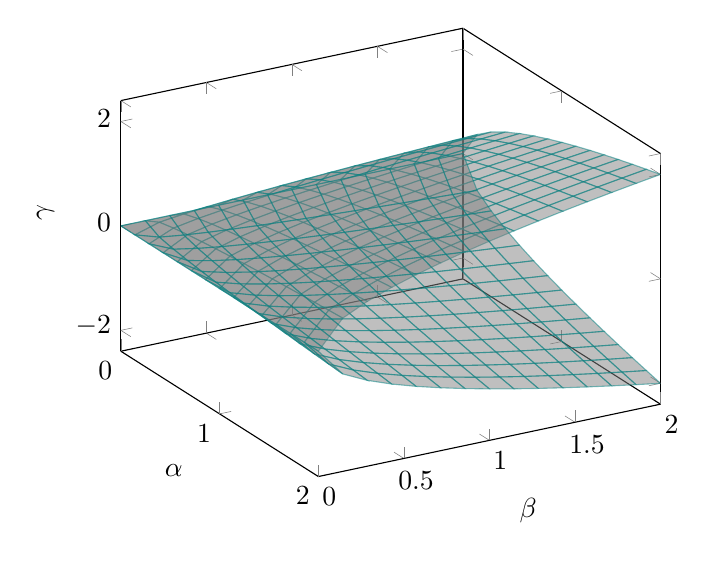
\begin{tikzpicture}
\begin{axis}[
  view={60}{30},
    xlabel=$\alpha$,
    ylabel=$\beta$,
    zlabel=$\gamma$,
]
    \addplot3 [
        surf,
        color=gray,
        faceted color = teal,
        opacity=0.5,
        samples=15,
        domain=0:2,y domain=0:2
    ] {sqrt(x*y)};
    \addplot3 [
        surf,
        color=gray,
        opacity=0.5,
        color=gray,
        faceted color = teal,
        samples=15,
        domain=0:2,y domain=0:2
    ] {-sqrt(x*y)};
\end{axis}
\end{tikzpicture}

  \end{center}
  \caption{Illustration du cône SPD pour une matrice $2\times 2$. L'ensemble des matrices de covariance vis à l'intérieur ou sur le bord du cône représenté. On peut effectuer une visualisation similaire en utilisant le code à l'adresse: \url{https://github.com/AmmarMian/simulations_hdr/blob/main/1-context/cone_spd/main.py}.}\label{fig:context-figure-spdcone}
  \end{figure}

Une caractérisation géométrique de cet espace sera développé dans la \cref{sec:context-riemann} d'où nous tirerons des outils prenant en compte la structure intrinsèque de cet espace. \\

% TODO: Regarder si d'autres propriétés sont intéressantes à ce stade

On peut également citer les propriétés suivantes, qui sont utiles pour les démonstrations de propriétés statistiques :

\begin{property}[{Lien à la moyenne}]
  \label{prop:context-definition-linkmoy}
  On a la relation suivante avec la moyenne:
  \begin{equation}
    \MCov_\Variable = \E_\Variable\left\{ \Variable\Variable^\T \right\} - \Vmoy_\Variable\Vmoy_\Variable^\T.
    \label{eq:context-definition-linkmoy}
  \end{equation}

\end{property}

\begin{property}[{Transformation linéaire}]
  \label{prop:context-definition-lineartraonsformation}
  Soit un opérateur linéaire $\mat{A}\in\R^{\Nvar\times p}$, et la variable aléatoire $\Variablebis=\mat{A}\Variable$, on a alors:
  \begin{equation}
    \MCov_\Variablebis = \mat{A}\MCov_\Variable\mat{A}^\T \in \R^{pp}.
    \label{eq:context-definition-lineartraonsformation}
  \end{equation}

\end{property}

Cette dernière propriété est notemment utile quand il s'agit de montrer comme on le verra dans le \cref{ch:robust-detection}, des invariances de tests statistiques vis-à-vis des paramètres du problème. En outre, la matrice de covariance étant une matrice SPD, on a la propriété suivante:

\begin{property}[{Diagonalisation}]
  \label{prop:context-definition-diagonalisation}
  Puisque $\MCov_\Variable$ est symmétrique réelle, alors en vertu du théorème spectral, il existe un opérateur orthogonal $\Orth\in\R^{\Nvar\Nvar}$, i.e $\Orth=\Orth^\T$ et $\Orth^{-1}=\Orth^\T$, tel que :
  \begin{equation}
    \Orth\MCov_\Variable\Orth^\T = \Diag(\eig_1\dots,\eig_\Nvar),
    \label{eq:context-definition-diagonalisation}
  \end{equation}
  où $\Diag$ est l'opérateur qui construit une matrice diagonale à partir des éléments en argument et $\{\eig_1,\dots\eig_\Nvar\}$ sont les valeurs propres de $\MCov_\Variable$.

\end{property}

\subsection{Estimation}
\label{subsec:context-covariance-estimation}

Une fois le cadre posé, un problème naturel qui émerge est l'estimation de la matrice de covariance étant donné un ensemble de données observées. Il s'agit alors à partir de mesures/observations d'estimer les tendances des variables présentes en termes de corrélations\footnote{On s'intéresse dans ce paragraphe à l'estimation sans à priori sur la loi de probabilités sous-jacente. Si l'on connait la loi à priori des données, on peut proposer le cadre de l'estimation au sens du maximum de vraisemblance comme ce sera fait en \cref{sec:context-distributions}.}.

Supposons une variable aléatoire multivariée $\Variable=[\variable_1,\dots,\variable_\Nvar]^\T$. Il est usuel d'observer ces variables sur un ensemble d'individus, ce qui nous amène à traiter un ensemble de données que l'on dénote $\Xset = \{\x_\iobs:1\leq\iobs\leq\Nobs\}$ ou bien sous forme de matrice :
\begin{equation}
  \X = \left[\x_1,\, \dots,\, \x_\Nobs \right]^\T = \left[ \begin{array}{ccc} x_{11} & \dots & x_{1\Nvar} \\ \vdots & \ddots & \vdots \\ x_{\Nvar 1} & \dots & x_{\Nvar \Nobs}   \end{array}  \right]\in\R^{\Nvar\Nobs}.
  \label{eq:context-definition-observed_data}
\end{equation}

On suppose également que ces observations sont i.i.d. Pour pouvoir calculer la covariance, il est d'abord nécessaire de s'intéresser à la moyenne:
\begin{proposition}[{Estimation de la moyenne d'un vecteur aléatoire}]
  \'Etant donné un ensemble d'observations $\X$ de la variable $\Variable$, un estimateur consistant et non-biaisé\footnote{Soit $\hat{\param}=f(\Variable)$ un estimateur d'une quantité $\param$ découlant de la variable $\Variable$. On dit que $\hat{\param}$ est \textbf{non-biaisé} si $\E_\Variable\{\hat{\param}\} = \param$. De même, on dit que l'estimateur est \textbf{consistant} si $\forall \epsilon>0,\, \displaystyle\lim_{\Nobs\to\infty} \Prob\left(|\hat{\param}-\param|>\epsilon\right)=0$.\\En d 'autres termes un estimateur non-biaisé est en moyenne autour de la vraie valeur cherchée et un estimateur consistant converge vers la vraie valeur avec suffisamment d'observations.} de la moyenne est:
  \begin{equation}
    \hat{\Vmoy}_\Variable = \frac{1}{\Nobs}\sum_{\iobs=1}^{\Nobs} \x_\iobs.
    \label{eq:context-estimation-moyenne}
  \end{equation}
\end{proposition}

\begin{remark}
  Il est facile de montrer, en vertu de la loi des grands nombres que pour $\Nobs\to\infty$:
  $$
  \hat{\Vmoy}_\Variable \approx \E_\Variable\{\Variable\}=\Vmoy_\Variable.
  $$
\end{remark}


\begin{remark}
  On peut retrouver le côté non-biaisé en prenant l'espérance de l'estimateur\footnote{On se permettra à partir de maintenant d'utiliser par simplification l'opérateur espérance sur les valeurs observées des variables sans aller chercher la variable aléatoire sous-jacente. On comprends que l'on regarde l'espérance d'une fonction des variables aléatoires et non de valeurs précises observées.}:
  $$
  \E_\Variable\left\{\hat{\Vmoy}_\Variable\right\} = \E_\Variable\left\{\frac{1}{\Nobs}\sum_{\iobs=1}^{\Nobs}\x_\iobs\right\} = \Vmoy_\Variable.
  $$
\end{remark}


Afin d'estimer la matrice de covariance, on peut en partant de cette première estimation avoir l'estimateur suivant:

\begin{proposition}[{Estimateur de la matrice de covariance}]
  \'Etant donné un ensemble d'observations $\X$ de la variable $\Variable$, un estimateur consistant et non-biaisé de la matrice de covariance est la scm:
  \begin{equation}
    \hat{\MCov}_\Variable =  \frac{1}{\Nobs-1}\sum_{\iobs=1}^{\Nobs} \left(\x_\iobs-\hat{\Vmoy}_x\right)\left(\x_\iobs-\hat{\Vmoy}_x\right)^\T.
    \label{eq:context-estimation-covariance}
  \end{equation}
\end{proposition}


\begin{remark}[{Caractère non-biaisé}]
  On remarque que le coefficient $(N-1)$ et non $N$ dans la fraction. Cela permet à notre estimateur d'être non biaisé. en effet, on peut montrer que:
$$
  E_\Variable\left\{\left(\x_\iobs-\hat{\Vmoy}_\Variable\right)\left(\x_\iobs-\hat{\Vmoy}_\Variable\right)^\T\right\} = \frac{N-1}{N}\MCov_\Variable.
$$
Il est ainsi nécessaire de compenser par le facteur $\frac{N}{N-1}$ pour obtenir un estimateur non-biaisé:


%  \vspace{-2em}
%   \begin{proof}
%   En effet, calculons l'espérance de celui-ci:
%   \begin{align*}
%     \E_\Variable\left\{ \hat{\MCov}_\Variable \right \} & =  \frac{1}{\Nobs-1}\sum_{\iobs=1}^{\Nobs} \E_\Variable\left\{\left(\x_\iobs-\hat{\Vmoy}_x\right)\left(\x_\iobs-\hat{\Vmoy}_x\right)^\T\right\}.
%   \end{align*}
%
% Développons l'expression à l'intérieur de l'espérance :
%   \begin{align*}
%     \left(\x_\iobs-\hat{\Vmoy}_\Variable\right)\left(\x_\iobs-\hat{\Vmoy}_\Variable\right)^\T &= \x_\iobs\x_\iobs^\T - \x_\iobs\hat{\Vmoy}_\Variable^\T - \hat{\Vmoy}_\Variable\x_\iobs^\T + \hat{\Vmoy}_\Variable\hat{\Vmoy}_\Variable^\T.
%   \end{align*}
%
%   En prenant l'espérance terme par terme et en utilisant le fait que les observations sont i.i.d :
%
%     \textbf{Terme 1 :} $\E_\Variable\left\{\x_\iobs\x_\iobs^\T\right\} = \MCov_\Variable + \Vmoy_\Variable\Vmoy_\Variable^\T$ en vertu de la \cref{prop:context-definition-linkmoy}.
%
%   \textbf{Terme 2 :} Sachant que $\hat{\Vmoy}_\Variable = \frac{1}{\Nobs}\sum_{j=1}^{\Nobs} \x_j$ :
%   \begin{align*}
%     \E_\Variable\left\{\x_\iobs\hat{\Vmoy}_\Variable^\T\right\} &= \E_\Variable\left\{\x_\iobs \cdot \frac{1}{\Nobs}\sum_{j=1}^{\Nobs} \x_j^\T\right\} = \frac{1}{\Nobs}\sum_{j=1}^{\Nobs} \E_\Variable\left\{\x_\iobs\x_j^\T\right\}
%   \end{align*}
%
%   Comme les observations sont i.i.d :
%   \begin{itemize}
%     \item Si $\iobs = j$ : $\E_\Variable\left\{\x_\iobs\x_j^\T\right\} = \MCov_\Variable + \Vmoy_\Variable\Vmoy_\Variable^\T$
%     \item Si $\iobs \neq j$ : $\E_\Variable\left\{\x_\iobs\x_j^\T\right\} = \Vmoy_\Variable\Vmoy_\Variable^\T$
%   \end{itemize}
%
%   \begin{align*}
%     \text{Donc :} \E_\Variable\left\{\x_\iobs\hat{\Vmoy}_\Variable^\T\right\} &= \frac{1}{\Nobs}\left[(\MCov_\Variable + \Vmoy_\Variable\Vmoy_\Variable^\T) + (\Nobs-1)\Vmoy_\Variable\Vmoy_\Variable^\T\right] = \frac{1}{\Nobs}\MCov_\Variable + \Vmoy_\Variable\Vmoy_\Variable^\T
%   \end{align*}
%
%   \textbf{Terme 3 :} Par symétrie : $\E_\Variable\left\{\hat{\Vmoy}_\Variable\x_\iobs^\T\right\} = \frac{1}{\Nobs}\MCov_\Variable + \Vmoy_\Variable\Vmoy_\Variable^\T$
%
%
%   \begin{align*}
%     \text{\bfseries Terme 4 :} \E_\Variable\left\{\hat{\Vmoy}_\Variable\hat{\Vmoy}_\Variable^\T\right\} &= \E_\Variable\left\{\frac{1}{\Nobs^2}\sum_{j=1}^{\Nobs}\sum_{\iobs=1}^{\Nobs} \x_j\x_\iobs^\T\right\} = \frac{1}{\Nobs^2}\sum_{j=1}^{\Nobs}\sum_{\iobs=1}^{\Nobs} \E_\Variable\left\{\x_j\x_\iobs^\T\right\}
%   \end{align*}
%
%   Il y a $\Nobs$ termes avec $j = \iobs$ et $\Nobs^2 - \Nobs$ termes avec $j \neq \iobs$, d'où :
%   \begin{align*}
%     \E_\Variable\left\{\hat{\Vmoy}_\Variable\hat{\Vmoy}_\Variable^\T\right\} &= \frac{1}{\Nobs^2}\left[\Nobs(\MCov_\Variable + \Vmoy_\Variable\Vmoy_\Variable^\T) + (\Nobs^2-\Nobs)\Vmoy_\Variable\Vmoy_\Variable^\T\right] = \frac{1}{\Nobs}\MCov_\Variable + \Vmoy_\Variable\Vmoy_\Variable^\T
%   \end{align*}
%
%   \begin{align*}
%     \text{Donc} &\E_\Variable\left\{\left(\x_\iobs-\hat{\Vmoy}_\Variable\right)\left(\x_\iobs-\hat{\Vmoy}_\Variable\right)^\T\right\} \\
%     &= (\MCov_\Variable + \Vmoy_\Variable\Vmoy_\Variable^\T) - 2\left(\frac{1}{\Nobs}\MCov_\Variable + \Vmoy_\Variable\Vmoy_\Variable^\T\right) + \left(\frac{1}{\Nobs}\MCov_\Variable + \Vmoy_\Variable\Vmoy_\Variable^\T\right) \\
%     &= \MCov_\Variable - \frac{1}{\Nobs}\MCov_\Variable = \frac{\Nobs-1}{\Nobs}\MCov_\Variable\\
%     \text{Conclusion :} & \E_\Variable\left\{ \hat{\MCov}_\Variable \right \} = \frac{1}{\Nobs-1}\sum_{\iobs=1}^{\Nobs} \frac{\Nobs-1}{\Nobs}\MCov_\Variable \\
%     &= \frac{1}{\Nobs-1} \cdot \Nobs \cdot \frac{\Nobs-1}{\Nobs}\MCov_\Variable = \MCov_\Variable.
%   \end{align*}
%
%   L'estimateur est donc bien non-biaisé, ce qui justifie l'utilisation du coefficient $\frac{1}{\Nobs-1}$ plutôt que $\frac{1}{\Nobs}$.
% \end{proof}
\end{remark}


\begin{remark}
Une fois que l'on connait $E_\Variable\left\{\left(\x_\iobs-\hat{\Vmoy}_\Variable\right)\left(\x_\iobs-\hat{\Vmoy}_\Variable\right)^\T\right\}$, on peut utiliser la loi des grands nombres pour dire que lorsque $\Nobs\to\infty$\footnote{il ne s'agit pas d'une démonstration de la consistance théorique, qui requiert des conditions de régularité sur la d.d.p sous-jacente mais cela illustre un comportement en ce sens.}:
  \begin{align*}
    \hat{\MCov}_\Variable &= \frac{\Nobs}{\Nobs-1}\times\frac{1}{\Nobs} \sum_{\iobs=1}^\Nobs\left(\x_\iobs-\hat{\Vmoy}_\Variable\right)\left(\x_\iobs-\hat{\Vmoy}_\Variable\right)^\T \\
    & \approx  \frac{\Nobs}{\Nobs-1} E_\Variable\left\{\left(\x_\iobs-\hat{\Vmoy}_\Variable\right)\left(\x_\iobs-\hat{\Vmoy}_\Variable\right)^\T\right\}  = \MCov_\Variable.
\end{align*}
\end{remark}


Il est intéressant de regarder à travers une simulation numérique, la convergence de nos deux estimateurs dans le régime $\Nobs\to\infty$. Pour ce faire, nous simulons des données de moyenne $\Vmoy_\Variable = [1,\dots,1]^\T$ et de matrice de covariance $\MCov_\Variable=\Id{\Nvar}$ en générant des données gaussiennes de moyenne $1$ et variance $1$ pour chaque observation $x_{\ivar\iobs}$. On représente alors en \cref{fig:context-estimation-errorscm}, l'erreur d'estimation\footnote{On utilise pour cela la norme euclidienne d'ordre 2 mais nous verrons dans la \cref{sec:context-riemann} que ce choix peut être discuté.} en fonction du nombre d'observations $\Nobs$. Même si ces simulations ne suffisent pas à elles seules à montrer la consistance et la convergence de nos estimateurs aux vraies paramètres de nos variables aléatoires, on peut observer à la fois une baisse de l'erreur en moyenne mais également que la variance de l'erreur diminue. On caractérisera ces deux comportements en \cref{sec:context-distributions} dans un cadre où l'on ajoute un à priori sur la distribution sous-jacente des données.
% TODO: ne pas oublier de faire consistance avec à-priori gaussien et elliptique si possible.

\begin{figure*}[h]
    \begin{center}
    % This file was created with matplot2tikz v0.5.3.
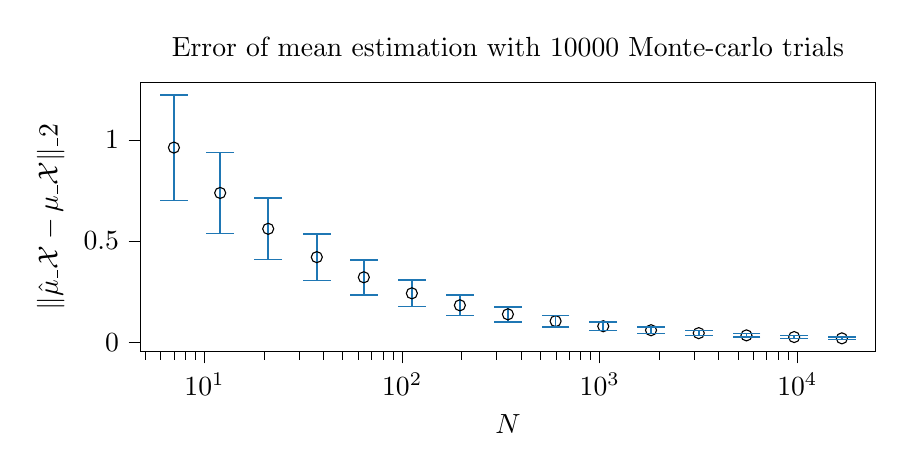
\begin{tikzpicture}

\definecolor{darkgray176}{RGB}{176,176,176}
\definecolor{steelblue31119180}{RGB}{31,119,180}

\begin{axis}[
width=0.9\textwidth,
height=5cm,
log basis x={10},
tick align=outside,
tick pos=left,
title={Error of mean estimation with 10000 Monte-carlo trials},
x grid style={darkgray176},
xlabel={\(\displaystyle N\)},
xmin=4.74327639380337, xmax=24803.3195269196,
xmode=log,
xtick style={color=black},
y grid style={darkgray176},
ylabel={\(\displaystyle \|\hat{\boldsymbol{\mu}}\_\mathcal{X} - \boldsymbol{\mu}\_\mathcal{X}\|\_2\)},
ymin=-0.0461003164651899, ymax=1.28319327993008,
ytick style={color=black}
]
\addplot [draw=black, mark=o, only marks]
table{%
x  y
7 0.961809938446161
12 0.737728543463078
21 0.560616951169621
37 0.420661897373797
64 0.32120978405099
112 0.242018240638433
196 0.182805838986852
343 0.138405338128785
598 0.104765688177838
1042 0.0794917535174116
1818 0.0598006596884444
3170 0.0453866342512824
5528 0.0343647504602777
9639 0.026099922904704
16807 0.0196559171311048
};
\path [draw=steelblue31119180, semithick]
(axis cs:7,0.700849033162032)
--(axis cs:7,1.22277084373029);

\path [draw=steelblue31119180, semithick]
(axis cs:12,0.537975705847932)
--(axis cs:12,0.937481381078224);

\path [draw=steelblue31119180, semithick]
(axis cs:21,0.409881143046451)
--(axis cs:21,0.711352759292791);

\path [draw=steelblue31119180, semithick]
(axis cs:37,0.306090426059901)
--(axis cs:37,0.535233368687693);

\path [draw=steelblue31119180, semithick]
(axis cs:64,0.234693244705277)
--(axis cs:64,0.407726323396703);

\path [draw=steelblue31119180, semithick]
(axis cs:112,0.176615269618465)
--(axis cs:112,0.307421211658401);

\path [draw=steelblue31119180, semithick]
(axis cs:196,0.133295627068537)
--(axis cs:196,0.232316050905168);

\path [draw=steelblue31119180, semithick]
(axis cs:343,0.101071846947206)
--(axis cs:343,0.175738829310364);

\path [draw=steelblue31119180, semithick]
(axis cs:598,0.0764314707238397)
--(axis cs:598,0.133099905631837);

\path [draw=steelblue31119180, semithick]
(axis cs:1042,0.0578812731877006)
--(axis cs:1042,0.101102233847123);

\path [draw=steelblue31119180, semithick]
(axis cs:1818,0.0435629040530663)
--(axis cs:1818,0.0760384153238226);

\path [draw=steelblue31119180, semithick]
(axis cs:3170,0.0331333015828912)
--(axis cs:3170,0.0576399669196737);

\path [draw=steelblue31119180, semithick]
(axis cs:5528,0.0251640440466649)
--(axis cs:5528,0.0435654568738906);

\path [draw=steelblue31119180, semithick]
(axis cs:9639,0.0190071644585281)
--(axis cs:9639,0.0331926813508799);

\path [draw=steelblue31119180, semithick]
(axis cs:16807,0.0143221197345949)
--(axis cs:16807,0.0249897145276147);

\addplot [semithick, steelblue31119180, mark=-, mark size=5, mark options={solid}, only marks]
table {%
7 0.700849033162032
12 0.537975705847932
21 0.409881143046451
37 0.306090426059901
64 0.234693244705277
112 0.176615269618465
196 0.133295627068537
343 0.101071846947206
598 0.0764314707238397
1042 0.0578812731877006
1818 0.0435629040530663
3170 0.0331333015828912
5528 0.0251640440466649
9639 0.0190071644585281
16807 0.0143221197345949
};
\addplot [semithick, steelblue31119180, mark=-, mark size=5, mark options={solid}, only marks]
table {%
7 1.22277084373029
12 0.937481381078224
21 0.711352759292791
37 0.535233368687693
64 0.407726323396703
112 0.307421211658401
196 0.232316050905168
343 0.175738829310364
598 0.133099905631837
1042 0.101102233847123
1818 0.0760384153238226
3170 0.0576399669196737
5528 0.0435654568738906
9639 0.0331926813508799
16807 0.0249897145276147
};
\end{axis}

\end{tikzpicture}

    % This file was created with matplot2tikz v0.5.3.
\begin{tikzpicture}

\definecolor{darkgray176}{RGB}{176,176,176}
\definecolor{steelblue31119180}{RGB}{31,119,180}

\begin{axis}[
width=0.9\textwidth,
height=5cm,
log basis x={10},
tick align=outside,
tick pos=left,
x grid style={darkgray176},
xlabel={\(\displaystyle N\)},
xmin=4.74327639380337, xmax=24803.3195269196,
xmode=log,
xtick style={color=black},
y grid style={darkgray176},
ylabel={\(\displaystyle \|\hat{\MCov}_\Variable - \MCov_\Variable \|_2\)},
ymin=-0.13262423207483, ymax=3.87655604361312,
ytick style={color=black}
]
\addplot [draw=black, mark=o, only marks]
table{%
x  y
7 2.96644841886547
12 2.21671185618484
21 1.64709208228737
37 1.23397594189885
64 0.935112170973186
112 0.703404726719878
196 0.531310446912574
343 0.400325303184381
598 0.303923396605062
1042 0.230114283599226
1818 0.174038501677559
3170 0.131597391353147
5528 0.0998109498844136
9639 0.0753512175742832
16807 0.0572766951577409
};
\path [draw=steelblue31119180, semithick]
(axis cs:7,2.23857626119455)
--(axis cs:7,3.69432057653639);

\path [draw=steelblue31119180, semithick]
(axis cs:12,1.76497915252549)
--(axis cs:12,2.6684445598442);

\path [draw=steelblue31119180, semithick]
(axis cs:21,1.35747786948254)
--(axis cs:21,1.9367062950922);

\path [draw=steelblue31119180, semithick]
(axis cs:37,1.0374123409997)
--(axis cs:37,1.43053954279801);

\path [draw=steelblue31119180, semithick]
(axis cs:64,0.795915368703914)
--(axis cs:64,1.07430897324246);

\path [draw=steelblue31119180, semithick]
(axis cs:112,0.603021809771917)
--(axis cs:112,0.803787643667839);

\path [draw=steelblue31119180, semithick]
(axis cs:196,0.458345285906057)
--(axis cs:196,0.604275607919091);

\path [draw=steelblue31119180, semithick]
(axis cs:343,0.345034478896582)
--(axis cs:343,0.455616127472181);

\path [draw=steelblue31119180, semithick]
(axis cs:598,0.262460291581848)
--(axis cs:598,0.345386501628276);

\path [draw=steelblue31119180, semithick]
(axis cs:1042,0.198925436760575)
--(axis cs:1042,0.261303130437877);

\path [draw=steelblue31119180, semithick]
(axis cs:1818,0.150584064767169)
--(axis cs:1818,0.197492938587949);

\path [draw=steelblue31119180, semithick]
(axis cs:3170,0.114065796158437)
--(axis cs:3170,0.149128986547856);

\path [draw=steelblue31119180, semithick]
(axis cs:5528,0.0865643002479931)
--(axis cs:5528,0.113057599520834);

\path [draw=steelblue31119180, semithick]
(axis cs:9639,0.0652154542494471)
--(axis cs:9639,0.0854869808991193);

\path [draw=steelblue31119180, semithick]
(axis cs:16807,0.0496112350018946)
--(axis cs:16807,0.0649421553135873);

\addplot [semithick, steelblue31119180, mark=-, mark size=5, mark options={solid}, only marks]
table {%
7 2.23857626119455
12 1.76497915252549
21 1.35747786948254
37 1.0374123409997
64 0.795915368703914
112 0.603021809771917
196 0.458345285906057
343 0.345034478896582
598 0.262460291581848
1042 0.198925436760575
1818 0.150584064767169
3170 0.114065796158437
5528 0.0865643002479931
9639 0.0652154542494471
16807 0.0496112350018946
};
\addplot [semithick, steelblue31119180, mark=-, mark size=5, mark options={solid}, only marks]
table {%
7 3.69432057653639
12 2.6684445598442
21 1.9367062950922
37 1.43053954279801
64 1.07430897324246
112 0.803787643667839
196 0.604275607919091
343 0.455616127472181
598 0.345386501628276
1042 0.261303130437877
1818 0.197492938587949
3170 0.149128986547856
5528 0.113057599520834
9639 0.0854869808991193
16807 0.0649421553135873
};
\end{axis}

\end{tikzpicture}

  \end{center}
  \provScmmeanQR[.5cm]
    \caption{\'Evolution de l'erreur d'estimation de la moyenne et de la matrice de covariance en fonction de $\Nobs$ pour $\Nvar=7$. Les marqueurs correspondent à la moyenne de l'erreur d'estimation et les barres correspondent à la déviation standard de cette même erreur. Le nombre de tirages de monte-carlo est de $ 10^4$. \provScmcov}
  \label{fig:context-estimation-errorscm}
\end{figure*}



\subsection{Estimation régularisée}
\label{subsec:context-covariance-regularized-estimation}

  


L'estimateur classique de la matrice de covariance donné par \cref{eq:context-definition-covariance-formula} présente des limitations importantes dans certains régimes dimensionnels. En effet, lorsque le nombre de variables $\Nvar$ devient comparable ou supérieur au nombre d'observations $\Nobs$, cet estimateur souffre de plusieurs défauts majeurs qui compromettent sa fiabilité pratique.

Le premier problème concerne le rang de la matrice estimée. Dans le cas extrême où $\Nvar > \Nobs$, la matrice $\hat{\MCov}_\Variable$ est nécessairement singulière, car elle est construite comme une somme de $\Nobs$ matrices de rang 1. Plus précisément, son rang est au plus $\min(\Nvar, \Nobs-1)$\footnote{Le facteur $N-1$ plutôt que $N$ est dû au fait que l'on additionne des matrices construites à partir d'observations dont on a soustrait la moyenne et donc introduit une relation linéaire d'ordre 1.}, ce qui la rend non-inversible lorsque $\Nvar \geq \Nobs$. Cette singularité pose des difficultés majeures pour de nombreuses applications statistiques nécessitant l'inversion de la matrice de covariance, comme l'analyse discriminante ou certaines méthodes de classification. Au-delà de ce problème de rang, même dans le régime sous-déterminé où $\Nvar < \Nobs$ mais où le rapport $\Nvar/\Nobs$ n'est pas négligeable\footnote{Ce qui sera le cas dans de nombreuses approches basé sur une estimation de la covariance en apprentissage profond. Voir pour cela le \cref{ch:spdnet}.}, l'estimateur empirique souffre d'une grande variabilité. Cette variabilité se manifeste notamment par une dispersion importante des valeurs propres de $\hat{\MCov}_\Variable$ autour de celles de la vraie matrice $\MCov_\Variable$. Cela peut être analysé au travers de la notion de conditionnement:

\begin{figure}
  \begin{center}
      \begin{minipage}{0.45\textwidth}
        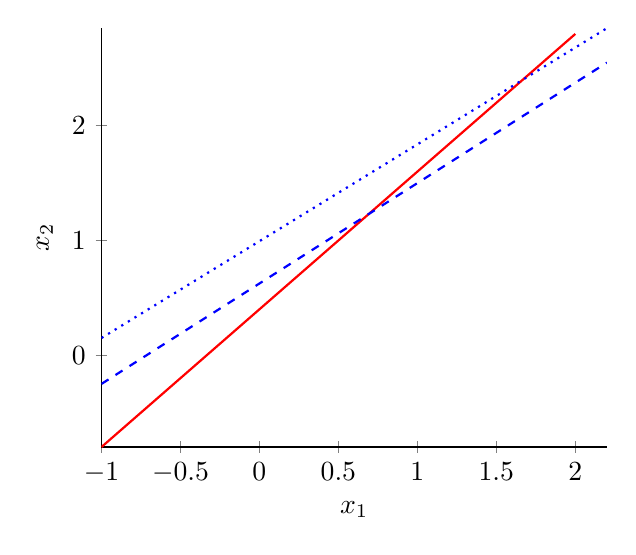
\begin{tikzpicture}
\begin{axis}[
    width=8cm,
    xlabel={$x_1$},
    ylabel={$x_2$},
    axis lines=left,
    axis line style={-},
]
\addplot[red, thick] coordinates {(-1, -0.8) (2, 2.8)};
\addplot[blue, thick, dashed] coordinates {(-1, -0.25) (2.2, 2.55)};
\addplot[blue, thick, dotted] coordinates {(-1, 0.15) (2.2, 2.85)};
\end{axis}
\end{tikzpicture}

      \end{minipage}
      \begin{minipage}{0.45\textwidth}
        
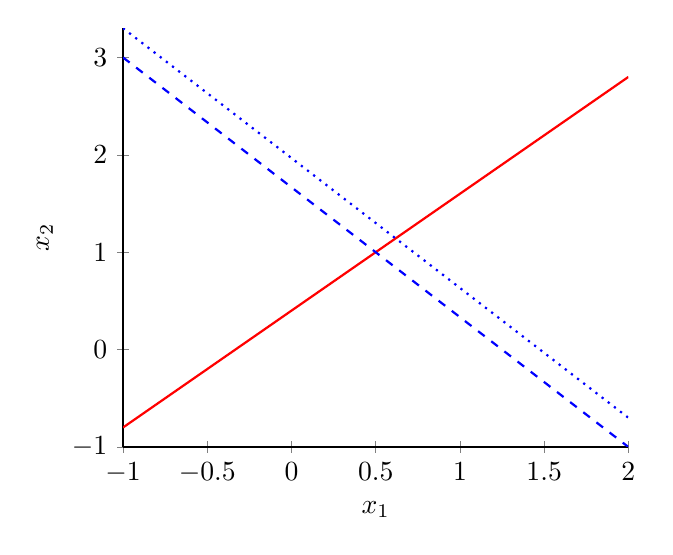
\begin{tikzpicture}
\begin{axis}[
    width=8cm,
    xlabel={$x_1$},
    ylabel={$x_2$},
    axis lines=left,
    axis line style={-},
]
\addplot[red, thick] coordinates {(-1, -0.8) (2, 2.8)};
  \addplot[blue, thick, dashed] coordinates {(-1, 3) (2, -1)};
  \addplot[blue, thick, dotted] coordinates {(-1, 3.3) (2, -0.7)};
\end{axis}
\end{tikzpicture}

      \end{minipage}
      \vspace{-2em}
      \end{center}
  \caption{Illustration visuelle du conditionnement d'un système linéaire dans le cas où $\mat{A}\in\R^{2\times 2}$. La solution correspond à l'intersection des droites continues (-) et en pointillés (- -). Une perturbation sur $\vector{b}$ déplace la droite (- -) en (..). À gauche: le cas d'une matrice mal conditionnée car la solution bouge beaucoup à cause de la perturbation. À droite: la perturbation a moins d'effet sur la solution.}\label{fig:context-estimation-condition}
\end{figure}

  \begin{definition}[{Conditionnement d'une matrice à l'inversion}]
    Le conditionnement d'une matrice $\mat{A}\in\R^{pq}$  est donné par :
    \begin{equation}
      \Cond(\mat{A}) = \|\mat{A}\|_2\|\mat{A}^{-1}\|_2.
      \label{eq:context-estimation-condition}
    \end{equation}
    
  \end{definition}

  \begin{remark}
Il correspond à un nombre quantifiant la sensibilité de la solution au système linéaire:
$$
    \mat{A}\x = \vector{b},
$$
    où $\x\in\R^q$ est la solution cherchée et $\vector{b}\in\R^q$ est un vecteur de constantes. En effet, supposant une erreur d'approximation $\vector{e}\in\R^q$ sur le vecteur $\vector{b}$, résoudre en pratique le système :
  $$
      \mat{A}\x = \vector{b}+\vector{e},
  $$
    provoque une erreur sur la solution de l'ordre $\mat{A}^{-1}\vector{e}$. En quantifiant le ratio entre l'erreur relative sur la solution et sur $\vector{b}$ :
    $$
     \epsilon(\vector{e}) =  \left. \frac{\|\mat{A}^{-1}\vector{e}\|_2}{\| \mat{A}^{-1}\vector{b}\|_2} \displaystyle \middle/ \frac{\|\vector{e}\|_2}{\| \vector{b}\|_2} \right. ,
    $$

    on a pour $\vector{e}\neq \vector{0}$ et $\vector{b}\neq\vector{0}$, $\max_{\vector{e}}\epsilon(\vector{e})=\Cond(\mat{A})$.

    Ainsi, ce nombre nous donne une information sur la praticabilité d'une matrice obtenue par estimation vis à vis de problèmes nécessitant son inversion. Ce principe est illustré en \cref{fig:context-estimation-condition}.
  \end{remark}

Notamment dans le cas de matrices carrée symétriques, on a le résultat suivant :

\begin{proposition}[{Conditionnement d'une matrice symmétrique}]
  Soit une matrice $\mat{A}\in\R^{\Nvar\Nvar}$ tel que $\mat{A}=\mat{A}^\T$, on peut calculer le conditionnement de cette matrice vis-à-vis de l'inversion donnée en \cref{eq:context-estimation-condition} avec:
    \begin{equation}
      \Cond(\mat{A}) = \frac{\max |\eigset(\mat{A})|}{\min |\eigset(\mat{A})|},
      \label{eq:context-estimation-conditionspd}
    \end{equation}
  où $\eigset(\mat{A})$ est l'ensemble des valeurs propres de $\mat{A}$.
\end{proposition}




Si l'on revient à l'estimation de notre matrice de covariance, on peut quantifier la dispersion en pratique : en simulant des données aléatoires de la même façon que précédemment en \cref{subsec:context-covariance-estimation} avec une moyenne et matrice covariance connues. Plutôt que de regarder l'erreur d'estimation, on s'intéresse au conditionnement de la matrice estimée en \cref{fig:context-estimation-cond}. On s'aperçoit alors que dés que la taille de la matrice approche ou dépasse le nombre d'observations, le conditionnement de la matrice explose, i.e, les valeurs propres ont une très grande dispersion, ce qui est problématique pour un certain nombre d'applications dépendant d'une SVD de cette matrice, tel que l'analyse en composantes principales par exemple. \\

\begin{figure}[h]
  \begin{center}
        % This file was created with matplot2tikz v0.5.3.
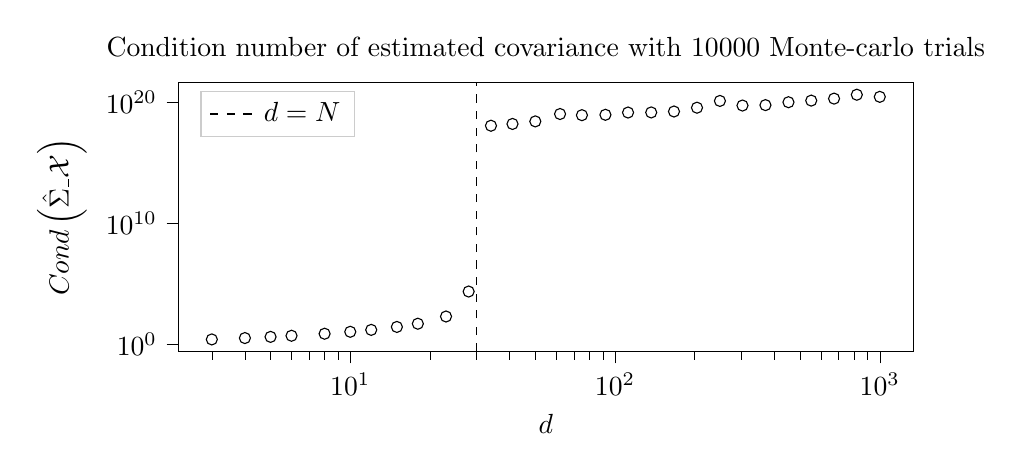
\begin{tikzpicture}

\definecolor{darkgray176}{RGB}{176,176,176}
\definecolor{lightgray204}{RGB}{204,204,204}

\begin{axis}[
width=0.9\textwidth,
height=5cm,
legend cell align={left},
legend style={
  fill opacity=0.8,
  draw opacity=1,
  text opacity=1,
  at={(0.03,0.97)},
  anchor=north west,
  draw=lightgray204
},
log basis x={10},
log basis y={10},
tick align=outside,
tick pos=left,
title={Condition number of estimated covariance with 10000 Monte-carlo trials},
x grid style={darkgray176},
xlabel={\(\displaystyle d\)},
xmin=2.2437647322819, xmax=1337.03857487278,
xmode=log,
xtick style={color=black},
y grid style={darkgray176},
ylabel={\(\displaystyle \operatorname{Cond}\left(\hat{\boldsymbol{\Sigma}}\_\mathcal{X}\right)\)},
ymin=0.22380594276999, ymax=4.1309909352877e+21,
ymode=log,
ytick style={color=black}
]
\addplot [draw=black, forget plot, mark=o, only marks]
table{%
x  y
3 2.30128721449648
4 2.98980176023402
5 3.74725148388153
6 4.6273062005471
8 6.80978228176998
10 9.85053405764688
12 14.1914261593259
15 24.8541084638651
18 45.8675117285121
23 181.624000745188
28 21118.5385109043
34 1.09423163871398e+18
41 1.54003337498655e+18
50 2.50285206785319e+18
62 1.02082277017018e+19
75 8.1696391406987e+18
92 8.78584488032868e+18
112 1.35351469825842e+19
137 1.37578020462997e+19
167 1.64652490481264e+19
204 3.4004576745693e+19
249 1.23230576162333e+20
303 5.12553978317069e+19
370 5.56209683272156e+19
452 9.65397291811529e+19
551 1.31245394055025e+20
672 1.91723632520982e+20
819 4.01749210190887e+20
1000 2.688261444791e+20
};
\addplot [semithick, black, dashed]
table {%
30 0.22380594276999
30 4.1309909352877e+21
};
\addlegendentry{$d=N$}
\end{axis}

\end{tikzpicture}

      \end{center}
  \provScmcondQR[.5cm]
  \caption{\'Evolution du conditionnement de la matrice estimée  par SCM pour une taille croissante de variables $\Nvar$ avec $\Nobs=30$. Les marqueurs indique la moyenne du conditionnement sur 50 tirages de monte-carlo. \provScmcond}
  \label{fig:context-estimation-cond}
\end{figure}



Pour pallier les défauts de l'estimateur empirique en haute dimension, \sidecite[0cm]{LedoitWolf2004} proposent un estimateur régularisé de la forme :

\begin{definition}[{Estimateur de Ledoit-Wolf}]
\begin{equation}
  \hat{\MCov}_\Variable^{\text{LW}}(\coefledoitwolf) = (1-\coefledoitwolf) \hat{\MCov}_\Variable + \coefledoitwolf \targetledoitwolf
\label{eq:context-ledoit-wolf}
\end{equation}
où $\coefledoitwolf \in [0,1]$ est un coefficient de régularisation et $\targetledoitwolf$ est une matrice cible (\textit{target}) de même dimension que $\hat{\MCov}_\Variable$.
\end{definition}

L'idée fondamentale de cette approche consiste à contracter l'estimateur empirique vers une matrice cible $\targetledoitwolf$ possédant de meilleures propriétés de conditionnement. Le choix le plus courant pour cette matrice cible est la matrice identité mise à l'échelle : $\targetledoitwolf = \frac{\Tr(\hat{\MCov}_\Variable)}{\Nvar} \mathbf{I}_\Nvar$. Cette cible correspond à l'hypothèse que toutes les variables ont la même variance (égale à la variance moyenne) et sont non corrélées entre elles. Ainsi, l'estimateur se veut être un compromis entre l'estimation SCM et une hypothèse de variables faiblement corrélées.

Le choix du coefficient $\coefledoitwolf$ est fait à priori mais si l'on définit un critère de eqm sur la qualité de l'estimation:
\begin{equation}
  \loss(\hat{\MCov}_\Variable(\coefledoitwolf), \MCov_\Variable) = \| \hat{\MCov}_\Variable(\coefledoitwolf) - \MCov_\Variable \|_\frob^2
  \label{eq:context-estimation-losslwf}
\end{equation}
sous le modèle donné en \cref{eq:context-ledoit-wolf}, on peut alors vouloir trouver l'optimal au sens statistique.
%TODO: Verify this loss, notably squared

Pour ce faire, nous nous intéressons à l'espérance du critère défini en \cref{eq:context-estimation-losslwf}:
$$
  \risk(\coefledoitwolf) = \E_\Variable\left\{\loss(\hat{\MCov}_\Variable(\coefledoitwolf), \MCov_\Variable)\right\},
$$

et l'on veut résoudre:
\begin{equation}
  \coefledoitwolf^\star = \arg\min_\coefledoitwolf \risk(\coefledoitwolf).
\end{equation}

%TODO : parler de l'estimation de alpha optimal dans la partie ddp

% On peut alors montrer en développant les termes de la norme et solvant $\frac{\partial\risk(\coefledoitwolf) }{\partial\coefledoitwolf}=0$ que la solution optimale est atteinte en:
%
% $$\coefledoitwolf^\opt = \frac{\E\left\{\|\hat{\MCov}_\Variable - \MCov_\Variable\|_\frob^2\right\} - \E\left\{\Tr\left((\hat{\MCov}_\Variable - \MCov_\Variable)(\targetledoitwolf - \MCov_\Variable)^T\right)\right\}}{\|\targetledoitwolf - \MCov_\Variable\|_\frob^2}$$
% %TODO: verify this
%
% En exprimant cette solution en termes des éléments matriciels individuels et en utilisant les propriétés d'espérance des estimateurs empiriques, cette expression se reformule sous la forme pratique suivante:
%
%
% \begin{proposition}[{Estimation optimale du coefficient de régularisation}]
% Le coefficient optimal $\coefledoitwolf^*$ au sens de la minimisation de l'erreur quadratique moyenne est donné par :
% \begin{equation}
% \coefledoitwolf^* = \frac{\sum_{i,j} \text{Var}(\hat{\sigma}_{ij})}{\sum_{i,j} (\hat{\sigma}_{ij} - t_{ij})^2}
% \label{eq:context-alpha-optimal}
% \end{equation}
% où $\hat{\sigma}_{ij}$ et $t_{ij}$ désignent respectivement les éléments $(i,j)$ des matrices $\hat{\MCov}_\Variable$ et $\targetledoitwolf$.
% \end{proposition}
%



\begin{figure}
  \begin{tikzpicture}
\begin{axis}[
    width=8cm,
    height=4cm,
    xlabel={$\coefledoitwolf$},
    ylabel={$\risk(\coefledoitwolf)$},
    xmin=0, xmax=1,
    ymin=0, ymax=3,
    grid=none,
    grid style={gray!30},
    legend style={
        fill=none,
        draw=none,
        at={(0,1.1)},
        anchor=south west,
    },
    legend cell align={left},
    % Custom axis labels
    xtick={0,1},
    ymajorticks=false,
    axis lines=left,
    axis line style={-},
]


% Variance curve - matches the dashed line in your figure
% Decreases from 1.8 to 1.2 with gentle quadratic curvature
\addplot[
    thick,
    dashed,
    domain=0.001:1,
    samples=100
] {.2-ln(.25+x)};
\addlegendentry{Variance}

% Squared Bias curve - matches the dotted line in your figure  
% Increases from 0.3 to 1.3 with accelerating quadratic growth
\addplot[
    thick,
    dotted,
    domain=0:1,
    samples=100
] {0.01 - 0.2*x + 2.4*x^2};
\addlegendentry{Bias$^2$}

% Mean Squared Error - matches the solid U-shaped curve in your figure
% Sum of variance and bias: (1.8-0.9x+0.3x²) + (0.3-0.7x+1.7x²) = 2.1-1.6x+2.0x²
% Minimum at x=0.4 with value 1.78
\addplot[
    thick,
    solid,
    domain=0:1,
    samples=100
] {3*(x-0.4)^2+1.1};
\addlegendentry{EQM}

% Key estimation points with geometric markers

% Sample covariance matrix (left endpoint, λ=0)
% Square symbol represents the unregularized estimator
\addplot[
    only marks,
    mark=square*,
    mark size=2pt,
    mark options={fill=black}
] coordinates {(0, 1.6)};

% Identity target matrix (right endpoint, λ=1) 
% Diamond symbol represents the fully shrunk estimator
\addplot[
    only marks,
    mark=diamond*,
    mark size=2pt,
    mark options={fill=black}
] coordinates {(1, 2.2)};

% Optimal Ledoit-Wolf estimator (minimum of MSE curve at λ=0.4)
% Circle symbol represents the optimal compromise
\addplot[
    only marks,
    mark=*,
    mark size=2pt,
    mark options={fill=black}
] coordinates {(0.4, 1.1)};

% Annotations for the key estimation points
% Using axis coordinates ensures precise positioning relative to data points
\node[above, anchor=south west] at (axis cs:0, 1.65) {\tiny$\hat{\MCov}_\Variable$};  % Sample covariance at λ=0
\node[above, anchor=south east] at (axis cs:1, 2) {\tiny$\frac{\Tr(\hat{\MCov}_\Variable)}{\Nvar}\Id{\Nvar}$};  % Identity target at λ=1  
\node[above,] at (axis cs:0.4, 1.15) {\tiny $\hat{\MCov}_\Variable^{LW}$};  % Optimal Ledoit-Wolf at λ=0.4


\end{axis}


\end{tikzpicture}

  \caption{biais-variance pour la régularisation de Ledoit-Wolf. La régularisation optimale balance la variance décroissante avec l'augmentation du biais introduit qui argument. Inspiré de (\cite{LedoitWolf2004}).}
  \label{fig:context-estimation-lwfbiasvar}

\end{figure}


L'estimation pratique de $\coefledoitwolf^*$ nécessite une connaissance de la d.d.p des variables aléatoires dû à l'opérateur espérance dans le critère à minimiser. Sous l'hypothèse de normalité multivariée des données, ces variances peuvent être exprimées analytiquement en fonction des moments empiriques d'ordre supérieur comme on le verra par la suite. Pour le moment, on considère la valeur $\coefledoitwolf$ comme un choix de l'utilisateur.

En introduisant cet estimateur, nous avons nécessairement biaisé notre estimation en vertu de la contraction vers une matrice cible $\targetledoitwolf$ fixée\footnote{Sauf si on a par chance pris la vraie matrice mais l'on conviendra que ce scénario est très rare en pratique.}. Mais en permettant ce conditionnement de baisser, nous avons réduit la variance de notre estimateur. Ainsi on peut interpréter $\coefledoitwolf$ comme une valeur qui contrebalance le biais et la variance de l'estimateur, ce qui est détaillé dans le travail initial (\cite{LedoitWolf2004}). Une Illustration de ce principe est donné en \cref{fig:context-estimation-lwfbiasvar}.




% TODO: references pour chaque matrice cible.
\begin{remark}[{Variants de régularisation}]
Plusieurs variantes de l'lw ont été développées selon le choix de la matrice cible $\targetledoitwolf$. Outre la cible identité, on peut citer : (i) la cible diagonale $\targetledoitwolf = \text{diag}(\hat{\MCov}_\Variable)$ qui préserve les variances individuelles tout en annulant les corrélations, (ii) la cible à corrélation constante qui suppose une structure de corrélation équicorrélée, et (iii) des cibles adaptatives construites à partir de connaissances a priori sur la structure des données.
\end{remark}


L'estimateur de Ledoit-Wolf présente l'avantage théorique fondamental d'être toujours inversible dès lors que la matrice cible $\targetledoitwolf$ l'est, ce qui résout le problème de singularité inhérent à l'estimateur empirique en haute dimension. De plus, le choix optimal du coefficient $\coefledoitwolf^*$ garantit une réduction systématique de l'erreur quadratique moyenne par rapport à l'estimateur non régularisé, particulièrement prononcée dans les régimes où $\Nvar/\Nobs$ est élevé.

Regardons enfin, le même problème d'estimation qu'en \cref{fig:context-estimation-errorscm} en ajoutant l'estimateur régularisé avec un coefficient $\coefledoitwolf=0.1$. Les résultats présentés en \cref{fig:context-estimation-condlwf} montrent comment la matrice obtenue a un bien meilleur conditionnement\footnote{\'Evidemment, cela se fait au prix d'un biais de l'estimateur en pratique sauf dans le cas d'une covariance théorique égale à la matrice $\targetledoitwolf$.}.


\begin{figure}[h]
  \begin{center}
        % This file was created with matplot2tikz v0.5.3.
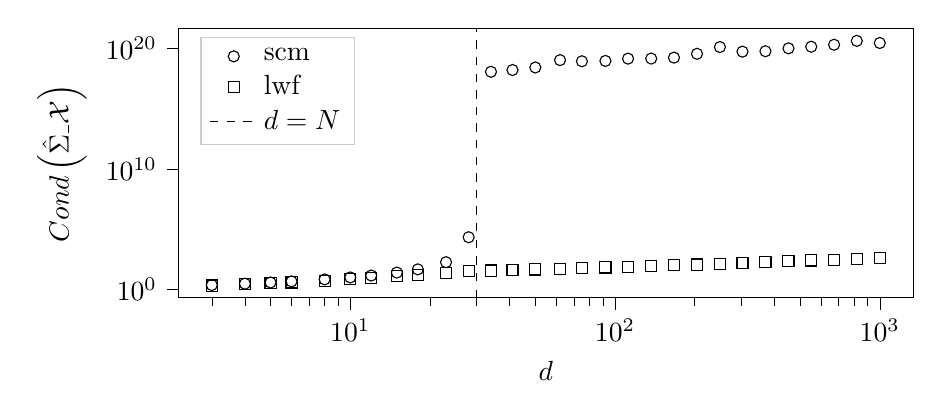
\begin{tikzpicture}

\definecolor{darkgray176}{RGB}{176,176,176}
\definecolor{lightgray204}{RGB}{204,204,204}

\begin{axis}[
width=0.9\textwidth,
height=5cm,
legend cell align={left},
legend style={
  fill opacity=0.8,
  draw opacity=1,
  text opacity=1,
  at={(0.03,0.97)},
  anchor=north west,
  draw=lightgray204
},
log basis x={10},
log basis y={10},
tick align=outside,
tick pos=left,
x grid style={darkgray176},
xlabel={\(\displaystyle d\)},
xmin=2.2437647322819, xmax=1337.03857487278,
xmode=log,
xtick style={color=black},
y grid style={darkgray176},
ylabel={\(\displaystyle \operatorname{Cond}\left(\hat{\boldsymbol{\Sigma}}\_\mathcal{X}\right)\)},
ymin=0.201647470461523, ymax=4.15155099642133e+21,
ymode=log,
ytick style={color=black}
]
\addplot [draw=black, mark=o, only marks]
table{%
x  y
3 2.30128721449648
4 2.98980176023402
5 3.74725148388153
6 4.6273062005471
8 6.80978228176998
10 9.85053405764688
12 14.1914261593259
15 24.8541084638651
18 45.8675117285121
23 181.624000745188
28 21118.5385109043
34 1.09423163871398e+18
41 1.54003337498655e+18
50 2.50285206785319e+18
62 1.02082277017018e+19
75 8.1696391406987e+18
92 8.78584488032868e+18
112 1.35351469825842e+19
137 1.37578020462997e+19
167 1.64652490481264e+19
204 3.4004576745693e+19
249 1.23230576162333e+20
303 5.12553978317069e+19
370 5.56209683272156e+19
452 9.65397291811529e+19
551 1.31245394055025e+20
672 1.91723632520982e+20
819 4.01749210190887e+20
1000 2.688261444791e+20
};
\addlegendentry{scm}
\addplot [draw=black, mark=square, only marks]
table{%
x  y
3 2.08376204777757
4 2.61314454230052
5 3.16591813272362
6 3.77123844164103
8 5.13511623080211
10 6.77168486719545
12 8.71032931589613
15 12.2362812865225
18 16.4991664311053
23 24.8178442526396
28 32.3101652848017
34 36.5636052780593
41 40.5410850707775
50 45.4758482161132
62 51.6716281093582
75 58.1312729983865
92 66.2939693288016
112 75.574506526652
137 86.8340390332717
167 99.9506811186795
204 115.670898107282
249 134.305665661733
303 156.108872096172
370 182.65218162239
452 214.359032952562
551 251.955200483623
672 297.023053266565
819 350.971958998932
1000 416.434315421376
};
\addlegendentry{lwf}
\addplot [semithick, black, dashed]
table {%
30 0.201647470461523
30 4.15155099642133e+21
};
\addlegendentry{$d=N$}
\end{axis}

\end{tikzpicture}

      \end{center}
  \provLwfcondQR[.5cm]
  \caption{\'Evolution du conditionnement de la matrice estimée par SCM et Ledoit-Wolf pour une taille croissante de variables $\Nvar$ avec $\Nobs=30$, $\coefledoitwolf=0.1$ et $\targetledoitwolf=\Id{\Nvar}$. Les marqueurs indique la moyenne du conditionnement sur 50 tirages de monte-carlo. \provLwfcond}
  \label{fig:context-estimation-condlwf}
\end{figure}



Nous nous sommes intéressés ici uniquement à la régularisation de Ledoit-Wolf car elle nous sera utile par la suite mais plusieurs approches alternatives existent. Pour un état de l'art sur le sujet, on peut se référer par exemple à \sidecite{Mohsen_Pourahmadi_2013}.


\section{Distribution de probabilités à paramètre de covariance}
\label{sec:context-distributions}

Considérons maintenant un apriori supplémentaire sur nos variables aléatoires: la connaissance de la d.d.p $\p{\Variable}$ qui régit leur comportement et essayons de préciser la notion de covariance comme un paramètre de la distribution puis intéressons nous à l'estimation de celle-ci à l'aide de la connaissance supplémentaire que l'on introduit. Nous verrons alors que la scm donnée en \cref{eq:context-estimation-covariance}, obtenue jusqu'ici sans aucun modèle, réapparait naturellement comme l'estimateur au sens du mle sous hypothèse gaussienne. Mais nous verrons également que ce résultat est fragile: dès que l'on s'écarte de ce modèle, notamment vers des distributions à queues lourdes, il faut lui substituer toute une famille d'estimateurs dits robustes.

\subsection{Distribution gaussienne}
\label{subsec:context-distributions-gaussian}

La première distribution que l'on considère, de par sa simplicité et son omniprésence, est la gaussienne dont la d.d.p est donnée par:
\begin{equation}
  \ddp{\Variable}(\x; \param) = (2\pi)^{-\Nvar/2}\Det(\MCov_\Variable)^{-1/2}\exp\left\{ -\frac{1}{2}\quadratic{(\x-\Vmoy_\Variable)}{\MCov_\Variable} \right\},
  \label{eq:context-definition-gaussian}
\end{equation}

où $\param = (\Vmoy_\Variable, \MCov_\Variable)$ sont les paramètres de la distribution. On notera que la matrice de covariance doit être définie positive pour que la d.d.p soit bien définie\footnote{Ce sera par ailleurs le cas pour toutes les distributions que l'on considérera par la suite. On notera $\SPD{\Nvar}$ l'ensemble des matrices symmétriques définies positives de taille $\Nvar\times\Nvar$, dont la structure de cône a été évoquée en \cref{fig:context-figure-spdcone}.}.

\begin{definition}[{Vecteur aléatoire gaussien}]
  On dit qu'une variable aléatoire $\Variable\in\R^\Nvar$ suit une distribution gaussienne multivariée de moyenne $\Vmoy_\Variable$ et de matrice de covariance $\MCov_\Variable$, et on note $\Variable\sim\gaussian(\Vmoy_\Variable, \MCov_\Variable)$ si sa d.d.p est donnée par \cref{eq:context-definition-gaussian}.
\end{definition}

\begin{figure}[h]
  \begin{center}
    % This file was created with matplot2tikz v0.5.3.
\begin{tikzpicture}

\definecolor{crimson2143940}{RGB}{214,39,40}
\definecolor{darkgray176}{RGB}{176,176,176}
\definecolor{darkorange25512714}{RGB}{255,127,14}
\definecolor{steelblue31119180}{RGB}{31,119,180}

\begin{groupplot}[group style={group size=3 by 1}]
\nextgroupplot[
width=0.33\textwidth,
height=4.5cm,
tick align=outside,
tick pos=left,
title={\(\displaystyle \mathbf{\Sigma} = \mathbf{I}_2\)},
x grid style={darkgray176},
xlabel={\(\displaystyle x_1\)},
xmin=-4.47885268011397, xmax=4.47885268011397,
xtick style={color=black},
y grid style={darkgray176},
ylabel={\(\displaystyle x_2\)},
ymin=-4.47885268011397, ymax=4.47885268011397,
ytick style={color=black}
]
\addplot [draw=steelblue31119180, mark=o, only marks]
table{%
x  y
0.304717079754431 -1.0399841062405
0.750451195806457 0.940564716391214
-1.95103518865384 -1.30217950686232
0.127840403167285 -0.316242592343582
-0.0168011575042888 -0.85304392757358
0.879397974862829 0.777791935428948
0.066030697561216 1.12724120696803
0.467509342252046 -0.859292462883238
0.368750784082499 -0.958882600828999
0.878450301307273 -0.0499259109862529
-0.184862363545261 -0.680929544403941
1.22254133867403 -0.154529482068802
-0.428327822163107 -0.35213355048823
0.532309185553349 0.365444064364078
0.412732611595988 0.430821003007883
2.14164760087046 -0.406415016384616
-0.512242729071537 -0.813772728247878
0.615979422575496 1.12897229272089
-0.113947457654875 -0.840156476962528
-0.82448121569124 0.650592787824701
0.743254171203442 0.543154268305195
-0.665509707288694 0.23216132306672
0.116685809140728 0.218688596729013
0.87142877794819 0.223595548774682
0.678913563071895 0.0675790694888915
0.289119398689984 0.63128822583854
-1.45715581985567 -0.319671216357301
-0.470372654292796 -0.638877848243342
-0.275142251226684 1.4949413112344
-0.865831115693243 0.968278354591481
-1.6828697716158 -0.334885029985775
0.162753065105006 0.586222331359278
0.711226579792855 0.793347235199925
-0.348725072248438 -0.462351792664567
0.857975881257154 -0.191304324881615
-1.27568632333792 -1.13328721400348
-0.919452286001611 0.497160744053764
0.142425736070565 0.690485354067768
-0.427252646336534 0.158539691076714
0.625590393967337 -0.309346539720238
0.456775237557411 -0.661925941066651
-0.363053846565072 -0.381737893998329
-1.19583964558904 0.486972480785582
-0.469402340202724 0.0124941187276874
0.480746658905909 0.446531176029944
0.665385108972786 -0.0984854845094236
-0.423298312044154 -0.0797182109063991
-1.68733443395803 -1.44711247242309
-1.3226996123544 -0.997246827601482
0.399774226723437 -0.905479055360061
};
\path [draw=darkorange25512714, line width=0.48pt]
(axis cs:-0.303080256549066,-3.01968575529092)
--(axis cs:-0.280629867175061,-3.02191401086988)
--(axis cs:-0.258179477801057,-3.02395794369153)
--(axis cs:-0.235729088427052,-3.02582071989127)
--(axis cs:-0.213278699053046,-3.02750521409603)
--(axis cs:-0.190828309679041,-3.02901401681795)
--(axis cs:-0.168377920305037,-3.03034944109444)
--(axis cs:-0.145927530931032,-3.03151352839874)
--(axis cs:-0.123477141557027,-3.03250805384192)
--(axis cs:-0.101026752183023,-3.03333453068493)
--(axis cs:-0.0785763628090175,-3.0339942141768)
--(axis cs:-0.0561259734350124,-3.03448810473263)
--(axis cs:-0.0336755840610072,-3.03481695046254)
--(axis cs:-0.011225194687003,-3.03498124906064)
--(axis cs:0.0112251946870021,-3.03498124906064)
--(axis cs:0.0336755840610072,-3.03481695046254)
--(axis cs:0.0561259734350124,-3.03448810473263)
--(axis cs:0.0785763628090166,-3.0339942141768)
--(axis cs:0.101026752183022,-3.03333453068493)
--(axis cs:0.123477141557027,-3.03250805384192)
--(axis cs:0.145927530931031,-3.03151352839874)
--(axis cs:0.168377920305036,-3.03034944109444)
--(axis cs:0.190828309679041,-3.02901401681795)
--(axis cs:0.213278699053046,-3.02750521409603)
--(axis cs:0.235729088427051,-3.02582071989127)
--(axis cs:0.258179477801056,-3.02395794369153)
--(axis cs:0.280629867175061,-3.02191401086988)
--(axis cs:0.303080256549066,-3.01968575529092)
--(axis cs:0.304094197591445,-3.01957737080366)
--(axis cs:0.32553064592307,-3.01740486550425)
--(axis cs:0.347981035297075,-3.01494997990384)
--(axis cs:0.37043142467108,-3.01231089739939)
--(axis cs:0.392881814045086,-3.00948345481859)
--(axis cs:0.41533220341909,-3.00646316813445)
--(axis cs:0.437782592793095,-3.00324522062143)
--(axis cs:0.4602329821671,-2.99982445006407)
--(axis cs:0.476965255842626,-2.99712698142965)
--(axis cs:0.482683371541104,-2.99624940834703)
--(axis cs:0.505133760915109,-2.99262912399509)
--(axis cs:0.527584150289115,-2.98880111332288)
--(axis cs:0.55003453966312,-2.98475907199707)
--(axis cs:0.572484929037124,-2.98049629491202)
--(axis cs:0.594935318411129,-2.97600565770626)
--(axis cs:0.60131076978327,-2.97467659205565)
--(axis cs:0.617385707785134,-2.97147496671274)
--(axis cs:0.639836097159139,-2.96679126779221)
--(axis cs:0.662286486533143,-2.96187010590752)
--(axis cs:0.684736875907148,-2.95670298616389)
--(axis cs:0.70332347377446,-2.95222620268164)
--(axis cs:0.707187265281154,-2.95133477737463)
--(axis cs:0.729637654655158,-2.94597226146247)
--(axis cs:0.752088044029163,-2.94035083051952)
--(axis cs:0.774538433403168,-2.93446042650009)
--(axis cs:0.791656053110558,-2.92977581330764)
--(axis cs:0.796988822777173,-2.92837426509562)
--(axis cs:0.819439212151178,-2.92227811822303)
--(axis cs:0.841889601525183,-2.91589629781146)
--(axis cs:0.864339990899188,-2.90921693110969)
--(axis cs:0.870503070771815,-2.90732542393363)
--(axis cs:0.886790380273193,-2.90251254925302)
--(axis cs:0.909240769647197,-2.89560865330928)
--(axis cs:0.931691159021202,-2.88838621825588)
--(axis cs:0.94224329811802,-2.88487503455963)
--(axis cs:0.954141548395207,-2.8810552153107)
--(axis cs:0.976591937769212,-2.87359056967625)
--(axis cs:0.999042327143217,-2.86578300364184)
--(axis cs:1.00839867685656,-2.86242464518562)
--(axis cs:1.02149271651722,-2.8578805962979)
--(axis cs:1.04394310589123,-2.84980786349028)
--(axis cs:1.06639349526523,-2.84136403193242)
--(axis cs:1.06999865574602,-2.83997425581162)
--(axis cs:1.08884388463924,-2.83293587288789)
--(axis cs:1.11129427401324,-2.82419818021901)
--(axis cs:1.12779681080737,-2.81752386643761)
--(axis cs:1.13374466338725,-2.8151895949597)
--(axis cs:1.15619505276125,-2.80613953008305)
--(axis cs:1.17864544213526,-2.79666934802634)
--(axis cs:1.18234211208092,-2.79507347706361)
--(axis cs:1.20109583150926,-2.78720096877972)
--(axis cs:1.22354622088327,-2.77737920083769)
--(axis cs:1.23408562692089,-2.7726230876896)
--(axis cs:1.24599661025727,-2.76738820214624)
--(axis cs:1.26844699963128,-2.7571894367993)
--(axis cs:1.28334049667569,-2.7501726983156)
--(axis cs:1.29089738900528,-2.74669981053274)
--(axis cs:1.31334777837928,-2.736095695509)
--(axis cs:1.33039157113298,-2.72772230894159)
--(axis cs:1.33579816775329,-2.72512721177175)
--(axis cs:1.3582485571273,-2.7140862165202)
--(axis cs:1.37547226364472,-2.70527191956759)
--(axis cs:1.3806989465013,-2.70265453038816)
--(axis cs:1.4031493358753,-2.69114166688832)
--(axis cs:1.41877291940469,-2.68282153019358)
--(axis cs:1.42559972524931,-2.67925837053454)
--(axis cs:1.44805011462331,-2.66723486834396)
--(axis cs:1.46044747423765,-2.66037114081958)
--(axis cs:1.47050050399732,-2.65490748835775)
--(axis cs:1.49295089337132,-2.64233041894764)
--(axis cs:1.50061876167187,-2.63792075144557)
--(axis cs:1.51540128274533,-2.6295623576199)
--(axis cs:1.53785167211933,-2.61638420209376)
--(axis cs:1.53938274037041,-2.61547036207157)
--(axis cs:1.56030206149334,-2.60317462036365)
--(axis cs:1.57693732165286,-2.59301997269756)
--(axis cs:1.58275245086734,-2.58952055159595)
--(axis cs:1.60520284024135,-2.5756864121794)
--(axis cs:1.6132881562023,-2.57056958332356)
--(axis cs:1.62765322961535,-2.56159317024227)
--(axis cs:1.64848018108028,-2.54811919394955)
--(axis cs:1.65010361898936,-2.54708102499448)
--(axis cs:1.67255400836336,-2.53248446105125)
--(axis cs:1.68272583016827,-2.52566880457555)
--(axis cs:1.69500439773737,-2.51752345705958)
--(axis cs:1.71589661812331,-2.50321841520154)
--(axis cs:1.71745478711137,-2.50216100266532)
--(axis cs:1.73990517648538,-2.48667937998091)
--(axis cs:1.74824836946447,-2.48076802582754)
--(axis cs:1.76235556585938,-2.47084571822937)
--(axis cs:1.77966505548568,-2.45831763645353)
--(axis cs:1.78480595523339,-2.45461994724383)
--(axis cs:1.80725634460739,-2.43811138498148)
--(axis cs:1.81025516856099,-2.43586724707953)
--(axis cs:1.8297067339814,-2.42137828394308)
--(axis cs:1.84012457862108,-2.41341685770553)
--(axis cs:1.8521571233554,-2.40425402671029)
--(axis cs:1.86918439697455,-2.39096646833152)
--(axis cs:1.87460751272941,-2.38674480254565)
--(axis cs:1.89705790210341,-2.36887050117173)
--(axis cs:1.8974975732177,-2.36851607895751)
--(axis cs:1.91950829147742,-2.35078817285462)
--(axis cs:1.9252467926298,-2.34606568958351)
--(axis cs:1.94195868085142,-2.3323092870542)
--(axis cs:1.95230741903537,-2.32361530020951)
--(axis cs:1.96440907022543,-2.31343497762009)
--(axis cs:1.97871687318406,-2.3011649108355)
--(axis cs:1.98685945959943,-2.29416487283479)
--(axis cs:2.00450915173516,-2.2787145214615)
--(axis cs:2.00930984897344,-2.27449707953444)
--(axis cs:2.02971507878362,-2.25626413208749)
--(axis cs:2.03176023834744,-2.25442815816847)
--(axis cs:2.05421062772145,-2.23395878948756)
--(axis cs:2.05436797228249,-2.23381374271349)
--(axis cs:2.07666101709545,-2.21313378006209)
--(axis cs:2.07854284029527,-2.21136335333948)
--(axis cs:2.09911140646946,-2.19186898047402)
--(axis cs:2.1021901309241,-2.18891296396548)
--(axis cs:2.12156179584346,-2.17015472371044)
--(axis cs:2.12532979011687,-2.16646257459147)
--(axis cs:2.14401218521747,-2.14797948365909)
--(axis cs:2.14797948365909,-2.14401218521747)
--(axis cs:2.16646257459147,-2.12532979011687)
--(axis cs:2.17015472371043,-2.12156179584346)
--(axis cs:2.18891296396548,-2.1021901309241)
--(axis cs:2.19186898047402,-2.09911140646946)
--(axis cs:2.21136335333948,-2.07854284029527)
--(axis cs:2.21313378006209,-2.07666101709545)
--(axis cs:2.23381374271348,-2.05436797228249)
--(axis cs:2.23395878948756,-2.05421062772145)
--(axis cs:2.25442815816847,-2.03176023834744)
--(axis cs:2.25626413208749,-2.02971507878362)
--(axis cs:2.27449707953444,-2.00930984897344)
--(axis cs:2.2787145214615,-2.00450915173516)
--(axis cs:2.29416487283479,-1.98685945959943)
--(axis cs:2.3011649108355,-1.97871687318406)
--(axis cs:2.31343497762009,-1.96440907022543)
--(axis cs:2.3236153002095,-1.95230741903537)
--(axis cs:2.3323092870542,-1.94195868085142)
--(axis cs:2.34606568958351,-1.92524679262981)
--(axis cs:2.35078817285462,-1.91950829147742)
--(axis cs:2.36851607895751,-1.8974975732177)
--(axis cs:2.36887050117173,-1.89705790210341)
--(axis cs:2.38674480254565,-1.87460751272941)
--(axis cs:2.39096646833152,-1.86918439697455)
--(axis cs:2.40425402671029,-1.8521571233554)
--(axis cs:2.41341685770552,-1.84012457862108)
--(axis cs:2.42137828394308,-1.8297067339814)
--(axis cs:2.43586724707953,-1.810255168561)
--(axis cs:2.43811138498148,-1.80725634460739)
--(axis cs:2.45461994724383,-1.78480595523339)
--(axis cs:2.45831763645353,-1.77966505548568)
--(axis cs:2.47084571822937,-1.76235556585938)
--(axis cs:2.48076802582754,-1.74824836946447)
--(axis cs:2.48667937998091,-1.73990517648538)
--(axis cs:2.50216100266532,-1.71745478711137)
--(axis cs:2.50321841520154,-1.71589661812331)
--(axis cs:2.51752345705958,-1.69500439773737)
--(axis cs:2.52566880457555,-1.68272583016827)
--(axis cs:2.53248446105125,-1.67255400836336)
--(axis cs:2.54708102499448,-1.65010361898936)
--(axis cs:2.54811919394955,-1.64848018108028)
--(axis cs:2.56159317024227,-1.62765322961535)
--(axis cs:2.57056958332356,-1.6132881562023)
--(axis cs:2.5756864121794,-1.60520284024135)
--(axis cs:2.58952055159595,-1.58275245086734)
--(axis cs:2.59301997269756,-1.57693732165286)
--(axis cs:2.60317462036365,-1.56030206149334)
--(axis cs:2.61547036207157,-1.53938274037041)
--(axis cs:2.61638420209376,-1.53785167211933)
--(axis cs:2.6295623576199,-1.51540128274533)
--(axis cs:2.63792075144557,-1.50061876167187)
--(axis cs:2.64233041894764,-1.49295089337132)
--(axis cs:2.65490748835775,-1.47050050399732)
--(axis cs:2.66037114081958,-1.46044747423765)
--(axis cs:2.66723486834396,-1.44805011462332)
--(axis cs:2.67925837053454,-1.42559972524931)
--(axis cs:2.68282153019358,-1.41877291940469)
--(axis cs:2.69114166688832,-1.40314933587531)
--(axis cs:2.70265453038816,-1.3806989465013)
--(axis cs:2.70527191956759,-1.37547226364472)
--(axis cs:2.7140862165202,-1.3582485571273)
--(axis cs:2.72512721177175,-1.33579816775329)
--(axis cs:2.72772230894159,-1.33039157113298)
--(axis cs:2.736095695509,-1.31334777837929)
--(axis cs:2.74669981053274,-1.29089738900528)
--(axis cs:2.7501726983156,-1.28334049667569)
--(axis cs:2.7571894367993,-1.26844699963128)
--(axis cs:2.76738820214624,-1.24599661025727)
--(axis cs:2.7726230876896,-1.23408562692089)
--(axis cs:2.77737920083769,-1.22354622088327)
--(axis cs:2.78720096877972,-1.20109583150926)
--(axis cs:2.79507347706361,-1.18234211208092)
--(axis cs:2.79666934802634,-1.17864544213526)
--(axis cs:2.80613953008305,-1.15619505276125)
--(axis cs:2.8151895949597,-1.13374466338725)
--(axis cs:2.81752386643761,-1.12779681080738)
--(axis cs:2.82419818021901,-1.11129427401324)
--(axis cs:2.83293587288789,-1.08884388463924)
--(axis cs:2.83997425581162,-1.06999865574602)
--(axis cs:2.84136403193242,-1.06639349526523)
--(axis cs:2.84980786349028,-1.04394310589123)
--(axis cs:2.8578805962979,-1.02149271651722)
--(axis cs:2.86242464518562,-1.00839867685656)
--(axis cs:2.86578300364184,-0.999042327143218)
--(axis cs:2.87359056967625,-0.976591937769212)
--(axis cs:2.8810552153107,-0.954141548395208)
--(axis cs:2.88487503455963,-0.94224329811802)
--(axis cs:2.88838621825588,-0.931691159021203)
--(axis cs:2.89560865330928,-0.909240769647198)
--(axis cs:2.90251254925302,-0.886790380273193)
--(axis cs:2.90732542393363,-0.870503070771818)
--(axis cs:2.90921693110969,-0.864339990899188)
--(axis cs:2.91589629781146,-0.841889601525183)
--(axis cs:2.92227811822303,-0.819439212151178)
--(axis cs:2.92837426509562,-0.796988822777173)
--(axis cs:2.92977581330764,-0.791656053110559)
--(axis cs:2.93446042650009,-0.774538433403169)
--(axis cs:2.94035083051952,-0.752088044029164)
--(axis cs:2.94597226146247,-0.729637654655159)
--(axis cs:2.95133477737463,-0.707187265281154)
--(axis cs:2.95222620268164,-0.703323473774459)
--(axis cs:2.95670298616389,-0.684736875907149)
--(axis cs:2.96187010590752,-0.662286486533144)
--(axis cs:2.96679126779221,-0.639836097159139)
--(axis cs:2.97147496671274,-0.617385707785135)
--(axis cs:2.97467659205565,-0.60131076978327)
--(axis cs:2.97600565770626,-0.594935318411129)
--(axis cs:2.98049629491202,-0.572484929037125)
--(axis cs:2.98475907199707,-0.55003453966312)
--(axis cs:2.98880111332288,-0.527584150289115)
--(axis cs:2.99262912399508,-0.50513376091511)
--(axis cs:2.99624940834703,-0.482683371541105)
--(axis cs:2.99712698142965,-0.476965255842631)
--(axis cs:2.99982445006407,-0.4602329821671)
--(axis cs:3.00324522062143,-0.437782592793096)
--(axis cs:3.00646316813445,-0.415332203419091)
--(axis cs:3.00948345481859,-0.392881814045086)
--(axis cs:3.01231089739939,-0.37043142467108)
--(axis cs:3.01494997990384,-0.347981035297076)
--(axis cs:3.01740486550425,-0.325530645923071)
--(axis cs:3.01957737080366,-0.304094197591451)
--(axis cs:3.01968575529092,-0.303080256549066)
--(axis cs:3.02191401086988,-0.280629867175061)
--(axis cs:3.02395794369153,-0.258179477801057)
--(axis cs:3.02582071989127,-0.235729088427052)
--(axis cs:3.02750521409604,-0.213278699053046)
--(axis cs:3.02901401681795,-0.190828309679041)
--(axis cs:3.03034944109444,-0.168377920305037)
--(axis cs:3.03151352839874,-0.145927530931032)
--(axis cs:3.03250805384192,-0.123477141557027)
--(axis cs:3.03333453068493,-0.101026752183023)
--(axis cs:3.0339942141768,-0.0785763628090175)
--(axis cs:3.03448810473263,-0.0561259734350124)
--(axis cs:3.03481695046254,-0.0336755840610072)
--(axis cs:3.03498124906064,-0.011225194687003)
--(axis cs:3.03498124906064,0.0112251946870021)
--(axis cs:3.03481695046254,0.0336755840610072)
--(axis cs:3.03448810473263,0.0561259734350124)
--(axis cs:3.0339942141768,0.0785763628090166)
--(axis cs:3.03333453068493,0.101026752183022)
--(axis cs:3.03250805384192,0.123477141557027)
--(axis cs:3.03151352839874,0.145927530931031)
--(axis cs:3.03034944109444,0.168377920305036)
--(axis cs:3.02901401681795,0.190828309679041)
--(axis cs:3.02750521409604,0.213278699053046)
--(axis cs:3.02582071989127,0.235729088427051)
--(axis cs:3.02395794369153,0.258179477801056)
--(axis cs:3.02191401086988,0.280629867175061)
--(axis cs:3.01968575529092,0.303080256549066)
--(axis cs:3.01957737080366,0.304094197591451)
--(axis cs:3.01740486550425,0.32553064592307)
--(axis cs:3.01494997990384,0.347981035297075)
--(axis cs:3.01231089739939,0.37043142467108)
--(axis cs:3.00948345481859,0.392881814045086)
--(axis cs:3.00646316813445,0.41533220341909)
--(axis cs:3.00324522062143,0.437782592793095)
--(axis cs:2.99982445006407,0.4602329821671)
--(axis cs:2.99712698142965,0.476965255842631)
--(axis cs:2.99624940834703,0.482683371541104)
--(axis cs:2.99262912399508,0.505133760915109)
--(axis cs:2.98880111332288,0.527584150289115)
--(axis cs:2.98475907199707,0.55003453966312)
--(axis cs:2.98049629491202,0.572484929037124)
--(axis cs:2.97600565770626,0.594935318411129)
--(axis cs:2.97467659205565,0.60131076978327)
--(axis cs:2.97147496671274,0.617385707785134)
--(axis cs:2.96679126779221,0.639836097159139)
--(axis cs:2.96187010590752,0.662286486533143)
--(axis cs:2.95670298616389,0.684736875907148)
--(axis cs:2.95222620268164,0.70332347377446)
--(axis cs:2.95133477737463,0.707187265281154)
--(axis cs:2.94597226146247,0.729637654655158)
--(axis cs:2.94035083051952,0.752088044029163)
--(axis cs:2.93446042650009,0.774538433403168)
--(axis cs:2.92977581330764,0.791656053110559)
--(axis cs:2.92837426509562,0.796988822777173)
--(axis cs:2.92227811822303,0.819439212151178)
--(axis cs:2.91589629781146,0.841889601525183)
--(axis cs:2.90921693110969,0.864339990899188)
--(axis cs:2.90732542393363,0.870503070771818)
--(axis cs:2.90251254925302,0.886790380273193)
--(axis cs:2.89560865330928,0.909240769647197)
--(axis cs:2.88838621825588,0.931691159021202)
--(axis cs:2.88487503455963,0.942243298118021)
--(axis cs:2.8810552153107,0.954141548395207)
--(axis cs:2.87359056967625,0.976591937769212)
--(axis cs:2.86578300364184,0.999042327143217)
--(axis cs:2.86242464518562,1.00839867685656)
--(axis cs:2.8578805962979,1.02149271651722)
--(axis cs:2.84980786349028,1.04394310589123)
--(axis cs:2.84136403193242,1.06639349526523)
--(axis cs:2.83997425581162,1.06999865574602)
--(axis cs:2.83293587288789,1.08884388463924)
--(axis cs:2.82419818021901,1.11129427401324)
--(axis cs:2.81752386643761,1.12779681080738)
--(axis cs:2.8151895949597,1.13374466338725)
--(axis cs:2.80613953008305,1.15619505276125)
--(axis cs:2.79666934802634,1.17864544213526)
--(axis cs:2.79507347706361,1.18234211208092)
--(axis cs:2.78720096877972,1.20109583150926)
--(axis cs:2.77737920083769,1.22354622088327)
--(axis cs:2.7726230876896,1.23408562692089)
--(axis cs:2.76738820214624,1.24599661025727)
--(axis cs:2.7571894367993,1.26844699963128)
--(axis cs:2.7501726983156,1.28334049667569)
--(axis cs:2.74669981053274,1.29089738900528)
--(axis cs:2.736095695509,1.31334777837928)
--(axis cs:2.72772230894159,1.33039157113298)
--(axis cs:2.72512721177175,1.33579816775329)
--(axis cs:2.7140862165202,1.3582485571273)
--(axis cs:2.70527191956759,1.37547226364472)
--(axis cs:2.70265453038816,1.3806989465013)
--(axis cs:2.69114166688832,1.4031493358753)
--(axis cs:2.68282153019358,1.41877291940469)
--(axis cs:2.67925837053454,1.42559972524931)
--(axis cs:2.66723486834396,1.44805011462331)
--(axis cs:2.66037114081958,1.46044747423765)
--(axis cs:2.65490748835775,1.47050050399732)
--(axis cs:2.64233041894764,1.49295089337132)
--(axis cs:2.63792075144557,1.50061876167187)
--(axis cs:2.6295623576199,1.51540128274533)
--(axis cs:2.61638420209376,1.53785167211933)
--(axis cs:2.61547036207157,1.53938274037041)
--(axis cs:2.60317462036365,1.56030206149334)
--(axis cs:2.59301997269756,1.57693732165286)
--(axis cs:2.58952055159595,1.58275245086734)
--(axis cs:2.5756864121794,1.60520284024135)
--(axis cs:2.57056958332356,1.6132881562023)
--(axis cs:2.56159317024227,1.62765322961535)
--(axis cs:2.54811919394955,1.64848018108028)
--(axis cs:2.54708102499448,1.65010361898936)
--(axis cs:2.53248446105125,1.67255400836336)
--(axis cs:2.52566880457555,1.68272583016827)
--(axis cs:2.51752345705958,1.69500439773737)
--(axis cs:2.50321841520154,1.71589661812331)
--(axis cs:2.50216100266532,1.71745478711137)
--(axis cs:2.48667937998091,1.73990517648538)
--(axis cs:2.48076802582754,1.74824836946447)
--(axis cs:2.47084571822937,1.76235556585938)
--(axis cs:2.45831763645353,1.77966505548568)
--(axis cs:2.45461994724383,1.78480595523339)
--(axis cs:2.43811138498148,1.80725634460739)
--(axis cs:2.43586724707953,1.810255168561)
--(axis cs:2.42137828394308,1.8297067339814)
--(axis cs:2.41341685770552,1.84012457862108)
--(axis cs:2.40425402671029,1.8521571233554)
--(axis cs:2.39096646833152,1.86918439697455)
--(axis cs:2.38674480254565,1.87460751272941)
--(axis cs:2.36887050117173,1.89705790210341)
--(axis cs:2.36851607895751,1.8974975732177)
--(axis cs:2.35078817285462,1.91950829147742)
--(axis cs:2.34606568958351,1.92524679262981)
--(axis cs:2.3323092870542,1.94195868085142)
--(axis cs:2.3236153002095,1.95230741903537)
--(axis cs:2.31343497762009,1.96440907022543)
--(axis cs:2.3011649108355,1.97871687318406)
--(axis cs:2.29416487283479,1.98685945959943)
--(axis cs:2.2787145214615,2.00450915173516)
--(axis cs:2.27449707953444,2.00930984897344)
--(axis cs:2.25626413208749,2.02971507878362)
--(axis cs:2.25442815816847,2.03176023834744)
--(axis cs:2.23395878948756,2.05421062772145)
--(axis cs:2.23381374271348,2.05436797228249)
--(axis cs:2.21313378006209,2.07666101709545)
--(axis cs:2.21136335333948,2.07854284029527)
--(axis cs:2.19186898047402,2.09911140646946)
--(axis cs:2.18891296396548,2.1021901309241)
--(axis cs:2.17015472371043,2.12156179584346)
--(axis cs:2.16646257459147,2.12532979011687)
--(axis cs:2.14797948365909,2.14401218521747)
--(axis cs:2.14401218521747,2.14797948365909)
--(axis cs:2.12532979011687,2.16646257459147)
--(axis cs:2.12156179584346,2.17015472371044)
--(axis cs:2.1021901309241,2.18891296396548)
--(axis cs:2.09911140646946,2.19186898047402)
--(axis cs:2.07854284029527,2.21136335333948)
--(axis cs:2.07666101709545,2.21313378006209)
--(axis cs:2.05436797228249,2.23381374271348)
--(axis cs:2.05421062772145,2.23395878948756)
--(axis cs:2.03176023834744,2.25442815816847)
--(axis cs:2.02971507878362,2.25626413208749)
--(axis cs:2.00930984897344,2.27449707953444)
--(axis cs:2.00450915173516,2.2787145214615)
--(axis cs:1.98685945959943,2.29416487283479)
--(axis cs:1.97871687318406,2.3011649108355)
--(axis cs:1.96440907022543,2.31343497762009)
--(axis cs:1.95230741903537,2.3236153002095)
--(axis cs:1.94195868085142,2.3323092870542)
--(axis cs:1.92524679262981,2.34606568958351)
--(axis cs:1.91950829147742,2.35078817285462)
--(axis cs:1.8974975732177,2.36851607895751)
--(axis cs:1.89705790210341,2.36887050117173)
--(axis cs:1.87460751272941,2.38674480254565)
--(axis cs:1.86918439697455,2.39096646833152)
--(axis cs:1.8521571233554,2.40425402671029)
--(axis cs:1.84012457862108,2.41341685770552)
--(axis cs:1.8297067339814,2.42137828394308)
--(axis cs:1.810255168561,2.43586724707953)
--(axis cs:1.80725634460739,2.43811138498148)
--(axis cs:1.78480595523339,2.45461994724383)
--(axis cs:1.77966505548568,2.45831763645353)
--(axis cs:1.76235556585938,2.47084571822937)
--(axis cs:1.74824836946447,2.48076802582754)
--(axis cs:1.73990517648538,2.48667937998091)
--(axis cs:1.71745478711137,2.50216100266532)
--(axis cs:1.71589661812331,2.50321841520154)
--(axis cs:1.69500439773737,2.51752345705958)
--(axis cs:1.68272583016827,2.52566880457555)
--(axis cs:1.67255400836336,2.53248446105125)
--(axis cs:1.65010361898936,2.54708102499448)
--(axis cs:1.64848018108028,2.54811919394955)
--(axis cs:1.62765322961535,2.56159317024227)
--(axis cs:1.6132881562023,2.57056958332356)
--(axis cs:1.60520284024135,2.5756864121794)
--(axis cs:1.58275245086734,2.58952055159595)
--(axis cs:1.57693732165286,2.59301997269756)
--(axis cs:1.56030206149334,2.60317462036365)
--(axis cs:1.53938274037041,2.61547036207157)
--(axis cs:1.53785167211933,2.61638420209376)
--(axis cs:1.51540128274533,2.6295623576199)
--(axis cs:1.50061876167187,2.63792075144557)
--(axis cs:1.49295089337132,2.64233041894764)
--(axis cs:1.47050050399732,2.65490748835775)
--(axis cs:1.46044747423765,2.66037114081958)
--(axis cs:1.44805011462331,2.66723486834396)
--(axis cs:1.42559972524931,2.67925837053454)
--(axis cs:1.41877291940469,2.68282153019358)
--(axis cs:1.4031493358753,2.69114166688832)
--(axis cs:1.3806989465013,2.70265453038816)
--(axis cs:1.37547226364472,2.70527191956759)
--(axis cs:1.3582485571273,2.7140862165202)
--(axis cs:1.33579816775329,2.72512721177175)
--(axis cs:1.33039157113298,2.72772230894159)
--(axis cs:1.31334777837928,2.736095695509)
--(axis cs:1.29089738900528,2.74669981053274)
--(axis cs:1.28334049667569,2.7501726983156)
--(axis cs:1.26844699963128,2.7571894367993)
--(axis cs:1.24599661025727,2.76738820214624)
--(axis cs:1.23408562692089,2.7726230876896)
--(axis cs:1.22354622088327,2.77737920083769)
--(axis cs:1.20109583150926,2.78720096877972)
--(axis cs:1.18234211208092,2.79507347706361)
--(axis cs:1.17864544213526,2.79666934802634)
--(axis cs:1.15619505276125,2.80613953008305)
--(axis cs:1.13374466338725,2.8151895949597)
--(axis cs:1.12779681080738,2.81752386643761)
--(axis cs:1.11129427401324,2.82419818021901)
--(axis cs:1.08884388463924,2.83293587288789)
--(axis cs:1.06999865574602,2.83997425581162)
--(axis cs:1.06639349526523,2.84136403193242)
--(axis cs:1.04394310589123,2.84980786349028)
--(axis cs:1.02149271651722,2.8578805962979)
--(axis cs:1.00839867685657,2.86242464518562)
--(axis cs:0.999042327143217,2.86578300364184)
--(axis cs:0.976591937769213,2.87359056967625)
--(axis cs:0.954141548395207,2.8810552153107)
--(axis cs:0.94224329811802,2.88487503455963)
--(axis cs:0.931691159021202,2.88838621825588)
--(axis cs:0.909240769647197,2.89560865330928)
--(axis cs:0.886790380273193,2.90251254925302)
--(axis cs:0.870503070771819,2.90732542393363)
--(axis cs:0.864339990899188,2.90921693110969)
--(axis cs:0.841889601525183,2.91589629781146)
--(axis cs:0.819439212151178,2.92227811822303)
--(axis cs:0.796988822777173,2.92837426509562)
--(axis cs:0.791656053110559,2.92977581330764)
--(axis cs:0.774538433403168,2.93446042650009)
--(axis cs:0.752088044029163,2.94035083051952)
--(axis cs:0.729637654655158,2.94597226146247)
--(axis cs:0.707187265281154,2.95133477737463)
--(axis cs:0.70332347377446,2.95222620268164)
--(axis cs:0.684736875907148,2.95670298616389)
--(axis cs:0.662286486533143,2.96187010590752)
--(axis cs:0.639836097159139,2.96679126779221)
--(axis cs:0.617385707785134,2.97147496671274)
--(axis cs:0.60131076978327,2.97467659205565)
--(axis cs:0.594935318411129,2.97600565770626)
--(axis cs:0.572484929037124,2.98049629491202)
--(axis cs:0.55003453966312,2.98475907199707)
--(axis cs:0.527584150289115,2.98880111332288)
--(axis cs:0.505133760915109,2.99262912399509)
--(axis cs:0.482683371541104,2.99624940834703)
--(axis cs:0.476965255842631,2.99712698142965)
--(axis cs:0.4602329821671,2.99982445006407)
--(axis cs:0.437782592793095,3.00324522062143)
--(axis cs:0.41533220341909,3.00646316813445)
--(axis cs:0.392881814045086,3.00948345481859)
--(axis cs:0.37043142467108,3.01231089739939)
--(axis cs:0.347981035297075,3.01494997990384)
--(axis cs:0.32553064592307,3.01740486550425)
--(axis cs:0.304094197591451,3.01957737080366)
--(axis cs:0.303080256549066,3.01968575529092)
--(axis cs:0.280629867175061,3.02191401086988)
--(axis cs:0.258179477801056,3.02395794369154)
--(axis cs:0.235729088427051,3.02582071989127)
--(axis cs:0.213278699053046,3.02750521409604)
--(axis cs:0.190828309679041,3.02901401681795)
--(axis cs:0.168377920305036,3.03034944109444)
--(axis cs:0.145927530931031,3.03151352839874)
--(axis cs:0.123477141557027,3.03250805384192)
--(axis cs:0.101026752183022,3.03333453068493)
--(axis cs:0.0785763628090166,3.0339942141768)
--(axis cs:0.0561259734350124,3.03448810473263)
--(axis cs:0.0336755840610072,3.03481695046254)
--(axis cs:0.0112251946870021,3.03498124906064)
--(axis cs:-0.011225194687003,3.03498124906064)
--(axis cs:-0.0336755840610072,3.03481695046254)
--(axis cs:-0.0561259734350124,3.03448810473263)
--(axis cs:-0.0785763628090175,3.0339942141768)
--(axis cs:-0.101026752183023,3.03333453068493)
--(axis cs:-0.123477141557027,3.03250805384192)
--(axis cs:-0.145927530931032,3.03151352839874)
--(axis cs:-0.168377920305037,3.03034944109444)
--(axis cs:-0.190828309679041,3.02901401681795)
--(axis cs:-0.213278699053046,3.02750521409604)
--(axis cs:-0.235729088427052,3.02582071989127)
--(axis cs:-0.258179477801057,3.02395794369153)
--(axis cs:-0.280629867175061,3.02191401086988)
--(axis cs:-0.303080256549066,3.01968575529092)
--(axis cs:-0.304094197591451,3.01957737080366)
--(axis cs:-0.325530645923071,3.01740486550425)
--(axis cs:-0.347981035297076,3.01494997990384)
--(axis cs:-0.37043142467108,3.01231089739939)
--(axis cs:-0.392881814045086,3.00948345481859)
--(axis cs:-0.415332203419091,3.00646316813445)
--(axis cs:-0.437782592793096,3.00324522062143)
--(axis cs:-0.4602329821671,2.99982445006407)
--(axis cs:-0.476965255842631,2.99712698142965)
--(axis cs:-0.482683371541105,2.99624940834703)
--(axis cs:-0.50513376091511,2.99262912399509)
--(axis cs:-0.527584150289115,2.98880111332288)
--(axis cs:-0.55003453966312,2.98475907199707)
--(axis cs:-0.572484929037125,2.98049629491202)
--(axis cs:-0.594935318411129,2.97600565770626)
--(axis cs:-0.60131076978327,2.97467659205565)
--(axis cs:-0.617385707785135,2.97147496671274)
--(axis cs:-0.639836097159139,2.96679126779221)
--(axis cs:-0.662286486533144,2.96187010590752)
--(axis cs:-0.684736875907149,2.95670298616389)
--(axis cs:-0.70332347377446,2.95222620268164)
--(axis cs:-0.707187265281154,2.95133477737463)
--(axis cs:-0.729637654655159,2.94597226146247)
--(axis cs:-0.752088044029164,2.94035083051952)
--(axis cs:-0.774538433403169,2.93446042650009)
--(axis cs:-0.791656053110559,2.92977581330764)
--(axis cs:-0.796988822777173,2.92837426509562)
--(axis cs:-0.819439212151178,2.92227811822303)
--(axis cs:-0.841889601525183,2.91589629781146)
--(axis cs:-0.864339990899188,2.90921693110969)
--(axis cs:-0.870503070771819,2.90732542393363)
--(axis cs:-0.886790380273193,2.90251254925302)
--(axis cs:-0.909240769647198,2.89560865330928)
--(axis cs:-0.931691159021203,2.88838621825588)
--(axis cs:-0.94224329811802,2.88487503455963)
--(axis cs:-0.954141548395208,2.8810552153107)
--(axis cs:-0.976591937769213,2.87359056967625)
--(axis cs:-0.999042327143218,2.86578300364184)
--(axis cs:-1.00839867685657,2.86242464518562)
--(axis cs:-1.02149271651722,2.8578805962979)
--(axis cs:-1.04394310589123,2.84980786349028)
--(axis cs:-1.06639349526523,2.84136403193242)
--(axis cs:-1.06999865574602,2.83997425581162)
--(axis cs:-1.08884388463924,2.83293587288789)
--(axis cs:-1.11129427401324,2.82419818021901)
--(axis cs:-1.12779681080738,2.81752386643761)
--(axis cs:-1.13374466338725,2.8151895949597)
--(axis cs:-1.15619505276125,2.80613953008305)
--(axis cs:-1.17864544213526,2.79666934802634)
--(axis cs:-1.18234211208092,2.79507347706361)
--(axis cs:-1.20109583150926,2.78720096877972)
--(axis cs:-1.22354622088327,2.77737920083769)
--(axis cs:-1.23408562692089,2.7726230876896)
--(axis cs:-1.24599661025727,2.76738820214624)
--(axis cs:-1.26844699963128,2.7571894367993)
--(axis cs:-1.28334049667569,2.7501726983156)
--(axis cs:-1.29089738900528,2.74669981053274)
--(axis cs:-1.31334777837929,2.736095695509)
--(axis cs:-1.33039157113298,2.72772230894159)
--(axis cs:-1.33579816775329,2.72512721177175)
--(axis cs:-1.3582485571273,2.7140862165202)
--(axis cs:-1.37547226364472,2.70527191956759)
--(axis cs:-1.3806989465013,2.70265453038816)
--(axis cs:-1.40314933587531,2.69114166688832)
--(axis cs:-1.41877291940469,2.68282153019358)
--(axis cs:-1.42559972524931,2.67925837053454)
--(axis cs:-1.44805011462332,2.66723486834396)
--(axis cs:-1.46044747423765,2.66037114081958)
--(axis cs:-1.47050050399732,2.65490748835775)
--(axis cs:-1.49295089337132,2.64233041894764)
--(axis cs:-1.50061876167187,2.63792075144557)
--(axis cs:-1.51540128274533,2.6295623576199)
--(axis cs:-1.53785167211933,2.61638420209376)
--(axis cs:-1.53938274037041,2.61547036207157)
--(axis cs:-1.56030206149334,2.60317462036365)
--(axis cs:-1.57693732165286,2.59301997269756)
--(axis cs:-1.58275245086734,2.58952055159595)
--(axis cs:-1.60520284024135,2.5756864121794)
--(axis cs:-1.6132881562023,2.57056958332356)
--(axis cs:-1.62765322961535,2.56159317024227)
--(axis cs:-1.64848018108028,2.54811919394955)
--(axis cs:-1.65010361898936,2.54708102499448)
--(axis cs:-1.67255400836336,2.53248446105125)
--(axis cs:-1.68272583016827,2.52566880457555)
--(axis cs:-1.69500439773737,2.51752345705958)
--(axis cs:-1.71589661812331,2.50321841520154)
--(axis cs:-1.71745478711137,2.50216100266532)
--(axis cs:-1.73990517648538,2.48667937998091)
--(axis cs:-1.74824836946447,2.48076802582754)
--(axis cs:-1.76235556585938,2.47084571822937)
--(axis cs:-1.77966505548568,2.45831763645353)
--(axis cs:-1.78480595523339,2.45461994724383)
--(axis cs:-1.80725634460739,2.43811138498148)
--(axis cs:-1.810255168561,2.43586724707953)
--(axis cs:-1.8297067339814,2.42137828394308)
--(axis cs:-1.84012457862108,2.41341685770552)
--(axis cs:-1.8521571233554,2.40425402671029)
--(axis cs:-1.86918439697455,2.39096646833152)
--(axis cs:-1.87460751272941,2.38674480254565)
--(axis cs:-1.89705790210341,2.36887050117173)
--(axis cs:-1.8974975732177,2.36851607895751)
--(axis cs:-1.91950829147742,2.35078817285462)
--(axis cs:-1.92524679262981,2.34606568958351)
--(axis cs:-1.94195868085142,2.3323092870542)
--(axis cs:-1.95230741903537,2.3236153002095)
--(axis cs:-1.96440907022543,2.31343497762009)
--(axis cs:-1.97871687318406,2.3011649108355)
--(axis cs:-1.98685945959943,2.29416487283479)
--(axis cs:-2.00450915173516,2.2787145214615)
--(axis cs:-2.00930984897344,2.27449707953444)
--(axis cs:-2.02971507878362,2.25626413208749)
--(axis cs:-2.03176023834744,2.25442815816847)
--(axis cs:-2.05421062772145,2.23395878948756)
--(axis cs:-2.05436797228249,2.23381374271348)
--(axis cs:-2.07666101709545,2.21313378006209)
--(axis cs:-2.07854284029527,2.21136335333948)
--(axis cs:-2.09911140646946,2.19186898047402)
--(axis cs:-2.1021901309241,2.18891296396548)
--(axis cs:-2.12156179584346,2.17015472371043)
--(axis cs:-2.12532979011687,2.16646257459147)
--(axis cs:-2.14401218521747,2.14797948365909)
--(axis cs:-2.14797948365909,2.14401218521747)
--(axis cs:-2.16646257459147,2.12532979011687)
--(axis cs:-2.17015472371044,2.12156179584346)
--(axis cs:-2.18891296396548,2.1021901309241)
--(axis cs:-2.19186898047402,2.09911140646946)
--(axis cs:-2.21136335333948,2.07854284029527)
--(axis cs:-2.21313378006209,2.07666101709545)
--(axis cs:-2.23381374271349,2.05436797228249)
--(axis cs:-2.23395878948756,2.05421062772145)
--(axis cs:-2.25442815816847,2.03176023834744)
--(axis cs:-2.25626413208749,2.02971507878362)
--(axis cs:-2.27449707953444,2.00930984897344)
--(axis cs:-2.2787145214615,2.00450915173516)
--(axis cs:-2.29416487283479,1.98685945959943)
--(axis cs:-2.3011649108355,1.97871687318406)
--(axis cs:-2.31343497762009,1.96440907022543)
--(axis cs:-2.32361530020951,1.95230741903537)
--(axis cs:-2.3323092870542,1.94195868085142)
--(axis cs:-2.34606568958351,1.9252467926298)
--(axis cs:-2.35078817285462,1.91950829147742)
--(axis cs:-2.36851607895751,1.8974975732177)
--(axis cs:-2.36887050117173,1.89705790210341)
--(axis cs:-2.38674480254565,1.87460751272941)
--(axis cs:-2.39096646833152,1.86918439697455)
--(axis cs:-2.40425402671029,1.8521571233554)
--(axis cs:-2.41341685770553,1.84012457862108)
--(axis cs:-2.42137828394308,1.8297067339814)
--(axis cs:-2.43586724707953,1.81025516856099)
--(axis cs:-2.43811138498148,1.80725634460739)
--(axis cs:-2.45461994724383,1.78480595523339)
--(axis cs:-2.45831763645353,1.77966505548568)
--(axis cs:-2.47084571822937,1.76235556585938)
--(axis cs:-2.48076802582754,1.74824836946447)
--(axis cs:-2.48667937998091,1.73990517648538)
--(axis cs:-2.50216100266532,1.71745478711137)
--(axis cs:-2.50321841520154,1.71589661812331)
--(axis cs:-2.51752345705958,1.69500439773737)
--(axis cs:-2.52566880457555,1.68272583016827)
--(axis cs:-2.53248446105125,1.67255400836336)
--(axis cs:-2.54708102499448,1.65010361898936)
--(axis cs:-2.54811919394955,1.64848018108028)
--(axis cs:-2.56159317024227,1.62765322961535)
--(axis cs:-2.57056958332356,1.6132881562023)
--(axis cs:-2.5756864121794,1.60520284024135)
--(axis cs:-2.58952055159595,1.58275245086734)
--(axis cs:-2.59301997269756,1.57693732165286)
--(axis cs:-2.60317462036365,1.56030206149334)
--(axis cs:-2.61547036207157,1.53938274037041)
--(axis cs:-2.61638420209376,1.53785167211933)
--(axis cs:-2.6295623576199,1.51540128274533)
--(axis cs:-2.63792075144557,1.50061876167187)
--(axis cs:-2.64233041894764,1.49295089337132)
--(axis cs:-2.65490748835775,1.47050050399732)
--(axis cs:-2.66037114081958,1.46044747423765)
--(axis cs:-2.66723486834396,1.44805011462331)
--(axis cs:-2.67925837053454,1.42559972524931)
--(axis cs:-2.68282153019358,1.41877291940469)
--(axis cs:-2.69114166688832,1.4031493358753)
--(axis cs:-2.70265453038816,1.3806989465013)
--(axis cs:-2.70527191956759,1.37547226364472)
--(axis cs:-2.7140862165202,1.3582485571273)
--(axis cs:-2.72512721177175,1.33579816775329)
--(axis cs:-2.72772230894159,1.33039157113298)
--(axis cs:-2.736095695509,1.31334777837928)
--(axis cs:-2.74669981053274,1.29089738900528)
--(axis cs:-2.7501726983156,1.28334049667569)
--(axis cs:-2.7571894367993,1.26844699963128)
--(axis cs:-2.76738820214624,1.24599661025727)
--(axis cs:-2.7726230876896,1.23408562692089)
--(axis cs:-2.77737920083769,1.22354622088327)
--(axis cs:-2.78720096877972,1.20109583150926)
--(axis cs:-2.79507347706361,1.18234211208092)
--(axis cs:-2.79666934802634,1.17864544213526)
--(axis cs:-2.80613953008305,1.15619505276125)
--(axis cs:-2.8151895949597,1.13374466338725)
--(axis cs:-2.81752386643761,1.12779681080737)
--(axis cs:-2.82419818021901,1.11129427401324)
--(axis cs:-2.83293587288789,1.08884388463924)
--(axis cs:-2.83997425581162,1.06999865574602)
--(axis cs:-2.84136403193242,1.06639349526523)
--(axis cs:-2.84980786349028,1.04394310589123)
--(axis cs:-2.8578805962979,1.02149271651722)
--(axis cs:-2.86242464518562,1.00839867685656)
--(axis cs:-2.86578300364184,0.999042327143217)
--(axis cs:-2.87359056967625,0.976591937769212)
--(axis cs:-2.8810552153107,0.954141548395207)
--(axis cs:-2.88487503455963,0.942243298118021)
--(axis cs:-2.88838621825588,0.931691159021202)
--(axis cs:-2.89560865330928,0.909240769647197)
--(axis cs:-2.90251254925302,0.886790380273193)
--(axis cs:-2.90732542393363,0.870503070771816)
--(axis cs:-2.90921693110969,0.864339990899188)
--(axis cs:-2.91589629781146,0.841889601525183)
--(axis cs:-2.92227811822303,0.819439212151178)
--(axis cs:-2.92837426509562,0.796988822777173)
--(axis cs:-2.92977581330764,0.791656053110557)
--(axis cs:-2.93446042650009,0.774538433403168)
--(axis cs:-2.94035083051952,0.752088044029163)
--(axis cs:-2.94597226146247,0.729637654655158)
--(axis cs:-2.95133477737463,0.707187265281154)
--(axis cs:-2.95222620268164,0.70332347377446)
--(axis cs:-2.95670298616389,0.684736875907148)
--(axis cs:-2.96187010590752,0.662286486533143)
--(axis cs:-2.96679126779221,0.639836097159139)
--(axis cs:-2.97147496671274,0.617385707785134)
--(axis cs:-2.97467659205565,0.60131076978327)
--(axis cs:-2.97600565770626,0.594935318411129)
--(axis cs:-2.98049629491202,0.572484929037124)
--(axis cs:-2.98475907199707,0.55003453966312)
--(axis cs:-2.98880111332288,0.527584150289115)
--(axis cs:-2.99262912399508,0.505133760915109)
--(axis cs:-2.99624940834703,0.482683371541104)
--(axis cs:-2.99712698142965,0.476965255842626)
--(axis cs:-2.99982445006407,0.4602329821671)
--(axis cs:-3.00324522062143,0.437782592793095)
--(axis cs:-3.00646316813445,0.41533220341909)
--(axis cs:-3.00948345481859,0.392881814045086)
--(axis cs:-3.01231089739939,0.37043142467108)
--(axis cs:-3.01494997990384,0.347981035297075)
--(axis cs:-3.01740486550425,0.32553064592307)
--(axis cs:-3.01957737080366,0.304094197591448)
--(axis cs:-3.01968575529092,0.303080256549066)
--(axis cs:-3.02191401086988,0.280629867175061)
--(axis cs:-3.02395794369153,0.258179477801056)
--(axis cs:-3.02582071989127,0.235729088427051)
--(axis cs:-3.02750521409603,0.213278699053046)
--(axis cs:-3.02901401681795,0.190828309679041)
--(axis cs:-3.03034944109444,0.168377920305036)
--(axis cs:-3.03151352839874,0.145927530931031)
--(axis cs:-3.03250805384192,0.123477141557027)
--(axis cs:-3.03333453068493,0.101026752183022)
--(axis cs:-3.0339942141768,0.0785763628090166)
--(axis cs:-3.03448810473263,0.0561259734350124)
--(axis cs:-3.03481695046254,0.0336755840610072)
--(axis cs:-3.03498124906064,0.0112251946870021)
--(axis cs:-3.03498124906064,-0.011225194687003)
--(axis cs:-3.03481695046254,-0.0336755840610072)
--(axis cs:-3.03448810473263,-0.0561259734350124)
--(axis cs:-3.0339942141768,-0.0785763628090175)
--(axis cs:-3.03333453068493,-0.101026752183023)
--(axis cs:-3.03250805384192,-0.123477141557027)
--(axis cs:-3.03151352839874,-0.145927530931032)
--(axis cs:-3.03034944109444,-0.168377920305037)
--(axis cs:-3.02901401681795,-0.190828309679041)
--(axis cs:-3.02750521409603,-0.213278699053046)
--(axis cs:-3.02582071989127,-0.235729088427052)
--(axis cs:-3.02395794369153,-0.258179477801057)
--(axis cs:-3.02191401086988,-0.280629867175061)
--(axis cs:-3.01968575529092,-0.303080256549066)
--(axis cs:-3.01957737080366,-0.304094197591448)
--(axis cs:-3.01740486550425,-0.325530645923071)
--(axis cs:-3.01494997990384,-0.347981035297076)
--(axis cs:-3.01231089739939,-0.37043142467108)
--(axis cs:-3.00948345481859,-0.392881814045086)
--(axis cs:-3.00646316813445,-0.415332203419091)
--(axis cs:-3.00324522062143,-0.437782592793096)
--(axis cs:-2.99982445006407,-0.4602329821671)
--(axis cs:-2.99712698142965,-0.476965255842625)
--(axis cs:-2.99624940834703,-0.482683371541105)
--(axis cs:-2.99262912399508,-0.50513376091511)
--(axis cs:-2.98880111332288,-0.527584150289115)
--(axis cs:-2.98475907199707,-0.55003453966312)
--(axis cs:-2.98049629491202,-0.572484929037125)
--(axis cs:-2.97600565770626,-0.594935318411129)
--(axis cs:-2.97467659205565,-0.60131076978327)
--(axis cs:-2.97147496671274,-0.617385707785135)
--(axis cs:-2.96679126779221,-0.639836097159139)
--(axis cs:-2.96187010590752,-0.662286486533144)
--(axis cs:-2.95670298616389,-0.684736875907149)
--(axis cs:-2.95222620268164,-0.703323473774459)
--(axis cs:-2.95133477737463,-0.707187265281154)
--(axis cs:-2.94597226146247,-0.729637654655159)
--(axis cs:-2.94035083051952,-0.752088044029164)
--(axis cs:-2.93446042650009,-0.774538433403169)
--(axis cs:-2.92977581330764,-0.791656053110557)
--(axis cs:-2.92837426509562,-0.796988822777173)
--(axis cs:-2.92227811822303,-0.819439212151178)
--(axis cs:-2.91589629781146,-0.841889601525183)
--(axis cs:-2.90921693110969,-0.864339990899188)
--(axis cs:-2.90732542393363,-0.870503070771816)
--(axis cs:-2.90251254925302,-0.886790380273193)
--(axis cs:-2.89560865330928,-0.909240769647198)
--(axis cs:-2.88838621825588,-0.931691159021203)
--(axis cs:-2.88487503455963,-0.94224329811802)
--(axis cs:-2.8810552153107,-0.954141548395208)
--(axis cs:-2.87359056967625,-0.976591937769212)
--(axis cs:-2.86578300364184,-0.999042327143218)
--(axis cs:-2.86242464518562,-1.00839867685656)
--(axis cs:-2.8578805962979,-1.02149271651722)
--(axis cs:-2.84980786349028,-1.04394310589123)
--(axis cs:-2.84136403193242,-1.06639349526523)
--(axis cs:-2.83997425581162,-1.06999865574602)
--(axis cs:-2.83293587288789,-1.08884388463924)
--(axis cs:-2.82419818021901,-1.11129427401324)
--(axis cs:-2.81752386643761,-1.12779681080737)
--(axis cs:-2.8151895949597,-1.13374466338725)
--(axis cs:-2.80613953008305,-1.15619505276125)
--(axis cs:-2.79666934802634,-1.17864544213526)
--(axis cs:-2.79507347706361,-1.18234211208092)
--(axis cs:-2.78720096877972,-1.20109583150926)
--(axis cs:-2.77737920083769,-1.22354622088327)
--(axis cs:-2.7726230876896,-1.23408562692089)
--(axis cs:-2.76738820214624,-1.24599661025727)
--(axis cs:-2.7571894367993,-1.26844699963128)
--(axis cs:-2.7501726983156,-1.28334049667569)
--(axis cs:-2.74669981053274,-1.29089738900528)
--(axis cs:-2.736095695509,-1.31334777837929)
--(axis cs:-2.72772230894159,-1.33039157113298)
--(axis cs:-2.72512721177175,-1.33579816775329)
--(axis cs:-2.7140862165202,-1.3582485571273)
--(axis cs:-2.70527191956759,-1.37547226364472)
--(axis cs:-2.70265453038816,-1.3806989465013)
--(axis cs:-2.69114166688832,-1.40314933587531)
--(axis cs:-2.68282153019358,-1.41877291940469)
--(axis cs:-2.67925837053454,-1.42559972524931)
--(axis cs:-2.66723486834396,-1.44805011462332)
--(axis cs:-2.66037114081958,-1.46044747423765)
--(axis cs:-2.65490748835775,-1.47050050399732)
--(axis cs:-2.64233041894764,-1.49295089337132)
--(axis cs:-2.63792075144557,-1.50061876167187)
--(axis cs:-2.6295623576199,-1.51540128274533)
--(axis cs:-2.61638420209376,-1.53785167211933)
--(axis cs:-2.61547036207157,-1.53938274037041)
--(axis cs:-2.60317462036365,-1.56030206149334)
--(axis cs:-2.59301997269756,-1.57693732165286)
--(axis cs:-2.58952055159595,-1.58275245086734)
--(axis cs:-2.5756864121794,-1.60520284024135)
--(axis cs:-2.57056958332356,-1.6132881562023)
--(axis cs:-2.56159317024227,-1.62765322961535)
--(axis cs:-2.54811919394955,-1.64848018108028)
--(axis cs:-2.54708102499448,-1.65010361898936)
--(axis cs:-2.53248446105125,-1.67255400836336)
--(axis cs:-2.52566880457555,-1.68272583016827)
--(axis cs:-2.51752345705958,-1.69500439773737)
--(axis cs:-2.50321841520154,-1.71589661812331)
--(axis cs:-2.50216100266532,-1.71745478711137)
--(axis cs:-2.48667937998091,-1.73990517648538)
--(axis cs:-2.48076802582754,-1.74824836946447)
--(axis cs:-2.47084571822937,-1.76235556585938)
--(axis cs:-2.45831763645353,-1.77966505548568)
--(axis cs:-2.45461994724383,-1.78480595523339)
--(axis cs:-2.43811138498148,-1.80725634460739)
--(axis cs:-2.43586724707953,-1.81025516856099)
--(axis cs:-2.42137828394308,-1.8297067339814)
--(axis cs:-2.41341685770553,-1.84012457862108)
--(axis cs:-2.40425402671029,-1.8521571233554)
--(axis cs:-2.39096646833152,-1.86918439697455)
--(axis cs:-2.38674480254565,-1.87460751272941)
--(axis cs:-2.36887050117173,-1.89705790210341)
--(axis cs:-2.36851607895752,-1.8974975732177)
--(axis cs:-2.35078817285462,-1.91950829147742)
--(axis cs:-2.34606568958351,-1.9252467926298)
--(axis cs:-2.3323092870542,-1.94195868085142)
--(axis cs:-2.32361530020951,-1.95230741903537)
--(axis cs:-2.31343497762009,-1.96440907022543)
--(axis cs:-2.3011649108355,-1.97871687318406)
--(axis cs:-2.29416487283479,-1.98685945959943)
--(axis cs:-2.2787145214615,-2.00450915173516)
--(axis cs:-2.27449707953444,-2.00930984897344)
--(axis cs:-2.25626413208749,-2.02971507878362)
--(axis cs:-2.25442815816847,-2.03176023834744)
--(axis cs:-2.23395878948756,-2.05421062772145)
--(axis cs:-2.23381374271349,-2.05436797228249)
--(axis cs:-2.21313378006209,-2.07666101709545)
--(axis cs:-2.21136335333948,-2.07854284029527)
--(axis cs:-2.19186898047402,-2.09911140646946)
--(axis cs:-2.18891296396548,-2.1021901309241)
--(axis cs:-2.17015472371043,-2.12156179584346)
--(axis cs:-2.16646257459147,-2.12532979011687)
--(axis cs:-2.14797948365909,-2.14401218521747)
--(axis cs:-2.14401218521747,-2.14797948365909)
--(axis cs:-2.12532979011687,-2.16646257459147)
--(axis cs:-2.12156179584346,-2.17015472371043)
--(axis cs:-2.1021901309241,-2.18891296396548)
--(axis cs:-2.09911140646946,-2.19186898047402)
--(axis cs:-2.07854284029527,-2.21136335333948)
--(axis cs:-2.07666101709545,-2.21313378006209)
--(axis cs:-2.05436797228249,-2.23381374271349)
--(axis cs:-2.05421062772145,-2.23395878948756)
--(axis cs:-2.03176023834744,-2.25442815816847)
--(axis cs:-2.02971507878362,-2.25626413208749)
--(axis cs:-2.00930984897344,-2.27449707953444)
--(axis cs:-2.00450915173516,-2.2787145214615)
--(axis cs:-1.98685945959943,-2.29416487283479)
--(axis cs:-1.97871687318406,-2.3011649108355)
--(axis cs:-1.96440907022543,-2.31343497762009)
--(axis cs:-1.95230741903537,-2.32361530020951)
--(axis cs:-1.94195868085142,-2.3323092870542)
--(axis cs:-1.9252467926298,-2.34606568958351)
--(axis cs:-1.91950829147742,-2.35078817285462)
--(axis cs:-1.8974975732177,-2.36851607895752)
--(axis cs:-1.89705790210341,-2.36887050117173)
--(axis cs:-1.87460751272941,-2.38674480254565)
--(axis cs:-1.86918439697455,-2.39096646833152)
--(axis cs:-1.8521571233554,-2.40425402671029)
--(axis cs:-1.84012457862108,-2.41341685770553)
--(axis cs:-1.8297067339814,-2.42137828394308)
--(axis cs:-1.81025516856099,-2.43586724707953)
--(axis cs:-1.80725634460739,-2.43811138498148)
--(axis cs:-1.78480595523339,-2.45461994724383)
--(axis cs:-1.77966505548568,-2.45831763645353)
--(axis cs:-1.76235556585938,-2.47084571822937)
--(axis cs:-1.74824836946447,-2.48076802582754)
--(axis cs:-1.73990517648538,-2.48667937998091)
--(axis cs:-1.71745478711137,-2.50216100266532)
--(axis cs:-1.71589661812331,-2.50321841520154)
--(axis cs:-1.69500439773737,-2.51752345705958)
--(axis cs:-1.68272583016827,-2.52566880457555)
--(axis cs:-1.67255400836336,-2.53248446105125)
--(axis cs:-1.65010361898936,-2.54708102499448)
--(axis cs:-1.64848018108028,-2.54811919394955)
--(axis cs:-1.62765322961535,-2.56159317024227)
--(axis cs:-1.6132881562023,-2.57056958332356)
--(axis cs:-1.60520284024135,-2.5756864121794)
--(axis cs:-1.58275245086734,-2.58952055159595)
--(axis cs:-1.57693732165286,-2.59301997269756)
--(axis cs:-1.56030206149334,-2.60317462036365)
--(axis cs:-1.53938274037041,-2.61547036207157)
--(axis cs:-1.53785167211933,-2.61638420209376)
--(axis cs:-1.51540128274533,-2.6295623576199)
--(axis cs:-1.50061876167187,-2.63792075144557)
--(axis cs:-1.49295089337132,-2.64233041894764)
--(axis cs:-1.47050050399732,-2.65490748835775)
--(axis cs:-1.46044747423765,-2.66037114081958)
--(axis cs:-1.44805011462332,-2.66723486834396)
--(axis cs:-1.42559972524931,-2.67925837053454)
--(axis cs:-1.41877291940469,-2.68282153019358)
--(axis cs:-1.40314933587531,-2.69114166688832)
--(axis cs:-1.3806989465013,-2.70265453038816)
--(axis cs:-1.37547226364472,-2.70527191956759)
--(axis cs:-1.3582485571273,-2.7140862165202)
--(axis cs:-1.33579816775329,-2.72512721177175)
--(axis cs:-1.33039157113298,-2.72772230894159)
--(axis cs:-1.31334777837929,-2.736095695509)
--(axis cs:-1.29089738900528,-2.74669981053274)
--(axis cs:-1.28334049667569,-2.7501726983156)
--(axis cs:-1.26844699963128,-2.7571894367993)
--(axis cs:-1.24599661025727,-2.76738820214624)
--(axis cs:-1.23408562692089,-2.7726230876896)
--(axis cs:-1.22354622088327,-2.77737920083769)
--(axis cs:-1.20109583150926,-2.78720096877972)
--(axis cs:-1.18234211208092,-2.79507347706361)
--(axis cs:-1.17864544213526,-2.79666934802634)
--(axis cs:-1.15619505276125,-2.80613953008305)
--(axis cs:-1.13374466338725,-2.8151895949597)
--(axis cs:-1.12779681080737,-2.81752386643761)
--(axis cs:-1.11129427401324,-2.82419818021901)
--(axis cs:-1.08884388463924,-2.83293587288789)
--(axis cs:-1.06999865574602,-2.83997425581162)
--(axis cs:-1.06639349526523,-2.84136403193242)
--(axis cs:-1.04394310589123,-2.84980786349028)
--(axis cs:-1.02149271651722,-2.8578805962979)
--(axis cs:-1.00839867685656,-2.86242464518562)
--(axis cs:-0.999042327143218,-2.86578300364184)
--(axis cs:-0.976591937769212,-2.87359056967625)
--(axis cs:-0.954141548395208,-2.8810552153107)
--(axis cs:-0.94224329811802,-2.88487503455963)
--(axis cs:-0.931691159021203,-2.88838621825588)
--(axis cs:-0.909240769647198,-2.89560865330928)
--(axis cs:-0.886790380273193,-2.90251254925302)
--(axis cs:-0.870503070771816,-2.90732542393363)
--(axis cs:-0.864339990899188,-2.90921693110969)
--(axis cs:-0.841889601525183,-2.91589629781146)
--(axis cs:-0.819439212151178,-2.92227811822303)
--(axis cs:-0.796988822777173,-2.92837426509562)
--(axis cs:-0.791656053110558,-2.92977581330764)
--(axis cs:-0.774538433403169,-2.93446042650009)
--(axis cs:-0.752088044029164,-2.94035083051952)
--(axis cs:-0.729637654655159,-2.94597226146247)
--(axis cs:-0.707187265281154,-2.95133477737463)
--(axis cs:-0.70332347377446,-2.95222620268164)
--(axis cs:-0.684736875907149,-2.95670298616389)
--(axis cs:-0.662286486533144,-2.96187010590752)
--(axis cs:-0.639836097159139,-2.96679126779221)
--(axis cs:-0.617385707785135,-2.97147496671274)
--(axis cs:-0.60131076978327,-2.97467659205565)
--(axis cs:-0.594935318411129,-2.97600565770626)
--(axis cs:-0.572484929037125,-2.98049629491202)
--(axis cs:-0.55003453966312,-2.98475907199707)
--(axis cs:-0.527584150289115,-2.98880111332288)
--(axis cs:-0.50513376091511,-2.99262912399508)
--(axis cs:-0.482683371541105,-2.99624940834703)
--(axis cs:-0.476965255842625,-2.99712698142965)
--(axis cs:-0.4602329821671,-2.99982445006407)
--(axis cs:-0.437782592793096,-3.00324522062143)
--(axis cs:-0.415332203419091,-3.00646316813445)
--(axis cs:-0.392881814045086,-3.00948345481859)
--(axis cs:-0.37043142467108,-3.01231089739939)
--(axis cs:-0.347981035297076,-3.01494997990384)
--(axis cs:-0.325530645923071,-3.01740486550425)
--(axis cs:-0.304094197591445,-3.01957737080366)
--cycle;
\path [draw=darkorange25512714, line width=0.48pt]
(axis cs:-0.0785763628090175,-2.14453655538697)
--(axis cs:-0.0561259734350124,-2.1452539047405)
--(axis cs:-0.0336755840610072,-2.14573153539972)
--(axis cs:-0.011225194687003,-2.14597017023844)
--(axis cs:0.0112251946870021,-2.14597017023844)
--(axis cs:0.0336755840610072,-2.14573153539972)
--(axis cs:0.0561259734350124,-2.1452539047405)
--(axis cs:0.0785763628090166,-2.14453655538697)
--(axis cs:0.0908740212798475,-2.14401218521747)
--(axis cs:0.101026752183022,-2.14359443353034)
--(axis cs:0.123477141557027,-2.14243838811919)
--(axis cs:0.145927530931031,-2.14104728250675)
--(axis cs:0.168377920305036,-2.13941899999926)
--(axis cs:0.190828309679041,-2.13755105763665)
--(axis cs:0.213278699053046,-2.13544059988123)
--(axis cs:0.235729088427051,-2.13308439134133)
--(axis cs:0.258179477801056,-2.13047880850387)
--(axis cs:0.280629867175061,-2.1276198304464)
--(axis cs:0.303080256549066,-2.12450302849519)
--(axis cs:0.322637172230402,-2.12156179584346)
--(axis cs:0.32553064592307,-2.12113949273367)
--(axis cs:0.347981035297075,-2.11762471715031)
--(axis cs:0.37043142467108,-2.11384621816548)
--(axis cs:0.392881814045086,-2.10979803516883)
--(axis cs:0.41533220341909,-2.10547374816729)
--(axis cs:0.437782592793095,-2.10086646082758)
--(axis cs:0.44587966783907,-2.09911140646946)
--(axis cs:0.4602329821671,-2.09608120345873)
--(axis cs:0.482683371541104,-2.09107110404023)
--(axis cs:0.505133760915109,-2.08576523985293)
--(axis cs:0.527584150289115,-2.08015493337979)
--(axis cs:0.540890823768059,-2.07666101709545)
--(axis cs:0.55003453966312,-2.0743164238326)
--(axis cs:0.572484929037124,-2.06828868497718)
--(axis cs:0.594935318411129,-2.06193874271403)
--(axis cs:0.617385707785134,-2.05525590209871)
--(axis cs:0.620765506413513,-2.05421062772145)
--(axis cs:0.639836097159139,-2.04843563833793)
--(axis cs:0.662286486533143,-2.04130756066814)
--(axis cs:0.684736875907149,-2.03382322430109)
--(axis cs:0.690702320625589,-2.03176023834744)
--(axis cs:0.707187265281154,-2.02616631495443)
--(axis cs:0.729637654655158,-2.0182094158172)
--(axis cs:0.752088044029163,-2.00986833865256)
--(axis cs:0.753545789356314,-2.00930984897344)
--(axis cs:0.774538433403168,-2.00140114364441)
--(axis cs:0.796988822777173,-1.99255153648205)
--(axis cs:0.810875170957145,-1.98685945959943)
--(axis cs:0.819439212151178,-1.98340183598821)
--(axis cs:0.841889601525183,-1.97401855446918)
--(axis cs:0.86386596286657,-1.96440907022543)
--(axis cs:0.864339990899188,-1.96420457774975)
--(axis cs:0.886790380273193,-1.95425819239111)
--(axis cs:0.909240769647197,-1.94385162966861)
--(axis cs:0.913211467054358,-1.94195868085142)
--(axis cs:0.931691159021202,-1.93324846800789)
--(axis cs:0.954141548395207,-1.92221952387533)
--(axis cs:0.959505885207884,-1.91950829147742)
--(axis cs:0.976591937769212,-1.91095624996729)
--(axis cs:0.999042327143217,-1.899263198219)
--(axis cs:1.00316633388042,-1.89705790210341)
--(axis cs:1.02149271651722,-1.88733673439634)
--(axis cs:1.04394310589123,-1.8749322652601)
--(axis cs:1.04451815737824,-1.87460751272941)
--(axis cs:1.06639349526523,-1.86233275450977)
--(axis cs:1.08383518909529,-1.8521571233554)
--(axis cs:1.08884388463924,-1.84925035436847)
--(axis cs:1.11129427401324,-1.83587390920964)
--(axis cs:1.12132765408164,-1.8297067339814)
--(axis cs:1.13374466338725,-1.82210188697756)
--(axis cs:1.15619505276125,-1.80787549292599)
--(axis cs:1.15715251168941,-1.80725634460739)
--(axis cs:1.17864544213526,-1.79338471459805)
--(axis cs:1.19150719184197,-1.78480595523339)
--(axis cs:1.20109583150926,-1.77841531469201)
--(axis cs:1.22354622088327,-1.76299007108523)
--(axis cs:1.22445213634368,-1.76235556585938)
--(axis cs:1.24599661025727,-1.74725223806792)
--(axis cs:1.25617375574901,-1.73990517648538)
--(axis cs:1.26844699963128,-1.73102655688036)
--(axis cs:1.28668913783959,-1.71745478711137)
--(axis cs:1.29089738900528,-1.71431375905868)
--(axis cs:1.31334777837928,-1.69716536835433)
--(axis cs:1.31611956887223,-1.69500439773737)
--(axis cs:1.33579816775329,-1.67958654400675)
--(axis cs:1.34455585769662,-1.67255400836336)
--(axis cs:1.3582485571273,-1.66149114036813)
--(axis cs:1.37201799948671,-1.65010361898936)
--(axis cs:1.3806989465013,-1.6428717037065)
--(axis cs:1.39856814997792,-1.62765322961535)
--(axis cs:1.4031493358753,-1.62371830439932)
--(axis cs:1.42426219825848,-1.60520284024135)
--(axis cs:1.42559972524931,-1.60401842426951)
--(axis cs:1.44805011462331,-1.58377849466307)
--(axis cs:1.44916918645049,-1.58275245086734)
--(axis cs:1.47050050399732,-1.56296988311229)
--(axis cs:1.47332717723123,-1.56030206149334)
--(axis cs:1.49295089337132,-1.54154581651277)
--(axis cs:1.49675340465999,-1.53785167211933)
--(axis cs:1.51540128274533,-1.51948268354181)
--(axis cs:1.51948268354181,-1.51540128274533)
--(axis cs:1.53785167211933,-1.49675340465999)
--(axis cs:1.54154581651277,-1.49295089337132)
--(axis cs:1.56030206149334,-1.47332717723123)
--(axis cs:1.56296988311229,-1.47050050399732)
--(axis cs:1.58275245086734,-1.44916918645049)
--(axis cs:1.58377849466307,-1.44805011462332)
--(axis cs:1.60401842426951,-1.42559972524931)
--(axis cs:1.60520284024135,-1.42426219825848)
--(axis cs:1.62371830439932,-1.40314933587531)
--(axis cs:1.62765322961535,-1.39856814997792)
--(axis cs:1.6428717037065,-1.3806989465013)
--(axis cs:1.65010361898936,-1.37201799948671)
--(axis cs:1.66149114036813,-1.3582485571273)
--(axis cs:1.67255400836336,-1.34455585769662)
--(axis cs:1.67958654400675,-1.33579816775329)
--(axis cs:1.69500439773737,-1.31611956887223)
--(axis cs:1.69716536835433,-1.31334777837929)
--(axis cs:1.71431375905868,-1.29089738900528)
--(axis cs:1.71745478711137,-1.28668913783959)
--(axis cs:1.73102655688036,-1.26844699963128)
--(axis cs:1.73990517648538,-1.25617375574901)
--(axis cs:1.74725223806792,-1.24599661025727)
--(axis cs:1.76235556585938,-1.22445213634368)
--(axis cs:1.76299007108523,-1.22354622088327)
--(axis cs:1.77841531469201,-1.20109583150926)
--(axis cs:1.78480595523339,-1.19150719184197)
--(axis cs:1.79338471459805,-1.17864544213526)
--(axis cs:1.80725634460739,-1.15715251168941)
--(axis cs:1.80787549292599,-1.15619505276125)
--(axis cs:1.82210188697756,-1.13374466338725)
--(axis cs:1.8297067339814,-1.12132765408164)
--(axis cs:1.83587390920964,-1.11129427401324)
--(axis cs:1.84925035436847,-1.08884388463924)
--(axis cs:1.8521571233554,-1.08383518909529)
--(axis cs:1.86233275450977,-1.06639349526523)
--(axis cs:1.87460751272941,-1.04451815737824)
--(axis cs:1.8749322652601,-1.04394310589123)
--(axis cs:1.88733673439633,-1.02149271651722)
--(axis cs:1.89705790210341,-1.00316633388042)
--(axis cs:1.899263198219,-0.999042327143218)
--(axis cs:1.91095624996729,-0.976591937769212)
--(axis cs:1.91950829147742,-0.959505885207886)
--(axis cs:1.92221952387533,-0.954141548395208)
--(axis cs:1.93324846800789,-0.931691159021203)
--(axis cs:1.94195868085142,-0.91321146705436)
--(axis cs:1.94385162966861,-0.909240769647198)
--(axis cs:1.95425819239111,-0.886790380273193)
--(axis cs:1.96420457774975,-0.864339990899188)
--(axis cs:1.96440907022543,-0.86386596286657)
--(axis cs:1.97401855446918,-0.841889601525183)
--(axis cs:1.98340183598821,-0.819439212151178)
--(axis cs:1.98685945959943,-0.810875170957147)
--(axis cs:1.99255153648205,-0.796988822777173)
--(axis cs:2.00140114364441,-0.774538433403169)
--(axis cs:2.00930984897344,-0.753545789356315)
--(axis cs:2.00986833865256,-0.752088044029164)
--(axis cs:2.0182094158172,-0.729637654655159)
--(axis cs:2.02616631495443,-0.707187265281154)
--(axis cs:2.03176023834744,-0.690702320625591)
--(axis cs:2.03382322430109,-0.684736875907149)
--(axis cs:2.04130756066814,-0.662286486533144)
--(axis cs:2.04843563833793,-0.639836097159139)
--(axis cs:2.05421062772145,-0.620765506413513)
--(axis cs:2.05525590209871,-0.617385707785135)
--(axis cs:2.06193874271403,-0.594935318411129)
--(axis cs:2.06828868497718,-0.572484929037125)
--(axis cs:2.0743164238326,-0.55003453966312)
--(axis cs:2.07666101709545,-0.540890823768062)
--(axis cs:2.08015493337979,-0.527584150289115)
--(axis cs:2.08576523985293,-0.50513376091511)
--(axis cs:2.09107110404023,-0.482683371541105)
--(axis cs:2.09608120345873,-0.4602329821671)
--(axis cs:2.09911140646946,-0.445879667839071)
--(axis cs:2.10086646082758,-0.437782592793096)
--(axis cs:2.10547374816729,-0.415332203419091)
--(axis cs:2.10979803516883,-0.392881814045086)
--(axis cs:2.11384621816548,-0.37043142467108)
--(axis cs:2.11762471715031,-0.347981035297076)
--(axis cs:2.12113949273367,-0.325530645923071)
--(axis cs:2.12156179584346,-0.322637172230404)
--(axis cs:2.12450302849519,-0.303080256549066)
--(axis cs:2.1276198304464,-0.280629867175061)
--(axis cs:2.13047880850387,-0.258179477801057)
--(axis cs:2.13308439134133,-0.235729088427052)
--(axis cs:2.13544059988123,-0.213278699053046)
--(axis cs:2.13755105763665,-0.190828309679041)
--(axis cs:2.13941899999926,-0.168377920305037)
--(axis cs:2.14104728250675,-0.145927530931032)
--(axis cs:2.14243838811919,-0.123477141557027)
--(axis cs:2.14359443353034,-0.101026752183023)
--(axis cs:2.14401218521747,-0.0908740212798689)
--(axis cs:2.14453655538697,-0.0785763628090175)
--(axis cs:2.1452539047405,-0.0561259734350124)
--(axis cs:2.14573153539972,-0.0336755840610072)
--(axis cs:2.14597017023844,-0.011225194687003)
--(axis cs:2.14597017023844,0.0112251946870021)
--(axis cs:2.14573153539972,0.0336755840610072)
--(axis cs:2.1452539047405,0.0561259734350124)
--(axis cs:2.14453655538697,0.0785763628090166)
--(axis cs:2.14401218521747,0.090874021279868)
--(axis cs:2.14359443353034,0.101026752183022)
--(axis cs:2.14243838811919,0.123477141557027)
--(axis cs:2.14104728250675,0.145927530931031)
--(axis cs:2.13941899999926,0.168377920305036)
--(axis cs:2.13755105763665,0.190828309679041)
--(axis cs:2.13544059988123,0.213278699053046)
--(axis cs:2.13308439134133,0.235729088427051)
--(axis cs:2.13047880850387,0.258179477801056)
--(axis cs:2.1276198304464,0.280629867175061)
--(axis cs:2.12450302849519,0.303080256549066)
--(axis cs:2.12156179584346,0.322637172230405)
--(axis cs:2.12113949273367,0.32553064592307)
--(axis cs:2.11762471715031,0.347981035297075)
--(axis cs:2.11384621816548,0.37043142467108)
--(axis cs:2.10979803516883,0.392881814045086)
--(axis cs:2.10547374816729,0.41533220341909)
--(axis cs:2.10086646082758,0.437782592793095)
--(axis cs:2.09911140646946,0.445879667839071)
--(axis cs:2.09608120345873,0.4602329821671)
--(axis cs:2.09107110404023,0.482683371541104)
--(axis cs:2.08576523985293,0.505133760915109)
--(axis cs:2.08015493337979,0.527584150289115)
--(axis cs:2.07666101709545,0.540890823768062)
--(axis cs:2.0743164238326,0.55003453966312)
--(axis cs:2.06828868497718,0.572484929037124)
--(axis cs:2.06193874271403,0.594935318411129)
--(axis cs:2.05525590209871,0.617385707785134)
--(axis cs:2.05421062772145,0.620765506413513)
--(axis cs:2.04843563833793,0.639836097159139)
--(axis cs:2.04130756066814,0.662286486533143)
--(axis cs:2.03382322430109,0.684736875907149)
--(axis cs:2.03176023834744,0.69070232062559)
--(axis cs:2.02616631495443,0.707187265281154)
--(axis cs:2.0182094158172,0.729637654655158)
--(axis cs:2.00986833865256,0.752088044029163)
--(axis cs:2.00930984897344,0.753545789356316)
--(axis cs:2.00140114364441,0.774538433403168)
--(axis cs:1.99255153648205,0.796988822777173)
--(axis cs:1.98685945959943,0.810875170957147)
--(axis cs:1.98340183598821,0.819439212151178)
--(axis cs:1.97401855446918,0.841889601525183)
--(axis cs:1.96440907022543,0.86386596286657)
--(axis cs:1.96420457774975,0.864339990899188)
--(axis cs:1.95425819239111,0.886790380273193)
--(axis cs:1.94385162966861,0.909240769647197)
--(axis cs:1.94195868085142,0.913211467054359)
--(axis cs:1.93324846800789,0.931691159021202)
--(axis cs:1.92221952387533,0.954141548395207)
--(axis cs:1.91950829147742,0.959505885207885)
--(axis cs:1.91095624996729,0.976591937769212)
--(axis cs:1.899263198219,0.999042327143217)
--(axis cs:1.89705790210341,1.00316633388042)
--(axis cs:1.88733673439633,1.02149271651722)
--(axis cs:1.8749322652601,1.04394310589123)
--(axis cs:1.87460751272941,1.04451815737824)
--(axis cs:1.86233275450977,1.06639349526523)
--(axis cs:1.8521571233554,1.08383518909529)
--(axis cs:1.84925035436847,1.08884388463924)
--(axis cs:1.83587390920964,1.11129427401324)
--(axis cs:1.8297067339814,1.12132765408164)
--(axis cs:1.82210188697756,1.13374466338725)
--(axis cs:1.80787549292599,1.15619505276125)
--(axis cs:1.80725634460739,1.15715251168941)
--(axis cs:1.79338471459805,1.17864544213526)
--(axis cs:1.78480595523339,1.19150719184197)
--(axis cs:1.77841531469201,1.20109583150926)
--(axis cs:1.76299007108523,1.22354622088327)
--(axis cs:1.76235556585938,1.22445213634368)
--(axis cs:1.74725223806792,1.24599661025727)
--(axis cs:1.73990517648538,1.25617375574901)
--(axis cs:1.73102655688036,1.26844699963128)
--(axis cs:1.71745478711137,1.28668913783959)
--(axis cs:1.71431375905868,1.29089738900528)
--(axis cs:1.69716536835433,1.31334777837928)
--(axis cs:1.69500439773737,1.31611956887223)
--(axis cs:1.67958654400675,1.33579816775329)
--(axis cs:1.67255400836336,1.34455585769662)
--(axis cs:1.66149114036813,1.3582485571273)
--(axis cs:1.65010361898936,1.37201799948671)
--(axis cs:1.6428717037065,1.3806989465013)
--(axis cs:1.62765322961535,1.39856814997792)
--(axis cs:1.62371830439932,1.4031493358753)
--(axis cs:1.60520284024135,1.42426219825848)
--(axis cs:1.60401842426951,1.42559972524931)
--(axis cs:1.58377849466307,1.44805011462331)
--(axis cs:1.58275245086734,1.44916918645049)
--(axis cs:1.56296988311229,1.47050050399732)
--(axis cs:1.56030206149334,1.47332717723123)
--(axis cs:1.54154581651277,1.49295089337132)
--(axis cs:1.53785167211933,1.49675340465999)
--(axis cs:1.51948268354181,1.51540128274533)
--(axis cs:1.51540128274533,1.51948268354181)
--(axis cs:1.49675340465999,1.53785167211933)
--(axis cs:1.49295089337132,1.54154581651277)
--(axis cs:1.47332717723123,1.56030206149334)
--(axis cs:1.47050050399732,1.56296988311229)
--(axis cs:1.44916918645049,1.58275245086734)
--(axis cs:1.44805011462331,1.58377849466307)
--(axis cs:1.42559972524931,1.60401842426951)
--(axis cs:1.42426219825848,1.60520284024135)
--(axis cs:1.4031493358753,1.62371830439932)
--(axis cs:1.39856814997792,1.62765322961535)
--(axis cs:1.3806989465013,1.6428717037065)
--(axis cs:1.37201799948671,1.65010361898936)
--(axis cs:1.3582485571273,1.66149114036813)
--(axis cs:1.34455585769662,1.67255400836336)
--(axis cs:1.33579816775329,1.67958654400675)
--(axis cs:1.31611956887223,1.69500439773737)
--(axis cs:1.31334777837928,1.69716536835433)
--(axis cs:1.29089738900528,1.71431375905868)
--(axis cs:1.28668913783959,1.71745478711137)
--(axis cs:1.26844699963128,1.73102655688036)
--(axis cs:1.25617375574901,1.73990517648538)
--(axis cs:1.24599661025727,1.74725223806792)
--(axis cs:1.22445213634368,1.76235556585938)
--(axis cs:1.22354622088327,1.76299007108523)
--(axis cs:1.20109583150926,1.77841531469201)
--(axis cs:1.19150719184197,1.78480595523339)
--(axis cs:1.17864544213526,1.79338471459805)
--(axis cs:1.15715251168941,1.80725634460739)
--(axis cs:1.15619505276125,1.80787549292599)
--(axis cs:1.13374466338725,1.82210188697756)
--(axis cs:1.12132765408164,1.8297067339814)
--(axis cs:1.11129427401324,1.83587390920964)
--(axis cs:1.08884388463924,1.84925035436847)
--(axis cs:1.08383518909529,1.8521571233554)
--(axis cs:1.06639349526523,1.86233275450977)
--(axis cs:1.04451815737824,1.87460751272941)
--(axis cs:1.04394310589123,1.8749322652601)
--(axis cs:1.02149271651722,1.88733673439634)
--(axis cs:1.00316633388042,1.89705790210341)
--(axis cs:0.999042327143217,1.899263198219)
--(axis cs:0.976591937769212,1.91095624996729)
--(axis cs:0.959505885207885,1.91950829147742)
--(axis cs:0.954141548395207,1.92221952387533)
--(axis cs:0.931691159021202,1.93324846800789)
--(axis cs:0.913211467054359,1.94195868085142)
--(axis cs:0.909240769647197,1.94385162966861)
--(axis cs:0.886790380273193,1.95425819239111)
--(axis cs:0.864339990899188,1.96420457774975)
--(axis cs:0.86386596286657,1.96440907022543)
--(axis cs:0.841889601525183,1.97401855446918)
--(axis cs:0.819439212151178,1.98340183598821)
--(axis cs:0.810875170957147,1.98685945959943)
--(axis cs:0.796988822777173,1.99255153648205)
--(axis cs:0.774538433403168,2.00140114364441)
--(axis cs:0.753545789356316,2.00930984897344)
--(axis cs:0.752088044029163,2.00986833865256)
--(axis cs:0.729637654655158,2.0182094158172)
--(axis cs:0.707187265281154,2.02616631495443)
--(axis cs:0.69070232062559,2.03176023834744)
--(axis cs:0.684736875907149,2.03382322430109)
--(axis cs:0.662286486533143,2.04130756066814)
--(axis cs:0.639836097159139,2.04843563833793)
--(axis cs:0.620765506413513,2.05421062772145)
--(axis cs:0.617385707785134,2.05525590209871)
--(axis cs:0.594935318411129,2.06193874271403)
--(axis cs:0.572484929037124,2.06828868497718)
--(axis cs:0.55003453966312,2.0743164238326)
--(axis cs:0.540890823768062,2.07666101709545)
--(axis cs:0.527584150289115,2.08015493337979)
--(axis cs:0.505133760915109,2.08576523985293)
--(axis cs:0.482683371541104,2.09107110404023)
--(axis cs:0.4602329821671,2.09608120345873)
--(axis cs:0.445879667839071,2.09911140646946)
--(axis cs:0.437782592793095,2.10086646082758)
--(axis cs:0.41533220341909,2.10547374816729)
--(axis cs:0.392881814045086,2.10979803516883)
--(axis cs:0.37043142467108,2.11384621816548)
--(axis cs:0.347981035297075,2.11762471715031)
--(axis cs:0.32553064592307,2.12113949273367)
--(axis cs:0.322637172230404,2.12156179584346)
--(axis cs:0.303080256549066,2.12450302849519)
--(axis cs:0.280629867175061,2.1276198304464)
--(axis cs:0.258179477801056,2.13047880850387)
--(axis cs:0.235729088427051,2.13308439134133)
--(axis cs:0.213278699053046,2.13544059988123)
--(axis cs:0.190828309679041,2.13755105763665)
--(axis cs:0.168377920305036,2.13941899999926)
--(axis cs:0.145927530931031,2.14104728250675)
--(axis cs:0.123477141557027,2.14243838811919)
--(axis cs:0.101026752183022,2.14359443353034)
--(axis cs:0.090874021279868,2.14401218521747)
--(axis cs:0.0785763628090166,2.14453655538697)
--(axis cs:0.0561259734350124,2.1452539047405)
--(axis cs:0.0336755840610072,2.14573153539972)
--(axis cs:0.0112251946870021,2.14597017023844)
--(axis cs:-0.011225194687003,2.14597017023844)
--(axis cs:-0.0336755840610072,2.14573153539972)
--(axis cs:-0.0561259734350124,2.1452539047405)
--(axis cs:-0.0785763628090175,2.14453655538697)
--(axis cs:-0.0908740212798689,2.14401218521747)
--(axis cs:-0.101026752183023,2.14359443353034)
--(axis cs:-0.123477141557027,2.14243838811919)
--(axis cs:-0.145927530931032,2.14104728250675)
--(axis cs:-0.168377920305037,2.13941899999926)
--(axis cs:-0.190828309679041,2.13755105763665)
--(axis cs:-0.213278699053046,2.13544059988123)
--(axis cs:-0.235729088427052,2.13308439134133)
--(axis cs:-0.258179477801057,2.13047880850387)
--(axis cs:-0.280629867175061,2.1276198304464)
--(axis cs:-0.303080256549066,2.12450302849519)
--(axis cs:-0.322637172230404,2.12156179584346)
--(axis cs:-0.325530645923071,2.12113949273367)
--(axis cs:-0.347981035297076,2.11762471715031)
--(axis cs:-0.37043142467108,2.11384621816548)
--(axis cs:-0.392881814045086,2.10979803516883)
--(axis cs:-0.415332203419091,2.10547374816729)
--(axis cs:-0.437782592793096,2.10086646082758)
--(axis cs:-0.445879667839072,2.09911140646946)
--(axis cs:-0.4602329821671,2.09608120345873)
--(axis cs:-0.482683371541105,2.09107110404023)
--(axis cs:-0.50513376091511,2.08576523985293)
--(axis cs:-0.527584150289115,2.08015493337979)
--(axis cs:-0.540890823768062,2.07666101709545)
--(axis cs:-0.55003453966312,2.0743164238326)
--(axis cs:-0.572484929037125,2.06828868497718)
--(axis cs:-0.594935318411129,2.06193874271403)
--(axis cs:-0.617385707785135,2.05525590209871)
--(axis cs:-0.620765506413513,2.05421062772145)
--(axis cs:-0.639836097159139,2.04843563833793)
--(axis cs:-0.662286486533144,2.04130756066814)
--(axis cs:-0.684736875907149,2.03382322430109)
--(axis cs:-0.690702320625591,2.03176023834744)
--(axis cs:-0.707187265281154,2.02616631495443)
--(axis cs:-0.729637654655159,2.0182094158172)
--(axis cs:-0.752088044029164,2.00986833865256)
--(axis cs:-0.753545789356316,2.00930984897344)
--(axis cs:-0.774538433403169,2.00140114364441)
--(axis cs:-0.796988822777173,1.99255153648205)
--(axis cs:-0.810875170957148,1.98685945959943)
--(axis cs:-0.819439212151178,1.98340183598821)
--(axis cs:-0.841889601525183,1.97401855446918)
--(axis cs:-0.86386596286657,1.96440907022543)
--(axis cs:-0.864339990899188,1.96420457774975)
--(axis cs:-0.886790380273193,1.95425819239111)
--(axis cs:-0.909240769647198,1.94385162966861)
--(axis cs:-0.91321146705436,1.94195868085142)
--(axis cs:-0.931691159021203,1.93324846800789)
--(axis cs:-0.954141548395208,1.92221952387533)
--(axis cs:-0.959505885207886,1.91950829147742)
--(axis cs:-0.976591937769212,1.91095624996729)
--(axis cs:-0.999042327143218,1.899263198219)
--(axis cs:-1.00316633388042,1.89705790210341)
--(axis cs:-1.02149271651722,1.88733673439633)
--(axis cs:-1.04394310589123,1.8749322652601)
--(axis cs:-1.04451815737824,1.87460751272941)
--(axis cs:-1.06639349526523,1.86233275450977)
--(axis cs:-1.08383518909529,1.8521571233554)
--(axis cs:-1.08884388463924,1.84925035436847)
--(axis cs:-1.11129427401324,1.83587390920964)
--(axis cs:-1.12132765408164,1.8297067339814)
--(axis cs:-1.13374466338725,1.82210188697756)
--(axis cs:-1.15619505276125,1.80787549292599)
--(axis cs:-1.15715251168941,1.80725634460739)
--(axis cs:-1.17864544213526,1.79338471459805)
--(axis cs:-1.19150719184197,1.78480595523339)
--(axis cs:-1.20109583150926,1.77841531469201)
--(axis cs:-1.22354622088327,1.76299007108523)
--(axis cs:-1.22445213634368,1.76235556585938)
--(axis cs:-1.24599661025727,1.74725223806792)
--(axis cs:-1.25617375574901,1.73990517648538)
--(axis cs:-1.26844699963128,1.73102655688036)
--(axis cs:-1.28668913783959,1.71745478711137)
--(axis cs:-1.29089738900528,1.71431375905868)
--(axis cs:-1.31334777837929,1.69716536835433)
--(axis cs:-1.31611956887223,1.69500439773737)
--(axis cs:-1.33579816775329,1.67958654400675)
--(axis cs:-1.34455585769662,1.67255400836336)
--(axis cs:-1.3582485571273,1.66149114036813)
--(axis cs:-1.37201799948671,1.65010361898936)
--(axis cs:-1.3806989465013,1.6428717037065)
--(axis cs:-1.39856814997792,1.62765322961535)
--(axis cs:-1.40314933587531,1.62371830439932)
--(axis cs:-1.42426219825848,1.60520284024135)
--(axis cs:-1.42559972524931,1.60401842426951)
--(axis cs:-1.44805011462332,1.58377849466307)
--(axis cs:-1.44916918645049,1.58275245086734)
--(axis cs:-1.47050050399732,1.56296988311229)
--(axis cs:-1.47332717723123,1.56030206149334)
--(axis cs:-1.49295089337132,1.54154581651277)
--(axis cs:-1.49675340465999,1.53785167211933)
--(axis cs:-1.51540128274533,1.51948268354181)
--(axis cs:-1.51948268354181,1.51540128274533)
--(axis cs:-1.53785167211933,1.49675340465999)
--(axis cs:-1.54154581651277,1.49295089337132)
--(axis cs:-1.56030206149334,1.47332717723123)
--(axis cs:-1.56296988311229,1.47050050399732)
--(axis cs:-1.58275245086734,1.44916918645049)
--(axis cs:-1.58377849466307,1.44805011462331)
--(axis cs:-1.60401842426951,1.42559972524931)
--(axis cs:-1.60520284024135,1.42426219825848)
--(axis cs:-1.62371830439932,1.4031493358753)
--(axis cs:-1.62765322961535,1.39856814997792)
--(axis cs:-1.6428717037065,1.3806989465013)
--(axis cs:-1.65010361898936,1.37201799948671)
--(axis cs:-1.66149114036813,1.3582485571273)
--(axis cs:-1.67255400836336,1.34455585769662)
--(axis cs:-1.67958654400675,1.33579816775329)
--(axis cs:-1.69500439773737,1.31611956887223)
--(axis cs:-1.69716536835433,1.31334777837928)
--(axis cs:-1.71431375905868,1.29089738900528)
--(axis cs:-1.71745478711137,1.28668913783959)
--(axis cs:-1.73102655688036,1.26844699963128)
--(axis cs:-1.73990517648538,1.25617375574901)
--(axis cs:-1.74725223806792,1.24599661025727)
--(axis cs:-1.76235556585938,1.22445213634368)
--(axis cs:-1.76299007108523,1.22354622088327)
--(axis cs:-1.77841531469201,1.20109583150926)
--(axis cs:-1.78480595523339,1.19150719184197)
--(axis cs:-1.79338471459805,1.17864544213526)
--(axis cs:-1.80725634460739,1.15715251168941)
--(axis cs:-1.80787549292599,1.15619505276125)
--(axis cs:-1.82210188697756,1.13374466338725)
--(axis cs:-1.8297067339814,1.12132765408164)
--(axis cs:-1.83587390920964,1.11129427401324)
--(axis cs:-1.84925035436847,1.08884388463924)
--(axis cs:-1.8521571233554,1.08383518909529)
--(axis cs:-1.86233275450977,1.06639349526523)
--(axis cs:-1.87460751272941,1.04451815737824)
--(axis cs:-1.8749322652601,1.04394310589123)
--(axis cs:-1.88733673439634,1.02149271651722)
--(axis cs:-1.89705790210341,1.00316633388042)
--(axis cs:-1.899263198219,0.999042327143217)
--(axis cs:-1.91095624996729,0.976591937769212)
--(axis cs:-1.91950829147742,0.959505885207884)
--(axis cs:-1.92221952387533,0.954141548395207)
--(axis cs:-1.93324846800789,0.931691159021202)
--(axis cs:-1.94195868085142,0.913211467054358)
--(axis cs:-1.94385162966861,0.909240769647197)
--(axis cs:-1.95425819239111,0.886790380273193)
--(axis cs:-1.96420457774975,0.864339990899188)
--(axis cs:-1.96440907022543,0.86386596286657)
--(axis cs:-1.97401855446918,0.841889601525183)
--(axis cs:-1.98340183598821,0.819439212151178)
--(axis cs:-1.98685945959943,0.810875170957145)
--(axis cs:-1.99255153648205,0.796988822777173)
--(axis cs:-2.00140114364441,0.774538433403168)
--(axis cs:-2.00930984897344,0.753545789356314)
--(axis cs:-2.00986833865256,0.752088044029163)
--(axis cs:-2.0182094158172,0.729637654655158)
--(axis cs:-2.02616631495443,0.707187265281154)
--(axis cs:-2.03176023834744,0.690702320625589)
--(axis cs:-2.03382322430109,0.684736875907149)
--(axis cs:-2.04130756066814,0.662286486533143)
--(axis cs:-2.04843563833793,0.639836097159139)
--(axis cs:-2.05421062772145,0.620765506413513)
--(axis cs:-2.05525590209871,0.617385707785134)
--(axis cs:-2.06193874271403,0.594935318411129)
--(axis cs:-2.06828868497718,0.572484929037124)
--(axis cs:-2.0743164238326,0.55003453966312)
--(axis cs:-2.07666101709545,0.540890823768059)
--(axis cs:-2.08015493337979,0.527584150289115)
--(axis cs:-2.08576523985293,0.505133760915109)
--(axis cs:-2.09107110404023,0.482683371541104)
--(axis cs:-2.09608120345873,0.4602329821671)
--(axis cs:-2.09911140646946,0.445879667839069)
--(axis cs:-2.10086646082758,0.437782592793095)
--(axis cs:-2.10547374816729,0.41533220341909)
--(axis cs:-2.10979803516883,0.392881814045086)
--(axis cs:-2.11384621816548,0.37043142467108)
--(axis cs:-2.11762471715031,0.347981035297075)
--(axis cs:-2.12113949273367,0.32553064592307)
--(axis cs:-2.12156179584346,0.322637172230403)
--(axis cs:-2.12450302849519,0.303080256549066)
--(axis cs:-2.1276198304464,0.280629867175061)
--(axis cs:-2.13047880850387,0.258179477801056)
--(axis cs:-2.13308439134133,0.235729088427051)
--(axis cs:-2.13544059988123,0.213278699053046)
--(axis cs:-2.13755105763665,0.190828309679041)
--(axis cs:-2.13941899999926,0.168377920305036)
--(axis cs:-2.14104728250675,0.145927530931031)
--(axis cs:-2.14243838811919,0.123477141557027)
--(axis cs:-2.14359443353034,0.101026752183022)
--(axis cs:-2.14401218521747,0.0908740212798475)
--(axis cs:-2.14453655538697,0.0785763628090166)
--(axis cs:-2.1452539047405,0.0561259734350124)
--(axis cs:-2.14573153539972,0.0336755840610072)
--(axis cs:-2.14597017023844,0.0112251946870021)
--(axis cs:-2.14597017023844,-0.011225194687003)
--(axis cs:-2.14573153539972,-0.0336755840610072)
--(axis cs:-2.1452539047405,-0.0561259734350124)
--(axis cs:-2.14453655538697,-0.0785763628090175)
--(axis cs:-2.14401218521747,-0.0908740212798484)
--(axis cs:-2.14359443353034,-0.101026752183023)
--(axis cs:-2.14243838811919,-0.123477141557027)
--(axis cs:-2.14104728250675,-0.145927530931032)
--(axis cs:-2.13941899999926,-0.168377920305037)
--(axis cs:-2.13755105763665,-0.190828309679041)
--(axis cs:-2.13544059988123,-0.213278699053046)
--(axis cs:-2.13308439134133,-0.235729088427052)
--(axis cs:-2.13047880850387,-0.258179477801057)
--(axis cs:-2.1276198304464,-0.280629867175061)
--(axis cs:-2.12450302849519,-0.303080256549066)
--(axis cs:-2.12156179584346,-0.322637172230402)
--(axis cs:-2.12113949273367,-0.325530645923071)
--(axis cs:-2.11762471715031,-0.347981035297076)
--(axis cs:-2.11384621816548,-0.37043142467108)
--(axis cs:-2.10979803516883,-0.392881814045086)
--(axis cs:-2.10547374816729,-0.415332203419091)
--(axis cs:-2.10086646082758,-0.437782592793096)
--(axis cs:-2.09911140646946,-0.445879667839069)
--(axis cs:-2.09608120345873,-0.4602329821671)
--(axis cs:-2.09107110404023,-0.482683371541105)
--(axis cs:-2.08576523985293,-0.50513376091511)
--(axis cs:-2.08015493337979,-0.527584150289115)
--(axis cs:-2.07666101709545,-0.540890823768059)
--(axis cs:-2.0743164238326,-0.55003453966312)
--(axis cs:-2.06828868497718,-0.572484929037125)
--(axis cs:-2.06193874271403,-0.594935318411129)
--(axis cs:-2.05525590209871,-0.617385707785135)
--(axis cs:-2.05421062772145,-0.620765506413513)
--(axis cs:-2.04843563833793,-0.639836097159139)
--(axis cs:-2.04130756066814,-0.662286486533144)
--(axis cs:-2.03382322430109,-0.684736875907149)
--(axis cs:-2.03176023834744,-0.69070232062559)
--(axis cs:-2.02616631495443,-0.707187265281154)
--(axis cs:-2.0182094158172,-0.729637654655159)
--(axis cs:-2.00986833865256,-0.752088044029163)
--(axis cs:-2.00930984897344,-0.753545789356314)
--(axis cs:-2.00140114364441,-0.774538433403169)
--(axis cs:-1.99255153648205,-0.796988822777173)
--(axis cs:-1.98685945959943,-0.810875170957145)
--(axis cs:-1.98340183598821,-0.819439212151178)
--(axis cs:-1.97401855446918,-0.841889601525183)
--(axis cs:-1.96440907022543,-0.86386596286657)
--(axis cs:-1.96420457774975,-0.864339990899188)
--(axis cs:-1.95425819239111,-0.886790380273193)
--(axis cs:-1.94385162966861,-0.909240769647198)
--(axis cs:-1.94195868085142,-0.913211467054359)
--(axis cs:-1.93324846800789,-0.931691159021203)
--(axis cs:-1.92221952387533,-0.954141548395208)
--(axis cs:-1.91950829147742,-0.959505885207885)
--(axis cs:-1.91095624996729,-0.976591937769212)
--(axis cs:-1.899263198219,-0.999042327143218)
--(axis cs:-1.89705790210341,-1.00316633388042)
--(axis cs:-1.88733673439633,-1.02149271651722)
--(axis cs:-1.8749322652601,-1.04394310589123)
--(axis cs:-1.87460751272941,-1.04451815737824)
--(axis cs:-1.86233275450977,-1.06639349526523)
--(axis cs:-1.8521571233554,-1.08383518909529)
--(axis cs:-1.84925035436847,-1.08884388463924)
--(axis cs:-1.83587390920964,-1.11129427401324)
--(axis cs:-1.8297067339814,-1.12132765408164)
--(axis cs:-1.82210188697756,-1.13374466338725)
--(axis cs:-1.80787549292599,-1.15619505276125)
--(axis cs:-1.80725634460739,-1.15715251168941)
--(axis cs:-1.79338471459805,-1.17864544213526)
--(axis cs:-1.78480595523339,-1.19150719184197)
--(axis cs:-1.77841531469201,-1.20109583150926)
--(axis cs:-1.76299007108523,-1.22354622088327)
--(axis cs:-1.76235556585938,-1.22445213634368)
--(axis cs:-1.74725223806792,-1.24599661025727)
--(axis cs:-1.73990517648538,-1.25617375574901)
--(axis cs:-1.73102655688036,-1.26844699963128)
--(axis cs:-1.71745478711137,-1.28668913783959)
--(axis cs:-1.71431375905868,-1.29089738900528)
--(axis cs:-1.69716536835433,-1.31334777837929)
--(axis cs:-1.69500439773737,-1.31611956887223)
--(axis cs:-1.67958654400675,-1.33579816775329)
--(axis cs:-1.67255400836336,-1.34455585769662)
--(axis cs:-1.66149114036813,-1.3582485571273)
--(axis cs:-1.65010361898936,-1.37201799948671)
--(axis cs:-1.6428717037065,-1.3806989465013)
--(axis cs:-1.62765322961535,-1.39856814997792)
--(axis cs:-1.62371830439932,-1.40314933587531)
--(axis cs:-1.60520284024135,-1.42426219825848)
--(axis cs:-1.60401842426951,-1.42559972524931)
--(axis cs:-1.58377849466307,-1.44805011462332)
--(axis cs:-1.58275245086734,-1.44916918645049)
--(axis cs:-1.56296988311229,-1.47050050399732)
--(axis cs:-1.56030206149334,-1.47332717723123)
--(axis cs:-1.54154581651277,-1.49295089337132)
--(axis cs:-1.53785167211933,-1.49675340465999)
--(axis cs:-1.51948268354181,-1.51540128274533)
--(axis cs:-1.51540128274533,-1.51948268354181)
--(axis cs:-1.49675340465999,-1.53785167211933)
--(axis cs:-1.49295089337132,-1.54154581651277)
--(axis cs:-1.47332717723123,-1.56030206149334)
--(axis cs:-1.47050050399732,-1.56296988311229)
--(axis cs:-1.44916918645049,-1.58275245086734)
--(axis cs:-1.44805011462332,-1.58377849466307)
--(axis cs:-1.42559972524931,-1.60401842426951)
--(axis cs:-1.42426219825848,-1.60520284024135)
--(axis cs:-1.40314933587531,-1.62371830439932)
--(axis cs:-1.39856814997792,-1.62765322961535)
--(axis cs:-1.3806989465013,-1.6428717037065)
--(axis cs:-1.37201799948671,-1.65010361898936)
--(axis cs:-1.3582485571273,-1.66149114036813)
--(axis cs:-1.34455585769662,-1.67255400836336)
--(axis cs:-1.33579816775329,-1.67958654400675)
--(axis cs:-1.31611956887223,-1.69500439773737)
--(axis cs:-1.31334777837929,-1.69716536835433)
--(axis cs:-1.29089738900528,-1.71431375905868)
--(axis cs:-1.28668913783959,-1.71745478711137)
--(axis cs:-1.26844699963128,-1.73102655688036)
--(axis cs:-1.25617375574901,-1.73990517648538)
--(axis cs:-1.24599661025727,-1.74725223806792)
--(axis cs:-1.22445213634368,-1.76235556585938)
--(axis cs:-1.22354622088327,-1.76299007108523)
--(axis cs:-1.20109583150926,-1.77841531469201)
--(axis cs:-1.19150719184197,-1.78480595523339)
--(axis cs:-1.17864544213526,-1.79338471459805)
--(axis cs:-1.15715251168941,-1.80725634460739)
--(axis cs:-1.15619505276125,-1.80787549292599)
--(axis cs:-1.13374466338725,-1.82210188697756)
--(axis cs:-1.12132765408164,-1.8297067339814)
--(axis cs:-1.11129427401324,-1.83587390920964)
--(axis cs:-1.08884388463924,-1.84925035436847)
--(axis cs:-1.08383518909529,-1.8521571233554)
--(axis cs:-1.06639349526523,-1.86233275450977)
--(axis cs:-1.04451815737824,-1.87460751272941)
--(axis cs:-1.04394310589123,-1.8749322652601)
--(axis cs:-1.02149271651722,-1.88733673439633)
--(axis cs:-1.00316633388042,-1.89705790210341)
--(axis cs:-0.999042327143218,-1.899263198219)
--(axis cs:-0.976591937769212,-1.91095624996729)
--(axis cs:-0.959505885207885,-1.91950829147742)
--(axis cs:-0.954141548395208,-1.92221952387533)
--(axis cs:-0.931691159021203,-1.93324846800789)
--(axis cs:-0.913211467054359,-1.94195868085142)
--(axis cs:-0.909240769647198,-1.94385162966861)
--(axis cs:-0.886790380273193,-1.95425819239111)
--(axis cs:-0.864339990899188,-1.96420457774975)
--(axis cs:-0.86386596286657,-1.96440907022543)
--(axis cs:-0.841889601525183,-1.97401855446918)
--(axis cs:-0.819439212151178,-1.98340183598821)
--(axis cs:-0.810875170957145,-1.98685945959943)
--(axis cs:-0.796988822777173,-1.99255153648205)
--(axis cs:-0.774538433403169,-2.00140114364441)
--(axis cs:-0.753545789356315,-2.00930984897344)
--(axis cs:-0.752088044029164,-2.00986833865256)
--(axis cs:-0.729637654655159,-2.0182094158172)
--(axis cs:-0.707187265281154,-2.02616631495443)
--(axis cs:-0.69070232062559,-2.03176023834744)
--(axis cs:-0.684736875907149,-2.03382322430109)
--(axis cs:-0.662286486533144,-2.04130756066814)
--(axis cs:-0.639836097159139,-2.04843563833793)
--(axis cs:-0.620765506413513,-2.05421062772145)
--(axis cs:-0.617385707785135,-2.05525590209871)
--(axis cs:-0.594935318411129,-2.06193874271403)
--(axis cs:-0.572484929037125,-2.06828868497718)
--(axis cs:-0.55003453966312,-2.0743164238326)
--(axis cs:-0.540890823768059,-2.07666101709545)
--(axis cs:-0.527584150289115,-2.08015493337979)
--(axis cs:-0.50513376091511,-2.08576523985293)
--(axis cs:-0.482683371541105,-2.09107110404023)
--(axis cs:-0.4602329821671,-2.09608120345873)
--(axis cs:-0.44587966783907,-2.09911140646946)
--(axis cs:-0.437782592793096,-2.10086646082758)
--(axis cs:-0.415332203419091,-2.10547374816729)
--(axis cs:-0.392881814045086,-2.10979803516883)
--(axis cs:-0.37043142467108,-2.11384621816548)
--(axis cs:-0.347981035297076,-2.11762471715031)
--(axis cs:-0.325530645923071,-2.12113949273367)
--(axis cs:-0.322637172230401,-2.12156179584346)
--(axis cs:-0.303080256549066,-2.12450302849519)
--(axis cs:-0.280629867175061,-2.1276198304464)
--(axis cs:-0.258179477801057,-2.13047880850387)
--(axis cs:-0.235729088427052,-2.13308439134133)
--(axis cs:-0.213278699053046,-2.13544059988123)
--(axis cs:-0.190828309679041,-2.13755105763665)
--(axis cs:-0.168377920305037,-2.13941899999926)
--(axis cs:-0.145927530931032,-2.14104728250675)
--(axis cs:-0.123477141557027,-2.14243838811919)
--(axis cs:-0.101026752183023,-2.14359443353034)
--(axis cs:-0.0908740212798484,-2.14401218521747)
--cycle;
\path [draw=darkorange25512714, line width=0.48pt]
(axis cs:-0.213278699053046,-1.15793751544992)
--(axis cs:-0.190828309679041,-1.16185749996595)
--(axis cs:-0.168377920305037,-1.16532703406086)
--(axis cs:-0.145927530931032,-1.16835142163778)
--(axis cs:-0.123477141557027,-1.1709352745706)
--(axis cs:-0.101026752183023,-1.17308252442665)
--(axis cs:-0.0785763628090175,-1.17479643243865)
--(axis cs:-0.0561259734350124,-1.17607959776128)
--(axis cs:-0.0336755840610072,-1.17693396404171)
--(axis cs:-0.011225194687003,-1.17736082432716)
--(axis cs:0.0112251946870021,-1.17736082432716)
--(axis cs:0.0336755840610072,-1.17693396404171)
--(axis cs:0.0561259734350124,-1.17607959776128)
--(axis cs:0.0785763628090166,-1.17479643243865)
--(axis cs:0.101026752183022,-1.17308252442665)
--(axis cs:0.123477141557027,-1.1709352745706)
--(axis cs:0.145927530931031,-1.16835142163778)
--(axis cs:0.168377920305036,-1.16532703406086)
--(axis cs:0.190828309679041,-1.16185749996595)
--(axis cs:0.213278699053046,-1.15793751544992)
--(axis cs:0.222244354530925,-1.15619505276125)
--(axis cs:0.235729088427051,-1.15357823548007)
--(axis cs:0.258179477801056,-1.14877013849191)
--(axis cs:0.280629867175061,-1.14349444984763)
--(axis cs:0.303080256549066,-1.13774299729012)
--(axis cs:0.317510801538522,-1.13374466338725)
--(axis cs:0.32553064592307,-1.13151944158861)
--(axis cs:0.347981035297075,-1.12482674329817)
--(axis cs:0.37043142467108,-1.11763187321427)
--(axis cs:0.388917481378234,-1.11129427401324)
--(axis cs:0.392881814045086,-1.10992997069862)
--(axis cs:0.41533220341909,-1.10173481275953)
--(axis cs:0.437782592793095,-1.09300332768319)
--(axis cs:0.447899237888504,-1.08884388463924)
--(axis cs:0.4602329821671,-1.08374106237011)
--(axis cs:0.482683371541104,-1.07393151712122)
--(axis cs:0.499022869370193,-1.06639349526523)
--(axis cs:0.505133760915109,-1.06355109453863)
--(axis cs:0.527584150289115,-1.05259803342329)
--(axis cs:0.544435717164873,-1.04394310589123)
--(axis cs:0.55003453966312,-1.04103817900729)
--(axis cs:0.572484929037124,-1.0288646381326)
--(axis cs:0.585462185308972,-1.02149271651722)
--(axis cs:0.594935318411129,-1.01604557337567)
--(axis cs:0.617385707785134,-1.00256185437701)
--(axis cs:0.623017983752001,-0.999042327143218)
--(axis cs:0.639836097159139,-0.988383088361794)
--(axis cs:0.657658826014297,-0.976591937769212)
--(axis cs:0.662286486533143,-0.973481982454446)
--(axis cs:0.684736875907149,-0.957822925476359)
--(axis cs:0.689827930914117,-0.954141548395208)
--(axis cs:0.707187265281154,-0.941364284385247)
--(axis cs:0.719851386666734,-0.931691159021203)
--(axis cs:0.729637654655158,-0.924070453379242)
--(axis cs:0.748025420085435,-0.909240769647198)
--(axis cs:0.752088044029163,-0.905895030349194)
--(axis cs:0.774530248944518,-0.886790380273193)
--(axis cs:0.774538433403168,-0.886783254116652)
--(axis cs:0.796988822777173,-0.866655704556228)
--(axis cs:0.79949562261452,-0.864339990899188)
--(axis cs:0.819439212151178,-0.845455614070277)
--(axis cs:0.823100683477491,-0.841889601525183)
--(axis cs:0.841889601525183,-0.823100683477491)
--(axis cs:0.845455614070276,-0.819439212151178)
--(axis cs:0.864339990899188,-0.799495622614521)
--(axis cs:0.866655704556228,-0.796988822777173)
--(axis cs:0.886783254116652,-0.774538433403169)
--(axis cs:0.886790380273193,-0.774530248944518)
--(axis cs:0.905895030349194,-0.752088044029164)
--(axis cs:0.909240769647197,-0.748025420085436)
--(axis cs:0.924070453379241,-0.729637654655159)
--(axis cs:0.931691159021202,-0.719851386666734)
--(axis cs:0.941364284385247,-0.707187265281154)
--(axis cs:0.954141548395207,-0.689827930914118)
--(axis cs:0.957822925476359,-0.684736875907149)
--(axis cs:0.973481982454446,-0.662286486533144)
--(axis cs:0.976591937769212,-0.657658826014297)
--(axis cs:0.988383088361794,-0.639836097159139)
--(axis cs:0.999042327143217,-0.623017983752003)
--(axis cs:1.00256185437701,-0.617385707785135)
--(axis cs:1.01604557337567,-0.594935318411129)
--(axis cs:1.02149271651722,-0.585462185308973)
--(axis cs:1.0288646381326,-0.572484929037125)
--(axis cs:1.04103817900729,-0.55003453966312)
--(axis cs:1.04394310589123,-0.544435717164873)
--(axis cs:1.05259803342329,-0.527584150289115)
--(axis cs:1.06355109453863,-0.50513376091511)
--(axis cs:1.06639349526523,-0.499022869370195)
--(axis cs:1.07393151712122,-0.482683371541105)
--(axis cs:1.08374106237011,-0.4602329821671)
--(axis cs:1.08884388463924,-0.447899237888505)
--(axis cs:1.09300332768319,-0.437782592793096)
--(axis cs:1.10173481275953,-0.415332203419091)
--(axis cs:1.10992997069862,-0.392881814045086)
--(axis cs:1.11129427401324,-0.388917481378235)
--(axis cs:1.11763187321427,-0.37043142467108)
--(axis cs:1.12482674329817,-0.347981035297076)
--(axis cs:1.13151944158861,-0.325530645923071)
--(axis cs:1.13374466338725,-0.317510801538523)
--(axis cs:1.13774299729012,-0.303080256549066)
--(axis cs:1.14349444984763,-0.280629867175061)
--(axis cs:1.14877013849191,-0.258179477801057)
--(axis cs:1.15357823548007,-0.235729088427052)
--(axis cs:1.15619505276125,-0.222244354530929)
--(axis cs:1.15793751544992,-0.213278699053046)
--(axis cs:1.16185749996595,-0.190828309679041)
--(axis cs:1.16532703406086,-0.168377920305037)
--(axis cs:1.16835142163778,-0.145927530931032)
--(axis cs:1.1709352745706,-0.123477141557027)
--(axis cs:1.17308252442665,-0.101026752183023)
--(axis cs:1.17479643243865,-0.0785763628090175)
--(axis cs:1.17607959776128,-0.0561259734350124)
--(axis cs:1.17693396404171,-0.0336755840610072)
--(axis cs:1.17736082432716,-0.011225194687003)
--(axis cs:1.17736082432716,0.0112251946870021)
--(axis cs:1.17693396404171,0.0336755840610072)
--(axis cs:1.17607959776128,0.0561259734350124)
--(axis cs:1.17479643243865,0.0785763628090166)
--(axis cs:1.17308252442665,0.101026752183022)
--(axis cs:1.1709352745706,0.123477141557027)
--(axis cs:1.16835142163778,0.145927530931031)
--(axis cs:1.16532703406086,0.168377920305036)
--(axis cs:1.16185749996595,0.190828309679041)
--(axis cs:1.15793751544992,0.213278699053046)
--(axis cs:1.15619505276125,0.222244354530929)
--(axis cs:1.15357823548007,0.235729088427051)
--(axis cs:1.14877013849191,0.258179477801056)
--(axis cs:1.14349444984763,0.280629867175061)
--(axis cs:1.13774299729012,0.303080256549066)
--(axis cs:1.13374466338725,0.317510801538522)
--(axis cs:1.13151944158861,0.32553064592307)
--(axis cs:1.12482674329817,0.347981035297075)
--(axis cs:1.11763187321427,0.37043142467108)
--(axis cs:1.11129427401324,0.388917481378235)
--(axis cs:1.10992997069862,0.392881814045086)
--(axis cs:1.10173481275953,0.41533220341909)
--(axis cs:1.09300332768319,0.437782592793095)
--(axis cs:1.08884388463924,0.447899237888505)
--(axis cs:1.08374106237011,0.4602329821671)
--(axis cs:1.07393151712122,0.482683371541104)
--(axis cs:1.06639349526523,0.499022869370195)
--(axis cs:1.06355109453863,0.505133760915109)
--(axis cs:1.05259803342329,0.527584150289115)
--(axis cs:1.04394310589123,0.544435717164873)
--(axis cs:1.04103817900729,0.55003453966312)
--(axis cs:1.0288646381326,0.572484929037124)
--(axis cs:1.02149271651722,0.585462185308973)
--(axis cs:1.01604557337567,0.594935318411129)
--(axis cs:1.00256185437701,0.617385707785134)
--(axis cs:0.999042327143217,0.623017983752003)
--(axis cs:0.988383088361794,0.639836097159139)
--(axis cs:0.976591937769212,0.657658826014297)
--(axis cs:0.973481982454446,0.662286486533143)
--(axis cs:0.95782292547636,0.684736875907149)
--(axis cs:0.954141548395207,0.689827930914118)
--(axis cs:0.941364284385247,0.707187265281154)
--(axis cs:0.931691159021202,0.719851386666734)
--(axis cs:0.924070453379242,0.729637654655158)
--(axis cs:0.909240769647197,0.748025420085436)
--(axis cs:0.905895030349194,0.752088044029163)
--(axis cs:0.886790380273193,0.774530248944518)
--(axis cs:0.886783254116652,0.774538433403168)
--(axis cs:0.866655704556228,0.796988822777173)
--(axis cs:0.864339990899188,0.799495622614521)
--(axis cs:0.845455614070277,0.819439212151178)
--(axis cs:0.841889601525183,0.823100683477491)
--(axis cs:0.823100683477491,0.841889601525183)
--(axis cs:0.819439212151178,0.845455614070277)
--(axis cs:0.799495622614521,0.864339990899188)
--(axis cs:0.796988822777173,0.866655704556228)
--(axis cs:0.774538433403168,0.886783254116652)
--(axis cs:0.774530248944518,0.886790380273193)
--(axis cs:0.752088044029163,0.905895030349194)
--(axis cs:0.748025420085436,0.909240769647197)
--(axis cs:0.729637654655158,0.924070453379242)
--(axis cs:0.719851386666734,0.931691159021202)
--(axis cs:0.707187265281154,0.941364284385247)
--(axis cs:0.689827930914118,0.954141548395207)
--(axis cs:0.684736875907149,0.95782292547636)
--(axis cs:0.662286486533143,0.973481982454446)
--(axis cs:0.657658826014297,0.976591937769212)
--(axis cs:0.639836097159139,0.988383088361794)
--(axis cs:0.623017983752003,0.999042327143217)
--(axis cs:0.617385707785134,1.00256185437701)
--(axis cs:0.594935318411129,1.01604557337567)
--(axis cs:0.585462185308973,1.02149271651722)
--(axis cs:0.572484929037124,1.0288646381326)
--(axis cs:0.55003453966312,1.04103817900729)
--(axis cs:0.544435717164873,1.04394310589123)
--(axis cs:0.527584150289115,1.05259803342329)
--(axis cs:0.505133760915109,1.06355109453863)
--(axis cs:0.499022869370195,1.06639349526523)
--(axis cs:0.482683371541104,1.07393151712122)
--(axis cs:0.4602329821671,1.08374106237011)
--(axis cs:0.447899237888505,1.08884388463924)
--(axis cs:0.437782592793095,1.09300332768319)
--(axis cs:0.41533220341909,1.10173481275953)
--(axis cs:0.392881814045086,1.10992997069862)
--(axis cs:0.388917481378235,1.11129427401324)
--(axis cs:0.37043142467108,1.11763187321427)
--(axis cs:0.347981035297075,1.12482674329817)
--(axis cs:0.32553064592307,1.13151944158861)
--(axis cs:0.317510801538522,1.13374466338725)
--(axis cs:0.303080256549066,1.13774299729012)
--(axis cs:0.280629867175061,1.14349444984763)
--(axis cs:0.258179477801056,1.14877013849191)
--(axis cs:0.235729088427051,1.15357823548007)
--(axis cs:0.222244354530929,1.15619505276125)
--(axis cs:0.213278699053046,1.15793751544992)
--(axis cs:0.190828309679041,1.16185749996595)
--(axis cs:0.168377920305036,1.16532703406086)
--(axis cs:0.145927530931031,1.16835142163778)
--(axis cs:0.123477141557027,1.1709352745706)
--(axis cs:0.101026752183022,1.17308252442665)
--(axis cs:0.0785763628090166,1.17479643243865)
--(axis cs:0.0561259734350124,1.17607959776128)
--(axis cs:0.0336755840610072,1.17693396404171)
--(axis cs:0.0112251946870021,1.17736082432716)
--(axis cs:-0.011225194687003,1.17736082432716)
--(axis cs:-0.0336755840610072,1.17693396404171)
--(axis cs:-0.0561259734350124,1.17607959776128)
--(axis cs:-0.0785763628090175,1.17479643243865)
--(axis cs:-0.101026752183023,1.17308252442665)
--(axis cs:-0.123477141557027,1.1709352745706)
--(axis cs:-0.145927530931032,1.16835142163778)
--(axis cs:-0.168377920305037,1.16532703406086)
--(axis cs:-0.190828309679041,1.16185749996595)
--(axis cs:-0.213278699053046,1.15793751544992)
--(axis cs:-0.222244354530929,1.15619505276125)
--(axis cs:-0.235729088427052,1.15357823548007)
--(axis cs:-0.258179477801057,1.14877013849191)
--(axis cs:-0.280629867175061,1.14349444984763)
--(axis cs:-0.303080256549066,1.13774299729012)
--(axis cs:-0.317510801538522,1.13374466338725)
--(axis cs:-0.325530645923071,1.13151944158861)
--(axis cs:-0.347981035297076,1.12482674329817)
--(axis cs:-0.37043142467108,1.11763187321427)
--(axis cs:-0.388917481378235,1.11129427401324)
--(axis cs:-0.392881814045086,1.10992997069862)
--(axis cs:-0.415332203419091,1.10173481275953)
--(axis cs:-0.437782592793096,1.09300332768319)
--(axis cs:-0.447899237888505,1.08884388463924)
--(axis cs:-0.4602329821671,1.08374106237011)
--(axis cs:-0.482683371541105,1.07393151712122)
--(axis cs:-0.499022869370195,1.06639349526523)
--(axis cs:-0.50513376091511,1.06355109453863)
--(axis cs:-0.527584150289115,1.05259803342329)
--(axis cs:-0.544435717164873,1.04394310589123)
--(axis cs:-0.55003453966312,1.04103817900729)
--(axis cs:-0.572484929037125,1.0288646381326)
--(axis cs:-0.585462185308973,1.02149271651722)
--(axis cs:-0.594935318411129,1.01604557337567)
--(axis cs:-0.617385707785135,1.00256185437701)
--(axis cs:-0.623017983752003,0.999042327143217)
--(axis cs:-0.639836097159139,0.988383088361794)
--(axis cs:-0.657658826014297,0.976591937769212)
--(axis cs:-0.662286486533144,0.973481982454446)
--(axis cs:-0.684736875907149,0.957822925476359)
--(axis cs:-0.689827930914118,0.954141548395207)
--(axis cs:-0.707187265281154,0.941364284385247)
--(axis cs:-0.719851386666734,0.931691159021202)
--(axis cs:-0.729637654655159,0.924070453379241)
--(axis cs:-0.748025420085436,0.909240769647197)
--(axis cs:-0.752088044029164,0.905895030349194)
--(axis cs:-0.774530248944518,0.886790380273193)
--(axis cs:-0.774538433403169,0.886783254116652)
--(axis cs:-0.796988822777173,0.866655704556228)
--(axis cs:-0.799495622614521,0.864339990899188)
--(axis cs:-0.819439212151178,0.845455614070276)
--(axis cs:-0.823100683477491,0.841889601525183)
--(axis cs:-0.841889601525183,0.823100683477491)
--(axis cs:-0.845455614070277,0.819439212151178)
--(axis cs:-0.864339990899188,0.79949562261452)
--(axis cs:-0.866655704556228,0.796988822777173)
--(axis cs:-0.886783254116652,0.774538433403168)
--(axis cs:-0.886790380273193,0.774530248944518)
--(axis cs:-0.905895030349194,0.752088044029163)
--(axis cs:-0.909240769647198,0.748025420085435)
--(axis cs:-0.924070453379242,0.729637654655158)
--(axis cs:-0.931691159021203,0.719851386666734)
--(axis cs:-0.941364284385247,0.707187265281154)
--(axis cs:-0.954141548395208,0.689827930914117)
--(axis cs:-0.957822925476359,0.684736875907149)
--(axis cs:-0.973481982454446,0.662286486533143)
--(axis cs:-0.976591937769212,0.657658826014297)
--(axis cs:-0.988383088361794,0.639836097159139)
--(axis cs:-0.999042327143218,0.623017983752001)
--(axis cs:-1.00256185437701,0.617385707785134)
--(axis cs:-1.01604557337567,0.594935318411129)
--(axis cs:-1.02149271651722,0.585462185308972)
--(axis cs:-1.0288646381326,0.572484929037124)
--(axis cs:-1.04103817900729,0.55003453966312)
--(axis cs:-1.04394310589123,0.544435717164873)
--(axis cs:-1.05259803342329,0.527584150289115)
--(axis cs:-1.06355109453863,0.505133760915109)
--(axis cs:-1.06639349526523,0.499022869370193)
--(axis cs:-1.07393151712122,0.482683371541104)
--(axis cs:-1.08374106237011,0.4602329821671)
--(axis cs:-1.08884388463924,0.447899237888504)
--(axis cs:-1.09300332768319,0.437782592793095)
--(axis cs:-1.10173481275953,0.41533220341909)
--(axis cs:-1.10992997069862,0.392881814045086)
--(axis cs:-1.11129427401324,0.388917481378234)
--(axis cs:-1.11763187321427,0.37043142467108)
--(axis cs:-1.12482674329817,0.347981035297075)
--(axis cs:-1.13151944158861,0.32553064592307)
--(axis cs:-1.13374466338725,0.317510801538522)
--(axis cs:-1.13774299729012,0.303080256549066)
--(axis cs:-1.14349444984763,0.280629867175061)
--(axis cs:-1.14877013849191,0.258179477801056)
--(axis cs:-1.15357823548007,0.235729088427051)
--(axis cs:-1.15619505276125,0.222244354530925)
--(axis cs:-1.15793751544992,0.213278699053046)
--(axis cs:-1.16185749996595,0.190828309679041)
--(axis cs:-1.16532703406086,0.168377920305036)
--(axis cs:-1.16835142163778,0.145927530931031)
--(axis cs:-1.1709352745706,0.123477141557027)
--(axis cs:-1.17308252442665,0.101026752183022)
--(axis cs:-1.17479643243865,0.0785763628090166)
--(axis cs:-1.17607959776128,0.0561259734350124)
--(axis cs:-1.17693396404171,0.0336755840610072)
--(axis cs:-1.17736082432716,0.0112251946870021)
--(axis cs:-1.17736082432716,-0.011225194687003)
--(axis cs:-1.17693396404171,-0.0336755840610072)
--(axis cs:-1.17607959776128,-0.0561259734350124)
--(axis cs:-1.17479643243865,-0.0785763628090175)
--(axis cs:-1.17308252442665,-0.101026752183023)
--(axis cs:-1.1709352745706,-0.123477141557027)
--(axis cs:-1.16835142163778,-0.145927530931032)
--(axis cs:-1.16532703406086,-0.168377920305037)
--(axis cs:-1.16185749996595,-0.190828309679041)
--(axis cs:-1.15793751544992,-0.213278699053046)
--(axis cs:-1.15619505276125,-0.222244354530925)
--(axis cs:-1.15357823548007,-0.235729088427052)
--(axis cs:-1.14877013849191,-0.258179477801057)
--(axis cs:-1.14349444984763,-0.280629867175061)
--(axis cs:-1.13774299729012,-0.303080256549066)
--(axis cs:-1.13374466338725,-0.317510801538523)
--(axis cs:-1.13151944158861,-0.325530645923071)
--(axis cs:-1.12482674329817,-0.347981035297076)
--(axis cs:-1.11763187321427,-0.37043142467108)
--(axis cs:-1.11129427401324,-0.388917481378234)
--(axis cs:-1.10992997069862,-0.392881814045086)
--(axis cs:-1.10173481275953,-0.415332203419091)
--(axis cs:-1.09300332768319,-0.437782592793096)
--(axis cs:-1.08884388463924,-0.447899237888504)
--(axis cs:-1.08374106237011,-0.4602329821671)
--(axis cs:-1.07393151712122,-0.482683371541105)
--(axis cs:-1.06639349526523,-0.499022869370193)
--(axis cs:-1.06355109453863,-0.50513376091511)
--(axis cs:-1.05259803342329,-0.527584150289115)
--(axis cs:-1.04394310589123,-0.544435717164873)
--(axis cs:-1.04103817900729,-0.55003453966312)
--(axis cs:-1.0288646381326,-0.572484929037125)
--(axis cs:-1.02149271651722,-0.585462185308972)
--(axis cs:-1.01604557337567,-0.594935318411129)
--(axis cs:-1.00256185437701,-0.617385707785135)
--(axis cs:-0.999042327143218,-0.623017983752001)
--(axis cs:-0.988383088361794,-0.639836097159139)
--(axis cs:-0.976591937769212,-0.657658826014297)
--(axis cs:-0.973481982454446,-0.662286486533144)
--(axis cs:-0.957822925476359,-0.684736875907149)
--(axis cs:-0.954141548395208,-0.689827930914117)
--(axis cs:-0.941364284385247,-0.707187265281154)
--(axis cs:-0.931691159021203,-0.719851386666733)
--(axis cs:-0.924070453379241,-0.729637654655159)
--(axis cs:-0.909240769647198,-0.748025420085435)
--(axis cs:-0.905895030349194,-0.752088044029164)
--(axis cs:-0.886790380273193,-0.774530248944518)
--(axis cs:-0.886783254116652,-0.774538433403169)
--(axis cs:-0.866655704556228,-0.796988822777173)
--(axis cs:-0.864339990899188,-0.79949562261452)
--(axis cs:-0.845455614070276,-0.819439212151178)
--(axis cs:-0.841889601525183,-0.823100683477491)
--(axis cs:-0.823100683477491,-0.841889601525183)
--(axis cs:-0.819439212151178,-0.845455614070276)
--(axis cs:-0.79949562261452,-0.864339990899188)
--(axis cs:-0.796988822777173,-0.866655704556228)
--(axis cs:-0.774538433403169,-0.886783254116652)
--(axis cs:-0.774530248944518,-0.886790380273193)
--(axis cs:-0.752088044029164,-0.905895030349194)
--(axis cs:-0.748025420085435,-0.909240769647198)
--(axis cs:-0.729637654655159,-0.924070453379241)
--(axis cs:-0.719851386666733,-0.931691159021203)
--(axis cs:-0.707187265281154,-0.941364284385247)
--(axis cs:-0.689827930914117,-0.954141548395208)
--(axis cs:-0.684736875907149,-0.957822925476359)
--(axis cs:-0.662286486533144,-0.973481982454446)
--(axis cs:-0.657658826014297,-0.976591937769212)
--(axis cs:-0.639836097159139,-0.988383088361794)
--(axis cs:-0.623017983752001,-0.999042327143218)
--(axis cs:-0.617385707785135,-1.00256185437701)
--(axis cs:-0.594935318411129,-1.01604557337567)
--(axis cs:-0.585462185308972,-1.02149271651722)
--(axis cs:-0.572484929037125,-1.0288646381326)
--(axis cs:-0.55003453966312,-1.04103817900729)
--(axis cs:-0.544435717164873,-1.04394310589123)
--(axis cs:-0.527584150289115,-1.05259803342329)
--(axis cs:-0.50513376091511,-1.06355109453863)
--(axis cs:-0.499022869370193,-1.06639349526523)
--(axis cs:-0.482683371541105,-1.07393151712122)
--(axis cs:-0.4602329821671,-1.08374106237011)
--(axis cs:-0.447899237888504,-1.08884388463924)
--(axis cs:-0.437782592793096,-1.09300332768319)
--(axis cs:-0.415332203419091,-1.10173481275953)
--(axis cs:-0.392881814045086,-1.10992997069862)
--(axis cs:-0.388917481378234,-1.11129427401324)
--(axis cs:-0.37043142467108,-1.11763187321427)
--(axis cs:-0.347981035297076,-1.12482674329817)
--(axis cs:-0.325530645923071,-1.13151944158861)
--(axis cs:-0.317510801538522,-1.13374466338725)
--(axis cs:-0.303080256549066,-1.13774299729012)
--(axis cs:-0.280629867175061,-1.14349444984763)
--(axis cs:-0.258179477801057,-1.14877013849191)
--(axis cs:-0.235729088427052,-1.15357823548007)
--(axis cs:-0.222244354530925,-1.15619505276125)
--cycle;

\addplot [crimson2143940, dashed]
table {%
-1 -0
1 0
};
\addplot [crimson2143940, dashed]
table {%
-0 -1
0 1
};

\nextgroupplot[
width=0.33\textwidth,
height=4.5cm,
scaled y ticks=manual:{}{\pgfmathparse{#1}},
tick align=outside,
tick pos=left,
title={\(\displaystyle \rho = 0.8\)},
x grid style={darkgray176},
xlabel={\(\displaystyle x_1\)},
xmin=-4.47885268011397, xmax=4.47885268011397,
xtick style={color=black},
y grid style={darkgray176},
ymin=-4.47885268011397, ymax=4.47885268011397,
ytick style={color=black},
yticklabels={}
]
\addplot [draw=steelblue31119180, mark=o, only marks]
table{%
x  y
-0.0520955631894527 0.76960856112004
0.104758778424141 0.571204579662111
0.950672559770475 0.820742439809604
1.00848172847115 0.794058384075445
-0.250959616600391 -1.34341297384314
-0.487309053338408 -0.336951856482001
1.02094378433136 0.106376494682639
0.099012237244696 -0.235868355774203
-0.227646290727432 -0.213825780404326
-1.44388998600667 -1.59527177672537
0.914283043303456 1.02766691039043
-0.638520030226637 0.221105670805615
-0.905108628804228 -0.679403553222404
-1.01229112789716 -1.76413089788089
0.899930634017519 0.313912554026284
0.805152434618294 -0.0655403352778229
-0.532284107922014 -0.672830082045577
1.71648367032593 1.07417506219854
-0.562464242988157 -0.0323864585789572
-2.81570946575532 -0.972821029543695
-0.0802238788173385 -0.706062736989695
1.93797889952642 2.1072944948746
0.902571137905293 0.639876140934301
0.625207997545205 0.536164022571237
-1.06094075863966 -0.961614523360883
0.477996693010629 -0.177008252235492
1.74252780285365 1.4349596754885
-0.508045919357814 0.610091134733601
-0.434358782830151 0.187180257464451
0.848385515233861 0.0989612750145946
1.14492677124376 0.686253534753116
-1.75949841096017 -2.2789889601744
-0.509930058777997 -1.08099134758269
-1.00549994226607 -0.762035574190711
0.161489999926987 0.135709514772965
0.480125734665958 0.762246566179741
0.819205801381669 0.044064655994715
1.15778094104545 1.26693512437097
-1.54865129159594 -1.44746371051242
0.0221640368933868 0.202936360084845
-1.30835687789162 -1.16960720127267
0.0400005932542265 0.739679007958002
-0.892402758596021 0.0788946143957097
0.213379656237667 -0.561042556677882
0.775880529534242 1.82001903326281
-1.57844392095586 -1.69198184050277
-0.0986258521073803 0.825672675280241
1.3331732751329 0.767298222334291
-0.48552828884918 -0.735098481770556
0.0565442120838957 -0.0468261532595509
};
\path [draw=darkorange25512714, line width=0.48pt]
(axis cs:-2.59301997269756,-3.02056786276293)
--(axis cs:-2.57056958332356,-3.02446517189292)
--(axis cs:-2.54811919394955,-3.02767391029222)
--(axis cs:-2.52566880457555,-3.03024377176178)
--(axis cs:-2.50321841520154,-3.03221872090795)
--(axis cs:-2.48076802582754,-3.03363755798601)
--(axis cs:-2.45831763645353,-3.03453441135678)
--(axis cs:-2.43586724707953,-3.03493916651735)
--(axis cs:-2.41341685770553,-3.03487783935515)
--(axis cs:-2.39096646833152,-3.03437290015785)
--(axis cs:-2.36851607895752,-3.03344355395647)
--(axis cs:-2.34606568958351,-3.03210598195979)
--(axis cs:-2.32361530020951,-3.03037354813164)
--(axis cs:-2.3011649108355,-3.02825697435068)
--(axis cs:-2.2787145214615,-3.02576448705909)
--(axis cs:-2.25626413208749,-3.02290193783923)
--(axis cs:-2.23381374271349,-3.01967289994483)
--(axis cs:-2.23321804577184,-3.01957737080366)
--(axis cs:-2.21136335333948,-3.01628255322503)
--(axis cs:-2.18891296396548,-3.0125628308693)
--(axis cs:-2.16646257459147,-3.00850688781557)
--(axis cs:-2.14401218521747,-3.00411134738191)
--(axis cs:-2.12156179584346,-2.99937086982901)
--(axis cs:-2.11164306611852,-2.99712698142965)
--(axis cs:-2.09911140646946,-2.99445779552744)
--(axis cs:-2.07666101709545,-2.98935795475318)
--(axis cs:-2.05421062772145,-2.98392334020403)
--(axis cs:-2.03176023834744,-2.97814268136018)
--(axis cs:-2.01903240882824,-2.97467659205565)
--(axis cs:-2.00930984897344,-2.97218058994116)
--(axis cs:-1.98685945959943,-2.96611080477194)
--(axis cs:-1.96440907022543,-2.95969212599583)
--(axis cs:-1.94195868085142,-2.95290754688488)
--(axis cs:-1.93979647722508,-2.95222620268164)
--(axis cs:-1.91950829147742,-2.94619158440476)
--(axis cs:-1.89705790210341,-2.93916245482425)
--(axis cs:-1.87460751272941,-2.93175260264954)
--(axis cs:-1.86885046793367,-2.92977581330764)
--(axis cs:-1.8521571233554,-2.92435958515703)
--(axis cs:-1.8297067339814,-2.91672777366423)
--(axis cs:-1.80725634460739,-2.90869249346524)
--(axis cs:-1.80356532330658,-2.90732542393363)
--(axis cs:-1.78480595523339,-2.90075319696541)
--(axis cs:-1.76235556585938,-2.89250827331354)
--(axis cs:-1.74255569208737,-2.88487503455963)
--(axis cs:-1.73990517648538,-2.88390769292791)
--(axis cs:-1.71745478711137,-2.87546166899502)
--(axis cs:-1.69500439773737,-2.86657578840619)
--(axis cs:-1.6848992252405,-2.86242464518562)
--(axis cs:-1.67255400836336,-2.85761863160764)
--(axis cs:-1.65010361898936,-2.84852935231626)
--(axis cs:-1.62997860399961,-2.83997425581162)
--(axis cs:-1.62765322961535,-2.83903669950212)
--(axis cs:-1.60520284024135,-2.82974456528844)
--(axis cs:-1.58275245086734,-2.81995806982253)
--(axis cs:-1.57732852137939,-2.81752386643761)
--(axis cs:-1.56030206149334,-2.81026876115481)
--(axis cs:-1.53785167211933,-2.80026367090308)
--(axis cs:-1.52662534039007,-2.79507347706361)
--(axis cs:-1.51540128274533,-2.79014257631376)
--(axis cs:-1.49295089337132,-2.77991221576542)
--(axis cs:-1.47762513658822,-2.7726230876896)
--(axis cs:-1.47050050399732,-2.76940052699302)
--(axis cs:-1.44805011462332,-2.75893577455677)
--(axis cs:-1.43011742580265,-2.7501726983156)
--(axis cs:-1.42559972524931,-2.7480714949317)
--(axis cs:-1.40314933587531,-2.73736082131848)
--(axis cs:-1.38392940210807,-2.72772230894159)
--(axis cs:-1.3806989465013,-2.72617913089316)
--(axis cs:-1.3582485571273,-2.71520860180484)
--(axis cs:-1.33891947979498,-2.70527191956759)
--(axis cs:-1.33579816775329,-2.70374218374939)
--(axis cs:-1.31334777837929,-2.69249542814095)
--(axis cs:-1.29497217594413,-2.68282153019358)
--(axis cs:-1.29089738900528,-2.68077476139796)
--(axis cs:-1.26844699963128,-2.66923290589646)
--(axis cs:-1.25199404104554,-2.66037114081958)
--(axis cs:-1.24599661025727,-2.65728652844632)
--(axis cs:-1.22354622088327,-2.64542809785595)
--(axis cs:-1.20991041700877,-2.63792075144557)
--(axis cs:-1.20109583150926,-2.633282844392)
--(axis cs:-1.17864544213526,-2.62108362757447)
--(axis cs:-1.16866285495562,-2.61547036207157)
--(axis cs:-1.15619505276125,-2.60876484491184)
--(axis cs:-1.13374466338725,-2.59619772468893)
--(axis cs:-1.12820706474449,-2.59301997269756)
--(axis cs:-1.11129427401324,-2.58372946782065)
--(axis cs:-1.08884388463924,-2.570764212887)
--(axis cs:-1.08851129799262,-2.57056958332356)
--(axis cs:-1.06639349526523,-2.55816942424641)
--(axis cs:-1.04933805554487,-2.54811919394955)
--(axis cs:-1.04394310589123,-2.54507180432641)
--(axis cs:-1.02149271651722,-2.53207311456911)
--(axis cs:-1.0108263155591,-2.52566880457555)
--(axis cs:-0.999042327143218,-2.5188809880114)
--(axis cs:-0.976591937769213,-2.50542448766194)
--(axis cs:-0.972983608146208,-2.50321841520154)
--(axis cs:-0.954141548395208,-2.49215774887994)
--(axis cs:-0.935635364591799,-2.48076802582754)
--(axis cs:-0.931691159021203,-2.47843595722833)
--(axis cs:-0.909240769647198,-2.46488079332746)
--(axis cs:-0.898760312759335,-2.45831763645353)
--(axis cs:-0.886790380273193,-2.45111044859712)
--(axis cs:-0.864339990899188,-2.43702403584677)
--(axis cs:-0.862523491413109,-2.43586724707953)
--(axis cs:-0.841889601525183,-2.42322286285144)
--(axis cs:-0.826589132973688,-2.41341685770553)
--(axis cs:-0.819439212151178,-2.40900488844377)
--(axis cs:-0.796988822777173,-2.39474167088964)
--(axis cs:-0.791192471468145,-2.39096646833152)
--(axis cs:-0.774538433403169,-2.38051432686174)
--(axis cs:-0.756231367311576,-2.36851607895752)
--(axis cs:-0.752088044029164,-2.36589793147417)
--(axis cs:-0.729637654655159,-2.35140941315202)
--(axis cs:-0.721609454627252,-2.34606568958351)
--(axis cs:-0.707187265281154,-2.3368025204863)
--(axis cs:-0.687496332753128,-2.32361530020951)
--(axis cs:-0.684736875907149,-2.3218310358835)
--(axis cs:-0.662286486533144,-2.30706498367661)
--(axis cs:-0.653606882986116,-2.3011649108355)
--(axis cs:-0.639836097159139,-2.29211964578171)
--(axis cs:-0.62023402395221,-2.2787145214615)
--(axis cs:-0.617385707785135,-2.27683127090596)
--(axis cs:-0.594935318411129,-2.26173107862983)
--(axis cs:-0.587054929613463,-2.25626413208749)
--(axis cs:-0.572484929037125,-2.24648355715016)
--(axis cs:-0.554329387439593,-2.23381374271349)
--(axis cs:-0.55003453966312,-2.23091197657776)
--(axis cs:-0.527584150289115,-2.21541592180745)
--(axis cs:-0.521856583365345,-2.21136335333948)
--(axis cs:-0.50513376091511,-2.19989819648178)
--(axis cs:-0.489697911475466,-2.18891296396548)
--(axis cs:-0.482683371541105,-2.18407308978747)
--(axis cs:-0.4602329821671,-2.168113467212)
--(axis cs:-0.457943916931617,-2.16646257459147)
--(axis cs:-0.437782592793096,-2.15235369277022)
--(axis cs:-0.426282305582709,-2.14401218521747)
--(axis cs:-0.415332203419091,-2.13630114766311)
--(axis cs:-0.395126689286589,-2.12156179584346)
--(axis cs:-0.392881814045086,-2.11997103318126)
--(axis cs:-0.37043142467108,-2.10382612960343)
--(axis cs:-0.364050101382957,-2.09911140646946)
--(axis cs:-0.347981035297076,-2.08756896845445)
--(axis cs:-0.333299672599546,-2.07666101709545)
--(axis cs:-0.325530645923071,-2.07104600378352)
--(axis cs:-0.303080256549066,-2.05427697273559)
--(axis cs:-0.302992052452792,-2.05421062772145)
--(axis cs:-0.280629867175061,-2.03783499918693)
--(axis cs:-0.272597976436462,-2.03176023834744)
--(axis cs:-0.258179477801057,-2.02113737748354)
--(axis cs:-0.242627240699466,-2.00930984897344)
--(axis cs:-0.235729088427052,-2.00419668354035)
--(axis cs:-0.213278699053046,-1.98704230801733)
--(axis cs:-0.213041087300182,-1.98685945959943)
--(axis cs:-0.190828309679041,-1.9701854910867)
--(axis cs:-0.183362386364857,-1.96440907022543)
--(axis cs:-0.168377920305037,-1.9530935313445)
--(axis cs:-0.154063988047135,-1.94195868085142)
--(axis cs:-0.145927530931032,-1.93577758757004)
--(axis cs:-0.125126012241896,-1.91950829147742)
--(axis cs:-0.123477141557027,-1.91824817493023)
--(axis cs:-0.101026752183023,-1.90088221391615)
--(axis cs:-0.0961917063748911,-1.89705790210341)
--(axis cs:-0.0785763628090175,-1.88343244424513)
--(axis cs:-0.0674783236332813,-1.87460751272941)
--(axis cs:-0.0561259734350124,-1.86577459874108)
--(axis cs:-0.039091812211615,-1.8521571233554)
--(axis cs:-0.0336755840610072,-1.84791804165921)
--(axis cs:-0.011225194687003,-1.82988915929463)
--(axis cs:-0.0109994450059951,-1.8297067339814)
--(axis cs:0.0112251946870021,-1.81210933012404)
--(axis cs:0.0171993245417391,-1.80725634460739)
--(axis cs:0.0336755840610072,-1.79413450541162)
--(axis cs:0.0450992336539388,-1.78480595523339)
--(axis cs:0.0561259734350124,-1.77597304124506)
--(axis cs:0.0727147279505222,-1.76235556585938)
--(axis cs:0.0785763628090166,-1.75763281499601)
--(axis cs:0.100059410551303,-1.73990517648538)
--(axis cs:0.101026752183022,-1.73912125205043)
--(axis cs:0.123477141557027,-1.72076281453218)
--(axis cs:0.12744523606436,-1.71745478711137)
--(axis cs:0.145927530931031,-1.702310835812)
--(axis cs:0.154646780614798,-1.69500439773737)
--(axis cs:0.168377920305036,-1.68368885885644)
--(axis cs:0.181597555972468,-1.67255400836336)
--(axis cs:0.190828309679041,-1.66490350537486)
--(axis cs:0.208308909098549,-1.65010361898936)
--(axis cs:0.213278699053046,-1.64596101051767)
--(axis cs:0.23479153211755,-1.62765322961535)
--(axis cs:0.235729088427051,-1.62686724301852)
--(axis cs:0.258179477801056,-1.60788430488202)
--(axis cs:0.261300075584535,-1.60520284024135)
--(axis cs:0.280629867175061,-1.58882721170683)
--(axis cs:0.287663666817118,-1.58275245086734)
--(axis cs:0.303080256549066,-1.56961806128931)
--(axis cs:0.313812396453635,-1.56030206149334)
--(axis cs:0.32553064592307,-1.55026205152152)
--(axis cs:0.339755207369119,-1.53785167211933)
--(axis cs:0.347981035297075,-1.53076406004748)
--(axis cs:0.365500523921235,-1.51540128274533)
--(axis cs:0.37043142467108,-1.51112865933685)
--(axis cs:0.391056280393741,-1.49295089337132)
--(axis cs:0.392881814045086,-1.49136013070912)
--(axis cs:0.41533220341909,-1.47156360421479)
--(axis cs:0.416527512783361,-1.47050050399732)
--(axis cs:0.437782592793095,-1.45179457185386)
--(axis cs:0.441971717682165,-1.44805011462332)
--(axis cs:0.4602329821671,-1.43188923393096)
--(axis cs:0.467234306358792,-1.42559972524931)
--(axis cs:0.482683371541104,-1.41185129075016)
--(axis cs:0.492321883917989,-1.40314933587531)
--(axis cs:0.505133760915109,-1.39168417901761)
--(axis cs:0.517240656645106,-1.3806989465013)
--(axis cs:0.527584150289115,-1.37139108199958)
--(axis cs:0.541996451825926,-1.3582485571273)
--(axis cs:0.55003453966312,-1.35097493887376)
--(axis cs:0.566594736215541,-1.33579816775329)
--(axis cs:0.572484929037124,-1.33043845331254)
--(axis cs:0.591040633237644,-1.31334777837929)
--(axis cs:0.594935318411129,-1.30978410133358)
--(axis cs:0.615338938989514,-1.29089738900528)
--(axis cs:0.617385707785134,-1.28901413844975)
--(axis cs:0.639494137122218,-1.26844699963128)
--(axis cs:0.639836097159139,-1.26813060614751)
--(axis cs:0.662286486533143,-1.24725269615732)
--(axis cs:0.66362556793158,-1.24599661025727)
--(axis cs:0.684736875907149,-1.22628508584494)
--(axis cs:0.687642364817999,-1.22354622088327)
--(axis cs:0.707187265281154,-1.2051967504235)
--(axis cs:0.711516300468623,-1.20109583150926)
--(axis cs:0.729637654655158,-1.18398916570377)
--(axis cs:0.735250920158063,-1.17864544213526)
--(axis cs:0.752088044029163,-1.1626635955433)
--(axis cs:0.758849496929654,-1.15619505276125)
--(axis cs:0.774538433403168,-1.14122109537999)
--(axis cs:0.782315041362717,-1.13374466338725)
--(axis cs:0.796988822777173,-1.11966251516412)
--(axis cs:0.80565031051673,-1.11129427401324)
--(axis cs:0.819439212151178,-1.09798850170069)
--(axis cs:0.828857816089383,-1.08884388463924)
--(axis cs:0.841889601525183,-1.07619950041115)
--(axis cs:0.851939831822034,-1.06639349526523)
--(axis cs:0.864339990899188,-1.05429575652155)
--(axis cs:0.874898400182929,-1.04394310589123)
--(axis cs:0.886790380273193,-1.03227731568166)
--(axis cs:0.897735338355431,-1.02149271651722)
--(axis cs:0.909240769647197,-1.01014402401741)
--(axis cs:0.920452243555606,-0.999042327143218)
--(axis cs:0.931691159021202,-0.987895527616887)
--(axis cs:0.943050497700735,-0.976591937769212)
--(axis cs:0.954141548395207,-0.965531271447604)
--(axis cs:0.965531271447603,-0.954141548395208)
--(axis cs:0.976591937769212,-0.943050497700735)
--(axis cs:0.987895527616887,-0.931691159021203)
--(axis cs:0.999042327143217,-0.920452243555607)
--(axis cs:1.01014402401741,-0.909240769647198)
--(axis cs:1.02149271651722,-0.897735338355431)
--(axis cs:1.03227731568166,-0.886790380273193)
--(axis cs:1.04394310589123,-0.874898400182929)
--(axis cs:1.05429575652155,-0.864339990899188)
--(axis cs:1.06639349526523,-0.851939831822035)
--(axis cs:1.07619950041115,-0.841889601525183)
--(axis cs:1.08884388463924,-0.828857816089384)
--(axis cs:1.09798850170069,-0.819439212151178)
--(axis cs:1.11129427401324,-0.805650310516731)
--(axis cs:1.11966251516412,-0.796988822777173)
--(axis cs:1.13374466338725,-0.782315041362717)
--(axis cs:1.14122109537999,-0.774538433403169)
--(axis cs:1.15619505276125,-0.758849496929655)
--(axis cs:1.1626635955433,-0.752088044029164)
--(axis cs:1.17864544213526,-0.735250920158064)
--(axis cs:1.18398916570376,-0.729637654655159)
--(axis cs:1.20109583150926,-0.711516300468623)
--(axis cs:1.2051967504235,-0.707187265281154)
--(axis cs:1.22354622088327,-0.687642364817998)
--(axis cs:1.22628508584494,-0.684736875907149)
--(axis cs:1.24599661025727,-0.663625567931581)
--(axis cs:1.24725269615732,-0.662286486533144)
--(axis cs:1.26813060614751,-0.639836097159139)
--(axis cs:1.26844699963128,-0.639494137122218)
--(axis cs:1.28901413844975,-0.617385707785135)
--(axis cs:1.29089738900528,-0.615338938989515)
--(axis cs:1.30978410133358,-0.594935318411129)
--(axis cs:1.31334777837928,-0.591040633237645)
--(axis cs:1.33043845331254,-0.572484929037125)
--(axis cs:1.33579816775329,-0.566594736215542)
--(axis cs:1.35097493887376,-0.55003453966312)
--(axis cs:1.3582485571273,-0.541996451825927)
--(axis cs:1.37139108199958,-0.527584150289115)
--(axis cs:1.3806989465013,-0.517240656645106)
--(axis cs:1.39168417901761,-0.50513376091511)
--(axis cs:1.4031493358753,-0.49232188391799)
--(axis cs:1.41185129075016,-0.482683371541105)
--(axis cs:1.42559972524931,-0.467234306358792)
--(axis cs:1.43188923393096,-0.4602329821671)
--(axis cs:1.44805011462331,-0.441971717682165)
--(axis cs:1.45179457185386,-0.437782592793096)
--(axis cs:1.47050050399732,-0.416527512783361)
--(axis cs:1.47156360421479,-0.415332203419091)
--(axis cs:1.49136013070912,-0.392881814045086)
--(axis cs:1.49295089337132,-0.391056280393742)
--(axis cs:1.51112865933685,-0.37043142467108)
--(axis cs:1.51540128274533,-0.365500523921236)
--(axis cs:1.53076406004748,-0.347981035297076)
--(axis cs:1.53785167211933,-0.339755207369119)
--(axis cs:1.55026205152152,-0.325530645923071)
--(axis cs:1.56030206149334,-0.313812396453636)
--(axis cs:1.56961806128931,-0.303080256549066)
--(axis cs:1.58275245086734,-0.287663666817119)
--(axis cs:1.58882721170683,-0.280629867175061)
--(axis cs:1.60520284024135,-0.261300075584535)
--(axis cs:1.60788430488202,-0.258179477801057)
--(axis cs:1.62686724301852,-0.235729088427052)
--(axis cs:1.62765322961535,-0.23479153211755)
--(axis cs:1.64596101051767,-0.213278699053046)
--(axis cs:1.65010361898936,-0.20830890909855)
--(axis cs:1.66490350537486,-0.190828309679041)
--(axis cs:1.67255400836336,-0.181597555972469)
--(axis cs:1.68368885885644,-0.168377920305037)
--(axis cs:1.69500439773737,-0.154646780614799)
--(axis cs:1.702310835812,-0.145927530931032)
--(axis cs:1.71745478711137,-0.12744523606436)
--(axis cs:1.72076281453218,-0.123477141557027)
--(axis cs:1.73912125205043,-0.101026752183023)
--(axis cs:1.73990517648538,-0.100059410551304)
--(axis cs:1.75763281499601,-0.0785763628090175)
--(axis cs:1.76235556585938,-0.0727147279505227)
--(axis cs:1.77597304124506,-0.0561259734350124)
--(axis cs:1.78480595523339,-0.0450992336539395)
--(axis cs:1.79413450541162,-0.0336755840610072)
--(axis cs:1.80725634460739,-0.0171993245417393)
--(axis cs:1.81210933012404,-0.011225194687003)
--(axis cs:1.8297067339814,0.0109994450059942)
--(axis cs:1.82988915929463,0.0112251946870021)
--(axis cs:1.84791804165921,0.0336755840610072)
--(axis cs:1.8521571233554,0.0390918122116142)
--(axis cs:1.86577459874108,0.0561259734350124)
--(axis cs:1.87460751272941,0.0674783236332809)
--(axis cs:1.88343244424513,0.0785763628090166)
--(axis cs:1.89705790210341,0.0961917063748899)
--(axis cs:1.90088221391615,0.101026752183022)
--(axis cs:1.91824817493023,0.123477141557027)
--(axis cs:1.91950829147742,0.125126012241896)
--(axis cs:1.93577758757004,0.145927530931031)
--(axis cs:1.94195868085142,0.154063988047134)
--(axis cs:1.9530935313445,0.168377920305036)
--(axis cs:1.96440907022543,0.183362386364857)
--(axis cs:1.9701854910867,0.190828309679041)
--(axis cs:1.98685945959943,0.213041087300181)
--(axis cs:1.98704230801733,0.213278699053046)
--(axis cs:2.00419668354035,0.235729088427051)
--(axis cs:2.00930984897344,0.242627240699466)
--(axis cs:2.02113737748354,0.258179477801056)
--(axis cs:2.03176023834744,0.272597976436462)
--(axis cs:2.03783499918693,0.280629867175061)
--(axis cs:2.05421062772145,0.302992052452792)
--(axis cs:2.05427697273559,0.303080256549066)
--(axis cs:2.07104600378352,0.32553064592307)
--(axis cs:2.07666101709545,0.333299672599545)
--(axis cs:2.08756896845445,0.347981035297075)
--(axis cs:2.09911140646946,0.364050101382956)
--(axis cs:2.10382612960343,0.37043142467108)
--(axis cs:2.11997103318126,0.392881814045086)
--(axis cs:2.12156179584346,0.395126689286589)
--(axis cs:2.13630114766311,0.41533220341909)
--(axis cs:2.14401218521747,0.426282305582708)
--(axis cs:2.15235369277022,0.437782592793095)
--(axis cs:2.16646257459147,0.457943916931616)
--(axis cs:2.168113467212,0.4602329821671)
--(axis cs:2.18407308978747,0.482683371541104)
--(axis cs:2.18891296396548,0.489697911475465)
--(axis cs:2.19989819648178,0.505133760915109)
--(axis cs:2.21136335333948,0.521856583365345)
--(axis cs:2.21541592180745,0.527584150289115)
--(axis cs:2.23091197657776,0.55003453966312)
--(axis cs:2.23381374271348,0.554329387439592)
--(axis cs:2.24648355715016,0.572484929037124)
--(axis cs:2.25626413208749,0.587054929613463)
--(axis cs:2.26173107862983,0.594935318411129)
--(axis cs:2.27683127090596,0.617385707785134)
--(axis cs:2.2787145214615,0.620234023952209)
--(axis cs:2.29211964578171,0.639836097159139)
--(axis cs:2.3011649108355,0.653606882986116)
--(axis cs:2.30706498367661,0.662286486533143)
--(axis cs:2.3218310358835,0.684736875907149)
--(axis cs:2.3236153002095,0.687496332753126)
--(axis cs:2.3368025204863,0.707187265281154)
--(axis cs:2.34606568958351,0.721609454627251)
--(axis cs:2.35140941315202,0.729637654655158)
--(axis cs:2.36589793147417,0.752088044029163)
--(axis cs:2.36851607895751,0.756231367311575)
--(axis cs:2.38051432686174,0.774538433403168)
--(axis cs:2.39096646833152,0.791192471468145)
--(axis cs:2.39474167088964,0.796988822777173)
--(axis cs:2.40900488844377,0.819439212151178)
--(axis cs:2.41341685770552,0.826589132973686)
--(axis cs:2.42322286285144,0.841889601525183)
--(axis cs:2.43586724707953,0.862523491413109)
--(axis cs:2.43702403584677,0.864339990899188)
--(axis cs:2.45111044859712,0.886790380273193)
--(axis cs:2.45831763645353,0.898760312759334)
--(axis cs:2.46488079332746,0.909240769647197)
--(axis cs:2.47843595722833,0.931691159021202)
--(axis cs:2.48076802582754,0.935635364591798)
--(axis cs:2.49215774887994,0.954141548395207)
--(axis cs:2.50321841520154,0.972983608146206)
--(axis cs:2.50542448766194,0.976591937769212)
--(axis cs:2.5188809880114,0.999042327143217)
--(axis cs:2.52566880457555,1.0108263155591)
--(axis cs:2.53207311456911,1.02149271651722)
--(axis cs:2.54507180432641,1.04394310589123)
--(axis cs:2.54811919394955,1.04933805554487)
--(axis cs:2.5581694242464,1.06639349526523)
--(axis cs:2.57056958332356,1.08851129799262)
--(axis cs:2.570764212887,1.08884388463924)
--(axis cs:2.58372946782064,1.11129427401324)
--(axis cs:2.59301997269756,1.12820706474449)
--(axis cs:2.59619772468893,1.13374466338725)
--(axis cs:2.60876484491184,1.15619505276125)
--(axis cs:2.61547036207157,1.16866285495562)
--(axis cs:2.62108362757447,1.17864544213526)
--(axis cs:2.633282844392,1.20109583150926)
--(axis cs:2.63792075144557,1.20991041700877)
--(axis cs:2.64542809785595,1.22354622088327)
--(axis cs:2.65728652844631,1.24599661025727)
--(axis cs:2.66037114081958,1.25199404104554)
--(axis cs:2.66923290589646,1.26844699963128)
--(axis cs:2.68077476139796,1.29089738900528)
--(axis cs:2.68282153019358,1.29497217594413)
--(axis cs:2.69249542814095,1.31334777837928)
--(axis cs:2.70374218374939,1.33579816775329)
--(axis cs:2.70527191956759,1.33891947979498)
--(axis cs:2.71520860180484,1.3582485571273)
--(axis cs:2.72617913089316,1.3806989465013)
--(axis cs:2.72772230894159,1.38392940210807)
--(axis cs:2.73736082131848,1.4031493358753)
--(axis cs:2.7480714949317,1.42559972524931)
--(axis cs:2.7501726983156,1.43011742580265)
--(axis cs:2.75893577455677,1.44805011462331)
--(axis cs:2.76940052699302,1.47050050399732)
--(axis cs:2.7726230876896,1.47762513658822)
--(axis cs:2.77991221576542,1.49295089337132)
--(axis cs:2.79014257631376,1.51540128274533)
--(axis cs:2.79507347706361,1.52662534039007)
--(axis cs:2.80026367090308,1.53785167211933)
--(axis cs:2.81026876115481,1.56030206149334)
--(axis cs:2.81752386643761,1.57732852137939)
--(axis cs:2.81995806982253,1.58275245086734)
--(axis cs:2.82974456528844,1.60520284024135)
--(axis cs:2.83903669950212,1.62765322961535)
--(axis cs:2.83997425581162,1.62997860399961)
--(axis cs:2.84852935231626,1.65010361898936)
--(axis cs:2.85761863160764,1.67255400836336)
--(axis cs:2.86242464518562,1.6848992252405)
--(axis cs:2.86657578840619,1.69500439773737)
--(axis cs:2.87546166899502,1.71745478711137)
--(axis cs:2.88390769292791,1.73990517648538)
--(axis cs:2.88487503455963,1.74255569208737)
--(axis cs:2.89250827331354,1.76235556585938)
--(axis cs:2.90075319696541,1.78480595523339)
--(axis cs:2.90732542393363,1.80356532330658)
--(axis cs:2.90869249346524,1.80725634460739)
--(axis cs:2.91672777366423,1.8297067339814)
--(axis cs:2.92435958515703,1.8521571233554)
--(axis cs:2.92977581330764,1.86885046793367)
--(axis cs:2.93175260264954,1.87460751272941)
--(axis cs:2.93916245482425,1.89705790210341)
--(axis cs:2.94619158440476,1.91950829147742)
--(axis cs:2.95222620268164,1.93979647722508)
--(axis cs:2.95290754688488,1.94195868085142)
--(axis cs:2.95969212599583,1.96440907022543)
--(axis cs:2.96611080477194,1.98685945959943)
--(axis cs:2.97218058994116,2.00930984897344)
--(axis cs:2.97467659205565,2.01903240882824)
--(axis cs:2.97814268136018,2.03176023834744)
--(axis cs:2.98392334020403,2.05421062772145)
--(axis cs:2.98935795475318,2.07666101709545)
--(axis cs:2.99445779552744,2.09911140646946)
--(axis cs:2.99712698142965,2.11164306611852)
--(axis cs:2.999370869829,2.12156179584346)
--(axis cs:3.00411134738191,2.14401218521747)
--(axis cs:3.00850688781557,2.16646257459147)
--(axis cs:3.0125628308693,2.18891296396548)
--(axis cs:3.01628255322503,2.21136335333948)
--(axis cs:3.01957737080366,2.23321804577184)
--(axis cs:3.01967289994483,2.23381374271348)
--(axis cs:3.02290193783923,2.25626413208749)
--(axis cs:3.02576448705909,2.2787145214615)
--(axis cs:3.02825697435068,2.3011649108355)
--(axis cs:3.03037354813164,2.3236153002095)
--(axis cs:3.03210598195979,2.34606568958351)
--(axis cs:3.03344355395647,2.36851607895751)
--(axis cs:3.03437290015785,2.39096646833152)
--(axis cs:3.03487783935515,2.41341685770552)
--(axis cs:3.03493916651735,2.43586724707953)
--(axis cs:3.03453441135678,2.45831763645353)
--(axis cs:3.03363755798601,2.48076802582754)
--(axis cs:3.03221872090795,2.50321841520154)
--(axis cs:3.03024377176178,2.52566880457555)
--(axis cs:3.02767391029222,2.54811919394955)
--(axis cs:3.02446517189292,2.57056958332356)
--(axis cs:3.02056786276294,2.59301997269756)
--(axis cs:3.01957737080366,2.59792504835486)
--(axis cs:3.01604656744668,2.61547036207157)
--(axis cs:3.01076278530415,2.63792075144557)
--(axis cs:3.00460914839418,2.66037114081958)
--(axis cs:2.99750324684545,2.68282153019358)
--(axis cs:2.99712698142965,2.68389709469076)
--(axis cs:2.98954399895458,2.70527191956759)
--(axis cs:2.98044391787375,2.72772230894159)
--(axis cs:2.97467659205565,2.7404501384608)
--(axis cs:2.97015889150231,2.7501726983156)
--(axis cs:2.95857062225507,2.7726230876896)
--(axis cs:2.95222620268164,2.78371536780231)
--(axis cs:2.94548587238185,2.79507347706361)
--(axis cs:2.93069455641283,2.81752386643761)
--(axis cs:2.92977581330764,2.81881729446664)
--(axis cs:2.91398833547229,2.83997425581162)
--(axis cs:2.90732542393363,2.84814400977193)
--(axis cs:2.8949802070565,2.86242464518562)
--(axis cs:2.88487503455963,2.87323806476585)
--(axis cs:2.87323806476585,2.88487503455963)
--(axis cs:2.86242464518562,2.8949802070565)
--(axis cs:2.84814400977193,2.90732542393363)
--(axis cs:2.83997425581162,2.91398833547229)
--(axis cs:2.81881729446664,2.92977581330764)
--(axis cs:2.81752386643761,2.93069455641283)
--(axis cs:2.79507347706361,2.94548587238185)
--(axis cs:2.78371536780231,2.95222620268164)
--(axis cs:2.7726230876896,2.95857062225507)
--(axis cs:2.7501726983156,2.97015889150231)
--(axis cs:2.7404501384608,2.97467659205565)
--(axis cs:2.72772230894159,2.98044391787375)
--(axis cs:2.70527191956759,2.98954399895458)
--(axis cs:2.68389709469076,2.99712698142965)
--(axis cs:2.68282153019358,2.99750324684544)
--(axis cs:2.66037114081958,3.00460914839418)
--(axis cs:2.63792075144557,3.01076278530415)
--(axis cs:2.61547036207157,3.01604656744667)
--(axis cs:2.59792504835486,3.01957737080366)
--(axis cs:2.59301997269756,3.02056786276294)
--(axis cs:2.57056958332356,3.02446517189292)
--(axis cs:2.54811919394955,3.02767391029222)
--(axis cs:2.52566880457555,3.03024377176178)
--(axis cs:2.50321841520154,3.03221872090795)
--(axis cs:2.48076802582754,3.03363755798601)
--(axis cs:2.45831763645353,3.03453441135679)
--(axis cs:2.43586724707953,3.03493916651735)
--(axis cs:2.41341685770552,3.03487783935515)
--(axis cs:2.39096646833152,3.03437290015785)
--(axis cs:2.36851607895751,3.03344355395647)
--(axis cs:2.34606568958351,3.03210598195979)
--(axis cs:2.3236153002095,3.03037354813164)
--(axis cs:2.3011649108355,3.02825697435068)
--(axis cs:2.2787145214615,3.02576448705909)
--(axis cs:2.25626413208749,3.02290193783923)
--(axis cs:2.23381374271348,3.01967289994483)
--(axis cs:2.23321804577184,3.01957737080366)
--(axis cs:2.21136335333948,3.01628255322503)
--(axis cs:2.18891296396548,3.0125628308693)
--(axis cs:2.16646257459147,3.00850688781557)
--(axis cs:2.14401218521747,3.00411134738191)
--(axis cs:2.12156179584346,2.999370869829)
--(axis cs:2.11164306611852,2.99712698142965)
--(axis cs:2.09911140646946,2.99445779552744)
--(axis cs:2.07666101709545,2.98935795475318)
--(axis cs:2.05421062772145,2.98392334020403)
--(axis cs:2.03176023834744,2.97814268136018)
--(axis cs:2.01903240882824,2.97467659205565)
--(axis cs:2.00930984897344,2.97218058994116)
--(axis cs:1.98685945959943,2.96611080477194)
--(axis cs:1.96440907022543,2.95969212599583)
--(axis cs:1.94195868085142,2.95290754688488)
--(axis cs:1.93979647722508,2.95222620268164)
--(axis cs:1.91950829147742,2.94619158440476)
--(axis cs:1.89705790210341,2.93916245482425)
--(axis cs:1.87460751272941,2.93175260264954)
--(axis cs:1.86885046793367,2.92977581330764)
--(axis cs:1.8521571233554,2.92435958515703)
--(axis cs:1.8297067339814,2.91672777366423)
--(axis cs:1.80725634460739,2.90869249346524)
--(axis cs:1.80356532330658,2.90732542393363)
--(axis cs:1.78480595523339,2.90075319696541)
--(axis cs:1.76235556585938,2.89250827331354)
--(axis cs:1.74255569208737,2.88487503455963)
--(axis cs:1.73990517648538,2.88390769292791)
--(axis cs:1.71745478711137,2.87546166899502)
--(axis cs:1.69500439773737,2.86657578840619)
--(axis cs:1.6848992252405,2.86242464518562)
--(axis cs:1.67255400836336,2.85761863160764)
--(axis cs:1.65010361898936,2.84852935231626)
--(axis cs:1.62997860399961,2.83997425581162)
--(axis cs:1.62765322961535,2.83903669950212)
--(axis cs:1.60520284024135,2.82974456528844)
--(axis cs:1.58275245086734,2.81995806982253)
--(axis cs:1.57732852137939,2.81752386643761)
--(axis cs:1.56030206149334,2.81026876115481)
--(axis cs:1.53785167211933,2.80026367090308)
--(axis cs:1.52662534039007,2.79507347706361)
--(axis cs:1.51540128274533,2.79014257631376)
--(axis cs:1.49295089337132,2.77991221576542)
--(axis cs:1.47762513658822,2.7726230876896)
--(axis cs:1.47050050399732,2.76940052699302)
--(axis cs:1.44805011462331,2.75893577455677)
--(axis cs:1.43011742580265,2.7501726983156)
--(axis cs:1.42559972524931,2.7480714949317)
--(axis cs:1.4031493358753,2.73736082131848)
--(axis cs:1.38392940210807,2.72772230894159)
--(axis cs:1.3806989465013,2.72617913089316)
--(axis cs:1.3582485571273,2.71520860180484)
--(axis cs:1.33891947979498,2.70527191956759)
--(axis cs:1.33579816775329,2.70374218374939)
--(axis cs:1.31334777837928,2.69249542814095)
--(axis cs:1.29497217594413,2.68282153019358)
--(axis cs:1.29089738900528,2.68077476139796)
--(axis cs:1.26844699963128,2.66923290589646)
--(axis cs:1.25199404104554,2.66037114081958)
--(axis cs:1.24599661025727,2.65728652844631)
--(axis cs:1.22354622088327,2.64542809785595)
--(axis cs:1.20991041700877,2.63792075144557)
--(axis cs:1.20109583150926,2.633282844392)
--(axis cs:1.17864544213526,2.62108362757447)
--(axis cs:1.16866285495562,2.61547036207157)
--(axis cs:1.15619505276125,2.60876484491184)
--(axis cs:1.13374466338725,2.59619772468893)
--(axis cs:1.12820706474449,2.59301997269756)
--(axis cs:1.11129427401324,2.58372946782064)
--(axis cs:1.08884388463924,2.570764212887)
--(axis cs:1.08851129799262,2.57056958332356)
--(axis cs:1.06639349526523,2.5581694242464)
--(axis cs:1.04933805554487,2.54811919394955)
--(axis cs:1.04394310589123,2.54507180432641)
--(axis cs:1.02149271651722,2.53207311456911)
--(axis cs:1.0108263155591,2.52566880457555)
--(axis cs:0.999042327143217,2.5188809880114)
--(axis cs:0.976591937769212,2.50542448766194)
--(axis cs:0.972983608146206,2.50321841520154)
--(axis cs:0.954141548395207,2.49215774887994)
--(axis cs:0.935635364591798,2.48076802582754)
--(axis cs:0.931691159021202,2.47843595722833)
--(axis cs:0.909240769647197,2.46488079332746)
--(axis cs:0.898760312759334,2.45831763645353)
--(axis cs:0.886790380273193,2.45111044859712)
--(axis cs:0.864339990899188,2.43702403584677)
--(axis cs:0.862523491413109,2.43586724707953)
--(axis cs:0.841889601525183,2.42322286285144)
--(axis cs:0.826589132973686,2.41341685770552)
--(axis cs:0.819439212151178,2.40900488844377)
--(axis cs:0.796988822777173,2.39474167088964)
--(axis cs:0.791192471468145,2.39096646833152)
--(axis cs:0.774538433403168,2.38051432686174)
--(axis cs:0.756231367311575,2.36851607895751)
--(axis cs:0.752088044029163,2.36589793147417)
--(axis cs:0.729637654655158,2.35140941315202)
--(axis cs:0.721609454627251,2.34606568958351)
--(axis cs:0.707187265281154,2.3368025204863)
--(axis cs:0.687496332753126,2.3236153002095)
--(axis cs:0.684736875907149,2.3218310358835)
--(axis cs:0.662286486533143,2.30706498367661)
--(axis cs:0.653606882986116,2.3011649108355)
--(axis cs:0.639836097159139,2.29211964578171)
--(axis cs:0.620234023952209,2.2787145214615)
--(axis cs:0.617385707785134,2.27683127090596)
--(axis cs:0.594935318411129,2.26173107862983)
--(axis cs:0.587054929613463,2.25626413208749)
--(axis cs:0.572484929037124,2.24648355715016)
--(axis cs:0.554329387439592,2.23381374271348)
--(axis cs:0.55003453966312,2.23091197657776)
--(axis cs:0.527584150289115,2.21541592180745)
--(axis cs:0.521856583365345,2.21136335333948)
--(axis cs:0.505133760915109,2.19989819648178)
--(axis cs:0.489697911475465,2.18891296396548)
--(axis cs:0.482683371541104,2.18407308978747)
--(axis cs:0.4602329821671,2.168113467212)
--(axis cs:0.457943916931615,2.16646257459147)
--(axis cs:0.437782592793095,2.15235369277022)
--(axis cs:0.426282305582708,2.14401218521747)
--(axis cs:0.41533220341909,2.13630114766311)
--(axis cs:0.395126689286589,2.12156179584346)
--(axis cs:0.392881814045086,2.11997103318126)
--(axis cs:0.370431424671081,2.10382612960343)
--(axis cs:0.364050101382956,2.09911140646946)
--(axis cs:0.347981035297075,2.08756896845445)
--(axis cs:0.333299672599545,2.07666101709545)
--(axis cs:0.32553064592307,2.07104600378352)
--(axis cs:0.303080256549066,2.05427697273559)
--(axis cs:0.302992052452792,2.05421062772145)
--(axis cs:0.280629867175061,2.03783499918693)
--(axis cs:0.272597976436462,2.03176023834744)
--(axis cs:0.258179477801056,2.02113737748354)
--(axis cs:0.242627240699465,2.00930984897344)
--(axis cs:0.235729088427051,2.00419668354035)
--(axis cs:0.213278699053046,1.98704230801733)
--(axis cs:0.213041087300181,1.98685945959943)
--(axis cs:0.190828309679041,1.9701854910867)
--(axis cs:0.183362386364857,1.96440907022543)
--(axis cs:0.168377920305036,1.9530935313445)
--(axis cs:0.154063988047134,1.94195868085142)
--(axis cs:0.145927530931031,1.93577758757004)
--(axis cs:0.125126012241895,1.91950829147742)
--(axis cs:0.123477141557027,1.91824817493023)
--(axis cs:0.101026752183022,1.90088221391615)
--(axis cs:0.0961917063748898,1.89705790210341)
--(axis cs:0.0785763628090166,1.88343244424513)
--(axis cs:0.0674783236332809,1.87460751272941)
--(axis cs:0.0561259734350124,1.86577459874108)
--(axis cs:0.0390918122116144,1.8521571233554)
--(axis cs:0.0336755840610072,1.84791804165921)
--(axis cs:0.0112251946870021,1.82988915929463)
--(axis cs:0.010999445005994,1.8297067339814)
--(axis cs:-0.011225194687003,1.81210933012404)
--(axis cs:-0.0171993245417391,1.80725634460739)
--(axis cs:-0.0336755840610072,1.79413450541162)
--(axis cs:-0.0450992336539393,1.78480595523339)
--(axis cs:-0.0561259734350124,1.77597304124506)
--(axis cs:-0.0727147279505227,1.76235556585938)
--(axis cs:-0.0785763628090175,1.75763281499601)
--(axis cs:-0.100059410551304,1.73990517648538)
--(axis cs:-0.101026752183023,1.73912125205043)
--(axis cs:-0.123477141557027,1.72076281453218)
--(axis cs:-0.12744523606436,1.71745478711137)
--(axis cs:-0.145927530931032,1.702310835812)
--(axis cs:-0.154646780614799,1.69500439773737)
--(axis cs:-0.168377920305037,1.68368885885644)
--(axis cs:-0.181597555972469,1.67255400836336)
--(axis cs:-0.190828309679041,1.66490350537486)
--(axis cs:-0.20830890909855,1.65010361898936)
--(axis cs:-0.213278699053046,1.64596101051767)
--(axis cs:-0.23479153211755,1.62765322961535)
--(axis cs:-0.235729088427052,1.62686724301852)
--(axis cs:-0.258179477801057,1.60788430488202)
--(axis cs:-0.261300075584535,1.60520284024135)
--(axis cs:-0.280629867175061,1.58882721170683)
--(axis cs:-0.287663666817119,1.58275245086734)
--(axis cs:-0.303080256549066,1.56961806128931)
--(axis cs:-0.313812396453636,1.56030206149334)
--(axis cs:-0.325530645923071,1.55026205152152)
--(axis cs:-0.339755207369119,1.53785167211933)
--(axis cs:-0.347981035297076,1.53076406004748)
--(axis cs:-0.365500523921236,1.51540128274533)
--(axis cs:-0.37043142467108,1.51112865933685)
--(axis cs:-0.391056280393742,1.49295089337132)
--(axis cs:-0.392881814045086,1.49136013070912)
--(axis cs:-0.415332203419091,1.47156360421479)
--(axis cs:-0.416527512783361,1.47050050399732)
--(axis cs:-0.437782592793096,1.45179457185386)
--(axis cs:-0.441971717682165,1.44805011462331)
--(axis cs:-0.4602329821671,1.43188923393096)
--(axis cs:-0.467234306358792,1.42559972524931)
--(axis cs:-0.482683371541105,1.41185129075016)
--(axis cs:-0.49232188391799,1.4031493358753)
--(axis cs:-0.50513376091511,1.39168417901761)
--(axis cs:-0.517240656645106,1.3806989465013)
--(axis cs:-0.527584150289115,1.37139108199958)
--(axis cs:-0.541996451825927,1.3582485571273)
--(axis cs:-0.55003453966312,1.35097493887376)
--(axis cs:-0.566594736215541,1.33579816775329)
--(axis cs:-0.572484929037125,1.33043845331254)
--(axis cs:-0.591040633237645,1.31334777837928)
--(axis cs:-0.594935318411129,1.30978410133358)
--(axis cs:-0.615338938989514,1.29089738900528)
--(axis cs:-0.617385707785135,1.28901413844975)
--(axis cs:-0.639494137122218,1.26844699963128)
--(axis cs:-0.639836097159139,1.26813060614751)
--(axis cs:-0.662286486533144,1.24725269615732)
--(axis cs:-0.663625567931581,1.24599661025727)
--(axis cs:-0.684736875907149,1.22628508584494)
--(axis cs:-0.687642364817999,1.22354622088327)
--(axis cs:-0.707187265281154,1.2051967504235)
--(axis cs:-0.711516300468624,1.20109583150926)
--(axis cs:-0.729637654655159,1.18398916570376)
--(axis cs:-0.735250920158064,1.17864544213526)
--(axis cs:-0.752088044029164,1.1626635955433)
--(axis cs:-0.758849496929655,1.15619505276125)
--(axis cs:-0.774538433403169,1.14122109537999)
--(axis cs:-0.782315041362717,1.13374466338725)
--(axis cs:-0.796988822777173,1.11966251516412)
--(axis cs:-0.805650310516731,1.11129427401324)
--(axis cs:-0.819439212151178,1.09798850170069)
--(axis cs:-0.828857816089384,1.08884388463924)
--(axis cs:-0.841889601525183,1.07619950041115)
--(axis cs:-0.851939831822035,1.06639349526523)
--(axis cs:-0.864339990899188,1.05429575652155)
--(axis cs:-0.874898400182929,1.04394310589123)
--(axis cs:-0.886790380273193,1.03227731568166)
--(axis cs:-0.897735338355431,1.02149271651722)
--(axis cs:-0.909240769647198,1.01014402401741)
--(axis cs:-0.920452243555607,0.999042327143217)
--(axis cs:-0.931691159021203,0.987895527616887)
--(axis cs:-0.943050497700735,0.976591937769212)
--(axis cs:-0.954141548395208,0.965531271447603)
--(axis cs:-0.965531271447604,0.954141548395207)
--(axis cs:-0.976591937769212,0.943050497700735)
--(axis cs:-0.987895527616887,0.931691159021202)
--(axis cs:-0.999042327143218,0.920452243555606)
--(axis cs:-1.01014402401741,0.909240769647197)
--(axis cs:-1.02149271651722,0.897735338355431)
--(axis cs:-1.03227731568166,0.886790380273193)
--(axis cs:-1.04394310589123,0.874898400182929)
--(axis cs:-1.05429575652155,0.864339990899188)
--(axis cs:-1.06639349526523,0.851939831822034)
--(axis cs:-1.07619950041115,0.841889601525183)
--(axis cs:-1.08884388463924,0.828857816089383)
--(axis cs:-1.09798850170069,0.819439212151178)
--(axis cs:-1.11129427401324,0.80565031051673)
--(axis cs:-1.11966251516412,0.796988822777173)
--(axis cs:-1.13374466338725,0.782315041362717)
--(axis cs:-1.14122109537999,0.774538433403168)
--(axis cs:-1.15619505276125,0.758849496929654)
--(axis cs:-1.1626635955433,0.752088044029163)
--(axis cs:-1.17864544213526,0.735250920158063)
--(axis cs:-1.18398916570377,0.729637654655158)
--(axis cs:-1.20109583150926,0.711516300468623)
--(axis cs:-1.2051967504235,0.707187265281154)
--(axis cs:-1.22354622088327,0.687642364817999)
--(axis cs:-1.22628508584494,0.684736875907149)
--(axis cs:-1.24599661025727,0.66362556793158)
--(axis cs:-1.24725269615732,0.662286486533143)
--(axis cs:-1.26813060614751,0.639836097159139)
--(axis cs:-1.26844699963128,0.639494137122218)
--(axis cs:-1.28901413844975,0.617385707785134)
--(axis cs:-1.29089738900528,0.615338938989514)
--(axis cs:-1.30978410133358,0.594935318411129)
--(axis cs:-1.31334777837929,0.591040633237644)
--(axis cs:-1.33043845331254,0.572484929037124)
--(axis cs:-1.33579816775329,0.566594736215541)
--(axis cs:-1.35097493887376,0.55003453966312)
--(axis cs:-1.3582485571273,0.541996451825926)
--(axis cs:-1.37139108199958,0.527584150289115)
--(axis cs:-1.3806989465013,0.517240656645106)
--(axis cs:-1.39168417901761,0.505133760915109)
--(axis cs:-1.40314933587531,0.492321883917989)
--(axis cs:-1.41185129075016,0.482683371541104)
--(axis cs:-1.42559972524931,0.467234306358792)
--(axis cs:-1.43188923393096,0.4602329821671)
--(axis cs:-1.44805011462332,0.441971717682165)
--(axis cs:-1.45179457185386,0.437782592793095)
--(axis cs:-1.47050050399732,0.416527512783361)
--(axis cs:-1.47156360421479,0.41533220341909)
--(axis cs:-1.49136013070912,0.392881814045086)
--(axis cs:-1.49295089337132,0.391056280393741)
--(axis cs:-1.51112865933685,0.37043142467108)
--(axis cs:-1.51540128274533,0.365500523921235)
--(axis cs:-1.53076406004748,0.347981035297075)
--(axis cs:-1.53785167211933,0.339755207369119)
--(axis cs:-1.55026205152152,0.32553064592307)
--(axis cs:-1.56030206149334,0.313812396453635)
--(axis cs:-1.56961806128931,0.303080256549066)
--(axis cs:-1.58275245086734,0.287663666817118)
--(axis cs:-1.58882721170683,0.280629867175061)
--(axis cs:-1.60520284024135,0.261300075584535)
--(axis cs:-1.60788430488202,0.258179477801056)
--(axis cs:-1.62686724301852,0.235729088427051)
--(axis cs:-1.62765322961535,0.23479153211755)
--(axis cs:-1.64596101051767,0.213278699053046)
--(axis cs:-1.65010361898936,0.208308909098549)
--(axis cs:-1.66490350537486,0.190828309679041)
--(axis cs:-1.67255400836336,0.181597555972468)
--(axis cs:-1.68368885885644,0.168377920305036)
--(axis cs:-1.69500439773737,0.154646780614798)
--(axis cs:-1.702310835812,0.145927530931031)
--(axis cs:-1.71745478711137,0.12744523606436)
--(axis cs:-1.72076281453218,0.123477141557027)
--(axis cs:-1.73912125205043,0.101026752183022)
--(axis cs:-1.73990517648538,0.100059410551303)
--(axis cs:-1.75763281499601,0.0785763628090166)
--(axis cs:-1.76235556585938,0.0727147279505223)
--(axis cs:-1.77597304124506,0.0561259734350124)
--(axis cs:-1.78480595523339,0.0450992336539391)
--(axis cs:-1.79413450541162,0.0336755840610072)
--(axis cs:-1.80725634460739,0.0171993245417393)
--(axis cs:-1.81210933012404,0.0112251946870021)
--(axis cs:-1.8297067339814,-0.010999445005995)
--(axis cs:-1.82988915929463,-0.011225194687003)
--(axis cs:-1.84791804165921,-0.0336755840610072)
--(axis cs:-1.8521571233554,-0.0390918122116151)
--(axis cs:-1.86577459874108,-0.0561259734350124)
--(axis cs:-1.87460751272941,-0.0674783236332813)
--(axis cs:-1.88343244424513,-0.0785763628090175)
--(axis cs:-1.89705790210341,-0.0961917063748911)
--(axis cs:-1.90088221391615,-0.101026752183023)
--(axis cs:-1.91824817493023,-0.123477141557027)
--(axis cs:-1.91950829147742,-0.125126012241896)
--(axis cs:-1.93577758757004,-0.145927530931032)
--(axis cs:-1.94195868085142,-0.154063988047135)
--(axis cs:-1.9530935313445,-0.168377920305037)
--(axis cs:-1.96440907022543,-0.183362386364857)
--(axis cs:-1.9701854910867,-0.190828309679041)
--(axis cs:-1.98685945959943,-0.213041087300182)
--(axis cs:-1.98704230801733,-0.213278699053046)
--(axis cs:-2.00419668354035,-0.235729088427052)
--(axis cs:-2.00930984897344,-0.242627240699466)
--(axis cs:-2.02113737748354,-0.258179477801057)
--(axis cs:-2.03176023834744,-0.272597976436463)
--(axis cs:-2.03783499918693,-0.280629867175061)
--(axis cs:-2.05421062772145,-0.302992052452792)
--(axis cs:-2.05427697273559,-0.303080256549066)
--(axis cs:-2.07104600378352,-0.325530645923071)
--(axis cs:-2.07666101709545,-0.333299672599546)
--(axis cs:-2.08756896845445,-0.347981035297076)
--(axis cs:-2.09911140646946,-0.364050101382957)
--(axis cs:-2.10382612960343,-0.37043142467108)
--(axis cs:-2.11997103318126,-0.392881814045086)
--(axis cs:-2.12156179584346,-0.395126689286589)
--(axis cs:-2.13630114766311,-0.415332203419091)
--(axis cs:-2.14401218521747,-0.426282305582709)
--(axis cs:-2.15235369277022,-0.437782592793096)
--(axis cs:-2.16646257459147,-0.457943916931617)
--(axis cs:-2.168113467212,-0.4602329821671)
--(axis cs:-2.18407308978747,-0.482683371541105)
--(axis cs:-2.18891296396548,-0.489697911475466)
--(axis cs:-2.19989819648178,-0.50513376091511)
--(axis cs:-2.21136335333948,-0.521856583365345)
--(axis cs:-2.21541592180745,-0.527584150289115)
--(axis cs:-2.23091197657776,-0.55003453966312)
--(axis cs:-2.23381374271349,-0.554329387439593)
--(axis cs:-2.24648355715016,-0.572484929037125)
--(axis cs:-2.25626413208749,-0.587054929613463)
--(axis cs:-2.26173107862983,-0.594935318411129)
--(axis cs:-2.27683127090596,-0.617385707785135)
--(axis cs:-2.2787145214615,-0.620234023952209)
--(axis cs:-2.29211964578171,-0.639836097159139)
--(axis cs:-2.3011649108355,-0.653606882986116)
--(axis cs:-2.30706498367661,-0.662286486533144)
--(axis cs:-2.3218310358835,-0.684736875907149)
--(axis cs:-2.32361530020951,-0.687496332753128)
--(axis cs:-2.3368025204863,-0.707187265281154)
--(axis cs:-2.34606568958351,-0.721609454627252)
--(axis cs:-2.35140941315202,-0.729637654655159)
--(axis cs:-2.36589793147417,-0.752088044029164)
--(axis cs:-2.36851607895752,-0.756231367311576)
--(axis cs:-2.38051432686174,-0.774538433403169)
--(axis cs:-2.39096646833152,-0.791192471468145)
--(axis cs:-2.39474167088964,-0.796988822777173)
--(axis cs:-2.40900488844377,-0.819439212151178)
--(axis cs:-2.41341685770553,-0.826589132973688)
--(axis cs:-2.42322286285144,-0.841889601525183)
--(axis cs:-2.43586724707953,-0.862523491413109)
--(axis cs:-2.43702403584677,-0.864339990899188)
--(axis cs:-2.45111044859712,-0.886790380273193)
--(axis cs:-2.45831763645354,-0.898760312759335)
--(axis cs:-2.46488079332746,-0.909240769647198)
--(axis cs:-2.47843595722833,-0.931691159021203)
--(axis cs:-2.48076802582754,-0.935635364591799)
--(axis cs:-2.49215774887994,-0.954141548395208)
--(axis cs:-2.50321841520154,-0.972983608146208)
--(axis cs:-2.50542448766194,-0.976591937769213)
--(axis cs:-2.5188809880114,-0.999042327143218)
--(axis cs:-2.52566880457555,-1.0108263155591)
--(axis cs:-2.53207311456911,-1.02149271651722)
--(axis cs:-2.54507180432641,-1.04394310589123)
--(axis cs:-2.54811919394955,-1.04933805554487)
--(axis cs:-2.55816942424641,-1.06639349526523)
--(axis cs:-2.57056958332356,-1.08851129799262)
--(axis cs:-2.570764212887,-1.08884388463924)
--(axis cs:-2.58372946782065,-1.11129427401324)
--(axis cs:-2.59301997269756,-1.12820706474449)
--(axis cs:-2.59619772468893,-1.13374466338725)
--(axis cs:-2.60876484491184,-1.15619505276125)
--(axis cs:-2.61547036207157,-1.16866285495562)
--(axis cs:-2.62108362757447,-1.17864544213526)
--(axis cs:-2.633282844392,-1.20109583150926)
--(axis cs:-2.63792075144557,-1.20991041700877)
--(axis cs:-2.64542809785595,-1.22354622088327)
--(axis cs:-2.65728652844632,-1.24599661025727)
--(axis cs:-2.66037114081958,-1.25199404104554)
--(axis cs:-2.66923290589646,-1.26844699963128)
--(axis cs:-2.68077476139796,-1.29089738900528)
--(axis cs:-2.68282153019358,-1.29497217594413)
--(axis cs:-2.69249542814095,-1.31334777837929)
--(axis cs:-2.70374218374939,-1.33579816775329)
--(axis cs:-2.70527191956759,-1.33891947979498)
--(axis cs:-2.71520860180484,-1.3582485571273)
--(axis cs:-2.72617913089316,-1.3806989465013)
--(axis cs:-2.72772230894159,-1.38392940210807)
--(axis cs:-2.73736082131848,-1.40314933587531)
--(axis cs:-2.7480714949317,-1.42559972524931)
--(axis cs:-2.7501726983156,-1.43011742580265)
--(axis cs:-2.75893577455677,-1.44805011462332)
--(axis cs:-2.76940052699302,-1.47050050399732)
--(axis cs:-2.7726230876896,-1.47762513658822)
--(axis cs:-2.77991221576542,-1.49295089337132)
--(axis cs:-2.79014257631376,-1.51540128274533)
--(axis cs:-2.79507347706361,-1.52662534039007)
--(axis cs:-2.80026367090308,-1.53785167211933)
--(axis cs:-2.81026876115481,-1.56030206149334)
--(axis cs:-2.81752386643761,-1.57732852137939)
--(axis cs:-2.81995806982253,-1.58275245086734)
--(axis cs:-2.82974456528844,-1.60520284024135)
--(axis cs:-2.83903669950212,-1.62765322961535)
--(axis cs:-2.83997425581162,-1.62997860399961)
--(axis cs:-2.84852935231626,-1.65010361898936)
--(axis cs:-2.85761863160764,-1.67255400836336)
--(axis cs:-2.86242464518562,-1.6848992252405)
--(axis cs:-2.86657578840619,-1.69500439773737)
--(axis cs:-2.87546166899502,-1.71745478711137)
--(axis cs:-2.88390769292791,-1.73990517648538)
--(axis cs:-2.88487503455963,-1.74255569208737)
--(axis cs:-2.89250827331354,-1.76235556585938)
--(axis cs:-2.90075319696541,-1.78480595523339)
--(axis cs:-2.90732542393363,-1.80356532330658)
--(axis cs:-2.90869249346524,-1.80725634460739)
--(axis cs:-2.91672777366423,-1.8297067339814)
--(axis cs:-2.92435958515703,-1.8521571233554)
--(axis cs:-2.92977581330764,-1.86885046793368)
--(axis cs:-2.93175260264954,-1.87460751272941)
--(axis cs:-2.93916245482425,-1.89705790210341)
--(axis cs:-2.94619158440476,-1.91950829147742)
--(axis cs:-2.95222620268164,-1.93979647722508)
--(axis cs:-2.95290754688488,-1.94195868085142)
--(axis cs:-2.95969212599583,-1.96440907022543)
--(axis cs:-2.96611080477194,-1.98685945959943)
--(axis cs:-2.97218058994116,-2.00930984897344)
--(axis cs:-2.97467659205565,-2.01903240882824)
--(axis cs:-2.97814268136018,-2.03176023834744)
--(axis cs:-2.98392334020403,-2.05421062772145)
--(axis cs:-2.98935795475318,-2.07666101709545)
--(axis cs:-2.99445779552744,-2.09911140646946)
--(axis cs:-2.99712698142965,-2.11164306611852)
--(axis cs:-2.99937086982901,-2.12156179584346)
--(axis cs:-3.00411134738191,-2.14401218521747)
--(axis cs:-3.00850688781557,-2.16646257459147)
--(axis cs:-3.0125628308693,-2.18891296396548)
--(axis cs:-3.01628255322503,-2.21136335333948)
--(axis cs:-3.01957737080366,-2.23321804577184)
--(axis cs:-3.01967289994483,-2.23381374271349)
--(axis cs:-3.02290193783923,-2.25626413208749)
--(axis cs:-3.02576448705909,-2.2787145214615)
--(axis cs:-3.02825697435068,-2.3011649108355)
--(axis cs:-3.03037354813164,-2.32361530020951)
--(axis cs:-3.03210598195979,-2.34606568958351)
--(axis cs:-3.03344355395647,-2.36851607895752)
--(axis cs:-3.03437290015785,-2.39096646833152)
--(axis cs:-3.03487783935515,-2.41341685770553)
--(axis cs:-3.03493916651735,-2.43586724707953)
--(axis cs:-3.03453441135678,-2.45831763645353)
--(axis cs:-3.03363755798601,-2.48076802582754)
--(axis cs:-3.03221872090795,-2.50321841520154)
--(axis cs:-3.03024377176178,-2.52566880457555)
--(axis cs:-3.02767391029222,-2.54811919394955)
--(axis cs:-3.02446517189292,-2.57056958332356)
--(axis cs:-3.02056786276294,-2.59301997269756)
--(axis cs:-3.01957737080366,-2.59792504835486)
--(axis cs:-3.01604656744667,-2.61547036207157)
--(axis cs:-3.01076278530415,-2.63792075144557)
--(axis cs:-3.00460914839418,-2.66037114081958)
--(axis cs:-2.99750324684545,-2.68282153019358)
--(axis cs:-2.99712698142965,-2.68389709469076)
--(axis cs:-2.98954399895458,-2.70527191956759)
--(axis cs:-2.98044391787375,-2.72772230894159)
--(axis cs:-2.97467659205565,-2.7404501384608)
--(axis cs:-2.97015889150231,-2.7501726983156)
--(axis cs:-2.95857062225507,-2.7726230876896)
--(axis cs:-2.95222620268164,-2.7837153678023)
--(axis cs:-2.94548587238185,-2.79507347706361)
--(axis cs:-2.93069455641282,-2.81752386643761)
--(axis cs:-2.92977581330764,-2.81881729446663)
--(axis cs:-2.91398833547229,-2.83997425581162)
--(axis cs:-2.90732542393363,-2.84814400977193)
--(axis cs:-2.8949802070565,-2.86242464518562)
--(axis cs:-2.88487503455963,-2.87323806476585)
--(axis cs:-2.87323806476585,-2.88487503455963)
--(axis cs:-2.86242464518562,-2.8949802070565)
--(axis cs:-2.84814400977193,-2.90732542393363)
--(axis cs:-2.83997425581162,-2.91398833547229)
--(axis cs:-2.81881729446663,-2.92977581330764)
--(axis cs:-2.81752386643761,-2.93069455641282)
--(axis cs:-2.79507347706361,-2.94548587238185)
--(axis cs:-2.78371536780231,-2.95222620268164)
--(axis cs:-2.7726230876896,-2.95857062225507)
--(axis cs:-2.7501726983156,-2.97015889150231)
--(axis cs:-2.7404501384608,-2.97467659205565)
--(axis cs:-2.72772230894159,-2.98044391787375)
--(axis cs:-2.70527191956759,-2.98954399895458)
--(axis cs:-2.68389709469076,-2.99712698142965)
--(axis cs:-2.68282153019358,-2.99750324684545)
--(axis cs:-2.66037114081958,-3.00460914839418)
--(axis cs:-2.63792075144557,-3.01076278530415)
--(axis cs:-2.61547036207157,-3.01604656744667)
--(axis cs:-2.59792504835486,-3.01957737080366)
--cycle;
\path [draw=darkorange25512714, line width=0.48pt]
(axis cs:-1.76235556585938,-2.14455752029218)
--(axis cs:-1.73990517648538,-2.14562441568865)
--(axis cs:-1.71745478711137,-2.14598332009772)
--(axis cs:-1.69500439773737,-2.1456825128498)
--(axis cs:-1.67255400836336,-2.14476338252421)
--(axis cs:-1.6614276168716,-2.14401218521747)
--(axis cs:-1.65010361898936,-2.14327905628408)
--(axis cs:-1.62765322961535,-2.14127706444953)
--(axis cs:-1.60520284024135,-2.13876734158966)
--(axis cs:-1.58275245086734,-2.13577177802701)
--(axis cs:-1.56030206149334,-2.1323079892143)
--(axis cs:-1.53785167211933,-2.12838965786248)
--(axis cs:-1.51540128274533,-2.12402681792735)
--(axis cs:-1.5039114678819,-2.12156179584346)
--(axis cs:-1.49295089337132,-2.11930326616906)
--(axis cs:-1.47050050399732,-2.11425257977529)
--(axis cs:-1.44805011462332,-2.10879910352577)
--(axis cs:-1.42559972524931,-2.10294192859593)
--(axis cs:-1.41187907169189,-2.09911140646946)
--(axis cs:-1.40314933587531,-2.09676788659096)
--(axis cs:-1.3806989465013,-2.09035133091784)
--(axis cs:-1.3582485571273,-2.08354822752931)
--(axis cs:-1.33676971723936,-2.07666101709545)
--(axis cs:-1.33579816775329,-2.07636116653232)
--(axis cs:-1.31334777837929,-2.06906697867898)
--(axis cs:-1.29089738900528,-2.06138893805937)
--(axis cs:-1.27093230928018,-2.05421062772145)
--(axis cs:-1.26844699963128,-2.05334970134898)
--(axis cs:-1.24599661025727,-2.04522798011453)
--(axis cs:-1.22354622088327,-2.03671234258391)
--(axis cs:-1.21104358883691,-2.03176023834744)
--(axis cs:-1.20109583150926,-2.02796028493302)
--(axis cs:-1.17864544213526,-2.01903046667609)
--(axis cs:-1.15619505276125,-2.00968489019624)
--(axis cs:-1.15532383301638,-2.00930984897344)
--(axis cs:-1.13374466338725,-2.00034207927153)
--(axis cs:-1.11129427401324,-1.99059595048195)
--(axis cs:-1.10298786752984,-1.98685945959943)
--(axis cs:-1.08884388463924,-1.98071244825989)
--(axis cs:-1.06639349526523,-1.97057547156173)
--(axis cs:-1.0532371466588,-1.96440907022543)
--(axis cs:-1.04394310589123,-1.96019709140681)
--(axis cs:-1.02149271651722,-1.94967418932484)
--(axis cs:-1.00565313646021,-1.94195868085142)
--(axis cs:-0.999042327143218,-1.9388426276798)
--(axis cs:-0.976591937769212,-1.92793421768005)
--(axis cs:-0.959908700690395,-1.91950829147742)
--(axis cs:-0.954141548395208,-1.91668748868672)
--(axis cs:-0.931691159021203,-1.90538968742634)
--(axis cs:-0.9157472425689,-1.89705790210341)
--(axis cs:-0.909240769647198,-1.89376250491737)
--(axis cs:-0.886790380273193,-1.88206726558804)
--(axis cs:-0.872967388200566,-1.87460751272941)
--(axis cs:-0.864339990899188,-1.8700913787931)
--(axis cs:-0.841889601525183,-1.85798656577702)
--(axis cs:-0.831411604920977,-1.8521571233554)
--(axis cs:-0.819439212151178,-1.84569105416157)
--(axis cs:-0.796988822777173,-1.83316045790902)
--(axis cs:-0.79095766082698,-1.8297067339814)
--(axis cs:-0.774538433403169,-1.82057198976035)
--(axis cs:-0.752088044029164,-1.80759528358328)
--(axis cs:-0.751512168321903,-1.80725634460739)
--(axis cs:-0.729637654655159,-1.79473834225608)
--(axis cs:-0.712926043914989,-1.78480595523339)
--(axis cs:-0.707187265281154,-1.78148771493842)
--(axis cs:-0.684736875907149,-1.76818806269749)
--(axis cs:-0.675173454524259,-1.76235556585938)
--(axis cs:-0.662286486533144,-1.75470326394307)
--(axis cs:-0.639836097159139,-1.74091290855383)
--(axis cs:-0.638223866687959,-1.73990517648538)
--(axis cs:-0.617385707785135,-1.7272133273323)
--(axis cs:-0.601916656937946,-1.71745478711137)
--(axis cs:-0.594935318411129,-1.71316084244352)
--(axis cs:-0.572484929037125,-1.69900180637654)
--(axis cs:-0.566293739417289,-1.69500439773737)
--(axis cs:-0.55003453966312,-1.68476090908147)
--(axis cs:-0.531297131183607,-1.67255400836336)
--(axis cs:-0.527584150289115,-1.67019237890703)
--(axis cs:-0.50513376091511,-1.655632220863)
--(axis cs:-0.496831783063646,-1.65010361898936)
--(axis cs:-0.482683371541105,-1.64089737340943)
--(axis cs:-0.462968102935035,-1.62765322961535)
--(axis cs:-0.4602329821671,-1.62585689345111)
--(axis cs:-0.437782592793096,-1.61085622048994)
--(axis cs:-0.429540227229008,-1.60520284024135)
--(axis cs:-0.415332203419091,-1.59566767706172)
--(axis cs:-0.396661730995479,-1.58275245086734)
--(axis cs:-0.392881814045086,-1.58019259326164)
--(axis cs:-0.37043142467108,-1.56470468789283)
--(axis cs:-0.364191279717116,-1.56030206149334)
--(axis cs:-0.347981035297076,-1.54909628372605)
--(axis cs:-0.33217482510075,-1.53785167211933)
--(axis cs:-0.325530645923071,-1.53321782220539)
--(axis cs:-0.303080256549066,-1.51718808838356)
--(axis cs:-0.300615234465179,-1.51540128274533)
--(axis cs:-0.280629867175061,-1.5011877762823)
--(axis cs:-0.269358098319034,-1.49295089337132)
--(axis cs:-0.258179477801057,-1.48493152455526)
--(axis cs:-0.238590273467233,-1.47050050399732)
--(axis cs:-0.235729088427052,-1.46843009595045)
--(axis cs:-0.213278699053046,-1.45192698664406)
--(axis cs:-0.208108148598615,-1.44805011462332)
--(axis cs:-0.190828309679041,-1.43531323876767)
--(axis cs:-0.177975389229412,-1.42559972524931)
--(axis cs:-0.168377920305037,-1.41846531125556)
--(axis cs:-0.148271050809531,-1.40314933587531)
--(axis cs:-0.145927530931032,-1.4013924463093)
--(axis cs:-0.123477141557027,-1.38432262129464)
--(axis cs:-0.118798454831703,-1.3806989465013)
--(axis cs:-0.101026752183023,-1.36714147159543)
--(axis cs:-0.0896329745752149,-1.3582485571273)
--(axis cs:-0.0785763628090175,-1.34974361339905)
--(axis cs:-0.0608463752371874,-1.33579816775329)
--(axis cs:-0.0561259734350124,-1.3321369592528)
--(axis cs:-0.0336755840610072,-1.31439249736666)
--(axis cs:-0.0323680358143643,-1.31334777837929)
--(axis cs:-0.011225194687003,-1.29667624093175)
--(axis cs:-0.00404688434907684,-1.29089738900528)
--(axis cs:0.0112251946870021,-1.27875689139778)
--(axis cs:0.0239356226122773,-1.26844699963128)
--(axis cs:0.0336755840610072,-1.26064117761832)
--(axis cs:0.0515944648898563,-1.24599661025727)
--(axis cs:0.0561259734350124,-1.24233540175678)
--(axis cs:0.0785763628090166,-1.22386484095156)
--(axis cs:0.0789605396280986,-1.22354622088327)
--(axis cs:0.101026752183022,-1.20543970985937)
--(axis cs:0.106225868065008,-1.20109583150926)
--(axis cs:0.123477141557027,-1.18682718525713)
--(axis cs:0.133197759259676,-1.17864544213526)
--(axis cs:0.145927530931031,-1.16803253097406)
--(axis cs:0.15988818170916,-1.15619505276125)
--(axis cs:0.168377920305036,-1.1490606387675)
--(axis cs:0.18630839328696,-1.13374466338725)
--(axis cs:0.190828309679041,-1.12991604277505)
--(axis cs:0.212468979559827,-1.11129427401324)
--(axis cs:0.213278699053046,-1.11060293281478)
--(axis cs:0.235729088427051,-1.09127127380816)
--(axis cs:0.238512262158348,-1.08884388463924)
--(axis cs:0.258179477801056,-1.07181060107916)
--(axis cs:0.26434587913736,-1.06639349526523)
--(axis cs:0.280629867175061,-1.0521799888022)
--(axis cs:0.289938642774715,-1.04394310589123)
--(axis cs:0.303080256549066,-1.03238271513603)
--(axis cs:0.31529893513048,-1.02149271651722)
--(axis cs:0.32553064592307,-1.01242174256762)
--(axis cs:0.340434608660177,-0.999042327143218)
--(axis cs:0.347981035297075,-0.992299726293004)
--(axis cs:0.36535301154772,-0.976591937769212)
--(axis cs:0.37043142467108,-0.972019021672399)
--(axis cs:0.390061011254386,-0.954141548395208)
--(axis cs:0.392881814045086,-0.951581690789508)
--(axis cs:0.414565016388244,-0.931691159021203)
--(axis cs:0.41533220341909,-0.930989508141379)
--(axis cs:0.437782592793095,-0.910306754275552)
--(axis cs:0.438930681504156,-0.909240769647198)
--(axis cs:0.4602329821671,-0.889505312752832)
--(axis cs:0.463136415204141,-0.886790380273193)
--(axis cs:0.482683371541104,-0.868542172618383)
--(axis cs:0.487145650372652,-0.864339990899188)
--(axis cs:0.505133760915109,-0.847418203398829)
--(axis cs:0.510963203336722,-0.841889601525183)
--(axis cs:0.527584150289115,-0.826133985851446)
--(axis cs:0.534593505546127,-0.819439212151178)
--(axis cs:0.55003453966312,-0.80468981334731)
--(axis cs:0.55804061718589,-0.796988822777173)
--(axis cs:0.572484929037124,-0.783085692426108)
--(axis cs:0.581308239608954,-0.774538433403169)
--(axis cs:0.594935318411129,-0.76132134252444)
--(axis cs:0.604399726641423,-0.752088044029164)
--(axis cs:0.617385707785134,-0.739396194876084)
--(axis cs:0.627318094807826,-0.729637654655159)
--(axis cs:0.639836097159139,-0.717309390579383)
--(axis cs:0.650066032519189,-0.707187265281154)
--(axis cs:0.662286486533143,-0.695059777823542)
--(axis cs:0.672645908262199,-0.684736875907149)
--(axis cs:0.684736875907149,-0.6726459082622)
--(axis cs:0.695059777823541,-0.662286486533144)
--(axis cs:0.707187265281154,-0.650066032519189)
--(axis cs:0.717309390579383,-0.639836097159139)
--(axis cs:0.729637654655158,-0.627318094807827)
--(axis cs:0.739396194876083,-0.617385707785135)
--(axis cs:0.752088044029163,-0.604399726641423)
--(axis cs:0.76132134252444,-0.594935318411129)
--(axis cs:0.774538433403168,-0.581308239608955)
--(axis cs:0.783085692426107,-0.572484929037125)
--(axis cs:0.796988822777173,-0.55804061718589)
--(axis cs:0.80468981334731,-0.55003453966312)
--(axis cs:0.819439212151178,-0.534593505546128)
--(axis cs:0.826133985851446,-0.527584150289115)
--(axis cs:0.841889601525183,-0.510963203336723)
--(axis cs:0.847418203398828,-0.50513376091511)
--(axis cs:0.864339990899188,-0.487145650372652)
--(axis cs:0.868542172618382,-0.482683371541105)
--(axis cs:0.886790380273193,-0.463136415204141)
--(axis cs:0.889505312752832,-0.4602329821671)
--(axis cs:0.909240769647197,-0.438930681504157)
--(axis cs:0.910306754275552,-0.437782592793096)
--(axis cs:0.930989508141378,-0.415332203419091)
--(axis cs:0.931691159021202,-0.414565016388244)
--(axis cs:0.951581690789508,-0.392881814045086)
--(axis cs:0.954141548395207,-0.390061011254387)
--(axis cs:0.972019021672399,-0.37043142467108)
--(axis cs:0.976591937769212,-0.36535301154772)
--(axis cs:0.992299726293003,-0.347981035297076)
--(axis cs:0.999042327143217,-0.340434608660178)
--(axis cs:1.01242174256762,-0.325530645923071)
--(axis cs:1.02149271651722,-0.31529893513048)
--(axis cs:1.03238271513603,-0.303080256549066)
--(axis cs:1.04394310589123,-0.289938642774715)
--(axis cs:1.0521799888022,-0.280629867175061)
--(axis cs:1.06639349526523,-0.264345879137361)
--(axis cs:1.07181060107916,-0.258179477801057)
--(axis cs:1.08884388463924,-0.238512262158349)
--(axis cs:1.09127127380816,-0.235729088427052)
--(axis cs:1.11060293281478,-0.213278699053046)
--(axis cs:1.11129427401324,-0.212468979559828)
--(axis cs:1.12991604277505,-0.190828309679041)
--(axis cs:1.13374466338725,-0.18630839328696)
--(axis cs:1.1490606387675,-0.168377920305037)
--(axis cs:1.15619505276125,-0.159888181709161)
--(axis cs:1.16803253097406,-0.145927530931032)
--(axis cs:1.17864544213526,-0.133197759259677)
--(axis cs:1.18682718525713,-0.123477141557027)
--(axis cs:1.20109583150926,-0.106225868065008)
--(axis cs:1.20543970985937,-0.101026752183023)
--(axis cs:1.22354622088327,-0.0789605396280986)
--(axis cs:1.22386484095156,-0.0785763628090175)
--(axis cs:1.24233540175678,-0.0561259734350124)
--(axis cs:1.24599661025727,-0.0515944648898574)
--(axis cs:1.26064117761832,-0.0336755840610072)
--(axis cs:1.26844699963128,-0.0239356226122778)
--(axis cs:1.27875689139778,-0.011225194687003)
--(axis cs:1.29089738900528,0.0040468843490763)
--(axis cs:1.29667624093175,0.0112251946870021)
--(axis cs:1.31334777837928,0.0323680358143631)
--(axis cs:1.31439249736666,0.0336755840610072)
--(axis cs:1.3321369592528,0.0561259734350124)
--(axis cs:1.33579816775329,0.0608463752371867)
--(axis cs:1.34974361339905,0.0785763628090166)
--(axis cs:1.3582485571273,0.0896329745752143)
--(axis cs:1.36714147159543,0.101026752183022)
--(axis cs:1.3806989465013,0.118798454831703)
--(axis cs:1.38432262129464,0.123477141557027)
--(axis cs:1.4013924463093,0.145927530931031)
--(axis cs:1.4031493358753,0.14827105080953)
--(axis cs:1.41846531125556,0.168377920305036)
--(axis cs:1.42559972524931,0.177975389229412)
--(axis cs:1.43531323876767,0.190828309679041)
--(axis cs:1.44805011462331,0.208108148598614)
--(axis cs:1.45192698664406,0.213278699053046)
--(axis cs:1.46843009595045,0.235729088427051)
--(axis cs:1.47050050399732,0.238590273467233)
--(axis cs:1.48493152455526,0.258179477801056)
--(axis cs:1.49295089337132,0.269358098319033)
--(axis cs:1.5011877762823,0.280629867175061)
--(axis cs:1.51540128274533,0.300615234465178)
--(axis cs:1.51718808838356,0.303080256549066)
--(axis cs:1.53321782220538,0.32553064592307)
--(axis cs:1.53785167211933,0.332174825100749)
--(axis cs:1.54909628372605,0.347981035297075)
--(axis cs:1.56030206149334,0.364191279717115)
--(axis cs:1.56470468789283,0.37043142467108)
--(axis cs:1.58019259326164,0.392881814045086)
--(axis cs:1.58275245086734,0.396661730995478)
--(axis cs:1.59566767706172,0.41533220341909)
--(axis cs:1.60520284024135,0.429540227229007)
--(axis cs:1.61085622048994,0.437782592793095)
--(axis cs:1.62585689345111,0.4602329821671)
--(axis cs:1.62765322961535,0.462968102935035)
--(axis cs:1.64089737340943,0.482683371541104)
--(axis cs:1.65010361898936,0.496831783063645)
--(axis cs:1.655632220863,0.505133760915109)
--(axis cs:1.67019237890703,0.527584150289115)
--(axis cs:1.67255400836336,0.531297131183606)
--(axis cs:1.68476090908147,0.55003453966312)
--(axis cs:1.69500439773737,0.566293739417288)
--(axis cs:1.69900180637654,0.572484929037124)
--(axis cs:1.71316084244352,0.594935318411129)
--(axis cs:1.71745478711137,0.601916656937946)
--(axis cs:1.7272133273323,0.617385707785134)
--(axis cs:1.73990517648538,0.638223866687958)
--(axis cs:1.74091290855383,0.639836097159139)
--(axis cs:1.75470326394307,0.662286486533143)
--(axis cs:1.76235556585938,0.675173454524258)
--(axis cs:1.76818806269749,0.684736875907149)
--(axis cs:1.78148771493842,0.707187265281154)
--(axis cs:1.78480595523339,0.712926043914988)
--(axis cs:1.79473834225608,0.729637654655158)
--(axis cs:1.80725634460739,0.751512168321903)
--(axis cs:1.80759528358328,0.752088044029163)
--(axis cs:1.82057198976035,0.774538433403168)
--(axis cs:1.8297067339814,0.790957660826979)
--(axis cs:1.83316045790902,0.796988822777173)
--(axis cs:1.84569105416157,0.819439212151178)
--(axis cs:1.8521571233554,0.831411604920976)
--(axis cs:1.85798656577701,0.841889601525183)
--(axis cs:1.8700913787931,0.864339990899188)
--(axis cs:1.87460751272941,0.872967388200566)
--(axis cs:1.88206726558804,0.886790380273193)
--(axis cs:1.89376250491737,0.909240769647197)
--(axis cs:1.89705790210341,0.915747242568899)
--(axis cs:1.90538968742634,0.931691159021202)
--(axis cs:1.91668748868672,0.954141548395207)
--(axis cs:1.91950829147742,0.959908700690394)
--(axis cs:1.92793421768005,0.976591937769212)
--(axis cs:1.9388426276798,0.999042327143217)
--(axis cs:1.94195868085142,1.00565313646021)
--(axis cs:1.94967418932484,1.02149271651722)
--(axis cs:1.96019709140681,1.04394310589123)
--(axis cs:1.96440907022543,1.0532371466588)
--(axis cs:1.97057547156173,1.06639349526523)
--(axis cs:1.98071244825989,1.08884388463924)
--(axis cs:1.98685945959943,1.10298786752984)
--(axis cs:1.99059595048195,1.11129427401324)
--(axis cs:2.00034207927153,1.13374466338725)
--(axis cs:2.00930984897344,1.15532383301638)
--(axis cs:2.00968489019624,1.15619505276125)
--(axis cs:2.01903046667609,1.17864544213526)
--(axis cs:2.02796028493302,1.20109583150926)
--(axis cs:2.03176023834744,1.21104358883691)
--(axis cs:2.03671234258391,1.22354622088327)
--(axis cs:2.04522798011453,1.24599661025727)
--(axis cs:2.05334970134898,1.26844699963128)
--(axis cs:2.05421062772145,1.27093230928018)
--(axis cs:2.06138893805937,1.29089738900528)
--(axis cs:2.06906697867898,1.31334777837928)
--(axis cs:2.07636116653232,1.33579816775329)
--(axis cs:2.07666101709545,1.33676971723936)
--(axis cs:2.08354822752931,1.3582485571273)
--(axis cs:2.09035133091784,1.3806989465013)
--(axis cs:2.09676788659096,1.4031493358753)
--(axis cs:2.09911140646946,1.41187907169189)
--(axis cs:2.10294192859593,1.42559972524931)
--(axis cs:2.10879910352577,1.44805011462331)
--(axis cs:2.11425257977528,1.47050050399732)
--(axis cs:2.11930326616906,1.49295089337132)
--(axis cs:2.12156179584346,1.5039114678819)
--(axis cs:2.12402681792735,1.51540128274533)
--(axis cs:2.12838965786248,1.53785167211933)
--(axis cs:2.1323079892143,1.56030206149334)
--(axis cs:2.13577177802701,1.58275245086734)
--(axis cs:2.13876734158965,1.60520284024135)
--(axis cs:2.14127706444953,1.62765322961535)
--(axis cs:2.14327905628408,1.65010361898936)
--(axis cs:2.14401218521747,1.66142761687159)
--(axis cs:2.14476338252421,1.67255400836336)
--(axis cs:2.1456825128498,1.69500439773737)
--(axis cs:2.14598332009772,1.71745478711137)
--(axis cs:2.14562441568865,1.73990517648538)
--(axis cs:2.14455752029218,1.76235556585938)
--(axis cs:2.14401218521747,1.76917210710199)
--(axis cs:2.14274360149948,1.78480595523339)
--(axis cs:2.14011154551237,1.80725634460739)
--(axis cs:2.1365740198969,1.8297067339814)
--(axis cs:2.13203979244767,1.8521571233554)
--(axis cs:2.12640367019582,1.87460751272941)
--(axis cs:2.12156179584346,1.89063957833828)
--(axis cs:2.11954527630507,1.89705790210341)
--(axis cs:2.11130335592591,1.91950829147742)
--(axis cs:2.10149120243332,1.94195868085142)
--(axis cs:2.09911140646946,1.94675399960234)
--(axis cs:2.08981736570188,1.96440907022543)
--(axis cs:2.07666101709545,1.98588791011336)
--(axis cs:2.07602266662809,1.98685945959943)
--(axis cs:2.05953807406459,2.00930984897344)
--(axis cs:2.05421062772145,2.01576267943198)
--(axis cs:2.03977949028088,2.03176023834744)
--(axis cs:2.03176023834744,2.03977949028088)
--(axis cs:2.01576267943198,2.05421062772145)
--(axis cs:2.00930984897344,2.05953807406459)
--(axis cs:1.98685945959943,2.07602266662809)
--(axis cs:1.98588791011336,2.07666101709545)
--(axis cs:1.96440907022543,2.08981736570188)
--(axis cs:1.94675399960234,2.09911140646946)
--(axis cs:1.94195868085142,2.10149120243332)
--(axis cs:1.91950829147742,2.11130335592591)
--(axis cs:1.89705790210341,2.11954527630507)
--(axis cs:1.89063957833828,2.12156179584346)
--(axis cs:1.87460751272941,2.12640367019582)
--(axis cs:1.8521571233554,2.13203979244767)
--(axis cs:1.8297067339814,2.1365740198969)
--(axis cs:1.80725634460739,2.14011154551237)
--(axis cs:1.78480595523339,2.14274360149948)
--(axis cs:1.76917210710199,2.14401218521747)
--(axis cs:1.76235556585938,2.14455752029218)
--(axis cs:1.73990517648538,2.14562441568865)
--(axis cs:1.71745478711137,2.14598332009772)
--(axis cs:1.69500439773737,2.1456825128498)
--(axis cs:1.67255400836336,2.14476338252421)
--(axis cs:1.66142761687158,2.14401218521747)
--(axis cs:1.65010361898936,2.14327905628408)
--(axis cs:1.62765322961535,2.14127706444953)
--(axis cs:1.60520284024135,2.13876734158966)
--(axis cs:1.58275245086734,2.13577177802701)
--(axis cs:1.56030206149334,2.1323079892143)
--(axis cs:1.53785167211933,2.12838965786248)
--(axis cs:1.51540128274533,2.12402681792735)
--(axis cs:1.50391146788189,2.12156179584346)
--(axis cs:1.49295089337132,2.11930326616906)
--(axis cs:1.47050050399732,2.11425257977528)
--(axis cs:1.44805011462331,2.10879910352577)
--(axis cs:1.42559972524931,2.10294192859593)
--(axis cs:1.41187907169189,2.09911140646946)
--(axis cs:1.4031493358753,2.09676788659096)
--(axis cs:1.3806989465013,2.09035133091784)
--(axis cs:1.3582485571273,2.08354822752931)
--(axis cs:1.33676971723936,2.07666101709545)
--(axis cs:1.33579816775329,2.07636116653232)
--(axis cs:1.31334777837928,2.06906697867898)
--(axis cs:1.29089738900528,2.06138893805937)
--(axis cs:1.27093230928018,2.05421062772145)
--(axis cs:1.26844699963128,2.05334970134898)
--(axis cs:1.24599661025727,2.04522798011453)
--(axis cs:1.22354622088327,2.03671234258391)
--(axis cs:1.21104358883691,2.03176023834744)
--(axis cs:1.20109583150926,2.02796028493302)
--(axis cs:1.17864544213526,2.01903046667609)
--(axis cs:1.15619505276125,2.00968489019624)
--(axis cs:1.15532383301638,2.00930984897344)
--(axis cs:1.13374466338725,2.00034207927153)
--(axis cs:1.11129427401324,1.99059595048195)
--(axis cs:1.10298786752984,1.98685945959943)
--(axis cs:1.08884388463924,1.98071244825989)
--(axis cs:1.06639349526523,1.97057547156173)
--(axis cs:1.0532371466588,1.96440907022543)
--(axis cs:1.04394310589123,1.96019709140681)
--(axis cs:1.02149271651722,1.94967418932484)
--(axis cs:1.00565313646021,1.94195868085142)
--(axis cs:0.999042327143217,1.9388426276798)
--(axis cs:0.976591937769212,1.92793421768005)
--(axis cs:0.959908700690394,1.91950829147742)
--(axis cs:0.954141548395207,1.91668748868672)
--(axis cs:0.931691159021202,1.90538968742634)
--(axis cs:0.915747242568898,1.89705790210341)
--(axis cs:0.909240769647197,1.89376250491737)
--(axis cs:0.886790380273193,1.88206726558804)
--(axis cs:0.872967388200566,1.87460751272941)
--(axis cs:0.864339990899188,1.8700913787931)
--(axis cs:0.841889601525183,1.85798656577701)
--(axis cs:0.831411604920976,1.8521571233554)
--(axis cs:0.819439212151178,1.84569105416157)
--(axis cs:0.796988822777173,1.83316045790902)
--(axis cs:0.790957660826979,1.8297067339814)
--(axis cs:0.774538433403168,1.82057198976035)
--(axis cs:0.752088044029163,1.80759528358328)
--(axis cs:0.751512168321903,1.80725634460739)
--(axis cs:0.729637654655158,1.79473834225608)
--(axis cs:0.712926043914988,1.78480595523339)
--(axis cs:0.707187265281154,1.78148771493842)
--(axis cs:0.684736875907149,1.76818806269749)
--(axis cs:0.675173454524258,1.76235556585938)
--(axis cs:0.662286486533143,1.75470326394307)
--(axis cs:0.639836097159139,1.74091290855383)
--(axis cs:0.638223866687958,1.73990517648538)
--(axis cs:0.617385707785134,1.7272133273323)
--(axis cs:0.601916656937946,1.71745478711137)
--(axis cs:0.594935318411129,1.71316084244352)
--(axis cs:0.572484929037124,1.69900180637654)
--(axis cs:0.566293739417288,1.69500439773737)
--(axis cs:0.55003453966312,1.68476090908147)
--(axis cs:0.531297131183606,1.67255400836336)
--(axis cs:0.527584150289115,1.67019237890703)
--(axis cs:0.505133760915109,1.655632220863)
--(axis cs:0.496831783063645,1.65010361898936)
--(axis cs:0.482683371541104,1.64089737340943)
--(axis cs:0.462968102935035,1.62765322961535)
--(axis cs:0.4602329821671,1.62585689345111)
--(axis cs:0.437782592793095,1.61085622048994)
--(axis cs:0.429540227229007,1.60520284024135)
--(axis cs:0.41533220341909,1.59566767706172)
--(axis cs:0.396661730995478,1.58275245086734)
--(axis cs:0.392881814045086,1.58019259326164)
--(axis cs:0.37043142467108,1.56470468789283)
--(axis cs:0.364191279717115,1.56030206149334)
--(axis cs:0.347981035297075,1.54909628372605)
--(axis cs:0.332174825100749,1.53785167211933)
--(axis cs:0.32553064592307,1.53321782220538)
--(axis cs:0.303080256549066,1.51718808838356)
--(axis cs:0.300615234465178,1.51540128274533)
--(axis cs:0.280629867175061,1.5011877762823)
--(axis cs:0.269358098319033,1.49295089337132)
--(axis cs:0.258179477801056,1.48493152455526)
--(axis cs:0.238590273467233,1.47050050399732)
--(axis cs:0.235729088427051,1.46843009595045)
--(axis cs:0.213278699053046,1.45192698664406)
--(axis cs:0.208108148598614,1.44805011462331)
--(axis cs:0.190828309679041,1.43531323876767)
--(axis cs:0.177975389229412,1.42559972524931)
--(axis cs:0.168377920305036,1.41846531125556)
--(axis cs:0.14827105080953,1.4031493358753)
--(axis cs:0.145927530931031,1.4013924463093)
--(axis cs:0.123477141557027,1.38432262129464)
--(axis cs:0.118798454831703,1.3806989465013)
--(axis cs:0.101026752183022,1.36714147159543)
--(axis cs:0.0896329745752144,1.3582485571273)
--(axis cs:0.0785763628090166,1.34974361339905)
--(axis cs:0.0608463752371868,1.33579816775329)
--(axis cs:0.0561259734350124,1.3321369592528)
--(axis cs:0.0336755840610072,1.31439249736666)
--(axis cs:0.0323680358143631,1.31334777837928)
--(axis cs:0.0112251946870021,1.29667624093175)
--(axis cs:0.00404688434907639,1.29089738900528)
--(axis cs:-0.011225194687003,1.27875689139778)
--(axis cs:-0.0239356226122778,1.26844699963128)
--(axis cs:-0.0336755840610072,1.26064117761832)
--(axis cs:-0.0515944648898575,1.24599661025727)
--(axis cs:-0.0561259734350124,1.24233540175678)
--(axis cs:-0.0785763628090175,1.22386484095156)
--(axis cs:-0.0789605396280986,1.22354622088327)
--(axis cs:-0.101026752183023,1.20543970985937)
--(axis cs:-0.106225868065008,1.20109583150926)
--(axis cs:-0.123477141557027,1.18682718525713)
--(axis cs:-0.133197759259677,1.17864544213526)
--(axis cs:-0.145927530931032,1.16803253097406)
--(axis cs:-0.159888181709161,1.15619505276125)
--(axis cs:-0.168377920305037,1.1490606387675)
--(axis cs:-0.18630839328696,1.13374466338725)
--(axis cs:-0.190828309679041,1.12991604277505)
--(axis cs:-0.212468979559828,1.11129427401324)
--(axis cs:-0.213278699053046,1.11060293281478)
--(axis cs:-0.235729088427052,1.09127127380816)
--(axis cs:-0.238512262158348,1.08884388463924)
--(axis cs:-0.258179477801057,1.07181060107916)
--(axis cs:-0.264345879137361,1.06639349526523)
--(axis cs:-0.280629867175061,1.0521799888022)
--(axis cs:-0.289938642774715,1.04394310589123)
--(axis cs:-0.303080256549066,1.03238271513603)
--(axis cs:-0.31529893513048,1.02149271651722)
--(axis cs:-0.325530645923071,1.01242174256762)
--(axis cs:-0.340434608660178,0.999042327143217)
--(axis cs:-0.347981035297076,0.992299726293003)
--(axis cs:-0.36535301154772,0.976591937769212)
--(axis cs:-0.37043142467108,0.972019021672399)
--(axis cs:-0.390061011254386,0.954141548395207)
--(axis cs:-0.392881814045086,0.951581690789508)
--(axis cs:-0.414565016388244,0.931691159021202)
--(axis cs:-0.415332203419091,0.930989508141378)
--(axis cs:-0.437782592793096,0.910306754275552)
--(axis cs:-0.438930681504157,0.909240769647197)
--(axis cs:-0.4602329821671,0.889505312752832)
--(axis cs:-0.46313641520414,0.886790380273193)
--(axis cs:-0.482683371541105,0.868542172618382)
--(axis cs:-0.487145650372652,0.864339990899188)
--(axis cs:-0.50513376091511,0.847418203398828)
--(axis cs:-0.510963203336723,0.841889601525183)
--(axis cs:-0.527584150289115,0.826133985851446)
--(axis cs:-0.534593505546128,0.819439212151178)
--(axis cs:-0.55003453966312,0.80468981334731)
--(axis cs:-0.55804061718589,0.796988822777173)
--(axis cs:-0.572484929037125,0.783085692426107)
--(axis cs:-0.581308239608955,0.774538433403168)
--(axis cs:-0.594935318411129,0.76132134252444)
--(axis cs:-0.604399726641423,0.752088044029163)
--(axis cs:-0.617385707785135,0.739396194876083)
--(axis cs:-0.627318094807827,0.729637654655158)
--(axis cs:-0.639836097159139,0.717309390579383)
--(axis cs:-0.65006603251919,0.707187265281154)
--(axis cs:-0.662286486533144,0.695059777823541)
--(axis cs:-0.6726459082622,0.684736875907149)
--(axis cs:-0.684736875907149,0.672645908262199)
--(axis cs:-0.695059777823542,0.662286486533143)
--(axis cs:-0.707187265281154,0.650066032519189)
--(axis cs:-0.717309390579383,0.639836097159139)
--(axis cs:-0.729637654655159,0.627318094807826)
--(axis cs:-0.739396194876084,0.617385707785134)
--(axis cs:-0.752088044029164,0.604399726641423)
--(axis cs:-0.76132134252444,0.594935318411129)
--(axis cs:-0.774538433403169,0.581308239608954)
--(axis cs:-0.783085692426108,0.572484929037124)
--(axis cs:-0.796988822777173,0.55804061718589)
--(axis cs:-0.80468981334731,0.55003453966312)
--(axis cs:-0.819439212151178,0.534593505546127)
--(axis cs:-0.826133985851446,0.527584150289115)
--(axis cs:-0.841889601525183,0.510963203336722)
--(axis cs:-0.847418203398829,0.505133760915109)
--(axis cs:-0.864339990899188,0.487145650372652)
--(axis cs:-0.868542172618383,0.482683371541104)
--(axis cs:-0.886790380273193,0.463136415204141)
--(axis cs:-0.889505312752832,0.4602329821671)
--(axis cs:-0.909240769647198,0.438930681504156)
--(axis cs:-0.910306754275553,0.437782592793095)
--(axis cs:-0.930989508141379,0.41533220341909)
--(axis cs:-0.931691159021203,0.414565016388244)
--(axis cs:-0.951581690789508,0.392881814045086)
--(axis cs:-0.954141548395208,0.390061011254386)
--(axis cs:-0.972019021672399,0.37043142467108)
--(axis cs:-0.976591937769212,0.36535301154772)
--(axis cs:-0.992299726293004,0.347981035297075)
--(axis cs:-0.999042327143218,0.340434608660177)
--(axis cs:-1.01242174256762,0.32553064592307)
--(axis cs:-1.02149271651722,0.31529893513048)
--(axis cs:-1.03238271513603,0.303080256549066)
--(axis cs:-1.04394310589123,0.289938642774715)
--(axis cs:-1.0521799888022,0.280629867175061)
--(axis cs:-1.06639349526523,0.26434587913736)
--(axis cs:-1.07181060107916,0.258179477801056)
--(axis cs:-1.08884388463924,0.238512262158348)
--(axis cs:-1.09127127380816,0.235729088427051)
--(axis cs:-1.11060293281478,0.213278699053046)
--(axis cs:-1.11129427401324,0.212468979559827)
--(axis cs:-1.12991604277505,0.190828309679041)
--(axis cs:-1.13374466338725,0.18630839328696)
--(axis cs:-1.1490606387675,0.168377920305036)
--(axis cs:-1.15619505276125,0.159888181709159)
--(axis cs:-1.16803253097406,0.145927530931031)
--(axis cs:-1.17864544213526,0.133197759259677)
--(axis cs:-1.18682718525713,0.123477141557027)
--(axis cs:-1.20109583150926,0.106225868065007)
--(axis cs:-1.20543970985937,0.101026752183022)
--(axis cs:-1.22354622088327,0.0789605396280986)
--(axis cs:-1.22386484095156,0.0785763628090166)
--(axis cs:-1.24233540175678,0.0561259734350124)
--(axis cs:-1.24599661025727,0.0515944648898564)
--(axis cs:-1.26064117761832,0.0336755840610072)
--(axis cs:-1.26844699963128,0.0239356226122773)
--(axis cs:-1.27875689139778,0.0112251946870021)
--(axis cs:-1.29089738900528,-0.00404688434907679)
--(axis cs:-1.29667624093175,-0.011225194687003)
--(axis cs:-1.31334777837929,-0.0323680358143643)
--(axis cs:-1.31439249736666,-0.0336755840610072)
--(axis cs:-1.3321369592528,-0.0561259734350124)
--(axis cs:-1.33579816775329,-0.0608463752371873)
--(axis cs:-1.34974361339905,-0.0785763628090175)
--(axis cs:-1.3582485571273,-0.0896329745752149)
--(axis cs:-1.36714147159543,-0.101026752183023)
--(axis cs:-1.3806989465013,-0.118798454831703)
--(axis cs:-1.38432262129464,-0.123477141557027)
--(axis cs:-1.4013924463093,-0.145927530931032)
--(axis cs:-1.40314933587531,-0.148271050809532)
--(axis cs:-1.41846531125556,-0.168377920305037)
--(axis cs:-1.42559972524931,-0.177975389229412)
--(axis cs:-1.43531323876767,-0.190828309679041)
--(axis cs:-1.44805011462332,-0.208108148598615)
--(axis cs:-1.45192698664406,-0.213278699053046)
--(axis cs:-1.46843009595045,-0.235729088427052)
--(axis cs:-1.47050050399732,-0.238590273467233)
--(axis cs:-1.48493152455526,-0.258179477801057)
--(axis cs:-1.49295089337132,-0.269358098319034)
--(axis cs:-1.5011877762823,-0.280629867175061)
--(axis cs:-1.51540128274533,-0.300615234465179)
--(axis cs:-1.51718808838356,-0.303080256549066)
--(axis cs:-1.53321782220539,-0.325530645923071)
--(axis cs:-1.53785167211933,-0.33217482510075)
--(axis cs:-1.54909628372605,-0.347981035297076)
--(axis cs:-1.56030206149334,-0.364191279717116)
--(axis cs:-1.56470468789283,-0.37043142467108)
--(axis cs:-1.58019259326164,-0.392881814045086)
--(axis cs:-1.58275245086734,-0.396661730995479)
--(axis cs:-1.59566767706172,-0.415332203419091)
--(axis cs:-1.60520284024135,-0.429540227229008)
--(axis cs:-1.61085622048994,-0.437782592793096)
--(axis cs:-1.62585689345111,-0.4602329821671)
--(axis cs:-1.62765322961535,-0.462968102935035)
--(axis cs:-1.64089737340943,-0.482683371541105)
--(axis cs:-1.65010361898936,-0.496831783063646)
--(axis cs:-1.655632220863,-0.50513376091511)
--(axis cs:-1.67019237890703,-0.527584150289115)
--(axis cs:-1.67255400836336,-0.531297131183606)
--(axis cs:-1.68476090908147,-0.55003453966312)
--(axis cs:-1.69500439773737,-0.566293739417289)
--(axis cs:-1.69900180637654,-0.572484929037125)
--(axis cs:-1.71316084244352,-0.594935318411129)
--(axis cs:-1.71745478711137,-0.601916656937946)
--(axis cs:-1.7272133273323,-0.617385707785135)
--(axis cs:-1.73990517648538,-0.638223866687959)
--(axis cs:-1.74091290855383,-0.639836097159139)
--(axis cs:-1.75470326394307,-0.662286486533144)
--(axis cs:-1.76235556585938,-0.675173454524259)
--(axis cs:-1.76818806269749,-0.684736875907149)
--(axis cs:-1.78148771493842,-0.707187265281154)
--(axis cs:-1.78480595523339,-0.712926043914988)
--(axis cs:-1.79473834225608,-0.729637654655159)
--(axis cs:-1.80725634460739,-0.751512168321903)
--(axis cs:-1.80759528358328,-0.752088044029164)
--(axis cs:-1.82057198976035,-0.774538433403169)
--(axis cs:-1.8297067339814,-0.79095766082698)
--(axis cs:-1.83316045790902,-0.796988822777173)
--(axis cs:-1.84569105416157,-0.819439212151178)
--(axis cs:-1.8521571233554,-0.831411604920978)
--(axis cs:-1.85798656577701,-0.841889601525183)
--(axis cs:-1.8700913787931,-0.864339990899188)
--(axis cs:-1.87460751272941,-0.872967388200567)
--(axis cs:-1.88206726558804,-0.886790380273193)
--(axis cs:-1.89376250491737,-0.909240769647198)
--(axis cs:-1.89705790210341,-0.9157472425689)
--(axis cs:-1.90538968742634,-0.931691159021203)
--(axis cs:-1.91668748868672,-0.954141548395208)
--(axis cs:-1.91950829147742,-0.959908700690394)
--(axis cs:-1.92793421768005,-0.976591937769212)
--(axis cs:-1.9388426276798,-0.999042327143218)
--(axis cs:-1.94195868085142,-1.00565313646021)
--(axis cs:-1.94967418932484,-1.02149271651722)
--(axis cs:-1.96019709140681,-1.04394310589123)
--(axis cs:-1.96440907022543,-1.0532371466588)
--(axis cs:-1.97057547156173,-1.06639349526523)
--(axis cs:-1.98071244825989,-1.08884388463924)
--(axis cs:-1.98685945959943,-1.10298786752984)
--(axis cs:-1.99059595048195,-1.11129427401324)
--(axis cs:-2.00034207927153,-1.13374466338725)
--(axis cs:-2.00930984897344,-1.15532383301638)
--(axis cs:-2.00968489019624,-1.15619505276125)
--(axis cs:-2.01903046667609,-1.17864544213526)
--(axis cs:-2.02796028493302,-1.20109583150926)
--(axis cs:-2.03176023834744,-1.21104358883691)
--(axis cs:-2.03671234258391,-1.22354622088327)
--(axis cs:-2.04522798011453,-1.24599661025727)
--(axis cs:-2.05334970134898,-1.26844699963128)
--(axis cs:-2.05421062772145,-1.27093230928018)
--(axis cs:-2.06138893805937,-1.29089738900528)
--(axis cs:-2.06906697867898,-1.31334777837929)
--(axis cs:-2.07636116653232,-1.33579816775329)
--(axis cs:-2.07666101709545,-1.33676971723936)
--(axis cs:-2.08354822752931,-1.3582485571273)
--(axis cs:-2.09035133091784,-1.3806989465013)
--(axis cs:-2.09676788659096,-1.40314933587531)
--(axis cs:-2.09911140646946,-1.41187907169189)
--(axis cs:-2.10294192859593,-1.42559972524931)
--(axis cs:-2.10879910352577,-1.44805011462332)
--(axis cs:-2.11425257977529,-1.47050050399732)
--(axis cs:-2.11930326616906,-1.49295089337132)
--(axis cs:-2.12156179584346,-1.5039114678819)
--(axis cs:-2.12402681792735,-1.51540128274533)
--(axis cs:-2.12838965786248,-1.53785167211933)
--(axis cs:-2.1323079892143,-1.56030206149334)
--(axis cs:-2.13577177802701,-1.58275245086734)
--(axis cs:-2.13876734158966,-1.60520284024135)
--(axis cs:-2.14127706444953,-1.62765322961535)
--(axis cs:-2.14327905628408,-1.65010361898936)
--(axis cs:-2.14401218521747,-1.6614276168716)
--(axis cs:-2.14476338252421,-1.67255400836336)
--(axis cs:-2.1456825128498,-1.69500439773737)
--(axis cs:-2.14598332009772,-1.71745478711137)
--(axis cs:-2.14562441568865,-1.73990517648538)
--(axis cs:-2.14455752029218,-1.76235556585938)
--(axis cs:-2.14401218521747,-1.76917210710198)
--(axis cs:-2.14274360149948,-1.78480595523339)
--(axis cs:-2.14011154551237,-1.80725634460739)
--(axis cs:-2.1365740198969,-1.8297067339814)
--(axis cs:-2.13203979244767,-1.8521571233554)
--(axis cs:-2.12640367019582,-1.87460751272941)
--(axis cs:-2.12156179584346,-1.89063957833827)
--(axis cs:-2.11954527630507,-1.89705790210341)
--(axis cs:-2.11130335592591,-1.91950829147742)
--(axis cs:-2.10149120243332,-1.94195868085142)
--(axis cs:-2.09911140646946,-1.94675399960234)
--(axis cs:-2.08981736570188,-1.96440907022543)
--(axis cs:-2.07666101709545,-1.98588791011336)
--(axis cs:-2.07602266662809,-1.98685945959943)
--(axis cs:-2.05953807406459,-2.00930984897344)
--(axis cs:-2.05421062772145,-2.01576267943198)
--(axis cs:-2.03977949028088,-2.03176023834744)
--(axis cs:-2.03176023834744,-2.03977949028088)
--(axis cs:-2.01576267943198,-2.05421062772145)
--(axis cs:-2.00930984897344,-2.05953807406459)
--(axis cs:-1.98685945959943,-2.07602266662809)
--(axis cs:-1.98588791011336,-2.07666101709545)
--(axis cs:-1.96440907022543,-2.08981736570188)
--(axis cs:-1.94675399960234,-2.09911140646946)
--(axis cs:-1.94195868085142,-2.10149120243332)
--(axis cs:-1.91950829147742,-2.11130335592591)
--(axis cs:-1.89705790210341,-2.11954527630507)
--(axis cs:-1.89063957833827,-2.12156179584346)
--(axis cs:-1.87460751272941,-2.12640367019582)
--(axis cs:-1.8521571233554,-2.13203979244767)
--(axis cs:-1.8297067339814,-2.1365740198969)
--(axis cs:-1.80725634460739,-2.14011154551237)
--(axis cs:-1.78480595523339,-2.14274360149948)
--(axis cs:-1.76917210710198,-2.14401218521747)
--cycle;
\path [draw=darkorange25512714, line width=0.48pt]
(axis cs:-1.04394310589123,-1.16175298371967)
--(axis cs:-1.02149271651722,-1.16839567856852)
--(axis cs:-0.999042327143218,-1.17299328506959)
--(axis cs:-0.976591937769212,-1.17584986323901)
--(axis cs:-0.954141548395208,-1.17721008042918)
--(axis cs:-0.931691159021203,-1.17727193236646)
--(axis cs:-0.909240769647198,-1.17619631487362)
--(axis cs:-0.886790380273193,-1.1741143112375)
--(axis cs:-0.864339990899188,-1.17113279875827)
--(axis cs:-0.841889601525183,-1.16733880215014)
--(axis cs:-0.819439212151178,-1.16280290113218)
--(axis cs:-0.796988822777173,-1.15758191592242)
--(axis cs:-0.791773485482565,-1.15619505276125)
--(axis cs:-0.774538433403169,-1.15168334188648)
--(axis cs:-0.752088044029164,-1.14519062208334)
--(axis cs:-0.729637654655159,-1.13814853081252)
--(axis cs:-0.716681744640914,-1.13374466338725)
--(axis cs:-0.707187265281154,-1.13056564127293)
--(axis cs:-0.684736875907149,-1.12247577701183)
--(axis cs:-0.662286486533144,-1.11391806320017)
--(axis cs:-0.655823336349167,-1.11129427401324)
--(axis cs:-0.639836097159139,-1.1048967046932)
--(axis cs:-0.617385707785135,-1.09544670483538)
--(axis cs:-0.602436744682495,-1.08884388463924)
--(axis cs:-0.594935318411129,-1.08557567242629)
--(axis cs:-0.572484929037125,-1.07531088166171)
--(axis cs:-0.553744234822441,-1.06639349526523)
--(axis cs:-0.55003453966312,-1.06465115683411)
--(axis cs:-0.527584150289115,-1.05363324735761)
--(axis cs:-0.508527099939896,-1.04394310589123)
--(axis cs:-0.50513376091511,-1.04223882388945)
--(axis cs:-0.482683371541105,-1.0305155068805)
--(axis cs:-0.465966315509483,-1.02149271651722)
--(axis cs:-0.4602329821671,-1.01843407739108)
--(axis cs:-0.437782592793096,-1.00604062017772)
--(axis cs:-0.425497998521733,-0.999042327143218)
--(axis cs:-0.415332203419091,-0.99331416252203)
--(axis cs:-0.392881814045086,-0.980274612206822)
--(axis cs:-0.386727548346537,-0.976591937769212)
--(axis cs:-0.37043142467108,-0.966939887574806)
--(axis cs:-0.349416397003157,-0.954141548395208)
--(axis cs:-0.347981035297076,-0.953275791510741)
--(axis cs:-0.325530645923071,-0.939357014751841)
--(axis cs:-0.313487285136353,-0.931691159021203)
--(axis cs:-0.303080256549066,-0.925125813923401)
--(axis cs:-0.280629867175061,-0.910597360852437)
--(axis cs:-0.278583529708084,-0.909240769647198)
--(axis cs:-0.258179477801057,-0.895825012295085)
--(axis cs:-0.244766920973323,-0.886790380273193)
--(axis cs:-0.235729088427052,-0.880748783420128)
--(axis cs:-0.213278699053046,-0.865388016985429)
--(axis cs:-0.211779204862662,-0.864339990899188)
--(axis cs:-0.190828309679041,-0.849797826773632)
--(axis cs:-0.179684560290156,-0.841889601525183)
--(axis cs:-0.168377920305037,-0.833916239775259)
--(axis cs:-0.148285633550404,-0.819439212151178)
--(axis cs:-0.145927530931032,-0.817749805361478)
--(axis cs:-0.123477141557027,-0.801353859997858)
--(axis cs:-0.11761599981794,-0.796988822777173)
--(axis cs:-0.101026752183023,-0.78469561550588)
--(axis cs:-0.0875856538511068,-0.774538433403169)
--(axis cs:-0.0785763628090175,-0.767760103295885)
--(axis cs:-0.0581369505346959,-0.752088044029164)
--(axis cs:-0.0561259734350124,-0.750551944123424)
--(axis cs:-0.0336755840610072,-0.733116224671084)
--(axis cs:-0.0292717166357334,-0.729637654655159)
--(axis cs:-0.011225194687003,-0.715426588206238)
--(axis cs:-0.000939224913565694,-0.707187265281154)
--(axis cs:0.0112251946870021,-0.697467295261739)
--(axis cs:0.0268972739788173,-0.684736875907149)
--(axis cs:0.0336755840610072,-0.679241143155557)
--(axis cs:0.0542587610038022,-0.662286486533144)
--(axis cs:0.0561259734350124,-0.660750386627404)
--(axis cs:0.0785763628090166,-0.642022530774414)
--(axis cs:0.0811617102959727,-0.639836097159139)
--(axis cs:0.101026752183022,-0.623045429466487)
--(axis cs:0.107629572379163,-0.617385707785135)
--(axis cs:0.123477141557027,-0.603801010097749)
--(axis cs:0.133681958567993,-0.594935318411129)
--(axis cs:0.145927530931031,-0.584289745452903)
--(axis cs:0.159334045912357,-0.572484929037125)
--(axis cs:0.168377920305036,-0.564511567287201)
--(axis cs:0.184599958510396,-0.55003453966312)
--(axis cs:0.190828309679041,-0.544465863410229)
--(axis cs:0.209492820730094,-0.527584150289115)
--(axis cs:0.213278699053046,-0.524151473050367)
--(axis cs:0.234024806425272,-0.50513376091511)
--(axis cs:0.235729088427051,-0.50356668047344)
--(axis cs:0.258179477801056,-0.48270947692377)
--(axis cs:0.258207332473422,-0.482683371541105)
--(axis cs:0.280629867175061,-0.46158957337234)
--(axis cs:0.28205869651408,-0.4602329821671)
--(axis cs:0.303080256549066,-0.440186741431426)
--(axis cs:0.305579784911843,-0.437782592793096)
--(axis cs:0.32553064592307,-0.418497320540168)
--(axis cs:0.328778925838885,-0.415332203419091)
--(axis cs:0.347981035297075,-0.396517042831111)
--(axis cs:0.351663709734685,-0.392881814045086)
--(axis cs:0.37043142467108,-0.37424101694171)
--(axis cs:0.37424101694171,-0.37043142467108)
--(axis cs:0.392881814045086,-0.351663709734685)
--(axis cs:0.39651704283111,-0.347981035297076)
--(axis cs:0.41533220341909,-0.328778925838886)
--(axis cs:0.418497320540167,-0.325530645923071)
--(axis cs:0.437782592793095,-0.305579784911844)
--(axis cs:0.440186741431426,-0.303080256549066)
--(axis cs:0.4602329821671,-0.28205869651408)
--(axis cs:0.46158957337234,-0.280629867175061)
--(axis cs:0.482683371541104,-0.258207332473423)
--(axis cs:0.48270947692377,-0.258179477801057)
--(axis cs:0.503566680473439,-0.235729088427052)
--(axis cs:0.505133760915109,-0.234024806425272)
--(axis cs:0.524151473050367,-0.213278699053046)
--(axis cs:0.527584150289115,-0.209492820730095)
--(axis cs:0.544465863410229,-0.190828309679041)
--(axis cs:0.55003453966312,-0.184599958510396)
--(axis cs:0.5645115672872,-0.168377920305037)
--(axis cs:0.572484929037124,-0.159334045912358)
--(axis cs:0.584289745452902,-0.145927530931032)
--(axis cs:0.594935318411129,-0.133681958567993)
--(axis cs:0.603801010097749,-0.123477141557027)
--(axis cs:0.617385707785134,-0.107629572379163)
--(axis cs:0.623045429466486,-0.101026752183023)
--(axis cs:0.639836097159139,-0.0811617102959727)
--(axis cs:0.642022530774413,-0.0785763628090175)
--(axis cs:0.660750386627404,-0.0561259734350124)
--(axis cs:0.662286486533143,-0.0542587610038032)
--(axis cs:0.679241143155557,-0.0336755840610072)
--(axis cs:0.684736875907149,-0.0268972739788178)
--(axis cs:0.697467295261739,-0.011225194687003)
--(axis cs:0.707187265281154,0.000939224913565145)
--(axis cs:0.715426588206237,0.0112251946870021)
--(axis cs:0.729637654655158,0.0292717166357322)
--(axis cs:0.733116224671084,0.0336755840610072)
--(axis cs:0.750551944123424,0.0561259734350124)
--(axis cs:0.752088044029163,0.0581369505346955)
--(axis cs:0.767760103295884,0.0785763628090166)
--(axis cs:0.774538433403168,0.0875856538511062)
--(axis cs:0.78469561550588,0.101026752183022)
--(axis cs:0.796988822777173,0.11761599981794)
--(axis cs:0.801353859997858,0.123477141557027)
--(axis cs:0.817749805361477,0.145927530931031)
--(axis cs:0.819439212151178,0.148285633550403)
--(axis cs:0.833916239775259,0.168377920305036)
--(axis cs:0.841889601525183,0.179684560290155)
--(axis cs:0.849797826773632,0.190828309679041)
--(axis cs:0.864339990899188,0.211779204862661)
--(axis cs:0.86538801698543,0.213278699053046)
--(axis cs:0.880748783420128,0.235729088427051)
--(axis cs:0.886790380273193,0.244766920973323)
--(axis cs:0.895825012295085,0.258179477801056)
--(axis cs:0.909240769647197,0.278583529708082)
--(axis cs:0.910597360852437,0.280629867175061)
--(axis cs:0.925125813923401,0.303080256549066)
--(axis cs:0.931691159021202,0.313487285136353)
--(axis cs:0.93935701475184,0.32553064592307)
--(axis cs:0.95327579151074,0.347981035297075)
--(axis cs:0.954141548395207,0.349416397003157)
--(axis cs:0.966939887574806,0.37043142467108)
--(axis cs:0.976591937769212,0.386727548346537)
--(axis cs:0.980274612206822,0.392881814045086)
--(axis cs:0.99331416252203,0.41533220341909)
--(axis cs:0.999042327143217,0.425497998521732)
--(axis cs:1.00604062017772,0.437782592793095)
--(axis cs:1.01843407739108,0.4602329821671)
--(axis cs:1.02149271651722,0.465966315509482)
--(axis cs:1.0305155068805,0.482683371541104)
--(axis cs:1.04223882388945,0.505133760915109)
--(axis cs:1.04394310589123,0.508527099939897)
--(axis cs:1.05363324735761,0.527584150289115)
--(axis cs:1.06465115683411,0.55003453966312)
--(axis cs:1.06639349526523,0.553744234822439)
--(axis cs:1.07531088166171,0.572484929037124)
--(axis cs:1.08557567242629,0.594935318411129)
--(axis cs:1.08884388463924,0.602436744682494)
--(axis cs:1.09544670483538,0.617385707785134)
--(axis cs:1.1048967046932,0.639836097159139)
--(axis cs:1.11129427401324,0.655823336349166)
--(axis cs:1.11391806320017,0.662286486533143)
--(axis cs:1.12247577701183,0.684736875907149)
--(axis cs:1.13056564127293,0.707187265281154)
--(axis cs:1.13374466338725,0.716681744640915)
--(axis cs:1.13814853081252,0.729637654655158)
--(axis cs:1.14519062208334,0.752088044029163)
--(axis cs:1.15168334188648,0.774538433403168)
--(axis cs:1.15619505276125,0.791773485482562)
--(axis cs:1.15758191592242,0.796988822777173)
--(axis cs:1.16280290113217,0.819439212151178)
--(axis cs:1.16733880215014,0.841889601525183)
--(axis cs:1.17113279875827,0.864339990899188)
--(axis cs:1.17411431123749,0.886790380273193)
--(axis cs:1.17619631487361,0.909240769647197)
--(axis cs:1.17727193236646,0.931691159021202)
--(axis cs:1.17721008042918,0.954141548395207)
--(axis cs:1.17584986323901,0.976591937769212)
--(axis cs:1.17299328506959,0.999042327143217)
--(axis cs:1.16839567856852,1.02149271651722)
--(axis cs:1.16175298371967,1.04394310589123)
--(axis cs:1.15619505276125,1.05803655468409)
--(axis cs:1.15248535760193,1.06639349526523)
--(axis cs:1.13973602911462,1.08884388463924)
--(axis cs:1.13374466338725,1.09732192345727)
--(axis cs:1.12220518602913,1.11129427401324)
--(axis cs:1.11129427401324,1.12220518602913)
--(axis cs:1.09732192345727,1.13374466338725)
--(axis cs:1.08884388463924,1.13973602911462)
--(axis cs:1.06639349526523,1.15248535760193)
--(axis cs:1.05803655468409,1.15619505276125)
--(axis cs:1.04394310589123,1.16175298371967)
--(axis cs:1.02149271651722,1.16839567856852)
--(axis cs:0.999042327143217,1.17299328506959)
--(axis cs:0.976591937769212,1.17584986323901)
--(axis cs:0.954141548395207,1.17721008042918)
--(axis cs:0.931691159021202,1.17727193236646)
--(axis cs:0.909240769647197,1.17619631487362)
--(axis cs:0.886790380273193,1.1741143112375)
--(axis cs:0.864339990899188,1.17113279875827)
--(axis cs:0.841889601525183,1.16733880215014)
--(axis cs:0.819439212151178,1.16280290113217)
--(axis cs:0.796988822777173,1.15758191592242)
--(axis cs:0.791773485482562,1.15619505276125)
--(axis cs:0.774538433403168,1.15168334188648)
--(axis cs:0.752088044029163,1.14519062208334)
--(axis cs:0.729637654655158,1.13814853081252)
--(axis cs:0.716681744640915,1.13374466338725)
--(axis cs:0.707187265281154,1.13056564127293)
--(axis cs:0.684736875907149,1.12247577701183)
--(axis cs:0.662286486533143,1.11391806320017)
--(axis cs:0.655823336349166,1.11129427401324)
--(axis cs:0.639836097159139,1.1048967046932)
--(axis cs:0.617385707785134,1.09544670483538)
--(axis cs:0.602436744682494,1.08884388463924)
--(axis cs:0.594935318411129,1.08557567242629)
--(axis cs:0.572484929037124,1.07531088166171)
--(axis cs:0.553744234822439,1.06639349526523)
--(axis cs:0.55003453966312,1.06465115683411)
--(axis cs:0.527584150289115,1.05363324735761)
--(axis cs:0.508527099939897,1.04394310589123)
--(axis cs:0.505133760915109,1.04223882388945)
--(axis cs:0.482683371541104,1.0305155068805)
--(axis cs:0.465966315509482,1.02149271651722)
--(axis cs:0.4602329821671,1.01843407739108)
--(axis cs:0.437782592793095,1.00604062017772)
--(axis cs:0.425497998521732,0.999042327143217)
--(axis cs:0.41533220341909,0.99331416252203)
--(axis cs:0.392881814045086,0.980274612206822)
--(axis cs:0.386727548346537,0.976591937769212)
--(axis cs:0.37043142467108,0.966939887574806)
--(axis cs:0.349416397003157,0.954141548395207)
--(axis cs:0.347981035297075,0.95327579151074)
--(axis cs:0.32553064592307,0.93935701475184)
--(axis cs:0.313487285136352,0.931691159021202)
--(axis cs:0.303080256549066,0.925125813923401)
--(axis cs:0.280629867175061,0.910597360852437)
--(axis cs:0.278583529708082,0.909240769647197)
--(axis cs:0.258179477801056,0.895825012295085)
--(axis cs:0.244766920973323,0.886790380273193)
--(axis cs:0.235729088427051,0.880748783420128)
--(axis cs:0.213278699053046,0.865388016985429)
--(axis cs:0.211779204862661,0.864339990899188)
--(axis cs:0.190828309679041,0.849797826773632)
--(axis cs:0.179684560290155,0.841889601525183)
--(axis cs:0.168377920305036,0.833916239775259)
--(axis cs:0.148285633550403,0.819439212151178)
--(axis cs:0.145927530931031,0.817749805361477)
--(axis cs:0.123477141557027,0.801353859997858)
--(axis cs:0.11761599981794,0.796988822777173)
--(axis cs:0.101026752183022,0.78469561550588)
--(axis cs:0.0875856538511062,0.774538433403168)
--(axis cs:0.0785763628090166,0.767760103295884)
--(axis cs:0.0581369505346955,0.752088044029163)
--(axis cs:0.0561259734350124,0.750551944123424)
--(axis cs:0.0336755840610072,0.733116224671084)
--(axis cs:0.0292717166357321,0.729637654655158)
--(axis cs:0.0112251946870021,0.715426588206237)
--(axis cs:0.000939224913565133,0.707187265281154)
--(axis cs:-0.011225194687003,0.697467295261739)
--(axis cs:-0.0268972739788178,0.684736875907149)
--(axis cs:-0.0336755840610072,0.679241143155557)
--(axis cs:-0.0542587610038032,0.662286486533143)
--(axis cs:-0.0561259734350124,0.660750386627404)
--(axis cs:-0.0785763628090175,0.642022530774413)
--(axis cs:-0.0811617102959728,0.639836097159139)
--(axis cs:-0.101026752183023,0.623045429466486)
--(axis cs:-0.107629572379163,0.617385707785134)
--(axis cs:-0.123477141557027,0.603801010097749)
--(axis cs:-0.133681958567993,0.594935318411129)
--(axis cs:-0.145927530931032,0.584289745452902)
--(axis cs:-0.159334045912358,0.572484929037124)
--(axis cs:-0.168377920305037,0.5645115672872)
--(axis cs:-0.184599958510396,0.55003453966312)
--(axis cs:-0.190828309679041,0.544465863410229)
--(axis cs:-0.209492820730095,0.527584150289115)
--(axis cs:-0.213278699053046,0.524151473050367)
--(axis cs:-0.234024806425272,0.505133760915109)
--(axis cs:-0.235729088427052,0.503566680473439)
--(axis cs:-0.258179477801057,0.48270947692377)
--(axis cs:-0.258207332473423,0.482683371541104)
--(axis cs:-0.280629867175061,0.46158957337234)
--(axis cs:-0.28205869651408,0.4602329821671)
--(axis cs:-0.303080256549066,0.440186741431426)
--(axis cs:-0.305579784911844,0.437782592793095)
--(axis cs:-0.325530645923071,0.418497320540167)
--(axis cs:-0.328778925838886,0.41533220341909)
--(axis cs:-0.347981035297076,0.39651704283111)
--(axis cs:-0.351663709734685,0.392881814045086)
--(axis cs:-0.37043142467108,0.37424101694171)
--(axis cs:-0.37424101694171,0.37043142467108)
--(axis cs:-0.392881814045086,0.351663709734685)
--(axis cs:-0.396517042831111,0.347981035297075)
--(axis cs:-0.415332203419091,0.328778925838885)
--(axis cs:-0.418497320540168,0.32553064592307)
--(axis cs:-0.437782592793096,0.305579784911843)
--(axis cs:-0.440186741431426,0.303080256549066)
--(axis cs:-0.4602329821671,0.28205869651408)
--(axis cs:-0.46158957337234,0.280629867175061)
--(axis cs:-0.482683371541105,0.258207332473422)
--(axis cs:-0.48270947692377,0.258179477801056)
--(axis cs:-0.50356668047344,0.235729088427051)
--(axis cs:-0.50513376091511,0.234024806425272)
--(axis cs:-0.524151473050367,0.213278699053046)
--(axis cs:-0.527584150289115,0.209492820730094)
--(axis cs:-0.544465863410229,0.190828309679041)
--(axis cs:-0.55003453966312,0.184599958510396)
--(axis cs:-0.564511567287201,0.168377920305036)
--(axis cs:-0.572484929037125,0.159334045912357)
--(axis cs:-0.584289745452903,0.145927530931031)
--(axis cs:-0.594935318411129,0.133681958567993)
--(axis cs:-0.603801010097749,0.123477141557027)
--(axis cs:-0.617385707785135,0.107629572379163)
--(axis cs:-0.623045429466487,0.101026752183022)
--(axis cs:-0.639836097159139,0.0811617102959727)
--(axis cs:-0.642022530774414,0.0785763628090166)
--(axis cs:-0.660750386627404,0.0561259734350124)
--(axis cs:-0.662286486533144,0.0542587610038022)
--(axis cs:-0.679241143155557,0.0336755840610072)
--(axis cs:-0.684736875907149,0.0268972739788172)
--(axis cs:-0.697467295261739,0.0112251946870021)
--(axis cs:-0.707187265281154,-0.000939224913565694)
--(axis cs:-0.715426588206238,-0.011225194687003)
--(axis cs:-0.729637654655159,-0.0292717166357335)
--(axis cs:-0.733116224671084,-0.0336755840610072)
--(axis cs:-0.750551944123424,-0.0561259734350124)
--(axis cs:-0.752088044029164,-0.0581369505346959)
--(axis cs:-0.767760103295885,-0.0785763628090175)
--(axis cs:-0.774538433403169,-0.0875856538511068)
--(axis cs:-0.78469561550588,-0.101026752183023)
--(axis cs:-0.796988822777173,-0.11761599981794)
--(axis cs:-0.801353859997858,-0.123477141557027)
--(axis cs:-0.817749805361478,-0.145927530931032)
--(axis cs:-0.819439212151178,-0.148285633550404)
--(axis cs:-0.833916239775259,-0.168377920305037)
--(axis cs:-0.841889601525183,-0.179684560290156)
--(axis cs:-0.849797826773632,-0.190828309679041)
--(axis cs:-0.864339990899188,-0.211779204862662)
--(axis cs:-0.86538801698543,-0.213278699053046)
--(axis cs:-0.880748783420128,-0.235729088427052)
--(axis cs:-0.886790380273193,-0.244766920973323)
--(axis cs:-0.895825012295085,-0.258179477801057)
--(axis cs:-0.909240769647198,-0.278583529708084)
--(axis cs:-0.910597360852437,-0.280629867175061)
--(axis cs:-0.925125813923401,-0.303080256549066)
--(axis cs:-0.931691159021203,-0.313487285136353)
--(axis cs:-0.939357014751841,-0.325530645923071)
--(axis cs:-0.953275791510741,-0.347981035297076)
--(axis cs:-0.954141548395208,-0.349416397003157)
--(axis cs:-0.966939887574806,-0.37043142467108)
--(axis cs:-0.976591937769212,-0.386727548346537)
--(axis cs:-0.980274612206822,-0.392881814045086)
--(axis cs:-0.99331416252203,-0.415332203419091)
--(axis cs:-0.999042327143218,-0.425497998521733)
--(axis cs:-1.00604062017772,-0.437782592793096)
--(axis cs:-1.01843407739108,-0.4602329821671)
--(axis cs:-1.02149271651722,-0.465966315509483)
--(axis cs:-1.0305155068805,-0.482683371541105)
--(axis cs:-1.04223882388945,-0.50513376091511)
--(axis cs:-1.04394310589123,-0.508527099939897)
--(axis cs:-1.05363324735761,-0.527584150289115)
--(axis cs:-1.06465115683411,-0.55003453966312)
--(axis cs:-1.06639349526523,-0.553744234822441)
--(axis cs:-1.07531088166171,-0.572484929037125)
--(axis cs:-1.08557567242629,-0.594935318411129)
--(axis cs:-1.08884388463924,-0.602436744682495)
--(axis cs:-1.09544670483538,-0.617385707785135)
--(axis cs:-1.1048967046932,-0.639836097159139)
--(axis cs:-1.11129427401324,-0.655823336349167)
--(axis cs:-1.11391806320017,-0.662286486533144)
--(axis cs:-1.12247577701183,-0.684736875907149)
--(axis cs:-1.13056564127293,-0.707187265281154)
--(axis cs:-1.13374466338725,-0.716681744640915)
--(axis cs:-1.13814853081252,-0.729637654655159)
--(axis cs:-1.14519062208334,-0.752088044029164)
--(axis cs:-1.15168334188648,-0.774538433403169)
--(axis cs:-1.15619505276125,-0.791773485482565)
--(axis cs:-1.15758191592242,-0.796988822777173)
--(axis cs:-1.16280290113218,-0.819439212151178)
--(axis cs:-1.16733880215014,-0.841889601525183)
--(axis cs:-1.17113279875827,-0.864339990899188)
--(axis cs:-1.1741143112375,-0.886790380273193)
--(axis cs:-1.17619631487362,-0.909240769647198)
--(axis cs:-1.17727193236646,-0.931691159021203)
--(axis cs:-1.17721008042918,-0.954141548395208)
--(axis cs:-1.17584986323901,-0.976591937769212)
--(axis cs:-1.17299328506959,-0.999042327143218)
--(axis cs:-1.16839567856852,-1.02149271651722)
--(axis cs:-1.16175298371967,-1.04394310589123)
--(axis cs:-1.15619505276125,-1.05803655468409)
--(axis cs:-1.15248535760193,-1.06639349526523)
--(axis cs:-1.13973602911462,-1.08884388463924)
--(axis cs:-1.13374466338725,-1.09732192345727)
--(axis cs:-1.12220518602913,-1.11129427401324)
--(axis cs:-1.11129427401324,-1.12220518602913)
--(axis cs:-1.09732192345727,-1.13374466338725)
--(axis cs:-1.08884388463924,-1.13973602911462)
--(axis cs:-1.06639349526523,-1.15248535760193)
--(axis cs:-1.05803655468409,-1.15619505276125)
--cycle;

\addplot [crimson2143940, dashed]
table {%
0.316227766016838 -0.316227766016838
-0.316227766016838 0.316227766016838
};
\addplot [crimson2143940, dashed]
table {%
-0.948683298050514 -0.948683298050514
0.948683298050514 0.948683298050514
};

\nextgroupplot[
width=0.33\textwidth,
height=4.5cm,
scaled y ticks=manual:{}{\pgfmathparse{#1}},
tick align=outside,
tick pos=left,
title={\(\displaystyle k(\mathbf{\Sigma}) = 50\)},
x grid style={darkgray176},
xlabel={\(\displaystyle x_1\)},
xmin=-4.47885268011397, xmax=4.47885268011397,
xtick style={color=black},
y grid style={darkgray176},
ymin=-4.47885268011397, ymax=4.47885268011397,
ytick style={color=black},
yticklabels={}
]
\addplot [draw=steelblue31119180, mark=o, only marks]
table{%
x  y
-0.391872131784145 0.00359334472259965
-0.123982179315875 0.0335736200047193
1.77894603286032 1.01911928922488
0.816441933316073 0.272341630652543
0.784128353221024 0.398154586423372
-0.69940474054805 -0.620400539028275
0.00770829821274174 -0.074614149333196
0.212867538038037 0.28664879755994
-0.560589965705847 -0.105260571192031
0.183016417262287 -0.00798237481770604
0.176720309727255 0.141629078584084
-0.0762391981210474 -0.221096552233458
-0.0945046296626556 -0.017292743129548
-2.31290942505922 -1.02887143756034
0.75925148956925 0.391424545461347
1.3091472440828 0.659374462333819
-0.358588677915556 -0.0101161980119859
0.677660263340714 0.284425669110594
1.87110906656984 1.05372208967557
0.957514890948892 0.466364383591871
0.766049078607717 0.426885631095285
1.62597320400034 0.699188581639112
-1.752947566204 -1.22229997638706
0.819954772213197 0.773367831527456
-2.43301969747691 -1.59602060663494
0.294761326873358 0.225956319324987
-1.42731474229571 -0.985213636762943
0.157450778440956 0.217842943933214
-0.349920214316599 -0.263452559141497
0.213113901832973 -0.101478176741872
0.225100952857371 0.086461200768198
-0.161797458189728 -0.184098361132402
-0.4799741616066 -0.111737410867372
-0.159478680424517 -0.034633478117628
-0.0460398488421472 -0.0265673377883446
0.602508063489267 0.399541489152349
-0.0637566848671035 0.30500301433896
-1.38984878609336 -0.739421092598851
0.739486297667457 0.245286580328498
-1.05013923279908 -0.563391399948325
-0.292455526621407 -0.453738975720633
-0.835317655742696 -0.408064342910683
0.995003020729233 0.497465583241416
-0.232095761278243 -0.125432757957745
0.260345394771971 0.133410920345479
0.207431012019911 0.144673704529854
-1.09285927121974 -1.05009616271103
0.192637032946839 0.140043400536124
-0.230039982189093 -0.19354704245045
1.49817290793465 0.918531969891137
};
\path [draw=darkorange25512714, line width=0.48pt]
(axis cs:-2.52566880457555,-1.56156567487946)
--(axis cs:-2.50321841520154,-1.56228230647068)
--(axis cs:-2.48076802582754,-1.56183979062687)
--(axis cs:-2.45831763645353,-1.56044789133971)
--(axis cs:-2.45689133140662,-1.56030206149334)
--(axis cs:-2.43586724707953,-1.55833376056343)
--(axis cs:-2.41341685770553,-1.55561722095674)
--(axis cs:-2.39096646833152,-1.5523653963198)
--(axis cs:-2.36851607895752,-1.54861521413978)
--(axis cs:-2.34606568958351,-1.54437720762621)
--(axis cs:-2.32361530020951,-1.53963999937274)
--(axis cs:-2.31599684767676,-1.53785167211933)
--(axis cs:-2.3011649108355,-1.53475054773322)
--(axis cs:-2.2787145214615,-1.52966414080647)
--(axis cs:-2.25626413208749,-1.52416599594043)
--(axis cs:-2.23381374271349,-1.5181962080345)
--(axis cs:-2.22407284703939,-1.51540128274533)
--(axis cs:-2.21136335333948,-1.51219204336063)
--(axis cs:-2.18891296396548,-1.5061550345766)
--(axis cs:-2.16646257459147,-1.49965597863788)
--(axis cs:-2.14509475004501,-1.49295089337132)
--(axis cs:-2.14401218521747,-1.49265364932519)
--(axis cs:-2.12156179584346,-1.48620221410427)
--(axis cs:-2.09911140646946,-1.47926398211504)
--(axis cs:-2.07666101709545,-1.47172694127839)
--(axis cs:-2.07318101805881,-1.47050050399732)
--(axis cs:-2.05421062772145,-1.46471375590138)
--(axis cs:-2.03176023834744,-1.45736711414237)
--(axis cs:-2.00930984897344,-1.44935290461667)
--(axis cs:-2.00581750027937,-1.44805011462331)
--(axis cs:-1.98685945959943,-1.44196065026197)
--(axis cs:-1.96440907022543,-1.43419106348229)
--(axis cs:-1.94195868085142,-1.42565993423327)
--(axis cs:-1.9418050593003,-1.42559972524931)
--(axis cs:-1.91950829147742,-1.41811327719336)
--(axis cs:-1.89705790210341,-1.40986833587172)
--(axis cs:-1.88020150372631,-1.40314933587531)
--(axis cs:-1.87460751272941,-1.4012389727354)
--(axis cs:-1.8521571233554,-1.39326321380137)
--(axis cs:-1.8297067339814,-1.38445528626547)
--(axis cs:-1.82066790672726,-1.3806989465013)
--(axis cs:-1.80725634460739,-1.37594731801084)
--(axis cs:-1.78480595523339,-1.36743597200298)
--(axis cs:-1.76302162366631,-1.3582485571273)
--(axis cs:-1.76235556585938,-1.358009054137)
--(axis cs:-1.73990517648538,-1.34977298598419)
--(axis cs:-1.71745478711137,-1.34059683471389)
--(axis cs:-1.70647601554582,-1.33579816775329)
--(axis cs:-1.69500439773737,-1.33154366412395)
--(axis cs:-1.67255400836336,-1.32266106951708)
--(axis cs:-1.651521726971,-1.31334777837929)
--(axis cs:-1.65010361898936,-1.31281489560269)
--(axis cs:-1.62765322961535,-1.3042021888231)
--(axis cs:-1.60520284024135,-1.29450017451945)
--(axis cs:-1.59731488466517,-1.29089738900528)
--(axis cs:-1.58275245086734,-1.28527960179506)
--(axis cs:-1.56030206149334,-1.27585882696232)
--(axis cs:-1.54426187701964,-1.26844699963128)
--(axis cs:-1.53785167211933,-1.26594492133358)
--(axis cs:-1.51540128274533,-1.25678017344544)
--(axis cs:-1.49295089337132,-1.24632564699103)
--(axis cs:-1.49225788747619,-1.24599661025727)
--(axis cs:-1.47050050399732,-1.23731065755967)
--(axis cs:-1.44805011462332,-1.22711674466452)
--(axis cs:-1.44060817997006,-1.22354622088327)
--(axis cs:-1.42559972524931,-1.21749075480118)
--(axis cs:-1.40314933587531,-1.20753077942884)
--(axis cs:-1.38987329100683,-1.20109583150926)
--(axis cs:-1.3806989465013,-1.19735575926767)
--(axis cs:-1.3582485571273,-1.18760452258939)
--(axis cs:-1.33994812981011,-1.17864544213526)
--(axis cs:-1.33579816775329,-1.17693645434509)
--(axis cs:-1.31334777837929,-1.16737004652373)
--(axis cs:-1.29089738900528,-1.15628337193832)
--(axis cs:-1.29072101098511,-1.15619505276125)
--(axis cs:-1.26844699963128,-1.14685530789131)
--(axis cs:-1.24599661025727,-1.13594267291831)
--(axis cs:-1.24164665900745,-1.13374466338725)
--(axis cs:-1.22354622088327,-1.12608464556795)
--(axis cs:-1.20109583150926,-1.1153197283331)
--(axis cs:-1.1931995767277,-1.11129427401324)
--(axis cs:-1.17864544213526,-1.10507920560362)
--(axis cs:-1.15619505276125,-1.09443655138818)
--(axis cs:-1.14531928839868,-1.08884388463924)
--(axis cs:-1.13374466338725,-1.08385730350701)
--(axis cs:-1.11129427401324,-1.07331213321401)
--(axis cs:-1.0979536405034,-1.06639349526523)
--(axis cs:-1.08884388463924,-1.06243473248518)
--(axis cs:-1.06639349526523,-1.05196275685223)
--(axis cs:-1.05105777829888,-1.04394310589123)
--(axis cs:-1.04394310589123,-1.04082502485499)
--(axis cs:-1.02149271651722,-1.03040226233483)
--(axis cs:-1.00459328081291,-1.02149271651722)
--(axis cs:-0.999042327143218,-1.01903967264844)
--(axis cs:-0.976591937769212,-1.0086422688706)
--(axis cs:-0.958527431310986,-0.999042327143218)
--(axis cs:-0.954141548395208,-0.997088312417306)
--(axis cs:-0.931691159021203,-0.986692359109651)
--(axis cs:-0.912832604206738,-0.976591937769212)
--(axis cs:-0.909240769647198,-0.974978878372525)
--(axis cs:-0.886790380273193,-0.964560229556519)
--(axis cs:-0.867485752696713,-0.954141548395208)
--(axis cs:-0.864339990899188,-0.952717727241981)
--(axis cs:-0.841889601525183,-0.942251810417793)
--(axis cs:-0.82246798418367,-0.931691159021203)
--(axis cs:-0.819439212151178,-0.93030973757546)
--(axis cs:-0.796988822777173,-0.919771357478001)
--(axis cs:-0.777764212909801,-0.909240769647198)
--(axis cs:-0.774538433403169,-0.907758385647057)
--(axis cs:-0.752088044029164,-0.8971215179775)
--(axis cs:-0.733362881236107,-0.886790380273193)
--(axis cs:-0.729637654655159,-0.885065799586865)
--(axis cs:-0.707187265281154,-0.874303371900788)
--(axis cs:-0.689255742744847,-0.864339990899188)
--(axis cs:-0.684736875907149,-0.862232792900467)
--(axis cs:-0.662286486533144,-0.851316449557015)
--(axis cs:-0.64543770186636,-0.841889601525183)
--(axis cs:-0.639836097159139,-0.839258878093334)
--(axis cs:-0.617385707785135,-0.828158725832075)
--(axis cs:-0.601906706088841,-0.819439212151178)
--(axis cs:-0.594935318411129,-0.816142260695558)
--(axis cs:-0.572484929037125,-0.804826590999786)
--(axis cs:-0.558663688042466,-0.796988822777173)
--(axis cs:-0.55003453966312,-0.792879813568892)
--(axis cs:-0.527584150289115,-0.781314797484965)
--(axis cs:-0.515712555895456,-0.774538433403169)
--(axis cs:-0.50513376091511,-0.769467030961585)
--(axis cs:-0.482683371541105,-0.757616381460193)
--(axis cs:-0.473060231593435,-0.752088044029164)
--(axis cs:-0.4602329821671,-0.745897961345716)
--(axis cs:-0.437782592793096,-0.733722557616872)
--(axis cs:-0.430716737547186,-0.729637654655159)
--(axis cs:-0.415332203419091,-0.722165117614808)
--(axis cs:-0.392881814045086,-0.709622584864694)
--(axis cs:-0.388695333458611,-0.707187265281154)
--(axis cs:-0.37043142467108,-0.698259362723801)
--(axis cs:-0.347981035297076,-0.685303600065528)
--(axis cs:-0.347012706101995,-0.684736875907149)
--(axis cs:-0.325530645923071,-0.67416976830503)
--(axis cs:-0.305225812052042,-0.662286486533144)
--(axis cs:-0.303080256549066,-0.661226122509384)
--(axis cs:-0.280629867175061,-0.649883443176987)
--(axis cs:-0.263566067326243,-0.639836097159139)
--(axis cs:-0.258179477801057,-0.637157243331801)
--(axis cs:-0.235729088427052,-0.625385327959251)
--(axis cs:-0.222223851817259,-0.617385707785135)
--(axis cs:-0.213278699053046,-0.612909643944789)
--(axis cs:-0.190828309679041,-0.600657951196083)
--(axis cs:-0.18122362787368,-0.594935318411129)
--(axis cs:-0.168377920305037,-0.588468440751659)
--(axis cs:-0.145927530931032,-0.575681141448036)
--(axis cs:-0.140593916446448,-0.572484929037125)
--(axis cs:-0.123477141557027,-0.563816456164783)
--(axis cs:-0.101026752183023,-0.550431688706102)
--(axis cs:-0.100367757621196,-0.55003453966312)
--(axis cs:-0.0785763628090175,-0.538933930054943)
--(axis cs:-0.0597533894327458,-0.527584150289115)
--(axis cs:-0.0561259734350124,-0.525726642790353)
--(axis cs:-0.0336755840610072,-0.513798181267874)
--(axis cs:-0.0193870503723781,-0.50513376091511)
--(axis cs:-0.011225194687003,-0.500929817622802)
--(axis cs:0.0112251946870021,-0.48838321111168)
--(axis cs:0.0205728073703302,-0.482683371541105)
--(axis cs:0.0336755840610072,-0.475895650493554)
--(axis cs:0.0561259734350123,-0.462659239156341)
--(axis cs:0.0600833398974289,-0.4602329821671)
--(axis cs:0.0785763628090166,-0.450598678200788)
--(axis cs:0.0994620065001069,-0.437782592793096)
--(axis cs:0.101026752183022,-0.436962849036313)
--(axis cs:0.123477141557027,-0.425009740761007)
--(axis cs:0.139162516707974,-0.415332203419091)
--(axis cs:0.145927530931031,-0.411768124833048)
--(axis cs:0.168377920305036,-0.399095436607228)
--(axis cs:0.178395276922513,-0.392881814045086)
--(axis cs:0.190828309679041,-0.386295237117521)
--(axis cs:0.213278699053046,-0.372817484095777)
--(axis cs:0.217105248384495,-0.37043142467108)
--(axis cs:0.235729088427051,-0.360511302437503)
--(axis cs:0.255799851468903,-0.347981035297076)
--(axis cs:0.258179477801056,-0.346705991739019)
--(axis cs:0.280629867175061,-0.334378601116197)
--(axis cs:0.294728323585653,-0.325530645923071)
--(axis cs:0.303080256549066,-0.321031193727487)
--(axis cs:0.32553064592307,-0.307853820481269)
--(axis cs:0.333097846883784,-0.303080256549066)
--(axis cs:0.347981035297075,-0.295019295944346)
--(axis cs:0.37043142467108,-0.280887164800404)
--(axis cs:0.370837241417619,-0.280629867175061)
--(axis cs:0.392881814045086,-0.268627319344946)
--(axis cs:0.409335246639725,-0.258179477801057)
--(axis cs:0.41533220341909,-0.254893883543692)
--(axis cs:0.437782592793095,-0.241805781241564)
--(axis cs:0.447304134124754,-0.235729088427052)
--(axis cs:0.4602329821671,-0.228608531060492)
--(axis cs:0.482683371541104,-0.21449762618212)
--(axis cs:0.484583857909182,-0.213278699053046)
--(axis cs:0.505133760915109,-0.201902461672513)
--(axis cs:0.522369182475953,-0.190828309679041)
--(axis cs:0.527584150289115,-0.187922506690453)
--(axis cs:0.55003453966312,-0.174718525475961)
--(axis cs:0.559854244567625,-0.168377920305037)
--(axis cs:0.572484929037124,-0.16130391445052)
--(axis cs:0.594935318411129,-0.146990605577667)
--(axis cs:0.596573733762129,-0.145927530931032)
--(axis cs:0.617385707785134,-0.134212588489787)
--(axis cs:0.633897436440484,-0.123477141557027)
--(axis cs:0.639836097159139,-0.120111588278954)
--(axis cs:0.662286486533143,-0.106581747117696)
--(axis cs:0.670789223612758,-0.101026752183023)
--(axis cs:0.684736875907149,-0.0930826325662203)
--(axis cs:0.706890986076846,-0.0785763628090175)
--(axis cs:0.707187265281154,-0.0784064285259369)
--(axis cs:0.729637654655158,-0.065514682595287)
--(axis cs:0.74390746003039,-0.0561259734350124)
--(axis cs:0.752088044029163,-0.0514104669293557)
--(axis cs:0.774538433403168,-0.037328736799921)
--(axis cs:0.780064666046858,-0.0336755840610072)
--(axis cs:0.796988822777173,-0.0238721022859667)
--(axis cs:0.816072112651165,-0.011225194687003)
--(axis cs:0.819439212151178,-0.00926055130217973)
--(axis cs:0.841889601525183,0.00428970187580053)
--(axis cs:0.852305752567353,0.0112251946870021)
--(axis cs:0.864339990899188,0.0182812531841423)
--(axis cs:0.886790380273193,0.0331696003402883)
--(axis cs:0.887546799045463,0.0336755840610072)
--(axis cs:0.909240769647197,0.0464565674969304)
--(axis cs:0.923655819703599,0.0561259734350124)
--(axis cs:0.931691159021202,0.0608958194964899)
--(axis cs:0.954141548395207,0.0753633571256384)
--(axis cs:0.958909551079215,0.0785763628090166)
--(axis cs:0.976591937769212,0.089122859144976)
--(axis cs:0.994203862243418,0.101026752183022)
--(axis cs:0.999042327143217,0.103935148722678)
--(axis cs:1.02149271651722,0.118100430272212)
--(axis cs:1.02941147093907,0.123477141557027)
--(axis cs:1.04394310589123,0.132253457050255)
--(axis cs:1.06401689004669,0.145927530931031)
--(axis cs:1.06639349526523,0.147374440493516)
--(axis cs:1.08884388463924,0.161347468269152)
--(axis cs:1.09911816969353,0.168377920305036)
--(axis cs:1.11129427401324,0.175825719089784)
--(axis cs:1.13314269929046,0.190828309679041)
--(axis cs:1.13374466338725,0.191199578915101)
--(axis cs:1.15619505276125,0.205084579486216)
--(axis cs:1.16807484620483,0.213278699053046)
--(axis cs:1.17864544213526,0.219828611600668)
--(axis cs:1.20109583150926,0.235284717913361)
--(axis cs:1.20173724586103,0.235729088427051)
--(axis cs:1.22354622088327,0.249304580031455)
--(axis cs:1.23630811245589,0.258179477801056)
--(axis cs:1.24599661025727,0.264262325529642)
--(axis cs:1.26844699963128,0.279770102700269)
--(axis cs:1.26967793371299,0.280629867175061)
--(axis cs:1.29089738900528,0.29401276897455)
--(axis cs:1.30382705502792,0.303080256549066)
--(axis cs:1.31334777837928,0.309138357292269)
--(axis cs:1.33579816775329,0.324811172724384)
--(axis cs:1.33681966319699,0.32553064592307)
--(axis cs:1.3582485571273,0.339227219606686)
--(axis cs:1.37062359235757,0.347981035297075)
--(axis cs:1.3806989465013,0.354480060631654)
--(axis cs:1.40314630900885,0.37043142467108)
--(axis cs:1.4031493358753,0.370433395626018)
--(axis cs:1.42559972524931,0.3849796052893)
--(axis cs:1.43667214768664,0.392881814045086)
--(axis cs:1.44805011462331,0.400323703259278)
--(axis cs:1.46897778049735,0.41533220341909)
--(axis cs:1.47050050399732,0.416337913006639)
--(axis cs:1.49295089337132,0.431316609827323)
--(axis cs:1.50192861933342,0.437782592793095)
--(axis cs:1.51540128274533,0.446720092206019)
--(axis cs:1.53406657552758,0.4602329821671)
--(axis cs:1.53785167211933,0.462769371638834)
--(axis cs:1.56030206149334,0.478302007572559)
--(axis cs:1.56632859030008,0.482683371541104)
--(axis cs:1.58275245086734,0.493736866942003)
--(axis cs:1.59834290755036,0.505133760915109)
--(axis cs:1.60520284024135,0.509798961346656)
--(axis cs:1.62765322961535,0.526019540376986)
--(axis cs:1.62978467540646,0.527584150289115)
--(axis cs:1.65010361898936,0.541461602251087)
--(axis cs:1.6617145175285,0.55003453966312)
--(axis cs:1.67255400836336,0.557517954762967)
--(axis cs:1.69270015375194,0.572484929037124)
--(axis cs:1.69500439773737,0.574093582779391)
--(axis cs:1.71745478711137,0.59000591713758)
--(axis cs:1.72406274725251,0.594935318411129)
--(axis cs:1.73990517648538,0.60604208181954)
--(axis cs:1.75501241738893,0.617385707785134)
--(axis cs:1.76235556585938,0.622593626215926)
--(axis cs:1.78480595523339,0.639510856388668)
--(axis cs:1.78523735842837,0.639836097159139)
--(axis cs:1.80725634460739,0.655517240439648)
--(axis cs:1.81617315496679,0.662286486533143)
--(axis cs:1.8297067339814,0.672040653994496)
--(axis cs:1.84630866392486,0.684736875907149)
--(axis cs:1.8521571233554,0.689004733458657)
--(axis cs:1.87460751272941,0.70612693296684)
--(axis cs:1.87598853906334,0.707187265281154)
--(axis cs:1.89705790210341,0.72262483649765)
--(axis cs:1.90612105839386,0.729637654655158)
--(axis cs:1.91950829147742,0.739573637872734)
--(axis cs:1.9355489972386,0.752088044029163)
--(axis cs:1.94195868085142,0.756909410722941)
--(axis cs:1.9643588931635,0.774538433403168)
--(axis cs:1.96440907022543,0.774576706215406)
--(axis cs:1.98685945959943,0.791537774633165)
--(axis cs:1.99375908919992,0.796988822777173)
--(axis cs:2.00930984897344,0.808896674175574)
--(axis cs:2.02253126489629,0.819439212151178)
--(axis cs:2.03176023834744,0.826609353411357)
--(axis cs:2.05073614962383,0.841889601525183)
--(axis cs:2.05421062772145,0.84463010372238)
--(axis cs:2.07666101709545,0.862635836750702)
--(axis cs:2.07876945394321,0.864339990899188)
--(axis cs:2.09911140646946,0.880444945611888)
--(axis cs:2.10688104625833,0.886790380273193)
--(axis cs:2.12156179584346,0.898597754688853)
--(axis cs:2.13445041145257,0.909240769647197)
--(axis cs:2.14401218521747,0.917058817525013)
--(axis cs:2.16152466668195,0.931691159021202)
--(axis cs:2.16646257459147,0.935798885487848)
--(axis cs:2.18814219652628,0.954141548395207)
--(axis cs:2.18891296396548,0.954794461173673)
--(axis cs:2.21136335333948,0.973639228084163)
--(axis cs:2.21484125715158,0.976591937769212)
--(axis cs:2.23381374271348,0.992717622986574)
--(axis cs:2.24116500164387,0.999042327143217)
--(axis cs:2.25626413208749,1.01212148048831)
--(axis cs:2.26700276435509,1.02149271651722)
--(axis cs:2.2787145214615,1.0318423072723)
--(axis cs:2.29237183423774,1.04394310589123)
--(axis cs:2.3011649108355,1.05187903865701)
--(axis cs:2.31728165507463,1.06639349526523)
--(axis cs:2.3236153002095,1.0722386801366)
--(axis cs:2.34173387473887,1.08884388463924)
--(axis cs:2.34606568958351,1.09293733041965)
--(axis cs:2.36572219035709,1.11129427401324)
--(axis cs:2.36851607895751,1.11400168568314)
--(axis cs:2.38923197940291,1.13374466338725)
--(axis cs:2.39096646833152,1.13547117078901)
--(axis cs:2.41223969843723,1.15619505276125)
--(axis cs:2.41341685770552,1.15740090991134)
--(axis cs:2.43471202177552,1.17864544213526)
--(axis cs:2.43586724707953,1.17986584799665)
--(axis cs:2.45660468126888,1.20109583150926)
--(axis cs:2.45831763645353,1.20296648470228)
--(axis cs:2.4778609549773,1.22354622088327)
--(axis cs:2.48076802582754,1.22683691574414)
--(axis cs:2.49840973595218,1.24599661025727)
--(axis cs:2.50321841520154,1.25165624771676)
--(axis cs:2.51816309153896,1.26844699963128)
--(axis cs:2.52566880457555,1.27766505856024)
--(axis cs:2.5370131971222,1.29089738900528)
--(axis cs:2.54811919394955,1.30518959485312)
--(axis cs:2.55482849414114,1.31334777837928)
--(axis cs:2.57056958332356,1.33467816699064)
--(axis cs:2.57144887790992,1.33579816775329)
--(axis cs:2.5871115991005,1.3582485571273)
--(axis cs:2.59301997269756,1.36806967300705)
--(axis cs:2.60123614982863,1.3806989465013)
--(axis cs:2.61355112375982,1.4031493358753)
--(axis cs:2.61547036207157,1.40760502169243)
--(axis cs:2.6239994523483,1.42559972524931)
--(axis cs:2.63180303163384,1.44805011462331)
--(axis cs:2.63632203467005,1.47050050399732)
--(axis cs:2.63631424297238,1.49295089337132)
--(axis cs:2.62924172764018,1.51540128274533)
--(axis cs:2.61547036207157,1.53239158780339)
--(axis cs:2.6092373316697,1.53785167211933)
--(axis cs:2.59301997269756,1.54680422365833)
--(axis cs:2.57056958332356,1.55473289837857)
--(axis cs:2.54811919394955,1.55931264014875)
--(axis cs:2.53913515939108,1.56030206149334)
--(axis cs:2.52566880457555,1.56156567487946)
--(axis cs:2.50321841520154,1.56228230647068)
--(axis cs:2.48076802582754,1.56183979062687)
--(axis cs:2.45831763645353,1.56044789133971)
--(axis cs:2.45689133140661,1.56030206149334)
--(axis cs:2.43586724707953,1.55833376056343)
--(axis cs:2.41341685770552,1.55561722095674)
--(axis cs:2.39096646833152,1.5523653963198)
--(axis cs:2.36851607895751,1.54861521413978)
--(axis cs:2.34606568958351,1.54437720762621)
--(axis cs:2.3236153002095,1.53963999937274)
--(axis cs:2.31599684767676,1.53785167211933)
--(axis cs:2.3011649108355,1.53475054773321)
--(axis cs:2.2787145214615,1.52966414080647)
--(axis cs:2.25626413208749,1.52416599594043)
--(axis cs:2.23381374271348,1.5181962080345)
--(axis cs:2.22407284703939,1.51540128274533)
--(axis cs:2.21136335333948,1.51219204336063)
--(axis cs:2.18891296396548,1.5061550345766)
--(axis cs:2.16646257459147,1.49965597863788)
--(axis cs:2.14509475004501,1.49295089337132)
--(axis cs:2.14401218521747,1.49265364932519)
--(axis cs:2.12156179584346,1.48620221410427)
--(axis cs:2.09911140646946,1.47926398211504)
--(axis cs:2.07666101709545,1.47172694127839)
--(axis cs:2.07318101805881,1.47050050399732)
--(axis cs:2.05421062772145,1.46471375590138)
--(axis cs:2.03176023834744,1.45736711414237)
--(axis cs:2.00930984897344,1.44935290461667)
--(axis cs:2.00581750027937,1.44805011462331)
--(axis cs:1.98685945959943,1.44196065026197)
--(axis cs:1.96440907022543,1.43419106348229)
--(axis cs:1.94195868085142,1.42565993423327)
--(axis cs:1.9418050593003,1.42559972524931)
--(axis cs:1.91950829147742,1.41811327719336)
--(axis cs:1.89705790210341,1.40986833587172)
--(axis cs:1.88020150372631,1.4031493358753)
--(axis cs:1.87460751272941,1.4012389727354)
--(axis cs:1.8521571233554,1.39326321380137)
--(axis cs:1.8297067339814,1.38445528626547)
--(axis cs:1.82066790672726,1.3806989465013)
--(axis cs:1.80725634460739,1.37594731801084)
--(axis cs:1.78480595523339,1.36743597200298)
--(axis cs:1.76302162366631,1.3582485571273)
--(axis cs:1.76235556585938,1.358009054137)
--(axis cs:1.73990517648538,1.34977298598419)
--(axis cs:1.71745478711137,1.34059683471389)
--(axis cs:1.70647601554582,1.33579816775329)
--(axis cs:1.69500439773737,1.33154366412395)
--(axis cs:1.67255400836336,1.32266106951708)
--(axis cs:1.651521726971,1.31334777837928)
--(axis cs:1.65010361898936,1.31281489560269)
--(axis cs:1.62765322961535,1.3042021888231)
--(axis cs:1.60520284024135,1.29450017451945)
--(axis cs:1.59731488466517,1.29089738900528)
--(axis cs:1.58275245086734,1.28527960179506)
--(axis cs:1.56030206149334,1.27585882696232)
--(axis cs:1.54426187701964,1.26844699963128)
--(axis cs:1.53785167211933,1.26594492133358)
--(axis cs:1.51540128274533,1.25678017344544)
--(axis cs:1.49295089337132,1.24632564699103)
--(axis cs:1.49225788747619,1.24599661025727)
--(axis cs:1.47050050399732,1.23731065755967)
--(axis cs:1.44805011462331,1.22711674466452)
--(axis cs:1.44060817997006,1.22354622088327)
--(axis cs:1.42559972524931,1.21749075480118)
--(axis cs:1.4031493358753,1.20753077942884)
--(axis cs:1.38987329100682,1.20109583150926)
--(axis cs:1.3806989465013,1.19735575926767)
--(axis cs:1.3582485571273,1.18760452258939)
--(axis cs:1.33994812981011,1.17864544213526)
--(axis cs:1.33579816775329,1.17693645434509)
--(axis cs:1.31334777837928,1.16737004652372)
--(axis cs:1.29089738900528,1.15628337193832)
--(axis cs:1.29072101098511,1.15619505276125)
--(axis cs:1.26844699963128,1.14685530789131)
--(axis cs:1.24599661025727,1.13594267291831)
--(axis cs:1.24164665900745,1.13374466338725)
--(axis cs:1.22354622088327,1.12608464556795)
--(axis cs:1.20109583150926,1.1153197283331)
--(axis cs:1.19319957672769,1.11129427401324)
--(axis cs:1.17864544213526,1.10507920560362)
--(axis cs:1.15619505276125,1.09443655138818)
--(axis cs:1.14531928839868,1.08884388463924)
--(axis cs:1.13374466338725,1.08385730350701)
--(axis cs:1.11129427401324,1.07331213321401)
--(axis cs:1.09795364050339,1.06639349526523)
--(axis cs:1.08884388463924,1.06243473248518)
--(axis cs:1.06639349526523,1.05196275685223)
--(axis cs:1.05105777829888,1.04394310589123)
--(axis cs:1.04394310589123,1.04082502485499)
--(axis cs:1.02149271651722,1.03040226233483)
--(axis cs:1.00459328081291,1.02149271651722)
--(axis cs:0.999042327143217,1.01903967264844)
--(axis cs:0.976591937769213,1.0086422688706)
--(axis cs:0.958527431310984,0.999042327143217)
--(axis cs:0.954141548395207,0.997088312417305)
--(axis cs:0.931691159021202,0.986692359109651)
--(axis cs:0.912832604206738,0.976591937769212)
--(axis cs:0.909240769647197,0.974978878372524)
--(axis cs:0.886790380273193,0.964560229556519)
--(axis cs:0.867485752696712,0.954141548395207)
--(axis cs:0.864339990899188,0.952717727241981)
--(axis cs:0.841889601525183,0.942251810417793)
--(axis cs:0.822467984183669,0.931691159021202)
--(axis cs:0.819439212151178,0.930309737575459)
--(axis cs:0.796988822777173,0.919771357478001)
--(axis cs:0.7777642129098,0.909240769647197)
--(axis cs:0.774538433403168,0.907758385647056)
--(axis cs:0.752088044029163,0.897121517977499)
--(axis cs:0.733362881236106,0.886790380273193)
--(axis cs:0.729637654655158,0.885065799586864)
--(axis cs:0.707187265281154,0.874303371900788)
--(axis cs:0.689255742744846,0.864339990899188)
--(axis cs:0.684736875907149,0.862232792900467)
--(axis cs:0.662286486533143,0.851316449557015)
--(axis cs:0.645437701866359,0.841889601525183)
--(axis cs:0.639836097159139,0.839258878093334)
--(axis cs:0.617385707785134,0.828158725832075)
--(axis cs:0.601906706088839,0.819439212151178)
--(axis cs:0.594935318411129,0.816142260695558)
--(axis cs:0.572484929037124,0.804826590999786)
--(axis cs:0.558663688042466,0.796988822777173)
--(axis cs:0.55003453966312,0.792879813568892)
--(axis cs:0.527584150289115,0.781314797484965)
--(axis cs:0.515712555895455,0.774538433403168)
--(axis cs:0.505133760915109,0.769467030961585)
--(axis cs:0.482683371541104,0.757616381460193)
--(axis cs:0.473060231593434,0.752088044029163)
--(axis cs:0.4602329821671,0.745897961345716)
--(axis cs:0.437782592793095,0.733722557616872)
--(axis cs:0.430716737547184,0.729637654655158)
--(axis cs:0.41533220341909,0.722165117614807)
--(axis cs:0.392881814045086,0.709622584864694)
--(axis cs:0.388695333458611,0.707187265281154)
--(axis cs:0.37043142467108,0.6982593627238)
--(axis cs:0.347981035297075,0.685303600065527)
--(axis cs:0.347012706101994,0.684736875907149)
--(axis cs:0.32553064592307,0.674169768305029)
--(axis cs:0.305225812052041,0.662286486533143)
--(axis cs:0.303080256549066,0.661226122509384)
--(axis cs:0.280629867175061,0.649883443176987)
--(axis cs:0.263566067326243,0.639836097159139)
--(axis cs:0.258179477801056,0.637157243331801)
--(axis cs:0.235729088427051,0.62538532795925)
--(axis cs:0.222223851817258,0.617385707785134)
--(axis cs:0.213278699053046,0.612909643944789)
--(axis cs:0.190828309679041,0.600657951196083)
--(axis cs:0.18122362787368,0.594935318411129)
--(axis cs:0.168377920305036,0.588468440751658)
--(axis cs:0.145927530931031,0.575681141448035)
--(axis cs:0.140593916446446,0.572484929037124)
--(axis cs:0.123477141557027,0.563816456164783)
--(axis cs:0.101026752183022,0.550431688706102)
--(axis cs:0.100367757621196,0.55003453966312)
--(axis cs:0.0785763628090166,0.538933930054943)
--(axis cs:0.0597533894327451,0.527584150289115)
--(axis cs:0.0561259734350124,0.525726642790353)
--(axis cs:0.0336755840610072,0.513798181267875)
--(axis cs:0.0193870503723773,0.505133760915109)
--(axis cs:0.0112251946870021,0.500929817622801)
--(axis cs:-0.011225194687003,0.488383211111679)
--(axis cs:-0.0205728073703319,0.482683371541104)
--(axis cs:-0.0336755840610072,0.475895650493554)
--(axis cs:-0.0561259734350124,0.462659239156341)
--(axis cs:-0.0600833398974289,0.4602329821671)
--(axis cs:-0.0785763628090175,0.450598678200788)
--(axis cs:-0.0994620065001085,0.437782592793095)
--(axis cs:-0.101026752183023,0.436962849036313)
--(axis cs:-0.123477141557027,0.425009740761007)
--(axis cs:-0.139162516707975,0.41533220341909)
--(axis cs:-0.145927530931032,0.411768124833048)
--(axis cs:-0.168377920305037,0.399095436607228)
--(axis cs:-0.178395276922513,0.392881814045086)
--(axis cs:-0.190828309679041,0.386295237117521)
--(axis cs:-0.213278699053046,0.372817484095777)
--(axis cs:-0.217105248384495,0.37043142467108)
--(axis cs:-0.235729088427052,0.360511302437503)
--(axis cs:-0.255799851468904,0.347981035297075)
--(axis cs:-0.258179477801057,0.346705991739018)
--(axis cs:-0.280629867175061,0.334378601116197)
--(axis cs:-0.294728323585654,0.32553064592307)
--(axis cs:-0.303080256549066,0.321031193727486)
--(axis cs:-0.325530645923071,0.307853820481268)
--(axis cs:-0.333097846883784,0.303080256549066)
--(axis cs:-0.347981035297076,0.295019295944346)
--(axis cs:-0.37043142467108,0.280887164800404)
--(axis cs:-0.370837241417619,0.280629867175061)
--(axis cs:-0.392881814045086,0.268627319344946)
--(axis cs:-0.409335246639727,0.258179477801056)
--(axis cs:-0.415332203419091,0.254893883543691)
--(axis cs:-0.437782592793096,0.241805781241564)
--(axis cs:-0.447304134124756,0.235729088427051)
--(axis cs:-0.4602329821671,0.228608531060492)
--(axis cs:-0.482683371541105,0.214497626182119)
--(axis cs:-0.484583857909182,0.213278699053046)
--(axis cs:-0.50513376091511,0.201902461672513)
--(axis cs:-0.522369182475953,0.190828309679041)
--(axis cs:-0.527584150289115,0.187922506690453)
--(axis cs:-0.55003453966312,0.174718525475961)
--(axis cs:-0.559854244567626,0.168377920305036)
--(axis cs:-0.572484929037125,0.16130391445052)
--(axis cs:-0.594935318411129,0.146990605577666)
--(axis cs:-0.59657373376213,0.145927530931031)
--(axis cs:-0.617385707785135,0.134212588489786)
--(axis cs:-0.633897436440484,0.123477141557027)
--(axis cs:-0.639836097159139,0.120111588278954)
--(axis cs:-0.662286486533144,0.106581747117696)
--(axis cs:-0.67078922361276,0.101026752183022)
--(axis cs:-0.684736875907149,0.09308263256622)
--(axis cs:-0.706890986076847,0.0785763628090166)
--(axis cs:-0.707187265281154,0.0784064285259365)
--(axis cs:-0.729637654655159,0.0655146825952864)
--(axis cs:-0.74390746003039,0.0561259734350124)
--(axis cs:-0.752088044029164,0.0514104669293555)
--(axis cs:-0.774538433403169,0.0373287367999207)
--(axis cs:-0.780064666046858,0.0336755840610072)
--(axis cs:-0.796988822777173,0.0238721022859667)
--(axis cs:-0.816072112651166,0.0112251946870021)
--(axis cs:-0.819439212151178,0.00926055130217914)
--(axis cs:-0.841889601525183,-0.00428970187580071)
--(axis cs:-0.852305752567354,-0.011225194687003)
--(axis cs:-0.864339990899188,-0.0182812531841427)
--(axis cs:-0.886790380273193,-0.0331696003402883)
--(axis cs:-0.887546799045463,-0.0336755840610072)
--(axis cs:-0.909240769647198,-0.046456567496931)
--(axis cs:-0.923655819703599,-0.0561259734350124)
--(axis cs:-0.931691159021203,-0.0608958194964902)
--(axis cs:-0.954141548395208,-0.0753633571256385)
--(axis cs:-0.958909551079217,-0.0785763628090175)
--(axis cs:-0.976591937769212,-0.0891228591449761)
--(axis cs:-0.99420386224342,-0.101026752183023)
--(axis cs:-0.999042327143218,-0.103935148722679)
--(axis cs:-1.02149271651722,-0.118100430272212)
--(axis cs:-1.02941147093907,-0.123477141557027)
--(axis cs:-1.04394310589123,-0.132253457050255)
--(axis cs:-1.06401689004669,-0.145927530931032)
--(axis cs:-1.06639349526523,-0.147374440493517)
--(axis cs:-1.08884388463924,-0.161347468269152)
--(axis cs:-1.09911816969353,-0.168377920305037)
--(axis cs:-1.11129427401324,-0.175825719089785)
--(axis cs:-1.13314269929046,-0.190828309679041)
--(axis cs:-1.13374466338725,-0.191199578915101)
--(axis cs:-1.15619505276125,-0.205084579486217)
--(axis cs:-1.16807484620483,-0.213278699053046)
--(axis cs:-1.17864544213526,-0.219828611600669)
--(axis cs:-1.20109583150926,-0.235284717913361)
--(axis cs:-1.20173724586103,-0.235729088427052)
--(axis cs:-1.22354622088327,-0.249304580031455)
--(axis cs:-1.23630811245589,-0.258179477801057)
--(axis cs:-1.24599661025727,-0.264262325529642)
--(axis cs:-1.26844699963128,-0.27977010270027)
--(axis cs:-1.26967793371299,-0.280629867175061)
--(axis cs:-1.29089738900528,-0.29401276897455)
--(axis cs:-1.30382705502792,-0.303080256549066)
--(axis cs:-1.31334777837929,-0.309138357292269)
--(axis cs:-1.33579816775329,-0.324811172724384)
--(axis cs:-1.33681966319699,-0.325530645923071)
--(axis cs:-1.3582485571273,-0.339227219606686)
--(axis cs:-1.37062359235757,-0.347981035297076)
--(axis cs:-1.3806989465013,-0.354480060631654)
--(axis cs:-1.40314630900885,-0.37043142467108)
--(axis cs:-1.40314933587531,-0.370433395626019)
--(axis cs:-1.42559972524931,-0.3849796052893)
--(axis cs:-1.43667214768664,-0.392881814045086)
--(axis cs:-1.44805011462332,-0.400323703259278)
--(axis cs:-1.46897778049735,-0.415332203419091)
--(axis cs:-1.47050050399732,-0.416337913006639)
--(axis cs:-1.49295089337132,-0.431316609827323)
--(axis cs:-1.50192861933342,-0.437782592793096)
--(axis cs:-1.51540128274533,-0.44672009220602)
--(axis cs:-1.53406657552758,-0.4602329821671)
--(axis cs:-1.53785167211933,-0.462769371638834)
--(axis cs:-1.56030206149334,-0.47830200757256)
--(axis cs:-1.56632859030008,-0.482683371541105)
--(axis cs:-1.58275245086734,-0.493736866942004)
--(axis cs:-1.59834290755036,-0.50513376091511)
--(axis cs:-1.60520284024135,-0.509798961346656)
--(axis cs:-1.62765322961535,-0.526019540376985)
--(axis cs:-1.62978467540646,-0.527584150289115)
--(axis cs:-1.65010361898936,-0.541461602251087)
--(axis cs:-1.6617145175285,-0.55003453966312)
--(axis cs:-1.67255400836336,-0.557517954762967)
--(axis cs:-1.69270015375194,-0.572484929037125)
--(axis cs:-1.69500439773737,-0.574093582779392)
--(axis cs:-1.71745478711137,-0.59000591713758)
--(axis cs:-1.72406274725251,-0.594935318411129)
--(axis cs:-1.73990517648538,-0.606042081819541)
--(axis cs:-1.75501241738893,-0.617385707785135)
--(axis cs:-1.76235556585938,-0.622593626215926)
--(axis cs:-1.78480595523339,-0.639510856388668)
--(axis cs:-1.78523735842837,-0.639836097159139)
--(axis cs:-1.80725634460739,-0.655517240439648)
--(axis cs:-1.8161731549668,-0.662286486533144)
--(axis cs:-1.8297067339814,-0.672040653994497)
--(axis cs:-1.84630866392486,-0.684736875907149)
--(axis cs:-1.8521571233554,-0.689004733458658)
--(axis cs:-1.87460751272941,-0.70612693296684)
--(axis cs:-1.87598853906334,-0.707187265281154)
--(axis cs:-1.89705790210341,-0.72262483649765)
--(axis cs:-1.90612105839387,-0.729637654655159)
--(axis cs:-1.91950829147742,-0.739573637872735)
--(axis cs:-1.9355489972386,-0.752088044029164)
--(axis cs:-1.94195868085142,-0.756909410722941)
--(axis cs:-1.9643588931635,-0.774538433403169)
--(axis cs:-1.96440907022543,-0.774576706215406)
--(axis cs:-1.98685945959943,-0.791537774633166)
--(axis cs:-1.99375908919992,-0.796988822777173)
--(axis cs:-2.00930984897344,-0.808896674175574)
--(axis cs:-2.02253126489629,-0.819439212151178)
--(axis cs:-2.03176023834744,-0.826609353411357)
--(axis cs:-2.05073614962383,-0.841889601525183)
--(axis cs:-2.05421062772145,-0.84463010372238)
--(axis cs:-2.07666101709545,-0.862635836750703)
--(axis cs:-2.07876945394321,-0.864339990899188)
--(axis cs:-2.09911140646946,-0.880444945611889)
--(axis cs:-2.10688104625833,-0.886790380273193)
--(axis cs:-2.12156179584346,-0.898597754688853)
--(axis cs:-2.13445041145257,-0.909240769647198)
--(axis cs:-2.14401218521747,-0.917058817525014)
--(axis cs:-2.16152466668195,-0.931691159021203)
--(axis cs:-2.16646257459147,-0.935798885487849)
--(axis cs:-2.18814219652628,-0.954141548395208)
--(axis cs:-2.18891296396548,-0.954794461173674)
--(axis cs:-2.21136335333948,-0.973639228084163)
--(axis cs:-2.21484125715158,-0.976591937769212)
--(axis cs:-2.23381374271349,-0.992717622986576)
--(axis cs:-2.24116500164387,-0.999042327143218)
--(axis cs:-2.25626413208749,-1.01212148048831)
--(axis cs:-2.26700276435509,-1.02149271651722)
--(axis cs:-2.2787145214615,-1.0318423072723)
--(axis cs:-2.29237183423774,-1.04394310589123)
--(axis cs:-2.3011649108355,-1.05187903865701)
--(axis cs:-2.31728165507463,-1.06639349526523)
--(axis cs:-2.32361530020951,-1.0722386801366)
--(axis cs:-2.34173387473887,-1.08884388463924)
--(axis cs:-2.34606568958351,-1.09293733041965)
--(axis cs:-2.36572219035709,-1.11129427401324)
--(axis cs:-2.36851607895752,-1.11400168568314)
--(axis cs:-2.38923197940291,-1.13374466338725)
--(axis cs:-2.39096646833152,-1.13547117078901)
--(axis cs:-2.41223969843723,-1.15619505276125)
--(axis cs:-2.41341685770553,-1.15740090991134)
--(axis cs:-2.43471202177552,-1.17864544213526)
--(axis cs:-2.43586724707953,-1.17986584799665)
--(axis cs:-2.45660468126888,-1.20109583150926)
--(axis cs:-2.45831763645353,-1.20296648470228)
--(axis cs:-2.4778609549773,-1.22354622088327)
--(axis cs:-2.48076802582754,-1.22683691574414)
--(axis cs:-2.49840973595218,-1.24599661025727)
--(axis cs:-2.50321841520154,-1.25165624771676)
--(axis cs:-2.51816309153896,-1.26844699963128)
--(axis cs:-2.52566880457555,-1.27766505856024)
--(axis cs:-2.5370131971222,-1.29089738900528)
--(axis cs:-2.54811919394955,-1.30518959485312)
--(axis cs:-2.55482849414114,-1.31334777837929)
--(axis cs:-2.57056958332356,-1.33467816699065)
--(axis cs:-2.57144887790992,-1.33579816775329)
--(axis cs:-2.5871115991005,-1.3582485571273)
--(axis cs:-2.59301997269756,-1.36806967300705)
--(axis cs:-2.60123614982863,-1.3806989465013)
--(axis cs:-2.61355112375982,-1.40314933587531)
--(axis cs:-2.61547036207157,-1.40760502169243)
--(axis cs:-2.6239994523483,-1.42559972524931)
--(axis cs:-2.63180303163384,-1.44805011462332)
--(axis cs:-2.63632203467005,-1.47050050399732)
--(axis cs:-2.63631424297238,-1.49295089337132)
--(axis cs:-2.62924172764018,-1.51540128274533)
--(axis cs:-2.61547036207157,-1.53239158780339)
--(axis cs:-2.6092373316697,-1.53785167211933)
--(axis cs:-2.59301997269756,-1.54680422365833)
--(axis cs:-2.57056958332356,-1.55473289837857)
--(axis cs:-2.54811919394955,-1.55931264014875)
--(axis cs:-2.53913515939108,-1.56030206149334)
--cycle;
\path [draw=darkorange25512714, line width=0.48pt]
(axis cs:-1.8297067339814,-1.09508455557634)
--(axis cs:-1.80725634460739,-1.1012343384466)
--(axis cs:-1.78480595523339,-1.10391687416333)
--(axis cs:-1.76235556585938,-1.10438047303058)
--(axis cs:-1.73990517648538,-1.1033284843897)
--(axis cs:-1.71745478711137,-1.10117490684967)
--(axis cs:-1.69500439773737,-1.0981678954863)
--(axis cs:-1.67255400836336,-1.0944540785779)
--(axis cs:-1.65010361898936,-1.09011392433922)
--(axis cs:-1.64446799750631,-1.08884388463924)
--(axis cs:-1.62765322961535,-1.08524737264615)
--(axis cs:-1.60520284024135,-1.07999591268324)
--(axis cs:-1.58275245086734,-1.07434640131434)
--(axis cs:-1.56030206149334,-1.06826199781437)
--(axis cs:-1.55396055918454,-1.06639349526523)
--(axis cs:-1.53785167211933,-1.06196063784276)
--(axis cs:-1.51540128274533,-1.05542856666033)
--(axis cs:-1.49295089337132,-1.04851353393712)
--(axis cs:-1.47903293799899,-1.04394310589123)
--(axis cs:-1.47050050399732,-1.04134552594244)
--(axis cs:-1.44805011462332,-1.03416358880716)
--(axis cs:-1.42559972524931,-1.02658556892933)
--(axis cs:-1.41136596381264,-1.02149271651722)
--(axis cs:-1.40314933587531,-1.01878586666631)
--(axis cs:-1.3806989465013,-1.01106348699959)
--(axis cs:-1.3582485571273,-1.00288749930041)
--(axis cs:-1.34822743311955,-0.999042327143218)
--(axis cs:-1.33579816775329,-0.994679541884883)
--(axis cs:-1.31334777837929,-0.986442444790208)
--(axis cs:-1.29089738900528,-0.977659531853795)
--(axis cs:-1.28827249662066,-0.976591937769212)
--(axis cs:-1.26844699963128,-0.969260798766751)
--(axis cs:-1.24599661025727,-0.960472479952503)
--(axis cs:-1.23074304232875,-0.954141548395208)
--(axis cs:-1.22354622088327,-0.951426089420424)
--(axis cs:-1.20109583150926,-0.942643808732127)
--(axis cs:-1.17864544213526,-0.933215761194647)
--(axis cs:-1.17514058188236,-0.931691159021203)
--(axis cs:-1.15619505276125,-0.924242613949975)
--(axis cs:-1.13374466338725,-0.914847161849198)
--(axis cs:-1.12107538121518,-0.909240769647198)
--(axis cs:-1.11129427401324,-0.905328988114841)
--(axis cs:-1.08884388463924,-0.895966444194809)
--(axis cs:-1.06844764072438,-0.886790380273193)
--(axis cs:-1.06639349526523,-0.885955216141933)
--(axis cs:-1.04394310589123,-0.876623905051518)
--(axis cs:-1.02149271651722,-0.866501325781415)
--(axis cs:-1.01686284217502,-0.864339990899188)
--(axis cs:-0.999042327143218,-0.856863312421591)
--(axis cs:-0.976591937769213,-0.846771691909066)
--(axis cs:-0.966282144118631,-0.841889601525183)
--(axis cs:-0.954141548395208,-0.836722717053852)
--(axis cs:-0.931691159021203,-0.826653213698859)
--(axis cs:-0.916666022461042,-0.819439212151178)
--(axis cs:-0.909240769647198,-0.816235143962468)
--(axis cs:-0.886790380273193,-0.806177738300465)
--(axis cs:-0.867906317134343,-0.796988822777173)
--(axis cs:-0.864339990899188,-0.79542918127722)
--(axis cs:-0.841889601525183,-0.785372743288571)
--(axis cs:-0.819910851226927,-0.774538433403169)
--(axis cs:-0.819439212151178,-0.774329480949419)
--(axis cs:-0.796988822777173,-0.764261807356087)
--(axis cs:-0.774538433403169,-0.753146558648915)
--(axis cs:-0.772449171719343,-0.752088044029164)
--(axis cs:-0.752088044029164,-0.742865008083359)
--(axis cs:-0.729637654655159,-0.731705223884173)
--(axis cs:-0.725603235234255,-0.729637654655159)
--(axis cs:-0.707187265281154,-0.721199256079323)
--(axis cs:-0.684736875907149,-0.709976473031524)
--(axis cs:-0.679354576722059,-0.707187265281154)
--(axis cs:-0.662286486533144,-0.69927857318988)
--(axis cs:-0.639836097159139,-0.687973099851458)
--(axis cs:-0.633658403368359,-0.684736875907149)
--(axis cs:-0.617385707785135,-0.677114321096457)
--(axis cs:-0.594935318411129,-0.665705132149116)
--(axis cs:-0.58847770823126,-0.662286486533144)
--(axis cs:-0.572484929037125,-0.654715385440519)
--(axis cs:-0.55003453966312,-0.643179992575011)
--(axis cs:-0.543782466882463,-0.639836097159139)
--(axis cs:-0.527584150289115,-0.632088319571242)
--(axis cs:-0.50513376091511,-0.620402617972276)
--(axis cs:-0.499548983451776,-0.617385707785135)
--(axis cs:-0.482683371541105,-0.609237451092412)
--(axis cs:-0.4602329821671,-0.597375539887445)
--(axis cs:-0.455759367034172,-0.594935318411129)
--(axis cs:-0.437782592793096,-0.586164953553873)
--(axis cs:-0.415332203419091,-0.574098928011761)
--(axis cs:-0.412401123318427,-0.572484929037125)
--(axis cs:-0.392881814045086,-0.562870884868433)
--(axis cs:-0.37043142467108,-0.550570597519816)
--(axis cs:-0.369466849614774,-0.55003453966312)
--(axis cs:-0.347981035297076,-0.539353193315609)
--(axis cs:-0.326804288263097,-0.527584150289115)
--(axis cs:-0.325530645923071,-0.52694771138463)
--(axis cs:-0.303080256549066,-0.515607691298695)
--(axis cs:-0.284406531717011,-0.50513376091511)
--(axis cs:-0.280629867175061,-0.503228989961046)
--(axis cs:-0.258179477801057,-0.491627996332341)
--(axis cs:-0.242374695507508,-0.482683371541105)
--(axis cs:-0.235729088427052,-0.479301213841219)
--(axis cs:-0.213278699053046,-0.467405438034996)
--(axis cs:-0.200715582362497,-0.4602329821671)
--(axis cs:-0.190828309679041,-0.455156484619734)
--(axis cs:-0.168377920305037,-0.442928929164949)
--(axis cs:-0.159440234982768,-0.437782592793096)
--(axis cs:-0.145927530931032,-0.430784724923592)
--(axis cs:-0.123477141557027,-0.418184797949682)
--(axis cs:-0.118564047940086,-0.415332203419091)
--(axis cs:-0.101026752183023,-0.406173526559694)
--(axis cs:-0.0785763628090175,-0.393156578093661)
--(axis cs:-0.0781069549411449,-0.392881814045086)
--(axis cs:-0.0561259734350123,-0.381307960410299)
--(axis cs:-0.0375698301183427,-0.37043142467108)
--(axis cs:-0.0336755840610072,-0.368367648841197)
--(axis cs:-0.011225194687003,-0.356170343928084)
--(axis cs:0.00263373490215822,-0.347981035297076)
--(axis cs:0.0112251946870021,-0.343390607919009)
--(axis cs:0.0336755840610072,-0.330739961092252)
--(axis cs:0.0424220645716465,-0.325530645923071)
--(axis cs:0.0561259734350124,-0.318150001291298)
--(axis cs:0.0785763628090166,-0.304992728550908)
--(axis cs:0.0817627596946884,-0.303080256549066)
--(axis cs:0.101026752183022,-0.292623921029498)
--(axis cs:0.120969276180386,-0.280629867175061)
--(axis cs:0.123477141557027,-0.279258840567258)
--(axis cs:0.145927530931031,-0.266787045270354)
--(axis cs:0.160129865462589,-0.258179477801057)
--(axis cs:0.168377920305036,-0.253635255888076)
--(axis cs:0.190828309679041,-0.240610214785652)
--(axis cs:0.198821939692091,-0.235729088427052)
--(axis cs:0.213278699053046,-0.227703676189987)
--(axis cs:0.235729088427051,-0.214059935475121)
--(axis cs:0.236999158939056,-0.213278699053046)
--(axis cs:0.258179477801056,-0.201433504825669)
--(axis cs:0.275373877178977,-0.190828309679041)
--(axis cs:0.280629867175061,-0.187865785075384)
--(axis cs:0.303080256549066,-0.174789658607521)
--(axis cs:0.313400302664179,-0.168377920305037)
--(axis cs:0.32553064592307,-0.161490229144415)
--(axis cs:0.347981035297075,-0.147731943285578)
--(axis cs:0.350864758687741,-0.145927530931032)
--(axis cs:0.37043142467108,-0.134737334606188)
--(axis cs:0.388368998250073,-0.123477141557027)
--(axis cs:0.392881814045086,-0.120874598742144)
--(axis cs:0.41533220341909,-0.107564854614228)
--(axis cs:0.425674099300267,-0.101026752183023)
--(axis cs:0.437782592793095,-0.0939937961128629)
--(axis cs:0.4602329821671,-0.0799243984780042)
--(axis cs:0.462350624726847,-0.0785763628090175)
--(axis cs:0.482683371541104,-0.0666839278119712)
--(axis cs:0.499207007010422,-0.0561259734350124)
--(axis cs:0.505133760915109,-0.0526284907417326)
--(axis cs:0.527584150289115,-0.0388938561370525)
--(axis cs:0.535695189890761,-0.0336755840610072)
--(axis cs:0.55003453966312,-0.0251549951312432)
--(axis cs:0.571596471674612,-0.011225194687003)
--(axis cs:0.572484929037124,-0.0106923041556887)
--(axis cs:0.594935318411129,0.00281532505241578)
--(axis cs:0.60786474998322,0.0112251946870021)
--(axis cs:0.617385707785134,0.016975031446569)
--(axis cs:0.639836097159139,0.0313448619892111)
--(axis cs:0.643395674304828,0.0336755840610072)
--(axis cs:0.662286486533143,0.0451605698233549)
--(axis cs:0.678954717530161,0.0561259734350124)
--(axis cs:0.684736875907149,0.0596763718132605)
--(axis cs:0.707187265281154,0.0739310953416222)
--(axis cs:0.714202133017943,0.0785763628090166)
--(axis cs:0.729637654655158,0.0881171117020968)
--(axis cs:0.749032223336488,0.101026752183022)
--(axis cs:0.752088044029163,0.102935345901272)
--(axis cs:0.774538433403168,0.117174631692114)
--(axis cs:0.783945454065944,0.123477141557027)
--(axis cs:0.796988822777173,0.131677175050869)
--(axis cs:0.818138834349663,0.145927530931031)
--(axis cs:0.819439212151178,0.146754043351609)
--(axis cs:0.841889601525183,0.161074399417048)
--(axis cs:0.852659739682459,0.168377920305036)
--(axis cs:0.864339990899188,0.175849893085759)
--(axis cs:0.886292209557655,0.190828309679041)
--(axis cs:0.886790380273193,0.191150682209845)
--(axis cs:0.909240769647197,0.20564759109434)
--(axis cs:0.920353960050423,0.213278699053046)
--(axis cs:0.931691159021202,0.220661964379602)
--(axis cs:0.953486787303622,0.235729088427051)
--(axis cs:0.954141548395207,0.236160686317967)
--(axis cs:0.976591937769212,0.250930662627829)
--(axis cs:0.987012292965828,0.258179477801056)
--(axis cs:0.999042327143217,0.266159095621569)
--(axis cs:1.01969354234971,0.280629867175061)
--(axis cs:1.02149271651722,0.281838556118594)
--(axis cs:1.04394310589123,0.296981200111882)
--(axis cs:1.05259347079079,0.303080256549066)
--(axis cs:1.06639349526523,0.312408328018892)
--(axis cs:1.08485879872977,0.32553064592307)
--(axis cs:1.08884388463924,0.328260659252296)
--(axis cs:1.11129427401324,0.343880778318449)
--(axis cs:1.11702909767249,0.347981035297075)
--(axis cs:1.13374466338725,0.359501402804183)
--(axis cs:1.14890203110571,0.37043142467108)
--(axis cs:1.15619505276125,0.375529130044893)
--(axis cs:1.17864544213526,0.391739000525762)
--(axis cs:1.1802208415177,0.392881814045086)
--(axis cs:1.20109583150926,0.407559392885685)
--(axis cs:1.21171252910169,0.41533220341909)
--(axis cs:1.22354622088327,0.42377714639776)
--(axis cs:1.24248703177985,0.437782592793095)
--(axis cs:1.24599661025727,0.44032666531511)
--(axis cs:1.26844699963128,0.45673891924771)
--(axis cs:1.27314473160963,0.4602329821671)
--(axis cs:1.29089738900528,0.473175956214073)
--(axis cs:1.30354379792561,0.482683371541104)
--(axis cs:1.31334777837928,0.489950266389522)
--(axis cs:1.33331224349596,0.505133760915109)
--(axis cs:1.33579816775329,0.507008883203056)
--(axis cs:1.3582485571273,0.523944163574579)
--(axis cs:1.36300746162454,0.527584150289115)
--(axis cs:1.3806989465013,0.541002860771429)
--(axis cs:1.39236054967782,0.55003453966312)
--(axis cs:1.4031493358753,0.558370496244549)
--(axis cs:1.42112951804132,0.572484929037124)
--(axis cs:1.42559972524931,0.5760074581652)
--(axis cs:1.44805011462331,0.593788974989585)
--(axis cs:1.44950242921752,0.594935318411129)
--(axis cs:1.47050050399732,0.611568870651382)
--(axis cs:1.47776333594378,0.617385707785134)
--(axis cs:1.49295089337132,0.629670226729361)
--(axis cs:1.50544481614921,0.639836097159139)
--(axis cs:1.51540128274533,0.648071047089894)
--(axis cs:1.53257433475672,0.662286486533143)
--(axis cs:1.53785167211933,0.666756960912092)
--(axis cs:1.55916888827906,0.684736875907149)
--(axis cs:1.56030206149334,0.685721806955986)
--(axis cs:1.58275245086734,0.704898608490744)
--(axis cs:1.58545255078505,0.707187265281154)
--(axis cs:1.60520284024135,0.724430501984626)
--(axis cs:1.61122246740396,0.729637654655158)
--(axis cs:1.62765322961535,0.744382820608993)
--(axis cs:1.63636440089357,0.752088044029163)
--(axis cs:1.65010361898936,0.764790671319475)
--(axis cs:1.66085712846056,0.774538433403168)
--(axis cs:1.67255400836336,0.785709147705879)
--(axis cs:1.68466510368571,0.796988822777173)
--(axis cs:1.69500439773737,0.807219380849758)
--(axis cs:1.70773665865636,0.819439212151178)
--(axis cs:1.71745478711137,0.829437505590939)
--(axis cs:1.730001565732,0.841889601525183)
--(axis cs:1.73990517648538,0.852528132042493)
--(axis cs:1.75136780739144,0.864339990899188)
--(axis cs:1.76235556585938,0.876725008714321)
--(axis cs:1.77171734825725,0.886790380273193)
--(axis cs:1.78480595523339,0.902363582485491)
--(axis cs:1.79090062985359,0.909240769647197)
--(axis cs:1.80725634460739,0.929934053758656)
--(axis cs:1.80872940766417,0.931691159021202)
--(axis cs:1.8250394124912,0.954141548395207)
--(axis cs:1.8297067339814,0.961821155576804)
--(axis cs:1.83941794591844,0.976591937769212)
--(axis cs:1.85139708435712,0.999042327143217)
--(axis cs:1.8521571233554,1.00118306812601)
--(axis cs:1.86013648101257,1.02149271651722)
--(axis cs:1.86435573801388,1.04394310589123)
--(axis cs:1.8612886863937,1.06639349526523)
--(axis cs:1.8521571233554,1.07992726349402)
--(axis cs:1.84259404570416,1.08884388463924)
--(axis cs:1.8297067339814,1.09508455557634)
--(axis cs:1.80725634460739,1.1012343384466)
--(axis cs:1.78480595523339,1.10391687416333)
--(axis cs:1.76235556585938,1.10438047303058)
--(axis cs:1.73990517648538,1.1033284843897)
--(axis cs:1.71745478711137,1.10117490684967)
--(axis cs:1.69500439773737,1.0981678954863)
--(axis cs:1.67255400836336,1.09445407857789)
--(axis cs:1.65010361898936,1.09011392433921)
--(axis cs:1.64446799750631,1.08884388463924)
--(axis cs:1.62765322961535,1.08524737264615)
--(axis cs:1.60520284024135,1.07999591268324)
--(axis cs:1.58275245086734,1.07434640131434)
--(axis cs:1.56030206149334,1.06826199781437)
--(axis cs:1.55396055918454,1.06639349526523)
--(axis cs:1.53785167211933,1.06196063784276)
--(axis cs:1.51540128274533,1.05542856666033)
--(axis cs:1.49295089337132,1.04851353393712)
--(axis cs:1.47903293799899,1.04394310589123)
--(axis cs:1.47050050399732,1.04134552594244)
--(axis cs:1.44805011462331,1.03416358880716)
--(axis cs:1.42559972524931,1.02658556892933)
--(axis cs:1.41136596381264,1.02149271651722)
--(axis cs:1.4031493358753,1.01878586666631)
--(axis cs:1.3806989465013,1.01106348699959)
--(axis cs:1.3582485571273,1.00288749930041)
--(axis cs:1.34822743311954,0.999042327143217)
--(axis cs:1.33579816775329,0.994679541884883)
--(axis cs:1.31334777837928,0.986442444790208)
--(axis cs:1.29089738900528,0.977659531853795)
--(axis cs:1.28827249662066,0.976591937769213)
--(axis cs:1.26844699963128,0.969260798766751)
--(axis cs:1.24599661025727,0.960472479952503)
--(axis cs:1.23074304232874,0.954141548395207)
--(axis cs:1.22354622088327,0.951426089420424)
--(axis cs:1.20109583150926,0.942643808732127)
--(axis cs:1.17864544213526,0.933215761194646)
--(axis cs:1.17514058188236,0.931691159021202)
--(axis cs:1.15619505276125,0.924242613949974)
--(axis cs:1.13374466338725,0.914847161849198)
--(axis cs:1.12107538121517,0.909240769647197)
--(axis cs:1.11129427401324,0.905328988114841)
--(axis cs:1.08884388463924,0.895966444194809)
--(axis cs:1.06844764072438,0.886790380273193)
--(axis cs:1.06639349526523,0.885955216141933)
--(axis cs:1.04394310589123,0.876623905051518)
--(axis cs:1.02149271651722,0.866501325781415)
--(axis cs:1.01686284217502,0.864339990899188)
--(axis cs:0.999042327143217,0.856863312421591)
--(axis cs:0.976591937769213,0.846771691909066)
--(axis cs:0.96628214411863,0.841889601525183)
--(axis cs:0.954141548395207,0.836722717053851)
--(axis cs:0.931691159021202,0.826653213698859)
--(axis cs:0.916666022461041,0.819439212151178)
--(axis cs:0.909240769647197,0.816235143962467)
--(axis cs:0.886790380273193,0.806177738300465)
--(axis cs:0.867906317134343,0.796988822777173)
--(axis cs:0.864339990899188,0.79542918127722)
--(axis cs:0.841889601525183,0.785372743288571)
--(axis cs:0.819910851226926,0.774538433403168)
--(axis cs:0.819439212151178,0.774329480949419)
--(axis cs:0.796988822777173,0.764261807356087)
--(axis cs:0.774538433403168,0.753146558648915)
--(axis cs:0.772449171719342,0.752088044029163)
--(axis cs:0.752088044029163,0.742865008083359)
--(axis cs:0.729637654655158,0.731705223884173)
--(axis cs:0.725603235234253,0.729637654655158)
--(axis cs:0.707187265281154,0.721199256079323)
--(axis cs:0.684736875907149,0.709976473031524)
--(axis cs:0.679354576722058,0.707187265281154)
--(axis cs:0.662286486533143,0.69927857318988)
--(axis cs:0.639836097159139,0.687973099851458)
--(axis cs:0.633658403368358,0.684736875907149)
--(axis cs:0.617385707785134,0.677114321096457)
--(axis cs:0.594935318411129,0.665705132149116)
--(axis cs:0.588477708231259,0.662286486533143)
--(axis cs:0.572484929037124,0.654715385440519)
--(axis cs:0.55003453966312,0.643179992575011)
--(axis cs:0.543782466882463,0.639836097159139)
--(axis cs:0.527584150289115,0.632088319571241)
--(axis cs:0.505133760915109,0.620402617972276)
--(axis cs:0.499548983451775,0.617385707785134)
--(axis cs:0.482683371541104,0.609237451092411)
--(axis cs:0.4602329821671,0.597375539887445)
--(axis cs:0.455759367034171,0.594935318411129)
--(axis cs:0.437782592793095,0.586164953553873)
--(axis cs:0.41533220341909,0.574098928011761)
--(axis cs:0.412401123318425,0.572484929037124)
--(axis cs:0.392881814045086,0.562870884868433)
--(axis cs:0.370431424671081,0.550570597519816)
--(axis cs:0.369466849614774,0.55003453966312)
--(axis cs:0.347981035297075,0.539353193315608)
--(axis cs:0.326804288263096,0.527584150289115)
--(axis cs:0.32553064592307,0.526947711384629)
--(axis cs:0.303080256549066,0.515607691298695)
--(axis cs:0.284406531717011,0.505133760915109)
--(axis cs:0.280629867175061,0.503228989961046)
--(axis cs:0.258179477801056,0.491627996332341)
--(axis cs:0.242374695507506,0.482683371541104)
--(axis cs:0.235729088427051,0.479301213841219)
--(axis cs:0.213278699053046,0.467405438034996)
--(axis cs:0.200715582362497,0.4602329821671)
--(axis cs:0.190828309679041,0.455156484619734)
--(axis cs:0.168377920305036,0.442928929164949)
--(axis cs:0.159440234982766,0.437782592793095)
--(axis cs:0.145927530931031,0.430784724923592)
--(axis cs:0.123477141557027,0.418184797949682)
--(axis cs:0.118564047940084,0.41533220341909)
--(axis cs:0.101026752183022,0.406173526559693)
--(axis cs:0.0785763628090166,0.39315657809366)
--(axis cs:0.078106954941145,0.392881814045086)
--(axis cs:0.0561259734350123,0.381307960410299)
--(axis cs:0.0375698301183427,0.37043142467108)
--(axis cs:0.0336755840610072,0.368367648841197)
--(axis cs:0.0112251946870021,0.356170343928083)
--(axis cs:-0.00263373490215979,0.347981035297075)
--(axis cs:-0.011225194687003,0.343390607919009)
--(axis cs:-0.0336755840610072,0.330739961092252)
--(axis cs:-0.0424220645716481,0.32553064592307)
--(axis cs:-0.0561259734350124,0.318150001291298)
--(axis cs:-0.0785763628090175,0.304992728550908)
--(axis cs:-0.0817627596946883,0.303080256549066)
--(axis cs:-0.101026752183023,0.292623921029497)
--(axis cs:-0.120969276180386,0.280629867175061)
--(axis cs:-0.123477141557027,0.279258840567258)
--(axis cs:-0.145927530931032,0.266787045270354)
--(axis cs:-0.160129865462591,0.258179477801056)
--(axis cs:-0.168377920305037,0.253635255888075)
--(axis cs:-0.190828309679041,0.240610214785652)
--(axis cs:-0.198821939692092,0.235729088427051)
--(axis cs:-0.213278699053046,0.227703676189987)
--(axis cs:-0.235729088427052,0.21405993547512)
--(axis cs:-0.236999158939056,0.213278699053046)
--(axis cs:-0.258179477801057,0.201433504825669)
--(axis cs:-0.275373877178977,0.190828309679041)
--(axis cs:-0.280629867175061,0.187865785075384)
--(axis cs:-0.303080256549066,0.174789658607521)
--(axis cs:-0.31340030266418,0.168377920305036)
--(axis cs:-0.325530645923071,0.161490229144414)
--(axis cs:-0.347981035297076,0.147731943285577)
--(axis cs:-0.350864758687743,0.145927530931031)
--(axis cs:-0.37043142467108,0.134737334606188)
--(axis cs:-0.388368998250073,0.123477141557027)
--(axis cs:-0.392881814045086,0.120874598742144)
--(axis cs:-0.415332203419091,0.107564854614228)
--(axis cs:-0.425674099300268,0.101026752183022)
--(axis cs:-0.437782592793096,0.0939937961128623)
--(axis cs:-0.4602329821671,0.0799243984780043)
--(axis cs:-0.462350624726849,0.0785763628090166)
--(axis cs:-0.482683371541105,0.0666839278119706)
--(axis cs:-0.499207007010422,0.0561259734350124)
--(axis cs:-0.50513376091511,0.0526284907417323)
--(axis cs:-0.527584150289115,0.0388938561370522)
--(axis cs:-0.535695189890761,0.0336755840610072)
--(axis cs:-0.55003453966312,0.0251549951312432)
--(axis cs:-0.571596471674613,0.0112251946870021)
--(axis cs:-0.572484929037125,0.0106923041556881)
--(axis cs:-0.594935318411129,-0.00281532505241604)
--(axis cs:-0.607864749983222,-0.011225194687003)
--(axis cs:-0.617385707785135,-0.0169750314465694)
--(axis cs:-0.639836097159139,-0.0313448619892111)
--(axis cs:-0.643395674304828,-0.0336755840610072)
--(axis cs:-0.662286486533144,-0.0451605698233555)
--(axis cs:-0.678954717530161,-0.0561259734350124)
--(axis cs:-0.684736875907149,-0.0596763718132607)
--(axis cs:-0.707187265281154,-0.0739310953416225)
--(axis cs:-0.714202133017944,-0.0785763628090175)
--(axis cs:-0.729637654655159,-0.0881171117020974)
--(axis cs:-0.749032223336489,-0.101026752183023)
--(axis cs:-0.752088044029164,-0.102935345901272)
--(axis cs:-0.774538433403169,-0.117174631692114)
--(axis cs:-0.783945454065944,-0.123477141557027)
--(axis cs:-0.796988822777173,-0.131677175050869)
--(axis cs:-0.818138834349664,-0.145927530931032)
--(axis cs:-0.819439212151178,-0.14675404335161)
--(axis cs:-0.841889601525183,-0.161074399417048)
--(axis cs:-0.85265973968246,-0.168377920305037)
--(axis cs:-0.864339990899188,-0.175849893085759)
--(axis cs:-0.886292209557655,-0.190828309679041)
--(axis cs:-0.886790380273193,-0.191150682209845)
--(axis cs:-0.909240769647198,-0.205647591094341)
--(axis cs:-0.920353960050423,-0.213278699053046)
--(axis cs:-0.931691159021203,-0.220661964379602)
--(axis cs:-0.953486787303623,-0.235729088427052)
--(axis cs:-0.954141548395208,-0.236160686317967)
--(axis cs:-0.976591937769213,-0.250930662627829)
--(axis cs:-0.987012292965829,-0.258179477801057)
--(axis cs:-0.999042327143218,-0.26615909562157)
--(axis cs:-1.01969354234971,-0.280629867175061)
--(axis cs:-1.02149271651722,-0.281838556118594)
--(axis cs:-1.04394310589123,-0.296981200111882)
--(axis cs:-1.05259347079079,-0.303080256549066)
--(axis cs:-1.06639349526523,-0.312408328018893)
--(axis cs:-1.08485879872977,-0.325530645923071)
--(axis cs:-1.08884388463924,-0.328260659252297)
--(axis cs:-1.11129427401324,-0.343880778318449)
--(axis cs:-1.11702909767249,-0.347981035297076)
--(axis cs:-1.13374466338725,-0.359501402804183)
--(axis cs:-1.14890203110571,-0.37043142467108)
--(axis cs:-1.15619505276125,-0.375529130044894)
--(axis cs:-1.17864544213526,-0.391739000525763)
--(axis cs:-1.1802208415177,-0.392881814045086)
--(axis cs:-1.20109583150926,-0.407559392885685)
--(axis cs:-1.21171252910169,-0.415332203419091)
--(axis cs:-1.22354622088327,-0.42377714639776)
--(axis cs:-1.24248703177986,-0.437782592793096)
--(axis cs:-1.24599661025727,-0.44032666531511)
--(axis cs:-1.26844699963128,-0.456738919247711)
--(axis cs:-1.27314473160963,-0.4602329821671)
--(axis cs:-1.29089738900528,-0.473175956214074)
--(axis cs:-1.30354379792561,-0.482683371541105)
--(axis cs:-1.31334777837929,-0.489950266389522)
--(axis cs:-1.33331224349596,-0.50513376091511)
--(axis cs:-1.33579816775329,-0.507008883203057)
--(axis cs:-1.3582485571273,-0.523944163574579)
--(axis cs:-1.36300746162454,-0.527584150289115)
--(axis cs:-1.3806989465013,-0.541002860771429)
--(axis cs:-1.39236054967782,-0.55003453966312)
--(axis cs:-1.40314933587531,-0.55837049624455)
--(axis cs:-1.42112951804132,-0.572484929037125)
--(axis cs:-1.42559972524931,-0.5760074581652)
--(axis cs:-1.44805011462331,-0.593788974989585)
--(axis cs:-1.44950242921752,-0.59493531841113)
--(axis cs:-1.47050050399732,-0.611568870651381)
--(axis cs:-1.47776333594379,-0.617385707785135)
--(axis cs:-1.49295089337132,-0.629670226729362)
--(axis cs:-1.50544481614921,-0.639836097159139)
--(axis cs:-1.51540128274533,-0.648071047089894)
--(axis cs:-1.53257433475672,-0.662286486533144)
--(axis cs:-1.53785167211933,-0.666756960912092)
--(axis cs:-1.55916888827906,-0.684736875907149)
--(axis cs:-1.56030206149334,-0.685721806955987)
--(axis cs:-1.58275245086734,-0.704898608490745)
--(axis cs:-1.58545255078505,-0.707187265281154)
--(axis cs:-1.60520284024135,-0.724430501984626)
--(axis cs:-1.61122246740396,-0.729637654655159)
--(axis cs:-1.62765322961535,-0.744382820608993)
--(axis cs:-1.63636440089357,-0.752088044029164)
--(axis cs:-1.65010361898936,-0.764790671319476)
--(axis cs:-1.66085712846056,-0.774538433403169)
--(axis cs:-1.67255400836336,-0.785709147705879)
--(axis cs:-1.68466510368571,-0.796988822777173)
--(axis cs:-1.69500439773737,-0.807219380849758)
--(axis cs:-1.70773665865636,-0.819439212151178)
--(axis cs:-1.71745478711137,-0.829437505590938)
--(axis cs:-1.730001565732,-0.841889601525183)
--(axis cs:-1.73990517648538,-0.852528132042495)
--(axis cs:-1.75136780739144,-0.864339990899188)
--(axis cs:-1.76235556585938,-0.876725008714321)
--(axis cs:-1.77171734825725,-0.886790380273193)
--(axis cs:-1.78480595523339,-0.902363582485492)
--(axis cs:-1.79090062985359,-0.909240769647198)
--(axis cs:-1.80725634460739,-0.929934053758656)
--(axis cs:-1.80872940766417,-0.931691159021203)
--(axis cs:-1.82503941249119,-0.954141548395208)
--(axis cs:-1.8297067339814,-0.961821155576809)
--(axis cs:-1.83941794591844,-0.976591937769212)
--(axis cs:-1.85139708435712,-0.999042327143218)
--(axis cs:-1.8521571233554,-1.00118306812601)
--(axis cs:-1.86013648101257,-1.02149271651722)
--(axis cs:-1.86435573801389,-1.04394310589123)
--(axis cs:-1.8612886863937,-1.06639349526523)
--(axis cs:-1.8521571233554,-1.07992726349403)
--(axis cs:-1.84259404570416,-1.08884388463924)
--cycle;
\path [draw=darkorange25512714, line width=0.48pt]
(axis cs:-0.999042327143218,-0.601601313848153)
--(axis cs:-0.976591937769212,-0.605032477185175)
--(axis cs:-0.954141548395208,-0.604691566744508)
--(axis cs:-0.931691159021203,-0.602299566956564)
--(axis cs:-0.909240769647198,-0.598626432006548)
--(axis cs:-0.89151986993437,-0.594935318411129)
--(axis cs:-0.886790380273193,-0.593900751761219)
--(axis cs:-0.864339990899188,-0.587995891693439)
--(axis cs:-0.841889601525183,-0.58176427361918)
--(axis cs:-0.819439212151178,-0.575199156897934)
--(axis cs:-0.810971863645786,-0.572484929037125)
--(axis cs:-0.796988822777173,-0.567933208077368)
--(axis cs:-0.774538433403169,-0.560330150358812)
--(axis cs:-0.752088044029164,-0.552569574330771)
--(axis cs:-0.745199296164494,-0.55003453966312)
--(axis cs:-0.729637654655159,-0.544296089539631)
--(axis cs:-0.707187265281154,-0.535848567660667)
--(axis cs:-0.685651503375442,-0.527584150289115)
--(axis cs:-0.684736875907149,-0.527232857129294)
--(axis cs:-0.662286486533144,-0.518213240448249)
--(axis cs:-0.639836097159139,-0.509129035610744)
--(axis cs:-0.630318086996603,-0.50513376091511)
--(axis cs:-0.617385707785135,-0.499760188340868)
--(axis cs:-0.594935318411129,-0.490266116562425)
--(axis cs:-0.577416425086714,-0.482683371541105)
--(axis cs:-0.572484929037125,-0.480572281836299)
--(axis cs:-0.55003453966312,-0.470726834671757)
--(axis cs:-0.527584150289115,-0.46072105914759)
--(axis cs:-0.526525465930725,-0.4602329821671)
--(axis cs:-0.50513376091511,-0.450571112488571)
--(axis cs:-0.482683371541105,-0.440279932871957)
--(axis cs:-0.477393800461394,-0.437782592793096)
--(axis cs:-0.4602329821671,-0.429849998308037)
--(axis cs:-0.437782592793096,-0.419299725196972)
--(axis cs:-0.429566214021647,-0.415332203419091)
--(axis cs:-0.415332203419091,-0.408606694634984)
--(axis cs:-0.392881814045086,-0.397816748694605)
--(axis cs:-0.382877916025858,-0.392881814045086)
--(axis cs:-0.37043142467108,-0.386877418207246)
--(axis cs:-0.347981035297076,-0.37586105469521)
--(axis cs:-0.337195224585744,-0.37043142467108)
--(axis cs:-0.325530645923071,-0.364692114993744)
--(axis cs:-0.303080256549066,-0.353457004785397)
--(axis cs:-0.292410113435369,-0.347981035297076)
--(axis cs:-0.280629867175061,-0.342075049327941)
--(axis cs:-0.258179477801057,-0.330623734794552)
--(axis cs:-0.248435936424704,-0.325530645923071)
--(axis cs:-0.235729088427052,-0.319045282758555)
--(axis cs:-0.213278699053046,-0.307375523089104)
--(axis cs:-0.205204067320592,-0.303080256549066)
--(axis cs:-0.190828309679041,-0.29561705516174)
--(axis cs:-0.168377920305037,-0.28372207251214)
--(axis cs:-0.162661259028916,-0.280629867175061)
--(axis cs:-0.145927530931032,-0.271800078051414)
--(axis cs:-0.123477141557027,-0.259668713132213)
--(axis cs:-0.120767574983379,-0.258179477801057)
--(axis cs:-0.101026752183023,-0.247599747754444)
--(axis cs:-0.079482266614644,-0.235729088427052)
--(axis cs:-0.0785763628090175,-0.235238969704857)
--(axis cs:-0.0561259734350124,-0.223017284107092)
--(axis cs:-0.0387303834543737,-0.213278699053046)
--(axis cs:-0.0336755840610072,-0.210501348091618)
--(axis cs:-0.011225194687003,-0.198049798511476)
--(axis cs:0.00147928873168965,-0.190828309679041)
--(axis cs:0.0112251946870021,-0.18539378306086)
--(axis cs:0.0336755840610072,-0.172690293507214)
--(axis cs:0.0411524266985236,-0.168377920305037)
--(axis cs:0.0561259734350124,-0.159909512985501)
--(axis cs:0.0785763628090166,-0.146927594410978)
--(axis cs:0.0802862494036743,-0.145927530931032)
--(axis cs:0.101026752183022,-0.134037668355781)
--(axis cs:0.118986259915444,-0.123477141557027)
--(axis cs:0.123477141557027,-0.120870755106767)
--(axis cs:0.145927530931031,-0.107763145778954)
--(axis cs:0.157225972273938,-0.101026752183023)
--(axis cs:0.168377920305036,-0.0944672616627705)
--(axis cs:0.190828309679041,-0.0810664109753499)
--(axis cs:0.194949605880332,-0.0785763628090175)
--(axis cs:0.213278699053046,-0.0676561892946607)
--(axis cs:0.232228204328911,-0.0561259734350124)
--(axis cs:0.235729088427051,-0.0540105197709226)
--(axis cs:0.258179477801056,-0.0404137026822494)
--(axis cs:0.26910879937413,-0.0336755840610072)
--(axis cs:0.280629867175061,-0.0266253588714593)
--(axis cs:0.303080256549066,-0.0127110005440676)
--(axis cs:0.305460109874999,-0.011225194687003)
--(axis cs:0.32553064592307,0.00120633907173364)
--(axis cs:0.341437739519999,0.0112251946870021)
--(axis cs:0.347981035297075,0.0153433796824719)
--(axis cs:0.370431424671081,0.0295184253342306)
--(axis cs:0.376950368188924,0.0336755840610072)
--(axis cs:0.392881814045086,0.0438221299295456)
--(axis cs:0.411979331318889,0.0561259734350124)
--(axis cs:0.41533220341909,0.0582994523904232)
--(axis cs:0.437782592793095,0.0728084830476795)
--(axis cs:0.446626597392119,0.0785763628090166)
--(axis cs:0.4602329821671,0.0874994534740658)
--(axis cs:0.480730708861814,0.101026752183022)
--(axis cs:0.482683371541104,0.102332576587639)
--(axis cs:0.505133760915109,0.117242224304478)
--(axis cs:0.514469040505437,0.123477141557027)
--(axis cs:0.527584150289115,0.132347135353667)
--(axis cs:0.547642902414028,0.145927530931031)
--(axis cs:0.55003453966312,0.147580368330334)
--(axis cs:0.572484929037124,0.162948820050455)
--(axis cs:0.580410780497086,0.168377920305036)
--(axis cs:0.594935318411129,0.178525599835739)
--(axis cs:0.612618603609539,0.190828309679041)
--(axis cs:0.617385707785134,0.194239477549056)
--(axis cs:0.639836097159139,0.210113138339548)
--(axis cs:0.644334788637401,0.213278699053046)
--(axis cs:0.662286486533143,0.226259198549376)
--(axis cs:0.675507895161103,0.235729088427051)
--(axis cs:0.684736875907149,0.242581482965568)
--(axis cs:0.706080941296021,0.258179477801056)
--(axis cs:0.707187265281154,0.259025498052758)
--(axis cs:0.729637654655158,0.275853635212777)
--(axis cs:0.736101691248629,0.280629867175061)
--(axis cs:0.752088044029163,0.292975388495716)
--(axis cs:0.765453904171752,0.303080256549066)
--(axis cs:0.774538433403168,0.310330380014241)
--(axis cs:0.794123912701294,0.32553064592307)
--(axis cs:0.796988822777173,0.327903576735595)
--(axis cs:0.819439212151178,0.345919488449591)
--(axis cs:0.82206811282576,0.347981035297075)
--(axis cs:0.841889601525183,0.364541804529051)
--(axis cs:0.84917818854436,0.37043142467108)
--(axis cs:0.864339990899188,0.383639383168367)
--(axis cs:0.875387106447411,0.392881814045086)
--(axis cs:0.886790380273193,0.40330421230563)
--(axis cs:0.900593652063334,0.41533220341909)
--(axis cs:0.909240769647197,0.423690167869652)
--(axis cs:0.924651353099528,0.437782592793095)
--(axis cs:0.931691159021202,0.445052675984501)
--(axis cs:0.94735453905913,0.4602329821671)
--(axis cs:0.954141548395207,0.467824988885602)
--(axis cs:0.968418046330471,0.482683371541104)
--(axis cs:0.976591937769212,0.492776872043567)
--(axis cs:0.987447228056381,0.505133760915109)
--(axis cs:0.999042327143217,0.521381289890359)
--(axis cs:1.00389273043729,0.527584150289115)
--(axis cs:1.01641509861389,0.55003453966312)
--(axis cs:1.02149271651722,0.568205647836013)
--(axis cs:1.02286230581158,0.572484929037124)
--(axis cs:1.02149271651722,0.578232462901549)
--(axis cs:1.01361601870431,0.594935318411129)
--(axis cs:0.999042327143217,0.601601313848154)
--(axis cs:0.976591937769212,0.605032477185175)
--(axis cs:0.954141548395207,0.604691566744508)
--(axis cs:0.931691159021202,0.602299566956564)
--(axis cs:0.909240769647197,0.598626432006548)
--(axis cs:0.891519869934368,0.594935318411129)
--(axis cs:0.886790380273193,0.593900751761219)
--(axis cs:0.864339990899188,0.587995891693439)
--(axis cs:0.841889601525183,0.58176427361918)
--(axis cs:0.819439212151178,0.575199156897934)
--(axis cs:0.810971863645783,0.572484929037124)
--(axis cs:0.796988822777173,0.567933208077368)
--(axis cs:0.774538433403168,0.560330150358812)
--(axis cs:0.752088044029163,0.552569574330771)
--(axis cs:0.745199296164494,0.55003453966312)
--(axis cs:0.729637654655158,0.54429608953963)
--(axis cs:0.707187265281154,0.535848567660666)
--(axis cs:0.685651503375441,0.527584150289115)
--(axis cs:0.684736875907149,0.527232857129294)
--(axis cs:0.662286486533143,0.518213240448248)
--(axis cs:0.639836097159139,0.509129035610744)
--(axis cs:0.630318086996602,0.505133760915109)
--(axis cs:0.617385707785134,0.499760188340867)
--(axis cs:0.594935318411129,0.490266116562424)
--(axis cs:0.577416425086712,0.482683371541104)
--(axis cs:0.572484929037124,0.480572281836299)
--(axis cs:0.55003453966312,0.470726834671757)
--(axis cs:0.527584150289115,0.460721059147589)
--(axis cs:0.526525465930725,0.4602329821671)
--(axis cs:0.505133760915109,0.450571112488571)
--(axis cs:0.482683371541104,0.440279932871956)
--(axis cs:0.477393800461392,0.437782592793095)
--(axis cs:0.4602329821671,0.429849998308038)
--(axis cs:0.437782592793095,0.419299725196972)
--(axis cs:0.429566214021645,0.41533220341909)
--(axis cs:0.41533220341909,0.408606694634983)
--(axis cs:0.392881814045086,0.397816748694605)
--(axis cs:0.382877916025858,0.392881814045086)
--(axis cs:0.37043142467108,0.386877418207246)
--(axis cs:0.347981035297075,0.375861054695209)
--(axis cs:0.337195224585744,0.37043142467108)
--(axis cs:0.32553064592307,0.364692114993744)
--(axis cs:0.303080256549066,0.353457004785397)
--(axis cs:0.292410113435367,0.347981035297075)
--(axis cs:0.280629867175061,0.342075049327941)
--(axis cs:0.258179477801056,0.330623734794551)
--(axis cs:0.248435936424703,0.32553064592307)
--(axis cs:0.235729088427051,0.319045282758554)
--(axis cs:0.213278699053046,0.307375523089104)
--(axis cs:0.205204067320592,0.303080256549066)
--(axis cs:0.190828309679041,0.29561705516174)
--(axis cs:0.168377920305036,0.28372207251214)
--(axis cs:0.162661259028916,0.280629867175061)
--(axis cs:0.145927530931031,0.271800078051414)
--(axis cs:0.123477141557027,0.259668713132213)
--(axis cs:0.120767574983377,0.258179477801056)
--(axis cs:0.101026752183022,0.247599747754443)
--(axis cs:0.0794822666146423,0.235729088427051)
--(axis cs:0.0785763628090166,0.235238969704857)
--(axis cs:0.0561259734350124,0.223017284107092)
--(axis cs:0.0387303834543737,0.213278699053046)
--(axis cs:0.0336755840610072,0.210501348091618)
--(axis cs:0.0112251946870021,0.198049798511476)
--(axis cs:-0.00147928873168964,0.190828309679041)
--(axis cs:-0.011225194687003,0.185393783060859)
--(axis cs:-0.0336755840610072,0.172690293507214)
--(axis cs:-0.0411524266985252,0.168377920305036)
--(axis cs:-0.0561259734350124,0.159909512985501)
--(axis cs:-0.0785763628090175,0.146927594410977)
--(axis cs:-0.0802862494036758,0.145927530931031)
--(axis cs:-0.101026752183023,0.13403766835578)
--(axis cs:-0.118986259915444,0.123477141557027)
--(axis cs:-0.123477141557027,0.120870755106767)
--(axis cs:-0.145927530931032,0.107763145778953)
--(axis cs:-0.15722597227394,0.101026752183022)
--(axis cs:-0.168377920305037,0.09446726166277)
--(axis cs:-0.190828309679041,0.08106641097535)
--(axis cs:-0.194949605880333,0.0785763628090166)
--(axis cs:-0.213278699053046,0.0676561892946607)
--(axis cs:-0.232228204328911,0.0561259734350124)
--(axis cs:-0.235729088427052,0.0540105197709221)
--(axis cs:-0.258179477801057,0.0404137026822488)
--(axis cs:-0.26910879937413,0.0336755840610072)
--(axis cs:-0.280629867175061,0.0266253588714593)
--(axis cs:-0.303080256549066,0.0127110005440677)
--(axis cs:-0.305460109875001,0.0112251946870021)
--(axis cs:-0.325530645923071,-0.00120633907173424)
--(axis cs:-0.341437739520001,-0.011225194687003)
--(axis cs:-0.347981035297076,-0.0153433796824725)
--(axis cs:-0.37043142467108,-0.0295184253342306)
--(axis cs:-0.376950368188924,-0.0336755840610072)
--(axis cs:-0.392881814045086,-0.0438221299295456)
--(axis cs:-0.411979331318889,-0.0561259734350124)
--(axis cs:-0.415332203419091,-0.0582994523904238)
--(axis cs:-0.437782592793096,-0.0728084830476801)
--(axis cs:-0.446626597392121,-0.0785763628090175)
--(axis cs:-0.4602329821671,-0.0874994534740659)
--(axis cs:-0.480730708861815,-0.101026752183023)
--(axis cs:-0.482683371541105,-0.10233257658764)
--(axis cs:-0.50513376091511,-0.117242224304479)
--(axis cs:-0.514469040505437,-0.123477141557027)
--(axis cs:-0.527584150289115,-0.132347135353667)
--(axis cs:-0.547642902414029,-0.145927530931032)
--(axis cs:-0.55003453966312,-0.147580368330334)
--(axis cs:-0.572484929037125,-0.162948820050456)
--(axis cs:-0.580410780497088,-0.168377920305037)
--(axis cs:-0.594935318411129,-0.17852559983574)
--(axis cs:-0.612618603609539,-0.190828309679041)
--(axis cs:-0.617385707785135,-0.194239477549057)
--(axis cs:-0.639836097159139,-0.210113138339548)
--(axis cs:-0.644334788637402,-0.213278699053046)
--(axis cs:-0.662286486533144,-0.226259198549376)
--(axis cs:-0.675507895161104,-0.235729088427052)
--(axis cs:-0.684736875907149,-0.242581482965568)
--(axis cs:-0.706080941296022,-0.258179477801057)
--(axis cs:-0.707187265281154,-0.259025498052758)
--(axis cs:-0.729637654655159,-0.275853635212778)
--(axis cs:-0.736101691248629,-0.280629867175061)
--(axis cs:-0.752088044029164,-0.292975388495716)
--(axis cs:-0.765453904171752,-0.303080256549066)
--(axis cs:-0.774538433403169,-0.310330380014241)
--(axis cs:-0.794123912701295,-0.325530645923071)
--(axis cs:-0.796988822777173,-0.327903576735595)
--(axis cs:-0.819439212151178,-0.345919488449592)
--(axis cs:-0.822068112825761,-0.347981035297076)
--(axis cs:-0.841889601525183,-0.364541804529051)
--(axis cs:-0.84917818854436,-0.370431424671081)
--(axis cs:-0.864339990899188,-0.383639383168368)
--(axis cs:-0.87538710644741,-0.392881814045086)
--(axis cs:-0.886790380273193,-0.40330421230563)
--(axis cs:-0.900593652063335,-0.415332203419091)
--(axis cs:-0.909240769647198,-0.423690167869652)
--(axis cs:-0.924651353099529,-0.437782592793096)
--(axis cs:-0.931691159021203,-0.445052675984501)
--(axis cs:-0.94735453905913,-0.4602329821671)
--(axis cs:-0.954141548395208,-0.467824988885603)
--(axis cs:-0.968418046330472,-0.482683371541105)
--(axis cs:-0.976591937769212,-0.492776872043568)
--(axis cs:-0.987447228056381,-0.50513376091511)
--(axis cs:-0.999042327143218,-0.52138128989036)
--(axis cs:-1.00389273043729,-0.527584150289115)
--(axis cs:-1.01641509861389,-0.55003453966312)
--(axis cs:-1.02149271651722,-0.568205647836016)
--(axis cs:-1.02286230581158,-0.572484929037125)
--(axis cs:-1.02149271651722,-0.578232462901547)
--(axis cs:-1.01361601870431,-0.594935318411129)
--cycle;

\addplot [crimson2143940, dashed]
table {%
-0.0707106781186548 0.122474487139159
0.0707106781186548 -0.122474487139159
};
\addplot [crimson2143940, dashed]
table {%
0.866025403784439 0.5
-0.866025403784439 -0.5
};
\end{groupplot}

\end{tikzpicture}

  \end{center}
  \provGaussisocontoursQR[.5cm]
  \caption{Isodensités de la d.d.p gaussienne définie en \cref{eq:context-definition-gaussian} pour $\Nvar=2$ et différentes matrices de covariance. À gauche: $\MCov_\Variable=\Id{2}$, les isodensités sont des cercles. Au milieu: une covariance corrélée, les isodensités deviennent des ellipses dont les axes sont donnés par les vecteurs propres de $\MCov_\Variable$ et les longueurs par les racines de ses valeurs propres. À droite: une matrice mal conditionnée au sens de l'\cref{eq:context-estimation-conditionspd}. \provGaussisocontours}
  \label{fig:context-distributions-gaussisocontours}
\end{figure}

On remarque que la forme quadratique $\quadratic{(\x-\Vmoy_\Variable)}{\MCov_\Variable}$ est la seule dépendance de la d.d.p en $\x$: les surfaces d'égale densité sont donc les ellipsoïdes définis par cette forme quadratique, dont la géométrie est entièrement portée par $\MCov_\Variable$ en vertu de la \cref{prop:context-definition-diagonalisation}. Cette observation, anodine à ce stade, est en fait le point de départ de la généralisation qui sera faite en \cref{subsec:context-distributions-elliptical}. \\


Une fois ce modèle posé, l'estimation des paramètres peut être menée au sens du maximum de vraisemblance (mle\footnote{Pour \emph{Maximum likelihood Estimation} en anglais}) :
\begin{equation}
  \hat{\param} = \arg \max_\param \likelihood_{\Variable}(\x_1,\dots,\x_\Nobs),
\end{equation}
où $\likelihood_\Variable$ est la log-vraisemblance des données étant donnée la d.d.p de $\Variable$ (gaussien dans ce cas) Résoudre ce problème d'optimisation donne un statut nouveau aux estimateurs empiriques de la \cref{subsec:context-covariance-estimation}:

\begin{proposition}[{mle sous modèle gaussien}]
\label{prop:context-distributions-mlegaussian}
  \'Etant donné un ensemble d'observations i.i.d $\X$ de la variable $\Variable\sim\gaussian(\Vmoy_\Variable,\MCov_\Variable)$, les estimateurs au sens du maximum de vraisemblance des paramètres $\param=(\Vmoy_\Variable,\MCov_\Variable)$ sont:
  \begin{equation}
    \hat{\Vmoy}_\Variable^{\mathrm{ML}} = \frac{1}{\Nobs}\sum_{\iobs=1}^{\Nobs}\x_\iobs,
    \qquad
    \hat{\MCov}_\Variable^{\mathrm{ML}} = \frac{1}{\Nobs}\sum_{\iobs=1}^{\Nobs}\left(\x_\iobs-\hat{\Vmoy}_\Variable^{\mathrm{ML}}\right)\left(\x_\iobs-\hat{\Vmoy}_\Variable^{\mathrm{ML}}\right)^\T.
    \label{eq:context-distributions-mlegaussian}
  \end{equation}
\end{proposition}


\begin{remark}
  On retrouve ainsi, au facteur $\Nobs/(\Nobs-1)$ près, la scm donnée en \cref{eq:context-estimation-covariance}: l'estimateur du maximum de vraisemblance est donc légèrement biaisé, mais reste consistant. Autrement dit, l'estimateur que nous avions construit sans aucun apriori sur la distribution est \emph{optimal} au sens du mle dès lors que les données sont effectivement gaussiennes.
\end{remark}

Ce cadre permet en outre de caractériser la qualité de l'estimation, et non plus seulement de l'observer comme nous l'avions fait en \cref{fig:context-estimation-errorscm}. En effet, sous hypothèse gaussienne, la loi de l'estimateur lui-même est connue exactement, ce qui est une situation rare et confortable dont nous ne disposerons plus dès la \cref{subsec:context-distributions-elliptical}. Introduisons pour cela la distribution qui régit la scm :

\begin{definition}[{Distribution de Wishart}]
\label{def:context-distributions-wishart}
  Soit $\Nobs\geq\Nvar$ et $\{\vector{z}_1,\dots,\vector{z}_\Nobs\}$ un ensemble de vecteurs i.i.d de loi $\gaussian(\vector{0},\MCov)$. On dit que la matrice aléatoire
  \begin{equation}
    \Smat = \sum_{\iobs=1}^{\Nobs}\vector{z}_\iobs\vector{z}_\iobs^\T
    \label{eq:context-distributions-wishartdef}
  \end{equation}
  suit une \textbf{distribution de Wishart} à $\Nobs$ degrés de liberté et de matrice d'échelle $\MCov$, et on note $\Smat\sim\wishart(\Nobs,\MCov)$. Sa d.d.p, définie sur le cône $\SPD{\Nvar}$, est donnée par :
\begin{equation}
  \ddp{\Smat}(\mat{S}; \Nobs, \MCov)
  =
  \frac{
    \Det(\mat{S})^{(\Nobs-\Nvar-1)/2}
    \exp\left\{-\frac{1}{2}\trace{\inv{\MCov}\mat{S}}\right\}
  }{
    2^{\Nobs\Nvar/2}\Det(\MCov)^{\Nobs/2}\Gamma_\Nvar(\Nobs/2)
  },
  \label{eq:context-distributions-wishartpdf}
\end{equation}
où $\Gamma_\Nvar$ est la fonction gamma multivariée, $\Gamma_\Nvar(a) = \pi^{\Nvar(\Nvar-1)/4}\prod_{\ivar=1}^{\Nvar}\Gamma\left(a-(\ivar-1)/2\right)$ et $\Gamma$ la fonction gamma.
\end{definition}

\begin{remark}
  On notera que cette d.d.p est définie \emph{sur} le cône $\SPD{\Nvar}$ et non sur $\R^\Nvar$ : la mesure sous-jacente n'est donc pas celle de Lebesgue sur $\R^{\Nvar\times\Nvar}$ mais celle induite sur les matrices symmétriques, dont les $\Nvar(\Nvar+1)/2$ coefficients libres sont les véritables variables d'intégration.
\end{remark}

Le résultat central, dû à \sidecite[-1cm]{anderson1958introduction}, précise alors complètement le comportement de nos deux estimateurs :

\begin{proposition}[{Loi conjointe des estimateurs gaussiens}]
\label{prop:context-distributions-wishartscm}
  Sous les hypothèses de la \cref{prop:context-distributions-mlegaussian} et pour $\Nobs>\Nvar$, on a :
  \begin{itemize}
    \item $\hat{\Vmoy}_\Variable^{\mathrm{ML}} \sim \gaussian\left(\Vmoy_\Variable, \MCov_\Variable/\Nobs\right)$,
    \item $\Nobs\,\hat{\MCov}_\Variable^{\mathrm{ML}} \sim \wishart\left(\Nobs-1, \MCov_\Variable\right)$,
  \end{itemize}
  et ces deux quantités sont \textbf{indépendantes}\footnote{Ce point peut surprendre puisque $\hat{\MCov}_\Variable^{\mathrm{ML}}$ est construit \emph{à partir} de $\hat{\Vmoy}_\Variable^{\mathrm{ML}}$. Il s'explique en remarquant que $\hat{\Vmoy}_\Variable^{\mathrm{ML}}$ et les résidus $\x_\iobs-\hat{\Vmoy}_\Variable^{\mathrm{ML}}$ sont conjointement gaussiens et non corrélés, puisque $\E\left\{\left(\x_\iobs-\hat{\Vmoy}_\Variable^{\mathrm{ML}}\right)\left(\hat{\Vmoy}_\Variable^{\mathrm{ML}}\right)^\T\right\}=\MCov_\Variable/\Nobs - \MCov_\Variable/\Nobs = \mat{0}$, et que la non-corrélation entraîne l'indépendance dans le cas conjointement gaussien. Comme $\Smat$ ne dépend que des résidus, l'indépendance suit. Cette propriété est du reste caractéristique de la gaussienne : c'est la seule distribution pour laquelle moyenne et covariance empiriques sont indépendantes.}.
\end{proposition}

\begin{remark}
  La perte d'un degré de liberté, $\Nobs-1$ et non $\Nobs$, est exactement celle que nous avions rencontrée en \cref{eq:context-estimation-covariance} : elle traduit la contrainte linéaire introduite par la soustraction de la moyenne estimée. On retrouve d'ailleurs immédiatement le biais annoncé, puisque $\E\{\Smat\}=\Nobs\MCov$ pour $\Smat\sim\wishart(\Nobs,\MCov)$ :
  $$
  \E\left\{\hat{\MCov}_\Variable^{\mathrm{ML}}\right\}
  =
  \frac{\Nobs-1}{\Nobs}\MCov_\Variable.
  $$
\end{remark}

Cette loi ne fait pas que confirmer le biais : elle donne accès aux moments d'ordre deux, et donc à une expression exacte de l'erreur que nous n'avions su qu'estimer par simulation.

\begin{proposition}[{Erreur quadratique de la scm}]
\label{prop:context-distributions-msescm}
  Pour l'estimateur non-biaisé $\hat{\MCov}_\Variable = \Smat/(\Nobs-1)$, on a la covariance des coefficients
  \begin{equation}
    \Cov\left(
      (\hat{\MCov}_\Variable)_{\ivar\ivarbis},
      (\hat{\MCov}_\Variable)_{k\ell}
    \right)
    =
    \frac{
      (\MCov_\Variable)_{\ivar k}(\MCov_\Variable)_{\ivarbis \ell}
      + (\MCov_\Variable)_{\ivar \ell}(\MCov_\Variable)_{\ivarbis k}
    }{\Nobs-1},
    \label{eq:context-distributions-covscm}
  \end{equation}
  et par sommation sur tous les coefficients, l'erreur quadratique moyenne :
  \begin{equation}
    \E\left\{
      \left\|\hat{\MCov}_\Variable - \MCov_\Variable\right\|_\frob^2
    \right\}
    =
    \sum_{\ivar=1}^{\Nvar}\sum_{\ivarbis=1}^{\Nvar}
    \Var\left((\hat{\MCov}_\Variable)_{\ivar\ivarbis}\right)
    =
    \frac{
      \|\MCov_\Variable\|_\frob^2 + \left(\trace{\MCov_\Variable}\right)^2
    }{\Nobs-1}.
    \label{eq:context-distributions-msescm}
  \end{equation}
\end{proposition}

\begin{remark}[{Passage de la covariance des coefficients à l'eqm}]
  La première égalité de l'\cref{eq:context-distributions-msescm} est celle qui utilise le caractère non-biaisé de l'estimateur. En effet, la norme de Frobenius étant la somme des carrés des coefficients, on a de manière générale la décomposition biais-variance
  $$
    \E\left\{\left\|\hat{\MCov}_\Variable - \MCov_\Variable\right\|_\frob^2\right\}
    =
    \underbrace{
      \left\|\E\left\{\hat{\MCov}_\Variable\right\} - \MCov_\Variable\right\|_\frob^2
    }_{\text{biais}}
    +
    \sum_{\ivar,\ivarbis}
    \Var\left((\hat{\MCov}_\Variable)_{\ivar\ivarbis}\right),
  $$
  dont le premier terme s'annule précisément parce que $\E\{\hat{\MCov}_\Variable\}=\MCov_\Variable$\footnote{C'est aussi ce qui rend la comparaison avec l'estimateur de Ledoit-Wolf de l'\cref{eq:context-ledoit-wolf} instructive : celui-ci fait délibérément réapparaitre ce terme de biais pour réduire la somme des variances, et le coefficient $\coefledoitwolf$ n'est rien d'autre que le curseur entre les deux termes de cette décomposition.}. L'eqm se réduit donc à la somme des variances des coefficients.

  La seconde égalité s'obtient alors en prenant $k=\ivar$ et $\ell=\ivarbis$ dans \cref{eq:context-distributions-covscm}, ce qui donne la variance de chaque coefficient :
  $$
    \Var\left((\hat{\MCov}_\Variable)_{\ivar\ivarbis}\right)
    =
    \frac{
      (\MCov_\Variable)_{\ivar\ivar}(\MCov_\Variable)_{\ivarbis\ivarbis}
      + (\MCov_\Variable)_{\ivar\ivarbis}^2
    }{\Nobs-1},
  $$
  puis en sommant sur $\ivar$ et $\ivarbis$ : le premier terme se factorise en $\left(\sum_\ivar (\MCov_\Variable)_{\ivar\ivar}\right)^2 = \left(\trace{\MCov_\Variable}\right)^2$ et le second est par définition $\|\MCov_\Variable\|_\frob^2$.
\end{remark}

\begin{remark}
  Cette expression mérite qu'on s'y arrête, car elle contient à elle seule les deux comportements que nous avions observés numériquement.

  D'une part, la décroissance en $1/\Nobs$ confirme la consistance et explique la forme des courbes de la \cref{fig:context-estimation-errorscm} : l'erreur décroît en $\Nobs^{-1/2}$, et la dispersion autour de cette moyenne suit le même régime.

  D'autre part, le numérateur dépend de la dimension. Dans le cas particulier $\MCov_\Variable=\Id{\Nvar}$ utilisé pour ces simulations, il vient
  $$
  \E\left\{\left\|\hat{\MCov}_\Variable - \Id{\Nvar}\right\|_\frob^2\right\}
  =
  \frac{\Nvar(\Nvar+1)}{\Nobs-1},
  $$
  c'est-à-dire une erreur qui croît comme le \emph{carré} du nombre de variables à nombre d'observations fixé. Ce n'est donc pas $\Nobs$ seul qui gouverne la qualité de l'estimation mais bien le rapport $\Nvar^2/\Nobs$, ce qui donne un contenu quantitatif précis aux difficultés de la \cref{subsec:context-covariance-regularized-estimation}\footnote{Le nombre de paramètres libres d'une matrice de covariance étant $\Nvar(\Nvar+1)/2$, on peut aussi lire cette formule comme le fait, très intuitif, que chaque paramètre à estimer coûte le même prix en observations.}.
\end{remark}

Cette caractérisation nous permet en outre de revenir sur une question laissée ouverte en \cref{subsec:context-covariance-regularized-estimation}. Nous y avions introduit l'estimateur régularisé de l'\cref{eq:context-ledoit-wolf} et posé le problème de la valeur optimale du coefficient $\coefledoitwolf$, sans pouvoir le résoudre: l'espérance qui définit le risque $\risk(\coefledoitwolf)$ suppose de connaitre la loi des données. C'est maintenant chose faite.

\begin{proposition}[{Coefficient de contraction optimal}]
\label{prop:context-distributions-alphaoptimal}
  Pour une matrice cible $\targetledoitwolf$ déterministe et un estimateur $\hat{\MCov}_\Variable$ non-biaisé, le minimiseur de $\risk(\coefledoitwolf)$ vaut
  \begin{equation}
    \coefledoitwolf^\opt
    =
    \frac{
      \E\left\{\left\|\hat{\MCov}_\Variable - \MCov_\Variable\right\|_\frob^2\right\}
    }{
      \E\left\{\left\|\hat{\MCov}_\Variable - \MCov_\Variable\right\|_\frob^2\right\}
      + \left\|\MCov_\Variable - \targetledoitwolf\right\|_\frob^2
    }.
    \label{eq:context-distributions-alphaoptimal}
  \end{equation}
  Sous hypothèse gaussienne et pour la cible $\targetledoitwolf = \frac{\trace{\MCov_\Variable}}{\Nvar}\Id{\Nvar}$, l'\cref{eq:context-distributions-msescm} en donne l'expression explicite
  \begin{equation}
    \coefledoitwolf^\opt
    =
    \frac{
      \|\MCov_\Variable\|_\frob^2 + \left(\trace{\MCov_\Variable}\right)^2
    }{
      \|\MCov_\Variable\|_\frob^2 + \left(\trace{\MCov_\Variable}\right)^2
      + (\Nobs-1)\left(\|\MCov_\Variable\|_\frob^2 - \frac{\left(\trace{\MCov_\Variable}\right)^2}{\Nvar}\right)
    }.
    \label{eq:context-distributions-alphaoptimalgauss}
  \end{equation}
\end{proposition}

L'\cref{eq:context-distributions-alphaoptimal} est la formalisation exacte du compromis biais-variance de la \cref{fig:context-estimation-lwfbiasvar}: au numérateur la variance de l'estimateur empirique, que la contraction fait décroitre, et au dénominateur cette même variance augmentée de la distance entre la vraie covariance et la cible, qui est précisément le biais que la contraction introduit. Les deux cas limites se lisent directement. Si $\MCov_\Variable$ est proportionnelle à l'identité, la cible est exacte, le biais est nul et $\coefledoitwolf^\opt=1$: il faut contracter totalement. À l'inverse, à $\Nvar$ fixé et $\Nobs\to\infty$, le numérateur décroit en $1/\Nobs$ tandis que le biais reste constant, et $\coefledoitwolf^\opt\to 0$: on retrouve la scm, ce qui est cohérent avec son optimalité au sens du mle. Entre les deux, le terme $\|\MCov_\Variable\|_\frob^2 - (\trace{\MCov_\Variable})^2/\Nvar$ mesure l'écart de la vraie covariance à une identité mise à l'échelle, i.e, sa \emph{sphéricité}: plus la structure de corrélation à estimer est marquée, moins il est rentable de la sacrifier au profit d'une cible isotrope.

Il reste évidemment que $\coefledoitwolf^\opt$ dépend de la matrice $\MCov_\Variable$ que l'on cherche justement à estimer: il s'agit d'un coefficient \emph{oracle}. Tout l'apport de \sidecite[-1cm]{LedoitWolf2004} est de montrer qu'en remplaçant $\|\MCov_\Variable\|_\frob^2$ et $\trace{\MCov_\Variable}$ par des estimateurs consistants construits sur les données, on obtient un coefficient $\hat{\coefledoitwolf}$ calculable dont l'estimateur associé demeure asymptotiquement optimal, et cela sans même requérir l'hypothèse gaussienne. Lorsque celle-ci est en revanche pleinement assumée, on peut aller plus loin en résolvant de manière itérative le problème dans lequel les moments inconnus sont eux-mêmes remplacés par leur expression gaussienne, ce qui conduit à l'estimateur oas \sidecite[-1cm]{chen2010shrinkage}, sensiblement meilleur que \cref{eq:context-ledoit-wolf} dans le régime des très faibles $\Nobs$. \\

Ce degré de précision est cependant un luxe propre au modèle gaussien : il repose entièrement sur le fait que la loi exacte de l'estimateur est connue. Dès que l'on s'écartera de ce modèle, nous perdrons à la fois cette loi exacte et l'optimalité de la scm, et il faudra reconstruire l'estimation sur d'autres bases. \\


\subsection{Distributions elliptiques}
\label{subsec:context-distributions-elliptical}

Le modèle gaussien tire sa popularité d'un argument de nature asymptotique: lorsque la quantité mesurée résulte de la somme d'un grand nombre de contributions élémentaires indépendantes, le théorème central limite rend le modèle gaussien légitime. Cet argument s'effondre néanmoins dès que le nombre de contributions diminue, ou que quelques unes d'entre elles dominent les autres. On observe alors empiriquement des distributions à queues plus lourdes, dites impulsives, ainsi qu'une hétérogénéité de la puissance d'une observation à l'autre\footnote{C'est typiquement le cas des données radar à haute résolution, où le nombre de diffuseurs par cellule de résolution devient faible: on renvoie pour cela à \sidecite{greco2007statistical} ainsi qu'au \cref{ch:robust-detection} où ce point sera repris sur données réelles.}. Or, la scm est particulièrement sensible à ce type de comportement: une seule observation de forte amplitude suffit à déplacer arbitrairement l'estimation, puisque celle-ci est une moyenne de matrices de rang 1 pondérées par le carré de la norme des observations. \\

Plutôt que de substituer au modèle gaussien une distribution particulière, il est plus fécond de conserver la seule propriété qui nous intéresse ici, à savoir que la d.d.p ne dépend de $\x$ qu'au travers de la forme quadratique portée par une matrice de dispersion, et de relâcher complètement la décroissance exponentielle. On obtient alors la famille des distributions elliptiques \sidecite[-7cm]{kelker1970distribution}, \sidecite[-4,5cm]{cambanis1981theory}, dont un survol très complet dans un contexte de traitement du signal est donné dans \sidecite[-3cm]{6263313}.

\begin{definition}[{Distribution elliptique}]
\label{def:context-distributions-elliptical}
  Soit une fonction $\densgen:\R^+\to\R^+$, appelée \textbf{générateur de densité}, vérifiant la condition de moment fini
  \begin{equation}
    \densgenmoment{\Nvar}
    \eqdef
    \int_{\R^+}
    t^{\Nvar/2-1}\densgen(t)\diff t
    <
    \infty,
    \label{eq:context-distributions-momentfini}
  \end{equation}
  et une matrice $\MScatter\in\SPD{\Nvar}$ appelée \textbf{matrice de dispersion} (\textit{scatter matrix}). On dit que $\Variable$ suit une distribution elliptique de paramètres $\param=(\Vmoy_\Variable,\MScatter,\densgen)$, et on note $\Variable\sim\elliptical(\Vmoy_\Variable,\MScatter,\densgen)$, si sa d.d.p est donnée par:
\begin{equation}
  \ddp{\Variable}(\x; \param)
  =
  \densgenconst{\Nvar}
  \Det(\MScatter)^{-1/2}
  \densgen\left(
    \quadratic{(\x-\Vmoy_\Variable)}{\MScatter}
  \right),
  \label{eq:context-distributions-ellipticalpdf}
\end{equation}
  où $\densgenconst{\Nvar}$ est la constante assurant que la d.d.p intègre à $1$:
\begin{equation}
  \densgenconst{\Nvar}
  \eqdef
  2\inv{\left(\spherearea{\Nvar}\densgenmoment{\Nvar}\right)},
  \qquad
  \spherearea{\Nvar} = \frac{2\pi^{\Nvar/2}}{\Gamma(\Nvar/2)},
  \label{eq:context-distributions-normconst}
\end{equation}
  $\spherearea{\Nvar}$ étant l'aire de la sphère unité $\sphere{\Nvar-1}=\{\vector{s}\in\R^\Nvar;\,\norm{\vector{s}}_2=1\}$.
\end{definition}

\begin{remark}
  La constante \cref{eq:context-distributions-normconst} s'obtient par un simple passage en coordonnées polaires après le changement de variable $\vector{y}=\MScatter^{-1/2}(\x-\Vmoy_\Variable)$, qui est précisément ce qui rend les isodensités elliptiques. On vérifie au passage que la gaussienne est le cas particulier $\densgen(t)=\exp(-t/2)$: on a alors $\densgenmoment{\Nvar}=2^{\Nvar/2}\Gamma(\Nvar/2)$ et donc $\densgenconst{\Nvar}=(2\pi)^{-\Nvar/2}$, ce qui redonne bien \cref{eq:context-definition-gaussian}.
\end{remark}

La matrice $\MScatter$ n'est pas la matrice de covariance mais lui est proportionnelle, ce qui justifie l'intérêt que nous lui portons:


\begin{property}[{Lien dispersion-covariance}]
\label{prop:context-distributions-scattercov}
  Si $\Variable\sim\elliptical(\Vmoy_\Variable,\MScatter,\densgen)$ admet des moments d'ordre deux finis, alors:
  \begin{equation}
    \MCov_\Variable
    =
    \frac{\E\{\quadvar\}}{\Nvar}\MScatter,
    \qquad
    \E\{\quadvar\} = \frac{\densgenmoment{\Nvar+2}}{\densgenmoment{\Nvar}},
    \label{eq:context-distributions-scattercov}
  \end{equation}
  où $\quadvar$ est la variable aléatoire associée à la forme quadratique $\quadratic{(\Variable-\Vmoy_\Variable)}{\MScatter}$.
\end{property}

\begin{remark}
  Les deux matrices ne diffèrent donc que par un facteur d'échelle qui ne dépend que de la dimension et du générateur de densité. En particulier, tout ce qui relève de la \emph{structure} de corrélation entre les variables est identique dans les deux objets: c'est pourquoi nous nous permettrons, dans la suite de cette dissertation, de parler de matrice de covariance là où nous manipulerons en réalité une matrice de dispersion\footnote{Cette identification a une conséquence pratique importante: un test statistique portant sur l'égalité de matrices de dispersion est équivalent à un test portant sur l'égalité de matrices de covariance dès lors que les observations partagent le même générateur de densité. Ce point sera exploité au \cref{ch:robust-detection}.}. On notera cependant que $\MScatter$ reste défini même lorsque $\E\{\quadvar\}$ est infini, i.e, lorsque la distribution n'admet pas de moment d'ordre deux.
\end{remark}

Il est alors usuel de séparer explicitement dans la matrice de dispersion ce qui relève de la puissance et ce qui relève de la structure:

\begin{definition}[{Paramétrisation échelle-forme}]
\label{def:context-distributions-scaleshape}
  On appelle \textbf{paramétrisation échelle-forme} de la matrice de dispersion l'écriture:
\begin{equation}
  \MScatter = \texture\,\MShape,
  \label{eq:context-distributions-scaleshape}
\end{equation}
  où:
  \begin{itemize}
    \item $\texture\in\R^+$ est le \textbf{paramètre d'échelle}\footnote{Aussi appelé \textit{texture} dans la littérature radar. Nous emploierons indifféremment les deux termes.}, équivariant par multiplication par une constante positive;
    \item $\MShape\in\SPD{\Nvar}$ est la \textbf{matrice de forme} (\textit{shape matrix}), invariante par multiplication par une constante positive. Elle rend compte de la structure entre les variables sans considération sur la norme de la matrice.
  \end{itemize}
\end{definition}

\begin{remark}[{Choix de la normalisation}]
  Telle quelle, la décomposition donnée en \cref{eq:context-distributions-scaleshape} n'est pas identifiable: il faut fixer une normalisation de $\MShape$. Trois choix cohabitent dans la littérature: le premier élément diagonal \sidecite[1cm]{10.2307/2669766} avec $\MShape = \MScatter/(\MScatter)_{11}$, la trace \sidecite[2.5cm]{Pascal08a} avec $\MShape = \Nvar\MScatter/\trace{\MScatter}$, ou le déterminant \sidecite[8cm]{tatsuoka2000} avec $\MShape = \MScatter/\Det(\MScatter)^{1/\Nvar}$. Sous des conditions de régularité faibles, ces choix sont essentiellement équivalents vis-à-vis des problèmes d'inférence sur la forme \sidecite[11cm]{Hallin2007}. Nous retiendrons la normalisation par la trace au \cref{ch:robust-detection} afin de rester cohérent avec \cite{6263313}, mais nous utiliserons la normalisation par le déterminant à partir de la \cref{sec:context-riemann}: nous verrons en effet que cette dernière est celle qui se marie naturellement avec la géométrie riemannienne du cône, la contrainte $\Det(\MShape)=1$ y définissant une sous-variété totalement géodésique.
\end{remark}

Une autre façon, plus constructive, d'aborder ces distributions consiste à les décrire par la manière dont on les simule:

\begin{property}[{Représentation stochastique}]
\label{prop:context-distributions-stochastic}
  Si $\Variable\sim\elliptical(\Vmoy_\Variable,\MScatter,\densgen)$, alors on peut écrire:
  \begin{equation}
    \Variable
    \overset{d}{=}
    \Vmoy_\Variable + \modvar\,\MScatter^{1/2}\vector{u},
    \label{eq:context-distributions-stochastic}
  \end{equation}
  où $\modvar\eqdef\sqrt{\quadvar}$ est une variable aléatoire réelle positive appelée \textbf{variable modulaire}, indépendante du vecteur $\vector{u}$ uniformément distribué sur la sphère unité, $\vector{u}\sim\uniform(\sphere{\Nvar-1})$. La d.d.p de $\quadvar$ est donnée par:
  \begin{equation}
    \p{\quadvar}(q) = \inv{\densgenmoment{\Nvar}}\,q^{\Nvar/2-1}\densgen(q).
    \label{eq:context-distributions-modularpdf}
  \end{equation}
\end{property}

\begin{remark}
  Cette représentation dit exactement que le modèle elliptique découple la direction, qui est uniforme après blanchiment par $\MScatter^{-1/2}$, de l'amplitude, qui est portée par $\modvar$ seule. Le générateur de densité ne contrôle donc rien d'autre que la loi de l'amplitude, et c'est bien là que se joue le caractère à queues lourdes ou non de la distribution.
\end{remark}

Lorsque l'on choisit de rendre l'amplitude aléatoire au moyen d'un paramètre d'échelle lui-même aléatoire, on obtient une sous-famille particulièrement commode:

\begin{definition}[{Gaussienne composée}]
\label{def:context-distributions-compoundgaussian}
  On appelle distribution gaussienne-composée, ou \textit{sirv} \sidecite[1,5cm]{Yao73}, toute distribution de la forme:
\begin{equation}
  \Variable
  \overset{d}{=}
  \Vmoy_\Variable + \sqrt{\texture}\,\Variablebis,
  \qquad
  \Variablebis\sim\gaussian(\vector{0},\MShape),
  \label{eq:context-distributions-compoundgaussian}
\end{equation}
  où la texture $\texture$ est une variable aléatoire positive indépendante de $\Variablebis$, et on note $\Variable\sim\compoundgaussian(\Vmoy_\Variable,\MShape,\p{\texture})$.
\end{definition}

\begin{remark}
  Selon le modèle assigné à la texture, une distribution elliptique différente en découle. Cette famille est donc un moyen commode de construire des générateurs de densité, et surtout de les simuler: il suffit de tirer une texture puis une gaussienne.
\end{remark}

Donnons à présent quelques exemples, qui seront ceux que nous utiliserons dans la suite de la dissertation:

\begin{itemize}
  \item la \textbf{distribution $t$ de Student} à $\dof>0$ degrés de liberté, de générateur
  $$
  \densgen(t) = \left(1+\frac{t}{\dof}\right)^{-(\Nvar+\dof)/2},
  $$
  obtenue pour une texture $\texture\overset{d}{=}\dof/z$ avec $z\sim\chisquared_\dof$. Le cas $\dof=1$ donne la distribution de Cauchy, pour laquelle le moment d'ordre deux n'existe pas, et le cas limite $\dof\to\infty$ redonne la gaussienne;

  \item la \textbf{distribution K} de paramètre de forme $\dof>0$, de générateur
  $$
  \densgen(t) = t^{(\dof-\Nvar/2)/2}\,K_{\dof-\Nvar/2}\left(\sqrt{2\dof t}\right),
  $$
  où $K_\ell$ désigne la fonction de Bessel modifiée de deuxième espèce d'ordre $\ell$. Elle est obtenue pour une texture suivant une loi $\gammadist$ de paramètre de forme $\dof$ et d'échelle $1/\dof$, et redonne également la gaussienne lorsque $\dof\to\infty$;

  \item la \textbf{gaussienne généralisée} de paramètres $s>0$ et $b>0$, de générateur
  $$
  \densgen(t) = \exp\left(-\frac{t^s}{2b}\right),
  $$
  qui redonne la gaussienne pour $s=1,\,b=1$ et la distribution de Laplace pour $s=1/2$. Le paramètre $s$ contrôle directement l'épaisseur des queues: $s<1$ donne des queues plus lourdes que la gaussienne, $s>1$ des queues plus légères\footnote{On peut montrer qu'elle admet une représentation gaussienne-composée précisément lorsque $s\leq 1$, i.e, dans le régime à queues lourdes.}.
\end{itemize}

\begin{figure}[h]
  \begin{center}
    % This file was created with matplot2tikz v0.5.3.
\begin{tikzpicture}

\definecolor{darkgray176}{RGB}{176,176,176}
\definecolor{darkorange25512714}{RGB}{255,127,14}
\definecolor{steelblue31119180}{RGB}{31,119,180}

\begin{groupplot}[group style={group size=2 by 2}]
\nextgroupplot[
width=0.42\textwidth,
height=4.6cm,
scaled x ticks=manual:{}{\pgfmathparse{#1}},
tick align=outside,
tick pos=left,
title={\(\displaystyle \mathcal{N}\)},
x grid style={darkgray176},
xmin=-4.98584594120053, xmax=4.98584594120053,
xtick style={color=black},
xticklabels={},
y grid style={darkgray176},
ylabel={\(\displaystyle x_2\)},
ymin=-4.98584594120053, ymax=4.98584594120053,
ytick style={color=black}
]
\addplot [line width=0.48pt, darkorange25512714]
table {%
1.17741002251547 0.94192801801238
1.17715006695523 0.956564215897951
1.17637031506354 0.970778021954163
1.17507111115689 0.984563159764397
1.17325302892716 0.997913542199864
1.17091687118828 1.01082327410751
1.16806366952173 1.02328665491314
1.16469468382106 1.03529818113866
1.16081140173551 1.04685254883222
1.15641553801312 1.05794465591032
1.15150903374358 1.06856960441073
1.14609405550103 1.07872270265529
1.14017299438744 1.08839946732165
1.13374846497671 1.09759562542293
1.12682330416017 1.1063071161946
1.11940056989388 1.11453009288757
1.11148353984834 1.12226092446683
1.10307570996114 1.12949619721478
1.09418079289327 1.13623271623866
1.0848027163897 1.1424675068813
1.07494562154502 1.14819781603467
1.06461386097482 1.15342111335557
1.05381199689372 1.15813509238295
1.04254479910081 1.16233767155636
1.03081724287345 1.16602699513515
1.01863450677032 1.16920143401789
1.00600197034474 1.17185958646173
0.992925211769164 1.17400027870139
0.979410005372057 1.17562256546742
0.965462319088094 1.17672573040367
0.951088311822896 1.17730928638356
0.936294330733426 1.17737297572519
0.921086908425265 1.17691677030514
0.905472760067998 1.17594087157089
0.889458780429983 1.17444571045183
0.873052040833818 1.17243194716904
0.856259786033838 1.16990047094368
0.839089431017043 1.16685239960439
0.821548557728842 1.16328907909368
0.803644911725084 1.15921208287356
0.785386398751835 1.1546232112308
0.766781081254428 1.14952449048193
0.747837174817307 1.14391817207849
0.728563044536262 1.13780673161288
0.708967201324637 1.13119286772516
0.689058298155149 1.12407950091142
0.668845126238978 1.11646977223422
0.648336611143818 1.1083670419355
0.627541808852598 1.09977488795287
0.606469901764612 1.09069710433964
0.585130194640831 1.08113769958952
0.563532110495184 1.07110089486652
0.541685186433619 1.06059112214107
0.519599069442785 1.04961302223295
0.497283512130195 1.03817144276202
0.474748368417752 1.02627143600768
0.452003589190527 1.01391825667792
0.429059217902736 1.00111735958898
0.405925386142829 0.987874397256649
0.382612309159668 0.974195217400287
0.359130281351758 0.960085860360637
0.335489671721533 0.945552556432571
0.311700919296695 0.930601723113975
0.287774528520635 0.91523996227196
0.263721064613964 0.899474057227662
0.23955114890921 0.88331096976092
0.215275454160739 0.866757837036152
0.190904699831961 0.849821968450776
0.166449647361924 0.832510842407598
0.14192109541336 0.814832103012549
0.117329875104305 0.79679355669927
0.0926868452253737 0.778403168782007
0.0680028874448322 0.759669059938353
0.0432889015035545 0.740599502623387
0.0185558004020055 0.72120291741679
-0.0061854944186343 0.701487869304553
-0.0309240578990676 0.681463063896919
-0.0556489661860804 0.661137343584238
-0.0803493014562075 0.640519683632405
-0.105014156736737 0.619619188219646
-0.129632640721921 0.59844508641636
-0.154193882582269 0.577006728109831
-0.178687036764804 0.55531357987557
-0.20310128778215 0.533375220797151
-0.227425854988345 0.511201338236353
-0.251649997339277 0.488801723555496
-0.27576301813562 0.466186267793847
-0.2997542697462 0.443364957300019
-0.323613158309688 0.42034786932228
-0.347329148412548 0.397145167558724
-0.370891767741184 0.373767097669267
-0.394290611706214 0.350223982751452
-0.417515348036849 0.326526218782062
-0.440555721343328 0.302684270026546
-0.463401557645411 0.278708664418296
-0.486042768864925 0.254609988909808
-0.508469357280369 0.230398884797782
-0.530671419941636 0.206086043024222
-0.552639153042867 0.181682199455621
-0.574362856251541 0.157198130142304
-0.595832936991869 0.132644646560023
-0.617039914680602 0.108032590835921
-0.637974424913396 0.0833728309609479
-0.658627223599861 0.0586762559908628
-0.678989191045497 0.0339537712379363
-0.699051335978694 0.00921629345546859
-0.71880479952102 -0.0155252539827395
-0.738240859099059 -0.0402599459058429
-0.757350932296049 -0.0649768601701979
-0.776126580641635 -0.089665082482275
-0.794559513338065 -0.114313711218102
-0.812641590921168 -0.138911862237119
-0.830364828854515 -0.1634486736883
-0.847721401055164 -0.187913310806448
-0.864703643349439 -0.21229497069652
-0.881304056857211 -0.236582887103879
-0.897515311303197 -0.260766335168374
-0.913330248253799 -0.284834636160129
-0.928741884278068 -0.308777162194979
-0.943743414031391 -0.332583340927436
-0.958328213260539 -0.356242660219143
-0.972489841728751 -0.379744672780736
-0.986222046059563 -0.403079000785079
-0.999518762498118 -0.426235340449812
-1.01237411958876 -0.449203466587217
-1.02478244076768 -0.47197323711937
-1.03673824686956 -0.494534597556601
-1.048236258547 -0.516877585437268
-1.05927139860172 -0.538992334726904
-1.06983879422652 -0.560869080174777
-1.07993377915698 -0.582498161625955
-1.08955189573195 -0.603870028286951
-1.0986888968619 -0.624975242943091
-1.10734074790434 -0.645804486125718
-1.11550362844543 -0.666348560227411
-1.12317393398691 -0.686598393563385
-1.13034827753777 -0.706545044377294
-1.13702349110988 -0.726179704789662
-1.14319662711682 -0.745493704687188
-1.14886495967554 -0.764478515551228
-1.15402598580993 -0.783125754223749
-1.15867742655614 -0.801427186609095
-1.16281722796888 -0.81937473130993
-1.1664435620284 -0.83696046319576
-1.16955482744765 -0.85417661690244
-1.17214965037941 -0.87101559026115
-1.17422688502293 -0.88746994765529
-1.17578561412985 -0.903532423303844
-1.17682514940929 -0.919195924469743
-1.17734503183173 -0.934453534591818
-1.17734503183173 -0.949298516338957
-1.17682514940929 -0.963724314585126
-1.17578561412985 -0.97772455930392
-1.17422688502293 -0.991293068381396
-1.17214965037941 -1.00442385034591
-1.16955482744765 -1.0171111070138
-1.1664435620284 -1.02934923604968
-1.16281722796888 -1.04113283344028
-1.15867742655614 -1.05245669588073
-1.15402598580993 -1.06331582307213
-1.14886495967554 -1.07370541992963
-1.14319662711682 -1.08362089869973
-1.13702349110988 -1.09305788098614
-1.13034827753777 -1.10201219968314
-1.12317393398691 -1.11047990081567
-1.11550362844543 -1.11845724528528
-1.10734074790434 -1.12594071052123
-1.0986888968619 -1.13292699203594
-1.08955189573195 -1.13941300488417
-1.07993377915698 -1.14539588502522
-1.06983879422652 -1.15087299058765
-1.05927139860172 -1.15584190303584
-1.048236258547 -1.16030042823793
-1.03673824686956 -1.1642465974347
-1.02478244076768 -1.16767866810892
-1.01237411958876 -1.17059512475479
-0.999518762498118 -1.17299467954718
-0.986222046059563 -1.17487627291022
-0.972489841728752 -1.17623907398527
-0.958328213260539 -1.17708248099772
-0.943743414031391 -1.17740612152279
-0.928741884278068 -1.17720985264993
-0.913330248253799 -1.17649376104595
-0.897515311303197 -1.17525816291674
-0.881304056857211 -1.17350360386766
-0.864703643349439 -1.17123085866258
-0.847721401055164 -1.16844093088181
-0.830364828854516 -1.16513505247893
-0.812641590921168 -1.16131468323675
-0.794559513338065 -1.1569815101228
-0.776126580641635 -1.15213744654434
-0.757350932296049 -1.14678463150348
-0.738240859099059 -1.14092542865265
-0.71880479952102 -1.13456242525089
-0.699051335978694 -1.12769843102138
-0.678989191045497 -1.12033647691073
-0.658627223599861 -1.11247981375064
-0.637974424913396 -1.10413191082238
-0.617039914680602 -1.09529645432489
-0.595832936991868 -1.08597734574701
-0.574362856251541 -1.07617870014477
-0.552639153042867 -1.06590484432421
-0.530671419941636 -1.05516031493084
-0.508469357280369 -1.04394985644637
-0.486042768864925 -1.03227841909369
-0.463401557645412 -1.02015115665095
-0.440555721343328 -1.00757342417587
-0.41751534803685 -0.994550775641021
-0.394290611706215 -0.981088961481395
-0.370891767741184 -0.967193926055161
-0.347329148412548 -0.952871805018801
-0.323613158309688 -0.93812892261778
-0.2997542697462 -0.922971788893939
-0.27576301813562 -0.907407096810839
-0.251649997339277 -0.891441719298339
-0.227425854988345 -0.875082706217706
-0.20310128778215 -0.85833728124859
-0.178687036764804 -0.841212838699257
-0.154193882582269 -0.823716940241461
-0.129632640721921 -0.805857311571434
-0.105014156736738 -0.787641838998425
-0.080349301456208 -0.769078565962338
-0.0556489661860807 -0.750175689481967
-0.0309240578990679 -0.730941556535428
-0.00618549441863459 -0.711384660374368
0.0185558004020052 -0.691513636773582
0.0432889015035545 -0.6713372602177
0.0680028874448322 -0.650864440026621
0.0926868452253737 -0.630104216421409
0.117329875104305 -0.609065756532383
0.141921095413361 -0.587758350351172
0.166449647361924 -0.56619140662852
0.190904699831961 -0.544374448719639
0.215275454160739 -0.522317110378969
0.23955114890921 -0.500029131506184
0.263721064613963 -0.47752035384532
0.287774528520635 -0.454800716638944
0.311700919296695 -0.431880252239263
0.335489671721532 -0.408769081678119
0.359130281351757 -0.385477410197825
0.382612309159668 -0.362015522744819
0.405925386142829 -0.338393779428122
0.429059217902736 -0.314622610944604
0.452003589190527 -0.29071251397308
0.474748368417752 -0.266674046539277
0.497283512130196 -0.242517823353704
0.519599069442785 -0.218254511124492
0.541685186433619 -0.193894823847283
0.563532110495184 -0.169449518074226
0.585130194640831 -0.144929388164186
0.606469901764612 -0.120345261516262
0.627541808852598 -0.0957079937887084
0.648336611143818 -0.071028464105388
0.668845126238977 -0.0463175702518517
0.689058298155149 -0.021586223863185
0.708967201324637 0.00315465439426288
0.728563044536262 0.0278941396451372
0.747837174817307 0.0526213076291964
0.766781081254428 0.0773252395251567
0.785386398751836 0.101995026772137
0.803644911725084 0.126619775886572
0.821548557728842 0.151188613272468
0.839089431017043 0.175690690022876
0.856259786033838 0.200115186710464
0.873052040833817 0.224451318165073
0.889458780429983 0.248688338236143
0.905472760067997 0.272815544537911
0.921086908425264 0.296822283175281
0.936294330733425 0.320697953448291
0.951088311822896 0.344432012533073
0.965462319088094 0.368013980137277
0.979410005372057 0.391433443127869
0.992925211769164 0.414680060129277
1.00600197034474 0.437743566089852
1.01863450677032 0.460613776814626
1.03081724287345 0.483280593462366
1.04254479910081 0.505734007004938
1.05381199689372 0.527964102647008
1.06461386097482 0.549961064204147
1.07494562154502 0.571715178437367
1.0848027163897 0.59321683934223
1.09418079289327 0.614456552390575
1.10307570996114 0.635424938723042
1.11148353984834 0.656112739290511
1.11940056989388 0.676510818942637
1.12682330416017 0.696610170461675
1.13374846497671 0.716401918539813
1.14017299438744 0.735877323698262
1.14609405550103 0.755027786146357
1.15150903374358 0.77384484957899
1.15641553801312 0.792320204910671
1.16081140173551 0.810445693944587
1.16469468382106 0.828213312975035
1.16806366952173 0.84561521632163
1.17091687118828 0.862643719793736
1.17325302892716 0.879291304083593
1.17507111115689 0.895550618086628
1.17637031506354 0.911414482147495
1.17715006695523 0.92687589123041
1.17741002251547 0.94192801801238
};
\addplot [line width=0.48pt, darkorange25512714]
table {%
2.14596602628935 1.71677282103148
2.14549222719645 1.74344898550762
2.14407103913409 1.76935529199186
2.14170308965891 1.79448030098854
2.13838942439074 1.81881291800098
2.13413150655089 1.8423423984305
2.12893121631599 1.86505835232094
2.12279084998782 1.88695074894653
2.11571311897931 1.90800992124121
2.10770114861721 1.92822657006734
2.09875847676208 1.94759176832193
2.08888905224609 1.96609696487857
2.07809723312924 1.98373398836341
2.06638778477507 2.00049505076338
2.05376587774634 2.01637275086517
2.04023708552186 2.03136007752338
2.02580738203544 2.04545041275648
2.01048313903791 2.05863753466909
1.99427112328359 2.0709156201994
1.97717849354226 2.08227924769048
1.95921279743802 2.09272339928434
1.94038196811653 2.10224346313764
1.9206943207419 2.11083523545818
1.90015854882498 2.11849492236119
1.87878372038454 2.12521914154455
1.85657927394311 2.13100492378236
1.83355501435914 2.13584971423607
1.80972110849751 2.13975137358259
1.7850880807401 2.142708178959
1.75966680833851 2.14471882472328
1.733468516611 2.14578242303086
1.70650477398569 2.14589850422667
1.67878748689225 2.14506701705253
1.6503288945044 2.14328832866975
1.6211415633354 2.14056322449706
1.59123838168902 2.13689290786375
1.56063255396847 2.13227899947832
1.5293375948457 2.12672353671282
1.49736732329365 2.12022897270322
1.46473585648424 2.11279817526615
1.43145760355461 2.10443442563259
1.39754725924442 2.09514141699891
1.36301979740711 2.08492325289612
1.32789046439785 2.07378444537784
1.29217477234114 2.0617299130279
1.25588849228118 2.04876497878843
1.21904764721772 2.03489536760941
1.18166850503085 2.0201272039207
1.14376757129748 2.00446700892764
1.105361582003 1.98792169773149
1.06646749615111 1.9704985762759
1.0271024882752 1.95220533812083
0.987283940854579 1.93305006104526
0.947029436638858 1.91304120348032
0.906356750883883 1.89218760077423
0.865283843502703 1.87049846129089
0.823828851134966 1.84798336234372
0.782010079138296 1.8246522459666
0.739845993505162 1.80051541452372
0.69735521270881 1.77558352616037
0.654556499481877 1.74986759009657
0.611468752531289 1.72337896176578
0.568110998193132 1.69612933780056
0.524502382031151 1.66813075086776
0.480662160382609 1.63939556435518
0.436609691855234 1.60993646691225
0.392364428779001 1.57976646684709
0.347945908616528 1.54889888638241
0.303373745335887 1.51734735577278
0.258667620749625 1.48512580728592
0.213847275823832 1.45224846905056
0.16893250196108 1.41872985877373
0.123943132261107 1.38458477733015
0.0788990327630687 1.34982830222654
0.0338200936732612 1.31447578094389
-0.0112737794178384 1.27854282416038
-0.0563626743253169 1.24204529885817
-0.101426681062487 1.20499932131698
-0.146445900632578 1.16742124999762
-0.19140045381557 1.12932767831851
-0.236270489946299 1.09073542732852
-0.281036195679954 1.05166153827928
-0.325677803741089 1.01212326510022
-0.370175601652296 0.972138066779724
-0.414509940438682 0.93172359965574
-0.458661243304301 0.890897709619238
-0.502610014276718 0.849678424233962
-0.54633684681588 0.808083944775969
-0.589822432383498 0.766132638196454
-0.633047568969154 0.723843029011425
-0.67599316956937 0.681233791121798
-0.718640270615889 0.638323739567526
-0.760970040349453 0.595131822219407
-0.80296378713538 0.551677111412241
-0.844602967717261 0.507978795523019
-0.885869195405142 0.464056170497882
-0.926744248194568 0.419928631331567
-0.967210076812906 0.375615663503129
-1.0072488126894 0.331136834371701
-1.04684277584542 0.286511784536097
-1.08597448270146 0.241760219162078
-1.12462665379736 0.196901899281104
-1.16278222142248 0.151956633064424
-1.20042433715227 0.106944267076335
-1.2375363792881 0.0618846775105092
-1.27410196019691 0.0167977614132198
-1.31010493354753 -0.0282965721026336
-1.34552940144046 -0.0733784106488276
-1.3803597214279 -0.118427847354565
-1.41458051342108 -0.163424989656792
-1.4481766664816 -0.208349968084185
-1.48113334549404 -0.253182945030965
-1.51343599771671 -0.29790412351661
-1.54507035920775 -0.342493755927654
-1.57602246112367 -0.386932152737672
-1.6062786358876 -0.431199691201627
-1.63582552322452 -0.475276824020713
-1.66465007606074 -0.5191440879739
-1.69273956628519 -0.562782112512341
-1.72008159036974 -0.606171628312859
-1.74666407484624 -0.649293475786743
-1.7724752816379 -0.692128613540076
-1.7975038132424 -0.734658126781886
-1.82173861776477 -0.776863235676379
-1.84516899379758 -0.81872530363559
-1.86778459514634 -0.860225845548773
-1.88957543539818 -0.901346535944909
-1.91053189233146 -0.942069217084712
-1.93064471216475 -0.982375906978581
-1.94990501364302 -1.02224880732694
-1.96830429195934 -1.06167031137946
-1.98583442251035 -1.10062301170971
-2.0024876644839 -1.1390897079018
-2.01825666427714 -1.17705341414556
-2.03313445874369 -1.21449736673704
-2.04711447826832 -1.25140503148087
-2.06019054966797 -1.28776011099128
-2.07235689891762 -1.32354655188861
-2.08360815369994 -1.35874855188797
-2.09393934577755 -1.39335056677716
-2.10334591318686 -1.42733731728048
-2.11182370225251 -1.46069379580567
-2.11936896942151 -1.49340527307085
-2.12597838291629 -1.52545730460851
-2.1316490242059 -1.55683573714383
-2.1363783892948 -1.58752671484434
-2.14016438982848 -1.61751668543828
-2.14300535401571 -1.64679240619888
-2.14490002736667 -1.675340949792
-2.14584757324694 -1.70314970998447
-2.14584757324694 -1.73020640721063
-2.14490002736667 -1.75649909399466
-2.14300535401571 -1.78201616022626
-2.14016438982848 -1.8067463382873
-2.1363783892948 -1.83067870802734
-2.1316490242059 -1.85380270158562
-2.12597838291629 -1.87610810805755
-2.11936896942151 -1.89758507800357
-2.11182370225251 -1.91822412779835
-2.10334591318686 -1.9380161438185
-2.09393934577755 -1.95695238646692
-2.08360815369994 -1.97502449403193
-2.07235689891762 -1.99222448637959
-2.06019054966797 -2.00854476847748
-2.04711447826832 -2.02397813374844
-2.03313445874369 -2.03851776725286
-2.01825666427714 -2.05215724869787
-2.0024876644839 -2.06489055527244
-1.98583442251035 -2.07671206430684
-1.96830429195934 -2.08761655575548
-1.94990501364302 -2.0975992145019
-1.93064471216475 -2.10665563248503
-1.91053189233146 -2.11478181064562
-1.88957543539818 -2.12197416069217
-1.86778459514634 -2.12822950668538
-1.84516899379758 -2.13354508644053
-1.82173861776477 -2.13791855274726
-1.7975038132424 -2.14134797440596
-1.7724752816379 -2.14383183708057
-1.74666407484625 -2.14536904396725
-1.72008159036974 -2.14595891627872
-1.69273956628519 -2.14560119354397
-1.66465007606074 -2.14429603372329
-1.63582552322452 -2.14204401313852
-1.6062786358876 -2.13884612621854
-1.57602246112367 -2.1347037850602
-1.54507035920775 -2.12961881880475
-1.51343599771671 -2.12359347283012
-1.48113334549404 -2.11663040775949
-1.4481766664816 -2.10873269828637
-1.41458051342108 -2.09990383181694
-1.38035972142791 -2.09014770693008
-1.34552940144046 -2.0794686316559
-1.31010493354753 -2.06787132157342
-1.27410196019691 -2.05536089772828
-1.2375363792881 -2.04194288437147
-1.20042433715227 -2.02762320651997
-1.16278222142248 -2.01240818734039
-1.12462665379736 -1.99630454535688
-1.08597448270145 -1.97931939148441
-1.04684277584542 -1.96146022588877
-1.0072488126894 -1.94273493467474
-0.967210076812906 -1.92315178640378
-0.926744248194567 -1.90271942844288
-0.885869195405143 -1.88144688314611
-0.844602967717262 -1.85934354387064
-0.802963787135381 -1.83641917082885
-0.760970040349454 -1.81268388677853
-0.718640270615889 -1.78814817255295
-0.675993169569371 -1.76282286243279
-0.633047568969154 -1.73671913936207
-0.589822432383498 -1.70984853001005
-0.54633684681588 -1.68222289968138
-0.502610014276718 -1.65385444707671
-0.458661243304301 -1.62475569890612
-0.414509940438681 -1.59493950435763
-0.370175601652295 -1.5644190294234
-0.325677803741088 -1.53320775108596
-0.281036195679954 -1.50131945136721
-0.2362704899463 -1.4687682112426
-0.191400453815571 -1.43556840442342
-0.146445900632579 -1.40173469100975
-0.101426681062488 -1.36728201101696
-0.0563626743253174 -1.33222557777868
-0.0112737794178389 -1.29658087122892
0.0338200936732607 -1.26036363106667
0.0788990327630686 -1.22358984980563
0.123943132261107 -1.18627576571238
0.16893250196108 -1.14843785563601
0.213847275823832 -1.11009282773243
0.258667620749626 -1.07125761408652
0.303373745335887 -1.03194936323536
0.347945908616528 -0.992185432595962
0.392364428779001 -0.951983380800684
0.436609691855233 -0.911360959943873
0.480662160382608 -0.870336107743007
0.52450238203115 -0.828926939617923
0.568110998193132 -0.78715174069155
0.611468752531289 -0.745028957715713
0.654556499481876 -0.70257719092557
0.69735521270881 -0.659815185826269
0.739845993505162 -0.616761824915464
0.782010079138296 -0.573436119345329
0.823828851134966 -0.529857200527778
0.865283843502703 -0.486044311686562
0.906356750883884 -0.442016799360011
0.947029436638858 -0.397794104858144
0.98728394085458 -0.353395755677933
1.0271024882752 -0.30884135688051
1.06646749615111 -0.264150582434131
1.105361582003 -0.219343166526689
1.14376757129748 -0.17443889485167
1.18166850503085 -0.129457595871341
1.21904764721772 -0.0844191320610551
1.25588849228118 -0.0393433911385466
1.29217477234114 0.00574972271792729
1.32789046439785 0.0508402976587101
1.36301979740711 0.0959084229552597
1.39754725924442 0.140934197792164
1.43145760355461 0.185897740054784
1.46473585648424 0.23077919510863
1.49736732329365 0.275558744566616
1.5293375948457 0.320216615040296
1.56063255396847 0.36473308687124
1.59123838168902 0.409088502838676
1.62114156333539 0.453263276839571
1.6503288945044 0.497237902537295
1.67878748689225 0.540992961975078
1.70650477398569 0.584509134150426
1.733468516611 0.627767203546737
1.75966680833851 0.67074806861833
1.78508808074009 0.713432750225149
1.80972110849751 0.755802400013421
1.83355501435914 0.797838308738554
1.85657927394311 0.839521914526612
1.87878372038454 0.880834811070721
1.90015854882498 0.921758755758774
1.9206943207419 0.962275677728852
1.94038196811653 1.00236768584881
1.95921279743802 1.0420170766165
1.97717849354226 1.08120634197713
1.99427112328359 1.11991817705435
2.01048313903791 1.15813548779157
2.02580738203544 1.19584139850022
2.04023708552186 1.2330192593116
2.05376587774634 1.26965265352898
2.06638778477507 1.30572540487674
2.07809723312924 1.34122158464338
2.08888905224609 1.37612551871516
2.09875847676208 1.4104217944974
2.10770114861721 1.44409526772019
2.11571311897931 1.47713106912568
2.12279084998782 1.50951461103399
2.12893121631599 1.54123159378464
2.13413150655088 1.57226801205091
2.13838942439074 1.60261016102421
2.14170308965891 1.63224464246572
2.14407103913409 1.66115837062268
2.14549222719645 1.68933857800669
2.14596602628935 1.71677282103148
};
\addplot [line width=0.48pt, darkorange25512714]
table {%
3.03485425877029 2.42788340701623
3.03418420566727 2.46560920061049
3.0321743422348 2.50224625059149
3.02882555597199 2.53777837906934
3.02413932560859 2.57218989605637
3.01811772045199 2.6054656063954
3.01076339947352 2.63759081646949
3.00207961013429 2.66855134069025
2.99207018695122 2.69833350776174
2.9807395498038 2.72692416671739
2.96809270198244 2.75431069272707
2.95413522797909 2.78048099267185
2.93887329102138 2.80542351048401
2.92231363035101 2.82912723224983
2.90446355824796 2.85158169107307
2.88533095680157 2.87277697169683
2.86492427443005 2.89270371488186
2.84325252214984 2.91135312153934
2.82032526959668 2.92871695661628
2.79615264079987 2.94478755273192
2.77074530971178 2.95955781356343
2.74411449549459 2.97302121697943
2.71627195756617 2.98517181791997
2.68722999040746 2.99600425102173
2.6570014181336 3.00551373298721
2.62559958883114 3.01369606469686
2.59303836866389 3.02054763306335
2.55933213575005 3.02606541262696
2.5244957738132 3.03024696689158
2.48854466561009 3.03309044940055
2.45149468613805 3.03459460455205
2.41336219562499 3.0347587681535
2.37416403230527 3.03358286771488
2.33391750498432 3.03106742248072
2.29264038539564 3.02721354320083
2.25035090035322 3.0220229316398
2.20706772370317 3.01549787982557
2.16280996807783 3.00764126903734
2.11759717645617 2.99845656853326
2.07144931353418 2.98794783401852
2.02438675690901 2.97611970585444
1.97643028808081 2.96297740700944
1.92760108327617 2.94852674075273
1.87792070409734 2.93277408809171
1.82741108800121 2.91572640495436
1.77609453861234 2.89739121911762
1.72399371587432 2.87777662688341
1.67113162604377 2.8568912895035
1.61753161153144 2.8347444293549
1.56321734059482 2.81134582586762
1.50821279688697 2.78670581120625
1.45254226886594 2.76083526570762
1.3962303390697 2.73374561307635
1.33930187326122 2.70544881534041
1.2817820094484 2.67595736756912
1.22369614678384 2.64528429235558
1.16506993434931 2.61344313406633
1.10592925982984 2.5804479528605
1.0463002380824 2.54631331848126
0.986209199604374 2.51105430382223
0.925682678906728 2.4746864782717
0.864747402797107 2.43722590083762
0.803430278578045 2.39868911305645
0.741758382165448 2.35909313168881
0.679758946132637 2.31845544120539
0.61745934768521 2.27679398606632
0.554887096572035 2.23412716279738
0.492069822937723 2.19047381186658
0.429035265121933 2.14585320936482
0.3658112574109 2.10028505849404
0.302425717746603 2.05378948086687
0.238906635398979 2.00638700762148
0.17528205860666 1.95809857035563
0.111580082191651 1.90894549188382
0.0478288351534545 1.85894947682182
-0.0159435317519097 1.80813260200241
-0.079708858442481 1.75651730672697
-0.14343898794506 1.70412638285685
-0.207105778828534 1.65098296474919
-0.270681117630344 1.59711051904135
-0.334136931270593 1.54253283428881
-0.39744519944833 1.48727401046071
-0.460577967014531 1.43135844829807
-0.523507356316297 1.37481083853905
-0.586205579506847 1.31765615101623
-0.648644950815848 1.25991962363065
-0.710797898774669 1.20162675120747
-0.772636978391169 1.14280327423813
-0.83413488326863 1.0834751675141
-0.895264457663494 1.02366862865718
-0.955998708476578 0.963410066551287
-1.01631081717246 0.902726089681106
-1.0761741516218 0.841643494382499
-1.13556227786132 0.780189253010004
-1.19444897176632 0.718390502026603
-1.25280823063049 0.656274530021026
-1.31061428464802 0.593868765657874
-1.36784160829274 0.531200765565894
-1.42446493158955 0.468298202169753
-1.48045925127289 0.405188851470667
-1.5357998418275 0.341900580781302
-1.5904622664065 0.278461336420359
-1.64442238762198 0.21489913137226
-1.69765637820347 0.151242032917403
-1.75014073151933 0.0875181502384474
-1.80185227195662 0.0237556220080823
-1.85276816515482 -0.0400173960362127
-1.90286592808885 -0.103772743524954
-1.95212343899689 -0.167482267891477
-2.00051894714879 -0.231117836803317
-2.04803108245054 -0.294651350584656
-2.0946388648807 -0.358054754624353
-2.14032171375462 -0.42130005176406
-2.18505945681227 -0.484359314660989
-2.22883233912572 -0.547204698119834
-2.2716210318224 -0.609808451388431
-2.31340664062018 -0.672142930411703
-2.35417071417051 -0.7341806100385
-2.39389525220607 -0.795894096175933
-2.43256271348916 -0.857256137885828
-2.47015602355741 -0.918239639417978
-2.50665858226339 -0.978817672174862
-2.54205427110476 -1.03896348660256
-2.57632746034176 -1.09865052400258
-2.60946301589885 -1.15785242825948
-2.6414463060475 -1.21654305747894
-2.67226320786715 -1.2746964955313
-2.70190011348148 -1.3322870634954
-2.7303439360673 -1.38928933099768
-2.75758211563326 -1.44567812744148
-2.78360262456607 -1.5014285531217
-2.80839397294148 -1.5565159902198
-2.83194521359795 -1.61091611367433
-2.85424594697062 -1.66460490192221
-2.8752863256834 -1.71755864750593
-2.89505705889738 -1.76975396754217
-2.91354941641333 -1.82116781404695
-2.93075523252675 -1.87177748411301
-2.94666690963362 -1.92156062993478
-2.96127742158526 -1.9704952686765
-2.97458031679088 -2.01855979217928
-2.98656972106646 -2.06573297650262
-2.99724034022859 -2.11199399129628
-3.00658746243223 -2.15732240899845
-3.01460696025136 -2.20169821385591
-3.02129529250149 -2.24510181076247
-3.02664950580338 -2.28751403391159
-3.03066723588717 -2.32891615525948
-3.03334670863636 -2.36928989279487
-3.03468674087121 -2.40861741861184
-3.03468674087121 -2.4468813667821
-3.03334670863636 -2.48406484102331
-3.03066723588717 -2.52015142216
-3.02664950580338 -2.55512517537382
-3.02129529250149 -2.58897065723991
-3.01460696025136 -2.62167292254626
-3.00658746243223 -2.65321753089312
-2.99724034022859 -2.68359055306946
-2.98656972106646 -2.71277857720372
-2.97458031679088 -2.74076871468612
-2.96127742158526 -2.76754860585991
-2.94666690963362 -2.79310642547902
-2.93075523252675 -2.81743088792979
-2.91354941641333 -2.84051125221437
-2.89505705889738 -2.86233732669363
-2.8752863256834 -2.88289947358751
-2.85424594697062 -2.90218861323078
-2.83194521359795 -2.92019622808239
-2.80839397294148 -2.93691436648656
-2.78360262456607 -2.95233564618401
-2.75758211563326 -2.96645325757174
-2.7303439360673 -2.97926096670999
-2.70190011348148 -2.99075311807497
-2.67226320786715 -3.00092463705614
-2.6414463060475 -3.00977103219706
-2.60946301589885 -3.01728839717868
-2.57632746034176 -3.02347341254423
-2.54205427110476 -3.02832334716506
-2.50665858226339 -3.03183605944657
-2.47015602355741 -3.03400999827389
-2.43256271348916 -3.03484420369683
-2.39389525220607 -3.03433830735378
-2.35417071417051 -3.03249253263431
-2.31340664062018 -3.02930769458058
-2.2716210318224 -3.02478519952742
-2.22883233912572 -3.01892704448132
-2.18505945681227 -3.01173581623864
-2.14032171375462 -3.00321469024334
-2.0946388648807 -2.99336742918477
-2.04803108245054 -2.9821983813362
-2.00051894714879 -2.96971247863475
-1.95212343899689 -2.95591523450355
-1.90286592808885 -2.9408127414172
-1.85276816515482 -2.9244116682115
-1.80185227195662 -2.90671925713867
-1.75014073151933 -2.88774332066937
-1.69765637820347 -2.86749223804296
-1.64442238762198 -2.84597495156743
-1.59046226640649 -2.82320096267075
-1.5357998418275 -2.79918032770531
-1.48045925127289 -2.77392365350729
-1.42446493158955 -2.74744209271303
-1.36784160829273 -2.71974733883427
-1.31061428464801 -2.6908516210947
-1.25280823063049 -2.66076769902982
-1.19444897176632 -2.62950885685271
-1.13556227786132 -2.59708889758811
-1.0761741516218 -2.56352213697738
-1.01631081717246 -2.52882339715704
-0.955998708476579 -2.49300800011381
-0.895264457663495 -2.45609176091877
-0.83413488326863 -2.41809098074391
-0.772636978391169 -2.379022439664
-0.710797898774669 -2.33890338924694
-0.648644950815848 -2.29775154493601
-0.586205579506847 -2.25558507822718
-0.523507356316297 -2.21242260864512
-0.46057796701453 -2.16828319552132
-0.397445199448329 -2.12318632957804
-0.334136931270594 -2.07715192432176
-0.270681117630345 -2.03020030724991
-0.207105778828536 -1.98235221087484
-0.143438987945061 -1.93362876356895
-0.0797088584424817 -1.88405148023494
-0.0159435317519104 -1.83364225280546
0.0478288351534538 -1.78242334057629
0.111580082191651 -1.73041736037718
0.17528205860666 -1.67764727658497
0.238906635398979 -1.62413639098312
0.302425717746603 -1.56990833247231
0.365811257410901 -1.5149870466366
0.429035265121933 -1.45939678516973
0.492069822937724 -1.40316209516623
0.554887096572036 -1.34630780828212
0.617459347685208 -1.28885902976999
0.679758946132636 -1.23084112739317
0.741758382165447 -1.17227972022409
0.803430278578044 -1.11320066733158
0.864747402797107 -1.05363005636225
0.925682678906727 -0.993594192020932
0.986209199604373 -0.933119584455234
1.0463002380824 -0.872232937549429
1.10592925982984 -0.810961137132761
1.16506993434931 -0.749331239107424
1.22369614678384 -0.687370457501432
1.2817820094484 -0.625106152451675
1.33930187326122 -0.562565818122452
1.3962303390697 -0.499777070564821
1.45254226886594 -0.436767635522127
1.50821279688697 -0.3735653361871
1.56321734059482 -0.310198080915903
1.61753161153144 -0.246693850904607
1.67113162604377 -0.183080687833466
1.72399371587432 -0.11938668148451
1.77609453861234 -0.0556399573378819
1.82741108800121 0.00813133584757741
1.87792070409734 0.071899038464033
1.92760108327617 0.135634992489143
1.97643028808081 0.199311053919851
2.02438675690901 0.262899105199983
2.07144931353418 0.326371067636171
2.11759717645617 0.389698913796611
2.16280996807783 0.452854679887191
2.20706772370318 0.515810478099512
2.25035090035322 0.578538508925359
2.29264038539564 0.641011073432192
2.33391750498432 0.703200585494195
2.37416403230527 0.765079583973548
2.41336219562499 0.826620744846488
2.45149468613805 0.887796893268827
2.48854466561009 0.948581015575601
2.5244957738132 1.00894627120954
2.55933213575005 1.06886600457312
2.59303836866389 1.12831375679888
2.62559958883114 1.18726327743296
2.6570014181336 1.24568853602656
2.68722999040746 1.30356373363021
2.71627195756617 1.3608633141859
2.74411449549459 1.41756197581192
2.77074530971178 1.47363468197542
2.79615264079987 1.52905667254786
2.82032526959668 1.58380347473842
2.84325252214984 1.63785091390041
2.86492427443005 1.69117512420621
2.88533095680157 1.74375255918569
2.90446355824796 1.79556000212367
2.92231363035101 1.84657457631178
2.93887329102138 1.8967737551502
2.95413522797909 1.9461353720947
2.96809270198244 1.99463763044483
2.9807395498038 2.04225911296869
2.99207018695122 2.08897879136021
3.00207961013429 2.13477603552462
3.01076339947352 2.17963062268814
3.01811772045199 2.22352274632778
3.02413932560859 2.26643302491737
3.02882555597199 2.30834251048585
3.0321743422348 2.34923269698419
3.03418420566727 2.38908552845714
3.03485425877029 2.42788340701623
};
\addplot [draw=steelblue31119180, mark=o, only marks]
table{%
x  y
0.313515604374699 0.296079155775902
0.0710328582136052 -0.640530156771846
-1.30741445181097 -2.33743658732518
1.02559393749214 0.817767217371892
1.88193002040884 2.58843930546059
0.402998814964344 0.644794845287482
-0.643494524458256 -0.958301619218962
1.23523466139261 0.26253350017744
-1.04889936825797 -1.48082720074231
-2.84859471632061 -2.09196997693661
0.732380451360714 0.0280537122556416
0.283530844343704 0.710430313428965
0.398466866584771 0.452373465876174
-1.16486577186973 -1.42210541814815
0.539619536040845 0.0996910843020882
-1.75383196933932 -1.37496586640302
-0.531222551063927 -0.766479644629946
-0.513620763967053 -0.556311250608142
-0.741041155346138 0.0267098036665879
-0.126699110850404 -0.0363993355012685
-0.257226015576406 -1.19456815607216
1.05847944153791 1.19371290776106
-1.23931449251847 -1.43977278815253
1.1024819723084 1.25616258653504
-0.358322723306543 0.586304992364782
-0.627596072061442 -1.51031746222449
-0.413739936455035 0.635883461352782
-2.60042515722441 -1.55036182088413
1.67827368736294 0.94231965995123
-0.704856027860105 0.45367322888014
0.714913829690791 -0.332276123954325
-0.00565724455235954 -0.55314493484524
-1.54478531205913 -0.701762265923498
0.464949686553753 -0.237942538002074
0.910768072616192 1.97893443705011
-0.589766418073993 0.141680943446263
0.293985614020756 0.325839801994849
0.381708229031405 -0.0954630302075482
0.31949011041589 -1.02187196125694
0.595250105060281 1.9619802212028
-0.546565657741451 -0.963096218279351
-2.64640738690663 -1.83411797908876
-0.0482130263901093 -0.264217632243037
-0.385758580045633 -0.227037095118809
0.856019108541811 -0.0429284076893489
-0.900396109894076 -0.530347653200786
1.10709588623779 0.0351512488760379
0.829078031450875 1.15681857394614
-0.54000460363014 -0.379526486489239
1.09518507409014 0.272773755572563
};

\nextgroupplot[
width=0.42\textwidth,
height=4.6cm,
scaled x ticks=manual:{}{\pgfmathparse{#1}},
scaled y ticks=manual:{}{\pgfmathparse{#1}},
tick align=outside,
tick pos=left,
title={\(\displaystyle t,\ \nu = 3\)},
x grid style={darkgray176},
xmin=-4.98584594120053, xmax=4.98584594120053,
xtick style={color=black},
xticklabels={},
y grid style={darkgray176},
ymin=-4.98584594120053, ymax=4.98584594120053,
ytick style={color=black},
yticklabels={}
]
\addplot [line width=0.48pt, darkorange25512714]
table {%
0.76642093654088 0.613136749232704
0.766251721585907 0.622664006752469
0.765744151441548 0.631916313375559
0.764898450236489 0.640889583543833
0.763714991408577 0.649579854913792
0.762194297539914 0.65798329010624
0.760337040126101 0.666096178400763
0.758144039279731 0.673914937374277
0.75561626336824 0.681436114482927
0.752754828586312 0.68865638858663
0.749560998462994 0.695572571415602
0.746036183303758 0.702181608978204
0.74218193956775 0.7084805829095
0.737999969180504 0.714466711759926
0.733492118782415 0.720137352223498
0.728660378913317 0.725490000305022
0.723506883133518 0.730522292425788
0.718033907081678 0.735232006467261
0.71224386746995 0.739617062752303
0.70613932101683 0.743675524963505
0.699722963318182 0.747405600998203
0.692997627656939 0.750805643759826
0.685966283752002 0.753874151885207
0.678632036446899 0.756609770407539
0.670998124338772 0.759011291354693
0.663067918348306 0.761077654282625
0.654844920231221 0.762807946743637
0.646332761031998 0.764201404689286
0.637535199480514 0.765257412807772
0.628456120332288 0.765975504795638
0.619099532653085 0.766355363563677
0.609469568048625 0.76639682137695
0.599570478840184 0.766099859928854
0.589406636186885 0.765464610349205
0.578982528155519 0.764491353146334
0.568302757738744 0.763180518083223
0.557372040822527 0.761532683987735
0.546195204103746 0.759548578497019
0.534777182958855 0.757229077736203
0.523123019264562 0.754575205931528
0.511237859171476 0.751588134958072
0.499126950831713 0.748269183822289
0.486795642081459 0.744619818079567
0.474249378079519 0.740641649187084
0.461493698902885 0.736336433792234
0.448534237100392 0.731706072956938
0.43537671520555 0.72675261131819
0.422026943209628 0.721478236185206
0.408490815996128 0.715885276573563
0.39477431073777 0.709976202176779
0.380883484257141 0.70375362227576
0.366824470352172 0.697220284586616
0.352603477087625 0.690379074047351
0.338226784053789 0.683233011543951
0.323700739593588 0.675785252576448
0.30903175799933 0.668039085865538
0.294226316680339 0.659997931900378
0.27929095330271 0.65166534142819
0.264232262902464 0.643044993886356
0.249056894973363 0.634140695777678
0.233771550530679 0.624956378989533
0.218382979152218 0.615496099057666
0.202897975997895 0.605764033375378
0.187323378809183 0.595764479348906
0.171666064889757 0.585501852499807
0.155932948068673 0.574980684515194
0.140130975647413 0.564205621246666
0.124267125332156 0.553181420658832
0.108348402152614 0.541912950728328
0.0923818353688133 0.530405187294254
0.0763744753671688 0.518663211860987
0.0603333905472313 0.506692209354328
0.0442656642004823 0.494497465831985
0.0281783913825518 0.482084366149402
0.012078675780241 0.469458391581958
-0.00402637342526594 0.456625117404583
-0.0201296446976153 0.443590210429885
-0.0362240272855389 0.430359426505834
-0.0523024143627609 0.416938607974151
-0.0683577061661736 0.403333681090488
-0.0843828131308913 0.389550653407561
-0.100370659020803 0.375595611122389
-0.116314184053241 0.361474716388792
-0.132206348016379 0.347194204596367
-0.148040133377994 0.332760381617108
-0.163808548384209 0.318179621020914
-0.179504630146856 0.303458361261199
-0.195121447718092 0.288603102831853
-0.210652105150908 0.273620405396805
-0.226089744544189 0.258516884893462
-0.241427549070965 0.243299210611298
-0.256658745988534 0.227974102246881
-0.271776609629113 0.212548326936644
-0.286774464369704 0.197028696268711
-0.30164568757986 0.181422063275091
-0.316383712546053 0.165735319405567
-0.330982031371351 0.149975391484634
-0.34543419784912 0.134149238652801
-0.359733830309488 0.118263849293634
-0.373874614437313 0.102326237947882
-0.387850306060401 0.0863434422160534
-0.401654733906766 0.0703225196508093
-0.415281802329679 0.0542705446405476
-0.428725493999343 0.0381946052855504
-0.441979872559973 0.0221018002680811
-0.455039085251121 0.00599923571780447
-0.467897365492096 -0.0101059779260796
-0.480549035428317 -0.0262067290546066
-0.492988508438501 -0.0422959080293324
-0.505210291601552 -0.0583664103217512
-0.517208988122081 -0.0744111396504528
-0.528979299713483 -0.0904230111146442
-0.540516028937507 -0.106394954322639
-0.551814081499299 -0.122319916513945
-0.562868468496902 -0.138190865673565
-0.57367430862421 -0.154000793637135
-0.584226830326421 -0.169742719185534
-0.594521373907016 -0.185409691127594
-0.604553393585354 -0.200994791369547
-0.614318459503957 -0.216491137969866
-0.623812259684614 -0.231891888178131
-0.633030601932425 -0.247190241456601
-0.641969415686963 -0.262379442483132
-0.650624753819709 -0.277452784134146
-0.658992794377004 -0.2924036104463
-0.667069842267705 -0.307225319555579
-0.674852330894844 -0.321911366612488
-0.682336823730528 -0.336455266672076
-0.689520015833418 -0.350850597557504
-0.696398735308097 -0.365091002695898
-0.702969944705689 -0.379170193925233
-0.70923074236511 -0.393081954271007
-0.715178363694363 -0.406820140691483
-0.720810182391301 -0.420378686790285
-0.72612371160333 -0.433751605495143
-0.731116605025532 -0.44693299170162
-0.735786657936727 -0.459917024880639
-0.740131808173017 -0.472697971648664
-0.744150137038379 -0.485270188299399
-0.747839870151906 -0.497628123295896
-0.751199378231325 -0.509766319721947
-0.754227177812443 -0.521679417691718
-0.756921931904201 -0.53336215671651
-0.759282450579052 -0.544809378027655
-0.761307691498401 -0.556016026854472
-0.76299676037287 -0.56697715465632
-0.764348911357194 -0.577687921307731
-0.765363547379563 -0.58814359723567
-0.766040220405273 -0.598339565507989
-0.766378631634563 -0.608271323872125
-0.766378631634563 -0.617934486743176
-0.766040220405273 -0.627324787140447
-0.765363547379563 -0.636438078571631
-0.764348911357194 -0.645270336863781
-0.76299676037287 -0.653817661940272
-0.761307691498401 -0.66207627954297
-0.759282450579052 -0.670042542898829
-0.756921931904201 -0.677712934330212
-0.754227177812443 -0.685084066808192
-0.751199378231325 -0.692152685448173
-0.747839870151906 -0.698915668947154
-0.744150137038379 -0.705370030962007
-0.740131808173017 -0.711512921428164
-0.735786657936727 -0.717341627818124
-0.731116605025532 -0.722853576339231
-0.72612371160333 -0.728046333070186
-0.720810182391301 -0.732917605035797
-0.715178363694363 -0.737465241219497
-0.70923074236511 -0.741687233513169
-0.702969944705689 -0.745581717603869
-0.696398735308097 -0.749146973797057
-0.689520015833418 -0.752381427775965
-0.682336823730528 -0.755283651296768
-0.674852330894844 -0.757852362819262
-0.667069842267705 -0.760086428072749
-0.658992794377004 -0.761984860556905
-0.650624753819709 -0.763546821977389
-0.641969415686963 -0.764771622616008
-0.633030601932426 -0.76565872163528
-0.623812259684614 -0.766207727317251
-0.614318459503957 -0.766418397236466
-0.604553393585354 -0.766290638367019
-0.594521373907016 -0.765824507123632
-0.584226830326421 -0.765020209336739
-0.57367430862421 -0.763878100161601
-0.562868468496902 -0.762398683921478
-0.551814081499299 -0.760582613884933
-0.540516028937507 -0.758430691977372
-0.528979299713483 -0.755943868426929
-0.517208988122081 -0.753123241344877
-0.505210291601552 -0.749970056240732
-0.492988508438502 -0.74648570547227
-0.480549035428317 -0.742671727630701
-0.467897365492096 -0.738529806861273
-0.455039085251121 -0.734061772119598
-0.441979872559973 -0.729269596364038
-0.428725493999343 -0.724155395684499
-0.415281802329679 -0.718721428368034
-0.401654733906766 -0.712970093901634
-0.387850306060401 -0.706903931912696
-0.373874614437312 -0.700525621047582
-0.359733830309488 -0.693837977788815
-0.34543419784912 -0.686843955211393
-0.330982031371351 -0.679546641678796
-0.316383712546053 -0.671949259479252
-0.30164568757986 -0.664055163402866
-0.286774464369704 -0.655867839260238
-0.271776609629113 -0.647390902343225
-0.256658745988534 -0.638628095828535
-0.241427549070965 -0.629583289124842
-0.226089744544189 -0.620260476164164
-0.210652105150908 -0.610663773638258
-0.195121447718092 -0.600797419180799
-0.179504630146856 -0.590665769496168
-0.163808548384209 -0.580273298435648
-0.148040133377994 -0.569624595021898
-0.132206348016379 -0.558724361422574
-0.116314184053241 -0.547577410873978
-0.100370659020803 -0.536188665555674
-0.0843828131308917 -0.524563154416988
-0.068357706166174 -0.512706010956366
-0.0523024143627613 -0.500622470954569
-0.036224027285539 -0.488317870162696
-0.0201296446976155 -0.475797641946069
-0.00402637342526613 -0.463067314885009
0.0120786757802408 -0.450132510333572
0.0281783913825518 -0.43699893993732
0.0442656642004823 -0.423672403111213
0.0603333905472312 -0.410158784478758
0.0763744753671688 -0.396464051273517
0.0923818353688134 -0.382594250704153
0.108348402152614 -0.368555507284146
0.124267125332156 -0.354354020127383
0.140130975647414 -0.339996060210804
0.155932948068673 -0.325487967605317
0.171666064889757 -0.310836148676195
0.187323378809183 -0.296047073254213
0.202897975997895 -0.281127271778746
0.218382979152218 -0.266083332414118
0.233771550530678 -0.250921898140447
0.249056894973363 -0.235649663820297
0.264232262902464 -0.220273373242413
0.27929095330271 -0.204799816143854
0.294226316680339 -0.189235825211836
0.30903175799933 -0.173588273066609
0.323700739593588 -0.157864069226707
0.338226784053789 -0.142070157057888
0.352603477087625 -0.126213510707151
0.366824470352172 -0.110301132023141
0.380883484257141 -0.094340047464334
0.39477431073777 -0.0783373049963468
0.408490815996128 -0.0622999709797582
0.422026943209628 -0.0462351270498008
0.43537671520555 -0.0301498669893101
0.448534237100392 -0.0140512935963103
0.461493698902885 0.00205348445238157
0.474249378079519 0.0181573557401472
0.486795642081459 0.0342532092507684
0.499126950831713 0.0503339375084516
0.511237859171476 0.0663924397162893
0.523123019264562 0.0824216248917718
0.534777182958855 0.0984144149979654
0.546195204103746 0.114363748068975
0.557372040822527 0.130262581328308
0.568302757738744 0.146103894298767
0.578982528155519 0.161880691902497
0.589406636186884 0.17758600754981
0.599570478840184 0.19321290621544
0.609469568048625 0.20875448750085
0.619099532653085 0.224203888681258
0.628456120332288 0.239554287736022
0.637535199480514 0.25479890636105
0.646332761031998 0.269931012961911
0.654844920231221 0.284943925626317
0.663067918348306 0.299831015074664
0.670998124338772 0.314585707587342
0.678632036446899 0.329201487907499
0.685966283752002 0.343671902117996
0.692997627656939 0.357990560491276
0.699722963318182 0.372151140310889
0.70613932101683 0.386147388663423
0.712243867469949 0.399973125199616
0.718033907081678 0.413622244863424
0.723506883133518 0.427088720587841
0.728660378913317 0.440366605956286
0.733492118782415 0.453450037828365
0.737999969180504 0.46633323892888
0.74218193956775 0.4790105203989
0.746036183303758 0.491476284307808
0.749560998462994 0.503725026125188
0.752754828586312 0.51575133715147
0.75561626336824 0.527549906906258
0.758144039279731 0.539115525473292
0.760337040126101 0.550443085800999
0.762194297539913 0.561527585957621
0.763714991408577 0.572364131339932
0.764898450236489 0.58294793683455
0.765744151441548 0.593274328930917
0.766251721585907 0.603338747784982
0.76642093654088 0.613136749232704
};
\addplot [line width=0.48pt, darkorange25512714]
table {%
1.90829474495236 1.52663579596189
1.90787342033302 1.55035750630664
1.90660963252009 1.57339462242095
1.90450393956669 1.59573697176286
1.90155727128755 1.61737468857988
1.89777092884843 1.63829821826537
1.89314658419157 1.65849832157765
1.88768627929738 1.67796607871976
1.88139242528278 1.69669289327818
1.87426780133655 1.71467049601879
1.86631555349203 1.73189094853829
1.85753919323802 1.74834664676964
1.84794259596814 1.76403032433975
1.83752999926958 1.7789350557781
1.82630600105193 1.7930542595749
1.81427555751683 1.8063817010872
1.80144398096947 1.81891149529202
1.78781693747283 1.83063810938496
1.7734004443457 1.84155636522337
1.75820086750562 1.85166144161283
1.74222491865781 1.86094887643607
1.72547965233156 1.86941456862332
1.70797246276507 1.87705477996323
1.68971108064042 1.88386613675356
1.67070356966986 1.8898456312909
1.65095832303516 1.89499062319879
1.63048405968139 1.89929884059363
1.60928982046685 1.90276838108792
1.58738496417096 1.90539771263023
1.5647791633616 1.90718567418177
1.54148240012403 1.90813147622907
1.51750496165306 1.90823470113256
1.49285743571054 1.90749530331103
1.46755070595006 1.90591360926174
1.44159594711108 1.90349031741626
1.41500462008443 1.90022649783204
1.38778846685155 1.89612359171995
1.35995950529956 1.8911834108078
1.33153002391444 1.88540813654044
1.30251257635487 1.87880031911638
1.2729199759088 1.87136287636178
1.24276528983554 1.863099092442
1.21206183359555 1.85401261641138
1.18082316497078 1.84410746060194
1.14906307807789 1.83338799885163
1.11679559727716 1.82185896457302
1.08403497097976 1.80952544866307
1.050795665356 1.79639289725521
1.01709235794752 1.78246710931445
0.982939931186096 1.76775423407671
0.948353465821947 1.75226076833352
0.913348234264531 1.73599355356318
0.877939693838665 1.71895977290981
0.842143479959012 1.70116694801141
0.805975399225915 1.68262293567857
0.769451422445654 1.66333592442511
0.732587677578182 1.64331443085224
0.695400442615477 1.62256729588789
0.657906138393634 1.60110368088281
0.62012132134189 1.57893306356516
0.582062676171769 1.55606523385543
0.543747008509584 1.53251028954344
0.505191237475545 1.50827863182952
0.46641238821275 1.48338096073156
0.427427584369364 1.45782827036022
0.388254040537299 1.43163184406423
0.34890905465073 1.40480324944798
0.309410000347818 1.3773543332636
0.269774319298999 1.34929721617976
0.230019513505235 1.32064428742952
0.190163137569621 1.29140819933961
0.150222790945767 1.26160186174349
0.110216110166375 1.23123843628077
0.0701607610554441 1.20033133058536
0.0300744309275374 1.16889419236507
-0.0100251792224376 1.13694090337515
-0.0501203625354883 1.10448557328849
-0.0901934141073891 1.07154253346521
-0.130226638806668 1.0381263306243
-0.17020235908828 1.00425172042024
-0.21010292279951 0.969933660927274
-0.24991071097467 0.935187306034395
-0.289608145615138 0.900027998753767
-0.329177697451305 0.864471264445711
-0.368601893683007 0.828532803963136
-0.407863325695025 0.792228486718482
-0.446944656744238 0.755574343676234
-0.485828629615039 0.718586560274105
-0.524498074239635 0.681281469275996
-0.562935915279871 0.643675543559912
-0.601125179667212 0.605785388843997
-0.639049004097576 0.567627736353923
-0.676690642477695 0.529219435434849
-0.714033473319714 0.490577446111222
-0.751061007080779 0.45171883159771
-0.787756893444347 0.41266075076457
-0.824104928540031 0.373420450560766
-0.860089062098773 0.334015258398209
-0.895693404540187 0.294462574500457
-0.930902233988955 0.254779864219265
-0.965700003217161 0.21498465032238
-1.00007134650951 0.175094505255977
-1.0340010864484 0.135127043385166
-1.06747424061583 0.0950999132159764
-1.10047602820923 0.0550307896022828
-1.13299187656824 0.0149373659410805
-1.16500742760958 -0.025162653640417
-1.19650854416719 -0.0652515621024251
-1.22748131623478 -0.105311657311515
-1.25791206710813 -0.14532524985738
-1.28778735942432 -0.18527467086398
-1.31709400109528 -0.225142279791622
-1.34581905113306 -0.264910472226523
-1.37394982536422 -0.304561687654422
-1.40147390203076 -0.344078417214814
-1.42837912727527 -0.383443211432367
-1.45465362050768 -0.422638687922119
-1.48028577965145 -0.461647539065048
-1.50526428626668 -0.500452539650635
-1.529578110548 -0.539036554483027
-1.55321651619509 -0.577382545947457
-1.57616906515346 -0.615473581533579
-1.59842562222362 -0.653292841312384
-1.61997635953653 -0.69082362536341
-1.64081176089326 -0.728049361148954
-1.66092262596712 -0.764953610832041
-1.68030007436623 -0.801520078534907
-1.69893554955488 -0.837732617534804
-1.71682082263184 -0.873575237393933
-1.733947995964 -0.909032111020375
-1.75030950667377 -0.94408758165689
-1.76589812997861 -0.978726169794494
-1.78070698238132 -1.01293258000778
-1.79472952470956 -1.04669170770896
-1.80795956500338 -1.07998864581758
-1.82039126124944 -1.11280869134313
-1.83201912396064 -1.14513735187743
-1.84283801860013 -1.17696035199408
-1.85284316784863 -1.20826363955206
-1.86203015371386 -1.23903339190083
-1.8703949194815 -1.26925602198396
-1.87793377150647 -1.29891818433878
-1.88464338084393 -1.32800678098945
-1.89052078471928 -1.35650896723054
-1.89556338783644 -1.384412157299
-1.89976896352382 -1.41170402993158
-1.90313565471758 -1.43837253380563
-1.90566197478168 -1.4644058928606
-1.90734680816428 -1.48979261149799
-1.90818941089041 -1.51452147965751
-1.90818941089041 -1.53858157776714
-1.90734680816428 -1.56196228156486
-1.90566197478168 -1.58465326679008
-1.90313565471758 -1.60664451374249
-1.89976896352382 -1.62792631170653
-1.89556338783644 -1.64848926323931
-1.89052078471928 -1.66832428832031
-1.88464338084393 -1.68742262836083
-1.87793377150647 -1.70577585007156
-1.8703949194815 -1.72337584918645
-1.86203015371386 -1.74021485404134
-1.85284316784863 -1.75628542900574
-1.84283801860013 -1.77158047776614
-1.83201912396064 -1.78609324645958
-1.82039126124944 -1.79981732665597
-1.80795956500338 -1.81274665818783
-1.79472952470956 -1.82487553182634
-1.78070698238132 -1.83619859180233
-1.76589812997861 -1.84671083817129
-1.75030950667377 -1.85640762902114
-1.733947995964 -1.86528468252202
-1.71682082263184 -1.87333807881701
-1.69893554955488 -1.88056426175301
-1.68030007436623 -1.88696004045107
-1.66092262596712 -1.89252259071535
-1.64081176089326 -1.89724945628027
-1.61997635953653 -1.90113854989504
-1.59842562222362 -1.90418815424541
-1.57616906515346 -1.90639692271195
-1.55321651619509 -1.90776387996469
-1.529578110548 -1.90828842239377
-1.50526428626668 -1.90797031837605
-1.48028577965145 -1.90680970837728
-1.45465362050768 -1.90480710489018
-1.42837912727527 -1.90196339220806
-1.40147390203076 -1.89827982603441
-1.37394982536422 -1.89375803292833
-1.34581905113306 -1.88840000958638
-1.31709400109528 -1.88220812196082
-1.28778735942432 -1.87518510421493
-1.25791206710813 -1.86733405751563
-1.22748131623478 -1.85865844866413
-1.19650854416719 -1.84916210856508
-1.16500742760958 -1.83884923053492
-1.13299187656824 -1.82772436845027
-1.10047602820923 -1.81579243473706
-1.06747424061583 -1.80305869820131
-1.0340010864484 -1.7895287817026
-1.00007134650951 -1.77520865967119
-0.96570000321716 -1.76010465546984
-0.930902233988955 -1.74422343860159
-0.895693404540187 -1.72757202176476
-0.860089062098772 -1.71015775775625
-0.82410492854003 -1.69198833622482
-0.787756893444347 -1.67307178027552
-0.751061007080779 -1.65341644292696
-0.714033473319715 -1.63303100342277
-0.676690642477695 -1.61192446339916
-0.639049004097577 -1.59010614291005
-0.601125179667212 -1.56758567631154
-0.562935915279871 -1.5443730080077
-0.524498074239635 -1.52047838805941
-0.485828629615039 -1.49591236765817
-0.446944656744238 -1.47068579446702
-0.407863325695025 -1.44480980783052
-0.368601893683006 -1.41829583385595
-0.329177697451304 -1.3911555803678
-0.289608145615138 -1.36340103173799
-0.24991071097467 -1.33504444359387
-0.210102922799511 -1.30609833740649
-0.170202359088281 -1.27657549496148
-0.130226638806669 -1.24648895271497
-0.0901934141073896 -1.21585199603703
-0.0501203625354888 -1.18467815334528
-0.0100251792224381 -1.15298119013105
0.0300744309275369 -1.12077510288101
0.0701607610554441 -1.08807411289665
0.110216110166375 -1.05489266001457
0.150222790945767 -1.02124539623026
0.190163137569621 -0.987147179228212
0.230019513505236 -0.952613065821144
0.269774319299 -0.91765830530136
0.309410000347819 -0.882298332707092
0.348909054650731 -0.846548762006811
0.388254040537298 -0.810425379204551
0.427427584369363 -0.773944135369238
0.466412388212749 -0.737121139591162
0.505191237475544 -0.69997265186865
0.543747008509584 -0.662515075928108
0.582062676171769 -0.624764951980595
0.62012132134189 -0.58673894941814
0.657906138393634 -0.548453859452997
0.695400442615477 -0.509926587703126
0.732587677578182 -0.471174146727145
0.769451422445654 -0.432213648512062
0.805975399225915 -0.393062296917108
0.842143479959012 -0.35373738007699
0.877939693838666 -0.314256262767944
0.913348234264531 -0.274636378739934
0.948353465821946 -0.234895223018405
0.982939931186096 -0.195050344178959
1.01709235794752 -0.155119336598414
1.050795665356 -0.115119832685616
1.08403497097976 -0.0750694950954592
1.11679559727716 -0.0349860089295609
1.14906307807789 0.00511292607298452
1.18082316497078 0.0452096033513109
1.21206183359555 0.0852863173414994
1.24276528983554 0.125325371294858
1.27291997590881 0.165309085092306
1.30251257635487 0.205219803051418
1.33153002391444 0.245039901722675
1.35995950529956 0.284751797671486
1.38778846685155 0.324337955242537
1.41500462008443 0.363780894303036
1.44159594711108 0.403063197961463
1.46755070595006 0.442167520258363
1.49285743571054 0.48107659382584
1.51750496165306 0.519773237512343
1.54148240012403 0.558240363969373
1.5647791633616 0.596460987196783
1.58738496417096 0.634418230043308
1.60928982046685 0.672095331659049
1.63048405968139 0.709475654896585
1.65095832303516 0.746542693657474
1.67070356966986 0.783280080180878
1.68971108064042 0.819671592271108
1.70797246276507 0.855701160460888
1.72547965233156 0.89135287510718
1.74222491865781 0.926610993416431
1.75820086750562 0.961459946396155
1.7734004443457 0.995884345729752
1.78781693747283 1.02986899057156
1.80144398096947 1.06339887425913
1.81427555751683 1.09645919093973
1.82630600105193 1.1290353421082
1.83752999926958 1.16111294305323
1.84794259596814 1.19267782920927
1.85753919323802 1.22371606241119
1.86631555349203 1.25421393704896
1.87426780133655 1.28415798611969
1.88139242528278 1.31353498717427
1.88768627929738 1.34233196815604
1.89314658419157 1.37053621312885
1.89777092884843 1.39813526789212
1.90155727128755 1.4251169454802
1.90450393956669 1.45146933154383
1.90660963252009 1.47718078961119
1.90787342033302 1.50223996622619
1.90829474495236 1.52663579596189
};
\addplot [line width=0.48pt, darkorange25512714]
table {%
4.53258721927321 3.62606977541857
4.53158648781396 3.68241365070949
4.52858473533106 3.73713147579643
4.5235832873139 3.79019908882821
4.51658435226114 3.84159305664082
4.50759102070545 3.89129068510487
4.49660726384889 3.93927002914669
4.48363793180927 3.98550990243861
4.46868875147852 4.0299898867543
4.45176632399384 4.07269034098485
4.43287812182283 4.11359240981172
4.41203248546383 4.15267803203278
4.38923861976303 4.18992994853755
4.36450658984986 4.22533170992839
4.33784731669249 4.25886768378407
4.30927257227545 4.29052306156261
4.27879497440146 4.32028386514031
4.24642798111978 4.34813695298413
4.21218588478346 4.37407002595455
4.17608380573829 4.39807163273662
4.13813768564607 4.42013117489643
4.09836428044519 4.44023891156119
4.05678115295174 4.45838596372042
4.01340666510419 4.47456431814676
3.96825996985534 4.48876683093434
3.92136100271488 4.50098723065332
3.87273047294644 4.51122012111921
3.82238985442296 4.51946098377564
3.77036137614443 4.52570617968965
3.7166680124222 4.52995295115854
3.66133347273416 4.53219942292758
3.60438219125531 4.53244460301808
3.54583931606829 4.53068838316541
3.48573069805876 4.52693153886681
3.42408287950028 4.52117572903898
3.36092308233408 4.5134234952855
3.29627919614857 4.50367826077455
3.23017976586409 4.49194432872736
3.16265397912828 4.478226880518
3.09373165342763 4.46253197338544
3.02344322292092 4.44486653775884
2.95181972500037 4.42523837419725
2.87889278658638 4.40365614994517
2.80469461016197 4.38012939510525
2.72925795955309 4.35466849843013
2.65261614546102 4.32728470273503
2.57480301075331 4.29799009993323
2.49585291551971 4.26679762569666
2.41580072189974 4.23372105374384
2.33468177868855 4.1987749897578
2.25253190572787 4.16197486493663
2.16938737808898 4.12333692917947
2.08528491005467 4.08287824391106
2.00026163890724 4.04061667454785
1.91435510852974 3.99657088260916
1.82760325282761 3.95076031747677
1.74004437897816 3.90320520780663
1.6517171505152 3.85392655259644
1.56266057025631 3.80294611191307
1.47291396308029 3.75028639728399
1.38251695856239 3.69597066175674
1.29150947347503 3.64002288963108
1.19993169416166 3.58246778586819
1.1078240587916 3.52333076518164
1.0152272395037 3.46263794081499
0.92218212444665 3.40041611301092
0.828729799723931 3.33669275717696
0.734911531251349 3.27149601175317
0.64076874653517 3.20485466578696
0.546343016378898 3.13679814622068
0.451676036526778 3.0673565048975
0.356809609252125 2.99656040529137
0.261785624898628 2.92444110896688
0.166646043382741 2.85103046177504
0.0714328756653753 2.77636087979108
-0.0238118347989679 2.70046533500034
-0.119046030627394 2.62337734073887
-0.214227659079978 2.54513093689481
-0.309314690629066 2.46576067487739
-0.404265137518337 2.38530160235993
-0.499037072303409 2.30378924780385
-0.593588646365817 2.22125960477026
-0.687878108392193 2.13774911602621
-0.781863822810462 2.05329465745262
-0.875504288174944 1.9679335217609
-0.968758155492218 1.88170340202556
-1.06158424647968 1.79464237504
-1.15394157174872 1.70678888450286
-1.24578934890445 1.6181817240424
-1.33708702055411 1.52886002008627
-1.42779427221602 1.43886321458444
-1.51787105012138 1.34823104759271
-1.60727757890082 1.25700353972461
-1.69597437914812 1.16522097447946
-1.78392228485322 1.07292388045429
-1.87108246069679 0.98015301344755
-1.95741641919884 0.886949338462507
-2.04288603771369 0.793354011618241
-2.12745357526388 0.699408361976272
-2.21108168920549 0.605153873290803
-2.29373345171764 0.510632165690666
-2.37537236610874 0.415884977301042
-2.45596238293243 0.320954145813084
-2.53546791590598 0.22588159000956
-2.6138538576242 0.130709291254715
-2.69108559506189 0.0354792749564683
-2.76712902485794 -0.0597664079908156
-2.84195056837448 -0.154985699774826
-2.91551718652421 -0.25013655423684
-2.98779639435952 -0.345176955438135
-3.05875627541698 -0.440064936213034
-3.12836549581072 -0.534758596700437
-3.19659331806859 -0.629216122845606
-3.26340961470499 -0.723395804864084
-3.32878488152425 -0.817256055659556
-3.39269025064896 -0.910755429187546
-3.45509750326711 -1.00385263875682
-3.51597908209278 -1.09650657526042
-3.57530810353464 -1.18867632532831
-3.63305836956702 -1.28032118939353
-3.68920437929817 -1.37140069966404
-3.74372134023076 -1.46187463799208
-3.79658517920956 -1.55170305363343
-3.84777255305146 -1.64084628088852
-3.89726085885315 -1.72926495661767
-3.94502824397194 -1.81692003762278
-3.99105361567527 -1.90377281788767
-4.03531665045466 -1.98978494566956
-4.07779780300001 -2.07491844043419
-4.11847831483025 -2.15913570962685
-4.15734022257656 -2.24239956527229
-4.19436636591448 -2.32467324039584
-4.22954039514145 -2.40592040525864
-4.26284677839635 -2.48610518339991
-4.29427080851794 -2.56519216747891
-4.32379860953914 -2.64314643490986
-4.35141714281427 -2.71993356328276
-4.37711421277653 -2.79551964556337
-4.40087847232322 -2.86987130506558
-4.42269942782632 -2.94295571018966
-4.44256744376616 -3.0147405889197
-4.46047374698621 -3.08519424307408
-4.47641043056706 -3.15428556230249
-4.49037045731786 -3.22198403782334
-4.5023476628838 -3.28825977589565
-4.51233675846807 -3.35308351101921
-4.52033333316726 -3.41642661885746
-4.5263338559191 -3.47826112887715
-4.53033567706167 -3.53855973669939
-4.53233702950341 -3.59729581615641
-4.53233702950341 -3.65444343104904
-4.53033567706167 -3.70997734659929
-4.5263338559191 -3.76387304059341
-4.52033333316726 -3.81610671421016
-4.51233675846807 -3.8666553025297
-4.5023476628838 -3.91549648471843
-4.49037045731786 -3.96260869388523
-4.47641043056706 -4.0079711266048
-4.46047374698621 -4.05156375210386
-4.44256744376616 -4.09336732110616
-4.42269942782632 -4.13336337433246
-4.40087847232322 -4.17153425065158
-4.37711421277653 -4.20786309487909
-4.35141714281428 -4.24233386522008
-4.32379860953914 -4.27493134035277
-4.29427080851794 -4.30564112614979
-4.26284677839635 -4.33444966203424
-4.22954039514145 -4.36134422696768
-4.19436636591448 -4.38631294506734
-4.15734022257656 -4.4093447908502
-4.11847831483025 -4.43042959410155
-4.07779780300001 -4.44955804436583
-4.03531665045466 -4.46672169505789
-3.99105361567527 -4.48191296719276
-3.94502824397194 -4.49512515273231
-3.89726085885315 -4.50635241754736
-3.84777255305146 -4.51558980399382
-3.79658517920956 -4.52283323310187
-3.74372134023076 -4.52807950637714
-3.68920437929817 -4.53132630721303
-3.63305836956702 -4.5325722019137
-3.57530810353465 -4.53181664032712
-3.51597908209278 -4.52905995608802
-3.45509750326711 -4.52430336647055
-3.39269025064896 -4.51754897185079
-3.32878488152425 -4.50879975477925
-3.26340961470499 -4.49805957866389
-3.1965933180686 -4.48533318606415
-3.12836549581072 -4.47062619659671
-3.05875627541698 -4.45394510445413
-2.98779639435951 -4.43529727553709
-2.91551718652421 -4.41469094420189
-2.84195056837449 -4.39213520962435
-2.76712902485794 -4.36764003178189
-2.69108559506189 -4.34121622705549
-2.6138538576242 -4.31287546345344
-2.53546791590598 -4.28263025545913
-2.45596238293243 -4.25049395850497
-2.37537236610874 -4.21648076307503
-2.29373345171764 -4.18060568843889
-2.21108168920549 -4.14288457601958
-2.12745357526388 -4.10333408239847
-2.04288603771369 -4.06197167196015
-1.95741641919884 -4.01881560918065
-1.87108246069679 -3.97388495056242
-1.78392228485322 -3.92719953621944
-1.69597437914812 -3.87877998111645
-1.60727757890082 -3.82864766596591
-1.51787105012138 -3.77682472778692
-1.42779427221603 -3.72333405013008
-1.33708702055411 -3.66819925297285
-1.24578934890445 -3.61144468228952
-1.15394157174872 -3.55309539930081
-1.06158424647968 -3.49317716940749
-0.968758155492218 -3.43171645081311
-0.875504288174943 -3.36874038284081
-0.781863822810461 -3.30427677394936
-0.687878108392192 -3.23835408945372
-0.593588646365816 -3.17100143895557
-0.499037072303411 -3.10224856348931
-0.40426513751834 -3.03212582238927
-0.309314690629068 -2.9606641798839
-0.214227659079979 -2.88789519142278
-0.119046030627395 -2.8138509897427
-0.023811834798969 -2.73856427067869
0.0714328756653742 -2.66206827872648
0.166646043382741 -2.58439679236266
0.261785624898628 -2.50558410912907
0.356809609252125 -2.42566503048797
0.451676036526778 -2.34467484645466
0.546343016378899 -2.26264932001444
0.640768746535171 -2.17962467133069
0.73491153125135 -2.09563756175101
0.828729799723932 -2.01072507761867
0.922182124446648 -1.92492471389628
1.0152272395037 -1.83827435760907
1.1078240587916 -1.75081227111508
1.19993169416166 -1.66257707520954
1.29150947347503 -1.57360773207104
1.38251695856239 -1.48394352805692
1.47291396308029 -1.39362405635553
1.56266057025631 -1.30268919950298
1.6517171505152 -1.21117911177211
1.74004437897816 -1.11913420144158
1.82760325282761 -1.0265951129526
1.91435510852974 -0.933602708961573
2.00026163890724 -0.840198052296258
2.08528491005467 -0.74642238782359
2.16938737808898 -0.652317124237106
2.25253190572787 -0.55792381577204
2.33468177868855 -0.463284143856122
2.41580072189974 -0.368439898704257
2.49585291551971 -0.273432960865132
2.57480301075331 -0.178305282727939
2.65261614546102 -0.0830988699973938
2.72925795955309 0.0121442368548141
2.80469461016197 0.107381981153901
2.87889278658638 0.202572308593037
2.95181972500037 0.297673185803341
3.02344322292092 0.392642618914637
3.09373165342763 0.487438672098761
3.16265397912828 0.582019486087245
3.2301797658641 0.676343296655189
3.29627919614858 0.770368453063172
3.36092308233408 0.864053436449036
3.42408287950028 0.957356878161464
3.48573069805875 1.05023757802719
3.54583931606829 1.14265452254386
3.60438219125531 1.23456690299041
3.66133347273416 1.32593413344707
3.7166680124222 1.41671586871698
3.77036137614443 1.50687202214143
3.82238985442296 1.59636278330109
3.87273047294644 1.68514863559509
3.92136100271488 1.77319037369048
3.96825996985534 1.8604491208342
4.01340666510419 1.94688634601994
4.05678115295174 2.03246388100236
4.09836428044519 2.11714393715112
4.13813768564607 2.20088912213727
4.17608380573829 2.28366245644465
4.21218588478346 2.36542738969898
4.24642798111978 2.44614781680752
4.27879497440146 2.52578809390203
4.30927257227544 2.6043130540781
4.33784731669249 2.68168802292391
4.36450658984986 2.75787883383139
4.38923861976303 2.8328518430833
4.41203248546383 2.90657394470935
4.43287812182283 2.9790125851048
4.45176632399384 3.05013577740531
4.46868875147852 3.11991211561133
4.48363793180927 3.18831078845622
4.49660726384889 3.25530159301153
4.50759102070545 3.32085494802385
4.51658435226114 3.384941906977
4.5235832873139 3.44753417087404
4.52858473533106 3.50860410073327
4.53158648781396 3.56812472979285
4.53258721927321 3.62606977541857
};
\addplot [draw=steelblue31119180, mark=o, only marks]
table{%
x  y
0.00322381650678058 0.103276259192358
-1.28295895684161 -1.52514636556707
-0.440635611842372 -0.448308236924872
0.237378393432542 0.664136377062435
-0.264699374401414 -0.330073701847085
0.638752486442406 0.10878276654693
0.743805691217003 0.432684011990757
-0.134382419616187 0.171185957723422
-0.917952140450204 -0.371065950123001
0.265609176184291 0.0444004490298166
-0.270579336033723 -0.691965210997819
0.0271792990683873 -0.0105266109201312
-0.148917136499149 -0.314559878807112
0.152008736562959 -0.439783987948952
0.419359373042851 0.585972453752977
-0.370450453800305 -0.690559404378542
0.321573222430081 0.0501203567402937
2.89708247564188 2.1982866547001
0.387657149941831 0.0348492415727762
-0.300605413045387 -0.731711951128984
0.276021397063747 0.12851982129468
-1.05781053094993 -1.33642332527029
0.264884549283789 1.5268736953256
-0.0409549858280968 0.0737923982089695
-0.578783307545179 -0.79068790845769
1.8037576316889 0.917382739417873
-0.351552133482525 -0.198668762003113
-0.463817892873852 -1.26064637325868
0.321656040515887 0.0149672161816195
-0.600471209419957 -0.0228614977629411
0.606825684566602 0.18745931224144
-1.61508848173506 -2.50683861179156
-0.308079126073596 -0.0866848040065317
0.0552618756318323 0.137146529460603
-0.707407806894781 -0.563500742418983
0.755744183478035 0.706442304289077
0.0742337374103765 -0.807166300323772
-0.350855382535145 -0.373924561412639
-0.643705337465876 -0.0499291224529679
0.662197737601316 0.978840089230956
-1.08056963726879 -1.20036484625408
-0.372447015030205 -0.0526533069817855
-0.582509439308809 -0.567643832676292
0.0910270559003574 0.210404696218583
0.2943053434622 0.305486546287415
0.572018957118506 -0.171860343505888
0.322380922944588 0.301925086532549
-0.274876108350539 1.44960687439485
-1.34830506576979 -1.44178288888679
0.803380743365696 0.312605142917058
};

\nextgroupplot[
width=0.42\textwidth,
height=4.6cm,
tick align=outside,
tick pos=left,
title={\(\displaystyle K,\ \nu = 2\)},
x grid style={darkgray176},
xlabel={\(\displaystyle x_1\)},
xmin=-4.98584594120053, xmax=4.98584594120053,
xtick style={color=black},
y grid style={darkgray176},
ylabel={\(\displaystyle x_2\)},
ymin=-4.98584594120053, ymax=4.98584594120053,
ytick style={color=black}
]
\addplot [line width=0.48pt, darkorange25512714]
table {%
1.01349819501454 0.81079855601163
1.01327442887865 0.823397191877843
1.0126032292798 0.835632238723699
1.01148489260086 0.847498293896943
1.0099199126678 0.858990117681653
1.00790898053171 0.870102635611953
1.00545298416361 0.880830940712756
1.00255300806237 0.891170295666543
0.999210332775784 0.901116134905232
0.995426434335164 0.910664066626201
0.991202983603539 0.919809874731588
0.986541845537858 0.928549520689998
0.981445078365473 0.936879145319807
0.975914932675289 0.944795070493268
0.969953850423963 0.952293800760665
0.963564463857604 0.959372024893812
0.956749594349453 0.96602661734819
0.949512251154037 0.972254639643107
0.941855630078373 0.978053341659242
0.933783112070784 0.983420162853026
0.925298261727973 0.988352733387301
0.916404825720991 0.992848875177778
0.90710673114082 0.996906602854813
0.897408083764274 1.00052412464009
0.887313166241006 1.00369984313784
0.876826436202412 1.00643235604015
0.865952524293262 1.00872045674627
0.854696232126943 1.01056313489533
0.843062530165197 1.01195957681253
0.83105655552331 1.01290916586844
0.8186836097017 1.01341148275125
0.80594915624493 1.01346630565198
0.792858818329157 1.01307361036238
0.779418376279097 1.01223357028562
0.765633765015595 1.01094655635977
0.751511071434932 1.00921313689393
0.737056531721024 1.00703407731735
0.722276528591696 1.0044103398414
0.707177588480256 1.00134308303467
0.691766378653605 0.997833661311437
0.676049704268159 0.993883624333531
0.660034505364884 0.989494716326086
0.643727853804769 0.984668875307324
0.627136950146093 0.979408232232786
0.610269120464858 0.973715110054362
0.593131813119803 0.967592022694537
0.575732595463417 0.961041673936317
0.558079150500407 0.954066956229315
0.540179273495107 0.946670949412522
0.522040868529297 0.938856919354344
0.503671945011996 0.93062831651048
0.485080614142721 0.921988774400302
0.466275085329818 0.912942108002392
0.447263662565412 0.903492312069957
0.428054740758603 0.893643559366859
0.408656802028509 0.883400198825037
0.389078411958796 0.872766753624145
0.369328215815368 0.861747919194239
0.349414934728848 0.850348561142411
0.329347361843585 0.838573713104272
0.309134358434838 0.82642857452124
0.288784849995893 0.813918508344612
0.268307822296816 0.801049038667441
0.247712317416586 0.787825848285246
0.227007429750371 0.77425477618665
0.206202301993698 0.760341814975052
0.185306121105297 0.746093108222457
0.164328114250396 0.731514947756649
0.143277544726267 0.716613770882898
0.122163707871814 0.701396157541426
0.100995926963014 0.685868827401892
0.0797835490960189 0.670038636896172
0.0585359410597411 0.653912576190757
0.0372624851997453 0.637497766100086
0.0159725752752673 0.6208014549422
-0.00532438768880614 0.603831015338086
-0.0266189995531638 0.586593940956135
-0.0479018572166742 0.569097843203152
-0.0691635627685299 0.551350447863368
-0.0903947276381009 0.533359591686956
-0.111585976740662 0.515133218929541
-0.132727952617168 0.496679377844239
-0.153811319566243 0.478006217127775
-0.174826767766563 0.459121982322252
-0.195765017387812 0.440035012174147
-0.216616822688392 0.420753734952158
-0.237372976098085 0.401286664725514
-0.258024312283856 0.381642397604408
-0.278561712197003 0.361829607944192
-0.298976107099875 0.341857044515028
-0.319258482570374 0.321733526638674
-0.339399882482463 0.301467940294125
-0.359391412960944 0.28106923419381
-0.379224246308742 0.260546415832098
-0.398889624904969 0.239908547507836
-0.41837886507204 0.219164742322695
-0.43768336091014 0.198324160157083
-0.456794588097352 0.1773960036254
-0.475704107653752 0.156389514012416
-0.49440356966783 0.135313967192589
-0.512884716983571 0.114178669534094
-0.531139388846586 0.0929929537893934
-0.549159524507671 0.071766174974158
-0.566937166782204 0.0505077062363539
-0.58446446556382 0.0292269347173258
-0.601733681290788 0.00793325740669831
-0.618737188363593 -0.0133639230070695
-0.63546747851218 -0.0346552022886474
-0.651917164111395 -0.0559311788084783
-0.668078981443156 -0.0771824576942744
-0.683945793903903 -0.098399654979527
-0.699510595155921 -0.119573401747204
-0.714766512221146 -0.140694348266799
-0.729706808516072 -0.161753168122907
-0.744324886826443 -0.182740562333509
-0.758614292220392 -0.203647263456141
-0.77256871489876 -0.224464039680135
-0.786181992981327 -0.245181698903128
-0.799448115227719 -0.265791092790031
-0.812361223691809 -0.286283120812683
-0.824915616308419 -0.306648734268383
-0.83710574941119 -0.326878940275544
-0.848926240180509 -0.346964805744697
-0.860371869020414 -0.366897461323091
-0.871437581863416 -0.38666810531115
-0.882118492402236 -0.406268007549055
-0.892409884247461 -0.425688513271738
-0.902307213010166 -0.44492104693058
-0.91180610830859 -0.463957115980137
-0.920902375697975 -0.482788314628203
-0.929591998522711 -0.501406327547575
-0.937871139689983 -0.519802933547866
-0.945736143364118 -0.537970009205752
-0.953183536580902 -0.555899532452047
-0.960210030781144 -0.573583586114021
-0.966812523262809 -0.591014361411405
-0.972988098551084 -0.608184161404523
-0.978734029685772 -0.625085404393047
-0.984047779425438 -0.641710627263864
-0.988927001367786 -0.658052488786572
-0.993369540985761 -0.674103772855166
-0.997373436578931 -0.689857391674463
-1.00093692013972 -0.705306388889875
-1.00405841813409 -0.720443942659138
-1.00673655219642 -0.735263368664648
-1.00897013973808 -0.749758123065064
-1.01075819446971 -0.763921805384887
-1.01209992683666 -0.777748161340729
-1.0129947443677 -0.791231085603027
-1.01344225193659 -0.804364624491987
-1.01344225193659 -0.81714297860656
-1.0129947443677 -0.829560505385294
-1.01209992683666 -0.841611721597931
-1.01075819446971 -0.853291305766647
-1.00897013973808 -0.864594100515868
-1.00673655219642 -0.875515114849618
-1.00405841813409 -0.886049526355407
-1.00093692013972 -0.89619268333367
-0.997373436578931 -0.905940106851826
-0.993369540985761 -0.915287492722051
-0.988927001367786 -0.924230713401885
-0.984047779425438 -0.932765819816837
-0.978734029685772 -0.940889043104188
-0.972988098551084 -0.948596796277212
-0.966812523262809 -0.955885675809089
-0.960210030781144 -0.962752463135809
-0.953183536580902 -0.969194126077397
-0.945736143364118 -0.975207820176836
-0.937871139689983 -0.980790889956107
-0.929591998522711 -0.985940870088763
-0.920902375697975 -0.990655486488557
-0.91180610830859 -0.994932657313607
-0.902307213010166 -0.998770493885685
-0.892409884247461 -1.0021673015242
-0.882118492402237 -1.00512158029452
-0.871437581863416 -1.00763202567032
-0.860371869020414 -1.00969752910957
-0.84892624018051 -1.01131717854412
-0.83710574941119 -1.01249025878236
-0.824915616308419 -1.01321625182509
-0.812361223691809 -1.01349483709421
-0.799448115227719 -1.01332589157432
-0.786181992981327 -1.012709489867
-0.77256871489876 -1.01164590415788
-0.758614292220392 -1.01013560409649
-0.744324886826443 -1.0081792565888
-0.729706808516072 -1.00577772550281
-0.714766512221146 -1.00293207128703
-0.699510595155921 -0.999643550502269
-0.683945793903903 -0.995913615266717
-0.668078981443156 -0.991743912614776
-0.651917164111396 -0.987136283769754
-0.63546747851218 -0.982092763330841
-0.618737188363594 -0.97661557837468
-0.601733681290789 -0.97070714747196
-0.58446446556382 -0.964370079619438
-0.566937166782205 -0.957607173087881
-0.549159524507671 -0.950421414186431
-0.531139388846586 -0.942815975943932
-0.512884716983571 -0.934794216707808
-0.49440356966783 -0.926359678661117
-0.475704107653752 -0.91751608625842
-0.456794588097351 -0.908267344581162
-0.43768336091014 -0.898617537613307
-0.41837886507204 -0.888570926437958
-0.39888962490497 -0.878131947355787
-0.379224246308743 -0.867305209926086
-0.359391412960944 -0.856095494931321
-0.339399882482463 -0.844507752266065
-0.319258482570374 -0.832547098751273
-0.298976107099876 -0.820218815874829
-0.278561712197003 -0.807528347459397
-0.258024312283856 -0.794481297258578
-0.237372976098085 -0.781083426482451
-0.216616822688392 -0.767340651253585
-0.195765017387812 -0.753259039994646
-0.174826767766563 -0.738844810748754
-0.153811319566243 -0.724104328433765
-0.132727952617168 -0.709044102031708
-0.111585976740663 -0.693670781714601
-0.0903947276381014 -0.677991155907918
-0.0691635627685304 -0.662012148293016
-0.0479018572166745 -0.645740814749831
-0.0266189995531641 -0.629184340241198
-0.00532438768880639 -0.612350035640176
0.015972575275267 -0.595245334501773
0.0372624851997453 -0.577877789780494
0.058535941059741 -0.560255070495171
0.0797835490960188 -0.542384958342542
0.100995926963014 -0.524275344261069
0.122163707871814 -0.505934224946523
0.143277544726267 -0.487369699320871
0.164328114250396 -0.468589964956016
0.185306121105297 -0.449603314453981
0.206202301993698 -0.430418131785135
0.227007429750371 -0.411042888586057
0.247712317416586 -0.391486140418708
0.268307822296816 -0.371756522992536
0.288784849995893 -0.351862748351183
0.309134358434838 -0.331813601025499
0.329347361843585 -0.311617934154536
0.349414934728848 -0.291284665576254
0.369328215815368 -0.270822773889651
0.389078411958796 -0.25024129449007
0.408656802028509 -0.229549315579423
0.428054740758604 -0.208755974153093
0.447263662565412 -0.187870451965297
0.466275085329818 -0.166901971474683
0.485080614142722 -0.145859791771947
0.503671945011996 -0.124753204491287
0.522040868529297 -0.103591529707469
0.540179273495106 -0.0823841118203523
0.558079150500407 -0.0611403154286632
0.575732595463416 -0.039869521194851
0.593131813119803 -0.0185811217028519
0.610269120464858 0.0027154826894113
0.627136950146093 0.0240108880009626
0.643727853804769 0.045295690780307
0.660034505364884 0.0665604922577284
0.676049704268159 0.0877959024955232
0.691766378653605 0.108992544534332
0.707177588480256 0.130141058533739
0.722276528591696 0.151232105905318
0.737056531721024 0.172256373436287
0.751511071434932 0.19320457740196
0.765633765015595 0.214067467665185
0.779418376279097 0.234835831760933
0.792858818329157 0.255500498964275
0.80594915624493 0.276052344339906
0.8186836097017 0.296482292771468
0.83105655552331 0.316781322968859
0.843062530165197 0.336940471451785
0.854696232126943 0.356950836507779
0.865952524293262 0.376803582122948
0.876826436202412 0.396489941883705
0.887313166241007 0.416001222847774
0.897408083764274 0.435328809382746
0.90710673114082 0.4544641669705
0.916404825720991 0.473398845975809
0.925298261727973 0.492124485377455
0.933783112070784 0.510632816460229
0.941855630078373 0.528915666466155
0.949512251154037 0.546964962203353
0.956749594349453 0.564772733610934
0.963564463857604 0.582331117278355
0.969953850423963 0.599632359917674
0.975914932675289 0.616668821787195
0.981445078365473 0.63343298006495
0.986541845537858 0.649917432170574
0.991202983603539 0.666114899034075
0.995426434335164 0.682018228310061
0.999210332775784 0.697620397536023
1.00255300806237 0.712914517233249
1.00545298416361 0.727893833949027
1.00790898053171 0.742551733238781
1.0099199126678 0.756881742586821
1.01148489260086 0.770877534264426
1.0126032292798 0.784532928123988
1.01327442887865 0.797841894327993
1.01349819501454 0.81079855601163
};
\addplot [line width=0.48pt, darkorange25512714]
table {%
2.22699172189279 1.78159337751423
2.22650003346678 1.8092767596053
2.22502518530453 1.83616121601255
2.22256782865747 1.86223487531685
2.2191290486251 1.88748622412427
2.2147103636759 1.91190411215002
2.20931372497674 1.93547775714214
2.20294151553135 1.95819674964263
2.19559654912804 1.98005105758397
2.18728206909719 2.00103103071899
2.17800174687914 2.02112740488216
2.16775968040291 2.0403313060804
2.15656039227675 2.05863425441155
2.14440882779101 2.07602816780887
2.13131035273449 2.09250536560986
2.11727075102504 2.10805857194782
2.10229622215554 2.12268091896469
2.08639337845638 2.13636594984365
2.06956924217568 2.14910762166031
2.05183124237838 2.1609003080511
2.03318721166585 2.17173880169768
2.01364538271721 2.18161831662637
1.99321438465399 2.1905344903215
1.97190323922979 2.19848338565177
1.94972135684648 2.20546149260877
1.92667853239888 2.2114657298569
1.9027849409496 2.21649344609404
1.87805113323597 2.22054242122221
1.8524880310112 2.223610867328
1.8261069222216 2.22569742947197
1.79891945602216 2.22680118628703
1.77093763763259 2.22692165038524
1.74217382303617 2.22605876857304
1.71264071352369 2.22421292187474
1.68235135008492 2.2213849253643
1.65131910765008 2.21757602780536
1.61955768918383 2.21278791109985
1.58708111963445 2.20702268954532
1.5539037397408 2.20028290890131
1.52004019969985 2.19257154526523
1.48550545269759 2.18389200375816
1.4503147483061 2.1742481170213
1.41448362574979 2.16364414352355
1.37802790704369 2.15208476568109
1.34096369000691 2.13957508778976
1.30330734115428 2.12612063377116
1.26507548846941 2.11172734473343
1.22628501406215 2.09640157634781
1.18695304671402 2.08015009604219
1.14709695431455 2.06298008001277
1.10673433619215 2.04489911005528
1.06588301534273 2.02591517021705
1.02456103055957 2.00603664327149
0.982786628467883 1.9852723070165
0.940578255467638 1.96363133039843
0.897954549588137 1.94112326946333
0.854934332257991 1.91775806313729
0.811536599994102 1.89354602883765
0.767780516013345 1.86849785791718
0.723685401770619 1.84262461094302
0.679270728427047 1.81593771281266
0.634556108252054 1.78844894770906
0.589561285963139 1.76017045389704
0.544306130007172 1.7311147183634
0.498810623787035 1.701294571303
0.453094856837527 1.67072318045331
0.40717901595438 1.63941404527991
0.361083376280345 1.60738099101551
0.314828292352256 1.57463816255509
0.268434189113042 1.54120001820996
0.221921552892648 1.50708132332334
0.175310922361842 1.47229714375042
0.128622879462926 1.43686283920566
0.08187804032132 1.40079405648046
0.0350970461420698 1.36410672253388
-0.011699445904735 1.32681703745979
-0.0584907718055812 1.28894146733339
-0.10525626982818 1.2504967369402
-0.151975289645108 1.21149982239089
-0.198627201452408 1.17196794362513
-0.24519140507913 1.13191855680771
-0.291647339083789 1.09136934662041
-0.337974489833716 1.05033821845294
-0.384152400563303 1.00884329049644
-0.430160680407133 0.966902885742942
-0.475979013404012 0.924535523894532
-0.521587167467929 0.881759913185508
-0.566965003321969 0.838594942121375
-0.612092483391259 0.795059671138213
-0.65694968065099 0.75117332418612
-0.701516787425634 0.706955280240458
-0.745774124135454 0.662425064744645
-0.789702147986455 0.617602340988267
-0.833281461599927 0.572506901424326
-0.876492821577788 0.527158658929441
-0.91931714699992 0.481577638010896
-0.96173552784977 0.435783965964369
-1.00372923336448 0.389797863986291
-1.04527972030587 0.343639638244735
-1.0863686411486 0.29732967091278
-1.12697785218192 0.250888411168323
-1.16708942152144 0.20433636616429
-1.20668563702733 0.157694091973264
-1.24574901412549 0.110982184510491
-1.28426230352828 0.0642212704393144
-1.32220849885129 0.017431998063014
-1.35957084412289 -0.0293649717928994
-1.39633284118321 -0.0761489749039275
-1.43247825696925 -0.122899352771319
-1.46799113068291 -0.169595461744285
-1.50285578083889 -0.21621668213565
-1.53705681218918 -0.262742427326933
-1.57057912252112 -0.309152152858811
-1.60340790932616 -0.355425365502973
-1.63552867633622 -0.401541632311363
-1.66692723992482 -0.447480589638781
-1.69758973537019 -0.493221952134908
-1.72750262297751 -0.538745521701737
-1.75665269405772 -0.584031196412488
-1.78502707676002 -0.629058979388052
-1.81261324175579 -0.673808987627052
-1.83939900777114 -0.718261460785613
-1.86537254696586 -0.762396769902976
-1.89052239015621 -0.806195426069095
-1.91483743187945 -0.84963808903039
-1.93830693529765 -0.892705575729856
-1.96092053693879 -0.935378868777769
-1.98266825127298 -0.977639124849219
-2.0035404751218 -1.0194676830048
-2.02352799189877 -1.06084607293075
-2.04262197567916 -1.10175602309494
-2.06081399509724 -1.14217946881502
-2.07809601706937 -1.18209856023534
-2.09446041034115 -1.22149567020889
-2.10989994885719 -1.26035340208098
-2.12440781495193 -1.29865459737111
-2.1379776023601 -1.33638234334966
-2.1506033190456 -1.37351998050609
-2.16227938984736 -1.41005110990529
-2.17300065894121 -1.44595960042891
-2.18276239211654 -1.48122959589841
-2.19156027886678 -1.51584552207668
-2.19939043429282 -1.54979209354519
-2.20624940081844 -1.58305432045362
-2.21213414971711 -1.61561751513893
-2.21704208244938 -1.64746729861105
-2.22097103181033 -1.6785896069022
-2.22391926288652 -1.70897069727716
-2.22588547382209 -1.7385971543017
-2.22686879639367 -1.76745589576641
-2.22686879639367 -1.79553417846346
-2.22588547382209 -1.82281960381365
-2.22391926288652 -1.84930012334126
-2.22097103181033 -1.87496404399433
-2.21704208244938 -1.89980003330796
-2.21213414971711 -1.92379712440844
-2.20624940081844 -1.94694472085588
-2.19939043429282 -1.96923260132332
-2.19156027886678 -1.99065092411018
-2.18276239211654 -2.01119023148806
-2.17300065894121 -2.03084145387703
-2.16227938984736 -2.04959591385049
-2.1506033190456 -2.06744532996687
-2.1379776023601 -2.0843818204265
-2.12440781495193 -2.10039790655197
-2.10989994885719 -2.11548651609053
-2.09446041034115 -2.12964098633695
-2.07809601706937 -2.14285506707565
-2.06081399509724 -2.15512292334056
-2.04262197567916 -2.16643913799171
-2.02352799189877 -2.17679871410728
-2.0035404751218 -2.18619707719007
-1.98266825127298 -2.19463007718755
-1.96092053693879 -2.20209399032429
-1.93830693529765 -2.20858552074638
-1.91483743187945 -2.21410180197674
-1.89052239015621 -2.21864039818084
-1.86537254696586 -2.22219930524239
-1.83939900777114 -2.22477695164821
-1.81261324175579 -2.22637219918221
-1.78502707676002 -2.22698434342798
-1.75665269405772 -2.22661311407986
-1.72750262297751 -2.22525867506229
-1.69758973537019 -2.22292162445739
-1.66692723992482 -2.21960299424093
-1.63552867633622 -2.21530424982659
-1.60340790932616 -2.21002728941889
-1.57057912252112 -2.20377444317498
-1.53705681218918 -2.19654847217576
-1.50285578083889 -2.18835256720658
-1.46799113068291 -2.17919034734837
-1.43247825696925 -2.16906585837947
-1.39633284118322 -2.15798357098922
-1.35957084412289 -2.14594837880373
-1.32220849885129 -2.13296559622507
-1.28426230352828 -2.11904095608456
-1.24574901412549 -2.10418060711127
-1.20668563702733 -2.08839111121699
-1.16708942152144 -2.0716794405986
-1.12697785218192 -2.0540529746594
-1.0863686411486 -2.03551949675054
-1.04527972030587 -2.01608719073413
-1.00372923336448 -1.99576463736946
-0.96173552784977 -1.974560810524
-0.919317146999921 -1.95248507321077
-0.876492821577789 -1.9295471734539
-0.833281461599928 -1.90575723998421
-0.789702147986455 -1.8811257777666
-0.745774124135455 -1.85566366336137
-0.701516787425634 -1.82938214012147
-0.65694968065099 -1.8022928132277
-0.612092483391259 -1.77440764456423
-0.566965003321969 -1.74573894743653
-0.521587167467929 -1.71629938113419
-0.475979013404012 -1.68610194534095
-0.430160680407133 -1.65515997439436
-0.384152400563303 -1.62348713139772
-0.337974489833716 -1.59109740218689
-0.291647339083788 -1.55800508915447
-0.245191405079131 -1.52422480493432
-0.198627201452409 -1.48977146594898
-0.151975289645109 -1.45466028582307
-0.105256269828181 -1.41890676866529
-0.0584907718055817 -1.38252670222232
-0.0116994459047356 -1.34553615090737
0.0350970461420693 -1.30795144870656
0.0818780403213199 -1.26978919196635
0.128622879462926 -1.23106623206498
0.175310922361842 -1.19179966797147
0.221921552892648 -1.15200683869511
0.268434189113043 -1.11170531562909
0.314828292352256 -1.07091289479148
0.361083376280345 -1.02964758896695
0.407179015954381 -0.987927619752905
0.453094856837526 -0.945771409513272
0.498810623787034 -0.903197573243748
0.54430613000717 -0.860224910351928
0.589561285963139 -0.816872396356018
0.634556108252053 -0.773159174505773
0.679270728427047 -0.729104547329385
0.723685401770619 -0.684727968110027
0.767780516013345 -0.640049032295831
0.811536599994102 -0.595087468847089
0.854934332257991 -0.5498631315245
0.897954549588137 -0.504395990122309
0.940578255467638 -0.458706121650207
0.982786628467884 -0.412813701467887
1.02456103055957 -0.36673899437618
1.06588301534273 -0.320502345668681
1.10673433619215 -0.274124172147845
1.14709695431455 -0.227624953109497
1.18695304671402 -0.181025221299761
1.22628501406215 -0.134345553848366
1.26507548846941 -0.087606563182373
1.30330734115428 -0.0408288879243046
1.34096369000691 0.00596681622129114
1.37802790704369 0.0527598855888163
1.41448362574979 0.0995296576761169
1.4503147483061 0.146255480268462
1.48550545269759 0.19291672055798
1.52004019969985 0.239492774254527
1.5539037397408 0.28596307468396
1.58708111963445 0.332307101869802
1.61955768918383 0.378504391594285
1.65131910765008 0.424534544434772
1.68235135008492 0.470377234771573
1.71264071352369 0.516012219763158
1.74217382303617 0.561419348284834
1.77093763763259 0.606578569826906
1.79891945602216 0.651469943348426
1.8261069222216 0.696073646082592
1.8524880310112 0.74036998228992
1.87805113323597 0.784339391955334
1.9027849409496 0.827962459425317
1.92667853239888 0.871219921981311
1.94972135684648 0.914092678345601
1.97190323922979 0.956561797115892
1.99321438465399 0.998608525124891
2.01364538271721 1.04021429572117
2.03318721166585 1.08136073696769
2.05183124237838 1.12202967975431
2.06956924217568 1.16220316582077
2.08639337845638 1.20186345568657
2.10229622215554 1.24099303648417
2.11727075102504 1.27957462969223
2.13131035273449 1.31759119876533
2.14440882779101 1.35502595665675
2.15656039227675 1.39186237323125
2.16775968040291 1.42808418256426
2.17800174687914 1.46367539012446
2.18728206909719 1.49862027983652
2.19559654912804 1.53290342102089
2.20294151553135 1.56650967520753
2.20931372497674 1.59942420282064
2.2147103636759 1.63163246973142
2.2191290486251 1.6631202536759
2.22256782865747 1.69387365053509
2.22502518530453 1.7238790804747
2.22650003346678 1.75312329394155
2.22699172189279 1.78159337751423
};
\addplot [line width=0.48pt, darkorange25512714]
table {%
3.68623274219077 2.94898619375262
3.68541887388714 2.99480917031579
3.68297762835758 3.03930972345668
3.67891008358738 3.08246820298374
3.67321803568982 3.12426555132739
3.665903998113 3.16468331195524
3.65697120053003 3.203703637522
3.64642358741285 3.24130929775037
3.63426581629048 3.27748368703944
3.62050325569239 3.31221083179724
3.60514198277792 3.34547539749426
3.58818878065274 3.37726269543472
3.56965113537366 3.4075586892427
3.54953723264298 3.43635000106021
3.52785595419391 3.46362391745444
3.50461687386868 3.48936839503173
3.47983025339093 3.5135720657555
3.45350703783451 3.53622424196612
3.42565885079037 3.55731492110026
3.39629798923396 3.57683479010775
3.36543741809519 3.59477522956393
3.33309076453352 3.6111283174758
3.29927231192057 3.62588683278007
3.26399699353297 3.63904425853188
3.2272803859583 3.65059478478239
3.18913870221685 3.66053331114438
3.14958878460241 3.66885544904438
3.10864809724523 3.67555752366059
3.06633471840033 3.68063657554552
3.02266733246463 3.68409036193283
2.97766522172647 3.68591735772769
2.93134825785109 3.68611675618018
2.88373689310587 3.68468846924157
2.83485215132915 3.68163312760316
2.78471561864676 3.6769520804178
2.73334943394012 3.67064739470415
2.68077627907037 3.66272185443394
2.62701936886272 3.65317895930264
2.5721024408554 3.6420229231841
2.51604974481783 3.62925867226982
2.45888603204264 3.61489184289366
2.40063654441617 3.59892877904303
2.34132700327236 3.58137652955756
2.28098359803495 3.56224284501651
2.21963297465296 3.54153617431632
2.15730222383458 3.51926566093987
2.0940188690847 3.49544113891892
2.02981085455126 3.4700731284917
1.96470653268595 3.44317283145749
1.89873465172457 3.41475212623018
1.83192434299254 3.38482356259313
1.76430510804142 3.3534003561575
1.69590680562181 3.32049638252667
1.62675963849855 3.2861261711691
1.5568941401141 3.25030489900257
1.48634116110572 3.21304838369246
1.41513185568281 3.17437307666712
1.34329766787003 3.13429605585337
1.27087031762248 3.09283501813539
1.19788178681913 3.05000827154026
1.12436430514047 3.00583472715365
1.0503503358368 2.96033389076924
0.975872561393403 2.91352585427546
0.900963869098825 2.86543128678353
0.825657336522821 2.81607142550055
0.749986216910212 2.7654680663517
0.673983924497189 2.71364355435587
0.597684019756529 2.66062077375861
0.521120194578237 2.60642313792719
0.444326257392152 2.55107457901187
0.367336118239097 2.49459953737814
0.290183773797161 2.43702295081455
0.212903292369723 2.37837024352087
0.135528798841847 2.31866731488151
0.0580944596116942 2.25794052802904
-0.0193655324963979 2.19621669820302
-0.0968169733305016 2.1335230809091
-0.174225662514692 2.06988735988377
-0.251557418550967 2.00533763487003
-0.328778093912841 1.93990240920928
-0.405853590123925 1.87361057725511
-0.482749872814854 1.80649141161432
-0.559432986751912 1.73857455022096
-0.635869070830702 1.6698899832491
-0.712024373028258 1.60046803986996
-0.787865265306989 1.53033937485942
-0.863358258463873 1.45953495506176
-0.938470016918346 1.38808604571553
-1.01316737343236 1.31602419664773
-1.08741734375609 1.24338122834228
-1.16118714119286 1.17018921788901
-1.23444419107684 1.09648048481929
-1.30715614515706 1.02228757683466
-1.37929089588152 0.947643255434665
-1.45081659057499 0.872580481450318
-1.52170164550421 0.797132400489506
-1.59191475982443 0.721332328300833
-1.66142492940094 0.645213736062314
-1.73020146049964 0.568810235601458
-1.79821398334055 0.492155564553222
-1.86543246550821 0.415283571462425
-1.93182722521316 0.338228200837179
-1.99736894439862 0.261023478159957
-2.06202868168646 0.183703494862889
-2.12577788515694 0.106302393273955
-2.18858840495643 0.0288543515406847
-2.25043250572757 -0.0486064314619421
-2.31128287885644 -0.126045751232763
-2.37111265453128 -0.203429412748172
-2.42989541360742 -0.280723245561683
-2.48760519927326 -0.357893118892634
-2.54421652851204 -0.434904956697386
-2.59970440335446 -0.511724752716336
-2.65404432191702 -0.588318585490125
-2.70721228922141 -0.664652633338405
-2.75918482779002 -0.74069318929454
-2.80993898801291 -0.816406675989646
-2.8594523582817 -0.891759660479419
-2.90770307488594 -0.966718869007185
-2.95466983166749 -1.04125120169664
-3.00033188942873 -1.11532374716785
-3.04466908509039 -1.18890379706996
-3.087661840595 -1.26195886052428
-3.12929117155204 -1.33445667847139
-3.16953869562086 -1.40636523791578
-3.20838664062785 -1.4776527860619
-3.24581785241412 -1.54828784433531
-3.28181580241025 -1.61823922228276
-3.31636459493493 -1.68747603134493
-3.34944897421396 -1.75596769849605
-3.38105433111681 -1.82368397974403
-3.41116670960761 -1.89059497348535
-3.4397728129077 -1.9566711337088
-3.46686000936718 -2.02188328304214
-3.49241633804261 -2.08620262563603
-3.51643051397869 -2.14960075987944
-3.53889193319136 -2.21204969094102
-3.5597906773502 -2.27352184313082
-3.57911751815813 -2.33399007207694
-3.5968639214263 -2.39342767671174
-3.61302205084263 -2.45180841106224
-3.62758477143203 -2.50910649583964
-3.64054565270704 -2.56529662982271
-3.65189897150736 -2.6203540010301
-3.66163971452702 -2.67425429767661
-3.6697635805281 -2.72697371890859
-3.67626698224009 -2.77848898531375
-3.68114704794385 -2.82877734920065
-3.68440162273977 -2.87781660464348
-3.68602926949922 -2.92558509728754
-3.68602926949922 -2.97206173391122
-3.68440162273977 -3.01722599174015
-3.68114704794385 -3.06105792750952
-3.67626698224009 -3.10353818627039
-3.6697635805281 -3.14464800993637
-3.66163971452702 -3.18436924556662
-3.65189897150736 -3.22268435338168
-3.64054565270704 -3.25957641450856
-3.62758477143203 -3.2950291384516
-3.61302205084263 -3.32902687028597
-3.5968639214263 -3.36155459757035
-3.57911751815813 -3.39259795697606
-3.5597906773502 -3.4221432406295
-3.53889193319136 -3.45017740216515
-3.51643051397869 -3.47668806248646
-3.49241633804261 -3.50166351523214
-3.46686000936718 -3.52509273194534
-3.4397728129077 -3.54696536694353
-3.41116670960761 -3.56727176188683
-3.38105433111681 -3.58600295004287
-3.34944897421396 -3.60315066024628
-3.31636459493493 -3.61870732055096
-3.28181580241025 -3.63266606157365
-3.24581785241412 -3.64502071952727
-3.20838664062786 -3.65576583894267
-3.16953869562086 -3.6648966750776
-3.12929117155204 -3.67240919601187
-3.087661840595 -3.67830008442772
-3.04466908509039 -3.68256673907467
-3.00033188942873 -3.68520727591812
-2.95466983166749 -3.68622052897134
-2.90770307488594 -3.68560605081031
-2.8594523582817 -3.68336411277129
-2.80993898801291 -3.67949570483101
-2.75918482779002 -3.6740025351695
-2.70721228922141 -3.66688702941585
-2.65404432191702 -3.6581523295771
-2.59970440335446 -3.6478022926508
-2.54421652851204 -3.63584148892189
-2.48760519927326 -3.62227519994458
-2.42989541360742 -3.60710941621019
-2.37111265453128 -3.59035083450188
-2.31128287885644 -3.57200685493755
-2.25043250572757 -3.55208557770217
-2.18858840495643 -3.53059579947098
-2.12577788515694 -3.50754700952506
-2.06202868168646 -3.48294938556122
-1.99736894439862 -3.45681378919775
-1.93182722521316 -3.42915176117824
-1.86543246550821 -3.39997551627556
-1.79821398334055 -3.36929793789811
-1.73020146049964 -3.33713257240089
-1.66142492940094 -3.30349362310381
-1.59191475982443 -3.26839594401992
-1.52170164550421 -3.23185503329624
-1.45081659057499 -3.1938870263703
-1.37929089588152 -3.1545086888451
-1.30715614515706 -3.11373740908595
-1.23444419107684 -3.07159119054223
-1.16118714119286 -3.02808864379759
-1.08741734375609 -2.98324897835202
-1.01316737343236 -2.9370919941395
-0.938470016918346 -2.88963807278489
-0.863358258463873 -2.84090816860396
-0.787865265306989 -2.79092379935061
-0.712024373028258 -2.73970703671517
-0.635869070830701 -2.68728049657822
-0.559432986751911 -2.63366732902402
-0.482749872814853 -2.57889120811808
-0.405853590123927 -2.52297632145339
-0.328778093912843 -2.46594735946983
-0.251557418550969 -2.40782950455158
-0.174225662514693 -2.34864841990728
-0.0968169733305025 -2.2884302382379
-0.0193655324963988 -2.22720155019726
0.0580944596116933 -2.16498939265033
0.135528798841847 -2.10182123673455
0.212903292369723 -2.03772497572931
0.290183773797161 -1.97272891273909
0.367336118239097 -1.90686174819559
0.444326257392152 -1.84015256718443
0.521120194578238 -1.77263082660201
0.59768401975653 -1.70432634214816
0.67398392449719 -1.63526927516036
0.74998621691021 -1.56549011929537
0.82565733652282 -1.49501968706403
0.900963869098824 -1.42388909622541
0.975872561393401 -1.35212975604601
1.0503503358368 -1.27977335343035
1.12436430514047 -1.2068518389289
1.19788178681913 -1.13339741262965
1.27087031762248 -1.05944250993942
1.34329766787002 -0.985019787261327
1.41513185568281 -0.910162107574616
1.48634116110572 -0.834902525923309
1.5568941401141 -0.759274274820019
1.62675963849856 -0.683310749571413
1.69590680562181 -0.607045493531778
1.76430510804142 -0.530512183291228
1.83192434299254 -0.453744613805067
1.89873465172456 -0.376776683470879
1.96470653268595 -0.299642379159967
2.02981085455125 -0.222375761209695
2.09401886908469 -0.145010948383406
2.15730222383458 -0.067582102804536
2.21963297465296 0.00987658512841882
2.28098359803495 0.0873309118394183
2.34132700327236 0.164746675678215
2.40063654441617 0.24208969202284
2.45888603204264 0.319325808374572
2.51604974481783 0.396420919438713
2.5721024408554 0.473340982184534
2.62701936886272 0.550052030877715
2.68077627907037 0.626520192078657
2.73334943394012 0.702711699600039
2.78471561864676 0.778592909417021
2.83485215132915 0.854130314523489
2.88373689310587 0.929290559727814
2.93134825785109 1.00404045638156
2.97766522172647 1.07834699703466
3.02266733246463 1.15217737001058
3.06633471840033 1.22549897389501
3.10864809724523 1.29827943193178
3.14958878460241 1.37048660631947
3.18913870221685 1.44208861240258
3.22728038595831 1.5130538327509
3.26399699353297 1.58335093112088
3.29927231192057 1.65294886629283
3.33309076453352 1.72181690577783
3.36543741809519 1.78992463938837
3.39629798923396 1.85724199266659
3.42565885079037 1.92373924016434
3.45350703783451 1.9893870185691
3.47983025339093 2.05415633967
3.50461687386868 2.11801860315816
3.52785595419391 2.18094560925582
3.54953723264298 2.24290957116856
3.56965113537366 2.30388312735515
3.58818878065274 2.36383935360966
3.60514198277792 2.42275177495041
3.62050325569239 2.48059437731059
3.63426581629048 2.53734161902532
3.64642358741285 2.59296844211018
3.65697120053003 2.64745028332605
3.665903998113 2.70076308502556
3.67321803568982 2.75288330577631
3.67891008358738 2.80378793075606
3.68297762835758 2.85345448191544
3.68541887388714 2.90186102790363
3.68623274219077 2.94898619375262
};
\addplot [draw=steelblue31119180, mark=o, only marks]
table{%
x  y
0.0268018435480665 0.0946721503307175
-3.06498202717161 -1.52098312853983
0.46344464619043 0.480713701257284
-1.32897819825216 -1.30984330024923
1.3974783812414 1.72204005243796
-0.15626470988371 0.432539521728083
0.646124362785901 0.769011407123914
0.947802881357966 0.824457277401495
0.0191033673178103 0.761732695433103
0.737304815344723 1.56650932547732
-0.472731952579318 -0.814289774902181
-0.0567274665935243 0.800921681529063
1.19727659110028 1.53551089907871
1.54427890150131 1.21323956831494
-0.867584465677584 -0.333807444505218
-0.616001169258129 -0.70178599435064
-1.06159791978819 -0.786606839945685
0.473145398990786 0.373780838740498
-0.00225775756218616 -0.239755009254098
-1.20821975854096 -1.13004515970132
-0.882925392555667 -0.488083671327142
-0.303553338639498 -0.302184760028626
-2.12030533973387 -2.34064416160568
1.70743963167642 1.09158304845701
1.29579242872989 1.13886633574393
0.979846295519704 0.276815865044536
-0.698995301501051 -1.12971595705949
-1.99005177116557 -1.33665556075441
-1.27556168560066 -1.53609573266367
-1.0217622787419 -0.0197615897505761
-0.699542418709889 -1.12272521623518
-0.0442598741233135 -0.652105482229484
0.0779246508955203 -0.413719750322593
-0.311280896649224 -0.886765269254062
-1.16085436057543 -0.316187690625087
0.768849975522338 0.691420703200426
-1.17667540327411 -1.33729001595955
-0.282227714964273 -0.502773519447975
1.52479803674705 0.607079260057778
0.115725088577328 -0.603891109767571
-0.830765875642475 -1.17174537316055
-0.327273752820129 -0.338652248852743
-1.93449445046235 -0.101312291997339
-1.34816860693384 -1.37317553734983
-0.487325964237779 -0.827019683630737
0.719666195663541 0.591539438509613
-1.0976170947552 -0.328325644087153
-1.98061084012314 -0.608190839927833
1.9720186788003 1.6390025688875
-0.261413497527802 -0.0827239463096412
};

\nextgroupplot[
width=0.42\textwidth,
height=4.6cm,
scaled y ticks=manual:{}{\pgfmathparse{#1}},
tick align=outside,
tick pos=left,
title={\(\displaystyle \mathcal{GG},\ s = 0.5\)},
x grid style={darkgray176},
xlabel={\(\displaystyle x_1\)},
xmin=-4.98584594120053, xmax=4.98584594120053,
xtick style={color=black},
y grid style={darkgray176},
ymin=-4.98584594120053, ymax=4.98584594120053,
ytick style={color=black},
yticklabels={}
]
\addplot [line width=0.48pt, darkorange25512714]
table {%
0.968994086479717 0.775195269183774
0.968780146224571 0.787240681511219
0.968138419929126 0.798938470515439
0.96706919096165 0.810283470782114
0.965572931463553 0.821270672678503
0.96365030214091 0.831895224565551
0.961302151972705 0.842152434940236
0.958529517835949 0.852037774507211
0.955333624047823 0.861546878178805
0.951715881825057 0.870675547002531
0.947677888660773 0.879419750015217
0.943221427619078 0.887775626022973
0.938348466547713 0.895739485306181
0.933061157209108 0.903307811248774
0.927361834330224 0.910477261891071
0.9212530145716 0.917244671405499
0.914737395416072 0.923607051494526
0.907817853977637 0.929561592710212
0.900497445731002 0.935105665694785
0.892779403162369 0.940236822341685
0.884667134342066 0.944952796876587
0.876164221419634 0.949251506857895
0.867274419042052 0.953131054096294
0.858001652695793 0.95658972549294
0.848350016973436 0.959625993795907
0.838323773765611 0.962238518274589
0.827927350379069 0.96442614531172
0.817165337581705 0.966187908912786
0.806042487575409 0.967523031132576
0.794563711897621 0.968430922418702
0.782734079252541 0.968911181871932
0.770558813272927 0.96896359742321
0.758043290213487 0.968588145927305
0.745193036576879 0.967784993173027
0.732013726673358 0.966554493810024
0.718511180115166 0.964897191192174
0.704691359246751 0.962813817137658
0.690560366511963 0.960305291605809
0.676124441759392 0.957372722290884
0.66138995948702 0.954017404132938
0.646363426027425 0.950240818746013
0.63105147667477 0.946044633763901
0.615460872754839 0.941430702103761
0.599598498639431 0.936401061147929
0.58347135870641 0.93095793184426
0.567086574246774 0.925103717725424
0.550451380320088 0.918841003847573
0.533573122559693 0.912172555648852
0.516459253929071 0.905101317728263
0.499117331430836 0.897630412545407
0.481555012769767 0.889763139041698
0.463780052971386 0.881502971183644
0.445800300957555 0.872853556428836
0.427623696080611 0.86381871411534
0.409258264617576 0.854402433775179
0.390712116225977 0.844608873372674
0.371993440362847 0.834442357468398
0.353110502668495 0.823907375309574
0.334071641316632 0.813008578847754
0.314885263332464 0.80175078068464
0.29555984088039 0.790138951946981
0.276103907522933 0.778178220091462
0.256526054452555 0.765873866640561
0.236834926698035 0.753231324850381
0.21703921930706 0.740256177311475
0.197147673506742 0.72695415348373
0.177169072843738 0.713331127166401
0.157112239305678 0.699393113904406
0.136986029425632 0.685146268332031
0.116799330371305 0.670596881455215
0.0965610560207211 0.655751377873622
0.0762801430261033 0.640616312943713
0.0559655468676989 0.625198369884095
0.0356262378992922 0.609504356824388
0.0152711973871489 0.593541203798955
-0.00509058645585901 0.577315959686792
-0.0254501224391939 0.560835789098938
-0.0457984203649098 0.54410796921479
-0.0661264949974705 0.527139886568702
-0.0864253700313774 0.509939033788298
-0.106686082054852 0.492513006285943
-0.126899684507826 0.474869498904819
-0.147057251632495 0.457016302521101
-0.167149882414672 0.438961300603724
-0.187168704514237 0.420712465733265
-0.207104878182902 0.402277856081477
-0.226949600167602 0.383665611853028
-0.24669410759776 0.364883951691013
-0.266329681854726 0.345941169047832
-0.285847652421671 0.326845628523043
-0.305239400712246 0.307605762169777
-0.324496363876307 0.288230065771392
-0.343610038581025 0.268727095089971
-0.362571984765723 0.249105462088334
-0.381373829368767 0.229373831127244
-0.400007270024874 0.209540915139465
-0.418464078731201 0.189615471782378
-0.436736105480605 0.169606299570845
-0.454815281860453 0.149522233992034
-0.472693624615403 0.129372143603915
-0.490363239172592 0.109164926119155
-0.507816323127651 0.0889095044761389
-0.525045169690029 0.0686148228988511
-0.542042171086098 0.0482898429473568
-0.558799821918525 0.0279435395606316
-0.575310722480449 0.00758489709347909
-0.591567582022985 -0.0127770946507062
-0.607563221974606 -0.0331334443895838
-0.623290579111005 -0.0534751633321633
-0.638742708674016 -0.0737932691480029
-0.653912787438216 -0.0940787899335513
-0.668794116723881 -0.114322768173892
-0.683380125354923 -0.134516264698124
-0.697664372560544 -0.154650362626653
-0.711640550819296 -0.174716171308631
-0.725302488644306 -0.19470483024782
-0.738644153308429 -0.214607513015137
-0.751659653508132 -0.234415431146153
-0.764343241964929 -0.25411983802184
-0.776689317963214 -0.273712032730822
-0.788692429823384 -0.293183363911458
-0.800347277309142 -0.312525233572039
-0.811648713967936 -0.33172910088742
-0.822591749403486 -0.350786485970403
-0.833171551479401 -0.369688973616225
-0.84338344845292 -0.388428217018467
-0.853222931037815 -0.406995941454775
-0.86268565439557 -0.425383947940739
-0.871767440053936 -0.44358411685034
-0.88046427775203 -0.461588411501342
-0.888772327211149 -0.47938888170407
-0.896687919830534 -0.496977667271985
-0.904207560307317 -0.514347001492524
-0.91132792817995 -0.531489214556664
-0.918045879294427 -0.548396736945687
-0.924358447192654 -0.565062102773674
-0.930262844422354 -0.581477953084224
-0.935756463767924 -0.597637039099963
-0.940836879401714 -0.613532225423406
-0.945501847955199 -0.629156493187739
-0.949749309509591 -0.644502943156158
-0.953577388505437 -0.659564798768377
-0.956984394570819 -0.674335409132968
-0.959968823267769 -0.688808251964202
-0.962529356756589 -0.702976936462113
-0.964664864377772 -0.71683520613449
-0.966374403151271 -0.730376941559573
-0.967657218192888 -0.743596163088213
-0.968512743047613 -0.75648703348432
-0.968940599939756 -0.769043860502419
-0.968940599939756 -0.781261099401189
-0.968512743047613 -0.793133355391862
-0.967657218192888 -0.804655386020408
-0.966374403151271 -0.815822103482461
-0.964664864377772 -0.826628576869946
-0.962529356756589 -0.83707003434843
-0.959968823267769 -0.847141865264228
-0.956984394570819 -0.856839622180343
-0.953577388505438 -0.866159022840323
-0.949749309509591 -0.875095952059188
-0.945501847955199 -0.88364646354058
-0.940836879401714 -0.891806781619336
-0.935756463767924 -0.899573302928715
-0.930262844422354 -0.906942597991542
-0.924358447192655 -0.913911412734573
-0.918045879294427 -0.920476669925396
-0.91132792817995 -0.926635470531256
-0.904207560307317 -0.932385094999183
-0.896687919830534 -0.93772300445687
-0.888772327211149 -0.942646841833769
-0.88046427775203 -0.947154432901905
-0.871767440053936 -0.951243787235958
-0.86268565439557 -0.954913099092173
-0.853222931037816 -0.95816074820573
-0.84338344845292 -0.960985300506205
-0.833171551479401 -0.963385508750817
-0.822591749403486 -0.965360313075174
-0.811648713967936 -0.966908841461278
-0.800347277309143 -0.968030410122589
-0.788692429823384 -0.968724523805957
-0.776689317963214 -0.968990876010321
-0.764343241964929 -0.968829349122046
-0.751659653508132 -0.968240014466857
-0.738644153308428 -0.967223132278349
-0.725302488644306 -0.965779151583069
-0.711640550819297 -0.963908710002244
-0.697664372560544 -0.961612633470218
-0.683380125354923 -0.958891935869753
-0.668794116723881 -0.955747818584318
-0.653912787438216 -0.952181669967595
-0.638742708674015 -0.948195064730422
-0.623290579111005 -0.943789763245445
-0.607563221974606 -0.938967710769785
-0.591567582022985 -0.933731036586069
-0.57531072248045 -0.928082053062198
-0.558799821918525 -0.922023254630271
-0.542042171086098 -0.915557316685114
-0.52504516969003 -0.908687094402898
-0.507816323127651 -0.901415621480381
-0.490363239172592 -0.893746108795302
-0.472693624615403 -0.88568194298856
-0.454815281860452 -0.877226684968758
-0.436736105480605 -0.868384068339814
-0.418464078731201 -0.859157997752299
-0.400007270024874 -0.849552547179263
-0.381373829368768 -0.839571958117272
-0.362571984765724 -0.829220637713492
-0.343610038581025 -0.818503156819611
-0.324496363876307 -0.807424247973483
-0.305239400712246 -0.79598880330937
-0.285847652421671 -0.784201872397716
-0.266329681854726 -0.772068660015394
-0.24669410759776 -0.759594523847429
-0.226949600167602 -0.746784972121192
-0.207104878182902 -0.733645661174121
-0.187168704514237 -0.720182392956044
-0.167149882414672 -0.7064011124672
-0.147057251632494 -0.692307905133093
-0.126899684507826 -0.677908994117342
-0.106686082054852 -0.663210737573707
-0.0864253700313778 -0.648219625838502
-0.066126494997471 -0.632942278564655
-0.04579842036491 -0.617385441798646
-0.0254501224391941 -0.601555985001648
-0.00509058645585925 -0.585460898016166
0.0152711973871487 -0.569107287979517
0.0356262378992922 -0.55250237618552
0.0559655468676989 -0.535653494895777
0.0762801430261033 -0.518568084101948
0.096561056020721 -0.501253688240468
0.116799330371305 -0.483717952861128
0.136986029425632 -0.46596862125102
0.157112239305679 -0.448013531015321
0.177169072843738 -0.42986061061642
0.197147673506742 -0.411517875872943
0.217039219307059 -0.39299342642018
0.236834926698034 -0.374295442133526
0.256526054452555 -0.355432179516473
0.276103907522932 -0.33641196805477
0.29555984088039 -0.317243206538357
0.314885263332464 -0.297934359352698
0.334071641316632 -0.278493952741143
0.353110502668495 -0.258930571039982
0.371993440362847 -0.239252852887843
0.390712116225977 -0.219469487411112
0.409258264617576 -0.199589210387058
0.427623696080611 -0.179620800386362
0.445800300957555 -0.159573074896748
0.463780052971386 -0.139454886429425
0.481555012769767 -0.119275118610071
0.499117331430835 -0.0990426822560701
0.516459253929071 -0.0787665114417497
0.533573122559692 -0.0584555595533444
0.550451380320088 -0.0381187953354315
0.567086574246773 -0.0177651989305863
0.58347135870641 0.00259624208599579
0.599598498639431 0.02295653667516
0.615460872754839 0.0433066943039813
0.63105147667477 0.0636377289157311
0.646363426027425 0.0839406628978669
0.66138995948702 0.104206531046293
0.676124441759392 0.124426384524143
0.690560366511963 0.144591294813332
0.704691359246751 0.164692357657144
0.718511180115166 0.184720696992092
0.732013726673358 0.204667468867349
0.745193036576878 0.224523865349978
0.758043290213487 0.244281118414274
0.770558813272927 0.263930503813472
0.782734079252541 0.283463344932134
0.794563711897621 0.302871016617492
0.806042487575409 0.322144948988078
0.817165337581705 0.341276631217943
0.827927350379069 0.36025761529479
0.838323773765611 0.37907951975039
0.848350016973436 0.397734033361591
0.858001652695793 0.41621291882033
0.867274419042053 0.43450801637099
0.876164221419634 0.45261124741352
0.884667134342066 0.470514618070719
0.892779403162369 0.488210222718105
0.900497445731002 0.505690247474818
0.907817853977637 0.522946973654007
0.914737395416072 0.539972781171189
0.9212530145716 0.55676015190906
0.927361834330224 0.573301673037286
0.933061157209108 0.5895900402858
0.938348466547713 0.60561806117016
0.943221427619078 0.621378658167552
0.947677888660773 0.63686487184202
0.951715881825057 0.652069863917561
0.955333624047823 0.666986920297712
0.958529517835949 0.681609454030307
0.961302151972705 0.695931008216092
0.96365030214091 0.709945258859906
0.965572931463553 0.723646017663182
0.96706919096165 0.737027234756525
0.968138419929126 0.750083001371164
0.968780146224571 0.762807552448095
0.968994086479717 0.775195269183774
};
\addplot [line width=0.48pt, darkorange25512714]
table {%
2.24573098714528 1.79658478971622
2.24523516135327 1.82450111665167
2.24374790291996 1.85161179525581
2.2412698685768 1.87790485421616
2.237802152554 1.90336868325807
2.23334628609733 1.92799203827147
2.22790423679199 1.95176404627596
2.22147840769374 1.97467421022202
2.21407163626782 1.99671241362619
2.20568719313599 2.01786892503825
2.1963287806323 2.03813440233834
2.18600053116826 2.05749989686219
2.17470700540809 2.07595685735256
2.16245319025483 2.0934971337353
2.14924449664829 2.11011298071814
2.13508675717573 2.12579706121079
2.11998622349635 2.14054244956484
2.10394956358073 2.1543426346319
2.08698385876642 2.16719152263872
2.06909660063108 2.17908343987807
2.05029568768434 2.19001313521408
2.0305894218801 2.19997578240096
2.00998650495059 2.20896698221418
1.98849603456392 2.21698276439302
1.96612750030683 2.22401958939371
1.94289077949436 2.23007434995243
1.91879613280827 2.23514437245736
1.89385419976624 2.2392274181293
1.86807599402377 2.24232168401022
1.84147289851083 2.24442580375942
1.81405666040548 2.24553884825684
1.78583938594668 2.24566032601336
1.75683353508847 2.24479018338784
1.72705191599805 2.24292880461076
1.69650767940003 2.24007701161458
1.66521431276942 2.23623606367082
1.63318563437598 2.23140765683395
1.60043578718246 2.22559392319252
1.56697923259942 2.21879742992763
1.53283074409954 2.21102117817938
1.49800540069401 2.20226860172164
1.4625185802741 2.19254356544576
1.42638595282072 2.181850363654
1.38962347348499 2.17019371816325
1.35224737554285 2.15757877622001
1.314274163227 2.14401110822751
1.27572060443899 2.12949670528599
1.23660372334506 2.1140419765472
1.19694079285872 2.09765374638427
1.15674932701351 2.0803392513783
1.11604707322932 2.06210613712287
1.07485200447559 2.04296245484794
1.03318231133501 2.02291665786469
0.99105639397101 2.00197759783275
0.948492854002809 1.98015452085158
0.905510486291444 1.95745706337763
0.862128270640494 1.93389524796915
0.818365363415129 1.90947947886055
0.774241089083206 1.88422053736812
0.729774931682121 1.85812957712937
0.684986526215207 1.83121811917783
0.639895649981474 1.80349804685576
0.594522213842508 1.77498160056674
0.548886253430392 1.74568137237069
0.50300792030054 1.71561030042353
0.456907473033334 1.6847816632641
0.410605268288507 1.65320907395072
0.364121751816213 1.62090647405001
0.317477449428764 1.58788812748075
0.270692957937001 1.55416861421526
0.223788936055332 1.51976282384137
0.176786095279416 1.48468594898754
0.129705190740556 1.44895347861425
0.0825670120408156 1.41258119117451
0.0353923740729146 1.37558514764654
-0.0117978921710416 1.33798168444166
-0.0589829487979392 1.29978740619066
-0.106141960215085 1.26101917841159
-0.153254102330618 1.22169412006248
-0.200298571748842 1.18182959598203
-0.247254594956416 1.14144320922187
-0.294101437495357 1.10055279327345
-0.340818413118795 1.05917640419334
-0.387384892925429 1.01733231263018
-0.433780314468677 0.975038995756828
-0.47998419083647 0.932315129111422
-0.525976119697696 0.889179578350742
-0.571735792311296 0.84565139091969
-0.617243002494031 0.801749787640465
-0.662477655542963 0.757494154225197
-0.707419777108716 0.712904032715753
-0.752049522015576 0.66799911285453
-0.796347183024573 0.622799223390012
-0.840293199535634 0.57732432332096
-0.883868166225 0.531594493083072
-0.927052841614065 0.485629925682034
-0.969828156565875 0.439450917776855
-1.01217522270552 0.393077860717435
-1.05407534076072 0.346531231540315
-1.09551000881887 0.299831583926599
-1.13646093049699 0.252999539126024
-1.17691002302088 0.2060557768512
-1.21683942520998 0.159021026146026
-1.25623150536433 0.111916056232329
-1.29506886905028 0.0647616673387654
-1.33333436678132 0.0175786815160206
-1.3710111015909 -0.0296120665576214
-1.40808243649354 -0.0767897387762859
-1.44453200183137 -0.123933502808025
-1.48034370250243 -0.171022541293796
-1.51550172506784 -0.218036061039811
-1.54999054473457 -0.264953302199238
-1.58379493221076 -0.311753547439153
-1.61689996043054 -0.358416131088739
-1.64929101114538 -0.404920448264663
-1.68095378137914 -0.451245963969609
-1.71187428974382 -0.497372222159958
-1.74203888261337 -0.543278854778601
-1.77143424015276 -0.588945590748897
-1.80004738219961 -0.634352264925814
-1.82786567399589 -0.679478827000285
-1.85487683176704 -0.724305350352863
-1.8810689281462 -0.768812040852753
-1.90643039744094 -0.812979245598344
-1.93095004074038 -0.856787461595378
-1.95461703086029 -0.900217344368923
-1.97742091712409 -0.943249716505349
-1.99935162997755 -0.985865576120528
-2.02039948543527 -1.02804610525054
-2.04055518935678 -1.06977267816116
-2.05980984155065 -1.11102686957242
-2.0781549397045 -1.15179046279477
-2.09558238313942 -1.19204545777297
-2.11208447638701 -1.23177407903447
-2.12765393258742 -1.27095878353853
-2.14228387670711 -1.30958226842272
-2.1559678485746 -1.34762747864342
-2.16869980573313 -1.38507761450682
-2.18047412610884 -1.42191613908718
-2.19128561049331 -1.45812678552908
-2.20112948483939 -1.49369356423045
-2.2100014023693 -1.52860076990303
-2.21789744549399 -1.5628329885075
-2.22481412754312 -1.59637510405979
-2.2307483943046 -1.62921230530592
-2.23569762537329 -1.66133009226222
-2.23965963530806 -1.69271428261813
-2.24263267459688 -1.72335101799869
-2.24461543042928 -1.75322677008401
-2.24560702727611 -1.78232834658301
-2.24560702727611 -1.81064289705876
-2.24461543042928 -1.83815791860283
-2.24263267459688 -1.86486126135631
-2.23965963530806 -1.89074113387477
-2.23569762537329 -1.91578610833503
-2.2307483943046 -1.93998512558144
-2.22481412754312 -1.9633275000092
-2.21789744549399 -1.98580292428289
-2.2100014023693 -2.00740147388784
-2.20112948483939 -2.02811361151258
-2.19128561049331 -2.04793019126021
-2.18047412610884 -2.06684246268697
-2.16869980573313 -2.08484207466619
-2.1559678485746 -2.10192107907594
-2.14228387670711 -2.11807193430866
-2.12765393258742 -2.13328750860135
-2.11208447638701 -2.14756108318474
-2.09558238313942 -2.1608863552501
-2.0781549397045 -2.17325744073242
-2.05980984155065 -2.18466887690861
-2.04055518935678 -2.19511562480969
-2.02039948543527 -2.20459307144589
-1.99935162997755 -2.21309703184356
-1.97742091712409 -2.22062375089319
-1.95461703086029 -2.22716990500754
-1.93095004074038 -2.23273260358923
-1.90643039744094 -2.23730939030716
-1.8810689281462 -2.24089824418117
-1.85487683176704 -2.2434975804744
-1.82786567399589 -2.24510625139313
-1.80004738219961 -2.24572354659357
-1.77143424015276 -2.24534919349553
-1.74203888261337 -2.2439833574028
-1.71187428974382 -2.24162664143015
-1.68095378137914 -2.23828008623701
-1.64929101114538 -2.23394516956795
-1.61689996043054 -2.22862380560012
-1.58379493221076 -2.22231834409807
-1.54999054473457 -2.21503156937608
-1.51550172506784 -2.20676669906873
-1.48034370250243 -2.19752738271009
-1.44453200183137 -2.18731770012217
-1.40808243649354 -2.17614215961338
-1.3710111015909 -2.16400569598781
-1.33333436678133 -2.15091366836614
-1.29506886905028 -2.13687185781921
-1.25623150536433 -2.12188646481526
-1.21683942520998 -2.10596410648199
-1.17691002302088 -2.08911181368461
-1.13646093049699 -2.07133702792121
-1.09551000881887 -2.05264759803679
-1.05407534076072 -2.03305177675747
-1.01217522270552 -2.01255821704627
-0.969828156565875 -1.99117596828226
-0.927052841614066 -1.96891447226454
-0.883868166225001 -1.94578355904307
-0.840293199535635 -1.92179344257798
-0.796347183024574 -1.89695471622933
-0.752049522015577 -1.87127834807945
-0.707419777108716 -1.8447756760897
-0.662477655542964 -1.81745840309394
-0.617243002494031 -1.78933859163091
-0.571735792311296 -1.76042865861776
-0.525976119697696 -1.73074136986706
-0.47998419083647 -1.70028983444977
-0.433780314468677 -1.66908749890671
-0.387384892925429 -1.63714814131086
-0.340818413118794 -1.60448586518341
-0.294101437495357 -1.57111509326602
-0.247254594956417 -1.53705056115213
-0.200298571748843 -1.50230731078018
-0.153254102330619 -1.46690068379147
-0.106141960215086 -1.43084631475573
-0.0589829487979398 -1.39416012426736
-0.0117978921710421 -1.35685831191533
0.035392374072914 -1.31895734912987
0.0825670120408156 -1.28047397190921
0.129705190740556 -1.24142517342936
0.176786095279416 -1.20182819654047
0.223788936055332 -1.16170052615284
0.270692957937002 -1.12105988151606
0.317477449428764 -1.07992420839472
0.364121751816214 -1.03831167114407
0.410605268288507 -0.996240644689106
0.456907473033333 -0.953729706410768
0.503007920300539 -0.910797627942664
0.548886253430391 -0.867463366882059
0.594522213842507 -0.823746058418731
0.639895649981474 -0.779665006885403
0.684986526215207 -0.735239677233499
0.72977493168212 -0.690489686437972
0.774241089083206 -0.645434794834991
0.818365363415129 -0.600094897396343
0.862128270640493 -0.554490014944365
0.905510486291444 -0.508640285311318
0.948492854002809 -0.462565954447087
0.99105639397101 -0.416287367479135
1.03318231133501 -0.369824959728671
1.07485200447559 -0.323199247686989
1.11604707322932 -0.276430819955961
1.15674932701351 -0.229540328156684
1.19694079285872 -0.182548477810316
1.23660372334506 -0.135476019195097
1.27572060443899 -0.0883437381836065
1.314274163227 -0.0411724470643122
1.35224737554285 0.00601702464855403
1.38962347348499 0.0532038394127217
1.42638595282072 0.100367160859154
1.4625185802741 0.147486162992801
1.49800540069401 0.194540039388776
1.53283074409954 0.241508012379883
1.56697923259943 0.288369342231451
1.60043578718246 0.335103336299417
1.63318563437598 0.381689358167618
1.66521431276941 0.428106836760244
1.69650767940003 0.474335275425458
1.72705191599805 0.520354260986126
1.75683353508847 0.566143472753714
1.78583938594668 0.611682691501324
1.81405666040548 0.656951808391936
1.84147289851083 0.701930833857911
1.86807599402377 0.746599906427814
1.89385419976624 0.790939301496684
1.91879613280827 0.834929440035863
1.94289077949436 0.878550897238545
1.96612750030683 0.921784411097223
1.98849603456392 0.964610890909252
2.00998650495059 1.00701142570676
2.0305894218801 1.0489672926072
2.05029568768434 1.09045996508087
2.06909660063108 1.13147112113165
2.08698385876642 1.17198265138756
2.10394956358073 1.21197666709727
2.11998622349635 1.25143550802932
2.13508675717573 1.29034175027038
2.14924449664829 1.32867821391912
2.16245319025483 1.36642797067242
2.17470700540809 1.40357435130038
2.18600053116826 1.44010095300704
2.1963287806323 1.47599164667334
2.20568719313599 1.51123058397934
2.21407163626782 1.54580220440233
2.22147840769374 1.57969124208796
2.22790423679199 1.61288273259121
2.23334628609733 1.64536201948425
2.237802152554 1.67711476082832
2.2412698685768 1.70812693550671
2.24374790291996 1.73838484941612
2.24523516135327 1.76787514151356
2.24573098714528 1.79658478971622
};
\addplot [line width=0.48pt, darkorange25512714]
table {%
3.83265435343174 3.06612348274539
3.83180815729731 3.11376660321414
3.82926994255042 3.16003477200702
3.82504082999526 3.2049075584032
3.81912268708886 3.24836514784341
3.81151812711653 3.29038835067954
3.80223050803789 3.33095861064823
3.79126393100405 3.37005801306477
3.77862323854672 3.40766929273374
3.76431401243983 3.44377584157285
3.74834257123481 3.47836171594657
3.73071596747048 3.51141164370641
3.71144198455886 3.54291103093465
3.69052913334822 3.57284596838865
3.66798664836493 3.60120323764273
3.64382448373575 3.62797031692508
3.61805330879241 3.653135386647
3.59068450336025 3.67668733462215
3.56173015273331 3.69861576097329
3.53120304233772 3.71891098272467
3.49911665208606 3.7375640380777
3.46548515042499 3.75456669036824
3.43032338807888 3.76991143170367
3.39364689149214 3.7835914862782
3.35547185597317 3.79560081336484
3.315815138543 3.80593410998283
3.27469425049165 3.81458681323926
3.23212734964569 3.82155510234396
3.18813323235023 3.82683590029664
3.14273132516897 3.83042687524558
3.09594167630602 3.83232644151733
3.04778494675312 3.83253376031689
2.99828240116639 3.83104874009813
2.94745589847639 3.82787203660416
2.8953278822359 3.82300505257783
2.84192137070942 3.81644993714226
2.78725994670899 3.8082095848519
2.73136774718066 3.79828763441435
2.67426945254632 3.78668846708359
2.61599027580549 3.77341720472541
2.556555951402 3.75847970755565
2.49599272386035 3.74188257155256
2.43432733619691 3.72363312554416
2.37158701811092 3.70373942797207
2.30779947396063 3.68221026333311
2.24299287052984 3.65905513830031
2.17719582459026 3.63428427752505
2.1104373902651 3.60790861912211
2.04274704619964 3.57993980983974
1.97415468254425 3.55039019991676
1.90469058775577 3.51927283762906
1.83438543522297 3.48660146352784
1.76327026972204 3.45239050437216
1.69137649370807 3.41665506675851
1.61873585344868 3.37941093045015
1.54538042500568 3.3406745414092
1.47134260007123 3.30046300453459
1.39665507166457 3.258794076109
1.32135081969571 3.2156861559582
1.24546309640242 3.17115827932619
1.16902541166698 3.12523010846978
1.09207151821915 3.07792192397629
1.01463539673194 3.02925461580821
0.936751240816689 2.97924967407879
0.858453441924116 2.92792917956259
0.779776574158041 2.87531579394527
0.700755379008424 2.82143274981679
0.621424750010506 2.76630384041256
0.541819717336803 2.70995340910703
0.461975432328773 2.65240633866435
0.381927151974966 2.5936880402508
0.301710223342534 2.53382444221397
0.221360067968964 2.47284197863354
0.140912166220918 2.41076757764867
0.0604020416271103 2.3476286495674
-0.0201347548078943 2.28345307476292
-0.100662660301992 2.21826919136246
-0.18114611599907 2.15210578273391
-0.261549582670794 2.08499206477597
-0.341837556409732 2.01695767301713
-0.42197458430688 1.94803264952957
-0.501925280106666 1.87824742966334
-0.581654339832531 1.80763282860699
-0.661126557376164 1.73622002778046
-0.740306840043533 1.66404056106626
-0.819160224050825 1.59112630088495
-0.897651889963479 1.51750944412119
-0.975747178071457 1.44322249790655
-1.053411603694 1.3682982652652
-1.1306108724071 1.29276983062909
-1.20731089518695 1.21667054522872
-1.28347780346266 1.14003401236625
-1.35907796407174 1.06289407257719
-1.4340779941115 0.985284788687368
-1.50844477567999 0.90724043077176
-1.58214547050001 0.828795461021784
-1.65514753441946 0.749984518527767
-1.72741873178201 0.670842403983293
-1.79892714966144 0.591404064318204
-1.86964121195344 0.511704577267015
-1.93952969331878 0.431779135879578
-2.00856173297155 0.351663032980816
-2.07670684830636 0.271391645586408
-2.14393494835864 0.191000419281295
-2.21021634709196 0.110524852567909
-2.27552177650653 0.0300004811910304
-2.33982239956315 -0.0505371375537937
-2.40308982291681 -0.131052440521354
-2.46529610945441 -0.211509874420456
-2.526413790631 -0.29187391151326
-2.58641587859909 -0.372109065303323
-2.64527587812577 -0.452179906205449
-2.70296779829223 -0.532051077190378
-2.75946616397061 -0.611687309397469
-2.81474602707312 -0.69105343770843
-2.86878297756842 -0.770114416275248
-2.92155315426035 -0.848835333995444
-2.97303325532444 -0.927181429927837
-3.02320054859729 -1.005118108642
-3.07203288161444 -1.08261095549461
-3.11950869139233 -1.15962575182602
-3.16560701394985 -1.23612849007022
-3.21030749356549 -1.31208538877164
-3.25359039176581 -1.3874629075021
-3.29543659604144 -1.46222776167127
-3.33582762828658 -1.53634693722428
-3.37474565295845 -1.60978770521975
-3.41217348495294 -1.68251763628196
-3.44809459719308 -1.7545046149208
-3.48249312792693 -1.82571685371301
-3.51535388773166 -1.89612290733864
-3.54666236622083 -1.96569168646644
-3.57640473845169 -2.03439247148197
-3.60456787102995 -2.10219492605257
-3.6311393279091 -2.16906911052304
-3.65610737588178 -2.23498549513609
-3.6794609897609 -2.29991497307189
-3.701189857248 -2.36382887330084
-3.72128438348688 -2.42669897324383
-3.73973569530044 -2.48849751123461
-3.75653564510882 -2.54919719877849
-3.77167681452711 -2.60877123260221
-3.78515251764115 -2.66719330648953
-3.79695680395978 -2.72443762289726
-3.80708446104248 -2.78047890434677
-3.81553101680099 -2.83529240458579
-3.82229274147406 -2.88885391951569
-3.82736664927443 -2.94113979787928
-3.83075049970725 -2.9921269517046
-3.83244279855943 -3.04179286649985
-3.83244279855943 -3.09011561119523
-3.83075049970725 -3.137073847827
-3.82736664927443 -3.18264684095981
-3.82229274147406 -3.22681446684282
-3.81553101680099 -3.2695572222958
-3.80708446104248 -3.31085623332121
-3.79695680395978 -3.35069326343839
-3.78515251764115 -3.3890507217363
-3.77167681452711 -3.42591167064117
-3.75653564510882 -3.46125983339563
-3.73973569530044 -3.4950796012461
-3.72128438348688 -3.52735604033517
-3.701189857248 -3.55807489829596
-3.6794609897609 -3.58722261054555
-3.65610737588178 -3.61478630627477
-3.6311393279091 -3.64075381413152
-3.60456787102995 -3.66511366759535
-3.57640473845169 -3.68785511004074
-3.54666236622083 -3.70896809948689
-3.51535388773166 -3.72844331303202
-3.48249312792693 -3.74627215097008
-3.44809459719308 -3.76244674058813
-3.41217348495294 -3.77695993964274
-3.37474565295845 -3.78980533951377
-3.33582762828658 -3.80097726803424
-3.29543659604144 -3.81047079199503
-3.25359039176581 -3.8182817193232
-3.21030749356549 -3.82440660093314
-3.16560701394985 -3.82884273224954
-3.11950869139233 -3.8315881544017
-3.07203288161444 -3.83264165508849
-3.02320054859729 -3.83200276911366
-2.97303325532444 -3.82967177859127
-2.92155315426035 -3.82564971282112
-2.86878297756842 -3.81993834783422
-2.81474602707312 -3.81254020560857
-2.75946616397061 -3.80345855295551
-2.70296779829223 -3.79269740007719
-2.64527587812577 -3.78026149879579
-2.58641587859909 -3.76615634045522
-2.526413790631 -3.75038815349634
-2.46529610945442 -3.73296390070661
-2.40308982291681 -3.71389127614555
-2.33982239956315 -3.69317870174725
-2.27552177650653 -3.67083532360148
-2.21021634709196 -3.64687100791505
-2.14393494835864 -3.62129633665512
-2.07670684830636 -3.59412260287659
-2.00856173297155 -3.5653618057353
-1.93952969331878 -3.53502664518963
-1.86964121195343 -3.50313051639251
-1.79892714966144 -3.4696875037765
-1.72741873178201 -3.43471237483451
-1.65514753441946 -3.3982205735989
-1.58214547050001 -3.36022821382179
-1.50844477568 -3.32075207185975
-1.4340779941115 -3.27980957926576
-1.35907796407174 -3.23741881509198
-1.28347780346266 -3.19359849790651
-1.20731089518695 -3.14836797752783
-1.1306108724071 -3.10174722648045
-1.053411603694 -3.05375683117561
-0.975747178071457 -3.00441798282088
-0.897651889963479 -2.95375246806276
-0.819160224050825 -2.90178265936627
-0.740306840043532 -2.84853150513591
-0.661126557376164 -2.79402251958233
-0.58165433983253 -2.73827977233904
-0.501925280106665 -2.681327877834
-0.421974584306881 -2.62319198442058
-0.341837556409734 -2.56389776327271
-0.261549582670796 -2.50347139704924
-0.181146115999071 -2.44193956833243
-0.100662660301993 -2.37932944784565
-0.0201347548078953 -2.31566868245556
0.0604020416271094 -2.25098538296403
0.140912166220918 -2.18530811169521
0.221360067968964 -2.11866586988319
0.301710223342534 -2.05108808486592
0.381927151974966 -1.98260459709086
0.461975432328774 -1.91324564693832
0.541819717336804 -1.84304186136815
0.621424750010507 -1.77202424039575
0.700755379008425 -1.70022414340331
0.779776574158039 -1.62767327529241
0.858453441924115 -1.554403672484
0.936751240816687 -1.48044768877208
1.01463539673194 -1.40583798103711
1.09207151821915 -1.33060749482565
1.16902541166698 -1.25478944980262
1.24546309640242 -1.17841732508232
1.32135081969571 -1.10152484444506
1.39665507166457 -1.02414596144568
1.47134260007123 -0.946314844420619
1.54538042500568 -0.86806586140011
1.61873585344868 -0.789433564932257
1.69137649370807 -0.710452676825592
1.76327026972204 -0.6311580728169
1.83438543522297 -0.551584767171077
1.90469058775577 -0.471767897219821
1.97415468254425 -0.391742707845956
2.04274704619964 -0.311544535920314
2.1104373902651 -0.231208794697946
2.17719582459026 -0.150770958180634
2.24299287052984 -0.0702665454525637
2.30779947396063 0.0102688950038943
2.37158701811092 0.0907998010053994
2.43432733619691 0.171290612370899
2.49599272386035 0.251705786624004
2.556555951402 0.332009814687543
2.61599027580549 0.412167236563373
2.67426945254632 0.492142656990518
2.73136774718066 0.571900761074717
2.78725994670899 0.651406329882489
2.84192137070942 0.730624255992819
2.8953278822359 0.809519558999618
2.94745589847639 0.888057400958068
2.99828240116639 0.966203101768091
3.04778494675312 1.0439221544881
3.09594167630601 1.1211802405723
3.14273132516897 1.19794324502477
3.18813323235023 1.27417727146372
3.23212734964569 1.34984865708914
3.27469425049165 1.42492398754738
3.315815138543 1.49937011168597
3.35547185597317 1.57315415619223
3.39364689149214 1.64624354010922
3.43032338807888 1.71860598922254
3.46548515042499 1.79020955031175
3.49911665208606 1.86102260525999
3.53120304233772 1.93101388501568
3.56173015273331 2.00015248340001
3.59068450336025 2.06840787075426
3.6180533087924 2.13574990742084
3.64382448373575 2.20214885705212
3.66798664836493 2.26757539974115
3.69052913334822 2.3320006449685
3.71144198455886 2.39539614435953
3.73071596747048 2.45773390424637
3.74834257123481 2.51898639802912
3.76431401243983 2.57912657833087
3.77862323854672 2.638127888941
3.79126393100405 2.69596427654171
3.80223050803789 2.75261020221239
3.81151812711653 2.80804065270691
3.81912268708886 2.86223115149876
3.82504082999526 2.91515776958921
3.82926994255042 2.96679713607365
3.83180815729731 3.01712644846155
3.83265435343174 3.06612348274539
};
\addplot [draw=steelblue31119180, mark=o, only marks]
table{%
x  y
0.783536684347062 0.305385060791193
-1.19735426433013 -0.318732297786623
0.110780774925546 0.144734445201732
0.735722325579476 0.830116412097919
-0.254119380356423 -0.51916883605965
-0.396257873164373 -0.259886493310233
0.234954552516048 -1.01750486061604
0.183369092699854 0.443972066447178
0.980319260762207 0.0124068954115899
-0.0786085062292534 -0.00355976841145594
0.549975172098195 -0.511275823919953
-1.2474779417637 -1.24265197517825
-0.192253524755781 -0.235795560305134
0.351170605351198 0.41730940853298
0.253244489075513 0.0989909099692065
-0.67835664750756 -1.38658315580673
-1.2777563786281 -0.60768535562848
-0.131584068727945 -0.194543068081048
-3.41796814234934 -2.3711418603764
0.387769797978844 0.577155016987883
-2.50465764635108 -1.67609623255489
-0.628397661708751 -0.693679987006685
0.356966299871488 0.235041986710259
-0.065017566386528 -0.376911938675538
3.63456700631629 2.593677571823
0.662580438199869 0.247268054091607
0.638467270725768 0.681740326748608
0.357414321408893 -0.0852786087981642
0.43961479185377 0.444531466073779
0.745846846662022 0.00776109235547643
-0.0959352329981079 0.114926555829441
-2.07054790485244 -1.2928600294824
2.08634847070347 2.46115198098475
-0.327358995653594 -0.615861580480202
0.626306585063829 0.972770757243792
-0.938910224500094 -0.686408789978747
-1.23041337107799 -0.132234381773188
0.691948462167688 1.09789711873769
-1.02212905196952 -2.08790889851233
-1.24104237240737 -0.59693907821255
0.306334312453226 1.57629153716835
1.15646750350637 1.69253610667462
-0.331418460261715 -0.215480642695437
-0.981473381244355 -0.334823418708402
0.554892639731313 0.856999664097623
1.50478009041119 1.30965912029985
2.01186367403301 1.61586654453187
0.405529081163298 0.278321262402292
-0.429732680961468 0.270691914314361
0.295275600253192 1.40058197500386
};
\end{groupplot}

\end{tikzpicture}

  \end{center}
  \provEllipticaltailsQR[.5cm]
  \caption{Nuages de points et isodensités pour $\Nvar=2$ et une même matrice de dispersion $\MScatter$, pour les quatre générateurs de densité considérés: gaussienne, $t$ de Student ($\dof=3$), K ($\dof=2$) et gaussienne généralisée ($s=0.5$). La symétrie elliptique est commune aux quatre modèles: seule la loi de l'amplitude, portée par la variable modulaire \cref{eq:context-distributions-modularpdf}, les distingue. \provEllipticaltails}
  \label{fig:context-distributions-ellipticaltails}
\end{figure}

% TODO: à décommenter une fois l'expérience qanat context_elliptical_examples lancée
% \begin{figure}[h]
%   \begin{center}
%     \input{gfx/generated/context_elliptical_examples/ellipticalmarginal/plot.tex}
%   \end{center}
%   \provEllipticalmarginalQR[.5cm]
%   \caption{Histogramme d'une marginale simulée sous distribution $t$ de Student ($\dof=3$) et ajustements au sens du mle par un modèle gaussien et par un modèle de gaussienne généralisée. Le modèle gaussien échoue à rendre compte du comportement impulsif observé. \provEllipticalmarginal}
%   \label{fig:context-distributions-ellipticalmarginal}
% \end{figure}

Enfin, la représentation donnée en \cref{eq:context-distributions-compoundgaussian} suggère une variante que nous exploiterons abondamment: plutôt que d'assigner une loi à la texture, on peut la considérer comme un paramètre déterministe qui varie d'une observation à l'autre.

\begin{definition}[{Gaussienne composée déterministe}]
\label{def:context-distributions-detcompoundgaussian}
  \'Etant donné un ensemble d'observations $\X=[\x_1,\dots,\x_\Nobs]$, on appelle modèle de gaussienne-composée déterministe le modèle:
\begin{equation}
  \x_\iobs \sim \gaussian(\vector{0}, \texture_\iobs\MShape),
  \qquad
  \forall \iobs\in\intrange{1}{\Nobs},
  \label{eq:context-distributions-detcompoundgaussian}
\end{equation}
  dont les paramètres sont les échelles déterministes $\vector{\texture}=[\texture_1,\dots,\texture_\Nobs]^\T\in(\R^+)^\Nobs$ et la matrice de forme $\MShape$, normalisée par $\trace{\MShape}=\Nvar$.
\end{definition}

\begin{remark}
  Ce modèle ne suit pas strictement la paramétrisation donnée en \cref{eq:context-distributions-scaleshape}, puisqu'ici chaque observation possède son propre paramètre d'échelle alors que la paramétrisation n'en définit qu'un seul pour l'ensemble. Il postule donc une homogénéité de la structure et une hétérogénéité de la puissance au sein des observations. Son intérêt est de généraliser le modèle gaussien sans ajouter le moindre apriori sur la loi de la texture, au prix d'un nombre de paramètres qui croît avec $\Nobs$. Nous le retrouverons au \cref{ch:robust-detection} ainsi qu'en \cref{subsec:context-geometry-compound-gaussian}.
\end{remark}


\subsection{Estimation robuste: M-estimation}
\label{subsec:context-robust-m-estimation}

Une fois le modèle elliptique posé, reprenons le problème d'estimation de la \cref{subsec:context-covariance-estimation}, mais cette fois au sens du maximum de vraisemblance. Pour alléger, nous supposerons dans toute cette partie que la moyenne est connue et nulle\footnote{L'estimation conjointe de la position et de la dispersion est possible et traitée dès \cite{Maronna76}, mais elle alourdit les expressions sans rien changer aux mécanismes que nous voulons illustrer.}, de sorte que le seul paramètre à estimer est la matrice de dispersion $\MScatter$.

En annulant la dérivée de la log-vraisemblance associée à l'\cref{eq:context-distributions-ellipticalpdf} par rapport à $\MScatter$, on obtient non pas une expression explicite comme dans le cas gaussien, mais une équation implicite:

\begin{proposition}[{\'Equation du mle sous modèle elliptique}]
\label{prop:context-robust-mlelliptical}
  \'Etant donné un ensemble d'observations i.i.d $\X$ de la variable $\Variable\sim\elliptical(\vector{0},\MScatter,\densgen)$, l'estimateur au sens du maximum de vraisemblance de $\MScatter$ vérifie l'équation de point fixe:
\begin{equation}
  \hat{\MScatter}
  =
  \frac{1}{\Nobs}\sum_{\iobs=1}^{\Nobs}
  \weight\left(\quadratic{\x_\iobs}{\hat{\MScatter}}\right)
  \x_\iobs\x_\iobs^\T,
  \qquad
  \weight(t) \eqdef -2\frac{\densgen'(t)}{\densgen(t)}.
  \label{eq:context-robust-fixedpoint}
\end{equation}
\end{proposition}

\begin{remark}
  On vérifie immédiatement que le cas gaussien $\densgen(t)=\exp(-t/2)$ donne $\weight(t)=1$ et donc $\hat{\MScatter}=\hat{\MCov}_\Variable^{\mathrm{ML}}$: on retombe sur la scm de l'\cref{eq:context-distributions-mlegaussian}. Pour la distribution $t$ de Student en revanche, on obtient
  $$
  \weight(t) = \frac{\Nvar+\dof}{\dof+t},
  $$
  qui est une fonction \emph{décroissante}. C'est là tout le mécanisme: la scm pondère toutes les observations de la même façon, tandis que l'estimateur du maximum de vraisemblance sous un modèle à queues lourdes attribue un poids d'autant plus faible que l'observation est éloignée, au sens de la distance de Mahalanobis induite par $\hat{\MScatter}$ elle-même.
\end{remark}

Cette lecture suggère naturellement de s'affranchir du générateur de densité et de considérer la fonction de poids comme un objet à part entière que l'on choisit, ce qui est la définition même d'un M-estimateur \sidecite[-3cm]{Maronna76,huber1964robust}:

\begin{definition}[{M-estimateur de dispersion}]
\label{def:context-robust-mestimator}
  Soit $\weight:\R^+\to\R^+$ une fonction de poids. On appelle M-estimateur de la matrice de dispersion toute solution $\Mestim\in\SPD{\Nvar}$ de l'équation:
\begin{equation}
  \Mestim
  =
  \frac{1}{\Nobs}\sum_{\iobs=1}^{\Nobs}
  \weight\left(\quadratic{\x_\iobs}{\Mestim}\right)
  \x_\iobs\x_\iobs^\T.
  \label{eq:context-robust-mestimator}
\end{equation}
\end{definition}

Rien ne garantit à priori qu'une telle équation admette une solution, ni qu'elle soit unique. Les conditions classiques, dues à (\cite{Maronna76}), portent sur la fonction de poids:

\begin{proposition}[{Existence et unicité}]
\label{prop:context-robust-existence}
  Si $\weight$ est continue, positive et non croissante sur $\R^+$, si $t\mapsto t\weight(t)$ est non décroissante, bornée et de borne supérieure $a>\Nvar$, et si les observations sont en position générale avec $\Nobs>\Nvar$, alors \cref{eq:context-robust-mestimator} admet une unique solution, obtenue comme limite de la suite d'itérations de point fixe:
\begin{equation}
  \Mestim_{\iiter+1}
  =
  \frac{1}{\Nobs}\sum_{\iobs=1}^{\Nobs}
  \weight\left(\quadratic{\x_\iobs}{\Mestim_\iiter}\right)
  \x_\iobs\x_\iobs^\T.
  \label{eq:context-robust-iterations}
\end{equation}
\end{proposition}

\begin{remark}
  La condition $a>\Nvar$ est à rapprocher du régime dimensionnel discuté en \cref{subsec:context-covariance-regularized-estimation}: comme pour la scm, il faut suffisamment d'observations relativement à la dimension pour que le problème soit bien posé. Nous verrons par ailleurs en \cref{subsec:context-riemann-optimization} que ces conditions d'unicité s'expliquent élégamment par la notion de convexité géodésique sur le cône $\SPD{\Nvar}$ \sidecite[-1cm]{6298979,Ollila2014}: la fonction de coût, qui n'est pas convexe au sens euclidien, l'est le long des géodésiques de la métrique affine invariante.
\end{remark}

Un cas particulier mérite une attention spécifique, à la fois parce qu'il échappe aux conditions précédentes et parce qu'il est celui que nous emploierons le plus:

\begin{definition}[{Estimateur de Tyler}]
\label{def:context-robust-tyler}
  L'estimateur de Tyler \sidecite[1.5cm]{Tyler1987} est le M-estimateur associé au choix $\weight(t)=\Nvar/t$, i.e, la solution de:
\begin{equation}
  \Tyler
  =
  \frac{\Nvar}{\Nobs}\sum_{\iobs=1}^{\Nobs}
  \frac{\x_\iobs\x_\iobs^\T}{\quadratic{\x_\iobs}{\Tyler}},
  \label{eq:context-robust-tyler}
\end{equation}
  assortie de la normalisation $\trace{\Tyler}=\Nvar$.
\end{definition}

\begin{remark}
  Le choix $\weight(t)=\Nvar/t$ donne $t\weight(t)=\Nvar$, qui est constante: les conditions de la \cref{prop:context-robust-existence} ne sont donc pas vérifiées, et l'unicité doit être établie séparément (\cite{Pascal08a}). La conséquence directe de cette constance est que \cref{eq:context-robust-tyler} est invariante par changement d'échelle de $\Tyler$: la solution n'est définie qu'à un facteur positif près, ce qui explique la normalisation imposée. Autrement dit, l'estimateur de Tyler n'estime pas une matrice de dispersion mais une matrice de \emph{forme} au sens de la \cref{def:context-distributions-scaleshape}.
\end{remark}

\begin{property}[{Caractère distribution-free}]
\label{prop:context-robust-distributionfree}
  La distribution de $\Tyler$ ne dépend pas du générateur de densité $\densgen$ des observations. Il s'agit donc du mle de la matrice de forme sous le modèle de gaussienne-composée déterministe \cref{eq:context-distributions-detcompoundgaussian}, quelles que soient les valeurs des textures $\{\texture_\iobs\}$.
\end{property}

\begin{remark}
  C'est cette propriété qui donne à l'estimateur de Tyler son statut particulier et qui définit la notion de robustesse que nous retiendrons dans cette dissertation: une méthode sera dite \textbf{robuste} lorsque ses propriétés statistiques ne dépendent pas du générateur de densité \sidecite[-1cm]{maronna2006robust,zoubir_koivunen_ollila_muma_2018}. En effet, \cref{eq:context-robust-tyler} ne fait intervenir les observations que par leur direction $\x_\iobs/\norm{\x_\iobs}_2$, l'amplitude étant exactement annulée par le dénominateur. Or, d'après la représentation stochastique \cref{eq:context-distributions-stochastic}, c'est précisément l'amplitude qui porte toute la dépendance en $\densgen$\footnote{On peut formaliser cela en remarquant que le vecteur normalisé $\x_\iobs/\norm{\x_\iobs}_2$ suit une distribution elliptique angulaire, dont la d.d.p sur la sphère $\sphere{\Nvar-1}$ ne fait plus apparaître que la matrice de forme.}.
\end{remark}

Plutôt que de raisonner sur des courbes d'erreur, il est éclairant de regarder une \emph{unique} estimation dans le plan. Nous simulons pour cela $\Nobs=50$ observations centrées de matrice de forme $\MShape$ connue, pour $\Nvar=2$ et selon les quatre modèles introduits en \cref{subsec:context-distributions-elliptical}, et nous représentons en \cref{fig:context-robust-scmvstyler} les ellipses de concentration des trois estimateurs: la scm, le M-estimateur du maximum de vraisemblance du modèle considéré, et l'estimateur de Tyler.

\begin{figure}[h]
  \begin{center}
    % This file was created with matplot2tikz v0.5.3.
\begin{tikzpicture}

\definecolor{crimson2143940}{RGB}{214,39,40}
\definecolor{darkgray176}{RGB}{176,176,176}
\definecolor{darkorange25512714}{RGB}{255,127,14}
\definecolor{forestgreen4416044}{RGB}{44,160,44}
\definecolor{gray127}{RGB}{127,127,127}
\definecolor{steelblue31119180}{RGB}{31,119,180}

\begin{groupplot}[group style={group size=2 by 2}]
\nextgroupplot[
width=0.45\textwidth,
height=4.6cm,
legend cell align={left},
legend columns=1,
legend style={
  fill opacity=0,
  draw opacity=1,
  text opacity=1,
  at={(2.4,0.9)},
  anchor=north west,
  draw=none
},
scaled x ticks=manual:{}{\pgfmathparse{#1}},
tick align=outside,
tick pos=left,
title={\(\displaystyle \mathcal{N}\)},
x grid style={darkgray176},
xmin=-5.08924615312223, xmax=5.08924615312223,
xtick style={color=black},
xticklabels={},
y grid style={darkgray176},
ylabel={\(\displaystyle x_2\)},
ymin=-5.08924615312223, ymax=5.08924615312223,
ytick style={color=black}
]
\addplot [draw=steelblue31119180, forget plot, mark=o, only marks]
table{%
x  y
0.313515604374699 0.296079155775902
0.0710328582136052 -0.640530156771846
-1.30741445181097 -2.33743658732518
1.02559393749214 0.817767217371892
1.88193002040884 2.58843930546059
0.402998814964344 0.644794845287482
-0.643494524458256 -0.958301619218962
1.23523466139261 0.26253350017744
-1.04889936825797 -1.48082720074231
-2.84859471632061 -2.09196997693661
0.732380451360714 0.0280537122556416
0.283530844343704 0.710430313428965
0.398466866584771 0.452373465876174
-1.16486577186973 -1.42210541814815
0.539619536040845 0.0996910843020882
-1.75383196933932 -1.37496586640302
-0.531222551063927 -0.766479644629946
-0.513620763967053 -0.556311250608142
-0.741041155346138 0.0267098036665879
-0.126699110850404 -0.0363993355012685
-0.257226015576406 -1.19456815607216
1.05847944153791 1.19371290776106
-1.23931449251847 -1.43977278815253
1.1024819723084 1.25616258653504
-0.358322723306543 0.586304992364782
-0.627596072061442 -1.51031746222449
-0.413739936455035 0.635883461352782
-2.60042515722441 -1.55036182088413
1.67827368736294 0.94231965995123
-0.704856027860105 0.45367322888014
0.714913829690791 -0.332276123954325
-0.00565724455235954 -0.55314493484524
-1.54478531205913 -0.701762265923498
0.464949686553753 -0.237942538002074
0.910768072616192 1.97893443705011
-0.589766418073993 0.141680943446263
0.293985614020756 0.325839801994849
0.381708229031405 -0.0954630302075482
0.31949011041589 -1.02187196125694
0.595250105060281 1.9619802212028
-0.546565657741451 -0.963096218279351
-2.64640738690663 -1.83411797908876
-0.0482130263901093 -0.264217632243037
-0.385758580045633 -0.227037095118809
0.856019108541811 -0.0429284076893489
-0.900396109894076 -0.530347653200786
1.10709588623779 0.0351512488760379
0.829078031450875 1.15681857394614
-0.54000460363014 -0.379526486489239
1.09518507409014 0.272773755572563
};
\addplot [line width=0.52pt, gray127, dashed]
table {%
2 1.6
1.99955842815115 1.62486168387509
1.99823390759029 1.6490058745723
1.99602702318843 1.67242191069672
1.99293874944357 1.69509945238596
1.98897045005048 1.71702848587604
1.98412387729845 1.73819932792307
1.97840117129758 1.7586026300792
1.97180485903372 1.77822938282057
1.96433785325269 1.79707091952569
1.95600345117402 1.81511892030236
1.94680533303507 1.8323654156615
1.93674756046585 1.84880279003628
1.9258345746956 1.86442378514491
1.91407119459162 1.87922150319568
1.90146261453141 1.89318940993289
1.88801440210898 1.90632133752213
1.87373249567636 1.91861148727386
1.85862320172137 1.93005443220392
1.84269319208287 1.94064511942998
1.82594950100469 1.95037887240268
1.80839952202943 1.95925139297073
1.79005100473378 1.96725876327883
1.77091205130642 1.97439744749766
1.75099111297042 1.98066429338523
1.73029698625134 1.98605653367881
1.70883880909298 1.9905717873169
1.6866260568223 1.99420806049059
1.66366853796539 1.99696374752402
1.63997638991629 1.99883763158336
1.61556007446063 1.99982888521418
1.59043037315596 1.99993707070676
1.56459838257094 1.99916214028945
1.53807550938543 1.99750443614969
1.51087346535356 1.99496469028298
1.48300426213221 1.99154402416958
1.45448020597699 1.98724394827937
1.42531389230809 1.9820663614048
1.39551820014857 1.97601354982247
1.36510628643731 1.9690881862836
1.33409158021927 1.96129332883375
1.30248777671561 1.95263241946256
1.27030883127628 1.94310928258377
1.23756895321772 1.93272812334656
1.2042825995484 1.92149352577859
1.17046446858506 1.90941045076189
1.13612949346231 1.89648423384224
1.1012928355386 1.88272058287312
1.06596987770138 1.86812557549536
1.03017621757444 1.85270565645334
0.993927660630459 1.83646763474923
0.957240213211753 1.81941868063628
0.920130075462304 1.80156632245269
0.88261363417425 1.78291844329727
0.844707455551933 1.76348327754849
0.80642827789673 1.74326940722843
0.767793004215889 1.72228575821317
0.728818694758643 1.7005415962914
0.689522559482874 1.67804652307292
0.649921950455691 1.65481047174878
0.610034354191235 1.63084370270513
0.569877383929137 1.6061567989925
0.529468771856999 1.58076066165259
0.488826361280363 1.55466650490472
0.44796809874361 1.52788585119393
0.406912026105267 1.500430526103
0.365676272571239 1.47231265313059
0.32427904668945 1.44354464833784
0.28273862830947 1.41413921486583
0.241073360510646 1.38410933732618
0.199301641502313 1.35346827606744
0.157441916499663 1.32222956131967
0.115512669578857 1.2904069872199
0.0735324155149794 1.25801460572101
0.0315196916064329 1.2250667203868
-0.0105069505106119 1.1915778800759
-0.052528953054094 1.15756287251744
-0.0945277602906578 1.12303671778121
-0.136484826729342 1.08801466164517
-0.178381625310747 1.05251216886342
-0.220199655588063 1.01654491633732
-0.261920451896344 0.980128786193081
-0.30352559150643 0.943279858768607
-0.344996702759901 0.906014405512911
-0.386315473181487 0.868348881801088
-0.427463657565339 0.830299919668081
-0.468423086031604 0.791884320464445
-0.509175672049726 0.753119047437345
-0.549703420424951 0.714021218240063
-0.589988435244499 0.674608097373325
-0.630012927779896 0.634897088561779
-0.669759224341972 0.594905727069007
-0.709209774085071 0.554651671954441
-0.748347156757004 0.514152698275622
-0.787154090391346 0.473426689239233
-0.825613438938662 0.432491628304382
-0.86370821983331 0.391365591241608
-0.901421611492459 0.350066738151132
-0.938736960744027 0.30861330544387
-0.975637790180255 0.267023597788743
-1.01210780543366 0.225315980029854
-1.04813090237219 0.183508869077087
-1.08369117421032 0.141620725773722
-1.11877291853307 0.0996700467446405
-1.15336064422973 0.0576753562287431
-1.18743907833434 0.0156551978991626
-1.22099317276972 -0.0263718733250983
-1.25400811099237 -0.0683872994724977
-1.28646931453498 -0.11037252771363
-1.31836244944388 -0.152309018553639
-1.34967343260852 -0.194178254018727
-1.38038843798017 -0.235961745833182
-1.41049390267714 -0.277641043583272
-1.43997653297371 -0.319197742864429
-1.46882331017031 -0.360613493408121
-1.4970214963422 -0.401870007184808
-1.52455863996419 -0.442949066479424
-1.55142258140884 -0.483832531935808
-1.57760145831587 -0.524502350566531
-1.6030837108302 -0.564940563724588
-1.62785808670648 -0.60512931503343
-1.65191364627775 -0.645050858271839
-1.67523976728608 -0.684687565210158
-1.69782614957311 -0.724021933394422
-1.71966281962824 -0.763036593874948
-1.74074013499271 -0.801714318875975
-1.7610487885174 -0.840038029402966
-1.78057981247263 -0.877990802784209
-1.79932458250804 -0.915555880143393
-1.81727482146086 -0.952716673799854
-1.83442260301091 -0.989456774593235
-1.85076035518056 -1.0257599591293
-1.8662808636784 -1.06161019694374
-1.8809772750848 -1.09699165758075
-1.89484309987818 -1.13188871758335
-1.90787221530067 -1.16628596739223
-1.92005886806168 -1.2001682181502
-1.93139767687841 -1.23352050840916
-1.9418836348521 -1.26632811073661
-1.9515121116789 -1.29857653821896
-1.96027885569448 -1.33025155085845
-1.9681799957515 -1.3613391618612
-1.97521204292891 -1.39182564381332
-1.98137189207266 -1.42169753474263
-1.98665682316677 -1.45094164406302
-1.99106450253443 -1.47954505839906
-1.99459298386853 -1.50749514728821
-1.99724070909104 -1.53477956875803
-1.99900650904104 -1.5613862747761
-1.99988960399097 -1.58730351657005
-1.99988960399097 -1.6125198498155
-1.99900650904104 -1.63702413968955
-1.99724070909104 -1.66080556578763
-1.99459298386853 -1.68385362690144
-1.99106450253443 -1.70615814565603
-1.98665682316677 -1.72770927300381
-1.98137189207266 -1.74849749257362
-1.97521204292891 -1.76851362487294
-1.9681799957515 -1.7877488313412
-1.96027885569448 -1.80619461825272
-1.9515121116789 -1.82384284046728
-1.9418836348521 -1.84068570502675
-1.93139767687841 -1.85671577459631
-1.92005886806168 -1.87192597074848
-1.90787221530067 -1.88630957708884
-1.89484309987818 -1.89986024222174
-1.8809772750848 -1.91257198255493
-1.86628086367841 -1.92443918494171
-1.85076035518056 -1.9354566091596
-1.83442260301091 -1.94561939022421
-1.81727482146086 -1.95492304053753
-1.79932458250804 -1.96336345186946
-1.78057981247263 -1.970936897172
-1.7610487885174 -1.97764003222487
-1.74074013499271 -1.98346989711236
-1.71966281962824 -1.98842391753024
-1.69782614957311 -1.99249990592255
-1.67523976728608 -1.99569606244757
-1.65191364627775 -1.99801097577256
-1.62785808670648 -1.99944362369694
-1.6030837108302 -1.99999337360374
-1.57760145831587 -1.99965998273886
-1.55142258140884 -1.99844359831834
-1.52455863996419 -1.99634475746327
-1.4970214963422 -1.99336438696272
-1.46882331017031 -1.98950380286437
-1.43997653297371 -1.9847647098935
-1.41049390267714 -1.97914920070015
-1.38038843798017 -1.97265975493509
-1.34967343260852 -1.9652992381549
-1.31836244944388 -1.95707090055656
-1.28646931453498 -1.94797837554234
-1.25400811099237 -1.9380256781153
-1.22099317276972 -1.92721720310646
-1.18743907833434 -1.9155577232341
-1.15336064422973 -1.90305238699632
-1.11877291853307 -1.88970671639755
-1.08369117421032 -1.87552660451023
-1.04813090237219 -1.86051831287259
-1.01210780543366 -1.84468846872371
-0.975637790180254 -1.82804406207715
-0.938736960744027 -1.81059244263431
-0.901421611492459 -1.79234131653907
-0.86370821983331 -1.7732987429749
-0.825613438938663 -1.75347313060624
-0.787154090391346 -1.73287323386539
-0.748347156757005 -1.71150814908683
-0.709209774085072 -1.68938731049056
-0.669759224341973 -1.66652048601616
-0.630012927779896 -1.64291777300961
-0.5899884352445 -1.61858959376452
-0.549703420424951 -1.59354669091999
-0.509175672049726 -1.56780012271691
-0.468423086031605 -1.54136125811501
-0.427463657565339 -1.51424177177262
-0.386315473181486 -1.48645363889147
-0.344996702759901 -1.45800912992875
-0.30352559150643 -1.42892080517889
-0.261920451896344 -1.39920150922723
-0.220199655588064 -1.36886436527823
-0.178381625310748 -1.33792276936062
-0.136484826729343 -1.30639038441212
-0.0945277602906582 -1.27428113424626
-0.0525289530540945 -1.24160919740399
-0.0105069505106124 -1.20838900089288
0.0315196916064324 -1.17463521381651
0.0735324155149793 -1.14036274089705
0.115512669578857 -1.10558671589373
0.157441916499663 -1.07032249492021
0.199301641502313 -1.03458564966373
0.241073360510646 -0.998391960509147
0.28273862830947 -0.96175740957068
0.32427904668945 -0.924698173634723
0.365676272571239 -0.887230617016604
0.406912026105267 -0.849371284334574
0.447968098743609 -0.811136893204158
0.488826361280362 -0.772544326856138
0.529468771856998 -0.73361062668139
0.569877383929137 -0.69435298470588
0.610034354191235 -0.654788735999159
0.64992195045569 -0.614935351019676
0.689522559482874 -0.574810427900319
0.728818694758642 -0.534431684677576
0.767793004215889 -0.493816951467745
0.80642827789673 -0.45298416259366
0.844707455551933 -0.411951348665399
0.882613634174251 -0.37073662861847
0.920130075462305 -0.329358201713006
0.957240213211753 -0.287834339497477
0.993927660630458 -0.246183377740496
1.03017621757444 -0.204423708334247
1.06596987770138 -0.162573771173161
1.1012928355386 -0.120652046011362
1.13612949346231 -0.0786770443025389
1.17046446858506 -0.0366673010258008
1.2042825995484 0.00535863349884369
1.23756895321772 0.0473822018017868
1.27030883127628 0.0893848474582775
1.30248777671561 0.131348023282417
1.33409158021927 0.173253199517072
1.36510628643731 0.215081872016098
1.39551820014857 0.256815570415243
1.42531389230809 0.298435866288146
1.45448020597699 0.339924381283809
1.48300426213221 0.381262795241957
1.51087346535356 0.422432854282713
1.53807550938543 0.463416378866989
1.56459838257094 0.504195271824061
1.59043037315596 0.544751526342771
1.61556007446063 0.585067233922829
1.63997638991629 0.625124592282703
1.66366853796539 0.664905913220599
1.6866260568223 0.704393630425083
1.70883880909298 0.743570307231862
1.73029698625134 0.782418644323325
1.75099111297042 0.820921487367439
1.77091205130642 0.859061834592614
1.79005100473378 0.896822844295211
1.80839952202943 0.934187842276361
1.82594950100469 0.971140329204821
1.84269319208287 1.00766398790262
1.85862320172137 1.04374269055026
1.87373249567636 1.07936050580832
1.88801440210898 1.11450170585224
1.90146261453141 1.14915077331736
1.91407119459162 1.18329240815091
1.9258345746956 1.21691153436805
1.93674756046585 1.24999330670907
1.94680533303507 1.2825231171946
1.95600345117402 1.31448660157608
1.96433785325269 1.34586964567861
1.97180485903372 1.37665839163338
1.97840117129758 1.40683924399692
1.98412387729845 1.43639887575446
1.98897045005048 1.46532423420474
1.99293874944357 1.49360254672375
1.99602702318843 1.52122132640477
1.99823390759029 1.54816837757217
1.99955842815115 1.57443180116675
2 1.6
};
\addlegendentry{vraie $\xi$}
\addplot [line width=0.52pt, darkorange25512714]
table {%
2.0034908664539 1.56304967041724
2.00304852387087 1.58880487810307
2.00172169144782 1.61385851428141
1.99951095507659 1.63819951597182
1.99641729095613 1.66181713487317
1.99244206516142 1.68470094210983
1.98758703304028 1.70684083283671
1.9818543384382 1.72822703070135
1.97524651275174 1.7488500921608
1.96776647381071 1.7687009106517
1.95941752458973 1.78777072061142
1.95020335174975 1.80605110134871
1.9401280240101 1.82353398076206
1.92919599035188 1.84021163890408
1.91741207805341 1.85607671139044
1.90478149055862 1.87112219265174
1.89130980517939 1.885341439027
1.87700297063273 1.89872817169731
1.86186730441403 1.91127647945839
1.84590949000741 1.92298082133076
1.82913657393447 1.93383602900656
1.81155596264278 1.94383730913165
1.79317541923537 1.95298024542228
1.77400306004278 1.96126080061517
1.75404735103909 1.96867531825026
1.73331710410363 1.97522052428527
1.71182147312987 1.98089352854149
1.68956994998332 1.98569182597994
1.66657236031018 1.98961329780754
1.64283885919867 1.99265621241273
1.61837992669473 1.99481922613008
1.59320636317441 1.99610138383362
1.56732928457471 1.99650211935861
1.54076011748507 1.99602125575152
1.5135105941017 1.99465900534818
1.48559274704705 1.99241596968002
1.45701890405644 1.98929313920845
1.42780168253456 1.9852918928875
1.39795398398392 1.98041399755489
1.36748898830797 1.97466160715189
1.33642014799117 1.96803726177217
1.30476118215878 1.96054388654015
1.27252607051888 1.95218479031941
1.2397290471893 1.9429636642515
1.20638459441229 1.93288458012613
1.17250743615949 1.92195198858308
1.13811253163032 1.91017071714704
1.10321506864635 1.89754596809581
1.06783045694485 1.88408331616316
1.0319743213742 1.86978870607721
0.995662494994508 1.85466844993535
0.958911012086066 1.83872922441705
0.921736101069133 1.82197806783559
0.884154177337897 1.80442237703015
0.846181836011906 1.78606990409957
0.807835844608123 1.76692875297927
0.769133135636868 1.74700737586272
0.730090799124897 1.72631456946926
0.690726075068927 1.70485947115966
0.65105634582294 1.68265155490134
0.611099128422622 1.65970062708496
0.570872066850334 1.63601682219414
0.530392924244031 1.61161059833039
0.489679575053551 1.5864927325951
0.44874999714777 1.5606743163307
0.407622263876077 1.53416675022298
0.366314536087692 1.50698173926691
0.324845054112345 1.47913128759806
0.283232129705864 1.45062769319184
0.241494137964214 1.42148354243315
0.199649509209577 1.39171170455852
0.157716720852036 1.36132532597344
0.115714289230474 1.33033782444727
0.0736607614362771 1.29876288318837
0.0315747071234659 1.26661444480193
-0.0105252896911471 1.23390670513331
-0.0526206388341315 1.20065410699959
-0.0946927521843382 1.16687133381202
-0.13672305188089 1.1325733030922
-0.178692978526642 1.09777515988498
-0.22058399938349 1.06249227007078
-0.262377616555902 1.0267402135805
-0.304055375159075 0.990534777515823
-0.345598871468086 0.953891949178083
-0.386989761044462 0.916827909008741
-0.428209766836567 0.87935902344454
-0.469240687250235 0.841501837690552
-0.510064404186077 0.803273068414284
-0.550662891039929 0.764689596364064
-0.591018220662891 0.725768458914981
-0.631112573277451 0.686526842545656
-0.670928244346195 0.646982075249183
-0.710447652389637 0.607151618881569
-0.749653346749701 0.567053061451072
-0.788528015295444 0.526704109351834
-0.827054492067603 0.486122579545231
-0.865215764858598 0.445326391692411
-0.902994982724649 0.404333560241469
-0.940375463426676 0.363162186472779
-0.977340700796704 0.321830450505975
-1.01387437202652 0.280356603272124
-1.04996034487538 0.238758958454629
-1.08558268479354 0.197055884402421
-1.12072566195849 0.155265796019008
-1.15537375822083 0.113407146630985
-1.18951167395664 0.0714984198395509
-1.22312433482335 0.0295581213586783
-1.25619689841616 -0.0123952291564915
-1.28871476082202 -0.0543431062874054
-1.3206635630683 -0.096266987032404
-1.35202919746332 -0.138148358985954
-1.38279781382592 -0.179968728513212
-1.41295582560128 -0.221709628916286
-1.44248991586039 -0.26335262858861
-1.4713870431804 -0.304879339153829
-1.49963444740338 -0.346271423585581
-1.52721965527081 -0.387510604304616
-1.55413048593147 -0.428578671249658
-1.5803550563201 -0.46945748991846
-1.60588178640467 -0.510129009375481
-1.63069940429978 -0.550575270222679
-1.65479695124401 -0.590778412529874
-1.67816378643901 -0.630720683721187
-1.70078959174816 -0.67038444641408
-1.72266437625277 -0.709752186207529
-1.74377848066381 -0.748806519415888
-1.76412258158716 -0.787530200745038
-1.78368769564055 -0.825906130907418
-1.80246518342041 -0.863917364172596
-1.82044675331674 -0.901547115850022
-1.83762446517447 -0.938778769700676
-1.85399073379962 -0.975595885274331
-1.86953833230869 -1.01198220516919
-1.88426039531987 -1.04792166221072
-1.89815042198457 -1.08339838654641
-1.91120227885803 -1.1183967126535
-1.92341020260769 -1.15290118625645
-1.93476880255809 -1.18689657115104
-1.94527306307125 -1.2203678559323
-1.95491834576142 -1.25330026062315
-1.9637003915433 -1.28567924320075
-1.9716153225127 -1.31749050601789
-1.97865964365891 -1.34872000211646
-1.98483024440803 -1.3793539414301
-1.99012439999647 -1.40937879687361
-1.99453977267416 -1.43878131031605
-1.99807441273682 -1.4675484984352
-2.00072675938691 -1.49566765845062
-2.00249564142281 -1.52312637373283
-2.00338027775601 -1.54991251928616
-2.00338027775601 -1.57601426710279
-2.00249564142281 -1.60142009138568
-2.00072675938691 -1.62611877363803
-1.99807441273682 -1.65009940761705
-1.99453977267416 -1.67335140414986
-1.99012439999647 -1.69586449580937
-1.98483024440803 -1.71762874144806
-1.97865964365891 -1.73863453058775
-1.9716153225127 -1.75887258766329
-1.9637003915433 -1.7783339761184
-1.95491834576142 -1.79701010235181
-1.94527306307125 -1.81489271951191
-1.93476880255809 -1.8319739311384
-1.92341020260769 -1.84824619464906
-1.91120227885803 -1.86370232467042
-1.89815042198457 -1.87833549621057
-1.88426039531987 -1.8921392476729
-1.86953833230869 -1.90510748370934
-1.85399073379962 -1.91723447791195
-1.83762446517447 -1.92851487534146
-1.82044675331674 -1.93894369489193
-1.80246518342041 -1.94851633149023
-1.78368769564055 -1.95722855812952
-1.76412258158716 -1.96507652773577
-1.74377848066381 -1.97205677486653
-1.72266437625277 -1.97816621724118
-1.70078959174816 -1.98340215710194
-1.67816378643901 -1.98776228240518
-1.65479695124401 -1.9912446678423
-1.63069940429978 -1.99384777568993
-1.60588178640467 -1.99557045648892
-1.5803550563201 -1.99641194955192
-1.55413048593147 -1.99637188329929
-1.52721965527081 -1.99545027542316
-1.49963444740338 -1.99364753287962
-1.4713870431804 -1.99096445170903
-1.44248991586039 -1.98740221668451
-1.41295582560128 -1.98296240078875
-1.38279781382592 -1.97764696451947
-1.35202919746332 -1.97145825502369
-1.3206635630683 -1.96439900506131
-1.28871476082202 -1.95647233179839
-1.25619689841616 -1.94768173543069
-1.22312433482335 -1.93803109763809
-1.18951167395664 -1.92752467987059
-1.15537375822083 -1.91616712146649
-1.12072566195849 -1.90396343760385
-1.08558268479354 -1.89091901708593
-1.04996034487538 -1.87703961996161
-1.01387437202652 -1.86233137498193
-0.977340700796703 -1.84680077689383
-0.940375463426676 -1.83045468357221
-0.902994982724649 -1.81330031299174
-0.865215764858597 -1.79534524003953
-0.827054492067603 -1.77659739317035
-0.788528015295445 -1.75706505090561
-0.749653346749702 -1.73675683817779
-0.710447652389638 -1.71568172252193
-0.670928244346196 -1.69384901011581
-0.631112573277451 -1.67126834167062
-0.591018220662892 -1.64794968817388
-0.550662891039929 -1.62390334648651
-0.510064404186077 -1.59913993479609
-0.469240687250235 -1.57367038792808
-0.428209766836567 -1.54750595251739
-0.386989761044462 -1.52065818204214
-0.345598871468086 -1.49313893172198
-0.304055375159075 -1.46496035328315
-0.262377616555902 -1.43613488959262
-0.220583999383491 -1.4066752691637
-0.178692978526643 -1.37659450053543
-0.136723051880891 -1.34590586652845
-0.0946927521843387 -1.31462291837961
-0.052620638834132 -1.28275946975816
-0.0105252896911476 -1.25032959066601
0.0315747071234655 -1.21734760122484
0.0736607614362771 -1.1838280653527
0.115714289230473 -1.14978578433303
0.157716720852036 -1.11523579027878
0.199649509209577 -1.08019333949471
0.241494137964214 -1.04467390574061
0.283232129705864 -1.0086931733985
0.324845054112345 -0.972267030546896
0.366314536087692 -0.935411561945032
0.407622263876076 -0.898143041930326
0.44874999714777 -0.86047792723206
0.48967957505355 -0.822432849704571
0.53039292424403 -0.784024608983082
0.570872066850334 -0.74527016506546
0.611099128422621 -0.706186630823156
0.65105634582294 -0.666791264444646
0.690726075068927 -0.627101461814697
0.730090799124897 -0.587134748832838
0.769133135636868 -0.546908773674412
0.807835844608123 -0.506441298997641
0.846181836011906 -0.465750194100138
0.884154177337898 -0.424853427028323
0.921736101069133 -0.383769056643245
0.958911012086066 -0.342515224646293
0.995662494994508 -0.301110147568336
1.0319743213742 -0.259572108725808
1.06783045694484 -0.217919450147319
1.10321506864635 -0.176170564474328
1.13811253163032 -0.13434388683947
1.17250743615949 -0.0924578867261173
1.20638459441229 -0.0505310598127825
1.2397290471893 -0.00858191980594181
1.27252607051888 0.0333710097350943
1.30476118215878 0.0753092035776636
1.33642014799117 0.117214142995974
1.36748898830797 0.15906732394845
1.39795398398392 0.200850265248598
1.42780168253456 0.242544516725778
1.45701890405644 0.284131667372278
1.48559274704705 0.325593353473099
1.5135105941017 0.366911266714855
1.54076011748507 0.408067162270202
1.56732928457471 0.449042866854251
1.59320636317441 0.48982028674937
1.61837992669473 0.530381415794864
1.64283885919867 0.570708343337989
1.66657236031018 0.610783262142792
1.68956994998332 0.650588476253283
1.71182147312987 0.690106408807474
1.73331710410363 0.729319609798824
1.75404735103909 0.768210763781672
1.77400306004278 0.806762697517249
1.79317541923537 0.8449583875569
1.81155596264278 0.882780967759155
1.82913657393447 0.920213736737345
1.84590949000741 0.957240165234467
1.86186730441403 0.993843903422032
1.87700297063273 1.03000878811969
1.89130980517938 1.06571884993245
1.90478149055862 1.10095832030229
1.91741207805341 1.13571163847113
1.92919599035188 1.169963458352
1.9401280240101 1.20369865530548
1.95020335174975 1.23690233281828
1.95941752458973 1.26955982908113
1.96776647381071 1.30165672346302
1.97524651275174 1.33317884287897
1.9818543384382 1.36411226804841
1.98758703304028 1.39444333964161
1.99244206516142 1.42415866431121
1.99641729095613 1.45324512060635
1.99951095507659 1.48168986476676
2.00172169144782 1.50948033639415
2.00304852387087 1.5366042639986
2.0034908664539 1.56304967041724
};
\addlegendentry{scm}
\addplot [line width=0.52pt, forestgreen4416044]
table {%
2.0034908664539 1.56304967041724
2.00304852387087 1.58880487810307
2.00172169144782 1.61385851428141
1.99951095507659 1.63819951597182
1.99641729095613 1.66181713487317
1.99244206516142 1.68470094210983
1.98758703304028 1.70684083283671
1.9818543384382 1.72822703070135
1.97524651275174 1.7488500921608
1.96776647381071 1.7687009106517
1.95941752458973 1.78777072061142
1.95020335174975 1.80605110134871
1.9401280240101 1.82353398076206
1.92919599035188 1.84021163890408
1.91741207805341 1.85607671139044
1.90478149055862 1.87112219265174
1.89130980517939 1.885341439027
1.87700297063273 1.89872817169731
1.86186730441403 1.91127647945839
1.84590949000741 1.92298082133076
1.82913657393447 1.93383602900656
1.81155596264278 1.94383730913165
1.79317541923537 1.95298024542228
1.77400306004278 1.96126080061517
1.75404735103909 1.96867531825026
1.73331710410363 1.97522052428527
1.71182147312987 1.98089352854149
1.68956994998332 1.98569182597994
1.66657236031018 1.98961329780754
1.64283885919867 1.99265621241273
1.61837992669473 1.99481922613008
1.59320636317441 1.99610138383362
1.56732928457471 1.99650211935861
1.54076011748507 1.99602125575152
1.5135105941017 1.99465900534818
1.48559274704705 1.99241596968002
1.45701890405644 1.98929313920845
1.42780168253456 1.9852918928875
1.39795398398392 1.98041399755489
1.36748898830797 1.97466160715189
1.33642014799117 1.96803726177217
1.30476118215878 1.96054388654015
1.27252607051888 1.95218479031941
1.2397290471893 1.9429636642515
1.20638459441229 1.93288458012613
1.17250743615949 1.92195198858308
1.13811253163032 1.91017071714704
1.10321506864635 1.89754596809581
1.06783045694485 1.88408331616316
1.0319743213742 1.86978870607721
0.995662494994508 1.85466844993535
0.958911012086066 1.83872922441705
0.921736101069133 1.82197806783559
0.884154177337897 1.80442237703015
0.846181836011906 1.78606990409957
0.807835844608123 1.76692875297927
0.769133135636868 1.74700737586272
0.730090799124897 1.72631456946926
0.690726075068927 1.70485947115966
0.65105634582294 1.68265155490134
0.611099128422622 1.65970062708496
0.570872066850334 1.63601682219414
0.530392924244031 1.61161059833039
0.489679575053551 1.5864927325951
0.44874999714777 1.5606743163307
0.407622263876077 1.53416675022298
0.366314536087692 1.50698173926691
0.324845054112345 1.47913128759806
0.283232129705864 1.45062769319184
0.241494137964214 1.42148354243315
0.199649509209577 1.39171170455852
0.157716720852036 1.36132532597344
0.115714289230474 1.33033782444727
0.0736607614362771 1.29876288318837
0.0315747071234659 1.26661444480193
-0.0105252896911471 1.23390670513331
-0.0526206388341315 1.20065410699959
-0.0946927521843382 1.16687133381202
-0.13672305188089 1.1325733030922
-0.178692978526642 1.09777515988498
-0.22058399938349 1.06249227007078
-0.262377616555902 1.0267402135805
-0.304055375159075 0.990534777515823
-0.345598871468086 0.953891949178083
-0.386989761044462 0.916827909008741
-0.428209766836567 0.87935902344454
-0.469240687250235 0.841501837690552
-0.510064404186077 0.803273068414284
-0.550662891039929 0.764689596364064
-0.591018220662891 0.725768458914981
-0.631112573277451 0.686526842545656
-0.670928244346195 0.646982075249183
-0.710447652389637 0.607151618881569
-0.749653346749701 0.567053061451072
-0.788528015295444 0.526704109351834
-0.827054492067603 0.486122579545231
-0.865215764858598 0.445326391692411
-0.902994982724649 0.404333560241469
-0.940375463426676 0.363162186472779
-0.977340700796704 0.321830450505975
-1.01387437202652 0.280356603272124
-1.04996034487538 0.238758958454629
-1.08558268479354 0.197055884402421
-1.12072566195849 0.155265796019008
-1.15537375822083 0.113407146630985
-1.18951167395664 0.0714984198395509
-1.22312433482335 0.0295581213586783
-1.25619689841616 -0.0123952291564915
-1.28871476082202 -0.0543431062874054
-1.3206635630683 -0.096266987032404
-1.35202919746332 -0.138148358985954
-1.38279781382592 -0.179968728513212
-1.41295582560128 -0.221709628916286
-1.44248991586039 -0.26335262858861
-1.4713870431804 -0.304879339153829
-1.49963444740338 -0.346271423585581
-1.52721965527081 -0.387510604304616
-1.55413048593147 -0.428578671249658
-1.5803550563201 -0.46945748991846
-1.60588178640467 -0.510129009375481
-1.63069940429978 -0.550575270222679
-1.65479695124401 -0.590778412529874
-1.67816378643901 -0.630720683721187
-1.70078959174816 -0.67038444641408
-1.72266437625277 -0.709752186207529
-1.74377848066381 -0.748806519415888
-1.76412258158716 -0.787530200745038
-1.78368769564055 -0.825906130907418
-1.80246518342041 -0.863917364172596
-1.82044675331674 -0.901547115850022
-1.83762446517447 -0.938778769700676
-1.85399073379962 -0.975595885274331
-1.86953833230869 -1.01198220516919
-1.88426039531987 -1.04792166221072
-1.89815042198457 -1.08339838654641
-1.91120227885803 -1.1183967126535
-1.92341020260769 -1.15290118625645
-1.93476880255809 -1.18689657115104
-1.94527306307125 -1.2203678559323
-1.95491834576142 -1.25330026062315
-1.9637003915433 -1.28567924320075
-1.9716153225127 -1.31749050601789
-1.97865964365891 -1.34872000211646
-1.98483024440803 -1.3793539414301
-1.99012439999647 -1.40937879687361
-1.99453977267416 -1.43878131031605
-1.99807441273682 -1.4675484984352
-2.00072675938691 -1.49566765845062
-2.00249564142281 -1.52312637373283
-2.00338027775601 -1.54991251928616
-2.00338027775601 -1.57601426710279
-2.00249564142281 -1.60142009138568
-2.00072675938691 -1.62611877363803
-1.99807441273682 -1.65009940761705
-1.99453977267416 -1.67335140414986
-1.99012439999647 -1.69586449580937
-1.98483024440803 -1.71762874144806
-1.97865964365891 -1.73863453058775
-1.9716153225127 -1.75887258766329
-1.9637003915433 -1.7783339761184
-1.95491834576142 -1.79701010235181
-1.94527306307125 -1.81489271951191
-1.93476880255809 -1.8319739311384
-1.92341020260769 -1.84824619464906
-1.91120227885803 -1.86370232467042
-1.89815042198457 -1.87833549621057
-1.88426039531987 -1.8921392476729
-1.86953833230869 -1.90510748370934
-1.85399073379962 -1.91723447791195
-1.83762446517447 -1.92851487534146
-1.82044675331674 -1.93894369489193
-1.80246518342041 -1.94851633149023
-1.78368769564055 -1.95722855812952
-1.76412258158716 -1.96507652773577
-1.74377848066381 -1.97205677486653
-1.72266437625277 -1.97816621724118
-1.70078959174816 -1.98340215710194
-1.67816378643901 -1.98776228240518
-1.65479695124401 -1.9912446678423
-1.63069940429978 -1.99384777568993
-1.60588178640467 -1.99557045648892
-1.5803550563201 -1.99641194955192
-1.55413048593147 -1.99637188329929
-1.52721965527081 -1.99545027542316
-1.49963444740338 -1.99364753287962
-1.4713870431804 -1.99096445170903
-1.44248991586039 -1.98740221668451
-1.41295582560128 -1.98296240078875
-1.38279781382592 -1.97764696451947
-1.35202919746332 -1.97145825502369
-1.3206635630683 -1.96439900506131
-1.28871476082202 -1.95647233179839
-1.25619689841616 -1.94768173543069
-1.22312433482335 -1.93803109763809
-1.18951167395664 -1.92752467987059
-1.15537375822083 -1.91616712146649
-1.12072566195849 -1.90396343760385
-1.08558268479354 -1.89091901708593
-1.04996034487538 -1.87703961996161
-1.01387437202652 -1.86233137498193
-0.977340700796703 -1.84680077689383
-0.940375463426676 -1.83045468357221
-0.902994982724649 -1.81330031299174
-0.865215764858597 -1.79534524003953
-0.827054492067603 -1.77659739317035
-0.788528015295445 -1.75706505090561
-0.749653346749702 -1.73675683817779
-0.710447652389638 -1.71568172252193
-0.670928244346196 -1.69384901011581
-0.631112573277451 -1.67126834167062
-0.591018220662892 -1.64794968817388
-0.550662891039929 -1.62390334648651
-0.510064404186077 -1.59913993479609
-0.469240687250235 -1.57367038792808
-0.428209766836567 -1.54750595251739
-0.386989761044462 -1.52065818204214
-0.345598871468086 -1.49313893172198
-0.304055375159075 -1.46496035328315
-0.262377616555902 -1.43613488959262
-0.220583999383491 -1.4066752691637
-0.178692978526643 -1.37659450053543
-0.136723051880891 -1.34590586652845
-0.0946927521843387 -1.31462291837961
-0.052620638834132 -1.28275946975816
-0.0105252896911476 -1.25032959066601
0.0315747071234655 -1.21734760122484
0.0736607614362771 -1.1838280653527
0.115714289230473 -1.14978578433303
0.157716720852036 -1.11523579027878
0.199649509209577 -1.08019333949471
0.241494137964214 -1.04467390574061
0.283232129705864 -1.0086931733985
0.324845054112345 -0.972267030546896
0.366314536087692 -0.935411561945032
0.407622263876076 -0.898143041930326
0.44874999714777 -0.86047792723206
0.48967957505355 -0.822432849704571
0.53039292424403 -0.784024608983082
0.570872066850334 -0.74527016506546
0.611099128422621 -0.706186630823156
0.65105634582294 -0.666791264444646
0.690726075068927 -0.627101461814697
0.730090799124897 -0.587134748832838
0.769133135636868 -0.546908773674412
0.807835844608123 -0.506441298997641
0.846181836011906 -0.465750194100138
0.884154177337898 -0.424853427028323
0.921736101069133 -0.383769056643245
0.958911012086066 -0.342515224646293
0.995662494994508 -0.301110147568336
1.0319743213742 -0.259572108725808
1.06783045694484 -0.217919450147319
1.10321506864635 -0.176170564474328
1.13811253163032 -0.13434388683947
1.17250743615949 -0.0924578867261173
1.20638459441229 -0.0505310598127825
1.2397290471893 -0.00858191980594181
1.27252607051888 0.0333710097350943
1.30476118215878 0.0753092035776636
1.33642014799117 0.117214142995974
1.36748898830797 0.15906732394845
1.39795398398392 0.200850265248598
1.42780168253456 0.242544516725778
1.45701890405644 0.284131667372278
1.48559274704705 0.325593353473099
1.5135105941017 0.366911266714855
1.54076011748507 0.408067162270202
1.56732928457471 0.449042866854251
1.59320636317441 0.48982028674937
1.61837992669473 0.530381415794864
1.64283885919867 0.570708343337989
1.66657236031018 0.610783262142792
1.68956994998332 0.650588476253283
1.71182147312987 0.690106408807474
1.73331710410363 0.729319609798824
1.75404735103909 0.768210763781672
1.77400306004278 0.806762697517249
1.79317541923537 0.8449583875569
1.81155596264278 0.882780967759155
1.82913657393447 0.920213736737345
1.84590949000741 0.957240165234467
1.86186730441403 0.993843903422032
1.87700297063273 1.03000878811969
1.89130980517938 1.06571884993245
1.90478149055862 1.10095832030229
1.91741207805341 1.13571163847113
1.92919599035188 1.169963458352
1.9401280240101 1.20369865530548
1.95020335174975 1.23690233281828
1.95941752458973 1.26955982908113
1.96776647381071 1.30165672346302
1.97524651275174 1.33317884287897
1.9818543384382 1.36411226804841
1.98758703304028 1.39444333964161
1.99244206516142 1.42415866431121
1.99641729095613 1.45324512060635
1.99951095507659 1.48168986476676
2.00172169144782 1.50948033639415
2.00304852387087 1.5366042639986
2.0034908664539 1.56304967041724
};
\addlegendentry{mle}
\addplot [line width=0.52pt, crimson2143940]
table {%
1.98139698866846 1.56239184064254
1.98095952410267 1.58889844540885
1.97964732357731 1.614703437351
1.97746096652321 1.63979542171096
1.97440141837409 1.66416331857482
1.97047003014029 1.68779636776531
1.96566853781217 1.7106841335932
1.95999906159359 1.73281650946542
1.95346410496563 1.75418372234784
1.94606655358117 1.77477633708075
1.93780967399066 1.79458526054521
1.92869711219969 1.81360174567824
1.91873289205901 1.83181739533535
1.90792141348773 1.84922416599845
1.89626745053044 1.86581437132763
1.8837761492491 1.88158068555525
1.87045302545071 1.89651614672079
1.85630396225169 1.91061415974504
1.84133520748003 1.92386849934233
1.82555337091644 1.93627331276943
1.80896542137568 1.94782312240992
1.7915786836293 1.95851282819301
1.77340083517123 1.96833770984557
1.75443990282761 1.97729342897642
1.73470425921241 1.98537603099212
1.71420261903026 1.99258194684314
1.69294403522831 1.99890799459992
1.67093789499873 2.00435138085783
1.64819391563354 2.00890970197075
1.62472214023376 2.0125809451124
1.60053293327464 2.01536348916516
1.57563697602904 2.01725610543589
1.55004526185081 2.01825795819854
1.5237690913205 2.01836860506314
1.49682006725531 2.01758799717113
1.46921008958563 2.01591647921699
1.44095135010034 2.01335478929599
1.41205632706329 2.0099040585783
1.38253777970321 2.00556581080944
1.35240874257963 2.00034196163751
1.3216825198272 1.99423481776725
1.29037267928089 1.98724707594146
1.25849304648489 1.97938182175022
1.22605769858758 1.97064252826838
1.19308095812551 1.9610330545219
1.15957738669893 1.95055764378387
1.12556177854182 1.9392209217008
1.09104915398917 1.92702789424999
1.0560547528444 1.91398394552913
1.02059402764993 1.90009483537878
0.98468263686374 1.88536669683898
0.948336437945062 1.86980603344109
0.911571480352148 1.85341971633602
0.874403998455294 1.83621498126011
0.836850404368199 1.81819942534004
0.798927280700837 1.79938100373814
0.760651373237038 1.77976802613963
0.722039583540027 1.7593691530833
0.683108961489169 1.73819339213722
0.643876697751219 1.71625009392132
0.604360116189412 1.69354894797836
0.564576666213727 1.67009997849532
0.524543915075723 1.645913539877
0.484279540111337 1.62100031217384
0.443801320935062 1.59537129636584
0.40312713158898 1.5690378095049
0.36227493265008 1.5420114797175
0.321262763299377 1.51430424107005
0.280108733356318 1.48592832829915
0.23883101528199 1.45689627140906
0.197447836154682 1.42722089013883
0.155977469621312 1.39691528830141
0.114438227828301 1.36599284799745
0.0728484533354491 1.33446722370609
0.0312265110163723 1.30235233625552
-0.0104092200509075 1.26966236667597
-0.0520403546996444 1.23641174993776
-0.0936485097927418 1.20261516857719
-0.135215312340227 1.16828754621316
-0.17672240761225 1.13344404095737
-0.21815146724401 1.09810003872085
-0.25948419732905 1.06227114642
-0.300702346497327 1.02597318508505
-0.341787713974508 0.989222182873886
-0.382722157618915 0.952034367994507
-0.423487601932585 0.914426161539084
-0.464066046042905 0.876414170232872
-0.504439571651284 0.838015179101151
-0.544590350945376 0.799246144057429
-0.584500654471334 0.76012418441619
-0.624152858962643 0.72066657533348
-0.663529455122055 0.680890740178696
-0.7026130553532 0.640814242840905
-0.741386401438467 0.600454779973133
-0.779832372159737 0.559830173178017
-0.81793399085864 0.518958361138288
-0.85567443293296 0.477857391695555
-0.893037033265916 0.436545413880884
-0.930005293585 0.395040669900697
-0.966562889747155 0.353361487081532
-1.00269367894705 0.311526269777202
-1.03838170684531 0.269553491241962
-1.07361121461346 0.227461685473231
-1.10836664589262 0.185269439027501
-1.14263265366276 0.142995382813045
-1.17639410701946 0.100658183863022
-1.20963609785534 0.0582765370926501
-1.24234394744306 0.0158691570440487
-1.27450321291699 -0.0265452303775682
-1.30609969365084 -0.0689478961727292
-1.33711943752817 -0.111320116517902
-1.36754874710334 -0.15364318103341
-1.39737418564986 -0.195898401045406
-1.42658258309368 -0.238067117838266
-1.45516104182875 -0.280130710893751
-1.4830969424122 -0.322070606113307
-1.51037794913676 -0.363868284019861
-1.53699201547786 -0.405505287935501
-1.56292738941302 -0.446963232131429
-1.58817261861122 -0.488223809946577
-1.61271655548991 -0.529268801871314
-1.63654836213753 -0.570080083592669
-1.65965751509915 -0.610639633997518
-1.68203381002336 -0.650929543130202
-1.70366736616826 -0.690932020101055
-1.72454863076444 -0.73062940094236
-1.74466838323331 -0.770004156408266
-1.76401773925856 -0.809038899715205
-1.78258815470928 -0.847716394219404
-1.80037142941279 -0.886019561028106
-1.81735971077559 -0.923931486541127
-1.83354549725087 -0.961435429919425
-1.84892164165098 -0.998514830477381
-1.86348135430341 -1.03515331499554
-1.87721820604892 -1.07133470495055
-1.89012613108049 -1.10704302365916
-1.90219942962179 -1.14226250333305
-1.91343277044408 -1.17697759204147
-1.92382119322026 -1.21117296057852
-1.9333601107153 -1.24483350923209
-1.94204531081175 -1.27794437445148
-1.94987295836976 -1.31049093541071
-1.95683959692052 -1.34245882046468
-1.96294215019255 -1.3738339134953
-1.96817792347014 -1.40460236014473
-1.9725446047832 -1.43475057393308
-1.97604026592818 -1.46426524225786
-1.97866336331953 -1.49313333227241
-1.98041273867128 -1.52134209664085
-1.98128761950853 -1.54887907916693
-1.98128761950853 -1.57573212029439
-1.98041273867128 -1.60188936247619
-1.97866336331953 -1.62733925541055
-1.97604026592818 -1.65207056114119
-1.9725446047832 -1.67607235901971
-1.96817792347014 -1.69933405052785
-1.96294215019255 -1.72184536395749
-1.95683959692052 -1.74359635894633
-1.94987295836976 -1.76457743086729
-1.94204531081175 -1.78477931506967
-1.9333601107153 -1.80419309097011
-1.92382119322026 -1.82281018599168
-1.91343277044408 -1.84062237934931
-1.90219942962179 -1.85762180567986
-1.89012613108049 -1.87380095851521
-1.87721820604892 -1.88915269359693
-1.86348135430341 -1.90367023203098
-1.84892164165098 -1.91734716328107
-1.83354549725087 -1.93017744799937
-1.81735971077559 -1.94215542069336
-1.80037142941279 -1.95327579222747
-1.78258815470928 -1.96353365215869
-1.76401773925856 -1.97292447090485
-1.74466838323331 -1.98144410174474
-1.72454863076444 -1.98908878264924
-1.70366736616826 -1.99585513794245
-1.68203381002336 -2.00174017979236
-1.65965751509915 -2.00674130953016
-1.63654836213753 -2.01085631879775
-1.61271655548991 -2.01408339052287
-1.58817261861122 -2.01642109972149
-1.56292738941302 -2.01786841412705
-1.53699201547786 -2.01842469464625
-1.51037794913676 -2.01808969564127
-1.4830969424122 -2.01686356503823
-1.45516104182875 -2.0147468442619
-1.42658258309368 -2.01174046799658
-1.39737418564986 -2.0078457637734
-1.36754874710334 -2.00306445138411
-1.33711943752817 -1.99739864212165
-1.30609969365084 -1.99085083784789
-1.27450321291699 -1.98342392988888
-1.24234394744306 -1.97512119775809
-1.20963609785534 -1.96594630770831
-1.17639410701946 -1.95590331111269
-1.14263265366276 -1.9449966426758
-1.10836664589262 -1.9332311184754
-1.07361121461346 -1.92061193383576
-1.03838170684531 -1.90714466103357
-1.00269367894705 -1.89283524683738
-0.966562889747154 -1.87769000988168
-0.930005293585 -1.86171563787674
-0.893037033265915 -1.84491918465555
-0.85567443293296 -1.82730806705901
-0.81793399085864 -1.80889006166088
-0.779832372159738 -1.78967330133385
-0.741386401438468 -1.76966627165832
-0.702613055353201 -1.74887780717536
-0.663529455122055 -1.72731708748567
-0.624152858962644 -1.7049936331961
-0.584500654471335 -1.68191730171565
-0.544590350945376 -1.65809828290267
-0.504439571651284 -1.63354709456532
-0.464066046042905 -1.60827457781725
-0.423487601932585 -1.58229189229039
-0.382722157618914 -1.55561051120722
-0.341787713974508 -1.52824221631453
-0.300702346497327 -1.50019909268089
-0.259484197329049 -1.47149352336026
-0.218151467244011 -1.44213818392394
-0.176722407612251 -1.41214603686344
-0.135215312340228 -1.3815303258666
-0.0936485097927422 -1.35030456996952
-0.0520403546996449 -1.31848255758697
-0.010409220050908 -1.28607834042379
0.0312265110163719 -1.25310622727006
0.0728484533354491 -1.21958077768275
0.114438227828301 -1.18551679555661
0.155977469621312 -1.15092932258722
0.197447836154682 -1.11583363162895
0.238831015281991 -1.08024521995095
0.280108733356318 -1.04417980239397
0.321262763299378 -1.00765330443112
0.362274932650081 -0.97068185513562
0.403127131588979 -0.933281780058707
0.443801320935061 -0.895469594020674
0.484279540111336 -0.857261993818419
0.524543915075723 -0.818675850852604
0.564576666213726 -0.779728203677718
0.604360116189411 -0.740436250478333
0.643876697751219 -0.700817341474868
0.683108961489169 -0.660888971262221
0.722039583540027 -0.620668771084649
0.760651373237037 -0.580174501050304
0.798927280700837 -0.539424042288875
0.8368504043682 -0.498435389055778
0.874403998455294 -0.457226640786402
0.911571480352148 -0.41581599410391
0.948336437945063 -0.37422173478412
0.98468263686374 -0.332462229681023
1.02059402764993 -0.290555918616491
1.0560547528444 -0.248521306237781
1.09104915398917 -0.206376953846397
1.12556177854182 -0.164141471201942
1.15957738669893 -0.121833508304576
1.19308095812551 -0.0794717471596951
1.22605769858758 -0.0370748935284899
1.25849304648489 0.00533833133199657
1.29037267928089 0.0477491989356469
1.3216825198272 0.0901389818372423
1.35240874257964 0.132488961901974
1.38253777970321 0.174780438570847
1.41205632706329 0.216994737118316
1.44095135010034 0.259113216898526
1.46921008958563 0.301117279576486
1.49682006725531 0.342988377340584
1.5237690913205 0.384708021092766
1.55004526185081 0.426257788612806
1.57563697602904 0.467619332693041
1.60053293327464 0.50877438923998
1.62472214023376 0.549704785339215
1.64819391563354 0.590392447280064
1.67093789499873 0.630819408536421
1.69294403522831 0.67096781770026
1.71420261903026 0.710819946364317
1.73470425921241 0.750358196950458
1.75443990282762 0.789565110480271
1.77340083517123 0.82842337428446
1.7915786836293 0.866915829647636
1.80896542137568 0.905025479385114
1.82555337091644 0.942735495348405
1.84133520748003 0.980029225856037
1.85630396225169 1.01689020304648
1.87045302545071 1.05330215014989
1.8837761492491 1.08924898867545
1.89626745053044 1.12471484551123
1.90792141348773 1.15968405993324
1.91873289205901 1.19414119052083
1.92869711219969 1.22807102197512
1.93780967399066 1.26145857183773
1.94606655358117 1.29428909710652
1.95346410496563 1.32654810074575
1.95999906159359 1.35822133808755
1.96566853781217 1.38929482312194
1.97047003014029 1.41975483467268
1.97440141837409 1.44958792245616
1.97746096652321 1.47878091302065
1.97964732357731 1.50732091556333
1.98095952410267 1.53519532762252
1.98139698866846 1.56239184064254
};
\addlegendentry{Tyler}

\nextgroupplot[
width=0.45\textwidth,
height=4.6cm,
scaled x ticks=manual:{}{\pgfmathparse{#1}},
scaled y ticks=manual:{}{\pgfmathparse{#1}},
tick align=outside,
tick pos=left,
title={\(\displaystyle t,\ \nu = 2.1\)},
x grid style={darkgray176},
xmin=-5.08924615312223, xmax=5.08924615312223,
xtick style={color=black},
xticklabels={},
y grid style={darkgray176},
ymin=-5.08924615312223, ymax=5.08924615312223,
ytick style={color=black},
yticklabels={}
]
\addplot [draw=steelblue31119180, mark=o, only marks]
table{%
x  y
0.00173337462381284 0.0555293536557773
-0.136737705407337 -0.162550028062766
-0.191083576500798 -0.194410844207971
0.131083900713898 0.36674604479569
-0.643596384228678 -0.802549086178058
0.984664837265139 0.167693382636785
0.182334092102153 0.106066742194952
-0.0868968958908967 0.110695494163314
-0.474711029844193 -0.19189355475179
0.0743857597819871 0.0124346650337589
-0.180478357488749 -0.461545757894377
0.0279503492577283 -0.0108252405986473
-0.08283431590304 -0.174972155549601
0.052939028037586 -0.153160518236845
0.984882199448236 1.37617965918063
-0.154387624537833 -0.287795101748574
0.300205424870288 0.0467899748497926
0.501450055461768 0.380496922054659
0.272860946541637 0.0245293993499997
-0.0982773812146063 -0.239219692126865
0.180406890231993 0.0840002316472226
-0.209868000152348 -0.265144354707414
0.0275641692544362 0.158888108354749
-0.0142965552728819 0.0257594302227615
-0.18058140203747 -0.246696007334695
0.482715406336406 0.245506809808736
-0.686425616687241 -0.387912103173898
-1.09876877172764 -2.98642826939209
1.13368288889385 0.0527522407235472
-0.494509566282034 -0.0188272629327729
0.211735756799497 0.0654089639842825
-0.543660337174783 -0.843835331835977
-0.100882486248256 -0.0283854951796787
0.0184440362737081 0.0457736103826243
-0.343321960376855 -0.27348041352599
0.153306639401314 0.143305496713263
0.186891071706899 -2.03212420895996
-0.20821465346064 -0.221905026545105
-0.0923703007866376 -0.00716471930642954
0.13187123791503 0.194927960272585
-1.37347764281849 -1.52574551670947
-1.27427185823947 -0.1801454290745
-0.0880935200211936 -0.0858453785712237
0.0278150392260963 0.064293135934014
0.13617206718756 0.141345495180548
0.184336875352039 -0.0553831272977203
0.169312858662596 0.158569555034013
-0.0242027674956477 0.127637495858059
-0.343804565197309 -0.367640493095409
0.404986001571124 0.157584940821666
};
\addplot [line width=0.52pt, gray127, dashed]
table {%
2 1.6
1.99955842815115 1.62486168387509
1.99823390759029 1.6490058745723
1.99602702318843 1.67242191069672
1.99293874944357 1.69509945238596
1.98897045005048 1.71702848587604
1.98412387729845 1.73819932792307
1.97840117129758 1.7586026300792
1.97180485903372 1.77822938282057
1.96433785325269 1.79707091952569
1.95600345117402 1.81511892030236
1.94680533303507 1.8323654156615
1.93674756046585 1.84880279003628
1.9258345746956 1.86442378514491
1.91407119459162 1.87922150319568
1.90146261453141 1.89318940993289
1.88801440210898 1.90632133752213
1.87373249567636 1.91861148727386
1.85862320172137 1.93005443220392
1.84269319208287 1.94064511942998
1.82594950100469 1.95037887240268
1.80839952202943 1.95925139297073
1.79005100473378 1.96725876327883
1.77091205130642 1.97439744749766
1.75099111297042 1.98066429338523
1.73029698625134 1.98605653367881
1.70883880909298 1.9905717873169
1.6866260568223 1.99420806049059
1.66366853796539 1.99696374752402
1.63997638991629 1.99883763158336
1.61556007446063 1.99982888521418
1.59043037315596 1.99993707070676
1.56459838257094 1.99916214028945
1.53807550938543 1.99750443614969
1.51087346535356 1.99496469028298
1.48300426213221 1.99154402416958
1.45448020597699 1.98724394827937
1.42531389230809 1.9820663614048
1.39551820014857 1.97601354982247
1.36510628643731 1.9690881862836
1.33409158021927 1.96129332883375
1.30248777671561 1.95263241946256
1.27030883127628 1.94310928258377
1.23756895321772 1.93272812334656
1.2042825995484 1.92149352577859
1.17046446858506 1.90941045076189
1.13612949346231 1.89648423384224
1.1012928355386 1.88272058287312
1.06596987770138 1.86812557549536
1.03017621757444 1.85270565645334
0.993927660630459 1.83646763474923
0.957240213211753 1.81941868063628
0.920130075462304 1.80156632245269
0.88261363417425 1.78291844329727
0.844707455551933 1.76348327754849
0.80642827789673 1.74326940722843
0.767793004215889 1.72228575821317
0.728818694758643 1.7005415962914
0.689522559482874 1.67804652307292
0.649921950455691 1.65481047174878
0.610034354191235 1.63084370270513
0.569877383929137 1.6061567989925
0.529468771856999 1.58076066165259
0.488826361280363 1.55466650490472
0.44796809874361 1.52788585119393
0.406912026105267 1.500430526103
0.365676272571239 1.47231265313059
0.32427904668945 1.44354464833784
0.28273862830947 1.41413921486583
0.241073360510646 1.38410933732618
0.199301641502313 1.35346827606744
0.157441916499663 1.32222956131967
0.115512669578857 1.2904069872199
0.0735324155149794 1.25801460572101
0.0315196916064329 1.2250667203868
-0.0105069505106119 1.1915778800759
-0.052528953054094 1.15756287251744
-0.0945277602906578 1.12303671778121
-0.136484826729342 1.08801466164517
-0.178381625310747 1.05251216886342
-0.220199655588063 1.01654491633732
-0.261920451896344 0.980128786193081
-0.30352559150643 0.943279858768607
-0.344996702759901 0.906014405512911
-0.386315473181487 0.868348881801088
-0.427463657565339 0.830299919668081
-0.468423086031604 0.791884320464445
-0.509175672049726 0.753119047437345
-0.549703420424951 0.714021218240063
-0.589988435244499 0.674608097373325
-0.630012927779896 0.634897088561779
-0.669759224341972 0.594905727069007
-0.709209774085071 0.554651671954441
-0.748347156757004 0.514152698275622
-0.787154090391346 0.473426689239233
-0.825613438938662 0.432491628304382
-0.86370821983331 0.391365591241608
-0.901421611492459 0.350066738151132
-0.938736960744027 0.30861330544387
-0.975637790180255 0.267023597788743
-1.01210780543366 0.225315980029854
-1.04813090237219 0.183508869077087
-1.08369117421032 0.141620725773722
-1.11877291853307 0.0996700467446405
-1.15336064422973 0.0576753562287431
-1.18743907833434 0.0156551978991626
-1.22099317276972 -0.0263718733250983
-1.25400811099237 -0.0683872994724977
-1.28646931453498 -0.11037252771363
-1.31836244944388 -0.152309018553639
-1.34967343260852 -0.194178254018727
-1.38038843798017 -0.235961745833182
-1.41049390267714 -0.277641043583272
-1.43997653297371 -0.319197742864429
-1.46882331017031 -0.360613493408121
-1.4970214963422 -0.401870007184808
-1.52455863996419 -0.442949066479424
-1.55142258140884 -0.483832531935808
-1.57760145831587 -0.524502350566531
-1.6030837108302 -0.564940563724588
-1.62785808670648 -0.60512931503343
-1.65191364627775 -0.645050858271839
-1.67523976728608 -0.684687565210158
-1.69782614957311 -0.724021933394422
-1.71966281962824 -0.763036593874948
-1.74074013499271 -0.801714318875975
-1.7610487885174 -0.840038029402966
-1.78057981247263 -0.877990802784209
-1.79932458250804 -0.915555880143393
-1.81727482146086 -0.952716673799854
-1.83442260301091 -0.989456774593235
-1.85076035518056 -1.0257599591293
-1.8662808636784 -1.06161019694374
-1.8809772750848 -1.09699165758075
-1.89484309987818 -1.13188871758335
-1.90787221530067 -1.16628596739223
-1.92005886806168 -1.2001682181502
-1.93139767687841 -1.23352050840916
-1.9418836348521 -1.26632811073661
-1.9515121116789 -1.29857653821896
-1.96027885569448 -1.33025155085845
-1.9681799957515 -1.3613391618612
-1.97521204292891 -1.39182564381332
-1.98137189207266 -1.42169753474263
-1.98665682316677 -1.45094164406302
-1.99106450253443 -1.47954505839906
-1.99459298386853 -1.50749514728821
-1.99724070909104 -1.53477956875803
-1.99900650904104 -1.5613862747761
-1.99988960399097 -1.58730351657005
-1.99988960399097 -1.6125198498155
-1.99900650904104 -1.63702413968955
-1.99724070909104 -1.66080556578763
-1.99459298386853 -1.68385362690144
-1.99106450253443 -1.70615814565603
-1.98665682316677 -1.72770927300381
-1.98137189207266 -1.74849749257362
-1.97521204292891 -1.76851362487294
-1.9681799957515 -1.7877488313412
-1.96027885569448 -1.80619461825272
-1.9515121116789 -1.82384284046728
-1.9418836348521 -1.84068570502675
-1.93139767687841 -1.85671577459631
-1.92005886806168 -1.87192597074848
-1.90787221530067 -1.88630957708884
-1.89484309987818 -1.89986024222174
-1.8809772750848 -1.91257198255493
-1.86628086367841 -1.92443918494171
-1.85076035518056 -1.9354566091596
-1.83442260301091 -1.94561939022421
-1.81727482146086 -1.95492304053753
-1.79932458250804 -1.96336345186946
-1.78057981247263 -1.970936897172
-1.7610487885174 -1.97764003222487
-1.74074013499271 -1.98346989711236
-1.71966281962824 -1.98842391753024
-1.69782614957311 -1.99249990592255
-1.67523976728608 -1.99569606244757
-1.65191364627775 -1.99801097577256
-1.62785808670648 -1.99944362369694
-1.6030837108302 -1.99999337360374
-1.57760145831587 -1.99965998273886
-1.55142258140884 -1.99844359831834
-1.52455863996419 -1.99634475746327
-1.4970214963422 -1.99336438696272
-1.46882331017031 -1.98950380286437
-1.43997653297371 -1.9847647098935
-1.41049390267714 -1.97914920070015
-1.38038843798017 -1.97265975493509
-1.34967343260852 -1.9652992381549
-1.31836244944388 -1.95707090055656
-1.28646931453498 -1.94797837554234
-1.25400811099237 -1.9380256781153
-1.22099317276972 -1.92721720310646
-1.18743907833434 -1.9155577232341
-1.15336064422973 -1.90305238699632
-1.11877291853307 -1.88970671639755
-1.08369117421032 -1.87552660451023
-1.04813090237219 -1.86051831287259
-1.01210780543366 -1.84468846872371
-0.975637790180254 -1.82804406207715
-0.938736960744027 -1.81059244263431
-0.901421611492459 -1.79234131653907
-0.86370821983331 -1.7732987429749
-0.825613438938663 -1.75347313060624
-0.787154090391346 -1.73287323386539
-0.748347156757005 -1.71150814908683
-0.709209774085072 -1.68938731049056
-0.669759224341973 -1.66652048601616
-0.630012927779896 -1.64291777300961
-0.5899884352445 -1.61858959376452
-0.549703420424951 -1.59354669091999
-0.509175672049726 -1.56780012271691
-0.468423086031605 -1.54136125811501
-0.427463657565339 -1.51424177177262
-0.386315473181486 -1.48645363889147
-0.344996702759901 -1.45800912992875
-0.30352559150643 -1.42892080517889
-0.261920451896344 -1.39920150922723
-0.220199655588064 -1.36886436527823
-0.178381625310748 -1.33792276936062
-0.136484826729343 -1.30639038441212
-0.0945277602906582 -1.27428113424626
-0.0525289530540945 -1.24160919740399
-0.0105069505106124 -1.20838900089288
0.0315196916064324 -1.17463521381651
0.0735324155149793 -1.14036274089705
0.115512669578857 -1.10558671589373
0.157441916499663 -1.07032249492021
0.199301641502313 -1.03458564966373
0.241073360510646 -0.998391960509147
0.28273862830947 -0.96175740957068
0.32427904668945 -0.924698173634723
0.365676272571239 -0.887230617016604
0.406912026105267 -0.849371284334574
0.447968098743609 -0.811136893204158
0.488826361280362 -0.772544326856138
0.529468771856998 -0.73361062668139
0.569877383929137 -0.69435298470588
0.610034354191235 -0.654788735999159
0.64992195045569 -0.614935351019676
0.689522559482874 -0.574810427900319
0.728818694758642 -0.534431684677576
0.767793004215889 -0.493816951467745
0.80642827789673 -0.45298416259366
0.844707455551933 -0.411951348665399
0.882613634174251 -0.37073662861847
0.920130075462305 -0.329358201713006
0.957240213211753 -0.287834339497477
0.993927660630458 -0.246183377740496
1.03017621757444 -0.204423708334247
1.06596987770138 -0.162573771173161
1.1012928355386 -0.120652046011362
1.13612949346231 -0.0786770443025389
1.17046446858506 -0.0366673010258008
1.2042825995484 0.00535863349884369
1.23756895321772 0.0473822018017868
1.27030883127628 0.0893848474582775
1.30248777671561 0.131348023282417
1.33409158021927 0.173253199517072
1.36510628643731 0.215081872016098
1.39551820014857 0.256815570415243
1.42531389230809 0.298435866288146
1.45448020597699 0.339924381283809
1.48300426213221 0.381262795241957
1.51087346535356 0.422432854282713
1.53807550938543 0.463416378866989
1.56459838257094 0.504195271824061
1.59043037315596 0.544751526342771
1.61556007446063 0.585067233922829
1.63997638991629 0.625124592282703
1.66366853796539 0.664905913220599
1.6866260568223 0.704393630425083
1.70883880909298 0.743570307231862
1.73029698625134 0.782418644323325
1.75099111297042 0.820921487367439
1.77091205130642 0.859061834592614
1.79005100473378 0.896822844295211
1.80839952202943 0.934187842276361
1.82594950100469 0.971140329204821
1.84269319208287 1.00766398790262
1.85862320172137 1.04374269055026
1.87373249567636 1.07936050580832
1.88801440210898 1.11450170585224
1.90146261453141 1.14915077331736
1.91407119459162 1.18329240815091
1.9258345746956 1.21691153436805
1.93674756046585 1.24999330670907
1.94680533303507 1.2825231171946
1.95600345117402 1.31448660157608
1.96433785325269 1.34586964567861
1.97180485903372 1.37665839163338
1.97840117129758 1.40683924399692
1.98412387729845 1.43639887575446
1.98897045005048 1.46532423420474
1.99293874944357 1.49360254672375
1.99602702318843 1.52122132640477
1.99823390759029 1.54816837757217
1.99955842815115 1.57443180116675
2 1.6
};
\addplot [line width=0.52pt, darkorange25512714]
table {%
1.68736286674453 1.40033143948149
1.68699032077415 1.43756275163023
1.68587284736884 1.4741592765369
1.68401093997339 1.51010485420633
1.68140542075368 1.54538361208332
1.67805744023367 1.57997997206155
1.67396847678729 1.61387865736236
1.66914033598571 1.64706469928062
1.66357514979996 1.67952344379444
1.65727537565962 1.711240558036
1.6502437953676 1.74220203662051
1.64248351387179 1.77239420783065
1.63399795789406 1.80180373965353
1.62479087441705 1.83041764566784
1.61486632902962 1.85822329077817
1.60422870413163 1.88520839679442
1.59288269699879 1.91136104785343
1.58083331770842 1.93666969568071
1.56808588692723 1.96112316468986
1.55464603356179 1.98471065691736
1.54051969227301 2.00742175679064
1.52571310085551 2.02924643572736
1.51023279748325 2.05017505656367
1.49408561782242 2.07019837780979
1.47727869201298 2.08930755773073
1.45981944152024 2.10749415825059
1.44171557585772 2.12475014867855
1.42297508918285 2.141067909255
1.40360625676698 2.15644023451626
1.38361763134125 2.17086033647622
1.36301803931995 2.1843218476238
1.341816576903 2.19681882373465
1.32002260605938 2.2083457464959
1.29764575039307 2.21889752594298
1.27469589089361 2.22846950270711
1.25118316157288 2.23705745007283
1.22711794499025 2.24465757584433
1.20251086766789 2.25126652402002
1.17737279539843 2.25688137627445
1.15171482844692 2.26149965324692
1.12554829664926 2.26511931563633
1.09888475440928 2.26773876510167
1.07173597559662 2.26935684496779
1.04411394834774 2.26997284073617
1.01603086977227 2.26958648040043
0.987499140567149 2.26819793456641
0.958531359540788 2.26580781637687
0.929140318049814 2.26241718124071
0.899338994350756 2.25802752636695
0.869140547869219 2.25264079010362
0.838558313389048 2.2462593510818
0.807605795164064 2.23888602716534
0.776296660954967 2.23052407420648
0.744644735994035 2.22117718460828
0.712663996880293 2.21084948569404
0.68036856540784 2.19954553788487
0.647772702330059 2.18727033268591
0.614890801062475 2.1740292904822
0.581737381327024 2.15982825814524
0.548327082740555 2.14467350645113
0.514674658350385 2.1285717273116
0.480794968119771 2.11153003081902
0.446702972366165 2.09355594210683
0.412413725155165 2.07465739802662
0.377942367653057 2.05484274364342
0.343304121440904 2.03412072855081
0.30851428179313 2.01250050300732
0.273588210923546 1.98999161389589
0.238541331201842 1.96660400050832
0.203389118343491 1.94234799015629
0.168147094576117 1.91723429361113
0.132830821785312 1.89127400037426
0.0974558946429468 1.86447857378037
0.0620379337210027 1.8368598459355
0.026592578593967 1.80843001249239
-0.00886451906716454 1.77920162726514
-0.0443177024062224 1.74918759668586
-0.079751316295492 1.71840117410553
-0.115149714248576 1.68685595394168
-0.150497265329445 1.6545658656755
-0.185778361054616 1.62154516770097
-0.220977422285419 1.58780844102874
-0.25607890610731 1.55337058284758
-0.291067312693178 1.51824679994621
-0.325927192147641 1.48245260199837
-0.360643151329276 1.44600379471424
-0.395199860647804 1.40891647286102
-0.429582060833199 1.37120701315601
-0.46377456967376 1.33289206703504
-0.497762288720139 1.29398855329972
-0.531530209952399 1.25451365064652
-0.565063422407131 1.21448479008119
-0.598347118761713 1.17391964722171
-0.631366601872808 1.1328361344932
-0.664107291266212 1.09125239321834
-0.696554729575176 1.04918678560664
-0.728694588924375 1.00665788664623
-0.760512677256695 0.963684475901654
-0.791994944600044 0.920285529221346
-0.823127489271426 0.876480210358428
-0.85389656401553 0.83228786250854
-0.884288582075134 0.787727999768429
-0.914290123190633 0.74282029851907
-0.943887939526049 0.697584588737128
-0.973068961518901 0.652040845238607
-1.00182030365135 0.606209178858529
-1.03012927014011 0.560109827570551
-1.05798336054249 0.513763147550453
-1.08537027527631 0.46718960418742
-1.11227792105098 0.420409763047102
-1.13869441620762 0.373444280790441
-1.16460809596561 0.326313896052268
-1.19000751757349 0.279039420283709
-1.21488146536168 0.231641728562433
-1.23921895569508 0.184141750374805
-1.26300924182308 0.136560460374013
-1.28624181862506 0.0889188691182541
-1.30890642724911 0.0412380137930617
-1.33099305964211 -0.00646105107812511
-1.35249196296896 -0.0541572629310421
-1.37339364391916 -0.101829560461238
-1.39368887289881 -0.149456892924153
-1.41336868810614 -0.197018229430536
-1.43242439948875 -0.244492568233092
-1.45084759258094 -0.291858946000263
-1.46863013221928 -0.339096447073044
-1.48576416613485 -0.386184212700753
-1.50224212842062 -0.433101450251663
-1.51805674287233 -0.479827442394446
-1.53320102620143 -0.52634155624636
-1.54766829111872 -0.572623252484156
-1.5614521492873 -0.618652094413657
-1.57454651414342 -0.664407756994032
-1.5869456035842 -0.709870035812761
-1.59864394252077 -0.755018856007332
-1.60963636529599 -0.799834281129738
-1.61991801796541 -0.844296521949852
-1.62948436044064 -0.88838594519379
-1.63833116849417 -0.932083082213415
-1.64645453562459 -0.975368637583144
-1.65385087478166 -1.01822349762026
-1.66051691995024 -1.060628738825
-1.66644972759242 -1.10256563623658
-1.67164667794738 -1.1440156717017
-1.67610547618813 -1.18496054205154
-1.67982415343488 -1.22538216718402
-1.68280106762447 -1.26526269804738
-1.68503490423537 -1.30458452452188
-1.68652467686823 -1.34333028319591
-1.68726972768139 -1.38148286503317
-1.68726972768139 -1.41902542292757
-1.68652467686823 -1.45594137914239
-1.68503490423537 -1.49221443263061
-1.68280106762447 -1.52782856623292
-1.67982415343488 -1.56276805375052
-1.67610547618813 -1.5970174668893
-1.67164667794738 -1.63056168207258
-1.66644972759242 -1.66338588711924
-1.66051691995024 -1.69547558778437
-1.65385087478166 -1.72681661415952
-1.64645453562459 -1.75739512692973
-1.63833116849417 -1.78719762348458
-1.62948436044064 -1.81621094388057
-1.61991801796541 -1.84442227665216
-1.60963636529599 -1.87181916446899
-1.59864394252077 -1.89838950963665
-1.5869456035842 -1.9241215794387
-1.57454651414343 -1.94900401131751
-1.5614521492873 -1.97302581789162
-1.54766829111872 -1.99617639180749
-1.53320102620143 -2.0184455104234
-1.51805674287233 -2.03982334032346
-1.50224212842063 -2.06030044165981
-1.48576416613485 -2.07986777232095
-1.46863013221928 -2.0985166919245
-1.45084759258094 -2.11623896563255
-1.43242439948875 -2.13302676778794
-1.41336868810614 -2.14887268536982
-1.39368887289881 -2.16376972126708
-1.37339364391916 -2.17771129736804
-1.35249196296896 -2.19069125746515
-1.33099305964211 -2.20270386997344
-1.30890642724911 -2.21374383046139
-1.28624181862506 -2.22380626399325
-1.26300924182308 -2.23288672728162
-1.23921895569508 -2.24098121064956
-1.21488146536168 -2.24808613980107
-1.19000751757349 -2.25419837739945
-1.16460809596561 -2.25931522445265
-1.13869441620762 -2.26343442150505
-1.11227792105098 -2.26655414963519
-1.08537027527631 -2.26867303125895
-1.05798336054249 -2.26979013073787
-1.03012927014011 -2.26990495479225
-1.00182030365136 -2.26901745271903
-0.973068961518901 -2.26712801641413
-0.94388793952605 -2.26423748019945
-0.914290123190634 -2.26034712045439
-0.884288582075134 -2.25545865505231
-0.85389656401553 -2.24957424260191
-0.823127489271426 -2.24269648149408
-0.791994944600044 -2.23482840875451
-0.760512677256694 -2.22597349870261
-0.728694588924374 -2.21613566141741
-0.696554729575176 -2.20531924101088
-0.664107291266212 -2.19352901370979
-0.631366601872809 -2.18077018574662
-0.598347118761713 -2.1670483910606
-0.565063422407132 -2.15236968880999
-0.5315302099524 -2.13674056069649
-0.497762288720139 -2.12016790810308
-0.46377456967376 -2.10265904904661
-0.429582060833199 -2.08422171494636
-0.395199860647804 -2.06486404721002
-0.360643151329276 -2.04459459363873
-0.325927192147641 -2.02342230465258
-0.291067312693178 -2.00135652933835
-0.256078906107309 -1.97840701132125
-0.220977422285419 -1.95458388446239
-0.185778361054617 -1.92989766838393
-0.150497265329446 -1.90435926382394
-0.115149714248577 -1.87797994782296
-0.0797513162954924 -1.85077136874431
-0.0443177024062228 -1.82274554113056
-0.00886451906716495 -1.79391484039823
0.0265925785939666 -1.76429199737314
0.0620379337210027 -1.73389009266886
0.0974558946429467 -1.70272255091066
0.132830821785312 -1.67080313480757
0.168147094576117 -1.63814593907517
0.203389118343491 -1.60476538421178
0.238541331201842 -1.5706762101307
0.273588210923547 -1.53589346965157
0.30851428179313 -1.50043252185341
0.343304121440904 -1.4643090252925
0.377942367653056 -1.427538931088
0.412413725155165 -1.39013847587839
0.446702972366165 -1.35212417465183
0.48079496811977 -1.31351281345359
0.514674658350385 -1.27432144197382
0.548327082740555 -1.2345673660189
0.581737381327024 -1.19426813986963
0.614890801062475 -1.15344155852981
0.647772702330059 -1.11210564986845
0.68036856540784 -1.07027866665916
0.712663996880294 -1.02797907852025
0.744644735994036 -0.985225563759059
0.776296660954967 -0.942037001124142
0.807605795164064 -0.898432461468952
0.838558313389047 -0.854431199330685
0.869140547869218 -0.810052644428012
0.899338994350755 -0.765316393081472
0.929140318049813 -0.720242199560283
0.958531359540788 -0.674849967359414
0.987499140567148 -0.629159740410761
1.01603086977227 -0.583191694232312
1.04411394834774 -0.536966127019207
1.07173597559662 -0.490503450680623
1.09888475440928 -0.443824181826454
1.12554829664926 -0.396948932707752
1.15171482844692 -0.349898402114934
1.17737279539843 -0.302693366237784
1.20251086766789 -0.255354669491271
1.22711794499025 -0.207903215311236
1.25118316157288 -0.160359956924037
1.27469589089361 -0.112745888094175
1.29764575039307 -0.0650820338540576
1.32002260605938 -0.0173894412199238
1.341816576903 0.0303108301019201
1.36301803931995 0.0779977170144757
1.38361763134125 0.125650162330923
1.40360625676698 0.173247124072881
1.42297508918285 0.220767584761954
1.44171557585772 0.268190560700458
1.45981944152024 0.315495111237229
1.47727869201298 0.362660348014427
1.49408561782242 0.409665444191248
1.51023279748325 0.456489643640466
1.52571310085551 0.503112270113761
1.54051969227301 0.549512736371761
1.55464603356179 0.595670553274795
1.56808588692723 0.641565338830314
1.58083331770842 0.687176827193007
1.59288269699879 0.732484877613628
1.60422870413163 0.777469483332587
1.61486632902962 0.822110780414365
1.62479087441705 0.866389056518875
1.63399795789406 0.910284759605874
1.64248351387179 0.953778506568592
1.6502437953676 0.996851091792771
1.65727537565962 1.03948349563732
1.66357514979996 1.08165689283285
1.66914033598571 1.12335266079438
1.67396847678729 1.16455238784458
1.67805744023367 1.2052378813438
1.68140542075368 1.24539117572344
1.68401093997339 1.28499454041908
1.68587284736884 1.32403048769974
1.68699032077415 1.36248178039001
1.68736286674453 1.40033143948149
};
\addplot [line width=0.52pt, forestgreen4416044]
table {%
2.04310105279336 1.47643217006867
2.04264996483873 1.50306350815579
2.04129690016256 1.52903113571067
2.03904245624014 1.55432358616001
2.03588762857043 1.57892969106969
2.03183381023651 1.60283858507648
2.02688279129046 1.62603971068584
2.02103675796285 1.64852282293386
2.01429829169743 1.67027799391108
2.00667036801121 1.69129561714643
1.99815635518055 1.71156641184917
1.98876001275384 1.73108142700699
1.97848548989138 1.74983204533858
1.96733732353322 1.76780998709873
1.95532043639579 1.78500731373446
1.94244013479817 1.80141643139045
1.92870210631895 1.81703009426229
1.91411241728475 1.83184140779598
1.89867751009155 1.84584383173243
1.88240420035984 1.85903118299541
1.86529967392509 1.87139763842184
1.84737148366467 1.88293773733314
1.8286275461627 1.89364638394649
1.8090761382143 1.90351884962502
1.78872589317084 1.91255077496579
1.76758579712764 1.92073817172484
1.74566518495601 1.92807742457825
1.72297373618118 1.93456529271855
1.69952147070814 1.94019891128583
1.67531874439712 1.94497579263271
1.65037624449072 1.94889382742287
1.62470498489474 1.95195128556244
1.59831630131474 1.95414681696397
1.57122184625052 1.95547945214261
1.5434335838507 1.95594860264418
1.51496378462968 1.95555406130502
1.48582502004934 1.95429600234349
1.45603015696783 1.95217498128299
1.42559235195792 1.94919193470674
1.39452504549745 1.9453481798441
1.36284195603437 1.94064541398904
1.33055707392907 1.93508571375055
1.29768465527664 1.92867153413576
1.26423921561175 1.92140570746582
1.23023552349903 1.91329144212523
1.19568859401168 1.90433232114516
1.16061368210122 1.89453230062121
1.12502627586135 1.88389570796657
1.08894208968885 1.87242724000112
1.05237705734451 1.86013196087746
1.01534732491727 1.84701529984473
0.977869243694537 1.83308304885119
0.939959362941935 1.81834135998668
0.901634422595593 1.80279674276599
0.862911345870278 1.7864560612545
0.823807231786573 1.76932653103714
0.784339347620431 1.75141571603226
0.744525121278433 1.73273152515154
0.704382133602116 1.7132822088077
0.663928110604768 1.69307635527131
0.623180915644115 1.67212288687848
0.582158541534373 1.65043105609098
0.540879102601121 1.62801044141064
0.499360826682529 1.60487094314975
0.457622047080455 1.58102277905931
0.415681194464976 1.55647647981726
0.373556788735925 1.53124288437831
0.331267430845021 1.50533313518787
0.288831794582214 1.47875867326179
0.246268618329867 1.45153123313436
0.203596696788411 1.42366283767664
0.160834872677133 1.39516579278755
0.118002028413767 1.36605268195989
0.0751170777765466 1.33633636072382
0.0321989575524125 1.30602995097026
-0.0107333808249395 1.2751468351566
-0.0536609796434763 1.24370065039738
-0.0965648832840207 1.21170528244255
-0.139426146590519 1.17917485954589
-0.182225843235689 1.14612374622638
-0.224945074078354 1.11256653692523
-0.267564975508767 1.07851804956141
-0.310066727778258 1.04399331898842
-0.352431563309496 1.00900759035538
-0.39464077498373 0.973576312375163
-0.436675724401323 0.93771513050269
-0.478517850111943 0.901439880026346
-0.520148675810782 0.864766579075551
-0.561549818497165 0.827711421547608
-0.602702996591972 0.790290769956939
-0.643590038010266 0.752521148209849
-0.684192888185574 0.714419234308044
-0.724493618042276 0.676001852984092
-0.764474431912577 0.637285968272091
-0.804117675394579 0.598288676016833
-0.843405843147964 0.559027196324759
-0.882321586623858 0.519518865960047
-0.920847721725466 0.479781130689179
-0.958967236396081 0.43983153757739
-0.996663298131133 0.399687727240369
-1.03391926141095 0.359367426054667
-1.07071867505094 0.318888438330226
-1.10704528946599 0.278268638448495
-1.1428830638458 0.237525962969606
-1.1782161732381 0.196678402712099
-1.21302901553643 0.155743994808677
-1.24730621836966 0.11474081474152
-1.28103264588997 0.0736869683606584
-1.31419340545639 0.032600583888942
-1.34677385421101 -0.00850019608287622
-1.37875960554484 -0.0495972226073932
-1.41013653545054 -0.0906723483946267
-1.44089078875914 -0.13170743582534
-1.47100878525816 -0.172684364960108
-1.50047722568819 -0.213585041540573
-1.52928309761552 -0.254391404979358
-1.55741368117802 -0.295085436335115
-1.5848565547019 -0.33564916626918
-1.61159960018675 -0.37606468298033
-1.63763100865654 -0.416314140114129
-1.6629392853741 -0.456379764643375
-1.68751325491689 -0.49624386471617
-1.71134206611175 -0.535888837468141
-1.73441519682646 -0.575297176795372
-1.75672245861603 -0.614451481084607
-1.77825400122163 -0.65333446089731
-1.79900031692019 -0.691928946604197
-1.81895224472272 -0.730217895966858
-1.83810097441957 -0.768184401663133
-1.85643805047078 -0.805811698752907
-1.87395537573976 -0.843083172081038
-1.89064521506881 -0.879982363614137
-1.90650019869473 -0.916492979707978
-1.92151332550307 -0.952598898302311
-1.93567796611967 -0.988284176039907
-1.948987865838 -1.0235330553067
-1.96143714738102 -1.0583299711899
-1.97302031349647 -1.09265955835103
-1.98373224938427 -1.12650665781081
-1.99356822495508 -1.15985632364296
-2.00252389691898 -1.19269382957388
-2.01059531070336 -1.22500467548535
-2.01777890219909 -1.25677459381743
-2.02407149933441 -1.28798955586852
-2.02947032347557 -1.31863577799013
-2.03397299065379 -1.34869972767329
-2.03757751261803 -1.37816812952415
-2.04028229771283 -1.40702797112604
-2.04208615158126 -1.43526650878532
-2.04298827769222 -1.46287127315873
-2.04298827769222 -1.48983007475943
-2.04208615158126 -1.51613100933953
-2.04028229771283 -1.54176246314674
-2.03757751261803 -1.56671311805261
-2.03397299065379 -1.59097195655032
-2.02947032347557 -1.61452826661971
-2.02407149933441 -1.63737164645739
-2.01777890219909 -1.65949200906988
-2.01059531070336 -1.68087958672778
-2.00252389691898 -1.70152493527886
-1.99356822495508 -1.72141893831841
-1.98373224938427 -1.74055281121472
-1.97302031349647 -1.75891810498816
-1.96143714738102 -1.776506710042
-1.948987865838 -1.79331085974339
-1.93567796611968 -1.80932313385288
-1.92151332550307 -1.82453646180099
-1.90650019869473 -1.83894412581036
-1.89064521506881 -1.85253976386217
-1.87395537573976 -1.86531737250538
-1.85643805047078 -1.87727130950771
-1.83810097441957 -1.88839629634711
-1.81895224472272 -1.89868742054257
-1.79900031692019 -1.90814013782335
-1.77825400122163 -1.91675027413561
-1.75672245861603 -1.92451402748553
-1.73441519682646 -1.93142796961819
-1.71134206611175 -1.93748904753139
-1.68751325491689 -1.94269458482374
-1.6629392853741 -1.94704228287651
-1.63763100865654 -1.95053022186865
-1.61159960018675 -1.95315686162447
-1.5848565547019 -1.95492104229381
-1.55741368117802 -1.95582198486415
-1.52928309761552 -1.95585929150461
-1.50047722568819 -1.95503294574162
-1.47100878525816 -1.95334331246622
-1.44089078875914 -1.9507911377729
-1.41013653545054 -1.94737754863014
-1.37875960554484 -1.94310405238283
-1.34677385421101 -1.93797253608659
-1.31419340545639 -1.93198526567458
-1.28103264588997 -1.92514488495684
-1.24730621836966 -1.91745441445295
-1.21302901553643 -1.90891725005819
-1.1782161732381 -1.89953716154401
-1.14288306384581 -1.88931829089344
-1.10704528946599 -1.8782651504721
-1.07071867505094 -1.86638262103563
-1.03391926141095 -1.85367594957453
-0.996663298131133 -1.8401507469972
-0.958967236396081 -1.82581298565236
-0.920847721725466 -1.81066899669179
-0.882321586623858 -1.79472546727469
-0.843405843147965 -1.77798943761483
-0.80411767539458 -1.76046829787176
-0.764474431912578 -1.74216978488756
-0.724493618042276 -1.72310197877043
-0.684192888185575 -1.70327329932677
-0.643590038010267 -1.68269250234324
-0.602702996591972 -1.66136867572039
-0.561549818497165 -1.63931123545979
-0.520148675810782 -1.6165299215061
-0.478517850111943 -1.59303479344625
-0.436675724401323 -1.56883622606738
-0.39464077498373 -1.54394490477561
-0.352431563309496 -1.51837182087772
-0.310066727778257 -1.49212826672764
-0.267564975508767 -1.4652258307401
-0.224945074078355 -1.43767639227349
-0.18222584323569 -1.4094921163843
-0.13942614659052 -1.38068544845534
-0.0965648832840212 -1.35126910870022
-0.0536609796434767 -1.32125608654647
-0.01073338082494 -1.29065963489979
0.032198957552412 -1.25949326429188
0.0751170777765466 -1.22777073691465
0.118002028413767 -1.19550606054315
0.160834872677133 -1.16271348235018
0.203596696788411 -1.12940748261513
0.246268618329868 -1.09560276832988
0.288831794582215 -1.0613142667046
0.331267430845021 -1.02655711857637
0.373556788735926 -0.991346671723334
0.415681194464975 -0.955698474087616
0.457622047080454 -0.919628266909749
0.499360826682528 -0.883151977777807
0.540879102601121 -0.846285713594221
0.582158541534373 -0.809045753463427
0.623180915644115 -0.771448541503472
0.663928110604768 -0.733510679584751
0.704382133602116 -0.695248919999094
0.744525121278433 -0.656680158062422
0.784339347620431 -0.61782142465425
0.823807231786573 -0.578689878697333
0.862911345870278 -0.53930279958077
0.901634422595593 -0.499677579529904
0.939959362941935 -0.459831715926416
0.977869243694538 -0.419782803581966
1.01534732491727 -0.379548526968825
1.05237705734451 -0.339146652410899
1.08894208968885 -0.298595020238637
1.12502627586135 -0.25791153691123
1.16061368210122 -0.21711416710963
1.19568859401168 -0.176220925803847
1.23023552349903 -0.13524987029805
1.26423921561175 -0.0942190922569692
1.29768465527664 -0.0531467097171234
1.33055707392907 -0.0120508590864075
1.36284195603437 0.0290503128644355
1.39452504549745 0.0701386570149172
1.42559235195792 0.111196029908945
1.45603015696783 0.152204301766461
1.48582502004934 0.193145364489043
1.51496378462968 0.234001139655928
1.5434335838507 0.274753586506945
1.57122184625052 0.315384709908789
1.59831630131474 0.355876568301179
1.62470498489474 0.396211281619342
1.65037624449072 0.436371039189344
1.67531874439712 0.476338107592787
1.69952147070814 0.516094838497381
1.72297373618118 0.555623676449958
1.74566518495601 0.59490716662846
1.76758579712764 0.633927962549498
1.78872589317084 0.672668833728076
1.8090761382143 0.71111267328608
1.8286275461627 0.749242505506199
1.84737148366467 0.787041493327924
1.86529967392509 0.824492945782316
1.88240420035984 0.861580325362277
1.89867751009155 0.898287255325033
1.91411241728475 0.934597526923656
1.92870210631895 0.970495106564384
1.94244013479817 1.00596414288661
1.95532043639579 1.04098897376237
1.96733732353322 1.07555413321237
1.97848548989137 1.10964435823522
1.98876001275384 1.14324459554723
1.99815635518055 1.1763400082295
2.00667036801121 1.20891598227946
2.01429829169743 1.24095813306402
2.02103675796285 1.27245231167142
2.02688279129046 1.30338461115898
2.03183381023651 1.33374137269402
2.03588762857043 1.36350919158523
2.03904245624014 1.39267492320179
2.04129690016256 1.42122568877767
2.04264996483873 1.44914888109851
2.04310105279336 1.47643217006867
};
\addplot [line width=0.52pt, crimson2143940]
table {%
1.98655917630975 1.54763057221438
1.98612057200558 1.57434865797588
1.98480495276839 1.60037155568975
1.9826128995386 1.62568777437692
1.97954538026521 1.6502861351079
1.97560374947836 1.67415577593907
1.97078974769126 1.697286156709
1.96510550063158 1.71966706369267
1.95855351830279 1.74128861411163
1.95113669387586 1.76214126049787
1.94285830241165 1.78221579490977
1.93372199941479 1.80150335299807
1.92373181921948 1.81999541792007
1.91289217320806 1.83768382410047
1.90120784786307 1.85456076083707
1.88868400265365 1.8706187757497
1.87532616775728 1.88585077807102
1.86114024161782 1.90025004177762
1.8461324883409 1.91381020855998
1.83030953492787 1.92652529063021
1.81367836834954 1.93838967336599
1.79624633246087 1.94939811778991
1.77802112475818 1.95954576288281
1.75901079298015 1.96882812773029
1.7392237315541 1.97724111350133
1.71866867788935 1.98478100525826
1.69735470851894 1.99144447359714
1.67529123509173 1.99722857611792
1.65248800021648 2.00213075872377
1.62895507315977 2.00614885674885
1.60470284539971 2.00928109591419
1.57974202603735 2.01152609311114
1.55408363706785 2.01288285701214
1.52773900851346 2.01335078850845
1.50071977342051 2.0129296809747
1.47303786272261 2.01161972036011
1.44470549997224 2.00942148510642
1.4157351959432 2.00633594589242
1.3861397431062 2.00236446520538
1.35593220998008 1.99750879673937
1.32512593536108 1.99177108462089
1.29373452243284 1.98515386246208
1.26177183275961 1.97766005224197
1.22925198016535 1.96929296301619
1.19618932450152 1.96005628945581
1.16259846530608 1.94995411021583
1.12849423535685 1.93899088613424
1.0938916941217 1.92717145826215
1.05880612110873 1.91450104572618
1.02325300911928 1.90098524342383
0.987248057406761 1.88663001955289
0.950807164744255 1.87144171297613
0.913946422404112 1.85542703042215
0.876682107052477 1.83859304352393
0.839030673561976 1.82094718569621
0.801008747745709 1.80249724885303
0.762633119015753 1.78325137996713
0.723920732969438 1.76321807747242
0.684888683906644 1.7424061875113
0.645554207281442 1.72082490002852
0.605934672091395 1.69848374471308
0.566047573207911 1.67539258679025
0.525910523650987 1.65156162266532
0.485541246811805 1.62700137542117
0.444957568626575 1.6017226901716
0.404177409705106 1.57573672927238
0.36321877741757 1.54905496739231
0.322099757942952 1.52168918644632
0.280838508282705 1.4936514703929
0.239453248243126 1.46495419989815
0.197962252390008 1.43561004686888
0.156383841979099 1.40563196885697
0.114736376865957 1.37503320333778
0.0730382473987519 1.34382726186476
0.0313078662976063 1.31202792410318
-0.0104363394759443 1.27964923174541
-0.0521759368557773 1.24670548231049
-0.0938924948107073 1.21321122283078
-0.13556759248311 1.17918124342836
-0.177182827323056 1.14463057078415
-0.218719823214357 1.10957446150254
-0.26016023858894 1.07402839537453
-0.301485774525972 1.03800806854226
-0.342678182832144 1.00152938656803
-0.383719274099563 0.964608457410906
-0.424590925737677 0.927261584313823
-0.465275089975708 0.889505258604585
-0.505753801832034 0.851356152413742
-0.546009187047022 0.812831111312648
-0.586023469975795 0.773947146874928
-0.625778981437462 0.734721429164648
-0.665258166517323 0.695171279154503
-0.704443592318632 0.655314161077353
-0.743317955660469 0.615167674714518
-0.781864090718341 0.574749547624205
-0.820064976604125 0.534077627313522
-0.857903744882011 0.493169873357517
-0.895363687017134 0.452044349468735
-0.932428261753587 0.410719215520796
-0.969081102418576 0.3692127195295
-1.00530602414948 0.327543189595023
-1.04108703104065 0.285729025808737
-1.0764083232067 0.243788692128256
-1.11125430375935 0.201740708224261
-1.14560958569455 0.159603641302748
-1.17945899868694 0.117396097906261
-1.21278759578862 0.0751367156977741
-1.24558066002938 0.0328441552308195
-1.27782371091519 -0.00946290829048391
-1.30950251082247 -0.0517657932578787
-1.34060307128496 -0.0940458199082357
-1.3711116591707 -0.13628431857202
-1.40101480274611 -0.178462637917284
-1.43029929762481 -0.220562153185571
-1.45895221259824 -0.26256427441609
-1.48696089534578 -0.304450454654512
-1.51431297802158 -0.34620219814279
-1.54099638271595 -0.387801068486356
-1.56699932678852 -0.429228696795125
-1.59231032807121 -0.470466789794671
-1.6169182099384 -0.511497137904023
-1.64081210624218 -0.55230162327651
-1.66398146611059 -0.592862227800083
-1.68641605860656 -0.633161041053612
-1.70810597724559 -0.673180268215623
-1.72904164437022 -0.712902237921987
-1.7492138153792 -0.752309410069103
-1.7686135828097 -0.791384383559106
-1.78723238027052 -0.83010990398371
-1.80506198622487 -0.868468871243261
-1.82209452762067 -0.906444347097669
-1.83832248336712 -0.944019562645848
-1.85373868765581 -0.981177925730397
-1.86833633312491 -1.01790302826423
-1.88210897386511 -1.05417865347592
-1.89505052826598 -1.08998878307058
-1.90715528170142 -1.12531760430307
-1.91841788905307 -1.16014951696048
-1.92883337707059 -1.19446914025075
-1.93839714656767 -1.22826131959436
-1.94710497445293 -1.2615111333162
-1.95495301559471 -1.29420389923456
-1.96193780451898 -1.32632518114434
-1.96805625693958 -1.35786079519171
-1.97330567112016 -1.38879681613727
-1.97768372906719 -1.41911958350504
-1.98118849755354 -1.44881570761458
-1.9838184289721 -1.47787207549347
-1.98557236201919 -1.50627585666762
-1.98644952220736 -1.53401450882686
-1.98644952220736 -1.56107578336327
-1.98557236201919 -1.58744773077983
-1.9838184289721 -1.61311870596695
-1.98118849755354 -1.63807737334466
-1.97768372906719 -1.66231271186806
-1.97330567112016 -1.68581401989392
-1.96805625693958 -1.70857091990619
-1.96193780451898 -1.73057336309846
-1.95495301559471 -1.75181163381122
-1.94710497445293 -1.772276353822
-1.93839714656767 -1.79195848648655
-1.92883337707059 -1.81084934072915
-1.91841788905307 -1.82894057488038
-1.90715528170142 -1.84622420036052
-1.89505052826598 -1.86269258520712
-1.88210897386511 -1.87833845744502
-1.86833633312491 -1.8931549082975
-1.85373868765581 -1.90713539523696
-1.83832248336712 -1.92027374487394
-1.82209452762067 -1.93256415568309
-1.80506198622487 -1.944001200565
-1.78723238027052 -1.9545798292426
-1.7686135828097 -1.96429537049128
-1.7492138153792 -1.97314353420152
-1.72904164437022 -1.98112041327332
-1.70810597724559 -1.98822248534143
-1.68641605860656 -1.99444661433076
-1.66398146611059 -1.99979005184116
-1.64081210624218 -2.00425043836106
-1.6169182099384 -2.00782580430934
-1.59231032807121 -2.01051457090503
-1.56699932678852 -2.01231555086451
-1.54099638271595 -2.01322794892572
-1.51431297802158 -2.01325136219936
-1.48696089534578 -2.0123857803468
-1.45895221259825 -2.0106315855846
-1.43029929762481 -2.00798955251581
-1.40101480274611 -2.00446084778783
-1.3711116591707 -2.00004702957735
-1.34060307128496 -1.99475004690223
-1.30950251082247 -1.9885722387609
-1.27782371091519 -1.98151633309953
-1.24558066002938 -1.97358544560742
-1.21278759578862 -1.96478307834123
-1.17945899868694 -1.95511311817855
-1.14560958569455 -1.94457983510156
-1.11125430375935 -1.93318788031154
-1.0764083232067 -1.92094228417504
-1.04108703104065 -1.90784845400258
-1.00530602414948 -1.89391217166096
-0.969081102418575 -1.87913959102014
-0.932428261753586 -1.86353723523586
-0.895363687017133 -1.84711199386922
-0.857903744882011 -1.82987111984441
-0.820064976604126 -1.81182222624605
-0.781864090718342 -1.79297328295745
-0.74331795566047 -1.77333261314136
-0.704443592318632 -1.75290888956466
-0.665258166517323 -1.73171113076873
-0.625778981437462 -1.70974869708711
-0.586023469975796 -1.68703128651224
-0.546009187047022 -1.66356893041312
-0.505753801832034 -1.6393719891057
-0.465275089975708 -1.6144511472781
-0.424590925737677 -1.58881740927252
-0.383719274099562 -1.56248209422604
-0.342678182832144 -1.53545683107241
-0.301485774525971 -1.50775355340706
-0.260160238588939 -1.47938449421752
-0.218719823214358 -1.4503621804817
-0.177182827323057 -1.42069942763635
-0.135567592483111 -1.39040933391807
-0.0938924948107078 -1.35950527457956
-0.0521759368557777 -1.32800089598342
-0.0104363394759448 -1.29591010957637
0.0313078662976058 -1.26324708574629
0.0730382473987518 -1.23002624756501
0.114736376865957 -1.19626226441944
0.156383841979099 -1.16197004553407
0.197962252390008 -1.12716473338739
0.239453248243127 -1.09186169702542
0.280838508282705 -1.0560765252752
0.322099757942952 -1.0198250198612
0.36321877741757 -0.983123188427664
0.404177409705105 -0.945987237470171
0.444957568626574 -0.908433565179238
0.485541246811804 -0.87047875419937
0.525910523650987 -0.832139564306624
0.56604757320791 -0.793432925007966
0.605934672091395 -0.754375928065672
0.645554207281441 -0.714985819950095
0.684888683906644 -0.675279994224099
0.723920732969438 -0.635275983862562
0.762633119015753 -0.5949914535103
0.801008747745709 -0.55444419168186
0.839030673561977 -0.513652102906616
0.876682107052477 -0.472633199822624
0.913946422404112 -0.431405595222758
0.950807164744255 -0.389987494056606
0.98724805740676 -0.348397185391675
1.02325300911928 -0.306653034337455
1.05880612110873 -0.264773473935907
1.0938916941217 -0.222776997021947
1.12849423535685 -0.18068214805753
1.16259846530608 -0.13850751494294
1.19618932450152 -0.0962717208088978
1.22925198016535 -0.053993415793106
1.26177183275961 -0.0116912688048764
1.29373452243284 0.0306160407185349
1.32512593536108 0.0729098310602415
1.35593220998008 0.115171426473047
1.38613974310621 0.157382165426131
1.4157351959432 0.19952340884545
1.44470549997224 0.241576548344238
1.47303786272261 0.283523014439932
1.50071977342051 0.325344284753949
1.52773900851346 0.367021892190635
1.55408363706785 0.408537433091817
1.57974202603735 0.449872575363344
1.60470284539971 0.491009066570021
1.62895507315977 0.531928741995369
1.65248800021648 0.572613532662658
1.67529123509173 0.613045473313652
1.69735470851894 0.653206710341565
1.71866867788935 0.69307950967471
1.7392237315541 0.732646264607368
1.75901079298015 0.771889503574409
1.77802112475819 0.810791897866249
1.79624633246087 0.849336269280714
1.81367836834953 0.887505597708455
1.83030953492787 0.925283028648551
1.84613248834089 0.962651880650978
1.86114024161782 0.999595652682665
1.87532616775728 1.03609803141389
1.88868400265365 1.0721428984218
1.90120784786307 1.10771433730782
1.91289217320806 1.14279664072591
1.92373181921948 1.1773743173185
1.93372199941479 1.211432098557
1.94285830241165 1.24495494548398
1.95113669387586 1.27792805535395
1.95855351830279 1.31033686816982
1.96510550063158 1.34216707311219
1.97078974769126 1.37340461485862
1.97560374947836 1.40403569979005
1.97954538026521 1.43404680208167
1.9826128995386 1.46342466967555
1.98480495276839 1.49215633013239
1.98612057200558 1.52022909635977
1.98655917630975 1.54763057221438
};

\nextgroupplot[
width=0.45\textwidth,
height=4.6cm,
tick align=outside,
tick pos=left,
title={\(\displaystyle K,\ \nu = 0.1\)},
x grid style={darkgray176},
xlabel={\(\displaystyle x_1\)},
xmin=-5.08924615312223, xmax=5.08924615312223,
xtick style={color=black},
y grid style={darkgray176},
ylabel={\(\displaystyle x_2\)},
ymin=-5.08924615312223, ymax=5.08924615312223,
ytick style={color=black}
]
\addplot [draw=steelblue31119180, mark=o, only marks]
table{%
x  y
0.0122597754747588 0.0433052041620077
-0.289643066252502 -0.143734029486344
0.0613294254929958 0.0636147064532206
-0.195445489419284 -0.192631425569261
0.0221264197288132 0.0272652382330399
-0.00149061356301435 0.00412600694109012
0.00275479799421777 0.00327873580364825
1.55389171600336e-07 1.35167064666161e-07
1.74330311561337e-13 6.95129271777682e-12
0.125341399204949 0.266305694248216
-0.015677463514749 -0.0270047289310747
-0.015248734827148 0.215293279822659
6.64045006350997e-05 8.51639756686221e-05
1.31616724667814 1.03402706637878
-0.000311054922729468 -0.000119679930848
-0.494670626248526 -0.563558860993662
-1.21620321350227 -0.901163942272684
0.0239906389488299 0.0189524006094979
-9.30806496996334e-05 -0.00988438812203742
-0.00285946126863908 -0.00267444754411328
-0.170054898409973 -0.0940068321093966
-0.0006337405088836 -0.000630883272296486
-0.252710579801363 -0.278971868864081
0.792175006224391 0.506445318571443
0.00045378992924241 0.000398833997216949
0.0157860279538802 0.00445970251012977
-0.121922469615292 -0.197051051920826
-2.14697267773279e-08 -1.44205442796018e-08
-0.0362052596489124 -0.0436002001898366
-1.42467512012382 -0.0275542030054247
-0.418299798971372 -0.671347040137151
-0.00732440577045998 -0.107914567124229
5.04110117804093e-12 -2.67643562949849e-11
-2.50699767547686e-11 -7.14184035269832e-11
-0.567456876344111 -0.154561058952848
0.000335052891031807 0.000301310415428136
-0.18685219836772 -0.212357272568088
-0.89112740319647 -1.58749561799181
0.893574575811151 0.355765536954103
0.0785847426207628 -0.410080718152492
-2.24959208341953e-05 -3.17291452685982e-05
-6.97671971643032e-05 -7.21928294348414e-05
-2.04912794428236 -0.107315815034479
-0.0223855623738889 -0.0228007880346317
-0.0622296709894692 -0.105607266164551
0.00851874538483157 0.00700209887877733
-0.342411807334497 -0.102424222183984
-3.90588299492687 -1.19938869929477
2.66249061412342 2.21287404784722
-0.430462177642705 -0.136219171574563
};
\addplot [line width=0.52pt, gray127, dashed]
table {%
2 1.6
1.99955842815115 1.62486168387509
1.99823390759029 1.6490058745723
1.99602702318843 1.67242191069672
1.99293874944357 1.69509945238596
1.98897045005048 1.71702848587604
1.98412387729845 1.73819932792307
1.97840117129758 1.7586026300792
1.97180485903372 1.77822938282057
1.96433785325269 1.79707091952569
1.95600345117402 1.81511892030236
1.94680533303507 1.8323654156615
1.93674756046585 1.84880279003628
1.9258345746956 1.86442378514491
1.91407119459162 1.87922150319568
1.90146261453141 1.89318940993289
1.88801440210898 1.90632133752213
1.87373249567636 1.91861148727386
1.85862320172137 1.93005443220392
1.84269319208287 1.94064511942998
1.82594950100469 1.95037887240268
1.80839952202943 1.95925139297073
1.79005100473378 1.96725876327883
1.77091205130642 1.97439744749766
1.75099111297042 1.98066429338523
1.73029698625134 1.98605653367881
1.70883880909298 1.9905717873169
1.6866260568223 1.99420806049059
1.66366853796539 1.99696374752402
1.63997638991629 1.99883763158336
1.61556007446063 1.99982888521418
1.59043037315596 1.99993707070676
1.56459838257094 1.99916214028945
1.53807550938543 1.99750443614969
1.51087346535356 1.99496469028298
1.48300426213221 1.99154402416958
1.45448020597699 1.98724394827937
1.42531389230809 1.9820663614048
1.39551820014857 1.97601354982247
1.36510628643731 1.9690881862836
1.33409158021927 1.96129332883375
1.30248777671561 1.95263241946256
1.27030883127628 1.94310928258377
1.23756895321772 1.93272812334656
1.2042825995484 1.92149352577859
1.17046446858506 1.90941045076189
1.13612949346231 1.89648423384224
1.1012928355386 1.88272058287312
1.06596987770138 1.86812557549536
1.03017621757444 1.85270565645334
0.993927660630459 1.83646763474923
0.957240213211753 1.81941868063628
0.920130075462304 1.80156632245269
0.88261363417425 1.78291844329727
0.844707455551933 1.76348327754849
0.80642827789673 1.74326940722843
0.767793004215889 1.72228575821317
0.728818694758643 1.7005415962914
0.689522559482874 1.67804652307292
0.649921950455691 1.65481047174878
0.610034354191235 1.63084370270513
0.569877383929137 1.6061567989925
0.529468771856999 1.58076066165259
0.488826361280363 1.55466650490472
0.44796809874361 1.52788585119393
0.406912026105267 1.500430526103
0.365676272571239 1.47231265313059
0.32427904668945 1.44354464833784
0.28273862830947 1.41413921486583
0.241073360510646 1.38410933732618
0.199301641502313 1.35346827606744
0.157441916499663 1.32222956131967
0.115512669578857 1.2904069872199
0.0735324155149794 1.25801460572101
0.0315196916064329 1.2250667203868
-0.0105069505106119 1.1915778800759
-0.052528953054094 1.15756287251744
-0.0945277602906578 1.12303671778121
-0.136484826729342 1.08801466164517
-0.178381625310747 1.05251216886342
-0.220199655588063 1.01654491633732
-0.261920451896344 0.980128786193081
-0.30352559150643 0.943279858768607
-0.344996702759901 0.906014405512911
-0.386315473181487 0.868348881801088
-0.427463657565339 0.830299919668081
-0.468423086031604 0.791884320464445
-0.509175672049726 0.753119047437345
-0.549703420424951 0.714021218240063
-0.589988435244499 0.674608097373325
-0.630012927779896 0.634897088561779
-0.669759224341972 0.594905727069007
-0.709209774085071 0.554651671954441
-0.748347156757004 0.514152698275622
-0.787154090391346 0.473426689239233
-0.825613438938662 0.432491628304382
-0.86370821983331 0.391365591241608
-0.901421611492459 0.350066738151132
-0.938736960744027 0.30861330544387
-0.975637790180255 0.267023597788743
-1.01210780543366 0.225315980029854
-1.04813090237219 0.183508869077087
-1.08369117421032 0.141620725773722
-1.11877291853307 0.0996700467446405
-1.15336064422973 0.0576753562287431
-1.18743907833434 0.0156551978991626
-1.22099317276972 -0.0263718733250983
-1.25400811099237 -0.0683872994724977
-1.28646931453498 -0.11037252771363
-1.31836244944388 -0.152309018553639
-1.34967343260852 -0.194178254018727
-1.38038843798017 -0.235961745833182
-1.41049390267714 -0.277641043583272
-1.43997653297371 -0.319197742864429
-1.46882331017031 -0.360613493408121
-1.4970214963422 -0.401870007184808
-1.52455863996419 -0.442949066479424
-1.55142258140884 -0.483832531935808
-1.57760145831587 -0.524502350566531
-1.6030837108302 -0.564940563724588
-1.62785808670648 -0.60512931503343
-1.65191364627775 -0.645050858271839
-1.67523976728608 -0.684687565210158
-1.69782614957311 -0.724021933394422
-1.71966281962824 -0.763036593874948
-1.74074013499271 -0.801714318875975
-1.7610487885174 -0.840038029402966
-1.78057981247263 -0.877990802784209
-1.79932458250804 -0.915555880143393
-1.81727482146086 -0.952716673799854
-1.83442260301091 -0.989456774593235
-1.85076035518056 -1.0257599591293
-1.8662808636784 -1.06161019694374
-1.8809772750848 -1.09699165758075
-1.89484309987818 -1.13188871758335
-1.90787221530067 -1.16628596739223
-1.92005886806168 -1.2001682181502
-1.93139767687841 -1.23352050840916
-1.9418836348521 -1.26632811073661
-1.9515121116789 -1.29857653821896
-1.96027885569448 -1.33025155085845
-1.9681799957515 -1.3613391618612
-1.97521204292891 -1.39182564381332
-1.98137189207266 -1.42169753474263
-1.98665682316677 -1.45094164406302
-1.99106450253443 -1.47954505839906
-1.99459298386853 -1.50749514728821
-1.99724070909104 -1.53477956875803
-1.99900650904104 -1.5613862747761
-1.99988960399097 -1.58730351657005
-1.99988960399097 -1.6125198498155
-1.99900650904104 -1.63702413968955
-1.99724070909104 -1.66080556578763
-1.99459298386853 -1.68385362690144
-1.99106450253443 -1.70615814565603
-1.98665682316677 -1.72770927300381
-1.98137189207266 -1.74849749257362
-1.97521204292891 -1.76851362487294
-1.9681799957515 -1.7877488313412
-1.96027885569448 -1.80619461825272
-1.9515121116789 -1.82384284046728
-1.9418836348521 -1.84068570502675
-1.93139767687841 -1.85671577459631
-1.92005886806168 -1.87192597074848
-1.90787221530067 -1.88630957708884
-1.89484309987818 -1.89986024222174
-1.8809772750848 -1.91257198255493
-1.86628086367841 -1.92443918494171
-1.85076035518056 -1.9354566091596
-1.83442260301091 -1.94561939022421
-1.81727482146086 -1.95492304053753
-1.79932458250804 -1.96336345186946
-1.78057981247263 -1.970936897172
-1.7610487885174 -1.97764003222487
-1.74074013499271 -1.98346989711236
-1.71966281962824 -1.98842391753024
-1.69782614957311 -1.99249990592255
-1.67523976728608 -1.99569606244757
-1.65191364627775 -1.99801097577256
-1.62785808670648 -1.99944362369694
-1.6030837108302 -1.99999337360374
-1.57760145831587 -1.99965998273886
-1.55142258140884 -1.99844359831834
-1.52455863996419 -1.99634475746327
-1.4970214963422 -1.99336438696272
-1.46882331017031 -1.98950380286437
-1.43997653297371 -1.9847647098935
-1.41049390267714 -1.97914920070015
-1.38038843798017 -1.97265975493509
-1.34967343260852 -1.9652992381549
-1.31836244944388 -1.95707090055656
-1.28646931453498 -1.94797837554234
-1.25400811099237 -1.9380256781153
-1.22099317276972 -1.92721720310646
-1.18743907833434 -1.9155577232341
-1.15336064422973 -1.90305238699632
-1.11877291853307 -1.88970671639755
-1.08369117421032 -1.87552660451023
-1.04813090237219 -1.86051831287259
-1.01210780543366 -1.84468846872371
-0.975637790180254 -1.82804406207715
-0.938736960744027 -1.81059244263431
-0.901421611492459 -1.79234131653907
-0.86370821983331 -1.7732987429749
-0.825613438938663 -1.75347313060624
-0.787154090391346 -1.73287323386539
-0.748347156757005 -1.71150814908683
-0.709209774085072 -1.68938731049056
-0.669759224341973 -1.66652048601616
-0.630012927779896 -1.64291777300961
-0.5899884352445 -1.61858959376452
-0.549703420424951 -1.59354669091999
-0.509175672049726 -1.56780012271691
-0.468423086031605 -1.54136125811501
-0.427463657565339 -1.51424177177262
-0.386315473181486 -1.48645363889147
-0.344996702759901 -1.45800912992875
-0.30352559150643 -1.42892080517889
-0.261920451896344 -1.39920150922723
-0.220199655588064 -1.36886436527823
-0.178381625310748 -1.33792276936062
-0.136484826729343 -1.30639038441212
-0.0945277602906582 -1.27428113424626
-0.0525289530540945 -1.24160919740399
-0.0105069505106124 -1.20838900089288
0.0315196916064324 -1.17463521381651
0.0735324155149793 -1.14036274089705
0.115512669578857 -1.10558671589373
0.157441916499663 -1.07032249492021
0.199301641502313 -1.03458564966373
0.241073360510646 -0.998391960509147
0.28273862830947 -0.96175740957068
0.32427904668945 -0.924698173634723
0.365676272571239 -0.887230617016604
0.406912026105267 -0.849371284334574
0.447968098743609 -0.811136893204158
0.488826361280362 -0.772544326856138
0.529468771856998 -0.73361062668139
0.569877383929137 -0.69435298470588
0.610034354191235 -0.654788735999159
0.64992195045569 -0.614935351019676
0.689522559482874 -0.574810427900319
0.728818694758642 -0.534431684677576
0.767793004215889 -0.493816951467745
0.80642827789673 -0.45298416259366
0.844707455551933 -0.411951348665399
0.882613634174251 -0.37073662861847
0.920130075462305 -0.329358201713006
0.957240213211753 -0.287834339497477
0.993927660630458 -0.246183377740496
1.03017621757444 -0.204423708334247
1.06596987770138 -0.162573771173161
1.1012928355386 -0.120652046011362
1.13612949346231 -0.0786770443025389
1.17046446858506 -0.0366673010258008
1.2042825995484 0.00535863349884369
1.23756895321772 0.0473822018017868
1.27030883127628 0.0893848474582775
1.30248777671561 0.131348023282417
1.33409158021927 0.173253199517072
1.36510628643731 0.215081872016098
1.39551820014857 0.256815570415243
1.42531389230809 0.298435866288146
1.45448020597699 0.339924381283809
1.48300426213221 0.381262795241957
1.51087346535356 0.422432854282713
1.53807550938543 0.463416378866989
1.56459838257094 0.504195271824061
1.59043037315596 0.544751526342771
1.61556007446063 0.585067233922829
1.63997638991629 0.625124592282703
1.66366853796539 0.664905913220599
1.6866260568223 0.704393630425083
1.70883880909298 0.743570307231862
1.73029698625134 0.782418644323325
1.75099111297042 0.820921487367439
1.77091205130642 0.859061834592614
1.79005100473378 0.896822844295211
1.80839952202943 0.934187842276361
1.82594950100469 0.971140329204821
1.84269319208287 1.00766398790262
1.85862320172137 1.04374269055026
1.87373249567636 1.07936050580832
1.88801440210898 1.11450170585224
1.90146261453141 1.14915077331736
1.91407119459162 1.18329240815091
1.9258345746956 1.21691153436805
1.93674756046585 1.24999330670907
1.94680533303507 1.2825231171946
1.95600345117402 1.31448660157608
1.96433785325269 1.34586964567861
1.97180485903372 1.37665839163338
1.97840117129758 1.40683924399692
1.98412387729845 1.43639887575446
1.98897045005048 1.46532423420474
1.99293874944357 1.49360254672375
1.99602702318843 1.52122132640477
1.99823390759029 1.54816837757217
1.99955842815115 1.57443180116675
2 1.6
};
\addplot [line width=0.52pt, darkorange25512714]
table {%
2.43104409829473 1.12862522075426
2.43050735797617 1.14735982587804
2.4288973740299 1.1655877892022
2.42621485737951 1.18330106177129
2.42246099254884 1.20049182190278
2.41763743713892 1.21715247864095
2.41174632109603 1.23327567510879
2.40479024577118 1.24885429175663
2.3967722827714 1.26388144950591
2.38769597260344 1.2783505127868
2.37756532311037 1.29225509246829
2.3663848077018 1.3055890486794
2.35415936337861 1.31834649352045
2.34089438855284 1.33052179366293
2.32659574066395 1.34210957283705
2.31126973359233 1.35310471420573
2.29492313487125 1.36350236262407
2.27756316269854 1.37329792678323
2.25919748274919 1.38248708123784
2.23983420479047 1.39106576831597
2.21948187910083 1.39903019991091
2.19814949269433 1.40637685915388
2.1758464653523 1.41310250196698
2.15258264546374 1.41920415849566
2.12836830567663 1.42467913442018
2.10321413836174 1.4295250121453
2.07713125089124 1.43373965186782
2.05013116073398 1.4373211925215
2.02222579036969 1.4402680525988
1.99342746202435 1.44257893084927
1.96374889222905 1.44425280685414
1.93320318620474 1.44528894147688
1.90180383207529 1.4456868771896
1.86956469491155 1.44544643827511
1.83650001060894 1.44456773090444
1.80262437960123 1.44305114309006
1.76795276041343 1.44089734451443
1.73250046305653 1.43810728623438
1.69628314226703 1.4346822002611
1.65931679059423 1.43062359901614
1.62161773133837 1.42593327466356
1.58320261134275 1.42061329831854
1.54408839364294 1.41466601913288
1.50429234997636 1.40809406325764
1.46383205315559 1.40090033268354
1.42272536930869 1.39308800395948
1.38099044999007 1.38466052678989
1.33864572416519 1.37562162251146
1.29570989007294 1.36597528244986
1.25220190696896 1.3557257661573
1.20814098675378 1.34487759953165
1.16354658548941 1.33343557281789
1.11843839480806 1.32140473849292
1.07283633321689 1.3087904090345
1.02676053730254 1.29559815457539
0.980231352839414 1.28183380044381
0.933269325805509 1.26750342459104
0.885895193309933 1.25261335490765
0.838129874435959 1.23717016642923
0.789994461003753 1.22118067843309
0.74151020825682 1.20465195142699
0.692698525476284 1.18759128403147
0.643580966527158 1.17000620975699
0.594179220340757 1.15190449367729
0.544515101337482 1.13329412900062
0.494610539794181 1.11418333354012
0.444487572160363 1.09458054608507
0.394168331327514 1.07449442267457
0.343675036855842 1.05393383277526
0.293029985162742 1.03290785536485
0.242255539677325 1.01142577492306
0.191374120965358 0.989497077331853
0.140408196828975 0.967131445686779
0.0893802723855232 0.944338756021152
0.0383128801299443 0.921129072945086
-0.012771430014949 0.89751264520125
-0.0638501006558781 0.873499901139305
-0.114900576889811 0.849101444111043
-0.165900316263573 0.824328047788242
-0.216826798727957 0.79919065140532
-0.267657536581947 0.773700354928873
-0.318370084402648 0.747868414156243
-0.368942048956562 0.721706235745277
-0.419351099087799 0.695225372177465
-0.469574975578895 0.668437516656693
-0.519591500979849 0.641354497945849
-0.569378589401068 0.613988275143579
-0.61891425626587 0.58635093240348
-0.668176628018252 0.558454673598085
-0.717143951781641 0.530311816929969
-0.76579460496435 0.501934789492384
-0.814107104807504 0.473336121781801
-0.862060117871226 0.444528442164794
-0.909632469454878 0.415524471301714
-0.956803152947219 0.386337016529598
-1.00355133910233 0.356978966206813
-1.04985638523721 0.32746328402192
-1.09569784434703 0.297803003269271
-1.14105547413395 0.268011221093874
-1.18590924594551 0.238101092708066
-1.23023935361877 0.208085825582538
-1.27402622222612 0.177978673614287
-1.31725051671904 0.147792931274073
-1.35989315046589 0.117541927735948
-1.40193529368005 0.0872390209914762
-1.44335838173461 0.0568975919512129
-1.48414412336 0.0265310385360765
-1.52427450872087 -0.00384723023879829
-1.56373181736876 -0.0342238001851036
-1.60249862606696 -0.0645852578646865
-1.64055781648406 -0.0949181965125449
-1.67789258275299 -0.12520922195688
-1.71448643889198 -0.155444958533583
-1.75032322608432 -0.185612054992551
-1.78538711981363 -0.215697190393228
-1.81966263685153 -0.24568707998675
-1.85313464209459 -0.275568481082124
-1.88578835524757 -0.305328198893821
-1.91760935734998 -0.334953092368226
-1.94858359714309 -0.364430079986356
-1.97869739727457 -0.39374614554029
-2.00793746033802 -0.422888343880759
-2.03629087474474 -0.451843806633364
-2.06374512042509 -0.480599747880881
-2.09028807435706 -0.50914346980917
-2.1159080159194 -0.537462368314163
-2.14059363206716 -0.565543938567493
-2.16433402232716 -0.593375780538264
-2.1871187036114 -0.620945604468559
-2.20893761484602 -0.648241236300252
-2.22978112141406 -0.675250623050731
-2.24964001940979 -0.701961838135152
-2.26850553970289 -0.728363086632884
-2.2863693518107 -0.754442710495817
-2.30322356757667 -0.780189193696224
-2.3190607446536 -0.805591167311918
-2.3338738897899 -0.830637414546443
-2.34765646191771 -0.855316875682103
-2.36040237504116 -0.879618652963614
-2.37210600092384 -0.903532015410252
-2.38276217157401 -0.927046403554349
-2.39236618152671 -0.950151434104058
-2.40091378992151 -0.972836904528321
-2.40840122237515 -0.995092797562022
-2.41482517264826 -1.01690928562932
-2.42018280410523 -1.03827673518326
-2.42447175096684 -1.05918571095962
-2.42769011935488 -1.07962698014331
-2.42983648812848 -1.09959151644531
-2.43090990951161 -1.11907050408842
-2.43090990951161 -1.13805534170004
-2.42983648812848 -1.15653764611033
-2.42769011935488 -1.17450925605397
-2.42447175096684 -1.19196223577391
-2.42018280410523 -1.20888887852564
-2.41482517264826 -1.22528170998023
-2.40840122237515 -1.24113349152478
-2.40091378992151 -1.2564372234588
-2.39236618152671 -1.2711861480851
-2.38276217157401 -1.28537375269375
-2.37210600092384 -1.29899377243796
-2.36040237504116 -1.31204019310043
-2.34765646191771 -1.32450725374907
-2.3338738897899 -1.33638944928085
-2.3190607446536 -1.34768153285273
-2.30322356757667 -1.35837851819848
-2.2863693518107 -1.36847568183051
-2.26850553970289 -1.37796856512561
-2.24964001940979 -1.38685297629375
-2.22978112141406 -1.39512499222906
-2.20893761484602 -1.40278096024218
-2.1871187036114 -1.40981749967315
-2.16433402232716 -1.41623150338424
-2.14059363206716 -1.42202013913198
-2.1159080159194 -1.42718085081779
-2.09028807435706 -1.43171135961665
-2.06374512042509 -1.43560966498343
-2.03629087474474 -1.43887404553621
-2.00793746033802 -1.44150305981644
-1.97869739727457 -1.44349554692543
-1.94858359714309 -1.44485062703695
-1.91760935734998 -1.44556770178577
-1.88578835524757 -1.44564645453188
-1.85313464209459 -1.44508685050028
-1.81966263685153 -1.44388913679635
-1.78538711981363 -1.44205384229674
-1.75032322608432 -1.43958177741586
-1.71448643889198 -1.43647403374795
-1.67789258275299 -1.43273198358512
-1.64055781648406 -1.4283572793114
-1.60249862606696 -1.42335185267304
-1.56373181736876 -1.41771791392552
-1.52427450872087 -1.41145795085761
-1.48414412336 -1.40457472769275
-1.44335838173461 -1.39707128386854
-1.40193529368005 -1.38895093269454
-1.35989315046589 -1.38021725988922
-1.31725051671904 -1.37087412199664
-1.27402622222612 -1.36092564468346
-1.23023935361877 -1.35037622091722
-1.18590924594551 -1.33923050902646
-1.14105547413395 -1.32749343064379
-1.09569784434703 -1.31517016853261
-1.04985638523721 -1.30226616429856
-1.00355133910233 -1.28878711598665
-0.95680315294722 -1.27473897556515
-0.909632469454879 -1.26012794629741
-0.862060117871226 -1.24496048000264
-0.814107104807505 -1.22924327420696
-0.76579460496435 -1.21298326918601
-0.717143951781642 -1.19618764490025
-0.668176628018253 -1.17886381782457
-0.61891425626587 -1.1610194376733
-0.569378589401069 -1.14266238402239
-0.519591500979849 -1.12380076282995
-0.469574975578894 -1.10444290285694
-0.419351099087799 -1.08459735198935
-0.368942048956562 -1.06427287346379
-0.318370084402648 -1.04347844199781
-0.267657536581948 -1.02222323982696
-0.216826798727958 -1.00051665265017
-0.165900316263574 -0.978368265485254
-0.114900576889812 -0.955787858436493
-0.0638501006558787 -0.932785402375972
-0.0127714300149496 -0.909371054540744
0.0383128801299437 -0.88555515404767
0.0893802723855232 -0.861348217327964
0.140408196828975 -0.836760933483428
0.191374120965358 -0.811804159566447
0.242255539677325 -0.786488915785822
0.293029985162742 -0.760826380640552
0.343675036855843 -0.734827885983729
0.394168331327514 -0.708504912018704
0.444487572160363 -0.681869082229759
0.49461053979418 -0.6549321582495
0.54451510133748 -0.627706034665251
0.594179220340756 -0.600202733766739
0.643580966527157 -0.572434400237393
0.692698525476284 -0.544413295791587
0.741510208256819 -0.51615179376022
0.789994461003753 -0.487662373626995
0.838129874435959 -0.458957615517832
0.885895193309933 -0.43005019464584
0.933269325805509 -0.4009528757143
0.980231352839414 -0.371678507280129
1.02676053730254 -0.34224001608032
1.07283633321689 -0.312650401323859
1.11843839480806 -0.282922728951642
1.16354658548941 -0.25307012586692
1.20814098675378 -0.223105774138831
1.25220190696896 -0.193042905181565
1.29570989007294 -0.16289479391175
1.33864572416519 -0.13267475288662
1.38099044999007 -0.102396126425562
1.42272536930869 -0.0720722847176422
1.46383205315559 -0.041716617917709
1.50429234997636 -0.0113425302336743
1.54408839364294 0.0190365659924064
1.58320261134275 0.0494072562068462
1.62161773133837 0.0797561295678159
1.65931679059423 0.110069784867195
1.69628314226703 0.140334836448168
1.73250046305654 0.170537920115952
1.76795276041343 0.200665699039052
1.80262437960122 0.230704869638424
1.83650001060894 0.260642167461973
1.86956469491155 0.290464373041747
1.90180383207529 0.320158317731291
1.93320318620474 0.34971088952055
1.96374889222905 0.37910903882576
1.99342746202435 0.40833978425178
2.02222579036969 0.437390218324308
2.05013116073398 0.466247513189461
2.07713125089124 0.494898926278193
2.10321413836174 0.523331805933054
2.12836830567663 0.551533596994807
2.15258264546374 0.579491846346431
2.1758464653523 0.60719420841207
2.19814949269433 0.634628450608488
2.21948187910083 0.661782458746638
2.23983420479047 0.688644242380942
2.25919748274919 0.715201940103937
2.27756316269853 0.741443824783939
2.29492313487125 0.767358308743412
2.31126973359233 0.792933948875762
2.32659574066395 0.81815945169829
2.34089438855284 0.843023678339077
2.35415936337861 0.867515649455595
2.3663848077018 0.891624550082875
2.37756532311037 0.915339734409094
2.38769597260344 0.938650730476464
2.3967722827714 0.961547244805351
2.40479024577118 0.984019166939592
2.41174632109603 1.00605657391098
2.41763743713892 1.02764973462098
2.42246099254884 1.0487891141377
2.42621485737951 1.06946537790622
2.4288973740299 1.08966939587055
2.43050735797617 1.1093922465051
2.43104409829473 1.12862522075426
};
\addplot [line width=0.52pt, forestgreen4416044]
table {%
2.03940011655958 1.75272666401148
2.03894984571957 1.77076362145441
2.03759923202648 1.78801865953114
2.03534887187328 1.80448415890259
2.03219975895567 1.82015284886778
2.02815328383326 1.8350178105743
2.02321123331556 1.84907248007353
2.01737578967294 1.86231065121908
2.01064952967306 1.87472647840723
2.00303542344296 1.88631447915822
1.99453683315762 1.89706953653714
1.98515751155527 1.90698690141341
1.97490160028027 1.91606219455788
1.96377362805434 1.92429140857659
1.95177850867674 1.93167090968029
1.93892153885452 1.93819743928903
1.92520839586362 1.94386811547107
1.91064513504192 1.94868043421543
1.89523818711545 1.95263227053764
1.87899435535868 1.95572187941802
1.86192081259043 1.95794789657226
1.84402509800656 1.95930933905387
1.82531511385083 1.95980560568815
1.80579912192554 1.95943647733775
1.78548573994333 1.95820211699934
1.76438393772184 1.9561030697317
1.74250303322288 1.95314026241502
1.71985268843791 1.94931500334159
1.69644290512156 1.94462898163815
1.67228402037512 1.93908426651996
1.64738670208201 1.93268330637712
1.62176194419708 1.92542892769345
1.59542106189206 1.91732433379834
1.56837568655904 1.90837310345231
1.54063776067441 1.89857918926668
1.5122195325254 1.88794691595827
1.48313355080154 1.87648097843964
1.45339265905355 1.86418643974603
1.42300999002201 1.85106872879962
1.39199895983823 1.83713363801228
1.36037326210016 1.82238732072781
1.32814686182562 1.80683628850482
1.29533398928576 1.79048740824133
1.26194913372137 1.77334789914264
1.22800703694484 1.75542532953348
1.19352268683061 1.73672761351603
1.15851131069691 1.71726300747533
1.12298836858183 1.69704010643345
1.0869695464166 1.67606784025421
1.05047074909911 1.65435546969994
1.01350809347078 1.63191258234226
0.976097901199784 1.60874908832843
0.9382566915739 1.58487521600534
0.900001174206021 1.56030150740291
0.86134824165568 1.53503881357909
0.822314961969767 1.50909828982831
0.782918571145758 1.48249139075558
0.743176465520789 1.45522986521854
0.703106194089917 1.4273257511394
0.662725450756983 1.39879137018943
0.622052066521477 1.36963932234796
0.581104001604876 1.33988248033866
0.539899337519911 1.30953398394528
0.498456269086285 1.27860723420948
0.456793096396346 1.24711588751331
0.414928216734289 1.21507384954895
0.372880116452429 1.18249526917837
0.330667362808147 1.14939453218551
0.288308595765115 1.11578625492402
0.245822519762411 1.08168527786302
0.203227895455167 1.047106659034
0.160543531430388 1.0120656673816
0.117788275901615 0.976577776021302
0.0749810083860783 0.940658655406897
0.0321406313680406 0.904324166410887
-0.0107139380480139 0.867590353320754
-0.0535637764906361 0.83047343675426
-0.0963899626774418 0.792989806496876
-0.139173585770217 0.755156014264519
-0.181895753725413 0.716988766394771
-0.224537601636338 0.67850491646984
-0.267080300063372 0.63972145787449
-0.309505063348515 0.600655516292237
-0.351793157910607 0.561324342143131
-0.393925910517547 0.52174530296646
-0.435884716531869 0.48193587575173
-0.477651048126027 0.441913639221316
-0.519206462463758 0.401696266068198
-0.560532609843923 0.361301515152196
-0.601611241803218 0.320747223658157
-0.642424219174181 0.280051299219552
-0.682953520094937 0.239231712010977
-0.723181247967145 0.198306486813027
-0.763089639358633 0.157293695053055
-0.802661071847231 0.116211446825346
-0.841878071802333 0.0750778828942046
-0.880723322100761 0.0339111666835061
-0.919179669773524 -0.00727052374376203
-0.957230133580078 -0.0484490037124183
-0.994857911506772 -0.0896060899649305
-1.03204638818614 -0.130723608690628
-1.06877914223377 -0.171783403550748
-1.10503995349956 -0.21276734369576
-1.14081281023002 -0.253657331771441
-1.17608191613868 -0.294435311910157
-1.21083169738123 -0.335083277703827
-1.24504680943251 -0.375583280155041
-1.27871214386225 -0.41591743560284
-1.31181283500648 -0.45606793361963
-1.34433426653181 -0.496017044875771
-1.37626207788959 -0.535747128968343
-1.40758217065713 -0.57524064221066
-1.43828071476317 -0.614480145379063
-1.46834415459482 -0.653448311413588
-1.49775921498338 -0.692127933069114
-1.52651290706624 -0.730501930513593
-1.55459253402244 -0.768553358870026
-1.58198569667918 -0.806265415698841
-1.60868029898698 -0.843621448417383
-1.63466455336094 -0.880604961653216
-1.65992698588583 -0.917199624528025
-1.6844564413826 -0.953389277868865
-1.70824208833424 -0.989157941343602
-1.73127342366865 -1.02448982051737
-1.75354027739651 -1.05936931382697
-1.77503281710204 -1.09378101947005
-1.79574155228475 -1.12770974220612
-1.81565733855016 -1.16114050006635
-1.8347713816477 -1.1940585309692
-1.85307524135404 -1.22644929923889
-1.87056083519999 -1.25829850202399
-1.88722044203955 -1.28959207561315
-1.90304670545933 -1.32031620164521
-1.91803263702693 -1.35045731321105
-1.93217161937684 -1.3800021008443
-1.94545740913249 -1.40893751839846
-1.95788413966312 -1.43725078880771
-1.96944632367437 -1.46492940972887
-1.98013885563126 -1.49196115906215
-1.98995701401269 -1.51833410034801
-1.99889646339631 -1.544036588038
-2.00695325637292 -1.56905727263713
-2.01412383528956 -1.59338510571541
-2.02040503382043 -1.61700934478664
-2.0257940783651 -1.63991955805188
-2.03028858927318 -1.6621056290059
-2.0338865818952 -1.68355776090434
-2.03658646745891 -1.70426648108965
-2.03838705377083 -1.72422264517397
-2.03928754574274 -1.74341744107703
-2.03928754574274 -1.76184239291731
-2.03838705377083 -1.77948936475477
-2.03658646745891 -1.79635056418342
-2.0338865818952 -1.81241854577226
-2.03028858927318 -1.82768621435296
-2.0257940783651 -1.84214682815286
-2.02040503382043 -1.855794001772
-2.01412383528956 -1.86862170900269
-2.00695325637292 -1.88062428549053
-1.99889646339631 -1.89179643123564
-1.98995701401269 -1.90213321293295
-1.98013885563126 -1.91163006615067
-1.96944632367437 -1.92028279734576
-1.95788413966312 -1.92808758571571
-1.94545740913249 -1.93504098488568
-1.93217161937684 -1.94113992443036
-1.91803263702693 -1.94638171122973
-1.90304670545933 -1.95076403065831
-1.88722044203955 -1.95428494760719
-1.87056083519999 -1.95694290733858
-1.85307524135404 -1.95873673617227
-1.8347713816477 -1.95966564200397
-1.81565733855016 -1.95972921465499
-1.79574155228475 -1.95892742605345
-1.77503281710204 -1.95726063024662
-1.75354027739651 -1.95472956324462
-1.73127342366865 -1.95133534269536
-1.70824208833424 -1.94707946739111
-1.6844564413826 -1.94196381660658
-1.65992698588583 -1.93599064926914
-1.63466455336094 -1.92916260296136
-1.60868029898698 -1.92148269275625
-1.58198569667918 -1.91295430988596
-1.55459253402244 -1.90358122024429
-1.52651290706624 -1.89336756272375
-1.49775921498338 -1.882317847388
-1.46834415459482 -1.87043695348024
-1.43828071476317 -1.85773012726878
-1.40758217065713 -1.84420297973035
-1.37626207788959 -1.82986148407251
-1.34433426653181 -1.814711973096
-1.31181283500648 -1.7987611363984
-1.27871214386225 -1.78201601742017
-1.24504680943251 -1.76448401033443
-1.21083169738123 -1.74617285678199
-1.17608191613868 -1.72709064245276
-1.14081281023002 -1.70724579351541
-1.10503995349956 -1.68664707289658
-1.06877914223377 -1.66530357641141
-1.03204638818614 -1.6432247287471
-0.994857911506772 -1.62042027930124
-0.957230133580078 -1.59690029787674
-0.919179669773523 -1.57267517023527
-0.880723322100761 -1.54775559351124
-0.841878071802334 -1.52215257148822
-0.802661071847232 -1.49587740973996
-0.763089639358634 -1.46894171063824
-0.723181247967145 -1.44135736822949
-0.682953520094937 -1.4131365629828
-0.642424219174182 -1.38429175641132
-0.601611241803219 -1.3548356855696
-0.560532609843923 -1.32478135742932
-0.519206462463758 -1.29414204313572
-0.477651048126027 -1.26293127214745
-0.435884716531869 -1.23116282626237
-0.393925910517546 -1.19885073353186
-0.351793157910606 -1.16600926206645
-0.309505063348515 -1.13265291373541
-0.267080300063371 -1.09879641776315
-0.224537601636339 -1.06445472422518
-0.181895753725414 -1.02964299744662
-0.139173585770218 -0.994376609306024
-0.0963899626774423 -0.958671132447599
-0.0535637764906366 -0.922542333404778
-0.0107139380480144 -0.886006165638153
0.0321406313680401 -0.849078762490874
0.0749810083860782 -0.811776430064621
0.117788275901615 -0.774115640019291
0.160543531430388 -0.736113022299574
0.203227895455167 -0.697785357791636
0.245822519762411 -0.659149570913157
0.288308595765115 -0.620222722139981
0.330667362808147 -0.581022000472689
0.372880116452429 -0.541564715846426
0.414928216734288 -0.501868291487316
0.456793096396345 -0.461950256218853
0.498456269086284 -0.421828236721673
0.53989933751991 -0.381519949750108
0.581104001604875 -0.341043194308957
0.622052066521477 -0.300415843793957
0.662725450756983 -0.259655838099389
0.703106194089917 -0.218781175696326
0.743176465520789 -0.177809905685018
0.782918571145758 -0.136760119824912
0.822314961969767 -0.0956499445458461
0.86134824165568 -0.0544975329439245
0.900001174206022 -0.0133210567656229
0.938256691573901 0.0278613016163433
0.976097901199785 0.0690313572318433
1.01350809347077 0.1101709305433
1.05047074909911 0.151261855473269
1.0869695464166 0.192285987426056
1.12298836858183 0.233225211299867
1.15851131069691 0.274061449485925
1.19352268683061 0.314776669851036
1.22800703694484 0.355352893700065
1.26194913372137 0.395772203714828
1.29533398928576 0.436016751865873
1.32814686182562 0.476068767293667
1.36037326210016 0.515910564155707
1.39199895983823 0.555524549436091
1.42300999002201 0.594893230714098
1.45339265905355 0.633999223888349
1.48313355080154 0.672825260853139
1.5122195325254 0.711354197123538
1.54063776067441 0.749569019405927
1.56837568655904 0.787452853110575
1.59542106189206 0.824988969802993
1.62176194419708 0.862160794590733
1.64738670208201 0.898951913442398
1.67228402037512 0.935346080435617
1.69644290512156 0.971327224930782
1.71985268843791 1.0068794586674
1.74250303322288 1.04198708277987
1.76438393772184 1.07663459472973
1.78548573994333 1.11080669515106
1.80579912192554 1.14448829460629
1.82531511385083 1.17766452024928
1.84402509800656 1.21032072239275
1.86192081259043 1.24244248097712
1.87899435535868 1.27401561193807
1.89523818711545 1.3050261734698
1.91064513504192 1.33546047218131
1.92520839586362 1.36530506914305
1.93892153885452 1.39454678582116
1.95177850867674 1.42317270989675
1.96377362805434 1.4511702009676
1.97490160028027 1.4785268961298
1.98515751155527 1.50523071543691
1.99453683315762 1.53126986723406
2.00303542344296 1.55663285336484
2.01064952967306 1.58130847424857
2.01737578967294 1.60528583382573
2.02321123331556 1.62855434436932
2.02815328383326 1.6511037311601
2.03219975895567 1.67292403702367
2.03534887187328 1.69400562672723
2.03759923202648 1.71433919123423
2.03894984571957 1.733915751815
2.03940011655958 1.75272666401148
};
\addplot [line width=0.52pt, crimson2143940]
table {%
2.00291263154238 1.82079706704372
2.00247041662548 1.83763345622736
2.00114396714444 1.85365839820824
1.99893386882201 1.86886481682307
1.9958410975754 1.88324599734549
1.99186701908532 1.89679558945102
1.98701338819295 1.90950761002122
1.98128234812507 1.92137644578567
1.97467642954764 1.93239685580062
1.96719854944832 1.94256397376324
1.95885200984847 1.95187331016045
1.949640496345 1.96032075425137
1.93956807648297 1.96790257588249
1.92863919795943 1.97461542713483
1.91685868665948 1.98045634380223
1.90423174452528 1.98542274670033
1.89076394725901 1.98951244280543
1.8764612418608 1.99272362622284
1.86132994400273 1.99505487898437
1.84537673523997 1.99650517167442
1.82860866006039 1.99707386388458
1.81103312277397 1.99676070449638
1.7926578842432 1.99556583179217
1.77349105845612 1.99348977339412
1.75354110894345 1.99053344603116
1.73281684504125 1.98669815513424
1.71132741800108 1.98198559425985
1.68908231694895 1.97639784434221
1.66609136469526 1.96993737277437
1.6423647133973 1.96260703231872
1.61791284007637 1.95441005984724
1.59274654199136 1.94535007491221
1.56687693187106 1.93543107814795
1.54031543300702 1.92465744950419
1.51307377420942 1.91303394631204
1.4851639846279 1.90056570118331
1.45659838843983 1.88725821974404
1.42738959940835 1.87311737820342
1.39755051531243 1.85814942075899
1.3670943122516 1.8423609568394
1.33603443882775 1.82575895818584
1.30438461020662 1.80835075577356
1.27215880206155 1.79014403657468
1.23937124440222 1.77114684016387
1.20603641529109 1.75136755516825
1.17216903445028 1.73081491556328
1.13778405676175 1.70949799681603
1.10289666566369 1.68742621187772
1.06752226644589 1.66460930702722
1.03167647944719 1.64105735756741
0.995375133158056 1.61678076337615
0.958634257231069 1.59179024431402
0.921470075402745 1.56609683549072
0.883898998329564 1.5397118823923
0.845937616341494 1.51264703587127
0.807602692116163 1.48491424700195
0.768911153276937 1.4565257618032
0.729880084918157 1.4274941158309
0.690526722060839 1.39783212864266
0.650868442042181 1.36755289813699
0.610922756842211 1.33666979476969
0.570707305350997 1.3051964556498
0.530239845579806 1.27314677851789
0.489538246819669 1.24053491560912
0.448620481750799 1.2073752674041
0.407504618506371 1.17368247627
0.366208812694134 1.13947141999489
0.324751299379409 1.10475720521814
0.283150385033001 1.06955516075975
0.241424439447571 1.03388083085157
0.199591887626057 0.997749968273427
0.157671201645707 0.961178527397099
0.115680892501337 0.924182657141352
0.0736395019313874 0.886778693841016
0.0315655942304223 0.848983154033318
-0.0105222519483476 0.810812727164651
-0.0526054517968707 0.772284268220977
-0.0946654225587842 0.733414790285147
-0.136683591735036 0.694221457024396
-0.178641405284978 0.654721575111354
-0.220520335819306 0.614932586581908
-0.262301890781238 0.574872061133287
-0.3039676206123 0.534557688365777
-0.345499126899138 0.494007269971499
-0.386878070497735 0.453238711873673
-0.428086179631461 0.412270016319875
-0.469105257959381 0.371119273932745
-0.509917192611238 0.329804655721679
-0.550503962185592 0.288344405059027
-0.590847644707564 0.246756829624327
-0.630930425542674 0.205060293320154
-0.67073460526328 0.163273208163133
-0.710242607464152 0.121414026153715
-0.749436986523713 0.0795012311282932
-0.788300435307538 0.0375533305972554
-0.826815792810694 -0.00441115242740486
-0.864966051735559 -0.0463736876113315
-0.902734366001766 -0.0883157454802823
-0.940104058184956 -0.130218805602219
-0.977058626881062 -0.17206436476541
-1.01358175399286 -0.21383394514893
-1.04965731193558 -0.255509102481944
-1.08526937075842 -0.297071434188176
-1.1204022051787 -0.338502587511974
-1.15504030152579 -0.379784267622363
-1.18916836459144 -0.420898245691533
-1.22277132438374 -0.461826366944175
-1.25583434278161 -0.502550558674118
-1.28834282008689 -0.543052838224726
-1.32028240147114 -0.583315320929535
-1.35163898331438 -0.623320228009617
-1.38239871943277 -0.663049894424192
-1.41254802719277 -0.702486776671005
-1.44207359350882 -0.741613460533051
-1.470962380722 -0.780412668768196
-1.49920163235713 -0.818867268738326
-1.52677887875567 -0.856960279974636
-1.55368194258192 -0.894674881675725
-1.57989894420027 -0.931994420135193
-1.60541830692082 -0.968902416095442
-1.63022876211141 -1.00538257202446
-1.65431935417346 -1.04141877931235
-1.6776794453797 -1.07699512538443
-1.70029872057147 -1.11209590072778
-1.72216719171359 -1.14670560582816
-1.74327520230484 -1.18080895801408
-1.76361343164195 -1.21439089820527
-1.78317289893539 -1.24743659756231
-1.80194496727503 -1.27993146403464
-1.81992134744394 -1.311861148804
-1.8370941015787 -1.34321155262044
-1.8534556466745 -1.3739688320282
-1.86899875793365 -1.40411940547853
-1.88371657195575 -1.43364995932698
-1.89760258976846 -1.46254745371228
-1.91065067969723 -1.49079912831441
-1.92285508007285 -1.51839250798919
-1.93421040177569 -1.54531540827694
-1.94471163061535 -1.57155594078279
-1.9543541295448 -1.5971025184263
-1.96313364070796 -1.62194386055794
-1.97104628731985 -1.64606899794035
-1.97808857537847 -1.66946727759199
-1.98425739520768 -1.69212836749128
-1.98955002283028 -1.71404226113884
-1.99396412117093 -1.73519928197614
-1.99749774108804 -1.75559008765837
-2.00014932223455 -1.77520567417977
-2.00191769374686 -1.79403737984953
-2.0028020747619 -1.81207688911656
-2.0028020747619 -1.82931623624141
-2.00191769374686 -1.84574780881369
-2.00014932223455 -1.86136435111351
-1.99749774108804 -1.87615896731543
-1.99396412117093 -1.89012512453341
-1.98955002283028 -1.9032566557056
-1.98425739520768 -1.91554776231748
-1.97808857537847 -1.9269930169624
-1.97104628731985 -1.93758736573809
-1.96313364070796 -1.94732613047839
-1.9543541295448 -1.95620501081893
-1.94471163061535 -1.96422008609611
-1.93421040177569 -1.97136781707833
-1.92285508007285 -1.97764504752879
-1.91065067969723 -1.98304900559925
-1.89760258976846 -1.98757730505394
-1.88371657195575 -1.9912279463233
-1.86899875793365 -1.99399931738693
-1.8534556466745 -1.99589019448536
-1.8370941015787 -1.99689974266052
-1.81992134744394 -1.99702751612433
-1.80194496727503 -1.99627345845565
-1.78317289893539 -1.9946379026251
-1.76361343164195 -1.9921215708481
-1.74327520230484 -1.98872557426593
-1.72216719171359 -1.98445141245507
-1.70029872057147 -1.97930097276506
-1.6776794453797 -1.97327652948507
-1.65431935417346 -1.96638074283967
-1.63022876211141 -1.9586166578141
-1.60541830692082 -1.94998770280975
-1.57989894420027 -1.94049768813024
-1.55368194258192 -1.93015080429888
-1.52677887875567 -1.91895162020831
-1.49920163235713 -1.90690508110295
-1.470962380722 -1.89401650639535
-1.44207359350882 -1.88029158731726
-1.41254802719277 -1.86573638440658
-1.38239871943277 -1.85035732483117
-1.35163898331438 -1.83416119955079
-1.32028240147114 -1.81715516031845
-1.28834282008689 -1.79934671652231
-1.25583434278161 -1.78074373186983
-1.22277132438374 -1.76135442091534
-1.18916836459144 -1.74118734543272
-1.15504030152579 -1.72025141063479
-1.12040220517871 -1.69855586124097
-1.08526937075842 -1.67611027739513
-1.04965731193558 -1.65292457043522
-1.01358175399286 -1.62900897851674
-0.977058626881061 -1.60437406209181
-0.940104058184956 -1.57903069924604
-0.902734366001765 -1.55299008089501
-0.864966051735559 -1.52626370584271
-0.826815792810695 -1.49886337570399
-0.788300435307539 -1.47080118969328
-0.749436986523714 -1.44208953928195
-0.710242607464153 -1.41274110272655
-0.670734605263281 -1.38276883947047
-0.630930425542675 -1.35218598442141
-0.590847644707565 -1.32100604210722
-0.550503962185592 -1.28924278071268
-0.509917192611238 -1.25691022599983
-0.469105257959381 -1.22402265511466
-0.428086179631462 -1.19059459028262
-0.386878070497734 -1.15664079239613
-0.345499126899138 -1.12217625449648
-0.3039676206123 -1.08721619515339
-0.262301890781237 -1.05177605174492
-0.220520335819307 -1.01587147364069
-0.178641405284978 -0.979518315291655
-0.136683591735037 -0.942732629229152
-0.0946654225587846 -0.905530658976588
-0.0526054517968712 -0.867928831876749
-0.0105222519483481 -0.829943751837947
0.0315655942304218 -0.791592192002203
0.0736395019313874 -0.752891087338701
0.115680892501337 -0.71385752716578
0.157671201645707 -0.674508747604771
0.199591887626057 -0.634862123969017
0.241424439447571 -0.594935163091416
0.283150385033002 -0.554745495593902
0.32475129937941 -0.514310868102258
0.366208812694134 -0.473649135409701
0.40750461850637 -0.432778252592716
0.448620481750798 -0.39171626708259
0.489538246819668 -0.350481310696183
0.530239845579805 -0.309091591629424
0.570707305350996 -0.267565386417085
0.61092275684221 -0.225921031862378
0.65086844204218 -0.184176916939937
0.690526722060839 -0.142351474675766
0.729880084918156 -0.100463174007737
0.768911153276937 -0.0585305116302194
0.807602692116163 -0.0165720038264671
0.845937616341494 0.0253938217076539
0.883898998329565 0.0673484340449741
0.921470075402745 0.109273307209756
0.95863425723107 0.151149928358243
0.995375133158055 0.192959805953409
1.03167647944719 0.234684477930309
1.06752226644588 0.276305519848392
1.10289666566369 0.317804553027228
1.13778405676175 0.35916325266201
1.17216903445027 0.400363355915275
1.20603641529109 0.441386669981257
1.23937124440222 0.482215080119317
1.27215880206155 0.522830557652904
1.30438461020662 0.563215167930513
1.33603443882775 0.603351078245118
1.3670943122516 0.643220565708596
1.39755051531243 0.682806025077655
1.42738959940835 0.722089976527814
1.45659838843983 0.761055073372001
1.4851639846279 0.79968410972036
1.51307377420942 0.837960028077894
1.54031543300702 0.875865926876567
1.56687693187106 0.913385067938564
1.59274654199136 0.950500883867398
1.61791284007637 0.987196985363608
1.6423647133973 1.02345716846181
1.66609136469526 1.05926542168592
1.68908231694895 1.09460593311934
1.71132741800108 1.12946309738712
1.73281684504125 1.16382152254678
1.75354110894345 1.19766603688499
1.77349105845613 1.23098169561698
1.7926578842432 1.26375378748575
1.81103312277397 1.29596784125808
1.82860866006039 1.32760963211469
1.84537673523997 1.3586651879315
1.86132994400273 1.3891207954493
1.8764612418608 1.41896300632918
1.89076394725901 1.44817864309091
1.90423174452528 1.47675480493174
1.91685868665948 1.50467887342305
1.92863919795943 1.5319385180823
1.93956807648297 1.5585217018178
1.949640496345 1.58441668624395
1.95885200984847 1.6096120368646
1.96719854944832 1.6340966281222
1.97467642954764 1.65785964831053
1.98128234812507 1.68089060434881
1.98701338819295 1.70317932641521
1.99186701908532 1.72471597243752
1.9958410975754 1.74549103243914
1.99893386882201 1.76549533273842
2.00114396714444 1.78472003999948
2.00247041662548 1.80315666513279
2.00291263154238 1.82079706704372
};

\nextgroupplot[
width=0.45\textwidth,
height=4.6cm,
scaled y ticks=manual:{}{\pgfmathparse{#1}},
tick align=outside,
tick pos=left,
title={\(\displaystyle \mathcal{GG},\ s = 0.15\)},
x grid style={darkgray176},
xlabel={\(\displaystyle x_1\)},
xmin=-5.08924615312223, xmax=5.08924615312223,
xtick style={color=black},
y grid style={darkgray176},
ymin=-5.08924615312223, ymax=5.08924615312223,
ytick style={color=black},
yticklabels={}
]
\addplot [draw=steelblue31119180, mark=o, only marks]
table{%
x  y
0.31638897956928 0.123313266232
-0.72697992018661 -0.193519985946221
0.0192678936229968 0.0251733921847424
0.272792656579537 0.307792292626307
-0.0752857514299168 -0.153809661769695
-0.0972504329336284 -0.0637818847262087
0.175206338981155 -0.758756532337844
0.0513438628224824 0.124313430039108
0.599868483980523 0.00759192014208586
-0.0133378934372146 -0.000604003485255045
0.00378786659976737 -0.00352133098900901
-0.642531247537954 -0.640045564844166
-0.0379565621135354 -0.0465530545782546
0.087261659835968 0.103696354702968
0.0549341259255681 0.0214732377142211
-0.402901877879048 -0.82354460498415
-0.714485548292103 -0.339800615960508
-0.0246664676731714 -0.0364686268349265
-4.34340013753631 -3.01314039615304
0.115509462329235 0.171923821917993
-2.33717929985291 -1.56402110483871
-0.208109065519376 -0.22972888452975
0.0834807343306584 0.0549673110771891
-0.0185253552544249 -0.107392939349467
4.90416701752244 3.49968179970738
0.240653801806106 0.089809468936348
0.210464858659882 0.224729423246372
0.119425125595957 -0.0284946851772008
0.115232405402895 0.116521170493271
0.365675571082125 0.0038051268729115
-0.0215372757807473 0.0258007913263621
-1.63862535916205 -1.02316552309271
1.87689684752273 2.21407327646808
-0.105567174734141 -0.198603881187964
0.263466930935614 0.409213206482279
-0.377972927672601 -0.276324544305193
-0.85833395689589 -0.0922464456360885
0.319685014850951 0.507236125085015
-0.877182681170524 -1.79182611247357
-0.675493793023905 -0.324911260977984
0.251093834305268 1.29204294119347
0.747802333589204 1.09443840524507
-0.0751525085849226 -0.0488624285963595
-0.482060568487602 -0.164451905319019
0.213276467823789 0.329393198247174
0.871367874575369 0.758379839915406
1.49285464408792 1.19901457855495
0.100126924012621 0.0687187508518766
-0.194546508762444 0.122546339185228
0.214246984645605 1.01623860771516
};
\addplot [line width=0.52pt, gray127, dashed]
table {%
2 1.6
1.99955842815115 1.62486168387509
1.99823390759029 1.6490058745723
1.99602702318843 1.67242191069672
1.99293874944357 1.69509945238596
1.98897045005048 1.71702848587604
1.98412387729845 1.73819932792307
1.97840117129758 1.7586026300792
1.97180485903372 1.77822938282057
1.96433785325269 1.79707091952569
1.95600345117402 1.81511892030236
1.94680533303507 1.8323654156615
1.93674756046585 1.84880279003628
1.9258345746956 1.86442378514491
1.91407119459162 1.87922150319568
1.90146261453141 1.89318940993289
1.88801440210898 1.90632133752213
1.87373249567636 1.91861148727386
1.85862320172137 1.93005443220392
1.84269319208287 1.94064511942998
1.82594950100469 1.95037887240268
1.80839952202943 1.95925139297073
1.79005100473378 1.96725876327883
1.77091205130642 1.97439744749766
1.75099111297042 1.98066429338523
1.73029698625134 1.98605653367881
1.70883880909298 1.9905717873169
1.6866260568223 1.99420806049059
1.66366853796539 1.99696374752402
1.63997638991629 1.99883763158336
1.61556007446063 1.99982888521418
1.59043037315596 1.99993707070676
1.56459838257094 1.99916214028945
1.53807550938543 1.99750443614969
1.51087346535356 1.99496469028298
1.48300426213221 1.99154402416958
1.45448020597699 1.98724394827937
1.42531389230809 1.9820663614048
1.39551820014857 1.97601354982247
1.36510628643731 1.9690881862836
1.33409158021927 1.96129332883375
1.30248777671561 1.95263241946256
1.27030883127628 1.94310928258377
1.23756895321772 1.93272812334656
1.2042825995484 1.92149352577859
1.17046446858506 1.90941045076189
1.13612949346231 1.89648423384224
1.1012928355386 1.88272058287312
1.06596987770138 1.86812557549536
1.03017621757444 1.85270565645334
0.993927660630459 1.83646763474923
0.957240213211753 1.81941868063628
0.920130075462304 1.80156632245269
0.88261363417425 1.78291844329727
0.844707455551933 1.76348327754849
0.80642827789673 1.74326940722843
0.767793004215889 1.72228575821317
0.728818694758643 1.7005415962914
0.689522559482874 1.67804652307292
0.649921950455691 1.65481047174878
0.610034354191235 1.63084370270513
0.569877383929137 1.6061567989925
0.529468771856999 1.58076066165259
0.488826361280363 1.55466650490472
0.44796809874361 1.52788585119393
0.406912026105267 1.500430526103
0.365676272571239 1.47231265313059
0.32427904668945 1.44354464833784
0.28273862830947 1.41413921486583
0.241073360510646 1.38410933732618
0.199301641502313 1.35346827606744
0.157441916499663 1.32222956131967
0.115512669578857 1.2904069872199
0.0735324155149794 1.25801460572101
0.0315196916064329 1.2250667203868
-0.0105069505106119 1.1915778800759
-0.052528953054094 1.15756287251744
-0.0945277602906578 1.12303671778121
-0.136484826729342 1.08801466164517
-0.178381625310747 1.05251216886342
-0.220199655588063 1.01654491633732
-0.261920451896344 0.980128786193081
-0.30352559150643 0.943279858768607
-0.344996702759901 0.906014405512911
-0.386315473181487 0.868348881801088
-0.427463657565339 0.830299919668081
-0.468423086031604 0.791884320464445
-0.509175672049726 0.753119047437345
-0.549703420424951 0.714021218240063
-0.589988435244499 0.674608097373325
-0.630012927779896 0.634897088561779
-0.669759224341972 0.594905727069007
-0.709209774085071 0.554651671954441
-0.748347156757004 0.514152698275622
-0.787154090391346 0.473426689239233
-0.825613438938662 0.432491628304382
-0.86370821983331 0.391365591241608
-0.901421611492459 0.350066738151132
-0.938736960744027 0.30861330544387
-0.975637790180255 0.267023597788743
-1.01210780543366 0.225315980029854
-1.04813090237219 0.183508869077087
-1.08369117421032 0.141620725773722
-1.11877291853307 0.0996700467446405
-1.15336064422973 0.0576753562287431
-1.18743907833434 0.0156551978991626
-1.22099317276972 -0.0263718733250983
-1.25400811099237 -0.0683872994724977
-1.28646931453498 -0.11037252771363
-1.31836244944388 -0.152309018553639
-1.34967343260852 -0.194178254018727
-1.38038843798017 -0.235961745833182
-1.41049390267714 -0.277641043583272
-1.43997653297371 -0.319197742864429
-1.46882331017031 -0.360613493408121
-1.4970214963422 -0.401870007184808
-1.52455863996419 -0.442949066479424
-1.55142258140884 -0.483832531935808
-1.57760145831587 -0.524502350566531
-1.6030837108302 -0.564940563724588
-1.62785808670648 -0.60512931503343
-1.65191364627775 -0.645050858271839
-1.67523976728608 -0.684687565210158
-1.69782614957311 -0.724021933394422
-1.71966281962824 -0.763036593874948
-1.74074013499271 -0.801714318875975
-1.7610487885174 -0.840038029402966
-1.78057981247263 -0.877990802784209
-1.79932458250804 -0.915555880143393
-1.81727482146086 -0.952716673799854
-1.83442260301091 -0.989456774593235
-1.85076035518056 -1.0257599591293
-1.8662808636784 -1.06161019694374
-1.8809772750848 -1.09699165758075
-1.89484309987818 -1.13188871758335
-1.90787221530067 -1.16628596739223
-1.92005886806168 -1.2001682181502
-1.93139767687841 -1.23352050840916
-1.9418836348521 -1.26632811073661
-1.9515121116789 -1.29857653821896
-1.96027885569448 -1.33025155085845
-1.9681799957515 -1.3613391618612
-1.97521204292891 -1.39182564381332
-1.98137189207266 -1.42169753474263
-1.98665682316677 -1.45094164406302
-1.99106450253443 -1.47954505839906
-1.99459298386853 -1.50749514728821
-1.99724070909104 -1.53477956875803
-1.99900650904104 -1.5613862747761
-1.99988960399097 -1.58730351657005
-1.99988960399097 -1.6125198498155
-1.99900650904104 -1.63702413968955
-1.99724070909104 -1.66080556578763
-1.99459298386853 -1.68385362690144
-1.99106450253443 -1.70615814565603
-1.98665682316677 -1.72770927300381
-1.98137189207266 -1.74849749257362
-1.97521204292891 -1.76851362487294
-1.9681799957515 -1.7877488313412
-1.96027885569448 -1.80619461825272
-1.9515121116789 -1.82384284046728
-1.9418836348521 -1.84068570502675
-1.93139767687841 -1.85671577459631
-1.92005886806168 -1.87192597074848
-1.90787221530067 -1.88630957708884
-1.89484309987818 -1.89986024222174
-1.8809772750848 -1.91257198255493
-1.86628086367841 -1.92443918494171
-1.85076035518056 -1.9354566091596
-1.83442260301091 -1.94561939022421
-1.81727482146086 -1.95492304053753
-1.79932458250804 -1.96336345186946
-1.78057981247263 -1.970936897172
-1.7610487885174 -1.97764003222487
-1.74074013499271 -1.98346989711236
-1.71966281962824 -1.98842391753024
-1.69782614957311 -1.99249990592255
-1.67523976728608 -1.99569606244757
-1.65191364627775 -1.99801097577256
-1.62785808670648 -1.99944362369694
-1.6030837108302 -1.99999337360374
-1.57760145831587 -1.99965998273886
-1.55142258140884 -1.99844359831834
-1.52455863996419 -1.99634475746327
-1.4970214963422 -1.99336438696272
-1.46882331017031 -1.98950380286437
-1.43997653297371 -1.9847647098935
-1.41049390267714 -1.97914920070015
-1.38038843798017 -1.97265975493509
-1.34967343260852 -1.9652992381549
-1.31836244944388 -1.95707090055656
-1.28646931453498 -1.94797837554234
-1.25400811099237 -1.9380256781153
-1.22099317276972 -1.92721720310646
-1.18743907833434 -1.9155577232341
-1.15336064422973 -1.90305238699632
-1.11877291853307 -1.88970671639755
-1.08369117421032 -1.87552660451023
-1.04813090237219 -1.86051831287259
-1.01210780543366 -1.84468846872371
-0.975637790180254 -1.82804406207715
-0.938736960744027 -1.81059244263431
-0.901421611492459 -1.79234131653907
-0.86370821983331 -1.7732987429749
-0.825613438938663 -1.75347313060624
-0.787154090391346 -1.73287323386539
-0.748347156757005 -1.71150814908683
-0.709209774085072 -1.68938731049056
-0.669759224341973 -1.66652048601616
-0.630012927779896 -1.64291777300961
-0.5899884352445 -1.61858959376452
-0.549703420424951 -1.59354669091999
-0.509175672049726 -1.56780012271691
-0.468423086031605 -1.54136125811501
-0.427463657565339 -1.51424177177262
-0.386315473181486 -1.48645363889147
-0.344996702759901 -1.45800912992875
-0.30352559150643 -1.42892080517889
-0.261920451896344 -1.39920150922723
-0.220199655588064 -1.36886436527823
-0.178381625310748 -1.33792276936062
-0.136484826729343 -1.30639038441212
-0.0945277602906582 -1.27428113424626
-0.0525289530540945 -1.24160919740399
-0.0105069505106124 -1.20838900089288
0.0315196916064324 -1.17463521381651
0.0735324155149793 -1.14036274089705
0.115512669578857 -1.10558671589373
0.157441916499663 -1.07032249492021
0.199301641502313 -1.03458564966373
0.241073360510646 -0.998391960509147
0.28273862830947 -0.96175740957068
0.32427904668945 -0.924698173634723
0.365676272571239 -0.887230617016604
0.406912026105267 -0.849371284334574
0.447968098743609 -0.811136893204158
0.488826361280362 -0.772544326856138
0.529468771856998 -0.73361062668139
0.569877383929137 -0.69435298470588
0.610034354191235 -0.654788735999159
0.64992195045569 -0.614935351019676
0.689522559482874 -0.574810427900319
0.728818694758642 -0.534431684677576
0.767793004215889 -0.493816951467745
0.80642827789673 -0.45298416259366
0.844707455551933 -0.411951348665399
0.882613634174251 -0.37073662861847
0.920130075462305 -0.329358201713006
0.957240213211753 -0.287834339497477
0.993927660630458 -0.246183377740496
1.03017621757444 -0.204423708334247
1.06596987770138 -0.162573771173161
1.1012928355386 -0.120652046011362
1.13612949346231 -0.0786770443025389
1.17046446858506 -0.0366673010258008
1.2042825995484 0.00535863349884369
1.23756895321772 0.0473822018017868
1.27030883127628 0.0893848474582775
1.30248777671561 0.131348023282417
1.33409158021927 0.173253199517072
1.36510628643731 0.215081872016098
1.39551820014857 0.256815570415243
1.42531389230809 0.298435866288146
1.45448020597699 0.339924381283809
1.48300426213221 0.381262795241957
1.51087346535356 0.422432854282713
1.53807550938543 0.463416378866989
1.56459838257094 0.504195271824061
1.59043037315596 0.544751526342771
1.61556007446063 0.585067233922829
1.63997638991629 0.625124592282703
1.66366853796539 0.664905913220599
1.6866260568223 0.704393630425083
1.70883880909298 0.743570307231862
1.73029698625134 0.782418644323325
1.75099111297042 0.820921487367439
1.77091205130642 0.859061834592614
1.79005100473378 0.896822844295211
1.80839952202943 0.934187842276361
1.82594950100469 0.971140329204821
1.84269319208287 1.00766398790262
1.85862320172137 1.04374269055026
1.87373249567636 1.07936050580832
1.88801440210898 1.11450170585224
1.90146261453141 1.14915077331736
1.91407119459162 1.18329240815091
1.9258345746956 1.21691153436805
1.93674756046585 1.24999330670907
1.94680533303507 1.2825231171946
1.95600345117402 1.31448660157608
1.96433785325269 1.34586964567861
1.97180485903372 1.37665839163338
1.97840117129758 1.40683924399692
1.98412387729845 1.43639887575446
1.98897045005048 1.46532423420474
1.99293874944357 1.49360254672375
1.99602702318843 1.52122132640477
1.99823390759029 1.54816837757217
1.99955842815115 1.57443180116675
2 1.6
};
\addplot [line width=0.52pt, darkorange25512714]
table {%
2.19560649540946 1.6368007188675
2.1951217363997 1.6513002878112
2.19366767342634 1.66507068903381
2.19124494856266 1.67810584191379
2.18785463161576 1.69039999049458
2.18349821965416 1.70194770602628
2.17817763634675 1.71274388936278
2.17189523111333 1.72278377321345
2.16465377808719 1.73206292424821
2.15645647489014 1.74057724505518
2.14730694122051 1.74832297594998
2.13720921725479 1.75529669663591
2.12616776186363 1.76149532771422
2.11418745064289 1.76691613204393
2.10127357376076 1.77155671595044
2.08743183362171 1.77541503028255
2.07266834234855 1.77848937131727
2.0569896190834 1.78077838151212
2.04040258710908 1.78228105010466
2.02291457079198 1.78299671355873
2.00453329234778 1.7829250558575
1.9852668684316 1.78206610864299
1.96512380655386 1.78042025120212
1.94411300132364 1.77798821029919
1.92224373052105 1.774771059855
1.89952565100043 1.77077022047263
1.87596879442616 1.76598745881011
1.85158356284294 1.76042488680035
1.82638072408259 1.75408496071857
1.80037140700919 1.74697048009764
1.77356709660498 1.73908458649193
1.74597962889886 1.73043076209005
1.71762118573995 1.72101282817725
1.68850428941843 1.71083494344801
1.65864179713604 1.69990160216972
1.6280468953287 1.68821763219809
1.59673309384378 1.67578819284534
1.56471421997449 1.662618772602
1.53200441235416 1.64871518671331
1.49861811471302 1.63408357461139
1.46457006950025 1.61873039720426
1.42987531137411 1.60266243402284
1.39454916056311 1.58588678022734
1.35860721610096 1.56841084347423
1.32206534893853 1.55024234064521
1.28493969493567 1.53138929443967
1.24724664773606 1.51186002983206
1.20900285152823 1.49166317039589
1.17022519369599 1.47080763449569
1.13093079736139 1.44930263134903
1.09113701382368 1.4271576569599
1.05086141489743 1.40438248992558
1.01012178515332 1.38098718711869
0.968936114064969 1.35698207924635
0.927322588065313 1.33237776628842
0.885299582515964 1.30718511281685
0.842885653593177 1.28141524319824
0.800099530093962 1.25507953668153
0.756960105165979 1.22818962237336
0.713486427964851 1.2007573741029
0.669697695242597 1.17279490517873
0.625613242870883 1.14431456303996
0.581252537302849 1.11532892380393
0.53663516697727 1.08585078671293
0.491780833668849 1.05589316848246
0.446709343788475 1.0254692975534
0.401440599637267 0.994592608250684
0.355994590618272 0.963276734851085
0.310391384409717 0.931535505562722
0.264651118103681 0.899382936418898
0.218793989314124 0.866833225089015
0.172840247258187 0.833900744609283
0.126810183814713 0.800600037035996
0.0807241245639182 0.766945807024164
0.0346024198121936 0.732952915334357
-0.0115345643940227 0.698636372270605
-0.0576664552613138 0.664011331052275
-0.103772882245339 0.629093081122833
-0.149833486045889 0.593897041398462
-0.195827927596987 0.558438753459492
-0.241735897048039 0.522733874687688
-0.287537122732098 0.486798171352381
-0.333211380117259 0.450647511648532
-0.378738500737243 0.414297858689784
-0.424098381097226 0.3777652634596
-0.469270991550973 0.341065857723599
-0.514236385145369 0.304215846906222
-0.558974706428429 0.267231502934877
-0.603466200216911 0.23012915705471
-0.647691220319644 0.192925192617188
-0.691630238212736 0.155636037845672
-0.73526385166282 0.118278158581176
-0.778572793294531 0.0808680510115176
-0.821537939098442 0.0434222343870611
-0.864140316875684 0.00595724372628437
-0.906361114615536 -0.0315103774856184
-0.948181688802281 -0.0689640846018764
-0.989583572647655 -0.106387339119793
-1.03054848424526 -0.14376361598368
-1.07105833464335 -0.18107641088186
-1.11109523583238 -0.218309247534503
-1.15064150864388 -0.255445684969091
-1.18967969055704 -0.292469324780286
-1.2281925434097 -0.329363818371006
-1.26616306101022 -0.366112874171503
-1.30357447664695 -0.402700264833264
-1.34041027049191 -0.43910983439455
-1.3766541768955 -0.475325505414414
-1.41229019156898 -0.511331286072046
-1.44730257865145 -0.547111277228311
-1.48167587765842 -0.582649679446363
-1.5153949103087 -0.61793079996823
-1.54844478722669 -0.652939059644293
-1.58081091451714 -0.687658999812602
-1.61247900020938 -0.722075289124985
-1.64343506056827 -0.756172730316939
-1.67366542626899 -0.789936266918317
-1.70315674843308 -0.823350989901836
-1.73189600452289 -0.856402144266492
-1.75987050409195 -0.889075135552944
-1.78706789438879 -0.921355536288022
-1.81347616581148 -0.953229092355492
-1.83908365721078 -0.984681729290273
-1.86387906103938 -1.01569955849332
-1.88785142834496 -1.04626888336445
-1.91099017360497 -1.07637620535035
-1.93328507940089 -1.1060082299052
-1.95472630092993 -1.13515187236113
-1.97530437035228 -1.16379426370605
-1.99501020097177 -1.19192275626626
-2.01383509124834 -1.2195249292913
-2.03177072864039 -1.24658859443859
-2.04880919327535 -1.27310180115548
-2.06494296144689 -1.29905284195626
-2.08016490893717 -1.32443025759187
-2.0944683141627 -1.34922284210995
-2.10784686114238 -1.37341964780313
-2.1202946422865 -1.39700999004318
-2.13180616100531 -1.41998345199906
-2.14237633413622 -1.44232988923671
-2.15200049418832 -1.46403943419852
-2.16067439140348 -1.48510250056057
-2.16839419563286 -1.50550978746572
-2.17515649802824 -1.52525228363055
-2.18095831254724 -1.54432127132454
-2.18579707727191 -1.56270833021953
-2.18967065553995 -1.58040534110793
-2.19257733688825 -1.59740448948792
-2.19451583780815 -1.61369826901413
-2.19548530231222 -1.6292794848122
-2.19548530231222 -1.64414125665586
-2.19451583780815 -1.65827702200505
-2.19257733688825 -1.67168053890373
-2.18967065553995 -1.68434588873616
-2.18579707727191 -1.69626747884039
-2.18095831254724 -1.70744004497785
-2.17515649802824 -1.71785865365784
-2.16839419563286 -1.72751870431607
-2.16067439140348 -1.73641593134611
-2.15200049418832 -1.74454640598298
-2.14237633413621 -1.75190653803794
-2.13180616100531 -1.7584930774839
-2.1202946422865 -1.76430311589043
-2.10784686114238 -1.76933408770815
-2.0944683141627 -1.77358377140152
-2.08016490893717 -1.77705029042987
-2.06494296144689 -1.77973211407596
-2.04880919327535 -1.78162805812199
-2.03177072864039 -1.78273728537243
-2.01383509124834 -1.78305930602374
-1.99501020097177 -1.78259397788069
-1.97530437035228 -1.78134150641907
-1.95472630092993 -1.77930244469503
-1.93328507940089 -1.77647769310082
-1.91099017360497 -1.77286849896723
-1.88785142834496 -1.76847645601277
-1.86387906103938 -1.76330350363999
-1.83908365721078 -1.75735192607901
-1.81347616581148 -1.75062435137896
-1.78706789438879 -1.74312375024742
-1.75987050409195 -1.73485343473872
-1.73189600452289 -1.72581705679134
-1.70315674843308 -1.71601860661543
-1.67366542626899 -1.70546241093072
-1.64343506056827 -1.69415313105608
-1.61247900020938 -1.68209576085112
-1.58081091451714 -1.66929562451109
-1.54844478722669 -1.65575837421588
-1.5153949103087 -1.6414899876341
-1.48167587765842 -1.62649676528362
-1.44730257865145 -1.61078532774934
-1.41229019156898 -1.59436261275979
-1.3766541768955 -1.57723587212358
-1.34041027049191 -1.55941266852724
-1.30357447664695 -1.54090087219574
-1.26616306101022 -1.52170865741721
-1.2281925434097 -1.50184449893341
-1.18967969055704 -1.48131716819753
-1.15064150864388 -1.46013572950095
-1.11109523583238 -1.43830953597073
-1.07105833464335 -1.41584822543948
-1.03054848424526 -1.39276171618964
-0.989583572647655 -1.36906020257377
-0.948181688802281 -1.34475415051306
-0.906361114615537 -1.31985429287585
-0.864140316875685 -1.29437162473833
-0.821537939098442 -1.26831739852938
-0.778572793294531 -1.24170311906182
-0.73526385166282 -1.21454053845226
-0.691630238212737 -1.18684165093162
-0.647691220319645 -1.1586186875489
-0.603466200216912 -1.12988411077019
-0.558974706428429 -1.10065060897571
-0.514236385145369 -1.07093109085689
-0.469270991550973 -1.04073867971628
-0.424098381097226 -1.0100867076727
-0.378738500737243 -0.978988709774107
-0.333211380117259 -0.94745841802094
-0.287537122732098 -0.915509755302417
-0.24173589704804 -0.883156829248607
-0.195827927596988 -0.850413926000877
-0.14983348604589 -0.817295503903555
-0.103772882245339 -0.783816187119517
-0.0576664552613144 -0.749990759172573
-0.0115345643940232 -0.71583415641948
0.0346024198121931 -0.681361461454467
0.0807241245639181 -0.646587896449183
0.126810183814713 -0.611528816431019
0.172840247258187 -0.576199702502758
0.218793989314124 -0.540616155006555
0.264651118103681 -0.504793886635268
0.310391384409718 -0.46874871549417
0.355994590618273 -0.432496558116126
0.401440599637267 -0.396053422433292
0.446709343788475 -0.359435400708472
0.491780833668848 -0.322658662429217
0.536635166977269 -0.285739447167845
0.581252537302849 -0.248694057410498
0.625613242870883 -0.211538851358422
0.669697695242596 -0.174290235704648
0.713486427964851 -0.136964658389257
0.756960105165979 -0.0995786013364335
0.800099530093962 -0.0621485731765121
0.842885653593176 -0.0246911019562298
0.885299582515964 0.0127772721595936
0.927322588065313 0.050240004191726
0.968936114064969 0.0876805516523215
1.01012178515332 0.125082381849615
1.05086141489743 0.162428979188297
1.09113701382368 0.19970385246233
1.13093079736139 0.236890542137011
1.17022519369599 0.273972627617024
1.20900285152823 0.310933734497326
1.24724664773606 0.347757541793617
1.28493969493567 0.384427789149225
1.32206534893853 0.420928284015229
1.35860721610096 0.457242908800627
1.39454916056311 0.493355627989411
1.42987531137411 0.529250495221403
1.46457006950025 0.564911660333716
1.49861811471302 0.600323376359737
1.53200441235416 0.63547000648255
1.56471421997449 0.670336030939712
1.59673309384378 0.70490605387634
1.6280468953287 0.73916481014349
1.65864179713604 0.773097172038821
1.68850428941843 0.806688155986553
1.71762118573995 0.8399229291538
1.74597962889886 0.872786816000329
1.77356709660498 0.905265304758863
1.80037140700919 0.937344053843074
1.82638072408259 0.96900889818042
1.85158356284294 1.00024585546704
1.87596879442616 1.03104113234196
1.89952565100043 1.06138113047783
1.92224373052105 1.09125245258558
1.94411300132364 1.12064190833028
1.96512380655386 1.14953652015562
1.9852668684316 1.17792352901443
2.00453329234778 1.20579040000272
2.02291457079198 1.23312482789477
2.04040258710908 1.25991474257669
2.0569896190834 1.28614831437634
2.07266834234855 1.31181395928691
2.08743183362171 1.33690034408214
2.10127357376076 1.36139639132069
2.11418745064289 1.38529128423772
2.12616776186363 1.40857447152116
2.13720921725479 1.43123567197097
2.14730694122051 1.45326487903897
2.15645647489014 1.47465236524746
2.16465377808719 1.49538868648462
2.17189523111333 1.51546468617473
2.17817763634675 1.5348714993215
2.18349821965416 1.55360055642257
2.18785463161576 1.57164358725356
2.19124494856266 1.58899262451999
2.19366767342634 1.6056400073754
2.1951217363997 1.62157838480417
2.19560649540946 1.6368007188675
};
\addplot [line width=0.52pt, forestgreen4416044]
table {%
2.09064041695639 1.63145264240377
2.09017883297929 1.6517615261596
2.08879428487048 1.67134103852447
2.08648738400743 1.69018253373689
2.08325914905263 1.708277691923
2.07911100550374 1.72561852277033
2.07404478506418 1.74219736905615
2.06806272483428 1.75800691002865
2.06116746632344 1.7730401646396
2.0533620542837 1.78729049462696
2.04464993536529 1.80075160744618
2.03503495659467 1.81341755904877
2.02452136367579 1.82528275650708
2.01311379911531 1.83634196048392
2.00081730017261 1.84659028754614
1.98763729663546 1.85602321232103
1.97357960842239 1.86463656949453
1.95865044301278 1.87242655565062
1.94285639270579 1.87938973095068
1.92620443170942 1.88552302065254
1.90870191306087 1.89082371646812
1.89035656537967 1.89528947775936
1.87117648945491 1.89891833257181
1.85117015466817 1.90170867850532
1.8303463952537 1.90365928342169
1.80871440639744 1.90476928598869
1.7862837401767 1.90503819606045
1.76306430134224 1.90446589489384
1.73906634294459 1.90305263520095
1.71430046180661 1.90079904103748
1.68877759384423 1.89770610752715
1.66250900923744 1.89377520042235
1.6355063074537 1.889008055501
1.60778141212598 1.88340677780008
1.57934656578755 1.87697384068615
1.55021432446609 1.86971208476314
1.52039755213927 1.86162471661804
1.48990941505436 1.85271530740496
1.45876337591442 1.8429877912682
1.42697318793354 1.83244646360503
1.3945528887638 1.82109597916902
1.36151679429666 1.80894135001454
1.32787949234141 1.79598794328367
1.29365583618368 1.78224147883618
1.25886093802659 1.76770802672378
1.22351016231765 1.75239400450978
1.18761911896425 1.7363061744353
1.15120365644075 1.71945164043321
1.11427985479028 1.70183784499124
1.07686401852419 1.68347256586561
1.03897266942247 1.66436391264658
1.00062253923822 1.64452032317748
0.961830562309311 1.6239505598288
0.922613868080722 1.60266370562898
0.88298977354063 1.58066916025358
0.842975775573719 1.55797663587466
0.802589543235051 1.53459615287217
0.761848909947908 1.51053803540922
0.720771865629055 1.48581290687322
0.679376548744896 1.46043168518488
0.637681238302041 1.43440557797719
0.595704345775812 1.40774607764643
0.553464406980251 1.38046495627745
0.510980073883226 1.35257426044546
0.46827010637025 1.32408630589657
0.425353363960642 1.29501367210955
0.382248797479696 1.26536919674105
0.338975440690525 1.23516596995686
0.295552401889293 1.20441732865169
0.251998855467527 1.17313685055991
0.208334033445244 1.14133834826007
0.164577216978634 1.10903586307563
0.120747727846043 1.07624365887469
0.0768649199160233 1.04297621577149
0.0329481706012047 1.00924822373237
-0.0109831276982229 0.975074576089161
-0.0549095761576467 0.940470362962616
-0.098811778094007 0.905450864599108
-0.142670347530825 0.870031544623276
-0.186465917758509 0.834228043209725
-0.23017914988614 0.798056170176771
-0.273790741380989 0.761531898005265
-0.317281434591968 0.724671354785598
-0.360632025253269 0.687490817095989
-0.403823370964423 0.650006702815206
-0.446836399643051 0.612235563872896
-0.489652117946555 0.574194078940715
-0.532251619659044 0.535899046067496
-0.574616094039786 0.497367375261707
-0.616726834129502 0.458616081024467
-0.658565245010837 0.419662274836415
-0.700112852019343 0.380523157601771
-0.741351308901379 0.341216012052894
-0.782262405915294 0.301758195118718
-0.822828077872343 0.262167130260416
-0.86303041211376 0.222460299777698
-0.902851656420485 0.182655237089111
-0.942274226852046 0.14276951898978
-0.981280715511131 0.102820757889989
-1.01985389823043 0.0628265940380369
-1.05797674217832 0.0228046877307981
-1.09563241338013 -0.0172272884845645
-1.13280428415151 -0.0572516576142995
-1.16947594044074 -0.0972507460237331
-1.20563118907677 -0.137206891241442
-1.2412540649196 -0.177102449758511
-1.2763288379101 -0.216919804819404
-1.31084002001589 -0.256641374201031
-1.3447723720705 -0.296249617976559
-1.37811091050249 -0.335727046260557
-1.41084091395181 -0.375056226932027
-1.44294792977032 -0.414219793331949
-1.47441778040369 -0.453200451931898
-1.50523656965178 -0.491980989970388
-1.53539068880486 -0.530544283053537
-1.56486682265277 -0.56887330271672
-1.59365195536459 -0.606951123943861
-1.62173337623606 -0.644760932641039
-1.64909868530225 -0.682286033061125
-1.67573579881302 -0.719509855176147
-1.70163295456893 -0.756415961994152
-1.72677871711503 -0.792988056817319
-1.75116198279045 -0.82920999043812
-1.77477198463149 -0.865065768270358
-1.79759829712599 -0.900539557411923
-1.81963084081694 -0.935615693636157
-1.84085988675328 -0.97027868830874
-1.86127606078595 -1.00451323522702
-1.88087034770724 -1.03830421737884
-1.89963409523164 -1.07163671361771
-1.91755901781647 -1.10449600525165
-1.93463720032052 -1.13686758254251
-1.95086110149917 -1.16873715111304
-1.96622355733438 -1.20009063825894
-1.98071778419813 -1.23091419916291
-1.99433738184785 -1.26119422300818
-2.00707633625264 -1.29091733898864
-2.01892902224884 -1.320070422213
-2.02989020602399 -1.34864059950042
-2.0399550474279 -1.37661525506488
-2.04911910210995 -1.403982036086
-2.05737832348156 -1.4307288581637
-2.06472906450309 -1.45684391065429
-2.07116807929423 -1.48231566188576
-2.07669252456731 -1.50713286424984
-2.08129996088282 -1.53128455916859
-2.08498835372659 -1.55476008193342
-2.08775607440818 -1.57754906641436
-2.08960190078004 -1.59964144963739
-2.09052501777721 -1.621027476228
-2.09052501777721 -1.6416977027189
-2.08960190078004 -1.66164300171995
-2.08775607440818 -1.6808545659486
-2.08498835372659 -1.69932391211892
-2.08129996088282 -1.71704288468756
-2.07669252456731 -1.73400365945506
-2.07116807929423 -1.75019874702074
-2.06472906450309 -1.76562099608984
-2.05737832348156 -1.78026359663133
-2.04911910210995 -1.79412008288501
-2.0399550474279 -1.80718433621663
-2.02989020602399 -1.81945058781969
-2.01892902224884 -1.83091342126279
-2.00707633625264 -1.84156777488138
-1.99433738184785 -1.85140894401284
-1.98071778419813 -1.8604325830739
-1.96622355733438 -1.8686347074796
-1.95086110149917 -1.87601169540268
-1.93463720032052 -1.88256028937297
-1.91755901781647 -1.8882775977157
-1.89963409523164 -1.89316109582846
-1.88087034770724 -1.89720862729596
-1.86127606078595 -1.90041840484226
-1.84085988675328 -1.90278901111993
-1.81963084081694 -1.904319399336
-1.79759829712599 -1.90500889371409
-1.77477198463149 -1.90485718979291
-1.75116198279045 -1.90386435456064
-1.72677871711503 -1.90203082642536
-1.70163295456893 -1.89935741502149
-1.67573579881302 -1.89584530085223
-1.64909868530225 -1.89149603476835
-1.62173337623606 -1.88631153728329
-1.59365195536459 -1.88029409772521
-1.56486682265277 -1.87344637322601
-1.53539068880486 -1.86577138754807
-1.50523656965178 -1.85727252974899
-1.47441778040369 -1.84795355268513
-1.44294792977032 -1.83781857135442
-1.41084091395181 -1.8268720610793
-1.37811091050249 -1.81511885553056
-1.3447723720705 -1.8025641445929
-1.31084002001589 -1.78921347207324
-1.2763288379101 -1.77507273325272
-1.2412540649196 -1.76014817228354
-1.20563118907677 -1.74444637943167
-1.16947594044074 -1.72797428816682
-1.13280428415151 -1.71073917210077
-1.09563241338013 -1.69274864177559
-1.05797674217832 -1.67401064130303
-1.01985389823043 -1.65453344485659
-0.981280715511131 -1.63432565301792
-0.942274226852045 -1.61339618897902
-0.902851656420484 -1.59175429460202
-0.863030412113761 -1.56940952633824
-0.822828077872344 -1.54637175100831
-0.782262405915295 -1.52265114144528
-0.741351308901379 -1.49825817200257
-0.700112852019343 -1.47320361392878
-0.658565245010837 -1.44749853061146
-0.616726834129503 -1.42115427269177
-0.574616094039786 -1.39418247305239
-0.532251619659044 -1.36659504168074
-0.489652117946555 -1.33840416040991
-0.446836399643051 -1.30962227753945
-0.403823370964423 -1.28026210233861
-0.360632025253268 -1.25033659943422
-0.317281434591968 -1.21985898308593
-0.273790741380989 -1.18884271135115
-0.230179149886141 -1.15730148014232
-0.18646591775851 -1.12524921717922
-0.142670347530826 -1.09270007583888
-0.0988117780940075 -1.05966842890581
-0.0549095761576472 -1.02616886222542
-0.0109831276982234 -0.992216168263305
0.0329481706012042 -0.957825339573308
0.0768649199160232 -0.92301156217724
0.120747727846043 -0.88779020885915
0.164577216978634 -0.852176832377142
0.208334033445244 -0.816187158595714
0.251998855467527 -0.779837079541656
0.295552401889294 -0.743142646386582
0.338975440690525 -0.706120062359184
0.382248797479696 -0.668785675590338
0.425353363960641 -0.631155971894239
0.468270106370249 -0.593247567488716
0.510980073883225 -0.55507720165799
0.55346440698025 -0.516661729361073
0.595704345775812 -0.478018113789091
0.637681238302041 -0.43916341887482
0.679376548744896 -0.400114801757728
0.720771865629055 -0.360889505207871
0.761848909947908 -0.321504850011969
0.802589543235051 -0.281978227325032
0.842975775573719 -0.24232709099092
0.88298977354063 -0.202568949835212
0.922613868080723 -0.162721359933806
0.961830562309311 -0.122801916860646
1.00062253923822 -0.0828282479180152
1.03897266942247 -0.0428180043528162
1.07686401852419 -0.00278885356226932
1.11427985479028 0.0372415287075012
1.15120365644075 0.0772554661665863
1.18761911896425 0.117235289786642
1.22351016231765 0.157163345603037
1.25886093802659 0.197022002510342
1.29365583618368 0.236793660047734
1.32787949234141 0.276460756170863
1.36151679429666 0.316005775006754
1.3945528887638 0.355411254588329
1.42697318793354 0.394659794565112
1.45876337591442 0.433734063886742
1.48990941505436 0.472616808455871
1.52039755213927 0.511290858747093
1.55021432446609 0.549739137388516
1.57934656578755 0.587944666702658
1.60778141212598 0.625890576203302
1.6355063074537 0.663560110045033
1.66250900923744 0.700936634422148
1.68877759384423 0.738003644913674
1.71430046180661 0.774744773771257
1.73906634294459 0.811143797146697
1.76306430134224 0.847184642255948
1.7862837401767 0.8828513944764
1.80871440639744 0.918128304374332
1.8303463952537 0.952999794659419
1.85117015466817 0.987450467063223
1.87117648945491 1.02146510913864
1.89035656537967 1.05502870097727
1.90870191306087 1.08812642184183
1.92620443170942 1.1207436567105
1.94285639270579 1.1528660027306
1.95865044301278 1.18447927557839
1.97357960842239 1.21556951572254
1.98763729663546 1.24612299458823
2.00081730017261 1.2761262206193
2.01311379911531 1.30556594523576
2.02452136367579 1.33442916868399
2.03503495659467 1.36270314577704
2.04464993536529 1.39037539152258
2.0533620542837 1.41743368663588
2.06116746632344 1.44386608293556
2.06806272483428 1.4696609086195
2.07404478506418 1.49480677341883
2.07911100550374 1.51929257362755
2.08325914905263 1.54310749700559
2.08648738400743 1.5662410275532
2.08879428487048 1.58868295015453
2.09017883297929 1.61042335508832
2.09064041695639 1.63145264240377
};
\addplot [line width=0.52pt, crimson2143940]
table {%
2.04709819378795 1.6699159873769
2.04664622332085 1.6907768330375
2.04529051149697 1.71089107924595
2.04303165696049 1.73024984411735
2.03987065715798 1.74884457936611
2.03580890789798 1.76666707408061
2.03084820273461 1.7837094583489
2.02499073217562 1.79996420673386
2.01823908271512 1.81542414159618
2.01059623569144 1.83008243626385
2.00206556597067 1.84393261804658
1.99265084045642 1.85696857109401
1.98235621642643 1.86918453909625
1.97118623969688 1.88057512782571
1.95914584261503 1.89113530751907
1.94624034188129 1.90086041509827
1.93247543620147 1.90974615622956
1.91785720377044 1.91778860721981
1.9023920995881 1.92498421674907
1.88608695260911 1.93132980743873
1.86894896272736 1.93682257725457
1.85098569759673 1.94146010074408
1.83220508928941 1.94524033010743
1.81261543079335 1.94816159610176
1.79222537235025 1.95022260877824
1.77104391763593 1.95142245805169
1.7490804197845 1.95176061410245
1.72634457725831 1.95123692761032
1.7028464295654 1.94985162982052
1.67859635282627 1.94760533244156
1.65360505519214 1.94449902737512
1.62788357211653 1.94053408627807
1.60144326148227 1.93571225995679
1.5742957985862 1.93003567759403
1.54645317098371 1.92350684580877
1.51792767319535 1.91612864754933
1.48873190127791 1.90790434082035
1.45887874726238 1.89883755724417
1.42838139346118 1.88893230045717
1.3972533066472 1.8781929443419
1.36550823210729 1.86662423109569
1.33316018757271 1.85423126913666
1.30022345702928 1.84101953084791
1.26671258441002 1.82699485016116
1.23264236717289 1.81216341998057
1.19802784976673 1.79653178944821
1.16288431698796 1.78010686105206
1.12722728723134 1.76289588757813
1.09107250563743 1.74490646890778
1.05443593713997 1.72614654866189
1.01733375941625 1.70662441069312
0.979782355743488 1.68634867542802
0.941798307764429 1.6653282960605
0.903398388165365 1.64357255459836
0.86459955326979 1.62109105776455
0.825418935550963 1.59789373275522
0.785873836066687 1.57399082285604
0.745981716819656 1.54939288291914
0.705760193046719 1.52411077470233
0.665227025440494 1.49815566207289
0.62440011230674 1.47153900607787
0.583297481660971 1.44427255988329
0.541937283267794 1.41636836358419
0.500337780626485 1.38783873888813
0.458517342906334 1.35869628367424
0.416494436835345 1.32895386643033
0.374287618545847 1.29862462057059
0.331915525380626 1.26772193863618
0.2893968676632 1.23625946638149
0.246750420435868 1.20425109674858
0.20399501516918 1.17171096373239
0.161149531446487 1.13865343613963
0.118232888627251 1.10509311124388
0.0752640374927898 1.07104480833983
0.032261951878141 1.03652356219957
-0.0107543797062466 1.00154461643357
-0.053765962459304 0.966123416759586
-0.0967538036769131 0.930275604182244
-0.139698921138549 0.894017008086422
-0.182582351489295 0.857363639247435
-0.225385158613527 0.820331682761128
-0.268088441996566 0.782937490896993
-0.310673345070617 0.745197575877468
-0.353121063541297 0.707128602586603
-0.39541285369108 0.668747381211319
-0.437530040655999 0.630070859818499
-0.479454026671939 0.591116116871202
-0.521166299286881 0.551900353687292
-0.562648439535489 0.512440886843823
-0.603882130072398 0.472755140530525
-0.644849163260643 0.432860638855767
-0.685531449211637 0.392774998108416
-0.725911023773156 0.352515918978967
-0.765970056461807 0.312101178743426
-0.805690858336462 0.271548623413358
-0.845055889809199 0.230876159855596
-0.88404776839029 0.190101747885072
-0.92264927636382 0.149243392334264
-0.960843368390546 0.108319135102774
-0.998613179034635 0.0673470471905306
-1.03594203021097 0.0263452207181448
-1.07281343854972 -0.0146682390620617
-1.10921112267494 -0.0556752217608256
-1.14511901039396 -0.0966576198489821
-1.1805212457944 -0.137597336653236
-1.21540219624573 -0.178476294347148
-1.24974645930216 -0.219276441933788
-1.28353886950397 -0.259979763216554
-1.31676450507409 -0.300568284754613
-1.34940869450721 -0.341024083799467
-1.38145702304824 -0.381329296209134
-1.41289533905749 -0.421466124336453
-1.44370976025965 -0.461416844888022
-1.47388667987376 -0.501163816750302
-1.50341277262164 -0.540689488779442
-1.53227500061193 -0.579976407551368
-1.56046061909725 -0.619007225068721
-1.58795718210194 -0.657764706421248
-1.61475254791783 -0.696231737396252
-1.6408348844657 -0.734391332035746
-1.66619267451998 -0.772226640136972
-1.69081472079443 -0.809720954692982
-1.71469015088655 -0.846857719269973
-1.73780842207854 -0.883620535318153
-1.76015932599264 -0.91999316941287
-1.78173299309889 -0.955959560422839
-1.80251989707322 -0.991503826602285
-1.82251085900401 -1.02661027260388
-1.84169705144523 -1.06126339640934
-1.86007000231443 -1.09544789617474
-1.87762159863371 -1.1291486769873
-1.89434409011224 -1.16235085753094
-1.91023009256854 -1.19503977665741
-1.92527259119114 -1.22720099986024
-1.9394649436361 -1.25882032564866
-1.95280088296011 -1.28988379181851
-1.9652745203878 -1.3203776816176
-1.97688034791203 -1.35028852980264
-1.98761324072607 -1.37960312858509
-1.9974684594866 -1.40830853346337
-2.00644165240645 -1.43639206893878
-2.01452885717624 -1.46384133411263
-2.021726502714 -1.49064420816215
-2.02803141074208 -1.51678885569269
-2.0334407971906 -1.54226373196391
-2.03795227342677 -1.5670575879876
-2.0415638473097 -1.59115947549489
-2.04427392407002 -1.61455875177078
-2.04608130701413 -1.63724508435357
-2.04698519805261 -1.65920845559744
-2.04698519805261 -1.68043916709594
-2.04608130701413 -1.70092784396454
-2.04427392407002 -1.72066543898032
-2.0415638473097 -1.73964323657696
-2.03795227342677 -1.75785285669328
-2.0334407971906 -1.77528625847367
-2.02803141074208 -1.79193574381866
-2.021726502714 -1.80779396078423
-2.01452885717624 -1.82285390682819
-2.00644165240645 -1.83710893190233
-1.9974684594866 -1.85055274138888
-1.98761324072607 -1.86317939888
-1.97688034791203 -1.87498332879923
-1.9652745203878 -1.88595931886339
-1.95280088296011 -1.89610252238427
-1.9394649436361 -1.90540846040872
-1.92527259119114 -1.91387302369649
-1.91023009256854 -1.92149247453473
-1.89434409011224 -1.92826344838843
-1.87762159863371 -1.93418295538615
-1.86007000231443 -1.93924838164025
-1.84169705144523 -1.94345749040109
-1.82251085900401 -1.94680842304473
-1.80251989707322 -1.94929969989364
-1.78173299309889 -1.95093022087011
-1.76015932599264 -1.95169926598197
-1.73780842207853 -1.95160649564054
-1.71469015088655 -1.95065195081061
-1.69081472079443 -1.9488360529923
-1.66619267451998 -1.94615960403495
-1.6408348844657 -1.9426237857831
-1.61475254791783 -1.93823015955453
-1.58795718210194 -1.93298066545091
-1.56046061909725 -1.92687762150106
-1.53227500061193 -1.91992372263736
-1.50341277262164 -1.91212203950581
-1.47388667987376 -1.90347601711005
-1.44370976025965 -1.89398947329017
-1.41289533905749 -1.88366659703686
-1.38145702304824 -1.87251194664168
-1.34940869450721 -1.86053044768423
-1.31676450507409 -1.84772739085715
-1.28353886950397 -1.83410842962992
-1.24974645930216 -1.81967957775242
-1.21540219624573 -1.80444720659945
-1.1805212457944 -1.78841804235732
-1.14511901039396 -1.7715991630537
-1.10921112267494 -1.75399799543223
-1.07281343854972 -1.73562231167303
-1.03594203021097 -1.71648022596077
-0.998613179034635 -1.69658019090161
-0.960843368390546 -1.67593099379083
-0.92264927636382 -1.65454175273257
-0.884047768390289 -1.63242191261356
-0.8450558898092 -1.60958124093249
-0.805690858336463 -1.58602982348699
-0.765970056461808 -1.56177805991999
-0.725911023773157 -1.53683665912759
-0.685531449211637 -1.51121663453023
-0.644849163260643 -1.48492929920954
-0.603882130072398 -1.45798626091279
-0.562648439535489 -1.43039941692721
-0.521166299286881 -1.40218094882651
-0.479454026671939 -1.3733433170918
-0.437530040655999 -1.34389925560946
-0.39541285369108 -1.31386176604815
-0.353121063541296 -1.28324411211768
-0.310673345070617 -1.25205981371209
-0.268088441996565 -1.22032264093968
-0.225385158613528 -1.18804660804252
-0.182582351489296 -1.15524596720813
-0.13969892113855 -1.12193520227612
-0.0967538036769136 -1.08812902234254
-0.0537659624593045 -1.05384235526479
-0.0107543797062471 -1.01909034106982
0.0322619518781405 -0.983888325268801
0.0752640374927898 -0.948251852080929
0.118232888627251 -0.912196657569557
0.161149531446487 -0.875738662693587
0.20399501516918 -0.83889396627722
0.246750420435868 -0.801678837901175
0.2893968676632 -0.764109710718493
0.331915525380626 -0.726203174198124
0.374287618545848 -0.687975966799483
0.416494436835344 -0.649444968581219
0.458517342906333 -0.610627193747449
0.500337780626484 -0.571539783134778
0.541937283267794 -0.532199996643377
0.58329748166097 -0.492625205615499
0.624400112306739 -0.452832885164786
0.665227025440494 -0.412840606459752
0.705760193046719 -0.372666028964841
0.745981716819656 -0.332326892642517
0.785873836066687 -0.291841010119786
0.825418935550963 -0.251226258822646
0.864599553269791 -0.210500573081917
0.903398388165366 -0.169681936213949
0.941798307764429 -0.128788372579689
0.979782355743489 -0.0878379396256398
1.01733375941625 -0.046848719910192
1.05443593713997 -0.00583881311887557
1.09107250563743 0.0351736719279448
1.12722728723134 0.0761706252714213
1.16288431698796 0.117133943811068
1.19802784976673 0.158045539298584
1.23264236717289 0.198887346325108
1.26671258441002 0.239641330298403
1.30022345702928 0.280289495406417
1.33316018757271 0.32081389256373
1.36550823210729 0.361196627337367
1.3972533066472 0.401419867848473
1.42838139346118 0.441465852646366
1.45887874726238 0.481316898551502
1.48873190127791 0.520955408463862
1.51792767319535 0.560363879133335
1.54645317098371 0.599524908888672
1.5742957985862 0.638421205321559
1.60144326148227 0.677035592922466
1.62788357211653 0.715351020664869
1.65360505519214 0.753350569534499
1.67859635282627 0.791017460000306
1.7028464295654 0.828335059423828
1.72634457725831 0.865286889403692
1.7490804197845 0.901856633052016
1.77104391763593 0.938028142199484
1.79222537235025 0.973785444525927
1.81261543079335 1.00911275061325
1.83220508928941 1.04399446091758
1.85098569759673 1.07841517265761
1.86894896272736 1.11235968661603
1.88608695260911 1.14581301385104
1.9023920995881 1.17876038231508
1.91785720377044 1.21118724337776
1.93247543620147 1.24307927825007
1.94624034188129 1.27442240430721
1.95914584261503 1.30520278130707
1.97118623969688 1.33540681750166
1.98235621642643 1.36502117563888
1.99265084045642 1.39403277885185
2.00206556597067 1.42242881643331
2.01059623569144 1.45019674949243
2.01823908271512 1.47732431649168
2.02499073217562 1.50379953866115
2.03084820273461 1.52961072528803
2.03580890789798 1.55474647887892
2.03987065715798 1.57919570019263
2.04303165696049 1.60294759314132
2.04529051149697 1.62599166955769
2.04664622332085 1.64831775382632
2.04709819378795 1.6699159873769
};
\end{groupplot}

\end{tikzpicture}

  \end{center}
  \provScmvstylerQR[.5cm]
  \caption{Ellipses de concentration estimées à partir d'une unique réalisation de $\Nobs=50$ observations, pour $\Nvar=2$ et une même matrice de forme $\MShape$, sous les quatre modèles de la \cref{subsec:context-distributions-elliptical}. En pointillés: la vraie forme. En traits pleins: la scm, le mle du modèle considéré et l'estimateur de Tyler \cref{eq:context-robust-tyler}. Toutes les matrices sont normalisées par la trace, seule la forme étant comparable. Dans le panneau gaussien, le mle est exactement la scm et les deux courbes se confondent. \provScmvstyler}
  \label{fig:context-robust-scmvstyler}
\end{figure}


Le panneau gaussien sert de témoin: le mle y coïncide exactement avec la scm, puisque $\weight(t)=1$, et les deux ellipses se superposent. Dès que l'on passe aux modèles à queues lourdes en revanche, quelques observations de forte amplitude suffisent à faire basculer l'ellipse de la scm, tandis que celles du mle et de Tyler restent proches de la vérité. On mesure au passage le prix de la robustesse: dans le cas gaussien, Tyler est légèrement moins bon que la scm, puisqu'il renonce délibérément à l'information portée par l'amplitude\footnote{Sur un grand nombre de tirages, l'erreur médiane de Tyler est par ailleurs rigoureusement la même sous les quatre modèles, ce qui est la traduction numérique directe de la \cref{prop:context-robust-distributionfree}, là où celle de la scm varie du simple au double.}.



Quant à la question du calcul effectif de ces estimateurs, contrairement à la scm, aucun d'entre eux ne possède de forme explicite: on procède par les itérations de point fixe \cref{eq:context-robust-iterations}, initialisées en général à la matrice identité ou à la scm elle-même. La convergence est en pratique très rapide et l'itération préserve le caractère spd à chaque étape. \\


Il reste à répondre à la question que nous avions laissée en suspens en \cref{subsec:context-distributions-gaussian}: nous y avions souligné que la connaissance exacte de la loi de l'estimateur était un luxe propre au modèle gaussien. Cela demeure vrai, aucun de ces estimateurs n'ayant de loi connue à $\Nobs$ fini, mais le comportement \emph{asymptotique}, lui, est complètement caractérisé.

\begin{proposition}[{Normalité asymptotique des M-estimateurs}]
\label{prop:context-robust-asymptotic}
  Posons $\scorefun(t)\eqdef t\,\weight(t)$ et notons $\quadvar$ la forme quadratique $\quadratic{\Variable}{\MScatter}$ introduite en \cref{prop:context-distributions-scattercov}. Sous les hypothèses de la \cref{prop:context-robust-existence} et sous la normalisation $\E\{\scorefun(\quadvar)\}=\Nvar$, le M-estimateur $\Mestim$ est fortement consistant et vérifie, à $\Nvar$ fixé lorsque $\Nobs\to\infty$:
  \begin{equation}
    \label{eq:context-robust-asymptotic}
    \sqrt{\Nobs}\,\vecop\left(\Mestim-\MScatter\right)
    \xrightarrow{d}
    \gaussian\left(\vector{0},\,
    \sigma_1\left(\Id{\Nvar^2}+\Kmat\right)\left(\MScatter\otimes\MScatter\right)
    + \sigma_2\,\vecop(\MScatter)\vecop(\MScatter)^\T\right),
  \end{equation}
  où $\Kmat$ est la matrice de commutation et où les deux scalaires valent, en posant $\beta\eqdef\E\{\quadvar\,\scorefun'(\quadvar)\}/\Nvar$:
  \begin{equation}
    \label{eq:context-robust-sigmas}
    \sigma_1 = \frac{(\Nvar+2)\,\E\{\scorefun^2(\quadvar)\}}{\Nvar\left(\Nvar+2\beta\right)^{2}},
    \qquad
    \sigma_2 = \frac{1}{\beta^{2}}\left(\frac{\E\{\scorefun^2(\quadvar)\}}{\Nvar^{2}}-1\right) - \frac{2\sigma_1}{\Nvar}.
  \end{equation}
\end{proposition}

\begin{remark}
  Le point remarquable n'est pas tant la gaussianité que la \emph{structure} de la covariance limite: elle est exactement celle que nous avions obtenue sous modèle gaussien en \cref{eq:context-distributions-covscm}, aux deux scalaires $\sigma_1$ et $\sigma_2$ près. Toute la dépendance au générateur de densité $\densgen$ et au choix de la fonction de poids $\weight$ se concentre dans ces deux nombres. On vérifie d'ailleurs que le choix gaussien $\weight(t)=1$ donne $\scorefun(t)=t$, $\beta=1$ et $\E\{\scorefun^2(\quadvar)\}=\E\{\quadvar^2\}=\Nvar(\Nvar+2)$, d'où $\sigma_1=1$ et $\sigma_2=0$: on retombe sur la scm. En particulier, la lecture en $\Nvar^2/\Nobs$ de l'\cref{eq:context-distributions-msescm} reste valable pour tout M-estimateur, seule la constante multiplicative changeant.
\end{remark}

La normalisation $\E\{\scorefun(\quadvar)\}=\Nvar$ n'est pas anodine: sans elle, $\Mestim$ converge non pas vers $\MScatter$ mais vers $\sigma\MScatter$, où $\sigma$ est solution de $\E\{\scorefun(\quadvar/\sigma)\}=\Nvar$. Autrement dit, un M-estimateur estime toujours consistamment la matrice de \emph{forme} au sens de la \cref{def:context-distributions-scaleshape}, mais l'échelle n'est restituée qu'au prix d'un facteur correctif qui, lui, dépend de $\densgen$. C'est la version asymptotique de ce que nous avons déjà constaté sur l'estimateur de Tyler, pour lequel cette indétermination est totale. \\

Appliquée précisément à ce dernier, la proposition prend une forme particulièrement parlante. Le choix $\weight(t)=\Nvar/t$ donne $\scorefun\equiv\Nvar$ et donc $\scorefun'\equiv 0$, soit $\beta=0$: l'expression de $\sigma_2$ dégénère, ce qui n'est que la traduction de l'indétermination d'échelle. En imposant la contrainte $\Tr(\Tyler)=\Nvar$, on obtient en revanche
\begin{equation}
  \label{eq:context-robust-tylerasymptotic}
  \sigma_1 = \frac{\Nvar+2}{\Nvar},
  \qquad
  \sigma_2 = -\frac{2(\Nvar+2)}{\Nvar^{2}},
\end{equation}
qui ne dépendent, conformément à la \cref{prop:context-robust-distributionfree}, ni de $\densgen$ ni d'aucun paramètre de nuisance. La comparaison avec le cas gaussien $\sigma_1=1$ fournit alors la mesure exacte du prix de la robustesse que la \cref{fig:context-robust-scmvstyler} ne montrait que qualitativement: l'efficacité relative asymptotique de Tyler par rapport à la scm, lorsque les données sont effectivement gaussiennes, vaut $\Nvar/(\Nvar+2)$. Ce prix est d'autant plus faible que la dimension est grande et devient négligeable dès quelques dizaines de variables, alors que la dégradation subie par la scm sous un modèle à queues lourdes, elle, n'est pas bornée. \sidecite[-2cm]{Tyler1987} montre par ailleurs que cet estimateur est \emph{minimax} au sein de la famille elliptique, au sens où il minimise la variance asymptotique maximale. Il n'est pas pour autant efficace au sens semiparamétrique, c'est-à-dire qu'il n'atteint pas la borne de Cramér-Rao associée au modèle où $\densgen$ est traité comme un paramètre de nuisance infini-dimensionnel; y parvenir demande de recourir à des estimateurs de rang \sidecite[-1cm]{HallinOja2006,Fortunati2020}, que nous n'utiliserons pas dans cette dissertation.

Ces résultats sont asymptotiques en $\Nobs$ à dimension fixée, ce qui, au vu des difficultés soulevées en \cref{subsec:context-covariance-regularized-estimation}, n'est pas toujours le régime pertinent. Une seconde ligne de travaux se place précisément dans le régime où $\Nobs$ et $\Nvar$ tendent conjointement vers l'infini à rapport $\Nvar/\Nobs$ constant: on y montre que $\norm{\Mestim - \hat{\Smat}_\Nobs}\to 0$ presque sûrement en norme spectrale, où $\hat{\Smat}_\Nobs$ est une scm dont les observations sont pondérées par des coefficients \emph{déterministes} \sidecite[-1cm]{couillet2015RMT}. Le M-estimateur, objet implicite défini par un point fixe, admet donc en grande dimension un équivalent explicite dont on sait décrire la distribution spectrale limite. \\

Signalons enfin que les difficultés dimensionnelles rencontrées en \cref{subsec:context-covariance-regularized-estimation} ne disparaissent évidemment pas ici: la \cref{prop:context-robust-existence} exige $\Nobs>\Nvar$, et l'estimateur de Tyler est même indéfini dès que $\Nobs\leq\Nvar$. Les mêmes remèdes s'appliquent alors, en contractant l'itération vers une matrice cible à la manière de l'\cref{eq:context-ledoit-wolf}, ce qui donne les M-estimateurs régularisés \sidecite[-1cm]{chen2011robust,pascal2014generalized,Ollila2014}. Nous ferons appel à ces variantes dès lors que l'estimation devra être menée sur des fenêtres de petite taille.

\subsection{Le cas complexe}
\label{subsec:context-definition-complex}

\section{Une vision riemannienne : géométrie du cône SPD et des matrices orthogonales}
\label{sec:context-riemann}


\subsection{Notion de géomérie riemannienne}
\label{subsec:context-riemann-notion}

\subsection{Les matrices symmétriques déinifes positives}
\label{subsec:context-riemann-spd}

\subsection{Les matrices orthogonales}
\label{subsec:context-riemann-orthogonal}


\subsection{Optimization en contexte riemannien}
\label{subsec:context-riemann-optimization}

\footnote{This is an example of a margin note in the kaobook class. These are very useful for commentary and additional information.}

The central problem addressed in this dissertation can be formally stated as follows:

\section*{Research Problem}
Given a set of constraints $\mathcal{C} = \{c_1, c_2, \ldots, c_n\}$ and an objective function $f: \mathbb{R}^d \rightarrow \mathbb{R}$, find an optimal solution $x^* \in \mathbb{R}^d$ such that:

\begin{equation}
\label{eq:main_problem}
x^* = \arg\min_{x \in \mathcal{D}} f(x)
\end{equation}

where $\mathcal{D}$ is the feasible domain defined by the constraints in $\mathcal{C}$.



This problem is challenging due to:
\begin{enumerate}
    \item The high-dimensional nature of the solution space
    \item Non-convexity of the objective function
    \item Dynamic constraints that change over time
\end{enumerate}

\section{Une géométrie de l'information pour la covariance}
\label{sec:context-information-geometry}


\subsection{Géométrie sous modèles Gaussien}
\label{subsec:context-geometry-gaussian}


\subsection{Géométrie du modèle de gaussienne-composée déterministe}
\label{subsec:context-geometry-compound-gaussian}
